% Proxmox 文档
% Proxmox.tex

\documentclass[12pt,UTF8]{ctexbook}

% 设置纸张信息。
\input{../../../Book/common/page}

% 设置字体，并解决显示难检字问题。
\xeCJKsetup{AutoFallBack=true}
% 注意：ctexbook类已默认设置SimSun为CJKrmdefault
% 以下设置用于确保字体回退和扩展字体可用
% 仅设置扩展字体以避免与默认设置冲突
\setCJKfamilyfont{hei}{SimHei}
\setCJKfamilyfont{kai}{KaiTi}

% 目录 chapter 级别加点（.）。
\usepackage{titletoc}
\titlecontents{chapter}[0pt]{\vspace{3mm}\bf\addvspace{2pt}\filright}{\contentspush{\thecontentslabel\hspace{0.8em}}}{}{\titlerule*[8pt]{.}\contentspage}

% 支持目录点击跳转
\usepackage[colorlinks,linkcolor=blue,citecolor=blue,urlcolor=blue]{hyperref}

% 设置 part 和 chapter 标题格式。
\ctexset{
	part/name= {第,卷},
	part/number={\chinese{part}},
	chapter/name={第,篇},
	chapter/number={\arabic{chapter}}
}

% 图片相关设置。
\usepackage{graphicx}
\graphicspath{{Images/}}

% 设置署名格式。
\newenvironment{shuming}{\hfill\zihao{4}}

% 注脚每页重新编号，避免编号过大。
\usepackage[perpage]{footmisc}

% 设置古文原文格式。
\newenvironment{yuanwen}{\bfseries\zihao{4}}

% 设置段落间距
\setlength{\parskip}{0.8em plus 0.2em minus 0.1em}

% 列表格式支持，列表项向右偏移。
\usepackage{enumitem}

% 颜色支持
\usepackage{xcolor}

% 代码块支持
\usepackage{listings}
\lstset{
	basicstyle=\ttfamily\small,
	breaklines=true,
	frame=single,
	backgroundcolor=\color{gray!10}
}

% 定义提示环境
\usepackage{tcolorbox}
\tcbuselibrary{skins,breakable}
\newtcolorbox{tip}[1][]{
	colback=blue!5!white,
	colframe=blue!75!black,
	fonttitle=\bfseries,
	title=提示,
	breakable,
	#1
}
\newtcolorbox{note}[1][]{
	colback=yellow!10!white,
	colframe=yellow!75!black,
	fonttitle=\bfseries,
	title=注意,
	breakable,
	#1
}
\newtcolorbox{warning}[1][]{
	colback=red!5!white,
	colframe=red!75!black,
	fonttitle=\bfseries,
	title=警告,
	breakable,
	#1
}

\title{\heiti\zihao{0} Proxmox 虚拟化平台}
\author{}
\date{\today}

\begin{document}

\maketitle
\tableofcontents

\frontmatter

\chapter{前言}

Proxmox VE is a platform to run virtual machines and containers. It is based on Debian Linux, and completely open source. For maximum flexibility, we implemented two virtualization technologies - Kernel-based Virtual Machine (KVM) and container-based virtualization (LXC).

Proxmox VE 是一个运行虚拟机和容器的平台。它基于 Debian Linux，完全开源。为了获得最大的灵活性，我们实现了两种虚拟化技术——基于内核的虚拟机（KVM）和基于容器的虚拟化（LXC）。

One main design goal was to make administration as easy as possible. You can use Proxmox VE on a single node, or assemble a cluster of many nodes. All management tasks can be done using our web-based management interface, and even a novice user can setup and install Proxmox VE within minutes.

主要设计目标之一是使管理尽可能简单。可以在单个节点上使用 Proxmox VE，也可以组装由多个节点组成的集群。所有管理任务都可以使用基于 Web 的管理界面完成，即使是新手用户也可以在几分钟内设置和安装 Proxmox VE。

\begin{figure}[htbp]
	\centering
	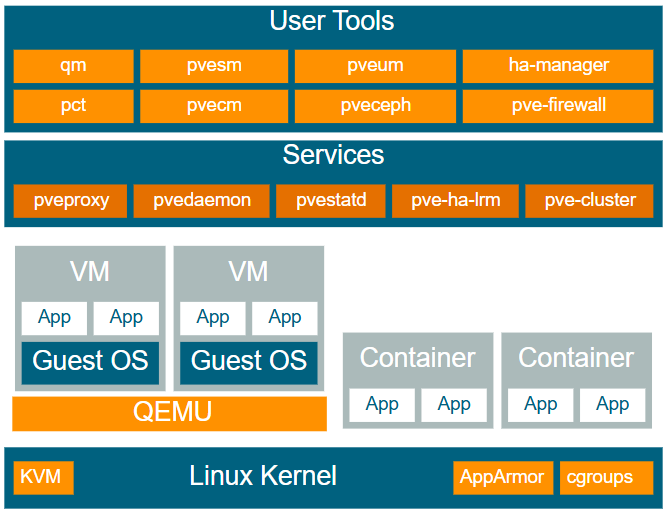
\includegraphics[width=0.8\linewidth]{pve-software-stack}
	\caption{Proxmox 软件栈}
	\label{fig:pve-software-stack}
\end{figure}

\section{集中管理}

虽然许多人从单个节点开始，但 Proxmox VE 可以扩展到大型集群节点。集群堆栈完全集成，并随默认安装一起提供。

\begin{description}[leftmargin=2cm]
	\item[独特的多主设计] 集成的基于 Web 的管理界面为您提供所有 KVM 客户机和 Linux 容器以及整个集群的清晰概览。您可以从 GUI 轻松管理 VM 和容器、存储或集群。无需安装单独的、复杂的、昂贵的管理服务器。
	\item[Proxmox 集群文件系统 (pmxcfs)] Proxmox VE 使用独特的 Proxmox 集群文件系统 (pmxcfs)，这是一个用于存储配置文件的数据库驱动文件系统。这使您能够存储数千个虚拟机的配置。通过使用 corosync，这些文件在所有集群节点上实时复制。文件系统将所有数据存储在磁盘上的持久数据库中，尽管如此，数据的副本驻留在 RAM 中，最大存储大小为 30MB——足以容纳数千个 VM。
	\item[基于 Web 的管理界面] Proxmox VE 简单易用。管理任务可以通过包含的基于 Web 的管理界面完成——无需安装单独的管理工具或任何带有大型数据库的额外管理节点。多主工具允许您从集群的任何节点管理整个集群。
	\item[命令行] 对于习惯使用 Unix shell 或 Windows Powershell 的高级用户，Proxmox VE 提供了一个命令行界面来管理虚拟环境的所有组件。此命令行界面具有智能的制表符补全功能和完整的 UNIX 手册页文档。
	\item[REST API] Proxmox VE 使用 RESTful API。我们选择 JSON 作为主要数据格式，整个 API 使用 JSON Schema 正式定义。这使得第三方管理工具能够快速轻松地集成。
	\item[基于角色的管理] 您可以使用基于角色的用户和权限管理为所有对象（如 VM、存储、节点等）定义细粒度的访问权限。
	\item[认证域] Proxmox VE 支持多种认证源，如 Microsoft Active Directory、LDAP、Linux PAM 标准认证或内置的 Proxmox VE 认证服务器。
\end{description}

\section{灵活的存储}

Proxmox VE 存储模型非常灵活。虚拟机映像可以存储在一个或多个本地存储上，也可以存储在 NFS 和 SAN 等共享存储上。没有限制，您可以根据需要配置任意数量的存储定义。您可以使用 Debian Linux 可用的所有存储技术。

将 VM 存储在共享存储上的一个主要好处是能够实时迁移正在运行的机器而无需任何停机时间，因为集群中的所有节点都可以直接访问 VM 磁盘映像。

我们目前支持以下网络存储类型：
\begin{itemize}[leftmargin=2cm]
	\item LVM 组（使用 iSCSI 目标的网络支持）
	\item iSCSI 目标
	\item NFS 共享
	\item CIFS 共享
	\item Ceph RBD
	\item CephFS
	\item 直接使用 iSCSI LUN 或光纤连接 SAN
\end{itemize}

支持的本地存储类型有：
\begin{itemize}[leftmargin=2cm]
	\item LVM 组（本地支持设备，如块设备、FC 设备、DRBD 等）
	\item 目录（现有文件系统上的存储）
	\item ZFS
\end{itemize}

\section{集成备份和恢复}

集成的备份工具 (\texttt{vzdump}) 为运行中的容器和 KVM 客户机创建一致的快照。它基本上创建了 VM 或 CT 数据的存档，其中包括 VM/CT 配置文件。

此外，Proxmox Backup Server 集成提供了高级功能，包括组合完整备份和数据去重、执行客户端加密、备份到磁带或 S3 对象存储，以及与其他异地 Proxmox Backup Server 安装同步。

QEMU/KVM 实时备份适用于所有存储类型，包括 NFS、CIFS、iSCSI LUN、Ceph RBD 上的 VM 映像。新的备份格式经过优化，可快速有效地存储 VM 备份（稀疏文件、无序数据、最小化 I/O）。

\section{高可用性集群}

多节点 Proxmox VE HA 集群支持定义高可用的虚拟服务器。Proxmox VE HA 集群基于经过验证的 Linux HA 技术，提供稳定可靠的 HA 服务。

\section{灵活的网络}

Proxmox VE 使用桥接网络模型。所有 VM 可以共享一个桥接，就像来自每个客户机的虚拟网络电缆都插入到同一个交换机中一样。为了将 VM 连接到外部世界，桥接器连接到物理网卡并分配 TCP/IP 配置。

为了进一步提高灵活性，可以使用 VLAN（IEEE 802.1q）和网络绑定/聚合。通过这种方式，可以为 Proxmox VE 主机构建复杂的、灵活的虚拟网络，充分利用 Linux 网络堆栈的全部功能。

\section{集成防火墙}

集成的防火墙允许您在任意 VM 或容器接口上过滤网络数据包。可以将常见的防火墙规则集分组为"安全组"。

\section{超融合基础设施}

Proxmox VE 是一个虚拟化平台，紧密集成计算、存储和网络资源，管理高可用集群、备份/恢复以及灾难恢复。所有组件都是软件定义的，并且相互兼容。

因此，可以通过集中式 Web 管理界面像管理单个系统一样管理它们。这些功能使 Proxmox VE 成为部署和管理开源超融合基础设施的理想选择。

\subsection{超融合基础设施的优势}

超融合基础设施 (HCI) 特别适用于高基础设施需求与低管理预算相结合的部署，例如远程和分支机构环境的分布式设置，或虚拟私有云和公有云。

HCI 提供以下优势：
\begin{itemize}[leftmargin=2cm]
	\item \textbf{可扩展性}：无缝扩展计算、网络和存储设备（即快速独立地扩展服务器和存储）。
	\item \textbf{低成本}：Proxmox VE 是开源的，并集成了计算、存储、网络、备份和管理中心等所有组件。它可以替代昂贵的计算/存储基础设施。
	\item \textbf{数据保护和效率}：集成了备份和灾难恢复等服务。
	\item \textbf{简单性}：易于配置和集中管理。
	\item \textbf{开源}：无供应商锁定。
\end{itemize}

\subsection{超融合基础设施存储}

Proxmox VE 紧密集成支持部署超融合存储基础设施。例如，您可以使用 Web 界面部署和管理以下两种存储技术：

\begin{itemize}[leftmargin=2cm]
	\item \textbf{Ceph}：一个自修复和自管理的共享、可靠且高度可扩展的存储系统。
	\item \textbf{ZFS}：一个组合的文件系统和逻辑卷管理器，具有广泛的数据损坏保护、各种 RAID 模式、快速且便宜的快照等功能。
\end{itemize}

\section{为什么选择开源}

Proxmox VE 使用 Linux 内核，基于 Debian GNU/Linux 发行版。Proxmox VE 的源代码根据 GNU Affero 通用公共许可证第 3 版发布。这意味着您可以随时检查源代码或自己为项目做出贡献。

在 Proxmox，我们致力于尽可能使用开源软件。使用开源软件保证了对所有功能的完全访问——以及高安全性和可靠性。我们认为每个人都应该有权访问软件的源代码以运行它、在其上构建或向项目提交更改。

开源软件还有助于降低成本，并使您的基础设施独立于单个供应商。

\section{Proxmox VE 的优势}

\begin{itemize}[leftmargin=2cm]
	\item 开源软件
	\item 无供应商锁定
	\item Linux 内核
	\item 安装快速且易于使用
	\item 基于 Web 的管理界面
	\item REST API
	\item 庞大的活跃社区
	\item 管理成本低，部署简单
\end{itemize}

\section{获取帮助}

\subsection{Proxmox VE Wiki}

主要信息来源是 Proxmox VE Wiki。它结合了参考文档和用户贡献的内容。

\subsection{社区支持论坛}

Proxmox VE 本身是完全开源的，因此我们始终鼓励用户使用 Proxmox VE 社区论坛讨论和分享他们的知识。该论坛由 Proxmox 支持团队管理，拥有来自世界各地的大量用户群。

\subsection{邮件列表}

这是通过电子邮件与 Proxmox VE 社区快速沟通的方式。

\begin{itemize}[leftmargin=2cm]
	\item 用户邮件列表：Proxmox VE 用户列表
	\item 开发者邮件列表：Proxmox VE 开发讨论
\end{itemize}

\subsection{商业支持}

Proxmox Server Solutions GmbH 还提供企业支持，作为 Proxmox VE 订阅服务计划提供。所有订阅用户都可以访问 Proxmox VE 企业仓库，并通过基本、标准或高级订阅访问 Proxmox 客户门户。

\subsection{Bug 跟踪器}

Proxmox 在 https://bugzilla.proxmox.com 运行公共 Bug 跟踪器。如果出现问题，请在那里提交报告。

\section{项目历史}

该项目始于 2007 年，第一个稳定版本于 2008 年发布。当时我们使用 OpenVZ 作为容器，使用 QEMU 和 KVM 作为虚拟机。集群功能有限，用户界面也很简单（服务器生成的网页）。

但我们很快使用 Corosync 集群堆栈开发了新功能，引入新的 Proxmox 集群文件系统 (pmxcfs) 是一个重大进步，因为它完全向用户隐藏了集群复杂性。管理 16 个节点的集群与管理单个节点一样简单。

我们新的 REST API 的引入，以及使用 JSON-Schema 编写的完整声明式规范，使其他人能够将 Proxmox VE 集成到他们的基础设施中，并轻松提供额外的服务。

此外，新的 REST API 使得可以用现代客户端单页应用程序（使用 JavaScript）替换原始用户界面成为可能。我们还用 noVNC 替换了旧的基于 Java 的 VNC 控制台代码。因此，您只需要一个 Web 浏览器即可管理您的 VM。

对各种存储类型的支持是另一项重大任务。值得注意的是，Proxmox VE 于 2014 年成为第一个默认提供 ZFS on Linux 的发行版。另一个里程碑是能够在管理程序节点上运行和管理 Ceph 存储。这种设置极具成本效益。

\section{改进 Proxmox VE 文档}

欢迎对 Proxmox VE 文档做出贡献和改进。有几种方法可以贡献：

\begin{itemize}[leftmargin=2cm]
	\item 如果您在本文档中发现错误或其他改进空间，请在 Proxmox Bug 跟踪器中提交错误以提出更正建议。
	\item 对于特定的设置、操作指南或教程，Wiki 是贡献的正确选择。
	\item 对于对所有用户都有帮助的一般内容，请为参考文档提出您的贡献。
\end{itemize}

\section{翻译 Proxmox VE}

Proxmox VE 用户界面默认使用英语。但是，由于社区的贡献，其他语言的翻译也可用。我们欢迎任何支持来添加新语言、翻译最新功能以及改进不完整或不一致的翻译。

我们使用 gettext 来管理翻译文件。Poedit 等工具提供了编辑翻译文件的良好用户界面，但您可以使用任何您熟悉的编辑器。翻译不需要编程知识。




\mainmatter


% ===== 第01章补充内容 =====


% 1.1. Central Management
\subsection{集中式管理 (Central Management)}

\textbf{English Original:}

While many people start with a single node, Proxmox VE can scale out to a
large set of clustered nodes. The cluster stack is fully integrated
and ships with the default installation.

Proxmox VE uses the unique Proxmox Cluster file system (pmxcfs), a
database-driven file system for storing configuration files. This
enables you to store the configuration of thousands of virtual
machines. By using corosync, these files are replicated in real time
on all cluster nodes. The file system stores all data inside a
persistent database on disk, nonetheless, a copy of the data resides
in RAM which provides a maximum storage size of 30MB - more than
enough for thousands of VMs.

Proxmox VE is the only virtualization platform using this unique
cluster file system.

\textbf{中文翻译:}

虽然许多人从单个节点开始，但 Proxmox VE 可以扩展到大量集群节点。集群堆栈完全集成，并随默认安装一起提供。

Proxmox VE 使用独特的 Proxmox 集群文件系统，这是一个用于存储配置文件的数据库驱动文件系统。这使您能够存储数千台虚拟机的配置。通过使用 corosync，这些文件会在所有集群节点上实时复制。文件系统将所有数据存储在磁盘上的持久数据库中，但数据的一个副本驻留在 RAM 中，提供最大 30MB 的存储空间 - 足以容纳数千台虚拟机。

Proxmox VE 是唯一使用这种独特集群文件系统的虚拟化平台。



% 1.2. Flexible Storage
\subsection{灵活存储 (Flexible Storage)}

\textbf{English Original:}

The Proxmox VE storage model is very flexible. Virtual machine images
can either be stored on one or several local storages or on shared
storage like NFS and on SAN. There are no limits, you may configure as
many storage definitions as you like. You can use all storage
technologies available for Debian Linux.

One major benefit of storing VMs on shared storage is the ability to
live-migrate running machines without any downtime, as all nodes in
the cluster have direct access to VM disk images.

We currently support the following Network storage types:

Local storage types supported are:

\begin{itemize}
\item LVM Group (network backing with iSCSI targets)
\item iSCSI target
\item NFS Share
\item CIFS Share
\item Ceph RBD
\item CephFS
\item Directly use iSCSI LUNs or Fibre Attached SANs.
\end{itemize}
\begin{itemize}
\item LVM Group (local backing devices like block devices, FC devices, DRBD, etc.)
\item Directory (storage on existing filesystem)
\item ZFS
\end{itemize}

\textbf{中文翻译:}

Proxmox VE 存储模型非常灵活。虚拟机映像可以存储在一个或多个本地存储上，也可以存储在共享存储上，如 NFS 和 SAN。没有限制，您可以根据需要配置任意数量的存储定义。您可以使用 Debian Linux 可用的所有存储技术。

将虚拟机存储在共享存储上的一个主要好处是能够实时迁移正在运行的机器而不会停机，因为集群中的所有节点都可以直接访问虚拟机磁盘映像。

我们目前支持以下网络存储类型：

支持的本地存储类型有：

\begin{itemize}
\item LVM 组（使用 iSCSI 目标的网络后端）
\item iSCSI 目标
\item NFS 共享
\item CIFS 共享
\item Ceph RBD
\item CephFS
\item 直接使用 iSCSI LUN 或光纤通道连接的 SAN。
\end{itemize}
\begin{itemize}
\item LVM 组（本地后端设备，如块设备、FC 设备、DRBD 等）
\item 目录（现有文件系统上的存储）
\item ZFS
\end{itemize}


% 1.3. Integrated Backup and Restore
\subsection{集成备份和恢复 (Integrated Backup and Restore)}

\textbf{English Original:}

The integrated backup tool (vzdump) creates consistent snapshots of running
Containers and KVM guests. It basically creates an archive of the VM or CT data
which includes the VM/CT configuration files.

Additionally, the Proxmox Backup Server integration provides
advanced features, including the ability to combine full backups and data
deduplication, perform client-side encryption, back up to tape or S3 object
storage, and sync with other offsite Proxmox Backup Server installations.

QEMU/KVM live backup works for all storage types including VM images on
NFS, CIFS, iSCSI LUN, Ceph RBD. The new backup format is optimized for storing
VM backups fast and effective (sparse files, out of order data, minimized I/O).

\texttt{vzdump}

\textbf{中文翻译:}

集成备份工具创建正在运行的容器和 KVM 客户机的一致性快照。它基本上创建虚拟机或容器数据的归档，其中包括虚拟机/容器的配置文件。

此外，Proxmox Backup Server 集成提供了高级功能，包括组合完整备份和数据去重的能力、执行客户端加密、备份到磁带或 S3 对象存储，以及与其他异地 Proxmox Backup Server 安装同步。

QEMU/KVM 实时备份适用于所有存储类型，包括 NFS、CIFS、iSCSI LUN、Ceph RBD 上的虚拟机映像。新的备份格式针对快速有效地存储虚拟机备份进行了优化（稀疏文件、乱序数据、最小化 I/O）。

\texttt{vzdump}


% 1.4. High Availability Cluster
\subsection{高可用性集群 (High Availability Cluster)}

\textbf{English Original:}

A multi-node Proxmox VE HA Cluster enables the definition of highly
available virtual servers. The Proxmox VE HA Cluster is based on
proven Linux HA technologies, providing stable and reliable HA
services.

\textbf{中文翻译:}

多节点 Proxmox VE HA 集群使您能够定义高可用虚拟服务器。Proxmox VE HA 集群基于经过验证的 Linux HA 技术，提供稳定可靠的 HA 服务。



% 1.5. Flexible Networking
\subsection{灵活网络 (Flexible Networking)}

\textbf{English Original:}

Proxmox VE uses a bridged networking model. All VMs can share one
bridge as if virtual network cables from each guest were all plugged
into the same switch. For connecting VMs to the outside world, bridges
are attached to physical network cards and assigned a TCP/IP
configuration.

For further flexibility, VLANs (IEEE 802.1q) and network
bonding/aggregation are possible. In this way it is possible to build
complex, flexible virtual networks for the Proxmox VE hosts,
leveraging the full power of the Linux network stack.

\textbf{中文翻译:}

Proxmox VE 使用桥接网络模型。所有虚拟机可以共享一个网桥，就像每台客户机的虚拟网络电缆都插入到同一个交换机中一样。为了将虚拟机连接到外部世界，网桥会附加到物理网卡并分配 TCP/IP 配置。

为了进一步增加灵活性，可以使用 VLAN（IEEE 802.1q）和网络绑定/聚合。通过这种方式，可以为 Proxmox VE 主机构建复杂、灵活的虚拟网络，充分利用 Linux 网络堆栈的强大功能。



% 1.6. Integrated Firewall
\subsection{. Integrated Firewall}
The integrated firewall allows you to filter network packets on
any VM or Container interface. Common sets of firewall rules can
be grouped into “security groups”.



% 1.7. Hyper-converged Infrastructure
\subsection{超融合基础设施 (Hyper-converged Infrastructure)}

\textbf{English Original:}

Proxmox VE is a virtualization platform that tightly integrates compute, storage and
networking resources, manages highly available clusters, backup/restore as well
as disaster recovery. All components are software-defined and compatible with
one another.

Therefore it is possible to administrate them like a single system via the
centralized web management interface. These capabilities make Proxmox VE an ideal
choice to deploy and manage an open source
hyper-converged infrastructure.

A hyper-converged infrastructure (HCI) is especially useful for deployments in
which a high infrastructure demand meets a low administration budget, for
distributed setups such as remote and branch office environments or for virtual
private and public clouds.

HCI provides the following advantages:

Proxmox VE has tightly integrated support for deploying a hyper-converged storage
infrastructure. You can, for example, deploy and manage the following two
storage technologies by using the web interface only:

Besides above, Proxmox VE has support to integrate a wide range of
additional storage technologies. You can find out about them in the
Storage Manager chapter.

\begin{itemize}
\item Scalability: seamless expansion of compute, network and storage devices (i.e.
  scale up servers and storage quickly and independently from each other).
\item Low cost: Proxmox VE is open source and integrates all components you need such as
  compute, storage, networking, backup, and management center. It can replace
  an expensive compute/storage infrastructure.
\item Data protection and efficiency: services such as backup and disaster recovery
  are integrated.
\item Simplicity: easy configuration and centralized administration.
\item Open Source: No vendor lock-in.
\end{itemize}
\begin{itemize}
\item Ceph: a both self-healing and self-managing shared, reliable and highly
  scalable storage system. Checkout
  how to manage Ceph services on Proxmox VE nodes
\item ZFS: a combined file system and logical volume manager with extensive
  protection against data corruption, various RAID modes, fast and cheap
  snapshots - among other features. Find out
  how to leverage the power of ZFS on Proxmox VE nodes.
\end{itemize}

\textbf{中文翻译:}

Proxmox VE 是一个虚拟化平台，紧密集成计算、存储和网络资源，管理高可用集群、备份/恢复以及灾难恢复。所有组件都是软件定义的，并且彼此兼容。

因此，可以通过集中式 Web 管理界面像管理单个系统一样管理它们。这些功能使 Proxmox VE 成为部署和管理开源超融合基础设施的理想选择。

超融合基础设施（HCI）对于基础设施需求高但管理预算低的部署特别有用，例如远程和分支机构环境的分布式设置，或虚拟私有云和公共云。

HCI 提供以下优势：

Proxmox VE 具有紧密集成的支持，用于部署超融合存储基础设施。例如，您可以仅使用 Web 界面部署和管理以下两种存储技术：

此外，Proxmox VE 支持集成广泛的额外存储技术。您可以在存储管理器章节中了解它们。

\begin{itemize}
\item 可扩展性：计算、网络和存储设备的无缝扩展（即快速且独立地扩展服务器和存储）。
\item 低成本：Proxmox VE 是开源的，集成了您需要的所有组件，如计算、存储、网络、备份和管理中心。它可以替代昂贵的计算/存储基础设施。
\item 数据保护和效率：备份和灾难恢复等服务已集成。
\item 简单性：易于配置和集中管理。
\item 开源：无供应商锁定。
\end{itemize}
\begin{itemize}
\item Ceph：一个自我修复和自我管理的共享、可靠和高度可扩展的存储系统。查看如何在 Proxmox VE 节点上管理 Ceph 服务。
\item ZFS：一个结合文件系统和逻辑卷管理器的系统，具有广泛的数据损坏保护、各种 RAID 模式、快速和廉价的快照等功能。了解如何在 Proxmox VE 节点上利用 ZFS 的强大功能。
\end{itemize}


% 1.8. Why Open Source
\subsection{为什么选择开源 (Why Open Source)}

\textbf{English Original:}

Proxmox VE uses a Linux kernel and is based on the Debian GNU/Linux
Distribution. The source code of Proxmox VE is released under the
GNU Affero General Public
License, version 3. This means that you are free to inspect the
source code at any time or contribute to the project yourself.

At Proxmox we are committed to use open source software whenever
possible. Using open source software guarantees full access to all
functionalities - as well as high security and reliability. We think
that everybody should have the right to access the source code of a
software to run it, build on it, or submit changes back to the
project. Everybody is encouraged to contribute while Proxmox ensures
the product always meets professional quality criteria.

Open source software also helps to keep your costs low and makes your
core infrastructure independent from a single vendor.

\textbf{中文翻译:}

Proxmox VE 使用 Linux 内核，并基于 Debian GNU/Linux 发行版。Proxmox VE 的源代码在 GNU Affero 通用公共许可证第 3 版下发布。这意味着您可以随时检查源代码或自己为项目做出贡献。

在 Proxmox，我们致力于尽可能使用开源软件。使用开源软件保证了对所有功能的完全访问 - 以及高安全性和可靠性。我们认为每个人都应该有权访问软件的源代码来运行它、基于它构建，或将更改提交回项目。每个人都受到鼓励做出贡献，而 Proxmox 确保产品始终符合专业质量标准。

开源软件还有助于保持低成本，并使您的核心基础设施独立于单一供应商。



% 1.9. Your benefits with Proxmox VE
\subsection{Proxmox VE 的优势 (Your benefits with Proxmox VE)}

\textbf{English Original:}

\begin{itemize}
\item Open source software
\item No vendor lock-in
\item Linux kernel
\item Fast installation and easy-to-use
\item Web-based management interface
\item REST API
\item Huge active community
\item Low administration costs and simple deployment
\end{itemize}

\textbf{中文翻译:}

\begin{itemize}
\item 开源软件
\item 无供应商锁定
\item Linux 内核
\item 快速安装且易于使用
\item 基于 Web 的管理界面
\item REST API
\item 庞大的活跃社区
\item 低管理成本和简单部署
\end{itemize}


% 1.10. Getting Help
\subsection{获取帮助 (Getting Help)}

\textbf{English Original:}

The primary source of information is the Proxmox VE Wiki. It combines the reference
documentation with user contributed content.

Proxmox VE itself is fully open source, so we always encourage our users to discuss
and share their knowledge using the Proxmox VE Community Forum. The forum is moderated by the
Proxmox support team, and has a large user base from all around the world.
Needless to say, such a large forum is a great place to get information.

This is a fast way to communicate with the Proxmox VE community via email.

Proxmox VE is fully open source and contributions are welcome! The primary
communication channel for developers is the:

Proxmox Server Solutions GmbH also offers enterprise support available as
Proxmox VE Subscription Service Plans.
All users with a subscription get access to the Proxmox VE
Enterprise Repository, and—with a Basic, Standard
or Premium subscription—also to the Proxmox Customer Portal. The customer
portal provides help and support with guaranteed response times from the Proxmox VE
developers.

For volume discounts, or more information in general, please contact
sales@proxmox.com.

Proxmox runs a public bug tracker at https://bugzilla.proxmox.com. If an issue
appears, file your report there. An issue can be a bug as well as a request for
a new feature or enhancement. The bug tracker helps to keep track of the issue
and will send a notification once it has been solved.

\begin{itemize}
\item Mailing list for users:
  Proxmox VE User List
\end{itemize}

\textbf{中文翻译:}

主要的信息来源是 Proxmox VE Wiki。它将参考文档与用户贡献的内容结合起来。

Proxmox VE 本身是完全开源的，因此我们始终鼓励用户使用 Proxmox VE 社区论坛讨论和分享他们的知识。该论坛由 Proxmox 支持团队管理，拥有来自世界各地的庞大用户群。不用说，这样一个大型论坛是获取信息的好地方。

这是通过电子邮件与 Proxmox VE 社区快速交流的方式。

Proxmox VE 完全开源，欢迎贡献！开发人员的主要交流渠道是：

Proxmox Server Solutions GmbH 还提供企业支持，可作为 Proxmox VE 订阅服务计划使用。

所有订阅用户都可以访问 Proxmox VE 企业存储库，并且通过 Basic、Standard 或 Premium 订阅，还可以访问 Proxmox 客户门户。客户门户提供帮助和支持，并有 Proxmox VE 开发人员的保证响应时间。

对于批量折扣或一般更多信息，请联系 sales@proxmox.com。

Proxmox 在 https://bugzilla.proxmox.com 运行一个公共错误跟踪器。如果出现问题，请在那里提交您的报告。问题可以是错误，也可以是对新功能或增强的请求。错误跟踪器有助于跟踪问题，并在问题解决后发送通知。

\begin{itemize}
\item 用户邮件列表：
  Proxmox VE 用户列表
\end{itemize}
\begin{itemize}
\item Mailing list for developers:
  Proxmox VE development
  discussion
\end{itemize}

\textbf{中文翻译:}

\begin{itemize}
\item 开发人员邮件列表：
  Proxmox VE 开发讨论
\end{itemize}


% 1.11. Project History
\subsection{项目历史 (Project History)}

\textbf{English Original:}

The project started in 2007, followed by a first stable version in 2008. At the
time we used OpenVZ for containers, and QEMU with KVM for virtual machines. The
clustering features were limited, and the user interface was simple (server
generated web page).

But we quickly developed new features using the
Corosync cluster stack, and the
introduction of the new Proxmox cluster file system (pmxcfs) was a big step
forward, because it completely hides the cluster complexity from the user.
Managing a cluster of 16 nodes is as simple as managing a single node.

The introduction of our new REST API, with a complete declarative specification
written in JSON-Schema, enabled other people to integrate Proxmox VE into their
infrastructure, and made it easy to provide additional services.

Also, the new REST API made it possible to replace the original user interface
with a modern client side single-page application using JavaScript. We also
replaced the old Java based VNC console code with
noVNC. So you only need a web browser to manage
your VMs.

\textbf{中文翻译:}

该项目始于 2007 年，随后于 2008 年推出了第一个稳定版本。当时我们使用 OpenVZ 作为容器，使用 QEMU 和 KVM 作为虚拟机。集群功能有限，用户界面简单（服务器生成的网页）。

但我们很快使用 Corosync 集群堆栈开发了新功能，新的 Proxmox 集群文件系统的引入是一个巨大的进步，因为它完全向用户隐藏了集群复杂性。管理 16 个节点的集群与管理单个节点一样简单。

我们新的 REST API 的引入，以及用 JSON-Schema 编写的完整声明性规范，使其他人能够将 Proxmox VE 集成到他们的基础设施中，并轻松提供额外服务。

此外，新的 REST API 使我们能够使用 JavaScript 用现代客户端单页应用程序替换原始用户界面。我们还用 noVNC 替换了旧的基于 Java 的 VNC 控制台代码。因此，您只需要一个 Web 浏览器即可管理您的虚拟机。

The support for various storage types is another big task. Notably, Proxmox VE was
the first distribution to ship ZFS on Linux by default
in 2014. Another milestone was the ability to run and manage
Ceph storage on the hypervisor nodes. Such setups are
extremely cost effective.

When our project started we were among the first companies providing commercial
support for KVM. The KVM project itself continuously evolved, and is now a
widely used hypervisor. New features arrive with each release. We developed the
KVM live backup feature, which makes it possible to create snapshot backups on
any storage type.

The most notable change with version 4.0 was the move from OpenVZ to
LXC. Containers are now deeply integrated, and
they can use the same storage and network features as virtual machines. At the
same time we introduced the easy-to-use
High Availability (HA) manager, simplifying the
configuration and management of highly available setups.

During the development of Proxmox VE 5 the asynchronous
storage replication as well as automated
certificate management using ACME/Let’s
Encrypt were introduced, among many other features.

The Software Defined Network (SDN) stack was developed in
cooperation with our community. It was integrated into the web interface as
an experimental feature in version 6.2, simplifying the management of
sophisticated network configurations. Since version 8.1, the SDN integration is
fully supported and installed by default.

2020 marked the release of a new project, the
Proxmox
Backup Server, written in the Rust programming language. Proxmox Backup Server
is deeply integrated with Proxmox VE and significantly improves backup capabilities
by implementing incremental backups, deduplication, and much more.

\textbf{中文翻译:}

对各种存储类型的支持是另一项重大任务。值得注意的是，Proxmox VE 是第一个在 2014 年默认在 Linux 上提供 ZFS 的发行版。另一个里程碑是能够在虚拟机管理程序节点上运行和管理 Ceph 存储。这种设置非常具有成本效益。

当我们的项目开始时，我们是首批为 KVM 提供商业支持的公司之一。KVM 项目本身不断发展，现在是一个广泛使用的虚拟机管理程序。每个版本都会带来新功能。我们开发了 KVM 实时备份功能，这使得可以在任何存储类型上创建快照备份。

版本 4.0 最显著的变化是从 OpenVZ 转移到 LXC。容器现在已深度集成，并且可以使用与虚拟机相同的存储和网络功能。同时，我们引入了易于使用的高可用性（HA）管理器，简化了高可用性设置的配置和管理。

在 Proxmox VE 5 的开发过程中，引入了异步存储复制以及使用 ACME/Let's Encrypt 的自动化证书管理，以及许多其他功能。

软件定义网络（SDN）堆栈是与我们的社区合作开发的。它在版本 6.2 中作为实验性功能集成到 Web 界面中，简化了复杂网络配置的管理。自版本 8.1 起，SDN 集成得到完全支持并默认安装。

2020 年标志着新项目的发布，即 Proxmox Backup Server，使用 Rust 编程语言编写。Proxmox Backup Server 与 Proxmox VE 深度集成，通过实现增量备份、重复数据删除等功能，显著提高了备份能力。

Another new tool, the Proxmox
Offline Mirror, was released in 2022, enabling subscriptions for systems which
have no connection to the public internet.

\textbf{中文翻译:}

另一个新工具，Proxmox Offline Mirror，于 2022 年发布，为无法连接到公共互联网的系统提供订阅服务。

The highly requested dark theme for the web interface was introduced in 2023.
Later that year, version 8.0 integrated access to the Ceph enterprise
repository. Now access to the most stable Ceph repository comes with any
Proxmox VE subscription.

\textbf{中文翻译:}

2023 年引入了备受期待的 Web 界面深色主题。同年晚些时候，版本 8.0 集成了对 Ceph 企业存储库的访问。现在，任何 Proxmox VE 订阅都可以访问最稳定的 Ceph 存储库。

Automated and unattended installation for the official
ISO installer was introduced in version 8.2,
significantly simplifying large deployments of Proxmox VE.

\textbf{中文翻译:}

版本 8.2 引入了官方 ISO 安装程序的自动和无人值守安装，大大简化了 Proxmox VE 的大规模部署。

With the import wizard, equally introduced in
version 8.2, users can easily and efficiently migrate guests directly from other
hypervisors like VMware ESXi [1].

\textbf{中文翻译:}

通过同样在版本 8.2 中引入的导入向导，用户可以轻松高效地直接从 VMware ESXi 等其他虚拟机管理程序迁移客户机 [1]。
Additionally, archives in Open Virtualization Format (OVF/OVA) can now be
directly imported from file-based storages in the web interface.

\textbf{中文翻译:}

此外，现在可以直接从 Web 界面中的基于文件的存储导入 Open Virtualization Format (OVF/OVA) 格式的归档文件。

[1] Migrate to Proxmox VE

\textbf{中文翻译:}

[1] 迁移到 Proxmox VE
https://pve.proxmox.com/wiki/Migrate\_to\_Proxmox\_VE



% 1.12. Improving the Proxmox VE Documentation
\subsection{. Improving the Proxmox VE Documentation}
Contributions and improvements to the Proxmox VE documentation are always welcome.
There are several ways to contribute.

If you find errors or other room for improvement in this documentation, please
file a bug at the Proxmox bug tracker to propose
a correction.

If you want to propose new content, choose one of the following options:

If you are interested in working on the Proxmox VE codebase, the
Developer Documentation wiki article will
show you where to start.

\begin{itemize}
\item The wiki: For specific setups, how-to guides, or tutorials the wiki   is the
right option to contribute.
\item The reference documentation: For general content that will be   helpful to all
  users please propose your contribution for the   reference documentation. This
  includes all information about how to install, configure, use, and
  troubleshoot Proxmox VE features. The reference documentation is written in the
  asciidoc format. To edit the
  documentation you need to clone the git repository at
  git://git.proxmox.com/git/pve-docs.git; then follow the
  README.adoc
  document.
\end{itemize}
\texttt{git://git.proxmox.com/git/pve-docs.git}


% 1.13. Translating Proxmox VE
\subsection{. Translating Proxmox VE}
\subsubsection{. Translating with git}
\subsubsection{. Translating without git}
\subsubsection{. Testing the Translation}
\subsubsection{. Sending the Translation}
The Proxmox VE user interface is in English by default. However, thanks to the
contributions of the community, translations to other languages are also available.
We welcome any support in adding new languages, translating the latest features, and
improving incomplete or inconsistent translations.

We use gettext for the management of the
translation files. Tools like Poedit offer a nice user
interface to edit the translation files, but you can use whatever editor you’re
comfortable with. No programming knowledge is required for translating.

The language files are available as a
git repository. If you are familiar
with git, please contribute according to our
Developer Documentation.

You can create a new translation by doing the following (replace <LANG> with the
language ID):

Or you can edit an existing translation, using the editor of your choice:

Even if you are not familiar with git, you can help translate Proxmox VE.
To start, you can download the language files
here. Find the
language you want to improve, then right click on the "raw" link of this language
file and select Save Link As…. Make your changes to the file, and then
send your final translation directly to office(at)proxmox.com, together with a
signed
contributor license agreement.

In order for the translation to be used in Proxmox VE, you must first translate
the .po file into a .js file. You can do this by invoking the following script,
which is located in the same repository:

The resulting file pve-lang-xx.js can then be copied to the directory
/usr/share/pve-i18n, on your proxmox server, in order to test it out.

Alternatively, you can build a deb package by running the following command from
the root of the repository:

For either of these methods to work, you need to have the following
perl packages installed on your system. For Debian/Ubuntu:

You can send the finished translation (.po file) to the Proxmox team at the address
office(at)proxmox.com, along with a signed contributor license agreement.
Alternatively, if you have some developer experience, you can send it as a
patch to the Proxmox VE development mailing list. See
Developer Documentation.

\texttt{.po}
\texttt{.js}
\texttt{pve-lang-xx.js}
\texttt{/usr/share/pve-i18n}
\texttt{.po}
\begin{verbatim}
# git clone git://git.proxmox.com/git/proxmox-i18n.git
# cd proxmox-i18n
# make init-<LANG>.po
\end{verbatim}
\begin{verbatim}
# poedit <LANG>.po
\end{verbatim}
\begin{verbatim}
# ./po2js.pl -t pve xx.po >pve-lang-xx.js
\end{verbatim}
\begin{verbatim}
# make deb
\end{verbatim}
\begin{verbatim}
# apt-get install perl liblocale-po-perl libjson-perl
\end{verbatim}




% ===== 第02章补充内容 =====


% 2.1. System Requirements
\subsection{系统要求 (System Requirements)}
\subsubsection{. Minimum Requirements, for Evaluation}
\subsubsection{. Recommended System Requirements}
\subsubsection{. Simple Performance Overview}
\subsubsection{. Supported Web Browsers for Accessing the Web Interface}
\textbf{English Original:}

We recommend using high quality server hardware, when running Proxmox VE in
production. To further decrease the impact of a failed host, you can run Proxmox VE in
a cluster with highly available (HA) virtual machines and containers.

Proxmox VE can use local storage (DAS), SAN, NAS, and distributed storage like Ceph
RBD. For details see chapter storage.

These minimum requirements are for evaluation purposes only and should not be
used in production.

VM storage:

To get an overview of the CPU and hard disk performance on an installed Proxmox VE
system, run the included pveperf tool.

This is just a very quick and general benchmark. More detailed tests are
recommended, especially regarding the I/O performance of your system.

To access the web-based user interface, we recommend using one of the following
browsers:

When accessed from a mobile device, Proxmox VE will show a lightweight, touch-based
interface.

\begin{itemize}
\item CPU: 64bit (Intel 64 or AMD64)
\item Intel VT/AMD-V capable CPU/motherboard for KVM full virtualization support
\item RAM: 1 GB RAM, plus additional RAM needed for guests
\item Hard drive
\item One network card (NIC)
\end{itemize}
\begin{itemize}
\item Intel 64 or AMD64 with Intel VT/AMD-V CPU flag.
\item Memory: Minimum 2 GB for the OS and Proxmox VE services, plus designated memory for
  guests. For Ceph and ZFS, additional memory is required; approximately 1GB of
  memory for every TB of used storage.
\item Fast and redundant storage, best results are achieved with SSDs.
\item OS storage: Use a hardware RAID with battery protected write cache (“BBU”)
  or non-RAID with ZFS (optional SSD for ZIL).
\item VM storage:

For local storage, use either a hardware RAID with battery backed write cache
  (BBU) or non-RAID for ZFS and Ceph. Neither ZFS nor Ceph are compatible with a
  hardware RAID controller.

Shared and distributed storage is possible.

SSDs with Power-Loss-Protection (PLP) are recommended for good performance.
  Using consumer SSDs is discouraged.
\item For local storage, use either a hardware RAID with battery backed write cache
  (BBU) or non-RAID for ZFS and Ceph. Neither ZFS nor Ceph are compatible with a
  hardware RAID controller.
\item Shared and distributed storage is possible.
\item SSDs with Power-Loss-Protection (PLP) are recommended for good performance.
  Using consumer SSDs is discouraged.
\item Redundant (Multi-)Gbit NICs, with additional NICs depending on the preferred
  storage technology and cluster setup.
\item For PCI(e) passthrough the CPU needs to support the VT-d/AMD-d flag.
\end{itemize}
\begin{itemize}
\item For local storage, use either a hardware RAID with battery backed write cache
  (BBU) or non-RAID for ZFS and Ceph. Neither ZFS nor Ceph are compatible with a
  hardware RAID controller.
\item Shared and distributed storage is possible.
\item SSDs with Power-Loss-Protection (PLP) are recommended for good performance.
  Using consumer SSDs is discouraged.
\end{itemize}
\begin{itemize}
\item Firefox, a release from the current year, or the latest Extended Support Release
\item Chrome, a release from the current year
\item Microsoft’s currently supported version of Edge
\item Safari, a release from the current year
\end{itemize}
\texttt{pveperf}

\textbf{中文翻译:}

在生产环境中运行 Proxmox VE 时，我们建议使用高质量的服务器硬件。为了进一步减少主机故障的影响，您可以在具有高可用性（HA）虚拟机和容器的集群中运行 Proxmox VE。

Proxmox VE 可以使用本地存储（DAS）、SAN、NAS 和分布式存储（如 Ceph RBD）。有关详细信息，请参阅存储章节。

这些最低要求仅用于评估目的，不应在生产环境中使用。

虚拟机存储：

要了解已安装的 Proxmox VE 系统上的 CPU 和硬盘性能，请运行随附的 pveperf 工具。

这只是一个非常快速的通用基准测试。建议进行更详细的测试，尤其是关于系统的 I/O 性能。

要访问基于 Web 的用户界面，我们建议使用以下浏览器之一：

从移动设备访问时，Proxmox VE 将显示轻量级、基于触摸的界面。

\begin{itemize}
\item CPU：64 位（Intel 64 或 AMD64）
\item 支持 Intel VT/AMD-V 的 CPU/主板，用于 KVM 全虚拟化支持
\item 内存：1 GB RAM，加上客户机所需的额外 RAM
\item 硬盘
\item 一个网卡（NIC）
\end{itemize}
\begin{itemize}
\item Intel 64 或 AMD64，具有 Intel VT/AMD-V CPU 标志。
\item 内存：操作系统和 Proxmox VE 服务至少需要 2 GB，加上为客户机分配的内存。对于 Ceph 和 ZFS，需要额外的内存；大约每 TB 已用存储空间需要 1GB 内存。
\item 快速且冗余的存储，使用 SSD 可获得最佳效果。
\item 操作系统存储：使用带有电池保护写入缓存（"BBU"）的硬件 RAID 或带有 ZFS 的非 RAID（ZIL 可选使用 SSD）。
\item 虚拟机存储：

对于本地存储，使用带有电池备份写入缓存（BBU）的硬件 RAID 或用于 ZFS 和 Ceph 的非 RAID。ZFS 和 Ceph 都与硬件 RAID 控制器不兼容。

可以使用共享和分布式存储。

建议使用具有掉电保护（PLP）的 SSD 以获得良好的性能。不建议使用消费级 SSD。
\item 对于本地存储，使用带有电池备份写入缓存（BBU）的硬件 RAID 或用于 ZFS 和 Ceph 的非 RAID。ZFS 和 Ceph 都与硬件 RAID 控制器不兼容。
\item 可以使用共享和分布式存储。
\item 建议使用具有掉电保护（PLP）的 SSD 以获得良好的性能。不建议使用消费级 SSD。
\item 冗余（多）千兆网卡，根据首选存储技术和集群设置需要额外的网卡。
\item 对于 PCI(e) 直通，CPU 需要支持 VT-d/AMD-d 标志。
\end{itemize}
\begin{itemize}
\item 对于本地存储，使用带有电池备份写入缓存（BBU）的硬件 RAID 或用于 ZFS 和 Ceph 的非 RAID。ZFS 和 Ceph 都与硬件 RAID 控制器不兼容。
\item 可以使用共享和分布式存储。
\item 建议使用具有掉电保护（PLP）的 SSD 以获得良好的性能。不建议使用消费级 SSD。
\end{itemize}
\begin{itemize}
\item Firefox，本年度发布的版本，或最新的扩展支持版本
\item Chrome，本年度发布的版本
\item Microsoft 当前支持的 Edge 版本
\item Safari，本年度发布的版本
\end{itemize}
\texttt{pveperf}


% 2.2. Prepare Installation Media
\subsection{准备安装媒体 (Prepare Installation Media)}

\textbf{English Original:}
\subsubsection{. Prepare a USB Flash Drive as Installation Medium}
\subsubsection{. Instructions for GNU/Linux}
\subsubsection{. Instructions for macOS}
\subsubsection{. Instructions for Windows}
Download the installer ISO image from: https://www.proxmox.com/en/downloads/proxmox-virtual-environment/iso

The Proxmox VE installation media is a hybrid ISO image. It works in two ways:

Using a USB flash drive to install Proxmox VE is the recommended way because it is
the faster option.

The flash drive needs to have at least 1 GB of storage available.

Do not use UNetbootin. It does not work with the Proxmox VE installation image.

Make sure that the USB flash drive is not mounted and does not
contain any important data.

On Unix-like operating system use the dd command to copy the ISO image to the
USB flash drive. First find the correct device name of the USB flash drive (see
below). Then run the dd command.

Be sure to replace /dev/XYZ with the correct device name and adapt the
input filename (if) path.

Be very careful, and do not overwrite the wrong disk!

There are two ways to find out the name of the USB flash drive. The first one is
to compare the last lines of the dmesg command output before and after
plugging in the flash drive. The second way is to compare the output of the
lsblk command. Open a terminal and run:

Then plug in your USB flash drive and run the command again:

A new device will appear. This is the one you want to use. To be on the extra
safe side check if the reported size matches your USB flash drive.

Open the terminal (query Terminal in Spotlight).

Convert the .iso file to .dmg format using the convert option of hdiutil,
for example:

macOS tends to automatically add .dmg to the output file name.

To get the current list of devices run the command:

Now insert the USB flash drive and run this command again to determine which
device node has been assigned to it. (e.g., /dev/diskX).

replace X with the disk number from the last command.

rdiskX, instead of diskX, in the last command is intended. It will
increase the write speed.

Etcher works out of the box. Download Etcher from https://etcher.io. It will
guide you through the process of selecting the ISO and your USB flash drive.

Rufus is a more lightweight alternative, but you need to use the DD mode to
make it work. Download Rufus from https://rufus.ie/. Either install it or use
the portable version. Select the destination drive and the Proxmox VE ISO file.

Once you Start you have to click No on the dialog asking to
download a different version of GRUB. In the next dialog select the DD mode.

\begin{itemize}
\item An ISO image file ready to burn to a CD or DVD.
\item A raw sector (IMG) image file ready to copy to a USB flash drive (USB stick).
\end{itemize}
\texttt{dd}
\texttt{dd}
\texttt{dmesg}
\texttt{lsblk}
\texttt{.iso}
\texttt{.dmg}
\texttt{hdiutil}
\begin{verbatim}
# dd bs=1M conv=fdatasync if=./proxmox-ve_*.iso of=/dev/XYZ
\end{verbatim}
\begin{verbatim}
# lsblk
\end{verbatim}
\begin{verbatim}
# lsblk
\end{verbatim}
\begin{verbatim}
# hdiutil convert proxmox-ve_*.iso -format UDRW -o proxmox-ve_*.dmg
\end{verbatim}
\begin{verbatim}
# diskutil list
\end{verbatim}
\begin{verbatim}
# diskutil list
# diskutil unmountDisk /dev/diskX
\end{verbatim}
\begin{verbatim}
# sudo dd if=proxmox-ve_*.dmg bs=1M of=/dev/rdiskX
\end{verbatim}

\textbf{中文翻译:}

从以下地址下载安装程序 ISO 镜像：https://www.proxmox.com/en/downloads/proxmox-virtual-environment/iso

Proxmox VE 安装媒体是一个混合 ISO 镜像。它有两种工作方式：

\begin{itemize}
\item 一个可刻录到 CD 或 DVD 的 ISO 镜像文件。
\item 一个可复制到 USB 闪存驱动器（U盘）的原始扇区（IMG）镜像文件。
\end{itemize}

使用 USB 闪存驱动器安装 Proxmox VE 是推荐的方式，因为它速度更快。

闪存驱动器需要至少 1 GB 的可用存储空间。

不要使用 UNetbootin。它与 Proxmox VE 安装镜像不兼容。

确保 USB 闪存驱动器未挂载且不包含任何重要数据。

在类 Unix 操作系统上，使用 dd 命令将 ISO 镜像复制到 USB 闪存驱动器。首先找到 USB 闪存驱动器的正确设备名称（见下文）。然后运行 dd 命令。

确保将 /dev/XYZ 替换为正确的设备名称，并调整输入文件名（if）路径。

要非常小心，不要覆盖错误的磁盘！

有两种方法可以找出 USB 闪存驱动器的名称。第一种是比较插入闪存驱动器前后 dmesg 命令输出的最后几行。第二种方法是比较 lsblk 命令的输出。打开终端并运行：

\begin{verbatim}
# lsblk
\end{verbatim}

然后插入您的 USB 闪存驱动器并再次运行该命令：

\begin{verbatim}
# lsblk
\end{verbatim}

会出现一个新设备。这就是您要使用的设备。为了更加安全，请检查报告的大小是否与您的 USB 闪存驱动器匹配。

\begin{verbatim}
# dd bs=1M conv=fdatasync if=./proxmox-ve_*.iso of=/dev/XYZ
\end{verbatim}

打开终端（在 Spotlight 中查询 Terminal）。

使用 hdiutil 的 convert 选项将 .iso 文件转换为 .dmg 格式，例如：

\begin{verbatim}
# hdiutil convert proxmox-ve_*.iso -format UDRW -o proxmox-ve_*.dmg
\end{verbatim}

macOS 倾向于自动为输出文件名添加 .dmg。

要获取当前设备列表，请运行命令：

\begin{verbatim}
# diskutil list
\end{verbatim}

现在插入 USB 闪存驱动器并再次运行此命令，以确定为其分配了哪个设备节点（例如 /dev/diskX）。

\begin{verbatim}
# diskutil list
# diskutil unmountDisk /dev/diskX
\end{verbatim}

将 X 替换为上一个命令中的磁盘编号。

\begin{verbatim}
# sudo dd if=proxmox-ve_*.dmg bs=1M of=/dev/rdiskX
\end{verbatim}

最后一条命令中的 rdiskX 而不是 diskX 是有意的。它将提高写入速度。

Etcher 可以直接使用。从 https://etcher.io 下载 Etcher。它将引导您完成选择 ISO 和 USB 闪存驱动器的过程。

Rufus 是一个更轻量级的替代方案，但您需要使用 DD 模式才能使其工作。从 https://rufus.ie/ 下载 Rufus。安装它或使用便携版本。选择目标驱动器和 Proxmox VE ISO 文件。

一旦开始，您必须在询问下载不同版本 GRUB 的对话框上点击 No。在下一个对话框中选择 DD 模式。


% 2.3. Using the Proxmox VE Installer
\subsection{使用 Proxmox VE 安装程序 (Using the Proxmox VE Installer)}

\textbf{English Original:}
\subsubsection{. Accessing the Management Interface Post-Installation}
\subsubsection{. Advanced LVM Configuration Options}
\subsubsection{. Advanced ZFS Configuration Options}
\subsubsection{. Advanced BTRFS Configuration Options}
\subsubsection{. ZFS Performance Tips}
\subsubsection{. Adding the nomodeset Kernel Parameter}
The installer ISO image includes the following:

All existing data on the selected drives will be removed during the
installation process. The installer does not add boot menu entries for other
operating systems.

Please insert the prepared installation media
(for example, USB flash drive or CD-ROM) and boot from it.

Make sure that booting from the installation medium (for example, USB) is
enabled in your server’s firmware settings. Secure boot needs to be disabled
when booting an installer prior to Proxmox VE version 8.1.

After choosing the correct entry (for example, Boot from USB) the Proxmox VE menu
will be displayed, and one of the following options can be selected:

It’s possible to use the installation wizard with a keyboard only. Buttons
can be clicked by pressing the ALT key combined with the underlined character
from the respective button. For example, ALT + N to press a Next button.

Both modes use the same code base for the actual installation process to
benefit from more than a decade of bug fixes and ensure feature parity.

The Terminal UI option can be used in case the graphical installer does
not work correctly, due to e.g. driver issues. See also
adding the nomodeset kernel parameter.

You normally select Install Proxmox VE (Graphical) to start the installation.

The first step is to read our EULA (End User License Agreement). Following this,
you can select the target hard disk(s) for the installation.

By default, the whole server is used and all existing data is removed.
Make sure there is no important data on the server before proceeding with the
installation.

The Options button lets you select the target file system, which
defaults to ext4. The installer uses LVM if you select
ext4 or xfs as a file system, and offers additional options to
restrict LVM space (see below).

Proxmox VE can also be installed on ZFS. As ZFS offers several software RAID levels,
this is an option for systems that don’t have a hardware RAID controller. The
target disks must be selected in the Options dialog. More ZFS specific
settings can be changed under Advanced Options.

ZFS on top of any hardware RAID is not supported and can result in data
loss.

The next page asks for basic configuration options like your location, time
zone, and keyboard layout. The location is used to select a nearby download
server, in order to increase the speed of updates. The installer is usually able
to auto-detect these settings, so you only need to change them in rare
situations when auto-detection fails, or when you want to use a keyboard layout
not commonly used in your country.

Next the password of the superuser (root) and an email address needs to be
specified. The password must consist of at least 8 characters. It’s highly
recommended to use a stronger password. Some guidelines are:

The email address is used to send notifications to the system administrator.
For example:

All those notification mails will be sent to the specified email address.

The last step is the network configuration. Network interfaces that are UP
show a filled circle in front of their name in the drop down menu. Please note
that during installation you can either specify an IPv4 or IPv6 address, but not
both. To configure a dual stack node, add additional IP addresses after the
installation.

The next step shows a summary of the previously selected options. Please
re-check every setting and use the Previous button if a setting needs to be
changed.

After clicking Install, the installer will begin to format the disks and copy
packages to the target disk(s). Please wait until this step has finished; then
remove the installation medium and restart your system.

Copying the packages usually takes several minutes, mostly depending on the
speed of the installation medium and the target disk performance.

When copying and setting up the packages has finished, you can reboot the
server. This will be done automatically after a few seconds by default.

Installation Failure. If the installation failed, check out specific errors on the second TTY
(CTRL + ALT + F2) and ensure that the systems meets the
minimum requirements.

If the installation is still not working, look at the
how to get help chapter.

After a successful installation and reboot of the system you can use the Proxmox VE
web interface for further configuration.

The installer creates a Volume Group (VG) called pve, and additional Logical
Volumes (LVs) called root, data, and swap, if ext4 or xfs is used. To
control the size of these volumes use:

Defines the size of the swap volume. The default is the size of the installed
memory, minimum 4 GB and maximum 8 GB. The resulting value cannot be greater
than one eight of the size of the hard drive (hdsize / 8).

If set to 0, no swap volume will be created.

Defines the maximum size of the data volume. The actual size of the data
volume is:

datasize = hdsize - rootsize - swapsize - minfree

Where datasize cannot be bigger than maxvz.

In case of LVM thin, the data pool will only be created if datasize is
bigger than 4GB.

If set to 0, no data volume will be created and the storage
configuration will be adapted accordingly.

Defines the amount of free space that should be left in the LVM volume group
pve. With more than 128GB storage available, the default is 16GB, otherwise
hdsize/8 will be used.

LVM requires free space in the VG for snapshot creation (not required for
lvmthin snapshots).

The installer creates the ZFS pool rpool, if ZFS is used. No swap space is
created but you can reserve some unpartitioned space on the install disks for
swap. You can also create a swap zvol after the installation, although this can
lead to problems (see ZFS swap notes).

No swap space is created when BTRFS is used but you can reserve some
unpartitioned space on the install disks for swap. You can either create a
separate partition, BTRFS subvolume or a swapfile using the btrfs filesystem
mkswapfile command.

ZFS works best with a lot of memory. If you intend to use ZFS make sure to have
enough RAM available for it. A good calculation is 4GB plus 1GB RAM for each TB
RAW disk space.

ZFS can use a dedicated drive as write cache, called the ZFS Intent Log (ZIL).
Use a fast drive (SSD) for it. It can be added after installation with the
following command:

Problems may arise on very old or very new hardware due to graphics drivers. If
the installation hangs during boot, you can try adding the nomodeset
parameter. This prevents the Linux kernel from loading any graphics drivers and
forces it to continue using the BIOS/UEFI-provided framebuffer.

On the Proxmox VE bootloader menu, navigate to Install Proxmox VE (Terminal UI) and
press e to edit the entry. Using the arrow keys, navigate to the line starting
with linux, move the cursor to the end of that line and add the
parameter nomodeset, separated by a space from the pre-existing last
parameter.

Then press Ctrl-X or F10 to boot the configuration.

\begin{itemize}
\item Complete operating system (Debian Linux, 64-bit)
\item The Proxmox VE installer, which partitions the local disk(s) with ext4, XFS,
  BTRFS (technology preview), or ZFS and installs the operating system
\item Proxmox VE Linux kernel with KVM and LXC support
\item Complete toolset for administering virtual machines, containers, the host
  system, clusters and all necessary resources
\item Web-based management interface
\end{itemize}
\begin{itemize}
\item Use a minimum password length of at least 12 characters.
\item Include lowercase and uppercase alphabetic characters, numbers, and symbols.
\item Avoid character repetition, keyboard patterns, common dictionary words,
  letter or number sequences, usernames, relative or pet names, romantic links
  (current or past), and biographical information (for example ID numbers,
  ancestors' names or dates).
\end{itemize}
\begin{itemize}
\item Information about available package updates.
\item Error messages from periodic cron jobs.
\end{itemize}
\begin{enumerate}
\item Point your browser to the IP address given during the installation and port
  8006, for example: https://youripaddress:8006
\item Log in using the root (realm PAM) username and the password chosen during
  installation.
\item Upload your subscription key to gain access to the Enterprise repository.
  Otherwise, you will need to set up one of the public, less tested package
  repositories to get updates for security fixes, bug fixes, and new features.
\item Check the IP configuration and hostname.
\item Check the timezone.
\item Check your Firewall settings.
\end{enumerate}
\texttt{ALT}
\texttt{ALT + N}
\texttt{Next}
\texttt{nomodeset}
\texttt{CTRL-D}
\texttt{systemd-boot}
\texttt{memtest86+}
\texttt{Options}
\texttt{ext4}
\texttt{ext4}
\texttt{xfs}
\texttt{Options}
\texttt{Advanced Options}
\texttt{root}
\texttt{Previous}
\texttt{Install}
\texttt{root}
\texttt{pve}
\texttt{root}
\texttt{data}
\texttt{swap}
\texttt{ext4}
\texttt{xfs}
\texttt{hdsize}
\texttt{swapsize}
\texttt{swap}
\texttt{hdsize / 8}
\texttt{0}
\texttt{swap}
\texttt{maxroot}
\texttt{root}
\texttt{hdsize / 4}
\texttt{hdsize / 2}
\texttt{maxvz}
\texttt{data}
\texttt{data}
\texttt{datasize = hdsize - rootsize - swapsize - minfree}
\texttt{datasize}
\texttt{maxvz}
\texttt{data}
\texttt{datasize}
\texttt{0}
\texttt{data}
\texttt{minfree}
\texttt{pve}
\texttt{hdsize/8}
\texttt{rpool}
\texttt{ashift}
\texttt{ashift}
\texttt{ashift}
\texttt{ashift}
\texttt{compress}
\texttt{rpool}
\texttt{checksum}
\texttt{rpool}
\texttt{copies}
\texttt{copies}
\texttt{rpool}
\texttt{zfs(8)}
\texttt{ARC max size}
\texttt{hdsize}
\texttt{hdsize}
\texttt{btrfs filesystem
mkswapfile}
\texttt{compress}
\texttt{hdsize}
\texttt{nomodeset}
\texttt{nomodeset}
\texttt{e}
\texttt{linux}
\texttt{nomodeset}
\texttt{Ctrl-X}
\texttt{F10}
\begin{verbatim}
# zpool add <pool-name> log </dev/path_to_fast_ssd>
\end{verbatim}

\textbf{中文翻译:}

安装程序 ISO 镜像包含以下内容：

\begin{itemize}
\item 完整的操作系统（Debian Linux，64 位）
\item Proxmox VE 安装程序，用于使用 ext4、XFS、BTRFS（技术预览）或 ZFS 对本地磁盘进行分区并安装操作系统
\item 带有 KVM 和 LXC 支持的 Proxmox VE Linux 内核
\item 用于管理虚拟机、容器、主机系统、集群和所有必要资源的完整工具集
\item 基于 Web 的管理界面
\end{itemize}

在安装过程中，所选驱动器上的所有现有数据都将被删除。安装程序不会为其他操作系统添加启动菜单条目。

请插入准备好的安装媒体（例如，USB 闪存驱动器或 CD-ROM）并从中启动。

确保在服务器的固件设置中启用了从安装媒体（例如，USB）启动。在启动 Proxmox VE 8.1 之前的安装程序时，需要禁用安全启动。

选择正确的条目（例如，从 USB 启动）后，将显示 Proxmox VE 菜单，可以选择以下选项之一：

仅使用键盘即可使用安装向导。可以通过按 ALT 键加上相应按钮的带下划线字符来点击按钮。例如，ALT + N 按下 Next 按钮。

两种模式都使用相同的代码库进行实际安装过程，以受益于十多年的错误修复并确保功能对等。

如果图形安装程序由于驱动程序问题等原因无法正常工作，可以使用终端 UI 选项。另请参阅添加 nomodeset 内核参数。

您通常选择 Install Proxmox VE (Graphical) 开始安装。

第一步是阅读我们的 EULA（最终用户许可协议）。之后，您可以选择安装的目标硬盘。

默认情况下，整个服务器会被使用，所有现有数据都会被删除。在继续安装之前，请确保服务器上没有重要数据。

Options 按钮允许您选择目标文件系统，默认为 ext4。如果您选择 ext4 或 xfs 作为文件系统，安装程序会使用 LVM，并提供额外的选项来限制 LVM 空间（见下文）。

Proxmox VE 也可以安装在 ZFS 上。由于 ZFS 提供了多种软件 RAID 级别，这是没有硬件 RAID 控制器的系统的一个选择。目标磁盘必须在 Options 对话框中选择。更多 ZFS 特定设置可以在 Advanced Options 下更改。

不支持在任何硬件 RAID 之上使用 ZFS，这可能导致数据丢失。

下一页要求基本配置选项，如您的位置、时区和键盘布局。位置用于选择附近的下载服务器，以提高更新速度。安装程序通常能够自动检测这些设置，因此只有在自动检测失败或您想使用您国家不常用的键盘布局的罕见情况下，才需要更改它们。

接下来需要指定超级用户（root）的密码和电子邮件地址。密码必须至少包含 8 个字符。强烈建议使用更强的密码。一些指导原则是：

\begin{itemize}
\item 使用至少 12 个字符的最小密码长度。
\item 包括小写和大写字母、数字和符号。
\item 避免字符重复、键盘模式、常见词典单词、字母或数字序列、用户名、亲属或宠物名称、浪漫链接（当前或过去）以及传记信息（例如 ID 号、祖先姓名或日期）。
\end{itemize}

电子邮件地址用于向系统管理员发送通知。例如：

\begin{itemize}
\item 有关可用软件包更新的信息。
\item 定期 cron 作业的错误消息。
\end{itemize}

所有这些通知邮件将发送到指定的电子邮件地址。

最后一步是网络配置。UP 状态的网络接口在下拉菜单中会在其名称前显示一个填充的圆圈。请注意，在安装期间，您可以指定 IPv4 或 IPv6 地址，但不能同时指定两者。要配置双栈节点，请在安装后添加额外的 IP 地址。

下一步显示先前选择的选项的摘要。请重新检查每个设置，如果需要更改设置，请使用 Previous 按钮。

点击 Install 后，安装程序将开始格式化磁盘并将软件包复制到目标磁盘。请等待此步骤完成；然后移除安装媒体并重启系统。

复制软件包通常需要几分钟时间，主要取决于安装媒体的速度和目标磁盘的性能。

复制和设置软件包完成后，您可以重启服务器。默认情况下，这将在几秒钟后自动完成。

安装失败。如果安装失败，请在第二个 TTY（CTRL + ALT + F2）上查看特定错误，并确保系统满足最低要求。

如果安装仍然不工作，请查看如何获取帮助章节。

安装成功并重启系统后，您可以使用 Proxmox VE Web 界面进行进一步配置。

\begin{enumerate}
\item 将浏览器指向安装过程中给出的 IP 地址和端口 8006，例如：https://youripaddress:8006
\item 使用 root（域 PAM）用户名和安装过程中选择的密码登录。
\item 上传您的订阅密钥以访问企业存储库。否则，您需要设置一个公共的、测试较少的软件包存储库，以获取安全修复、错误修复和新功能的更新。
\item 检查 IP 配置和主机名。
\item 检查时区。
\item 检查您的防火墙设置。
\end{enumerate}

如果使用 ext4 或 xfs，安装程序会创建一个名为 pve 的卷组（VG），以及名为 root、data 和 swap 的额外逻辑卷（LV）。要控制这些卷的大小，请使用：

定义交换卷的大小。默认值是已安装内存的大小，最小 4 GB，最大 8 GB。结果值不能大于硬盘大小的八分之一（hdsize / 8）。

如果设置为 0，将不会创建交换卷。

定义数据卷的最大大小。数据卷的实际大小为：

datasize = hdsize - rootsize - swapsize - minfree

其中 datasize 不能大于 maxvz。

对于 LVM thin，只有当 datasize 大于 4GB 时才会创建数据池。

如果设置为 0，将不会创建数据卷，存储配置将相应调整。

定义应在 LVM 卷组 pve 中保留的可用空间量。如果有超过 128GB 的可用存储空间，默认值为 16GB，否则将使用 hdsize/8。

LVM 需要 VG 中有可用空间来创建快照（lvmthin 快照不需要）。

如果使用 ZFS，安装程序会创建 ZFS 池 rpool。不会创建交换空间，但您可以在安装磁盘上为交换保留一些未分区的空间。您也可以在安装后创建交换 zvol，尽管这可能会导致问题（请参阅 ZFS 交换说明）。

使用 BTRFS 时不会创建交换空间，但您可以在安装磁盘上为交换保留一些未分区的空间。您可以创建单独的分区、BTRFS 子卷或使用 btrfs filesystem mkswapfile 命令创建交换文件。

ZFS 在有大量内存的情况下工作最佳。如果您打算使用 ZFS，请确保为其提供足够的 RAM。一个好的计算方法是 4GB 加上每 TB 原始磁盘空间 1GB RAM。

ZFS 可以使用专用驱动器作为写入缓存，称为 ZFS 意图日志（ZIL）。使用快速驱动器（SSD）。可以在安装后使用以下命令添加：

\begin{verbatim}
# zpool add <pool-name> log </dev/path_to_fast_ssd>
\end{verbatim}

由于图形驱动程序的原因，在非常旧或非常新的硬件上可能会出现问题。如果安装在启动过程中挂起，您可以尝试添加 nomodeset 参数。这会阻止 Linux 内核加载任何图形驱动程序，并强制它继续使用 BIOS/UEFI 提供的帧缓冲区。

在 Proxmox VE 引导加载程序菜单上，导航到 Install Proxmox VE (Terminal UI) 并按 e 编辑条目。使用箭头键，导航到以 linux 开头的行，将光标移动到该行的末尾，并添加参数 nomodeset，与先前存在的最后一个参数用空格分隔。

然后按 Ctrl-X 或 F10 引导配置。


% 2.4. Unattended Installation
\subsection{. Unattended Installation}
The automated installation method allows installing Proxmox VE
in an unattended manner. This enables you to fully automate the setup
process on bare-metal. Once the installation is complete and the host
has booted up, automation tools like Ansible can be used to further
configure the installation.

The necessary options for the installer must be provided in an answer
file. This file allows using filter rules to determine which disks and
network cards should be used.

To use the automated installation, it is first necessary to choose a
source from which the answer file is fetched from and then prepare an
installation ISO with that choice.

Once the ISO is prepared, its initial boot menu will show a new boot
entry named Automated Installation which gets automatically selected
after a 10-second timeout.

Visit our wiki for more
details and information on the unattended installation.



% 2.5. Install Proxmox VE on Debian
\subsection{. Install Proxmox VE on Debian}
Proxmox VE ships as a set of Debian packages and can be installed on top of a standard
Debian installation.
After configuring the repositories you need
to run the following commands:

Installing on top of an existing Debian installation looks easy, but it presumes
that the base system has been installed correctly and that you know how you want
to configure and use the local storage. You also need to configure the network
manually.

In general, this is not trivial, especially when LVM or ZFS is used.

A detailed step by step how-to can be found on the
wiki.

\begin{verbatim}
# apt-get update
# apt-get install proxmox-ve
\end{verbatim}


\chapter{安装 Proxmox VE}

Proxmox VE 基于 Debian。这就是为什么 Proxmox 提供的安装磁盘映像（ISO 文件）包含完整的 Debian 系统以及所有必要的 Proxmox VE 软件包。

\begin{tip}
请参阅 FAQ 中的支持表，了解 Proxmox VE 版本与 Debian 版本之间的关系。
\end{tip}

安装程序将指导您完成设置，允许您对本地磁盘进行分区，应用基本系统配置（例如时区、语言、网络）并安装所有必需的软件包。此过程不应超过几分钟。使用提供的 ISO 进行安装是新用户和现有用户的推荐方法。

或者，Proxmox VE 可以安装在现有的 Debian 系统之上。此选项仅推荐给高级用户，因为需要详细了解 Proxmox VE。

\section{系统要求 (System Requirements)}

\textbf{English Original:}

We recommend using high quality server hardware, when running Proxmox VE in production. To further decrease the impact of a failed host, you can run Proxmox VE in a cluster with highly available (HA) virtual machines and containers.

Proxmox VE can use local storage (DAS), SAN, NAS, and distributed storage like Ceph RBD. For details see chapter storage.

\vspace{0.5cm}
\textbf{中文翻译:}

我们建议在运行 Proxmox VE 生产环境时使用高质量的服务器硬件。为了进一步降低主机故障的影响，您可以在具有高度可用（HA）虚拟机和容器的集群中运行 Proxmox VE。

Proxmox VE 可以使用本地存储（DAS）、SAN、NAS 和分布式存储，如 Ceph RBD。

\subsection{最低要求（用于评估）(Minimum Requirements, for Evaluation)}

\textbf{English Original:}

These minimum requirements are for evaluation purposes only and should not be used in production.

\begin{itemize}[leftmargin=2cm]
	\item CPU: 64bit (Intel 64 or AMD64)
	\item Intel VT/AMD-V capable CPU/motherboard for KVM full virtualization support
	\item RAM: 1 GB RAM, plus additional RAM needed for guests
	\item Hard drive
	\item One network card (NIC)
\end{itemize}

\vspace{0.5cm}
\textbf{中文翻译:}

这些最低要求仅用于评估目的，不应用于生产环境。

\begin{itemize}[leftmargin=2cm]
	\item CPU：64位（Intel 64 或 AMD64）
	\item 支持 Intel VT/AMD-V 的 CPU/主板，用于 KVM 完全虚拟化支持
	\item RAM：1 GB RAM，加上客户机所需的额外 RAM
	\item 硬盘
	\item 一块网卡（NIC）
\end{itemize}

\subsection{推荐系统要求 (Recommended System Requirements)}

\textbf{English Original:}

\begin{itemize}[leftmargin=2cm]
	\item Intel 64 or AMD64 with Intel VT/AMD-V CPU flag.
	\item Memory: Minimum 2 GB for the OS and Proxmox VE services, plus designated memory for guests. For Ceph and ZFS, additional memory is required; approximately 1GB of memory for every TB of used storage.
	\item Fast and redundant storage, best results are achieved with SSDs.
	\item OS storage: Use a hardware RAID with battery protected write cache ("BBU") or non-RAID with ZFS (optional SSD for ZIL).
	\item VM storage:
	\begin{itemize}
		\item For local storage, use either a hardware RAID with battery backed write cache (BBU) or non-RAID for ZFS and Ceph. Neither ZFS nor Ceph are compatible with a hardware RAID controller.
		\item Shared and distributed storage is possible.
		\item SSDs with Power-Loss-Protection (PLP) are recommended for good performance. Using consumer SSDs is discouraged.
	\end{itemize}
	\item Redundant (Multi-)Gbit NICs, with additional NICs depending on the preferred storage technology and cluster setup.
	\item For PCI(e) passthrough the CPU needs to support the VT-d/AMD-d flag.
\end{itemize}

\vspace{0.5cm}
\textbf{中文翻译:}

\begin{itemize}[leftmargin=2cm]
	\item Intel 64 或 AMD64，带有 Intel VT/AMD-V CPU 标志
	\item 内存：操作系统和 Proxmox VE 服务至少 2 GB，加上为客户机指定的内存。对于 Ceph 和 ZFS，需要额外的内存；每使用 1TB 存储大约需要 1GB 内存。
	\item 快速且冗余的存储，使用 SSD 可获得最佳效果
	\item OS 存储：使用带有电池保护写入缓存（"BBU"）的硬件 RAID 或非 RAID 的 ZFS（可选 SSD 用于 ZIL）
	\item VM 存储：
	\begin{itemize}
		\item 对于本地存储，使用带有电池备份写入缓存（BBU）的硬件 RAID 或非 RAID 的 ZFS 和 Ceph。ZFS 和 Ceph 与硬件 RAID 控制器不兼容。
		\item 可以使用共享和分布式存储
		\item 建议使用具有断电保护（PLP）的 SSD 以获得良好的性能。不鼓励使用消费级 SSD。
	\end{itemize}
	\item 冗余（多）Gbit NIC，根据首选存储技术和集群设置需要额外的 NIC
	\item 对于 PCI(e) 直通，CPU 需要支持 VT-d/AMD-d 标志
\end{itemize}

\subsection{简单性能概述 (Simple Performance Overview)}

\textbf{English Original:}

To get an overview of the CPU and hard disk performance on an installed Proxmox VE system, run the included \texttt{pveperf} tool.

\begin{note}
This is just a very quick and general benchmark. More detailed tests are recommended, especially regarding the I/O performance of your system.
\end{note}

\vspace{0.5cm}
\textbf{中文翻译:}

要在已安装的 Proxmox VE 系统上获取 CPU 和硬盘性能的概述，请运行包含的 \texttt{pveperf} 工具。

\begin{note}
这只是一个非常快速和通用的基准测试。建议进行更详细的测试，特别是关于系统的 I/O 性能。
\end{note}

\subsection{支持的 Web 浏览器 (Supported Web Browsers for Accessing the Web Interface)}

\textbf{English Original:}

To access the web-based user interface, we recommend using one of the following browsers:

\begin{itemize}[leftmargin=2cm]
	\item Firefox, a release from the current year, or the latest Extended Support Release
	\item Chrome, a release from the current year
	\item Microsoft's currently supported version of Edge
	\item Safari, a release from the current year
\end{itemize}

When accessed from a mobile device, Proxmox VE will show a lightweight, touch-based interface.

\vspace{0.5cm}
\textbf{中文翻译:}

要访问基于 Web 的用户界面，我们建议使用以下浏览器之一：

\begin{itemize}[leftmargin=2cm]
	\item Firefox，当年发布的版本或最新的扩展支持版本
	\item Chrome，当年发布的版本
	\item Microsoft 当前支持的 Edge 版本
	\item Safari，当年发布的版本
\end{itemize}

当从移动设备访问时，Proxmox VE 将显示一个轻量级的、基于触摸的界面。

\section{准备安装介质 (Prepare Installation Media)}

\textbf{English Original:}

Download the installer ISO image from: https://www.proxmox.com/en/downloads/proxmox-virtual-environment/iso

The Proxmox VE installation media is a hybrid ISO image. It works in two ways:

\begin{itemize}[leftmargin=2cm]
	\item An ISO image file ready to burn to a CD or DVD.
	\item A raw sector (IMG) image file ready to copy to a USB flash drive (USB stick).
\end{itemize}

Using a USB flash drive to install Proxmox VE is the recommended way because it is the faster option.

\vspace{0.5cm}
\textbf{中文翻译:}

从 https://www.proxmox.com/en/downloads/proxmox-virtual-environment/iso 下载安装程序 ISO 映像

Proxmox VE 安装介质是一个混合 ISO 映像。它有两种工作方式：

\begin{itemize}[leftmargin=2cm]
	\item 准备好刻录到 CD 或 DVD 的 ISO 映像文件
	\item 准备好复制到 USB 闪存驱动器（U 盘）的原始扇区（IMG）映像文件
\end{itemize}

使用 USB 闪存驱动器安装 Proxmox VE 是推荐的方式，因为它是更快的选择。

\subsection{准备 USB 闪存驱动器作为安装介质 (Prepare a USB Flash Drive as Installation Medium)}

\textbf{English Original:}

The flash drive needs to have at least 1 GB of storage available.

\begin{note}
Do not use UNetbootin. It does not work with the Proxmox VE installation image.
\end{note}

\begin{important}
Make sure that the USB flash drive is not mounted and does not contain any important data.
\end{important}

\vspace{0.5cm}
\textbf{中文翻译:}

闪存驱动器需要至少有 1 GB 的可用存储空间。

\begin{note}
不要使用 UNetbootin。它不适用于 Proxmox VE 安装映像。
\end{note}

\begin{important}
确保 USB 闪存驱动器未挂载且不包含任何重要数据。
\end{important}

\subsection{GNU/Linux 说明 (Instructions for GNU/Linux)}

\textbf{English Original:}

On Unix-like operating system use the \texttt{dd} command to copy the ISO image to the USB flash drive. First find the correct device name of the USB flash drive (see below). Then run the \texttt{dd} command.

\begin{lstlisting}
# dd bs=1M conv=fdatasync if=./proxmox-ve_*.iso of=/dev/XYZ
\end{lstlisting}

\begin{note}
Be sure to replace /dev/XYZ with the correct device name and adapt the input filename (\texttt{if}) path.
\end{note}

\begin{warning}
Be very careful, and do not overwrite the wrong disk!
\end{warning}

\subsubsection{查找正确的 USB 设备名称 (Find the Correct USB Device Name)}

There are two ways to find out the name of the USB flash drive. The first one is to compare the last lines of the \texttt{dmesg} command output before and after plugging in the flash drive. The second way is to compare the output of the \texttt{lsblk} command. Open a terminal and run:

\begin{lstlisting}
# lsblk
\end{lstlisting}

Then plug in your USB flash drive and run the command again:

\begin{lstlisting}
# lsblk
\end{lstlisting}

A new device will appear. This is the one you want to use. To be on the extra safe side check if the reported size matches your USB flash drive.

\vspace{0.5cm}
\textbf{中文翻译:}

在类 Unix 操作系统上，使用 \texttt{dd} 命令将 ISO 映像复制到 USB 闪存驱动器。首先找到 USB 闪存驱动器的正确设备名称（见下文）。然后运行 \texttt{dd} 命令。

\begin{lstlisting}
# dd bs=1M conv=fdatasync if=./proxmox-ve_*.iso of=/dev/XYZ
\end{lstlisting}

\begin{note}
确保将 /dev/XYZ 替换为正确的设备名称，并调整输入文件名（\texttt{if}）路径。
\end{note}

\begin{warning}
非常小心，不要覆盖错误的磁盘！
\end{warning}

\subsubsection{查找正确的 USB 设备名称}

有两种方法可以找到 USB 闪存驱动器的名称。第一种方法是在插入闪存驱动器之前和之后比较 \texttt{dmesg} 命令输出的最后几行。第二种方法是比较 \texttt{lsblk} 命令的输出。打开终端并运行：

\begin{lstlisting}
# lsblk
\end{lstlisting}

然后插入您的 USB 闪存驱动器并再次运行该命令：

\begin{lstlisting}
# lsblk
\end{lstlisting}

将出现一个新设备。这就是您要使用的设备。为了更加安全，请检查报告的大小是否与您的 USB 闪存驱动器匹配。

\subsection{macOS 说明 (Instructions for macOS)}

\textbf{English Original:}

Open the terminal (query Terminal in Spotlight).

Convert the \texttt{.iso} file to \texttt{.dmg} format using the convert option of \texttt{hdiutil}, for example:

\begin{lstlisting}
# hdiutil convert proxmox-ve_*.iso -format UDRW -o proxmox-ve_*.dmg
\end{lstlisting}

\begin{tip}
macOS tends to automatically add \texttt{.dmg} to the output file name.
\end{tip}

To get the current list of devices run the command:

\begin{lstlisting}
# diskutil list
\end{lstlisting}

Now insert the USB flash drive and run this command again to determine which device node has been assigned to it. (e.g., /dev/diskX).

\begin{lstlisting}
# diskutil list
# diskutil unmountDisk /dev/diskX
\end{lstlisting}

\begin{note}
replace X with the disk number from the last command.
\end{note}

\begin{lstlisting}
# sudo dd if=proxmox-ve_*.dmg bs=1M of=/dev/rdiskX
\end{lstlisting}

\begin{note}
\texttt{rdiskX}, instead of \texttt{diskX}, in the last command is intended. It will increase the write speed.
\end{note}

\vspace{0.5cm}
\textbf{中文翻译:}

打开终端（在 Spotlight 中查询 Terminal）。

使用 \texttt{hdiutil} 的 convert 选项将 \texttt{.iso} 文件转换为 \texttt{.dmg} 格式，例如：

\begin{lstlisting}
# hdiutil convert proxmox-ve_*.iso -format UDRW -o proxmox-ve_*.dmg
\end{lstlisting}

\begin{tip}
macOS 倾向于自动在输出文件名后添加 \texttt{.dmg}。
\end{tip}

要获取当前设备列表，请运行命令：

\begin{lstlisting}
# diskutil list
\end{lstlisting}

现在插入 USB 闪存驱动器并再次运行此命令以确定为其分配了哪个设备节点（例如，/dev/diskX）。

\begin{lstlisting}
# diskutil list
# diskutil unmountDisk /dev/diskX
\end{lstlisting}

\begin{note}
将 X 替换为上一个命令中的磁盘编号。
\end{note}

\begin{lstlisting}
# sudo dd if=proxmox-ve_*.dmg bs=1M of=/dev/rdiskX
\end{lstlisting}

\begin{note}
最后一个命令中使用 \texttt{rdiskX} 而不是 \texttt{diskX} 是有意的。这将提高写入速度。
\end{note}

\subsection{Windows 说明 (Instructions for Windows)}

\subsubsection{使用 Etcher (Using Etcher)}

\textbf{English Original:}

Etcher works out of the box. Download Etcher from https://etcher.io. It will guide you through the process of selecting the ISO and your USB flash drive.

\vspace{0.5cm}
\textbf{中文翻译:}

Etcher 开箱即用。从 https://etcher.io 下载 Etcher。它将指导您完成选择 ISO 和 USB 闪存驱动器的过程。

\subsubsection{使用 Rufus (Using Rufus)}

\textbf{English Original:}

Rufus is a more lightweight alternative, but you need to use the \textbf{DD mode} to make it work. Download Rufus from https://rufus.ie/. Either install it or use the portable version. Select the destination drive and the Proxmox VE ISO file.

\begin{important}
Once you \textit{Start} you have to click \textit{No} on the dialog asking to download a different version of GRUB. In the next dialog select the \textit{DD} mode.
\end{important}

\vspace{0.5cm}
\textbf{中文翻译:}

Rufus 是一个更轻量级的替代品，但您需要使用 DD 模式才能使其工作。从 https://rufus.ie/ 下载 Rufus。安装它或使用便携版本。选择目标驱动器和 Proxmox VE ISO 文件。

\begin{important}
开始写入后，您必须在要求下载不同版本 GRUB 的对话框中单击否。在下一个对话框中选择 DD 模式。
\end{important}

\section{使用 Proxmox VE 安装程序 (Using the Proxmox VE Installer)}

\textbf{English Original:}

The installer ISO image includes the following:

\begin{itemize}[leftmargin=2cm]
	\item Complete operating system (Debian Linux, 64-bit)
	\item The Proxmox VE installer, which partitions the local disk(s) with ext4, XFS, BTRFS (technology preview), or ZFS and installs the operating system
	\item Proxmox VE Linux kernel with KVM and LXC support
	\item Complete toolset for administering virtual machines, containers, the host system, clusters and all necessary resources
	\item Web-based management interface
\end{itemize}

\begin{note}
All existing data on the selected drives will be removed during the installation process. The installer does not add boot menu entries for other operating systems.
\end{note}

Please insert the prepared installation media (for example, USB flash drive or CD-ROM) and boot from it.

\begin{tip}
Make sure that booting from the installation medium (for example, USB) is enabled in your server's firmware settings. Secure boot needs to be disabled when booting an installer prior to Proxmox VE version 8.1.
\end{tip}

After choosing the correct entry (for example, \textit{Boot from USB}) the Proxmox VE menu will be displayed, and one of the following options can be selected:

\begin{description}[leftmargin=2cm]
	\item[Install Proxmox VE (Graphical)] Starts the normal installation.
	\item[Install Proxmox VE (Terminal UI)] Starts the terminal-mode installation wizard. It provides the same overall installation experience as the graphical installer, but has generally better compatibility with very old and very new hardware.
	\item[Install Proxmox VE (Terminal UI, Serial Console)] Starts the terminal-mode installation wizard, additionally setting up the Linux kernel to use the (first) serial port of the machine for in- and output. This can be used if the machine is completely headless and only has a serial console available.
	\item[Advanced Options: Install Proxmox VE (Graphical, Debug Mode)] Starts the installation in debug mode. A console will be opened at several installation steps. This helps to debug the situation if something goes wrong. To exit a debug console, press CTRL-D.
	\item[Advanced Options: Install Proxmox VE (Terminal UI, Debug Mode)] Same as the graphical debug mode, but preparing the system to run the terminal-based installer instead.
	\item[Advanced Options: Install Proxmox VE (Serial Console Debug Mode)] Same the terminal-based debug mode, but additionally sets up the Linux kernel to use the (first) serial port of the machine for in- and output.
	\item[Advanced Options: Install Proxmox VE (Automated)] Starts the installer in unattended mode, even if the ISO has not been appropriately prepared for an automated installation. This option can be used to gather hardware details or might be useful to debug an automated installation setup.
	\item[Advanced Options: Rescue Boot] With this option you can boot an existing installation. It searches all attached hard disks. If it finds an existing installation, it boots directly into that disk using the Linux kernel from the ISO.
	\item[Advanced Options: Test Memory (memtest86+)] Runs memtest86+. This is useful to check if the memory is functional and free of errors. Secure Boot must be turned off in the UEFI firmware setup utility to run this option.
\end{description}

You normally select \textbf{Install Proxmox VE (Graphical)} to start the installation.

installation.

The \texttt{Options} button lets you select the target file system, which defaults to \texttt{ext4}. The installer uses LVM if you select \texttt{ext4} or \texttt{xfs} as a file system, and offers additional options to restrict LVM space.

Proxmox VE can also be installed on ZFS. As ZFS offers several software RAID levels, this is an option for systems that don't have a hardware RAID controller. The target disks must be selected in the \texttt{Options} dialog. More ZFS specific settings can be changed under \texttt{Advanced Options}.

\begin{warning}
ZFS on top of any hardware RAID is not supported and can result in data loss.
\end{warning}

The next page asks for basic configuration options like your location, time zone, and keyboard layout. The location is used to select a nearby download server, in order to increase the speed of updates. The installer is usually able to auto-detect these settings, so you only need to change them in rare situations when auto-detection fails, or when you want to use a keyboard layout not commonly used in your country.

Next the password of the superuser (\texttt{root}) and an email address needs to be specified. The password must consist of at least 8 characters. It's highly recommended to use a stronger password.

Then you need to specify the network configuration. Please note that during installation you can either specify an IPv4 or IPv6 address, but not both. To configure a dual stack node, add additional IP addresses after the installation.

The last step is the network configuration summary. Please re-check every setting. After clicking \texttt{Install}, the installer will begin to format the disks and copy packages to the target disk(s).

\vspace{0.5cm}
\textbf{中文翻译:}

第一步是阅读我们的 EULA（最终用户许可协议）。在此之后，您可以选择安装的目标硬盘。

\begin{warning}
默认情况下，将使用整个服务器，所有现有数据都将被删除。在继续安装之前，请确保服务器上没有重要数据。
\end{warning}

Options 按钮允许您选择目标文件系统，默认为 ext4。如果您选择 ext4 或 xfs 作为文件系统，安装程序将使用 LVM，并提供限制 LVM 空间的附加选项。

Proxmox VE 也可以安装在 ZFS 上。由于 ZFS 提供多种软件 RAID 级别，这是没有硬件 RAID 控制器的系统的选项。目标磁盘必须在 Options 对话框中选择。更多 ZFS 特定设置可以在高级选项下更改。

\begin{warning}
不支持在任何硬件 RAID 之上的 ZFS，可能会导致数据丢失。
\end{warning}

下一页要求基本配置选项，如您的位置、时区和键盘布局。位置用于选择附近的下载服务器，以提高更新速度。安装程序通常能够自动检测这些设置，因此您只需要在自动检测失败或您想使用您所在国家/地区不常用的键盘布局的罕见情况下更改它们。

接下来需要指定超级用户（root）的密码和电子邮件地址。密码必须至少包含 8 个字符。强烈建议使用更强的密码。

然后需要指定网络配置。请注意，在安装过程中，您可以使用 IPv4 或 IPv6，但不能同时使用两者。如果要配置 IPv4 和 IPv6，可以在安装完成后进行。确保为服务器提供正确的 FQDN（完全限定域名）。

最后一步是显示安装摘要。按 Install 按钮后，安装程序将开始将 Proxmox VE 复制到您的硬盘。

\subsection{高级 LVM 配置选项 (Advanced LVM Configuration Options)}

\textbf{English Original:}

The installer creates a Volume Group (VG) called \texttt{pve}, and additional Logical Volumes (LVs) called \texttt{root}, \texttt{data}, and \texttt{swap}, if \texttt{ext4} or \texttt{xfs} is used.

\vspace{0.5cm}
\textbf{中文翻译:}

安装程序使用 LVM 创建系统分区。默认情况下，它会在选定的磁盘上创建卷组（VG）pve，并在其中创建逻辑卷（LV）：root、data 和 swap。

\begin{table}[htbp]
\centering
\caption{LVM 逻辑卷默认值 (LVM Logical Volume Defaults)}
\begin{tabular}{|l|l|l|}
\hline
\textbf{逻辑卷 (Logical Volume)} & \textbf{大小 (Size)} & \textbf{用途 (Purpose)} \\
\hline
root & 96 GB & 操作系统和应用程序 (OS and applications) \\
\hline
data & 剩余空间 (Remaining space) & VM/CT 映像和备份 \\
\hline
swap & 已安装 RAM 的大小 & 交换空间 \\
\hline
\end{tabular}
\end{table}

\subsection{高级 ZFS 配置选项 (Advanced ZFS Configuration Options)}

\textbf{English Original:}

The installer creates the ZFS pool \texttt{rpool}, if ZFS is used.

\vspace{0.5cm}
\textbf{中文翻译:}

安装程序使用 ZFS 创建系统分区。默认情况下，它会在选定的磁盘上创建 ZFS 池 rpool。

\section{无人值守安装 (Unattended Installation)}

\textbf{English Original:}

The automated installation method allows installing Proxmox VE in an unattended manner. This enables you to fully automate the setup process on bare-metal. Once the installation is complete and the host has booted up, automation tools like Ansible can be used to further configure the installation.

The necessary options for the installer must be provided in an answer file. This file allows using filter rules to determine which disks and network cards should be used.

To use the automated installation, it is first necessary to choose a source from which the answer file is fetched from and then prepare an installation ISO with that choice.

Once the ISO is prepared, its initial boot menu will show a new boot entry named \textit{Automated Installation} which gets automatically selected after a 10-second timeout.

Visit our wiki for more details and information on the unattended installation.

\vspace{0.5cm}
\textbf{中文翻译:}

自动安装方法允许以无人值守方式安装 Proxmox VE。这使您能够在裸机上完全自动化设置过程。安装完成并启动主机后，可以使用 Ansible 等自动化工具进一步配置安装。

安装程序所需的选项必须在应答文件中提供。此文件允许使用过滤规则来确定应使用哪些磁盘和网络卡。

要使用自动安装，首先必须选择应答文件的获取源，然后准备带有该选择的安装 ISO。

准备 ISO 后，其初始启动菜单将显示一个名为自动安装的新启动条目，该条目在 10 秒超时后自动选择。

访问我们的 Wiki 以获取有关无人值守安装的更多详细信息和信息。

\section{在 Debian 上安装 Proxmox VE (Install Proxmox VE on Debian)}

\textbf{English Original:}

Proxmox VE ships as a set of Debian packages and can be installed on top of a standard Debian installation. After configuring the repositories you need to run the following commands:

\begin{lstlisting}
# apt-get update
# apt-get install proxmox-ve
\end{lstlisting}

Installing on top of an existing Debian installation looks easy, but it presumes that the base system has been installed correctly and that you know how you want to configure and use the local storage. You also need to configure the network manually.

In general, this is not trivial, especially when LVM or ZFS is used.

A detailed step by step how-to can be found on the wiki.

\vspace{0.5cm}
\textbf{中文翻译:}

Proxmox VE 作为一组 Debian 软件包提供，可以安装在标准 Debian 安装之上。在配置仓库后，您需要运行以下命令：

\begin{lstlisting}
# apt-get update
# apt-get install proxmox-ve
\end{lstlisting}

在现有 Debian 安装之上安装看起来很容易，但它假定基础系统已正确安装，并且您知道如何配置和使用本地存储。您还需要手动配置网络。

一般来说，这并不简单，特别是使用 LVM 或 ZFS 时。

详细的逐步操作指南可以在 Wiki 上找到。


% ===== 第03章补充内容 =====


% 3.1. Package Repositories
\subsection{软件包仓库 (Package Repositories)}

\textbf{English Original:}
\subsubsection{. Repositories in Proxmox VE}
\subsubsection{. Debian Base Repositories}
\subsubsection{. Proxmox VE Enterprise Repository}
\subsubsection{. Proxmox VE No-Subscription Repository}
\subsubsection{. Proxmox VE Test Repository}
\subsubsection{. Ceph Repositories}
\subsubsection{. Debian Firmware Repository}
\subsubsection{. SecureApt}
Proxmox VE uses APT as its
package management tool like any other Debian-based system.

Proxmox VE automatically checks for package updates on a daily basis. The root@pam
user is notified via email about available updates. From the GUI, the
Changelog button can be used to see more details about an selected update.

Repositories are a collection of software packages, they can be used to install
new software, but are also important to get new updates.

You need valid Debian and Proxmox repositories to get the latest
security updates, bug fixes and new features.

APT Repositories are defined in the file /etc/apt/sources.list in the legacy
single-line format and in .sources files placed in /etc/apt/sources.list.d/
for the modern deb822 multi-line format, see
Repository Formats for details.

Since Proxmox VE 7, you can check the repository state in the web interface.
The node summary panel shows a high level status overview, while the separate
Repository panel shows in-depth status and list of all configured
repositories.

Basic repository management, for example, activating or deactivating a
repository, is also supported.

The available packages from a repository are acquired by running apt update.
Updates can be installed directly using apt, or via the GUI (Node → Updates).

Package repositories can be configured in the source list
/etc/apt/sources.list and the files contained in /etc/apt/sources.list.d/.

There are two formats supported:

Proxmox VE provides three different package repositories in addition to requiring the
base Debian repositories.

File /etc/apt/sources.list.d/debian.sources.

This is the recommended repository and available for all Proxmox VE subscription
users. It contains the most stable packages and is suitable for production use.
The pve-enterprise repository is enabled by default:

File /etc/apt/sources.list.d/pve-enterprise.sources.

Please note that you need a valid subscription key to access the
pve-enterprise repository. We offer different support levels, which you can
find further details about at https://proxmox.com/en/proxmox-virtual-environment/pricing.

You can disable this repository by adding an Enabled: no line to the
relevant entry in the file. This will prevent error messages if your host does
not have a subscription key. In that case, please configure the
pve-no-subscription repository.

As the name suggests, you do not need a subscription key to access this
repository. It can be used for testing and non-production use. It’s not
recommended to use this on production servers, as these packages are not always
as heavily tested and validated.

We recommend to configure this repository in
/etc/apt/sources.list.d/proxmox.sources.

File /etc/apt/sources.list.d/proxmox.sources.

Remember that you will always need the base Debian repositories in
addition to a Proxmox VE Proxmox repository.

This repository contains the latest packages and is primarily used by developers
to test new features. To configure it, add the following stanza to the file
/etc/apt/sources.list.d/proxmox.sources:

File /etc/apt/sources.list.d/proxmox.sources.

The pve-test repository should (as the name implies) only be used for
testing new features or bug fixes.

Ceph-related packages are kept up to date with a preconfigured Ceph enterprise
repository. Preinstalled packages enable connecting to an external Ceph
cluster and adding its RBD or
CephFS pools as storage. You can also build a
hyper-converged infrastructure (HCI)
by running Ceph on top of the Proxmox VE cluster.

Information from this chapter is helpful in the following cases:

Ceph releases available in Proxmox VE 9. To read the latest version of the admin guide for your Proxmox VE release, make sure
that all system updates are installed and that this page has been reloaded.

Estimated End-of-Life

enterprise

no-subscription

test

ceph-squid

2026-09 (v19.2)

recommended

available

available

Ceph repositories for Proxmox VE 9. The content of the ceph.sources file below serves as a reference (prior to
Proxmox VE 9 the file ceph.list was used). To make changes, please follow the case
that applies to your situation as described at the beginning of this
subchapter. If you have disabled a repository in the web UI and also want to
delist it, you can manually remove the corresponding entry from the file.

enterprise

This repository is recommended for production use and contains the most stable
package versions. It is accessible if the Proxmox VE node has a valid subscription
of any level. For details and included customer support levels visit:

https://proxmox.com/en/proxmox-virtual-environment/pricing

File /etc/apt/sources.list.d/ceph.sources.

no-subscription

This repository is suitable for testing and for non-production use. It is
freely accessible and does not require a valid subscription. After some time,
its package versions are also made available in the enterprise repository.

File /etc/apt/sources.list.d/ceph.sources.

test

This repository contains the latest package versions and is primarily used by
developers to test new features and bug fixes.

File /etc/apt/sources.list.d/ceph.sources.

The Ceph test repository should (as the name implies) only be
used for testing new features or bug fixes.

Starting with Debian Bookworm (Proxmox VE 8) non-free firmware (as defined by
DFSG) has been moved to the
newly created Debian repository component non-free-firmware.

Since Proxmox VE 9 this repository is enabled by default for new installations to
ensure they can get Early OS Microcode Updates.

You can also acquire need additional
Runtime Firmware Files not already
included in the pre-installed package pve-firmware.

To be able to install packages from this component, run
editor /etc/apt/sources.list, append non-free-firmware to the end of each
.debian.org repository line and run apt update.

If you upgraded your Proxmox VE 9 install from a previous version of Proxmox VE and have
modernized your package repositories to the new deb822-style, you will need to
adapt /etc/apt/sources.list.d/debian.sources instead. Run editor
/etc/apt/sources.list.d/debian.sources and add non-free-firmware to the lines
starting with Components: of each stanza.

Modernizing your package repositories is recommended. Otherwise, apt on
Debian Trixie will complain. You can run apt modernize-sources to do so.

The Release files in the repositories are signed with GnuPG. APT is using
these signatures to verify that all packages are from a trusted source.

If you install Proxmox VE from an official ISO image, the key for verification is
already installed.

If you install Proxmox VE on top of Debian, download and install
the key with the following commands:

The wget command above adds the keyring for Proxmox releases based on
Debian Trixie. Once the proxmox-archive-keyring package is installed, it will
manage this file. At that point, the hashes below may no longer match the hashes
of this file, as keys for new Proxmox releases get added or removed. This is
intended, apt will ensure that only trusted keys are being used.
Modifying this file is discouraged once proxmox-archive-keyring is installed.

Verify the checksum afterwards with the sha512sum CLI tool:

or the md5sum CLI tool:

Make sure the path you install the key to matches the Signed-By: lines
in your repository stanzas.

\texttt{root@pam}
\texttt{/etc/apt/sources.list}
\texttt{.sources}
\texttt{/etc/apt/sources.list.d/}
\texttt{apt update}
\texttt{apt}
\texttt{sources.list}
\texttt{#}
\texttt{apt
modernize-sources}
\texttt{repo.sources}
\texttt{/etc/apt/sources.list.d/debian.sources}
\texttt{pve-enterprise}
\texttt{/etc/apt/sources.list.d/pve-enterprise.sources}
\texttt{pve-enterprise}
\texttt{Enabled: no}
\texttt{pve-no-subscription}
\texttt{/etc/apt/sources.list.d/proxmox.sources}
\texttt{/etc/apt/sources.list.d/proxmox.sources}
\texttt{/etc/apt/sources.list.d/proxmox.sources}
\texttt{/etc/apt/sources.list.d/proxmox.sources}
\texttt{pve-test}
\texttt{ceph --version}
\texttt{enterprise}
\texttt{no-subscription}
\texttt{test}
\texttt{ceph-squid}
\texttt{ceph.sources}
\texttt{ceph.list}
\texttt{enterprise}
\texttt{/etc/apt/sources.list.d/ceph.sources}
\texttt{no-subscription}
\texttt{/etc/apt/sources.list.d/ceph.sources}
\texttt{test}
\texttt{/etc/apt/sources.list.d/ceph.sources}
\texttt{test}
\texttt{non-free-firmware}
\texttt{pve-firmware}
\texttt{editor /etc/apt/sources.list}
\texttt{non-free-firmware}
\texttt{.debian.org}
\texttt{apt update}
\texttt{/etc/apt/sources.list.d/debian.sources}
\texttt{editor
/etc/apt/sources.list.d/debian.sources}
\texttt{non-free-firmware}
\texttt{Components:}
\texttt{apt}
\texttt{apt modernize-sources}
\texttt{wget}
\texttt{proxmox-archive-keyring}
\texttt{apt}
\texttt{proxmox-archive-keyring}
\texttt{sha512sum}
\texttt{md5sum}
\texttt{Signed-By:}
\begin{verbatim}
Types: deb deb-src
URIs: http://deb.debian.org/debian/
Suites: trixie trixie-updates
Components: main non-free-firmware
Signed-By: /usr/share/keyrings/debian-archive-keyring.gpg

Types: deb deb-src
URIs: http://security.debian.org/debian-security/
Suites: trixie-security
Components: main non-free-firmware
Signed-By: /usr/share/keyrings/debian-archive-keyring.gpg
\end{verbatim}
\begin{verbatim}
Types: deb
URIs: https://enterprise.proxmox.com/debian/pve
Suites: trixie
Components: pve-enterprise
Signed-By: /usr/share/keyrings/proxmox-archive-keyring.gpg
\end{verbatim}
\begin{verbatim}
Types: deb
URIs: http://download.proxmox.com/debian/pve
Suites: trixie
Components: pve-no-subscription
Signed-By: /usr/share/keyrings/proxmox-archive-keyring.gpg
\end{verbatim}
\begin{verbatim}
Types: deb
URIs: http://download.proxmox.com/debian/pve
Suites: trixie
Components: pve-test
Signed-By: /usr/share/keyrings/proxmox-archive-keyring.gpg
\end{verbatim}
\begin{verbatim}
Types: deb
URIs: https://enterprise.proxmox.com/debian/ceph-squid
Suites: trixie
Components: enterprise
Signed-By: /usr/share/keyrings/proxmox-archive-keyring.gpg
\end{verbatim}
\begin{verbatim}
Types: deb
URIs: http://download.proxmox.com/debian/ceph-squid
Suites: trixie
Components: no-subscription
Signed-By: /usr/share/keyrings/proxmox-archive-keyring.gpg
\end{verbatim}
\begin{verbatim}
Types: deb
URIs: http://download.proxmox.com/debian/ceph-squid
Suites: trixie
Components: test
Signed-By: /usr/share/keyrings/proxmox-archive-keyring.gpg
\end{verbatim}
\begin{verbatim}
# wget https://enterprise.proxmox.com/debian/proxmox-archive-keyring-trixie.gpg -O /usr/share/keyrings/proxmox-archive-keyring.gpg
\end{verbatim}
\begin{verbatim}
# sha256sum /usr/share/keyrings/proxmox-archive-keyring.gpg
 136673be77aba35dcce385b28737689ad64fd785a797e57897589aed08db6e45 /usr/share/keyrings/proxmox-archive-keyring.gpg
\end{verbatim}
\begin{verbatim}
# md5sum /usr/share/keyrings/proxmox-archive-keyring.gpg
77c8b1166d15ce8350102ab1bca2fcbf /usr/share/keyrings/proxmox-archive-keyring.gpg
\end{verbatim}

\textbf{中文翻译:}

Proxmox VE 像其他基于 Debian 的系统一样使用 APT 作为其软件包管理工具。

Proxmox VE 每天自动检查软件包更新。root@pam 用户会通过电子邮件收到有关可用更新的通知。在 GUI 中，可以使用 Changelog 按钮查看所选更新的更多详细信息。

仓库是软件包的集合，它们可用于安装新软件，也重要的是获取新更新。

您需要有效的 Debian 和 Proxmox 仓库才能获取最新的安全更新、错误修复和新功能。

APT 仓库在传统的单行格式文件 /etc/apt/sources.list 中定义，在 /etc/apt/sources.list.d/ 目录中的 .sources 文件中定义现代的 deb822 多行格式，有关详细信息，请参阅仓库格式。

从 Proxmox VE 7 开始，您可以在 Web 界面中检查仓库状态。节点摘要面板显示高级状态概览，而单独的仓库面板显示所有已配置仓库的详细状态和列表。

还支持基本的仓库管理，例如激活或停用仓库。

通过运行 apt update 获取仓库中的可用软件包。可以直接使用 apt 或通过 GUI（节点 → 更新）安装更新。

软件包仓库可以在源列表 /etc/apt/sources.list 和 /etc/apt/sources.list.d/ 中包含的文件中配置。

支持两种格式：

Proxmox VE 提供三种不同的软件包仓库，此外还需要基础 Debian 仓库。

文件 /etc/apt/sources.list.d/debian.sources。

这是推荐的仓库，可供所有 Proxmox VE 订阅用户使用。它包含最稳定的软件包，适合生产使用。pve-enterprise 仓库默认是启用的：

文件 /etc/apt/sources.list.d/pve-enterprise.sources。

请注意，您需要有效的订阅密钥才能访问 pve-enterprise 仓库。我们提供不同的支持级别，您可以在 https://proxmox.com/en/proxmox-virtual-environment/pricing 找到更多详细信息。

您可以通过在文件中的相关条目添加 Enabled: no 行来禁用此仓库。如果您的主机没有订阅密钥，这将防止错误消息。在这种情况下，请配置 pve-no-subscription 仓库。

顾名思义，您不需要订阅密钥即可访问此仓库。它可用于测试和非生产使用。不建议在生产服务器上使用此仓库，因为这些软件包并不总是经过严格测试和验证。

我们建议在 /etc/apt/sources.list.d/proxmox.sources 中配置此仓库。

文件 /etc/apt/sources.list.d/proxmox.sources。

请记住，除了 Proxmox VE Proxmox 仓库外，您始终需要基础 Debian 仓库。

此仓库包含最新的软件包，主要由开发人员用于测试新功能。要配置它，请将以下部分添加到文件 /etc/apt/sources.list.d/proxmox.sources：

文件 /etc/apt/sources.list.d/proxmox.sources。

pve-test 仓库（顾名思义）应该只用于测试新功能或错误修复。

Ceph 相关软件包通过预配置的 Ceph 企业仓库保持最新。预安装的软件包支持连接到外部 Ceph 集群并添加其 RBD 或 CephFS 池作为存储。您还可以通过在 Proxmox VE 集群上运行 Ceph 来构建超融合基础设施（HCI）。

本章中的信息在以下情况下很有帮助：

Proxmox VE 9 中可用的 Ceph 版本。要阅读适合您的 Proxmox VE 版本的最新管理员指南，请确保安装了所有系统更新并重新加载了此页面。

预计生命周期结束

企业

无订阅

测试

ceph-squid

2026-09 (v19.2)

推荐

可用

可用

Proxmox VE 9 的 Ceph 仓库。下面的 ceph.sources 文件内容用作参考（在 Proxmox VE 9 之前使用的是 ceph.list 文件）。要进行更改，请按照本章开头所述的适用于您情况的案例进行操作。如果您在 Web UI 中禁用了仓库并且也想将其从列表中删除，可以手动从文件中删除相应的条目。

企业

此仓库推荐用于生产使用，包含最稳定的软件包版本。如果 Proxmox VE 节点具有任何级别的有效订阅，则可以访问它。有关详细信息和包含的客户支持级别，请访问：

https://proxmox.com/en/proxmox-virtual-environment/pricing

文件 /etc/apt/sources.list.d/ceph.sources。

无订阅

此仓库适合测试和非生产使用。它可以自由访问，不需要有效的订阅。一段时间后，其软件包版本也会在企业仓库中可用。

文件 /etc/apt/sources.list.d/ceph.sources。

测试

此仓库包含最新的软件包版本，主要由开发人员用于测试新功能和错误修复。

文件 /etc/apt/sources.list.d/ceph.sources。

Ceph 测试仓库（顾名思义）应该只用于测试新功能或错误修复。

从 Debian Bookworm（Proxmox VE 8）开始，非免费固件（如 DFSG 所定义）已移至新创建的 Debian 仓库组件 non-free-firmware。

从 Proxmox VE 9 开始，此仓库在新安装时默认启用，以确保它们可以获得早期 OS 微码更新。

您还可以获取预先安装的软件包 pve-firmware 中未包含的其他运行时固件文件。

要能够从该组件安装软件包，请运行 editor /etc/apt/sources.list，将 non-free-firmware 追加到每个 .debian.org 仓库行的末尾，然后运行 apt update。

如果您从以前版本的 Proxmox VE 升级了 Proxmox VE 9 安装并将软件包仓库现代化为新的 deb822 样式，则需要改为调整 /etc/apt/sources.list.d/debian.sources。运行 editor /etc/apt/sources.list.d/debian.sources 并将 non-free-firmware 添加到每个节的 Components: 开头的行。

建议现代化您的软件包仓库。否则，Debian Trixie 上的 apt 会抱怨。您可以运行 apt modernize-sources 来执行此操作。

仓库中的 Release 文件使用 GnuPG 签名。APT 使用这些签名来验证所有软件包都来自可信来源。

如果您从官方 ISO 镜像安装 Proxmox VE，验证密钥已经安装。

如果您在 Debian 上安装 Proxmox VE，请使用以下命令下载并安装密钥：

\begin{verbatim}
# wget https://enterprise.proxmox.com/debian/proxmox-archive-keyring-trixie.gpg -O /usr/share/keyrings/proxmox-archive-keyring.gpg
\end{verbatim}

上面的 wget 命令添加了基于 Debian Trixie 的 Proxmox 版本的密钥环。一旦安装了 proxmox-archive-keyring 软件包，它将管理此文件。此时，下面的哈希可能不再与该文件的哈希匹配，因为新的 Proxmox 版本的密钥会被添加或删除。这是预期的，apt 将确保只使用可信密钥。一旦安装了 proxmox-archive-keyring，不建议修改此文件。

之后使用 sha512sum CLI 工具验证校验和：

\begin{verbatim}
# sha256sum /usr/share/keyrings/proxmox-archive-keyring.gpg
 136673be77aba35dcce385b28737689ad64fd785a797e57897589aed08db6e45 /usr/share/keyrings/proxmox-archive-keyring.gpg
\end{verbatim}

或 md5sum CLI 工具：

\begin{verbatim}
# md5sum /usr/share/keyrings/proxmox-archive-keyring.gpg
77c8b1166d15ce8350102ab1bca2fcbf /usr/share/keyrings/proxmox-archive-keyring.gpg
\end{verbatim}

确保您安装密钥的路径与仓库节中的 Signed-By: 行匹配。


% 3.2. System Software Updates
\subsection{系统软件更新 (System Software Updates)}

\textbf{English Original:}
Proxmox provides updates on a regular basis for all repositories. To install
updates use the web-based GUI or the following CLI commands:

For occasionally upgrading Ceph to its succeeding major release, see
Ceph Repositories.

The APT package management system is very flexible and provides many
features, see man apt-get, or [Hertzog13] for additional information.

Regular updates are essential to get the latest patches and security
related fixes. Major system upgrades are announced in the Proxmox VE Community Forum.

\texttt{man apt-get}
\begin{verbatim}
# apt-get update
# apt-get dist-upgrade
\end{verbatim}

\textbf{中文翻译:}

Proxmox 定期为所有仓库提供更新。要安装更新，请使用基于 Web 的 GUI 或以下 CLI 命令：

\begin{verbatim}
# apt-get update
# apt-get dist-upgrade
\end{verbatim}

对于偶尔将 Ceph 升级到其后续主要版本，请参阅 Ceph 仓库。

APT 软件包管理系统非常灵活，提供许多功能，请参阅 man apt-get 或 [Hertzog13] 了解更多信息。

定期更新对于获取最新补丁和安全相关修复至关重要。主要系统升级会在 Proxmox VE 社区论坛中宣布。


% 3.3. Firmware Updates
\subsection{固件更新 (Firmware Updates)}

\textbf{English Original:}
\subsubsection{. Persistent Firmware}
\subsubsection{. Runtime Firmware Files}
\subsubsection{. CPU Microcode Updates}
Firmware updates from this chapter should be applied when running Proxmox VE on a
bare-metal server. Whether configuring firmware updates is appropriate within
guests, e.g. when using device pass-through, depends strongly on your setup and
is therefore out of scope.

In addition to regular software updates, firmware updates are also important
for reliable and secure operation.

When obtaining and applying firmware updates, a combination of available options
is recommended to get them as early as possible or at all.

The term firmware is usually divided linguistically into microcode (for CPUs)
and firmware (for other devices).

This section is suitable for all devices. Updated microcode, which is usually
included in a BIOS/UEFI update, is stored on the motherboard, whereas other
firmware is stored on the respective device. This persistent method is
especially important for the CPU, as it enables the earliest possible regular
loading of the updated microcode at boot time.

With some updates, such as for BIOS/UEFI or storage controller, the
device configuration could be reset. Please follow the vendor’s instructions
carefully and back up the current configuration.

Please check with your vendor which update methods are available.

Proxmox VE ships its own version of the fwupd package to enable Secure Boot
Support with the Proxmox signing key. This package consciously dropped the
dependency recommendation for the udisks2 package, due to observed issues with
its use on hypervisors. That means you must explicitly configure the correct
mount point of the EFI partition in /etc/fwupd/daemon.conf, for example:

File /etc/fwupd/daemon.conf.

If the update instructions require a host reboot, make sure that it can be
done safely. See also Node Maintenance.

This method stores firmware on the Proxmox VE operating system and will pass it to a
device if its persisted firmware is less
recent. It is supported by devices such as network and graphics cards, but not
by those that rely on persisted firmware such as the motherboard and hard disks.

In Proxmox VE the package pve-firmware is already installed by default. Therefore,
with the normal system updates (APT), included
firmware of common hardware is automatically kept up to date.

An additional Debian Firmware Repository
exists, but is not configured by default.

If you try to install an additional firmware package but it conflicts, APT will
abort the installation. Perhaps the particular firmware can be obtained in
another way.

Microcode updates are intended to fix found security vulnerabilities and other
serious CPU bugs. While the CPU performance can be affected, a patched microcode
is usually still more performant than an unpatched microcode where the kernel
itself has to do mitigations. Depending on the CPU type, it is possible that
performance results of the flawed factory state can no longer be achieved
without knowingly running the CPU in an unsafe state.

To get an overview of present CPU vulnerabilities and their mitigations, run
lscpu. Current real-world known vulnerabilities can only show up if the
Proxmox VE host is up to date, its version not
end of life, and has at least been rebooted since the
last kernel update.

Besides the recommended microcode update via
persistent BIOS/UEFI updates, there is also
an independent method via Early OS Microcode Updates. It is convenient to use
and also quite helpful when the motherboard vendor no longer provides BIOS/UEFI
updates. Regardless of the method in use, a reboot is always needed to apply a
microcode update.

To set up microcode updates that are applied early on boot by the Linux kernel,
you need to:

Install the CPU-vendor specific microcode package:

Any future microcode update will also require a reboot to be loaded.

To get the current running microcode revision for comparison or debugging
purposes:

A microcode package has updates for many different CPUs. But updates
specifically for your CPU might not come often. So, just looking at the date on
the package won’t tell you when the company actually released an update for your
specific CPU.

If you’ve installed a new microcode package and rebooted your Proxmox VE host, and
this new microcode is newer than both, the version baked into the CPU and the
one from the motherboard’s firmware, you’ll see a message in the system log
saying "microcode updated early".

For debugging purposes, the set up Early OS Microcode Update applied regularly
at system boot can be temporarily disabled as follows:

If a problem related to a recent microcode update is suspected, a package
downgrade should be considered instead of package removal
(apt purge <intel-microcode|amd64-microcode>). Otherwise, a too old
persisted microcode might be loaded, even
though a more recent one would run without problems.

A downgrade is possible if an earlier microcode package version is
available in the Debian repository, as shown in this example:

Make sure (again) that the host can be rebooted
safely. To apply an older microcode
potentially included in the microcode package for your CPU type, reboot now.

It makes sense to hold the downgraded package for a while and try more recent
versions again at a later time. Even if the package version is the same in the
future, system updates may have fixed the experienced problem in the meantime.

\begin{itemize}
\item Convenient update methods for servers can include Dell’s Lifecycle Manager or
Service Packs from HPE.
\item Sometimes there are Linux utilities available as well. Examples are
mlxup for NVIDIA
ConnectX or
bnxtnvm/niccli
for Broadcom network cards.
\item LVFS is also an option if there is a cooperation with
the hardware vendor and
supported hardware in use. The technical
requirement for this is that the system was manufactured after 2014 and is
booted via UEFI.
\end{itemize}
\begin{itemize}
\item For Intel CPUs:  apt install intel-microcode
\item For AMD CPUs:  apt install amd64-microcode
\end{itemize}
\begin{enumerate}
\item Enable the Debian Firmware Repository
\item Get the latest available packages apt update (or use the web interface,
  under Node → Updates)
\item Install the CPU-vendor specific microcode package:

For Intel CPUs:  apt install intel-microcode

For AMD CPUs:  apt install amd64-microcode
\item For Intel CPUs:  apt install intel-microcode
\item For AMD CPUs:  apt install amd64-microcode
\item Reboot the Proxmox VE host
\end{enumerate}
\begin{enumerate}
\item make sure that the host can be rebooted safely
\item reboot the host to get to the GRUB menu (hold SHIFT if it is hidden)
\item at the desired Proxmox VE boot entry press E
\item go to the line which starts with linux and append separated by a space
dis\_ucode\_ldr
\item press CTRL-X to boot this time without an Early OS Microcode Update
\end{enumerate}
\texttt{fwupd}
\texttt{udisks2}
\texttt{/etc/fwupd/daemon.conf}
\texttt{/etc/fwupd/daemon.conf}
\texttt{pve-firmware}
\texttt{lscpu}
\texttt{apt update}
\texttt{apt install intel-microcode}
\texttt{apt install amd64-microcode}
\texttt{SHIFT}
\texttt{E}
\texttt{linux}
\texttt{dis_ucode_ldr}
\texttt{CTRL-X}
\texttt{apt purge <intel-microcode|amd64-microcode>}
\begin{verbatim}
# Override the location used for the EFI system partition (ESP) path.
EspLocation=/boot/efi
\end{verbatim}
\begin{verbatim}
# grep microcode /proc/cpuinfo | uniq
microcode       : 0xf0
\end{verbatim}
\begin{verbatim}
# dmesg | grep microcode
[    0.000000] microcode: microcode updated early to revision 0xf0, date = 2021-11-12
[    0.896580] microcode: Microcode Update Driver: v2.2.
\end{verbatim}
\begin{verbatim}
# apt list -a intel-microcode
Listing... Done
intel-microcode/stable-security,now 3.20230808.1~deb12u1 amd64 [installed]
intel-microcode/stable 3.20230512.1 amd64
\end{verbatim}
\begin{verbatim}
# apt install intel-microcode=3.202305*
...
Selected version '3.20230512.1' (Debian:12.1/stable [amd64]) for 'intel-microcode'
...
dpkg: warning: downgrading intel-microcode from 3.20230808.1~deb12u1 to 3.20230512.1
...
intel-microcode: microcode will be updated at next boot
...
\end{verbatim}
\begin{verbatim}
# apt-mark hold intel-microcode
intel-microcode set on hold.
\end{verbatim}
\begin{verbatim}
# apt-mark unhold intel-microcode
# apt update
# apt full-upgrade
\end{verbatim}

\textbf{中文翻译:}

本章中的固件更新应在裸机服务器上运行 Proxmox VE 时应用。在客户机中配置固件更新是否合适（例如，使用设备直通时）很大程度上取决于您的设置，因此不在本范围之内。

除了定期软件更新外，固件更新对于可靠和安全的操作也很重要。

在获取和应用固件更新时，建议结合使用可用选项，以尽早或完全获得它们。

固件一词在语言上通常分为微码（用于 CPU）和固件（用于其他设备）。

本节适用于所有设备。更新的微码（通常包含在 BIOS/UEFI 更新中）存储在主板上，而其他固件存储在各自的设备上。这种持久方法对 CPU 尤为重要，因为它能在启动时尽早定期加载更新的微码。

对于某些更新，例如 BIOS/UEFI 或存储控制器，设备配置可能会被重置。请仔细遵循供应商的说明并备份当前配置。

请与您的供应商确认哪些更新方法可用。

\begin{itemize}
\item 服务器的便捷更新方法包括戴尔的生命周期管理器或 HPE 的服务包。
\item 有时也有可用的 Linux 实用程序。例如，用于 NVIDIA ConnectX 的 mlxup 或用于 Broadcom 网卡的 bnxtnvm/niccli。
\item 如果与硬件供应商有合作关系并使用支持的硬件，LVFS 也是一个选项。技术要求是系统于 2014 年之后制造并通过 UEFI 启动。
\end{itemize}

Proxmox VE 附带自己版本的 fwupd 软件包，以使用 Proxmox 签名密钥启用安全启动支持。由于观察到在虚拟机管理程序上使用 udisks2 软件包时出现问题，此软件包有意识地删除了对 udisks2 软件包的依赖推荐。这意味着您必须在 /etc/fwupd/daemon.conf 中明确配置 EFI 分区的正确挂载点，例如：

文件 /etc/fwupd/daemon.conf。

\begin{verbatim}
# Override the location used for the EFI system partition (ESP) path.
EspLocation=/boot/efi
\end{verbatim}

如果更新说明要求主机重启，请确保可以安全地进行。另请参阅节点维护。

此方法将固件存储在 Proxmox VE 操作系统上，如果设备的持久固件较旧，会将其传递给设备。它由网络和显卡等设备支持，但不由依赖持久固件的设备（如主板和硬盘）支持。

在 Proxmox VE 中，pve-firmware 软件包默认已安装。因此，通过正常的系统更新（APT），常见硬件的包含固件会自动保持最新。

存在额外的 Debian 固件仓库，但默认未配置。

如果您尝试安装额外的固件包但发生冲突，APT 会中止安装。也许特定的固件可以通过其他方式获得。

微码更新旨在修复发现的安全漏洞和其他严重的 CPU 错误。虽然 CPU 性能可能会受到影响，但修补后的微码通常仍然比未修补的微码（内核本身必须进行缓解）更具性能。根据 CPU 类型，可能无法在不故意使 CPU 处于不安全状态的情况下达到有缺陷的出厂状态的性能结果。

要获取当前 CPU 漏洞及其缓解措施的概述，请运行 lscpu。当前实际已知的漏洞只有在 Proxmox VE 主机已更新、其版本未达到生命周期结束，并且至少自上次内核更新以来已重启的情况下才会显示。

除了通过持久 BIOS/UEFI 更新进行推荐的微码更新外，还有通过早期 OS 微码更新的独立方法。它使用方便，当主板供应商不再提供 BIOS/UEFI 更新时也非常有帮助。无论使用哪种方法，应用微码更新始终需要重启。

要设置在 Linux 内核启动时早期应用的微码更新，您需要：

\begin{enumerate}
\item 启用 Debian 固件仓库
\item 获取最新可用的软件包 apt update（或使用 Web 界面，在节点 → 更新下）
\item 安装 CPU 供应商特定的微码包：

对于 Intel CPU：apt install intel-microcode

对于 AMD CPU：apt install amd64-microcode
\item 重新启动 Proxmox VE 主机
\end{enumerate}

任何未来的微码更新也需要重启才能加载。

要获取当前运行的微码版本以进行比较或调试：

\begin{verbatim}
# grep microcode /proc/cpuinfo | uniq
microcode       : 0xf0
\end{verbatim}

\begin{verbatim}
# dmesg | grep microcode
[    0.000000] microcode: microcode updated early to revision 0xf0, date = 2021-11-12
[    0.896580] microcode: Microcode Update Driver: v2.2.
\end{verbatim}

微码包包含许多不同 CPU 的更新。但专门针对您的 CPU 的更新可能不常出现。因此，仅查看软件包上的日期无法告诉您公司何时实际发布了针对您特定 CPU 的更新。

如果您安装了新的微码包并重启了 Proxmox VE 主机，并且此新微码比 CPU 中内置的版本和主板固件中的版本都新，您将在系统日志中看到一条消息，说"microcode updated early"。

出于调试目的，在系统启动时定期应用的早期 OS 微码更新设置可以临时禁用，如下所示：

\begin{enumerate}
\item 确保主机可以安全重启
\item 重启主机以进入 GRUB 菜单（如果隐藏则按住 SHIFT）
\item 在所需的 Proxmox VE 启动条目处按 E
\item 转到以 linux 开头的行，并在空格分隔后追加 dis_ucode_ldr
\item 按 CTRL-X 启动，这次不使用早期 OS 微码更新
\end{enumerate}

如果怀疑与最近的微码更新相关的问题，应考虑软件包降级而不是软件包删除（apt purge <intel-microcode|amd64-microcode>）。否则，可能会加载过于旧的持久微码，即使更新的微码可以无问题运行。

如果 Debian 仓库中提供了较早的微码包版本，则可以降级，如以下示例所示：

\begin{verbatim}
# apt list -a intel-microcode
Listing... Done
intel-microcode/stable-security,now 3.20230808.1~deb12u1 amd64 [installed]
intel-microcode/stable 3.20230512.1 amd64
\end{verbatim}

\begin{verbatim}
# apt install intel-microcode=3.202305*
...
Selected version '3.20230512.1' (Debian:12.1/stable [amd64]) for 'intel-microcode'
...
dpkg: warning: downgrading intel-microcode from 3.20230808.1~deb12u1 to 3.20230512.1
...
intel-microcode: microcode will be updated at next boot
...
\end{verbatim}

（再次）确保主机可以安全重启。要应用可能包含在您的 CPU 类型的微码包中的较旧微码，现在请重启。

暂时保留降级的软件包并在以后尝试更新的版本是有意义的。即使将来的软件包版本相同，系统更新可能在此期间已经修复了遇到的问题。

\begin{verbatim}
# apt-mark hold intel-microcode
intel-microcode set on hold.
\end{verbatim}

\begin{verbatim}
# apt-mark unhold intel-microcode
# apt update
# apt full-upgrade
\end{verbatim}


% 3.4. Network Configuration
\subsection{网络配置 (Network Configuration)}

\textbf{English Original:}
\subsubsection{. Apply Network Changes}
\subsubsection{. Naming Conventions}
\subsubsection{. Choosing a network configuration}
\subsubsection{. Default Configuration Using a Bridge}
\subsubsection{. Routed Configuration}
\subsubsection{. Masquerading (NAT) with iptables}
\subsubsection{. Linux Bond}
\subsubsection{. VLAN 802.1Q}
\subsubsection{. Disabling IPv6 on the Node}
\subsubsection{. Disabling MAC Learning on a Bridge}
Proxmox VE is using the Linux network stack. This provides a lot of flexibility on
how to set up the network on the Proxmox VE nodes. The configuration can be done
either via the GUI, or by manually editing the file /etc/network/interfaces,
which contains the whole network configuration. The  interfaces(5) manual
page contains the complete format description. All Proxmox VE tools try hard to keep
direct user modifications, but using the GUI is still preferable, because it
protects you from errors.

A Linux bridge interface (commonly called vmbrX) is needed to connect guests
to the underlying physical network. It can be thought of as a virtual switch
which the guests and physical interfaces are connected to. This section provides
some examples on how the network can be set up to accommodate different use cases
like redundancy with a bond,
vlans or
routed and
NAT setups.

The Software Defined Network is an option for more complex
virtual networks in Proxmox VE clusters.

It’s discouraged to use the traditional Debian tools ifup and ifdown
if unsure, as they have some pitfalls like interrupting all guest traffic on
ifdown vmbrX but not reconnecting those guest again when doing ifup on the
same bridge later.

Proxmox VE does not write changes directly to /etc/network/interfaces. Instead, we
write into a temporary file called /etc/network/interfaces.new, this way you
can do many related changes at once. This also allows to ensure your changes
are correct before applying, as a wrong network configuration may render a node
inaccessible.

With the recommended ifupdown2 package (default for new installations since
Proxmox VE 7.0), it is possible to apply network configuration changes without a
reboot. If you change the network configuration via the GUI, you can click the
Apply Configuration button. This will move changes from the staging
interfaces.new file to /etc/network/interfaces and apply them live.

If you made manual changes directly to the /etc/network/interfaces file, you
can apply them by running ifreload -a

If you installed Proxmox VE on top of Debian, or upgraded to Proxmox VE 7.0 from an
older Proxmox VE installation, make sure ifupdown2 is installed: apt install
ifupdown2

Another way to apply a new network configuration is to reboot the node.
In that case the systemd service pvenetcommit will activate the staging
interfaces.new file before the networking service will apply that
configuration.

We currently use the following naming conventions for device names:

This makes it easier to debug networks problems, because the device
name implies the device type.

Systemd defines a versioned naming scheme for network device names. The
scheme uses the two-character prefix en for Ethernet network devices. The
next characters depends on the device driver, device location and other
attributes. Some possible patterns are:

Some examples for the most common patterns are:

For a full list of possible device name patterns, see the

systemd.net-naming-scheme(7) manpage.

A new version of systemd may define a new version of the network device naming
scheme, which it then uses by default. Consequently, updating to a newer
systemd version, for example during a major Proxmox VE upgrade, can change the names
of network devices and require adjusting the network configuration. To avoid
name changes due to a new version of the naming scheme, you can manually pin a
particular naming scheme version (see
below).

However, even with a pinned naming scheme version, network device names can
still change due to kernel or driver updates. In order to avoid name changes
for a particular network device altogether, you can manually override its name
using a link file (see below).

For more information on network interface names, see
Predictable Network Interface
Names.

You can pin a specific version of the naming scheme for network devices by
adding the net.naming-scheme=<version> parameter to the
kernel command line. For a list of naming
scheme versions, see the

systemd.net-naming-scheme(7) manpage.

For example, to pin the version v252, which is the latest naming scheme
version for a fresh Proxmox VE 8.0 installation, add the following kernel
command-line parameter:

See also this section on editing the kernel
command line. You need to reboot for the changes to take effect.

Proxmox VE provides a tool for automatically generating .link files for
overriding the name of network devices. It also automatically replaces the
occurences of the old interface name in the following files:

Since the generated mapping is local to the node it is generated on,
interface names contained in the Firewall Datacenter configuration
(/etc/pve/firewall/cluster.fw) are not automatically updated.

The generated link files are stored in /usr/local/lib/systemd/network. For the
configuration files a new file will be generated in the same place with a .new
suffix. This way you can inspect the changes made to the configuration by
using diff (or another diff viewer of your choice):

If you see any problematic changes or want to revert the changes made by the
pinning tool before rebooting, simply delete all .new files and the
respective link files from /usr/local/lib/systemd/network.

The following command will generate a .link file for all physical network
interfaces that do not yet have a .link file and update selected Proxmox VE
configuration files (see above). The generated names will use the default prefix
nic, so the resulting interface names will be nic1, nic2, …

You can override the default prefix with the --prefix flag:

It is also possible to pin only a specific interface:

When pinning a specific interface, you can specify the exact name that the
interface should be pinned to:

In order to apply the changes made by pve-network-interface-pinning to the
network configuration, the node needs to be rebooted.

You can manually assign a name to a particular network device using a custom
systemd.link
file. This overrides the name that would be assigned according to the latest
network device naming scheme. This way, you can avoid naming changes due to
kernel updates, driver updates or newer versions of the naming scheme.

Custom link files should be placed in /etc/systemd/network/ and named
<n>-<id>.link, where n is a priority smaller than 99 and id is some
identifier. A link file has two sections: [Match] determines which interfaces
the file will apply to; [Link] determines how these interfaces should be
configured, including their naming.

To assign a name to a particular network device, you need a way to uniquely and
permanently identify that device in the [Match] section. One possibility is
to match the device’s MAC address using the MACAddress option, as it is
unlikely to change.

The [Match] section should also contain a Type option to make sure it only
matches the expected physical interface, and not bridge/bond/VLAN interfaces
with the same MAC address. In most setups, Type should be set to ether to
match only Ethernet devices, but some setups may require other choices. See the
systemd.link(5)
manpage for more details.

Then, you can assign a name using the Name option in the [Link] section.

Link files are copied to the initramfs, so it is recommended to refresh the
initramfs after adding, modifying, or removing a link file:

For example, to assign the name enwan0 to the Ethernet device with MAC
address aa:bb:cc:dd:ee:ff, create a file
/etc/systemd/network/10-enwan0.link with the following contents:

Do not forget to adjust /etc/network/interfaces to use the new name, and
refresh your initramfs as described above. You need to reboot the node for
the change to take effect.

It is recommended to assign a name starting with en or eth so that
Proxmox VE recognizes the interface as a physical network device which can then be
configured via the GUI. Also, you should ensure that the name will not clash
with other interface names in the future. One possibility is to assign a name
that does not match any name pattern that systemd uses for network interfaces
(see above), such as enwan0 in the
example above.

For more information on link files, see the
systemd.link(5)
manpage.

Depending on your current network organization and your resources you can
choose either a bridged, routed, or masquerading networking setup.

The Bridged model makes the most sense in this case, and this is also
the default mode on new Proxmox VE installations.
Each of your Guest system will have a virtual interface attached to the
Proxmox VE bridge. This is similar in effect to having the Guest network card
directly connected to a new switch on your LAN, the Proxmox VE host playing the role
of the switch.

For this setup, you can use either a Bridged or Routed model, depending on
what your provider allows.

In that case the only way to get outgoing network accesses for your guest
systems is to use Masquerading. For incoming network access to your guests,
you will need to configure Port Forwarding.

For further flexibility, you can configure
VLANs (IEEE 802.1q) and network bonding, also known as "link
aggregation". That way it is possible to build complex and flexible
virtual networks.

Bridges are like physical network switches implemented in software.
All virtual guests can share a single bridge, or you can create multiple
bridges to separate network domains. Each host can have up to 4094 bridges.

The installation program creates a single bridge named vmbr0, which
is connected to the first Ethernet card. The corresponding
configuration in /etc/network/interfaces might look like this:

Virtual machines behave as if they were directly connected to the
physical network. The network, in turn, sees each virtual machine as
having its own MAC, even though there is only one network cable
connecting all of these VMs to the network.

Most hosting providers do not support the above setup. For security
reasons, they disable networking as soon as they detect multiple MAC
addresses on a single interface.

Some providers allow you to register additional MACs through their
management interface. This avoids the problem, but can be clumsy to
configure because you need to register a MAC for each of your VMs.

You can avoid the problem by “routing” all traffic via a single
interface. This makes sure that all network packets use the same MAC
address.

A common scenario is that you have a public IP (assume 198.51.100.5
for this example), and an additional IP block for your VMs
(203.0.113.16/28). We recommend the following setup for such
situations:

Masquerading allows guests having only a private IP address to access the
network by using the host IP address for outgoing traffic. Each outgoing
packet is rewritten by iptables to appear as originating from the host,
and responses are rewritten accordingly to be routed to the original sender.

In some masquerade setups with firewall enabled, conntrack zones might be
needed for outgoing connections. Otherwise the firewall could block outgoing
connections since they will prefer the POSTROUTING of the VM bridge (and not
MASQUERADE).

Adding these lines in the /etc/network/interfaces can fix this problem:

For more information about this, refer to the following links:

Netfilter Packet Flow

Patch on netdev-list introducing conntrack zones

Blog post with a good explanation by using TRACE in the raw table

Bonding (also called NIC teaming or Link Aggregation) is a technique
for binding multiple NIC’s to a single network device.  It is possible
to achieve different goals, like make the network fault-tolerant,
increase the performance or both together.

High-speed hardware like Fibre Channel and the associated switching
hardware can be quite expensive. By doing link aggregation, two NICs
can appear as one logical interface, resulting in double speed. This
is a native Linux kernel feature that is supported by most
switches. If your nodes have multiple Ethernet ports, you can
distribute your points of failure by running network cables to
different switches and the bonded connection will failover to one
cable or the other in case of network trouble.

Aggregated links can improve live-migration delays and improve the
speed of replication of data between Proxmox VE Cluster nodes.

There are 7 modes for bonding:

If your switch supports the LACP (IEEE 802.3ad) protocol, then we recommend
using the corresponding bonding mode (802.3ad). Otherwise you should generally
use the active-backup mode.

For the cluster network (Corosync) we recommend configuring it with multiple
networks. Corosync does not need a bond for network redundancy as it can switch
between networks by itself, if one becomes unusable. Some bond modes are known
to be problematic for Corosync, see
Corosync over Bonds.

The following bond configuration can be used as distributed/shared
storage network. The benefit would be that you get more speed and the
network will be fault-tolerant.

Example: Use bond with fixed IP address.

Another possibility is to use the bond directly as the bridge port.
This can be used to make the guest network fault-tolerant.

Example: Use a bond as the bridge port.

A virtual LAN (VLAN) is a broadcast domain that is partitioned and
isolated in the network at layer two.  So it is possible to have
multiple networks (4096) in a physical network, each independent of
the other ones.

Each VLAN network is identified by a number often called tag.
Network packages are then tagged to identify which virtual network
they belong to.

Proxmox VE supports this setup out of the box. You can specify the VLAN tag
when you create a VM. The VLAN tag is part of the guest network
configuration. The networking layer supports different modes to
implement VLANs, depending on the bridge configuration:

To allow host communication with an isolated network. It is possible
to apply VLAN tags to any network device (NIC, Bond, Bridge). In
general, you should configure the VLAN on the interface with the least
abstraction layers between itself and the physical NIC.

For example, in a default configuration where you want to place
the host management address on a separate VLAN.

Example: Use VLAN 5 for the Proxmox VE management IP with traditional Linux bridge.

Example: Use VLAN 5 for the Proxmox VE management IP with VLAN aware Linux bridge.

The next example is the same setup but a bond is used to
make this network fail-safe.

Example: Use VLAN 5 with bond0 for the Proxmox VE management IP with traditional Linux bridge.

Proxmox VE works correctly in all environments, irrespective of whether IPv6 is
deployed or not. We recommend leaving all settings at the provided defaults.

Should you still need to disable support for IPv6 on your node, do so by
creating an appropriate sysctl.conf (5) snippet file and setting the proper
sysctls,
for example adding /etc/sysctl.d/disable-ipv6.conf with content:

This method is preferred to disabling the loading of the IPv6 module on the
kernel commandline.

By default, MAC learning is enabled on a bridge to ensure a smooth experience
with virtual guests and their networks.

But in some environments this can be undesired. Since Proxmox VE 7.3 you can disable
MAC learning on the bridge by setting the ‘bridge-disable-mac-learning 1`
configuration on a bridge in `/etc/network/interfaces’, for example:

Once enabled, Proxmox VE will manually add the configured MAC address from VMs and
Containers to the bridges forwarding database to ensure that guest can still
use the network - but only when they are using their actual MAC address.

\begin{itemize}
\item Ethernet devices: en*, systemd network interface names. This naming scheme is
 used for new Proxmox VE installations since version 5.0.
\item Ethernet devices: eth[N], where 0 ≤ N (eth0, eth1, …) This naming
scheme is used for Proxmox VE hosts which were installed before the 5.0
release. When upgrading to 5.0, the names are kept as-is.
\item Bridge names: Commonly vmbr[N], where 0 ≤ N ≤ 4094 (vmbr0 - vmbr4094),
but you can use any alphanumeric string that starts with a character and is at
most 10 characters long.
\item Bonds: bond[N], where 0 ≤ N (bond0, bond1, …)
\item VLANs: Simply add the VLAN number to the device name,
  separated by a period (eno1.50, bond1.30)
\end{itemize}
\begin{itemize}
\item o<index>[n<phys\_port\_name>|d<dev\_port>] — devices on board
\item s<slot>[f<function>][n<phys\_port\_name>|d<dev\_port>] — devices by hotplug id
\item [P<domain>]p<bus>s<slot>[f<function>][n<phys\_port\_name>|d<dev\_port>] —
devices by bus id
\item x<MAC> — devices by MAC address
\end{itemize}
\begin{itemize}
\item eno1 — is the first on-board NIC
\item enp3s0f1 — is function 1 of the NIC on PCI bus 3, slot 0
\end{itemize}
\begin{itemize}
\item /etc/network/interfaces
\item /etc/pve/nodes/<nodename>/host.fw
\item /etc/pve/sdn/controllers.cfg
\item /etc/pve/sdn/fabrics.cfg
\end{itemize}
\begin{itemize}
\item Round-robin (balance-rr): Transmit network packets in sequential
order from the first available network interface (NIC) slave through
the last. This mode provides load balancing and fault tolerance.
\item Active-backup (active-backup): Only one NIC slave in the bond is
active. A different slave becomes active if, and only if, the active
slave fails. The single logical bonded interface’s MAC address is
externally visible on only one NIC (port) to avoid distortion in the
network switch. This mode provides fault tolerance.
\item XOR (balance-xor): Transmit network packets based on [(source MAC
address XOR’d with destination MAC address) modulo NIC slave
count]. This selects the same NIC slave for each destination MAC
address. This mode provides load balancing and fault tolerance.
\item Broadcast (broadcast): Transmit network packets on all slave
network interfaces. This mode provides fault tolerance.
\item IEEE 802.3ad Dynamic link aggregation (802.3ad)(LACP): Creates
aggregation groups that share the same speed and duplex
settings. Utilizes all slave network interfaces in the active
aggregator group according to the 802.3ad specification.
\item Adaptive transmit load balancing (balance-tlb): Linux bonding
driver mode that does not require any special network-switch
support. The outgoing network packet traffic is distributed according
to the current load (computed relative to the speed) on each network
interface slave. Incoming traffic is received by one currently
designated slave network interface. If this receiving slave fails,
another slave takes over the MAC address of the failed receiving
slave.
\item Adaptive load balancing (balance-alb): Includes balance-tlb plus receive
load balancing (rlb) for IPV4 traffic, and does not require any
special network switch support. The receive load balancing is achieved
by ARP negotiation. The bonding driver intercepts the ARP Replies sent
by the local system on their way out and overwrites the source
hardware address with the unique hardware address of one of the NIC
slaves in the single logical bonded interface such that different
network-peers use different MAC addresses for their network packet
traffic.
\end{itemize}
\begin{itemize}
\item VLAN awareness on the Linux bridge:
In this case, each guest’s virtual network card is assigned to a VLAN tag,
which is transparently supported by the Linux bridge.
Trunk mode is also possible, but that makes configuration
in the guest necessary.
\item "traditional" VLAN on the Linux bridge:
In contrast to the VLAN awareness method, this method is not transparent
and creates a VLAN device with associated bridge for each VLAN.
That is, creating a guest on VLAN 5 for example, would create two
interfaces eno1.5 and vmbr0v5, which would remain until a reboot occurs.
\item Open vSwitch VLAN:
This mode uses the OVS VLAN feature.
\item Guest configured VLAN:
VLANs are assigned inside the guest. In this case, the setup is
completely done inside the guest and can not be influenced from the
outside. The benefit is that you can use more than one VLAN on a
single virtual NIC.
\end{itemize}
\texttt{/etc/network/interfaces}
\texttt{interfaces(5)}
\texttt{ifup}
\texttt{ifdown}
\texttt{ifdown vmbrX}
\texttt{ifup}
\texttt{/etc/network/interfaces}
\texttt{/etc/network/interfaces.new}
\texttt{interfaces.new}
\texttt{/etc/network/interfaces}
\texttt{/etc/network/interfaces}
\texttt{ifreload -a}
\texttt{apt install
ifupdown2}
\texttt{pvenetcommit}
\texttt{interfaces.new}
\texttt{networking}
\texttt{en*}
\texttt{eth[N]}
\texttt{eth0}
\texttt{eth1}
\texttt{vmbr[N]}
\texttt{vmbr0}
\texttt{vmbr4094}
\texttt{bond[N]}
\texttt{bond0}
\texttt{bond1}
\texttt{eno1.50}
\texttt{bond1.30}
\texttt{en}
\texttt{o<index>[n<phys_port_name>|d<dev_port>]}
\texttt{s<slot>[f<function>][n<phys_port_name>|d<dev_port>]}
\texttt{[P<domain>]p<bus>s<slot>[f<function>][n<phys_port_name>|d<dev_port>]}
\texttt{x<MAC>}
\texttt{eno1}
\texttt{enp3s0f1}
\texttt{net.naming-scheme=<version>}
\texttt{v252}
\texttt{/etc/network/interfaces}
\texttt{/etc/pve/nodes/<nodename>/host.fw}
\texttt{/etc/pve/sdn/controllers.cfg}
\texttt{/etc/pve/sdn/fabrics.cfg}
\texttt{/etc/pve/firewall/cluster.fw}
\texttt{/usr/local/lib/systemd/network}
\texttt{.new}
\texttt{.new}
\texttt{/usr/local/lib/systemd/network}
\texttt{nic}
\texttt{nic1}
\texttt{nic2}
\texttt{--prefix}
\texttt{pve-network-interface-pinning}
\texttt{/etc/systemd/network/}
\texttt{<n>-<id>.link}
\texttt{n}
\texttt{99}
\texttt{id}
\texttt{[Match]}
\texttt{[Link]}
\texttt{[Match]}
\texttt{MACAddress}
\texttt{[Match]}
\texttt{Type}
\texttt{Type}
\texttt{ether}
\texttt{Name}
\texttt{[Link]}
\texttt{initramfs}
\texttt{initramfs}
\texttt{enwan0}
\texttt{aa:bb:cc:dd:ee:ff}
\texttt{/etc/systemd/network/10-enwan0.link}
\texttt{/etc/network/interfaces}
\texttt{initramfs}
\texttt{en}
\texttt{eth}
\texttt{enwan0}
\texttt{vmbr0}
\texttt{/etc/network/interfaces}
\texttt{198.51.100.5}
\texttt{203.0.113.16/28}
\texttt{iptables}
\texttt{iptables}
\texttt{POSTROUTING}
\texttt{MASQUERADE}
\texttt{/etc/network/interfaces}
\texttt{sysctl.conf (5)}
\texttt{/etc/sysctl.d/disable-ipv6.conf}
\begin{verbatim}
net.naming-scheme=v252
\end{verbatim}
\begin{verbatim}
diff -y /etc/network/interfaces /etc/network/interfaces.new
\end{verbatim}
\begin{verbatim}
pve-network-interface-pinning generate
\end{verbatim}
\begin{verbatim}
pve-network-interface-pinning generate --prefix myprefix
\end{verbatim}
\begin{verbatim}
pve-network-interface-pinning generate --interface enp1s0
\end{verbatim}
\begin{verbatim}
pve-network-interface-pinning generate --interface enp1s0 --target-name if42
\end{verbatim}
\begin{verbatim}
# update-initramfs -u -k all
\end{verbatim}
\begin{verbatim}
[Match]
MACAddress=aa:bb:cc:dd:ee:ff
Type=ether

[Link]
Name=enwan0
\end{verbatim}
\begin{verbatim}
auto lo
iface lo inet loopback

iface eno1 inet manual

auto vmbr0
iface vmbr0 inet static
        address 192.168.10.2/24
        gateway 192.168.10.1
        bridge-ports eno1
        bridge-stp off
        bridge-fd 0
\end{verbatim}
\begin{verbatim}
auto lo
iface lo inet loopback

auto eno0
iface eno0 inet static
        address  198.51.100.5/29
        gateway  198.51.100.1
        post-up echo 1 > /proc/sys/net/ipv4/ip_forward
        post-up echo 1 > /proc/sys/net/ipv4/conf/eno0/proxy_arp


auto vmbr0
iface vmbr0 inet static
        address  203.0.113.17/28
        bridge-ports none
        bridge-stp off
        bridge-fd 0
\end{verbatim}
\begin{verbatim}
auto lo
iface lo inet loopback

auto eno1
#real IP address
iface eno1 inet static
        address  198.51.100.5/24
        gateway  198.51.100.1

auto vmbr0
#private sub network
iface vmbr0 inet static
        address  10.10.10.1/24
        bridge-ports none
        bridge-stp off
        bridge-fd 0

        post-up   echo 1 > /proc/sys/net/ipv4/ip_forward
        post-up   iptables -t nat -A POSTROUTING -s '10.10.10.0/24' -o eno1 -j MASQUERADE
        post-down iptables -t nat -D POSTROUTING -s '10.10.10.0/24' -o eno1 -j MASQUERADE
\end{verbatim}
\begin{verbatim}
post-up   iptables -t raw -I PREROUTING -i fwbr+ -j CT --zone 1
post-down iptables -t raw -D PREROUTING -i fwbr+ -j CT --zone 1
\end{verbatim}
\begin{verbatim}
auto lo
iface lo inet loopback

iface eno1 inet manual

iface eno2 inet manual

iface eno3 inet manual

auto bond0
iface bond0 inet static
      bond-slaves eno1 eno2
      address  192.168.1.2/24
      bond-miimon 100
      bond-mode 802.3ad
      bond-xmit-hash-policy layer2+3

auto vmbr0
iface vmbr0 inet static
        address  10.10.10.2/24
        gateway  10.10.10.1
        bridge-ports eno3
        bridge-stp off
        bridge-fd 0
\end{verbatim}
\begin{verbatim}
auto lo
iface lo inet loopback

iface eno1 inet manual

iface eno2 inet manual

auto bond0
iface bond0 inet manual
      bond-slaves eno1 eno2
      bond-miimon 100
      bond-mode 802.3ad
      bond-xmit-hash-policy layer2+3

auto vmbr0
iface vmbr0 inet static
        address  10.10.10.2/24
        gateway  10.10.10.1
        bridge-ports bond0
        bridge-stp off
        bridge-fd 0
\end{verbatim}
\begin{verbatim}
auto lo
iface lo inet loopback

iface eno1 inet manual

iface eno1.5 inet manual

auto vmbr0v5
iface vmbr0v5 inet static
        address  10.10.10.2/24
        gateway  10.10.10.1
        bridge-ports eno1.5
        bridge-stp off
        bridge-fd 0

auto vmbr0
iface vmbr0 inet manual
        bridge-ports eno1
        bridge-stp off
        bridge-fd 0
\end{verbatim}
\begin{verbatim}
auto lo
iface lo inet loopback

iface eno1 inet manual


auto vmbr0.5
iface vmbr0.5 inet static
        address  10.10.10.2/24
        gateway  10.10.10.1

auto vmbr0
iface vmbr0 inet manual
        bridge-ports eno1
        bridge-stp off
        bridge-fd 0
        bridge-vlan-aware yes
        bridge-vids 2-4094
\end{verbatim}
\begin{verbatim}
auto lo
iface lo inet loopback

iface eno1 inet manual

iface eno2 inet manual

auto bond0
iface bond0 inet manual
      bond-slaves eno1 eno2
      bond-miimon 100
      bond-mode 802.3ad
      bond-xmit-hash-policy layer2+3

iface bond0.5 inet manual

auto vmbr0v5
iface vmbr0v5 inet static
        address  10.10.10.2/24
        gateway  10.10.10.1
        bridge-ports bond0.5
        bridge-stp off
        bridge-fd 0

auto vmbr0
iface vmbr0 inet manual
        bridge-ports bond0
        bridge-stp off
        bridge-fd 0
\end{verbatim}
\begin{verbatim}
net.ipv6.conf.all.disable_ipv6 = 1
net.ipv6.conf.default.disable_ipv6 = 1
\end{verbatim}
\begin{verbatim}
# ...

auto vmbr0
iface vmbr0 inet static
        address  10.10.10.2/24
        gateway  10.10.10.1
        bridge-ports ens18
        bridge-stp off
        bridge-fd 0
        bridge-disable-mac-learning 1
\end{verbatim}

\textbf{中文翻译:}

Proxmox VE 使用 Linux 网络堆栈。这在如何设置 Proxmox VE 节点上的网络方面提供了很大的灵活性。配置可以通过 GUI 完成，也可以通过手动编辑文件 /etc/network/interfaces 完成，该文件包含整个网络配置。interfaces(5) 手册页包含完整的格式描述。所有 Proxmox VE 工具都努力保持用户的直接修改，但使用 GUI 仍然是首选，因为它可以保护您避免错误。

需要 Linux 桥接接口（通常称为 vmbrX）来将客户机连接到底层物理网络。可以将其视为虚拟交换机，客户机和物理接口都连接到该交换机。本节提供了一些示例，说明如何设置网络以适应不同的用例，如带有绑定的冗余、VLAN 或路由和 NAT 设置。

软件定义网络是 Proxmox VE 集群中更复杂的虚拟网络的选项。

如果不确定，不建议使用传统的 Debian 工具 ifup 和 ifdown，因为它们有一些陷阱，例如在 ifdown vmbrX 时中断所有客户机流量，但稍后在同一桥接器上执行 ifup 时不会重新连接这些客户机。

Proxmox VE 不会直接将更改写入 /etc/network/interfaces。相反，我们写入一个名为 /etc/network/interfaces.new 的临时文件，这样您可以一次进行许多相关更改。这也允许在应用之前确保您的更改是正确的，因为错误的网络配置可能会使节点无法访问。

使用推荐的 ifupdown2 软件包（自 Proxmox VE 7.0 以来的新安装默认），可以在不重启的情况下应用网络配置更改。如果您通过 GUI 更改网络配置，可以点击应用配置按钮。这会将更改从暂存的 interfaces.new 文件移动到 /etc/network/interfaces 并实时应用它们。

如果您直接对 /etc/network/interfaces 文件进行了手动更改，可以通过运行 ifreload -a 来应用它们。

如果您在 Debian 上安装了 Proxmox VE，或者从较旧的 Proxmox VE 安装升级到 Proxmox VE 7.0，请确保安装了 ifupdown2：apt install ifupdown2。

应用新网络配置的另一种方法是重启节点。在这种情况下，systemd 服务 pvenetcommit 将在网络服务应用该配置之前激活暂存的 interfaces.new 文件。

我们目前对设备名称使用以下命名约定：

\begin{itemize}
\item 以太网设备：en*，systemd 网络接口名称。此命名方案自 Proxmox VE 5.0 以来用于新的 Proxmox VE 安装。
\item 以太网设备：eth[N]，其中 0 ≤ N（eth0、eth1 等）。此命名方案用于在 5.0 版本之前安装的 Proxmox VE 主机。升级到 5.0 时，名称保持不变。
\item 桥接名称：通常为 vmbr[N]，其中 0 ≤ N ≤ 4094（vmbr0 - vmbr4094），但您可以使用任何以字符开头且长度不超过 10 个字符的字母数字字符串。
\item 绑定：bond[N]，其中 0 ≤ N（bond0、bond1 等）
\item VLAN：只需将 VLAN 编号添加到设备名称，用句点分隔（eno1.50、bond1.30）
\end{itemize}

这使得调试网络问题更容易，因为设备名称暗示了设备类型。

Systemd 为网络设备名称定义了版本化的命名方案。该方案使用两字符前缀 en 表示以太网网络设备。下一个字符取决于设备驱动程序、设备位置和其他属性。一些可能的模式是：

\begin{itemize}
\item o<index>[n<phys_port_name>|d<dev_port>] — 板载设备
\item s<slot>[f<function>][n<phys_port_name>|d<dev_port>] — 按热插拔 ID 的设备
\item [P<domain>]p<bus>s<slot>[f<function>][n<phys_port_name>|d<dev_port>] — 按总线 ID 的设备
\item x<MAC> — 按 MAC 地址的设备
\end{itemize}

最常见模式的一些示例是：

\begin{itemize}
\item eno1 — 是第一个板载 NIC
\item enp3s0f1 — 是 PCI 总线 3、插槽 0 上的 NIC 的功能 1
\end{itemize}

有关可能的设备名称模式的完整列表，请参阅 systemd.net-naming-scheme(7) 手册页。

systemd 的新版本可能会定义网络设备命名方案的新版本，然后默认使用它。因此，更新到更新的 systemd 版本（例如，在 Proxmox VE 主要升级期间）可能会更改网络设备的名称并需要调整网络配置。要避免由于命名方案的新版本而导致的名称更改，您可以手动固定特定的命名方案版本（见下文）。

然而，即使使用固定的命名方案版本，网络设备名称仍可能因内核或驱动程序更新而更改。为了完全避免特定网络设备的名称更改，您可以使用链接文件手动覆盖其名称（见下文）。

有关网络接口名称的更多信息，请参阅可预测的网络接口名称。

您可以通过将 net.naming-scheme=<version> 参数添加到内核命令行来固定网络设备命名方案的特定版本。有关命名方案版本的列表，请参阅 systemd.net-naming-scheme(7) 手册页。

例如，要固定版本 v252（这是全新 Proxmox VE 8.0 安装的最新命名方案版本），请添加以下内核命令行参数：

请参阅本部分关于编辑内核命令行。您需要重启才能使更改生效。

Proxmox VE 提供了一个工具，用于自动生成 .link 文件以覆盖网络设备的名称。它还会自动替换以下文件中旧接口名称的出现：

\begin{itemize}
\item /etc/network/interfaces
\item /etc/pve/nodes/<nodename>/host.fw
\item /etc/pve/sdn/controllers.cfg
\item /etc/pve/sdn/fabrics.cfg
\end{itemize}

由于生成的映射是本地节点特有的，因此不会自动更新防火墙数据中心配置（/etc/pve/firewall/cluster.fw）中包含的接口名称。

生成的链接文件存储在 /usr/local/lib/systemd/network 中。对于配置文件，会在同一位置生成一个带有 .new 后缀的新文件。这样，您可以通过使用 diff（或您选择的其他差异查看器）检查配置的更改：

如果您看到任何有问题的更改，或者想在重启之前恢复固定工具所做的更改，只需删除所有 .new 文件和 /usr/local/lib/systemd/network 中的相应链接文件。

以下命令将为所有尚未有 .link 文件的物理网络接口生成 .link 文件，并更新选定的 Proxmox VE 配置文件（见上文）。生成的名称将使用默认前缀 nic，因此生成的接口名称将是 nic1、nic2 等。

您可以使用 --prefix 标志覆盖默认前缀：

也可以只固定特定接口：

固定特定接口时，您可以指定接口应固定到的确切名称：

为了应用 pve-network-interface-pinning 对网络配置所做的更改，需要重启节点。

您可以使用自定义的 systemd.link 文件手动为特定网络设备分配名称。这会覆盖根据最新网络设备命名方案分配的名称。这样，您可以避免由于内核更新、驱动程序更新或命名方案的更新版本而导致的命名更改。

自定义链接文件应放置在 /etc/systemd/network/ 中，并命名为 <n>-<id>.link，其中 n 是小于 99 的优先级，id 是某个标识符。链接文件有两个部分：[Match] 确定文件将应用于哪些接口；[Link] 确定这些接口应如何配置，包括它们的命名。

要为特定网络设备分配名称，您需要一种在 [Match] 部分唯一且永久地标识该设备的方法。一种可能性是使用 MACAddress 选项匹配设备的 MAC 地址，因为它不太可能更改。

[Match] 部分还应包含 Type 选项，以确保它仅匹配预期的物理接口，而不是具有相同 MAC 地址的桥接/绑定/VLAN 接口。在大多数设置中，Type 应设置为 ether 以仅匹配以太网设备，但某些设置可能需要其他选择。有关更多详细信息，请参阅 systemd.link(5) 手册页。

然后，您可以使用 [Link] 部分中的 Name 选项分配名称。

链接文件会被复制到 initramfs，因此建议在添加、修改或删除链接文件后刷新 initramfs：

例如，要为 MAC 地址为 aa:bb:cc:dd:ee:ff 的以太网设备分配名称 enwan0，请创建文件 /etc/systemd/network/10-enwan0.link，内容如下：

不要忘记调整 /etc/network/interfaces 以使用新名称，并按照上述说明刷新您的 initramfs。您需要重启节点才能使更改生效。

建议分配以 en 或 eth 开头的名称，以便 Proxmox VE 将该接口识别为物理网络设备，然后可以通过 GUI 进行配置。此外，您应确保该名称将来不会与其他接口名称冲突。一种可能性是分配一个与 systemd 用于网络接口的任何名称模式都不匹配的名称（见上文），例如上面示例中的 enwan0。

有关链接文件的更多信息，请参阅 systemd.link(5) 手册页。

根据您当前的网络组织和资源，您可以选择桥接、路由或伪装网络设置。

在这种情况下，桥接模型最有意义，这也是新 Proxmox VE 安装的默认模式。

您的每个客户机系统都会有一个虚拟接口连接到 Proxmox VE 桥接器。这类似于将客户机网络卡直接连接到 LAN 上的新交换机，Proxmox VE 主机扮演交换机的角色。

对于此设置，您可以使用桥接或路由模型，具体取决于您的提供商允许什么。

在这种情况下，为客户机系统获得出站网络访问的唯一方法是使用伪装。对于对客户机的入站网络访问，您需要配置端口转发。

为了进一步灵活，您可以配置 VLAN（IEEE 802.1q）和网络绑定，也称为"链路聚合"。这样就可以构建复杂而灵活的虚拟网络。

桥接器就像在软件中实现的物理网络交换机。

所有虚拟客户机可以共享单个桥接器，或者您可以创建多个桥接器来分隔网络域。每个主机最多可以有 4094 个桥接器。

安装程序创建一个名为 vmbr0 的桥接器，该桥接器连接到第一个以太网卡。/etc/network/interfaces 中的相应配置可能如下所示：

虚拟机的行为就好像它们直接连接到物理网络一样。反过来，网络将每个虚拟机视为具有自己的 MAC，即使只有一根网络电缆将所有这些 VM 连接到网络。

大多数托管提供商不支持上述设置。出于安全原因，一旦他们检测到单个接口上有多个 MAC 地址，就会禁用网络。

一些提供商允许您通过其管理界面注册额外的 MAC。这可以避免问题，但配置起来可能很笨拙，因为您需要为每个 VM 注册一个 MAC。

您可以通过"路由"所有流量通过单个接口来避免此问题。这确保所有网络数据包使用相同的 MAC 地址。

常见的情况是您有一个公共 IP（本示例中假设为 198.51.100.5）和一个用于您的 VM 的附加 IP 块（203.0.113.16/28）。对于这种情况，我们建议以下设置：

伪装允许只有私有 IP 地址的客户机通过使用主机 IP 地址进行出站流量来访问网络。每个出站数据包都由 iptables 重写，使其看起来来自主机，并且响应也相应重写以路由到原始发送者。

在某些启用了防火墙的伪装设置中，出站连接可能需要 conntrack 区域。否则，防火墙可能会阻止出站连接，因为它们会优先选择 VM 桥接器的 POSTROUTING（而不是 MASQUERADE）。

在 /etc/network/interfaces 中添加这些行可以解决此问题：

有关此问题的更多信息，请参考以下链接：

Netfilter 数据包流

netdev-list 上引入 conntrack 区域的补丁

通过在原始表中使用 TRACE 进行良好解释的博客文章

绑定（也称为 NIC 组合或链路聚合）是一种将多个 NIC 绑定到单个网络设备的技术。可以实现不同的目标，如使网络容错、提高性能或两者兼而有之。

高速硬件（如光纤通道）和相关的交换硬件可能相当昂贵。通过进行链路聚合，两个 NIC 可以显示为一个逻辑接口，从而获得双倍速度。这是大多数交换机支持的原生 Linux 内核功能。如果您的节点有多个以太网端口，您可以通过将网络电缆连接到不同的交换机来分布故障点，并且在网络故障的情况下，绑定连接将故障转移到一根电缆或另一根电缆。

聚合链路可以改善实时迁移延迟并提高 Proxmox VE 集群节点之间的数据复制速度。

绑定有 7 种模式：

\begin{itemize}
\item 轮询（balance-rr）：从第一个可用的网络接口（NIC）从站到最后一个顺序传输网络数据包。此模式提供负载平衡和容错。
\item 主动-备份（active-backup）：绑定中的 NIC 从站中只有一个是活动的。只有当活动从站失败时，不同的从站才会变为活动。单个逻辑绑定接口的 MAC 地址仅在一个 NIC（端口）上外部可见，以避免网络交换机中的失真。此模式提供容错。
\item XOR（balance-xor）：基于 [(源 MAC 地址 XOR 目标 MAC 地址) 模 NIC 从站计数] 传输网络数据包。这为每个目标 MAC 地址选择相同的 NIC 从站。此模式提供负载平衡和容错。
\item 广播（broadcast）：在所有从站网络接口上传输网络数据包。此模式提供容错。
\item IEEE 802.3ad 动态链路聚合（802.3ad）（LACP）：创建共享相同速度和双工设置的聚合组。根据 802.3ad 规范，利用活动聚合器组中的所有从站网络接口。
\item 自适应传输负载平衡（balance-tlb）：Linux 绑定驱动程序模式，不需要任何特殊的网络交换机支持。输出网络数据包流量根据每个网络接口从站的当前负载（相对于速度计算）进行分配。传入流量由一个当前指定的从站网络接口接收。如果此接收从站失败，另一个从站将接管失败接收从站的 MAC 地址。
\item 自适应负载平衡（balance-alb）：包括 balance-tlb 加上 IPV4 流量的接收负载平衡（rlb），不需要任何特殊的网络交换机支持。接收负载平衡通过 ARP 协商实现。绑定驱动程序拦截本地系统发送的 ARP 回复，并将源硬件地址覆盖为单个逻辑绑定接口中一个 NIC 从站的唯一硬件地址，以便不同的网络对等方为其网络数据包流量使用不同的 MAC 地址。
\end{itemize}

如果您的交换机支持 LACP（IEEE 802.3ad）协议，那么我们建议使用相应的绑定模式（802.3ad）。否则，您通常应该使用 active-backup 模式。

对于集群网络（Corosync），我们建议使用多个网络进行配置。Corosync 不需要用于网络冗余的绑定，因为如果一个网络变得不可用，它可以自己在网络之间切换。某些绑定模式已知对 Corosync 有问题，请参阅 Corosync over Bonds。

以下绑定配置可用作分布式/共享存储网络。好处是您获得更高的速度，并且网络将是容错的。

示例：使用具有固定 IP 地址的绑定。

另一种可能性是直接使用绑定作为桥接端口。

这可用于使客户机网络容错。

示例：使用绑定作为桥接端口。

虚拟局域网（VLAN）是在第二层网络中分区和隔离的广播域。因此，可以在物理网络中拥有多个网络（4096），每个网络彼此独立。

每个 VLAN 网络都由一个通常称为标签的数字标识。然后对网络包进行标记，以识别它们属于哪个虚拟网络。

Proxmox VE 开箱即用地支持此设置。创建 VM 时，您可以指定 VLAN 标签。VLAN 标签是客户机网络配置的一部分。网络层支持不同的模式来实现 VLAN，具体取决于桥接器配置：

\begin{itemize}
\item Linux 桥接器上的 VLAN 感知：
在这种情况下，每个客户机的虚拟网络卡都分配有 VLAN 标签，Linux 桥接器透明地支持这一点。
也可以使用中继模式，但这需要在客户机中进行配置。
\item Linux 桥接器上的"传统"VLAN：
与 VLAN 感知方法相比，此方法不透明，并为每个 VLAN 创建带有相关桥接器的 VLAN 设备。
也就是说，在 VLAN 5 上创建客户机例如会创建两个接口 eno1.5 和 vmbr0v5，它们会一直保留到重启。
\item Open vSwitch VLAN：
此模式使用 OVS VLAN 功能。
\item 客户机配置的 VLAN：
VLAN 在客户机内部分配。在这种情况下，设置完全在客户机内部完成，无法从外部影响。好处是您可以在单个虚拟 NIC 上使用多个 VLAN。
\end{itemize}

允许主机与隔离网络通信。可以将 VLAN 标签应用于任何网络设备（NIC、绑定、桥接器）。通常，您应该在与其自身和物理 NIC 之间抽象层最少的接口上配置 VLAN。

例如，在默认配置中，您希望将主机管理地址放在单独的 VLAN 上。

示例：使用 VLAN 5 作为 Proxmox VE 管理 IP（使用传统 Linux 桥接器）。

示例：使用 VLAN 5 作为 Proxmox VE 管理 IP（使用 VLAN 感知 Linux 桥接器）。

下一个示例是相同的设置，但使用绑定使其网络故障安全。

示例：使用 VLAN 5 和 bond0 作为 Proxmox VE 管理 IP（使用传统 Linux 桥接器）。

Proxmox VE 在所有环境中都能正确工作，无论是否部署了 IPv6。我们建议将所有设置保留为提供的默认值。

如果您仍然需要在节点上禁用对 IPv6 的支持，请通过创建适当的 sysctl.conf (5) 片段文件并设置适当的 sysctl 来实现，例如添加 /etc/sysctl.d/disable-ipv6.conf，内容如下：

此方法优于在内核命令行上禁用 IPv6 模块的加载。

默认情况下，桥接器上启用了 MAC 学习，以确保虚拟客户机及其网络的流畅体验。

但在某些环境中，这可能是不希望的。从 Proxmox VE 7.3 开始，您可以通过在 `/etc/network/interfaces` 中的桥接器上设置 `bridge-disable-mac-learning 1` 配置来禁用桥接器上的 MAC 学习，例如：

\begin{verbatim}
# ...

auto vmbr0
iface vmbr0 inet static
        address  10.10.10.2/24
        gateway  10.10.10.1
        bridge-ports ens18
        bridge-stp off
        bridge-fd 0
        bridge-disable-mac-learning 1
\end{verbatim}

启用后，Proxmox VE 将手动将从 VM 和容器配置的 MAC 地址添加到桥接器的转发数据库，以确保客户机仍然可以使用网络 - 但只有当它们使用实际的 MAC 地址时。


% 3.5. Time Synchronization
\subsection{时间同步 (Time Synchronization)}

\textbf{English Original:}
\subsubsection{. Using Custom NTP Servers}
The Proxmox VE cluster stack itself relies heavily on the fact that all
the nodes have precisely synchronized time. Some other components,
like Ceph, also won’t work properly if the local time on all nodes is
not in sync.

Time synchronization between nodes can be achieved using the “Network
Time Protocol” (NTP). As of Proxmox VE 7, chrony is used as the default
NTP daemon, while Proxmox VE 6 uses systemd-timesyncd. Both come preconfigured to
use a set of public servers.

If you upgrade your system to Proxmox VE 7, it is recommended that you
manually install either chrony, ntp or openntpd.

In some cases, it might be desired to use non-default NTP
servers. For example, if your Proxmox VE nodes do not have access to the
public internet due to restrictive firewall rules, you
need to set up local NTP servers and tell the NTP daemon to use
them.

Specify which servers chrony should use in /etc/chrony/chrony.conf:

Restart chrony:

Check the journal to confirm that the newly configured NTP servers are being
used:

Specify which servers systemd-timesyncd should use in
/etc/systemd/timesyncd.conf:

Then, restart the synchronization service (systemctl restart
systemd-timesyncd), and verify that your newly configured NTP servers are in
use by checking the journal (journalctl --since -1h -u systemd-timesyncd):

\texttt{NTP}
\texttt{chrony}
\texttt{systemd-timesyncd}
\texttt{chrony}
\texttt{ntp}
\texttt{openntpd}
\texttt{chrony}
\texttt{/etc/chrony/chrony.conf}
\texttt{chrony}
\texttt{systemd-timesyncd}
\texttt{/etc/systemd/timesyncd.conf}
\texttt{systemctl restart
systemd-timesyncd}
\texttt{journalctl --since -1h -u systemd-timesyncd}
\begin{verbatim}
server ntp1.example.com iburst
server ntp2.example.com iburst
server ntp3.example.com iburst
\end{verbatim}
\begin{verbatim}
# systemctl restart chronyd
\end{verbatim}
\begin{verbatim}
# journalctl --since -1h -u chrony
\end{verbatim}
\begin{verbatim}
...
Aug 26 13:00:09 node1 systemd[1]: Started chrony, an NTP client/server.
Aug 26 13:00:15 node1 chronyd[4873]: Selected source 10.0.0.1 (ntp1.example.com)
Aug 26 13:00:15 node1 chronyd[4873]: System clock TAI offset set to 37 seconds
...
\end{verbatim}
\begin{verbatim}
[Time]
NTP=ntp1.example.com ntp2.example.com ntp3.example.com ntp4.example.com
\end{verbatim}
\begin{verbatim}
...
Oct 07 14:58:36 node1 systemd[1]: Stopping Network Time Synchronization...
Oct 07 14:58:36 node1 systemd[1]: Starting Network Time Synchronization...
Oct 07 14:58:36 node1 systemd[1]: Started Network Time Synchronization.
Oct 07 14:58:36 node1 systemd-timesyncd[13514]: Using NTP server 10.0.0.1:123 (ntp1.example.com).
Oct 07 14:58:36 node1 systemd-timesyncd[13514]: interval/delta/delay/jitter/drift 64s/-0.002s/0.020s/0.000s/-31ppm
...
\end{verbatim}

\textbf{中文翻译:}

Proxmox VE 集群堆栈本身严重依赖于所有节点时间精确同步的事实。如果所有节点上的本地时间不同步，其他一些组件（如 Ceph）也无法正常工作。

节点之间的时间同步可以通过"网络时间协议"（NTP）实现。从 Proxmox VE 7 开始，默认使用 chrony 作为 NTP 守护进程，而 Proxmox VE 6 使用 systemd-timesyncd。两者都预先配置为使用一组公共服务器。

如果您将系统升级到 Proxmox VE 7，建议您手动安装 chrony、ntp 或 openntpd。

在某些情况下，可能需要使用非默认的 NTP 服务器。例如，如果您的 Proxmox VE 节点由于限制性防火墙规则而无法访问公共互联网，则需要设置本地 NTP 服务器并告诉 NTP 守护进程使用它们。

在 /etc/chrony/chrony.conf 中指定 chrony 应使用哪些服务器：

重启 chrony：

检查日志以确认正在使用新配置的 NTP 服务器：

在 /etc/systemd/timesyncd.conf 中指定 systemd-timesyncd 应使用哪些服务器：

然后，重启同步服务（systemctl restart systemd-timesyncd），并通过检查日志（journalctl --since -1h -u systemd-timesyncd）验证您新配置的 NTP 服务器是否在使用中：


% 3.6. External Metric Server
\subsection{外部度量服务器 (External Metric Server)}

\textbf{English Original:}
\subsubsection{. Graphite server configuration}
\subsubsection{. Influxdb plugin configuration}
In Proxmox VE, you can define external metric servers, which will periodically
receive various stats about your hosts, virtual guests and storages.

Currently supported are:

The external metric server definitions are saved in /etc/pve/status.cfg, and
can be edited through the web interface.

The default port is set to 2003 and the default graphite path is proxmox.

By default, Proxmox VE sends the data over UDP, so the graphite server has to be
configured to accept this. Here the maximum transmission unit (MTU) can be
configured for environments not using the standard 1500 MTU.

You can also configure the plugin to use TCP. In order not to block the
important pvestatd statistic collection daemon, a timeout is required to cope
with network problems.

Proxmox VE sends the data over UDP, so the influxdb server has to be configured for
this. The MTU can also be configured here, if necessary.

Here is an example configuration for influxdb (on your influxdb server):

With this configuration, your server listens on all IP addresses on port 8089,
and writes the data in the proxmox database

Alternatively, the plugin can be configured to use the http(s) API of InfluxDB 2.x.
InfluxDB 1.8.x does contain a forwards compatible API endpoint for this v2 API.

To use it, set influxdbproto to http or https (depending on your configuration).
By default, Proxmox VE uses the organization proxmox and the bucket/db proxmox
(They can be set with the configuration organization and bucket respectively).

Since InfluxDB’s v2 API is only available with authentication, you have
to generate a token that can write into the correct bucket and set it.

In the v2 compatible API of 1.8.x, you can use user:password as token
(if required), and can omit the organization since that has no meaning in InfluxDB 1.x.

You can also set the HTTP Timeout (default is 1s) with the timeout setting,
as well as the maximum batch size (default 25000000 bytes) with the
max-body-size setting (this corresponds to the InfluxDB setting with the
same name).

\begin{itemize}
\item Graphite (see https://graphiteapp.org )
\item InfluxDB (see https://www.influxdata.com/time-series-platform/influxdb/ )
\end{itemize}
\texttt{pvestatd}
\begin{verbatim}
[[udp]]
   enabled = true
   bind-address = "0.0.0.0:8089"
   database = "proxmox"
   batch-size = 1000
   batch-timeout = "1s"
\end{verbatim}

\textbf{中文翻译:}

在 Proxmox VE 中，您可以定义外部度量服务器，这些服务器将定期接收有关您的主机、虚拟客户机和存储的各种统计信息。

目前支持的有：

外部度量服务器定义保存在 /etc/pve/status.cfg 中，可以通过 Web 界面进行编辑。

默认端口设置为 2003，默认 graphite 路径为 proxmox。

默认情况下，Proxmox VE 通过 UDP 发送数据，因此石墨服务器必须配置为接受此数据。在这里，可以为不使用标准 1500 MTU 的环境配置最大传输单元（MTU）。

您也可以配置插件使用 TCP。为了不阻塞重要的 pvestatd 统计收集守护进程，需要设置超时以应对网络问题。

Proxmox VE 通过 UDP 发送数据，因此 influxdb 服务器必须为此配置。如果需要，也可以在此处配置 MTU。

以下是 influxdb 的示例配置（在您的 influxdb 服务器上）：

使用此配置，您的服务器在端口 8089 上监听所有 IP 地址，并将数据写入 proxmox 数据库

或者，插件可以配置为使用 InfluxDB 2.x 的 http(s) API。InfluxDB 1.8.x 包含此 v2 API 的前向兼容 API 端点。

要使用它，请将 influxdbproto 设置为 http 或 https（取决于您的配置）。默认情况下，Proxmox VE 使用组织 proxmox 和存储桶/数据库 proxmox（它们可以分别通过配置 organization 和 bucket 设置）。

由于 InfluxDB 的 v2 API 仅在身份验证时可用，您必须生成一个可以写入正确存储桶的令牌并设置它。

在 1.8.x 的 v2 兼容 API 中，您可以使用 user:password 作为令牌（如果需要），并且可以省略 organization，因为这在 InfluxDB 1.x 中没有意义。

您还可以使用 timeout 设置 HTTP 超时（默认为 1s），以及使用 max-body-size 设置最大批处理大小（默认 25000000 字节）（这对应于具有相同名称的 InfluxDB 设置）。


% 3.7. Disk Health Monitoring
\subsection{磁盘健康监控 (Disk Health Monitoring)}

\textbf{English Original:}
Although a robust and redundant storage is recommended,
it can be very helpful to monitor the health of your local disks.

Starting with Proxmox VE 4.3, the package smartmontools [2]
is installed and required. This is a set of tools to monitor and control
the S.M.A.R.T. system for local hard disks.

You can get the status of a disk by issuing the following command:

where /dev/sdX is the path to one of your local disks.

If the output says:

you can enable it with the command:

For more information on how to use smartctl, please see man smartctl.

By default, the smartmontools daemon smartd is active and enabled, and scans
any devices matching

every 30 minutes for errors and warnings, and sends an e-mail to root if it
detects a problem.

For more information about how to configure smartd, please see man smartd and
man smartd.conf.

If you use your hard disks with a hardware raid controller, there are most likely tools
to monitor the disks in the raid array and the array itself. For more information about this,
please refer to the vendor of your raid controller.

[2] smartmontools homepage https://www.smartmontools.org

\begin{itemize}
\item /dev/sd[a-z]
\item /dev/sd[a-z][a-z]
\item /dev/hd[a-t]
\item or /dev/nvme[0-99]
\end{itemize}
\texttt{man smartctl}
\texttt{/dev/sd[a-z]}
\texttt{/dev/sd[a-z][a-z]}
\texttt{/dev/hd[a-t]}
\texttt{/dev/nvme[0-99]}
\texttt{man smartd}
\texttt{man smartd.conf}
\begin{verbatim}
# smartctl -a /dev/sdX
\end{verbatim}
\begin{verbatim}
SMART support is: Disabled
\end{verbatim}
\begin{verbatim}
# smartctl -s on /dev/sdX
\end{verbatim}

\textbf{中文翻译:}

虽然推荐使用健壮且冗余的存储，但监控本地磁盘的健康状况非常有帮助。

从 Proxmox VE 4.3 开始，包 smartmontools [2] 被安装并是必需的。这是一组用于监控和控制本地硬盘 S.M.A.R.T. 系统的工具。

您可以通过发出以下命令获取磁盘状态：

其中 /dev/sdX 是您的本地磁盘之一的路径。

如果输出显示：

您可以使用以下命令启用它：

有关如何使用 smartctl 的更多信息，请参阅 man smartctl。

默认情况下，smartmontools 守护进程 smartd 处于活动状态并已启用，它每 30 分钟扫描与以下模式匹配的任何设备以查找错误和警告，如果检测到问题，则向 root 发送电子邮件。

有关如何配置 smartd 的更多信息，请参阅 man smartd 和 man smartd.conf。

如果您将硬盘与硬件 RAID 控制器一起使用，很可能有工具来监控 RAID 阵列中的磁盘和阵列本身。有关此方面的更多信息，请参考您的 RAID 控制器供应商。

[2] smartmontools 主页 https://www.smartmontools.org


% 3.8. Logical Volume Manager (LVM)
\subsection{逻辑卷管理器 (Logical Volume Manager, LVM)}

\textbf{English Original:}
\subsubsection{. Hardware}
\subsubsection{. Bootloader}
\subsubsection{. Creating a Volume Group}
\subsubsection{. Creating an extra LV for /var/lib/vz}
\subsubsection{. Resizing the thin pool}
\subsubsection{. Create a LVM-thin pool}
Most people install Proxmox VE directly on a local disk. The Proxmox VE
installation CD offers several options for local disk management, and
the current default setup uses LVM. The installer lets you select a
single disk for such setup, and uses that disk as physical volume for
the Volume Group (VG) pve. The following output is from a
test installation using a small 8GB disk:

The installer allocates three Logical Volumes (LV) inside this
VG:

For Proxmox VE versions up to 4.1, the installer creates a standard logical
volume called “data”, which is mounted at /var/lib/vz.

Starting from version 4.2, the logical volume “data” is a LVM-thin pool,
used to store block based guest images, and /var/lib/vz is simply a
directory on the root file system.

We highly recommend to use a hardware RAID controller (with BBU) for
such setups. This increases performance, provides redundancy, and make
disk replacements easier (hot-pluggable).

LVM itself does not need any special hardware, and memory requirements
are very low.

We install two boot loaders by default. The first partition contains
the standard GRUB boot loader. The second partition is an EFI System
Partition (ESP), which makes it possible to boot on EFI systems and to
apply persistent firmware updates from the
user space.

Let’s assume we have an empty disk /dev/sdb, onto which we want to
create a volume group named “vmdata”.

Please note that the following commands will destroy all
existing data on /dev/sdb.

First create a partition.

Create a Physical Volume (PV) without confirmation and 250K
metadatasize.

Create a volume group named “vmdata” on /dev/sdb1

This can be easily done by creating a new thin LV.

A real world example:

Now a filesystem must be created on the LV.

At last this has to be mounted.

be sure that /var/lib/vz is empty. On a default
installation it’s not.

To make it always accessible add the following line in /etc/fstab.

Resize the LV and the metadata pool with the following command:

When extending the data pool, the metadata pool must also be
extended.

A thin pool has to be created on top of a volume group.
How to create a volume group see Section LVM.

\texttt{pve}
\texttt{ext4}
\texttt{/var/lib/vz}
\texttt{/var/lib/vz}
\texttt{/dev/sdb}
\texttt{/dev/sdb}
\texttt{/dev/sdb1}
\texttt{/var/lib/vz}
\texttt{/var/lib/vz}
\texttt{/etc/fstab}
\begin{verbatim}
# pvs
  PV         VG   Fmt  Attr PSize PFree
  /dev/sda3  pve  lvm2 a--  7.87g 876.00m

# vgs
  VG   #PV #LV #SN Attr   VSize VFree
  pve    1   3   0 wz--n- 7.87g 876.00m
\end{verbatim}
\begin{verbatim}
# lvs
  LV   VG   Attr       LSize   Pool Origin Data%  Meta%
  data pve  twi-a-tz--   4.38g             0.00   0.63
  root pve  -wi-ao----   1.75g
  swap pve  -wi-ao---- 896.00m
\end{verbatim}
\begin{verbatim}
# sgdisk -N 1 /dev/sdb
\end{verbatim}
\begin{verbatim}
# pvcreate --metadatasize 250k -y -ff /dev/sdb1
\end{verbatim}
\begin{verbatim}
# vgcreate vmdata /dev/sdb1
\end{verbatim}
\begin{verbatim}
# lvcreate -n <Name> -V <Size[M,G,T]> <VG>/<LVThin_pool>
\end{verbatim}
\begin{verbatim}
# lvcreate -n vz -V 10G pve/data
\end{verbatim}
\begin{verbatim}
# mkfs.ext4 /dev/pve/vz
\end{verbatim}
\begin{verbatim}
# echo '/dev/pve/vz /var/lib/vz ext4 defaults 0 2' >> /etc/fstab
\end{verbatim}
\begin{verbatim}
# lvresize --size +<size[\M,G,T]> --poolmetadatasize +<size[\M,G]> <VG>/<LVThin_pool>
\end{verbatim}
\begin{verbatim}
# lvcreate -L 80G -T -n vmstore vmdata
\end{verbatim}


% 3.9. ZFS on Linux
\subsection{. ZFS on Linux}
\subsubsection{. Hardware}
\subsubsection{. Installation as Root File System}
\subsubsection{. ZFS RAID Level Considerations}
\subsubsection{. ZFS dRAID}
\subsubsection{. Bootloader}
\subsubsection{. ZFS Administration}
\subsubsection{. Configure E-Mail Notification}
\subsubsection{. Limit ZFS Memory Usage}
\subsubsection{. SWAP on ZFS}
\subsubsection{. Encrypted ZFS Datasets}
\subsubsection{. Compression in ZFS}
\subsubsection{. ZFS Special Device}
\subsubsection{. ZFS Pool Features}
ZFS is a combined file system and logical volume manager designed by
Sun Microsystems. Starting with Proxmox VE 3.4, the native Linux
kernel port of the ZFS file system is introduced as optional
file system and also as an additional selection for the root
file system. There is no need for manually compile ZFS modules - all
packages are included.

By using ZFS, its possible to achieve maximum enterprise features with
low budget hardware, but also high performance systems by leveraging
SSD caching or even SSD only setups. ZFS can replace cost intense
hardware raid cards by moderate CPU and memory load combined with easy
management.

General ZFS advantages

ZFS depends heavily on memory, so you need at least 8GB to start. In
practice, use as much as you can get for your hardware/budget. To prevent
data corruption, we recommend the use of high quality ECC RAM.

If you use a dedicated cache and/or log disk, you should use an
enterprise class SSD. This can
increase the overall performance significantly.

Do not use ZFS on top of a hardware RAID controller which has its
own cache management. ZFS needs to communicate directly with the disks. An
HBA adapter or something like an LSI controller flashed in “IT” mode is more
appropriate.

If you are experimenting with an installation of Proxmox VE inside a VM
(Nested Virtualization), don’t use virtio for disks of that VM,
as they are not supported by ZFS. Use IDE or SCSI instead (also works
with the virtio SCSI controller type).

When you install using the Proxmox VE installer, you can choose ZFS for the
root file system. You need to select the RAID type at installation
time:

RAID0

Also called “striping”. The capacity of such volume is the sum
of the capacities of all disks. But RAID0 does not add any redundancy,
so the failure of a single drive makes the volume unusable.

RAID1

Also called “mirroring”. Data is written identically to all
disks. This mode requires at least 2 disks with the same size. The
resulting capacity is that of a single disk.

RAID10

A combination of RAID0 and RAID1. Requires at least 4 disks.

RAIDZ-1

A variation on RAID-5, single parity. Requires at least 3 disks.

RAIDZ-2

A variation on RAID-5, double parity. Requires at least 4 disks.

RAIDZ-3

A variation on RAID-5, triple parity. Requires at least 5 disks.

The installer automatically partitions the disks, creates a ZFS pool
called rpool, and installs the root file system on the ZFS subvolume
rpool/ROOT/pve-1.

Another subvolume called rpool/data is created to store VM
images. In order to use that with the Proxmox VE tools, the installer
creates the following configuration entry in /etc/pve/storage.cfg:

After installation, you can view your ZFS pool status using the
zpool command:

The zfs command is used to configure and manage your ZFS file systems. The
following command lists all file systems after installation:

There are a few factors to take into consideration when choosing the layout of
a ZFS pool. The basic building block of a ZFS pool is the virtual device, or
vdev. All vdevs in a pool are used equally and the data is striped among them
(RAID0). Check the zpoolconcepts(7) manpage for more details on vdevs.

Each vdev type has different performance behaviors. The two
parameters of interest are the IOPS (Input/Output Operations per Second) and
the bandwidth with which data can be written or read.

A mirror vdev (RAID1) will approximately behave like a single disk in regard
to both parameters when writing data. When reading data the performance will
scale linearly with the number of disks in the mirror.

A common situation is to have 4 disks. When setting it up as 2 mirror vdevs
(RAID10) the pool will have the write characteristics as two single disks in
regard to IOPS and bandwidth. For read operations it will resemble 4 single
disks.

A RAIDZ of any redundancy level will approximately behave like a single disk
in regard to IOPS with a lot of bandwidth. How much bandwidth depends on the
size of the RAIDZ vdev and the redundancy level.

A dRAID pool should match the performance of an equivalent RAIDZ pool.

For running VMs, IOPS is the more important metric in most situations.

While a pool made of mirror vdevs will have the best performance
characteristics, the usable space will be 50\% of the disks available. Less if a
mirror vdev consists of more than 2 disks, for example in a 3-way mirror. At
least one healthy disk per mirror is needed for the pool to stay functional.

The usable space of a RAIDZ type vdev of N disks is roughly N-P, with P being
the RAIDZ-level. The RAIDZ-level indicates how many arbitrary disks can fail
without losing data. A special case is a 4 disk pool with RAIDZ2. In this
situation it is usually better to use 2 mirror vdevs for the better performance
as the usable space will be the same.

Another important factor when using any RAIDZ level is how ZVOL datasets, which
are used for VM disks, behave. For each data block the pool needs parity data
which is at least the size of the minimum block size defined by the ashift
value of the pool. With an ashift of 12 the block size of the pool is 4k.  The
default block size for a ZVOL is 8k. Therefore, in a RAIDZ2 each 8k block
written will cause two additional 4k parity blocks to be written,
8k + 4k + 4k = 16k.  This is of course a simplified approach and the real
situation will be slightly different with metadata, compression and such not
being accounted for in this example.

This behavior can be observed when checking the following properties of the
ZVOL:

volsize is the size of the disk as it is presented to the VM, while
refreservation shows the reserved space on the pool which includes the
expected space needed for the parity data. If the pool is thin provisioned, the
refreservation will be set to 0. Another way to observe the behavior is to
compare the used disk space within the VM and the used property. Be aware
that snapshots will skew the value.

There are a few options to counter the increased use of space:

The volblocksize property can only be set when creating a ZVOL. The default
value can be changed in the storage configuration. When doing this, the guest
needs to be tuned accordingly and depending on the use case, the problem of
write amplification is just moved from the ZFS layer up to the guest.

Using ashift=9 when creating the pool can lead to bad
performance, depending on the disks underneath, and cannot be changed later on.

Mirror vdevs (RAID1, RAID10) have favorable behavior for VM workloads. Use
them, unless your environment has specific needs and characteristics where
RAIDZ performance characteristics are acceptable.

In a ZFS dRAID (declustered RAID) the hot spare drive(s) participate in the RAID.
Their spare capacity is reserved and used for rebuilding when one drive fails.
This provides, depending on the configuration, faster rebuilding compared to a
RAIDZ in case of drive failure. More information can be found in the official
OpenZFS documentation. [3]

dRAID is intended for more than 10-15 disks in a dRAID. A RAIDZ
setup should be better for a lower amount of disks in most use cases.

The GUI requires one more disk than the minimum (i.e. dRAID1 needs 3). It
expects that a spare disk is added as well.

Additional information can be found on the manual page:

The number of spares tells the system how many disks it should keep ready in
case of a disk failure. The default value is 0 spares. Without spares,
rebuilding won’t get any speed benefits.

data defines the number of devices in a redundancy group. The default value is
8. Except when disks - parity - spares equal something less than 8, the lower
number is used. In general, a smaller number of data devices leads to higher
IOPS, better compression ratios and faster resilvering, but defining fewer data
devices reduces the available storage capacity of the pool.

Proxmox VE uses proxmox-boot-tool to manage the
bootloader configuration.
See the chapter on Proxmox VE host bootloaders for details.

This section gives you some usage examples for common tasks. ZFS
itself is really powerful and provides many options. The main commands
to manage ZFS are zfs and zpool. Both commands come with great
manual pages, which can be read with:

To create a new pool, at least one disk is needed. The ashift should have the
same sector-size (2 power of ashift) or larger as the underlying disk.

Pool names must adhere to the following rules:

To activate compression (see section Compression in ZFS):

Minimum 1 disk

Minimum 2 disks

Minimum 4 disks

Minimum 3 disks

Minimum 4 disks

Please read the section for
ZFS RAID Level Considerations
to get a rough estimate on how IOPS and bandwidth expectations before setting up
a pool, especially when wanting to use a RAID-Z mode.

This feature only works starting with Proxmox VE 9 (ZFS 2.3.3).

Assuming you have an existing <pool> with a RAIDZ-N <raidzN-M> vdev, you can
add a new physical disk <device> using the following syntax:

You can verify general success by running zpool status <pool> and get verbose
output for all attached disks by running zpool list <pool> -v. To inspect the
new capacity of your pool run zfs list <pool>.

It is possible to use a dedicated device, or partition, as second-level cache to
increase the performance. Such a cache device will especially help with
random-read workloads of data that is mostly static. As it acts as additional
caching layer between the actual storage, and the in-memory ARC, it can also
help if the ARC must be reduced due to memory constraints.

Create ZFS pool with a on-disk cache.

Here only a single <device> and a single <cache-device> was used, but it is
possible to use more devices, like it’s shown in
Create a new pool with RAID.

Note that for cache devices no mirror or raid modi exist, they are all simply
accumulated.

If any cache device produces errors on read, ZFS will transparently divert that
request to the underlying storage layer.

It is possible to use a dedicated drive, or partition, for the ZFS Intent Log
(ZIL), it is mainly used to provide safe synchronous transactions, so often in
performance critical paths like databases, or other programs that issue fsync
operations more frequently.

The pool is used as default ZIL location, diverting the ZIL IO load to a
separate device can, help to reduce transaction latencies while relieving the
main pool at the same time, increasing overall performance.

For disks to be used as log devices, directly or through a partition, it’s
recommend to:

Create ZFS pool with separate log device.

In the example above, a single <device> and a single <log-device> is used,
but you can also combine this with other RAID variants, as described in the
Create a new pool with RAID section.

You can also mirror the log device to multiple devices, this is mainly useful to
ensure that performance doesn’t immediately degrades if a single log device
fails.

If all log devices fail the ZFS main pool itself will be used again, until the
log device(s) get replaced.

If you have a pool without cache and log you can still add both, or just one of
them, at any time.

For example, let’s assume you got a good enterprise SSD with power-loss
protection that you want to use for improving the overall performance of your
pool.

As the maximum size of a log device should be about half the size of the
installed physical memory, it means that the ZIL will most likely only take up
a relatively small part of the SSD, the remaining space can be used as cache.

First you have to create two GPT partitions on the SSD with parted or gdisk.

Then you’re ready to add them to a pool:

Add both, a separate log device and a second-level cache, to an existing pool.

Just replace <pool>, <device-part1> and <device-part2> with the pool name
and the two /dev/disk/by-id/ paths to the partitions.

You can also add ZIL and cache separately.

Add a log device to an existing ZFS pool.

Changing a failed bootable device. Depending on how Proxmox VE was installed it is either using systemd-boot or GRUB
through proxmox-boot-tool [4] or plain GRUB as bootloader (see
Host Bootloader). You can check by running:

The first steps of copying the partition table, reissuing GUIDs and replacing
the ZFS partition are the same. To make the system bootable from the new disk,
different steps are needed which depend on the bootloader in use.

Use the zpool status -v command to monitor how far the resilvering
process of the new disk has progressed.

With proxmox-boot-tool:

ESP stands for EFI System Partition, which is set up as partition \#2 on
bootable disks when using the Proxmox VE installer since version 5.4. For details,
see
Setting up a new partition for use as synced ESP.

Make sure to pass grub as mode to proxmox-boot-tool init if
proxmox-boot-tool status indicates your current disks are using GRUB,
especially if Secure Boot is enabled!

With plain GRUB:

Plain GRUB is only used on systems installed with Proxmox VE 6.3 or earlier,
which have not been manually migrated to use proxmox-boot-tool yet.

ZFS comes with an event daemon ZED, which monitors events generated by the ZFS
kernel module. The daemon can also send emails on ZFS events like pool errors.
Newer ZFS packages ship the daemon in a separate zfs-zed package, which should
already be installed by default in Proxmox VE.

You can configure the daemon via the file /etc/zfs/zed.d/zed.rc with your
favorite editor. The required setting for email notification is
ZED\_EMAIL\_ADDR, which is set to root by default.

Please note Proxmox VE forwards mails to root to the email address
configured for the root user.

ZFS uses 50 \% of the host memory for the Adaptive Replacement
Cache (ARC) by default. For new installations starting with Proxmox VE 8.1, the
ARC usage limit will be set to 10 \% of the installed physical memory, clamped
to a maximum of 16 GiB. This value is written to /etc/modprobe.d/zfs.conf.

Allocating enough memory for the ARC is crucial for IO performance, so reduce it
with caution. As a general rule of thumb, allocate at least 2 GiB Base + 1
GiB/TiB-Storage. For example, if you have a pool with 8 TiB of available
storage space then you should use 10 GiB of memory for the ARC.

ZFS also enforces a minimum value of 64 MiB.

You can change the ARC usage limit for the current boot (a reboot resets this
change again) by writing to the zfs\_arc\_max module parameter directly:

To permanently change the ARC limits, add (or change if already present) the
following line to /etc/modprobe.d/zfs.conf:

This example setting limits the usage to 8 GiB (8 * 230).

In case your desired zfs\_arc\_max value is lower than or equal to
zfs\_arc\_min (which defaults to 1/32 of the system memory), zfs\_arc\_max will
be ignored unless you also set zfs\_arc\_min to at most zfs\_arc\_max - 1.

This example setting (temporarily) limits the usage to 8 GiB (8 * 230) on
systems with more than 256 GiB of total memory, where simply setting
zfs\_arc\_max alone would not work.

If your root file system is ZFS, you must update your initramfs every
time this value changes:

You must reboot to activate these changes.

Swap-space created on a zvol may generate some troubles, like blocking the
server or generating a high IO load, often seen when starting a Backup
to an external Storage.

We strongly recommend to use enough memory, so that you normally do not
run into low memory situations. Should you need or want to add swap, it is
preferred to create a partition on a physical disk and use it as a swap device.
You can leave some space free for this purpose in the advanced options of the
installer. Additionally, you can lower the
“swappiness” value. A good value for servers is 10:

To make the swappiness persistent, open /etc/sysctl.conf with
an editor of your choice and add the following line:

Table 3.1. Linux kernel swappiness parameter values

vm.swappiness = 0

The kernel will swap only to avoid
an out of memory condition

vm.swappiness = 1

Minimum amount of swapping without
disabling it entirely.

vm.swappiness = 10

This value is sometimes recommended to
improve performance when sufficient memory exists in a system.

vm.swappiness = 60

The default value.

vm.swappiness = 100

The kernel will swap aggressively.

Native ZFS encryption in Proxmox VE is experimental. Known limitations and
issues include Replication with encrypted datasets
[5],
as well as checksum errors when using Snapshots or ZVOLs.
[6]

ZFS on Linux version 0.8.0 introduced support for native encryption of
datasets. After an upgrade from previous ZFS on Linux versions, the encryption
feature can be enabled per pool:

There is currently no support for booting from pools with encrypted
datasets using GRUB, and only limited support for automatically unlocking
encrypted datasets on boot. Older versions of ZFS without encryption support
will not be able to decrypt stored data.

It is recommended to either unlock storage datasets manually after
booting, or to write a custom unit to pass the key material needed for
unlocking on boot to zfs load-key.

Establish and test a backup procedure before enabling encryption of
production data. If the associated key material/passphrase/keyfile has been
lost, accessing the encrypted data is no longer possible.

Encryption needs to be setup when creating datasets/zvols, and is inherited by
default to child datasets. For example, to create an encrypted dataset
tank/encrypted\_data and configure it as storage in Proxmox VE, run the following
commands:

All guest volumes/disks create on this storage will be encrypted with the
shared key material of the parent dataset.

To actually use the storage, the associated key material needs to be loaded
and the dataset needs to be mounted. This can be done in one step with:

It is also possible to use a (random) keyfile instead of prompting for a
passphrase by setting the keylocation and keyformat properties, either at
creation time or with zfs change-key on existing datasets:

When using a keyfile, special care needs to be taken to secure the
keyfile against unauthorized access or accidental loss. Without the keyfile, it
is not possible to access the plaintext data!

A guest volume created underneath an encrypted dataset will have its
encryptionroot property set accordingly. The key material only needs to be
loaded once per encryptionroot to be available to all encrypted datasets
underneath it.

See the encryptionroot, encryption, keylocation, keyformat and
keystatus properties, the zfs load-key, zfs unload-key and zfs
change-key commands and the Encryption section from man zfs for more
details and advanced usage.

When compression is enabled on a dataset, ZFS tries to compress all new
blocks before writing them and decompresses them on reading. Already
existing data will not be compressed retroactively.

You can enable compression with:

We recommend using the lz4 algorithm, because it adds very little CPU
overhead. Other algorithms like lzjb and gzip-N, where N is an
integer from 1 (fastest) to 9 (best compression ratio), are also
available. Depending on the algorithm and how compressible the data is,
having compression enabled can even increase I/O performance.

You can disable compression at any time with:

Again, only new blocks will be affected by this change.

Since version 0.8.0 ZFS supports special devices. A special device in a
pool is used to store metadata, deduplication tables, and optionally small
file blocks.

A special device can improve the speed of a pool consisting of slow spinning
hard disks with a lot of metadata changes. For example workloads that involve
creating, updating or deleting a large number of files will benefit from the
presence of a special device. ZFS datasets can also be configured to store
whole small files on the special device which can further improve the
performance. Use fast SSDs for the special device.

The redundancy of the special device should match the one of the
pool, since the special device is a point of failure for the whole pool.

Adding a special device to a pool cannot be undone!

Create a pool with special device and RAID-1:

Add a special device to an existing pool with RAID-1:

ZFS datasets expose the special\_small\_blocks=<size> property. size can be
0 to disable storing small file blocks on the special device or a power of
two in the range between 512B to 1M. After setting the property new file
blocks smaller than size will be allocated on the special device.

If the value for special\_small\_blocks is greater than or equal to
the recordsize (default 128K) of the dataset, all data will be written to
the special device, so be careful!

Setting the special\_small\_blocks property on a pool will change the default
value of that property for all child ZFS datasets (for example all containers
in the pool will opt in for small file blocks).

Opt in for all file smaller than 4K-blocks pool-wide:

Opt in for small file blocks for a single dataset:

Opt out from small file blocks for a single dataset:

Changes to the on-disk format in ZFS are only made between major version changes
and are specified through features. All features, as well as the general
mechanism are well documented in the zpool-features(5) manpage.

Since enabling new features can render a pool not importable by an older version
of ZFS, this needs to be done actively by the administrator, by running
zpool upgrade on the pool (see the zpool-upgrade(8) manpage).

Unless you need to use one of the new features, there is no upside to enabling
them.

In fact, there are some downsides to enabling new features:

Do not upgrade your rpool if your system is still booted with
GRUB, as this will render your system unbootable. This includes systems
installed before Proxmox VE 5.4, and systems booting with legacy BIOS boot (see
how to determine the bootloader).

Enable new features for a ZFS pool:

[3] OpenZFS dRAID
https://openzfs.github.io/openzfs-docs/Basic\%20Concepts/dRAID\%20Howto.html

[4] Systems installed with Proxmox VE 6.4 or later,
EFI systems installed with Proxmox VE 5.4 or later

[5] https://bugzilla.proxmox.com/show\_bug.cgi?id=2350

[6] https://github.com/openzfs/zfs/issues/11688

\begin{itemize}
\item Easy configuration and management with Proxmox VE GUI and CLI.
\item Reliable
\item Protection against data corruption
\item Data compression on file system level
\item Snapshots
\item Copy-on-write clone
\item Various raid levels: RAID0, RAID1, RAID10, RAIDZ-1, RAIDZ-2, RAIDZ-3,
dRAID, dRAID2, dRAID3
\item Can use SSD for cache
\item Self healing
\item Continuous integrity checking
\item Designed for high storage capacities
\item Asynchronous replication over network
\item Open Source
\item Encryption
\item …
\end{itemize}
\begin{itemize}
\item volsize
\item refreservation (if the pool is not thin provisioned)
\item used (if the pool is thin provisioned and without snapshots present)
\end{itemize}
\begin{itemize}
\item Increase the volblocksize to improve the data to parity ratio
\item Use mirror vdevs instead of RAIDZ
\item Use ashift=9 (block size of 512 bytes)
\end{itemize}
\begin{itemize}
\item dRAID1 or dRAID: requires at least 2 disks, one can fail before data is
lost
\item dRAID2: requires at least 3 disks, two can fail before data is lost
\item dRAID3: requires at least 4 disks, three can fail before data is lost
\end{itemize}
\begin{itemize}
\item begin with a letter (a-z or A-Z)
\item contain only alphanumeric, -, \_, ., : or ` ` (space) characters
\item must not begin with one of mirror, raidz, draid or spare
\item must not be log
\end{itemize}
\begin{itemize}
\item use fast SSDs with power-loss protection, as those have much smaller commit
  latencies.
\item Use at least a few GB for the partition (or whole device), but using more than
  half of your installed memory won’t provide you with any real advantage.
\end{itemize}
\begin{itemize}
\item A system with root on ZFS, that still boots using GRUB will become
  unbootable if a new feature is active on the rpool, due to the incompatible
  implementation of ZFS in GRUB.
\item The system will not be able to import any upgraded pool when booted with an
  older kernel, which still ships with the old ZFS modules.
\item Booting an older Proxmox VE ISO to repair a non-booting system will likewise not
  work.
\end{itemize}
\texttt{virtio}
\texttt{virtio}
\texttt{rpool}
\texttt{rpool/ROOT/pve-1}
\texttt{rpool/data}
\texttt{/etc/pve/storage.cfg}
\texttt{zpool}
\texttt{zfs}
\texttt{vdev}
\texttt{zpoolconcepts(7)}
\texttt{vdev}
\texttt{ashift}
\texttt{volsize}
\texttt{refreservation}
\texttt{used}
\texttt{volsize}
\texttt{refreservation}
\texttt{refreservation}
\texttt{used}
\texttt{volblocksize}
\texttt{ashift=9}
\texttt{volblocksize}
\texttt{ashift=9}
\texttt{dRAID1}
\texttt{dRAID}
\texttt{dRAID2}
\texttt{dRAID3}
\texttt{spares}
\texttt{spares}
\texttt{data}
\texttt{disks - parity - spares}
\texttt{data}
\texttt{proxmox-boot-tool}
\texttt{zfs}
\texttt{zpool}
\texttt{ashift}
\texttt{ashift}
\texttt{-}
\texttt{_}
\texttt{.}
\texttt{:}
\texttt{mirror}
\texttt{raidz}
\texttt{draid}
\texttt{spare}
\texttt{log}
\texttt{<pool>}
\texttt{<raidzN-M>}
\texttt{<device>}
\texttt{zpool status <pool>}
\texttt{zpool list <pool> -v}
\texttt{zfs list <pool>}
\texttt{<device>}
\texttt{<cache-device>}
\texttt{fsync}
\texttt{<device>}
\texttt{<log-device>}
\texttt{parted}
\texttt{gdisk}
\texttt{<pool>}
\texttt{<device-part1>}
\texttt{<device-part2>}
\texttt{/dev/disk/by-id/}
\texttt{systemd-boot}
\texttt{proxmox-boot-tool}
\texttt{zpool status -v}
\texttt{proxmox-boot-tool}
\texttt{ESP}
\texttt{proxmox-boot-tool init}
\texttt{proxmox-boot-tool status}
\texttt{proxmox-boot-tool}
\texttt{ZED}
\texttt{zfs-zed}
\texttt{/etc/zfs/zed.d/zed.rc}
\texttt{ZED_EMAIL_ADDR}
\texttt{root}
\texttt{root}
\texttt{16 GiB}
\texttt{/etc/modprobe.d/zfs.conf}
\texttt{2 GiB Base + 1
GiB/TiB-Storage}
\texttt{8 TiB}
\texttt{10 GiB}
\texttt{64 MiB}
\texttt{zfs_arc_max}
\texttt{/etc/modprobe.d/zfs.conf}
\texttt{zfs_arc_max}
\texttt{zfs_arc_min}
\texttt{zfs_arc_max}
\texttt{zfs_arc_min}
\texttt{zfs_arc_max - 1}
\texttt{zfs_arc_max}
\texttt{/etc/sysctl.conf}
\texttt{swappiness}
\texttt{vm.swappiness = 0}
\texttt{vm.swappiness = 1}
\texttt{vm.swappiness = 10}
\texttt{vm.swappiness = 60}
\texttt{vm.swappiness = 100}
\texttt{zfs load-key}
\texttt{tank/encrypted_data}
\texttt{keylocation}
\texttt{keyformat}
\texttt{zfs change-key}
\texttt{encryptionroot}
\texttt{encryptionroot}
\texttt{encryption}
\texttt{keylocation}
\texttt{keyformat}
\texttt{keystatus}
\texttt{zfs load-key}
\texttt{zfs unload-key}
\texttt{zfs
change-key}
\texttt{Encryption}
\texttt{man zfs}
\texttt{lz4}
\texttt{lzjb}
\texttt{gzip-N}
\texttt{N}
\texttt{1}
\texttt{9}
\texttt{special}
\texttt{special}
\texttt{special}
\texttt{special}
\texttt{special}
\texttt{special}
\texttt{special}
\texttt{special}
\texttt{special}
\texttt{special}
\texttt{special}
\texttt{special_small_blocks=<size>}
\texttt{size}
\texttt{0}
\texttt{special}
\texttt{512B}
\texttt{1M}
\texttt{size}
\texttt{special}
\texttt{special_small_blocks}
\texttt{recordsize}
\texttt{128K}
\texttt{special}
\texttt{special_small_blocks}
\texttt{zpool-features(5)}
\texttt{zpool upgrade}
\texttt{zpool-upgrade(8)}
\begin{verbatim}
zfspool: local-zfs
        pool rpool/data
        sparse
        content images,rootdir
\end{verbatim}
\begin{verbatim}
# zpool status
  pool: rpool
 state: ONLINE
  scan: none requested
config:

        NAME        STATE     READ WRITE CKSUM
        rpool       ONLINE       0     0     0
          mirror-0  ONLINE       0     0     0
            sda2    ONLINE       0     0     0
            sdb2    ONLINE       0     0     0
          mirror-1  ONLINE       0     0     0
            sdc     ONLINE       0     0     0
            sdd     ONLINE       0     0     0

errors: No known data errors
\end{verbatim}
\begin{verbatim}
# zfs list
NAME               USED  AVAIL  REFER  MOUNTPOINT
rpool             4.94G  7.68T    96K  /rpool
rpool/ROOT         702M  7.68T    96K  /rpool/ROOT
rpool/ROOT/pve-1   702M  7.68T   702M  /
rpool/data          96K  7.68T    96K  /rpool/data
rpool/swap        4.25G  7.69T    64K  -
\end{verbatim}
\begin{verbatim}
# zfs get volsize,refreservation,used <pool>/vm-<vmid>-disk-X
\end{verbatim}
\begin{verbatim}
# man zpoolconcepts
\end{verbatim}
\begin{verbatim}
# man zpool
# man zfs
\end{verbatim}
\begin{verbatim}
# zpool create -f -o ashift=12 <pool> <device>
\end{verbatim}
\begin{verbatim}
# zfs set compression=lz4 <pool>
\end{verbatim}
\begin{verbatim}
# zpool create -f -o ashift=12 <pool> <device1> <device2>
\end{verbatim}
\begin{verbatim}
# zpool create -f -o ashift=12 <pool> mirror <device1> <device2>
\end{verbatim}
\begin{verbatim}
# zpool create -f -o ashift=12 <pool> mirror <device1> <device2> mirror <device3> <device4>
\end{verbatim}
\begin{verbatim}
# zpool create -f -o ashift=12 <pool> raidz1 <device1> <device2> <device3>
\end{verbatim}
\begin{verbatim}
# zpool create -f -o ashift=12 <pool> raidz2 <device1> <device2> <device3> <device4>
\end{verbatim}
\begin{verbatim}
zpool attach <pool> <raidzN-M> <device>
\end{verbatim}
\begin{verbatim}
# zpool create -f -o ashift=12 <pool> <device> cache <cache-device>
\end{verbatim}
\begin{verbatim}
# zpool create -f -o ashift=12 <pool> <device> log <log-device>
\end{verbatim}
\begin{verbatim}
# zpool add -f <pool> log <device-part1> cache <device-part2>
\end{verbatim}
\begin{verbatim}
# zpool add <pool> log <log-device>
\end{verbatim}
\begin{verbatim}
# zpool replace -f <pool> <old-device> <new-device>
\end{verbatim}
\begin{verbatim}
# proxmox-boot-tool status
\end{verbatim}
\begin{verbatim}
# sgdisk <healthy bootable device> -R <new device>
# sgdisk -G <new device>
# zpool replace -f <pool> <old zfs partition> <new zfs partition>
\end{verbatim}
\begin{verbatim}
# proxmox-boot-tool format <new disk's ESP>
# proxmox-boot-tool init <new disk's ESP> [grub]
\end{verbatim}
\begin{verbatim}
# grub-install <new disk>
\end{verbatim}
\begin{verbatim}
ZED_EMAIL_ADDR="root"
\end{verbatim}
\begin{verbatim}
echo "$[10 * 1024*1024*1024]" >/sys/module/zfs/parameters/zfs_arc_max
\end{verbatim}
\begin{verbatim}
options zfs zfs_arc_max=8589934592
\end{verbatim}
\begin{verbatim}
echo "$[8 * 1024*1024*1024 - 1]" >/sys/module/zfs/parameters/zfs_arc_min
echo "$[8 * 1024*1024*1024]" >/sys/module/zfs/parameters/zfs_arc_max
\end{verbatim}
\begin{verbatim}
# update-initramfs -u -k all
\end{verbatim}
\begin{verbatim}
# sysctl -w vm.swappiness=10
\end{verbatim}
\begin{verbatim}
vm.swappiness = 10
\end{verbatim}
\begin{verbatim}
# zpool get feature@encryption tank
NAME  PROPERTY            VALUE            SOURCE
tank  feature@encryption  disabled         local

# zpool set feature@encryption=enabled

# zpool get feature@encryption tank
NAME  PROPERTY            VALUE            SOURCE
tank  feature@encryption  enabled         local
\end{verbatim}
\begin{verbatim}
# zfs create -o encryption=on -o keyformat=passphrase tank/encrypted_data
Enter passphrase:
Re-enter passphrase:

# pvesm add zfspool encrypted_zfs -pool tank/encrypted_data
\end{verbatim}
\begin{verbatim}
# zfs mount -l tank/encrypted_data
Enter passphrase for 'tank/encrypted_data':
\end{verbatim}
\begin{verbatim}
# dd if=/dev/urandom of=/path/to/keyfile bs=32 count=1

# zfs change-key -o keyformat=raw -o keylocation=file:///path/to/keyfile tank/encrypted_data
\end{verbatim}
\begin{verbatim}
# zfs set compression=<algorithm> <dataset>
\end{verbatim}
\begin{verbatim}
# zfs set compression=off <dataset>
\end{verbatim}
\begin{verbatim}
# zpool create -f -o ashift=12 <pool> mirror <device1> <device2> special mirror <device3> <device4>
\end{verbatim}
\begin{verbatim}
# zpool add <pool> special mirror <device1> <device2>
\end{verbatim}
\begin{verbatim}
# zfs set special_small_blocks=4K <pool>
\end{verbatim}
\begin{verbatim}
# zfs set special_small_blocks=4K <pool>/<filesystem>
\end{verbatim}
\begin{verbatim}
# zfs set special_small_blocks=0 <pool>/<filesystem>
\end{verbatim}
\begin{verbatim}
# zpool upgrade <pool>
\end{verbatim}


% 3.10. BTRFS
\subsection{. BTRFS}
\subsubsection{. Installation as Root File System}
\subsubsection{. BTRFS Administration}
BTRFS integration is currently a technology preview in Proxmox VE.

BTRFS is a modern copy on write file system natively supported by the Linux
kernel, implementing features such as snapshots, built-in RAID and self healing
via checksums for data and metadata. Starting with Proxmox VE 7.0, BTRFS is
introduced as optional selection for the root file system.

General BTRFS advantages

Caveats

When you install using the Proxmox VE installer, you can choose BTRFS for the root
file system. You need to select the RAID type at installation time:

RAID0

Also called “striping”. The capacity of such volume is the sum
of the capacities of all disks. But RAID0 does not add any redundancy,
so the failure of a single drive makes the volume unusable.

RAID1

Also called “mirroring”. Data is written identically to all
disks. This mode requires at least 2 disks with the same size. The
resulting capacity is that of a single disk.

RAID10

A combination of RAID0 and RAID1. Requires at least 4 disks.

The installer automatically partitions the disks and creates an additional
subvolume at /var/lib/pve/local-btrfs.  In order to use that with the Proxmox VE
tools, the installer creates the following configuration entry in
/etc/pve/storage.cfg:

This explicitly disables the default local storage in favor of a BTRFS
specific storage entry on the additional subvolume.

The btrfs command is used to configure and manage the BTRFS file system,
After the installation, the following command lists all additional subvolumes:

This section gives you some usage examples for common tasks.

To create BTRFS file systems, mkfs.btrfs is used. The -d and -m parameters
are used to set the profile for metadata and data respectively. With the
optional -L parameter, a label can be set.

Generally, the following modes are supported: single, raid0, raid1,
raid10.

Create a BTRFS file system on a single disk /dev/sdb with the label
My-Storage:

Or create a RAID1 on the two partitions /dev/sdb1 and /dev/sdc1:

The new file-system can then be mounted either manually, for example:

A BTRFS can also be added to /etc/fstab like any other mount point,
automatically mounting it on boot. It’s recommended to avoid  using
block-device paths but use the UUID value the mkfs.btrfs command printed,
especially there is more than one disk in a BTRFS setup.

For example:

File /etc/fstab.

If you do not have the UUID available anymore you can use the blkid tool
 to list all properties of block-devices.

Afterwards you can trigger the first mount by executing:

After the next reboot this will be automatically done by the system at boot.

You can add an existing BTRFS file system to Proxmox VE via the web interface, or
using the CLI, for example:

Creating a subvolume links it to a path in the BTRFS file system, where it will
appear as a regular directory.

Afterwards /some/path will act like a regular directory.

Contrary to directories removed via rmdir, subvolumes do not need to be empty
in order to be deleted via the btrfs command.

BTRFS does not actually distinguish between snapshots and normal subvolumes, so
taking a snapshot can also be seen as creating an arbitrary copy of a subvolume.
By convention, Proxmox VE will use the read-only flag when creating snapshots of
guest disks or subvolumes, but this flag can also be changed later on.

This will create a read-only "clone" of the subvolume on /some/path at
/a/new/path. Any future modifications to /some/path cause the modified data
to be copied before modification.

If the read-only (-r) option is left out, both subvolumes will be writable.

By default, BTRFS does not compress data. To enable compression, the compress
mount option can be added. Note that data already written will not be compressed
after the fact.

By default, the rootfs will be listed in /etc/fstab as follows:

You can simply append compress=zstd, compress=lzo, or compress=zlib to the
defaults above like so:

This change will take effect after rebooting.

The classic df tool may output confusing values for some BTRFS setups.
For a better estimate use the btrfs filesystem usage /PATH command, for example:

\begin{itemize}
\item Main system setup almost identical to the traditional ext4 based setup
\item Snapshots
\item Data compression on file system level
\item Copy-on-write clone
\item RAID0, RAID1 and RAID10
\item Protection against data corruption
\item Self healing
\item Natively supported by the Linux kernel
\end{itemize}
\begin{itemize}
\item RAID levels 5/6 are experimental and dangerous, see BTRFS Status
\end{itemize}
\texttt{/var/lib/pve/local-btrfs}
\texttt{/etc/pve/storage.cfg}
\texttt{local}
\texttt{btrfs}
\texttt{mkfs.btrfs}
\texttt{-d}
\texttt{-m}
\texttt{-L}
\texttt{single}
\texttt{raid0}
\texttt{raid1}
\texttt{raid10}
\texttt{/dev/sdb}
\texttt{My-Storage}
\texttt{/dev/sdb1}
\texttt{/dev/sdc1}
\texttt{/etc/fstab}
\texttt{UUID}
\texttt{mkfs.btrfs}
\texttt{/etc/fstab}
\texttt{blkid}
\texttt{/some/path}
\texttt{rmdir}
\texttt{btrfs}
\texttt{/some/path}
\texttt{/a/new/path}
\texttt{/some/path}
\texttt{-r}
\texttt{compress}
\texttt{/etc/fstab}
\texttt{compress=zstd}
\texttt{compress=lzo}
\texttt{compress=zlib}
\texttt{defaults}
\texttt{df}
\texttt{btrfs filesystem usage /PATH}
\begin{verbatim}
dir: local
        path /var/lib/vz
        content iso,vztmpl,backup
        disable

btrfs: local-btrfs
        path /var/lib/pve/local-btrfs
        content iso,vztmpl,backup,images,rootdir
\end{verbatim}
\begin{verbatim}
# btrfs subvolume list /
ID 256 gen 6 top level 5 path var/lib/pve/local-btrfs
\end{verbatim}
\begin{verbatim}
# mkfs.btrfs -m single -d single -L My-Storage /dev/sdb
\end{verbatim}
\begin{verbatim}
# mkfs.btrfs -m raid1 -d raid1 -L My-Storage /dev/sdb1 /dev/sdc1
\end{verbatim}
\begin{verbatim}
# mkdir /my-storage
 # mount /dev/sdb /my-storage
\end{verbatim}
\begin{verbatim}
# ... other mount points left out for brevity

# using the UUID from the mkfs.btrfs output is highly recommended
UUID=e2c0c3ff-2114-4f54-b767-3a203e49f6f3 /my-storage btrfs defaults 0 0
\end{verbatim}
\begin{verbatim}
mount /my-storage
\end{verbatim}
\begin{verbatim}
pvesm add btrfs my-storage --path /my-storage
\end{verbatim}
\begin{verbatim}
# btrfs subvolume create /some/path
\end{verbatim}
\begin{verbatim}
# btrfs subvolume delete /some/path
\end{verbatim}
\begin{verbatim}
# btrfs subvolume snapshot -r /some/path /a/new/path
\end{verbatim}
\begin{verbatim}
UUID=<uuid of your root file system> / btrfs defaults 0 1
\end{verbatim}
\begin{verbatim}
UUID=<uuid of your root file system> / btrfs defaults,compress=zstd 0 1
\end{verbatim}
\begin{verbatim}
# btrfs fi usage /my-storage
\end{verbatim}


% 3.11. Proxmox Node Management
\subsection{. Proxmox Node Management}
\subsubsection{. Wake-on-LAN}
\subsubsection{. Task History}
\subsubsection{. Bulk Guest Power Management}
\subsubsection{. First Guest Boot Delay}
\subsubsection{. Bulk Guest Migration}
\subsubsection{. RAM Usage Target for Ballooning}
The Proxmox VE node management tool (pvenode) allows you to control node specific
settings and resources.

Currently pvenode allows you to set a node’s description, run various
bulk operations on the node’s guests, view the node’s task history, and
manage the node’s SSL certificates, which are used for the API and the web GUI
through pveproxy.

Wake-on-LAN (WoL) allows you to switch on a sleeping computer in the network, by
sending a magic packet. At least one NIC must support this feature, and the
respective option needs to be enabled in the computer’s firmware (BIOS/UEFI)
configuration. The option name can vary from Enable Wake-on-Lan to
Power On By PCIE Device; check your motherboard’s vendor manual, if you’re
unsure. ethtool can be used to check the WoL configuration of <interface>
by running:

pvenode allows you to wake sleeping members of a cluster via WoL, using the
command:

This broadcasts the WoL magic packet on UDP port 9, containing the MAC address
of <node> obtained from the wakeonlan property. The node-specific
wakeonlan property can be set using the following command:

The interface via which to send the WoL packet is determined from the default
route. It can be overwritten by setting the bind-interface via the following
command:

The broadcast address (default 255.255.255.255) used when sending the WoL
packet can further be changed by setting the broadcast-address explicitly
using the following command:

When troubleshooting server issues, for example, failed backup jobs, it can
often be helpful to have a log of the previously run tasks. With Proxmox VE, you can
access the nodes’s task history through the pvenode task command.

You can get a filtered list of a node’s finished tasks with the list
subcommand. For example, to get a list of tasks related to VM 100
that ended with an error, the command would be:

The log of a task can then be printed using its UPID:

In case you have many VMs/containers, starting and stopping guests can be
carried out in bulk operations with the startall and stopall subcommands of
pvenode.  By default, pvenode startall will only start VMs/containers which
have been set to automatically start on boot (see
Automatic Start and Shutdown of Virtual Machines),
however, you can override this behavior with the --force flag. Both commands
also have a --vms option, which limits the stopped/started guests to the
specified VMIDs.

For example, to start VMs 100, 101, and 102, regardless of whether they
have onboot set, you can use:

To stop these guests (and any other guests that may be running), use the
command:

The stopall command first attempts to perform a clean shutdown and then
waits until either all guests have successfully shut down or an overridable
timeout (3 minutes by default) has expired. Once that happens and the
force-stop parameter is not explicitly set to 0 (false), all virtual guests
that are still running are hard stopped.

In case your VMs/containers rely on slow-to-start external resources, for
example an NFS server, you can also set a per-node delay between the time Proxmox VE
boots and the time the first VM/container that is configured to autostart boots
(see Automatic Start and Shutdown of Virtual Machines).

You can achieve this by setting the following (where 10 represents the delay
in seconds):

In case an upgrade situation requires you to migrate all of your guests from one
node to another, pvenode also offers the migrateall subcommand for bulk
migration. By default, this command will migrate every guest on the system to
the target node. It can however be set to only migrate a set of guests.

For example, to migrate VMs 100, 101, and 102, to the node pve2, with
live-migration for local disks enabled, you can run:

The target percentage for automatic memory allocation
defaults to 80\%. You can customize this target per node by setting the
ballooning-target property. For example, to target 90\% host memory usage
instead:

\texttt{pvenode}
\texttt{pvenode}
\texttt{pveproxy}
\texttt{ethtool}
\texttt{<interface>}
\texttt{pvenode}
\texttt{<node>}
\texttt{wakeonlan}
\texttt{wakeonlan}
\texttt{bind-interface}
\texttt{255.255.255.255}
\texttt{broadcast-address}
\texttt{pvenode task}
\texttt{list}
\texttt{startall}
\texttt{stopall}
\texttt{pvenode}
\texttt{pvenode startall}
\texttt{--force}
\texttt{--vms}
\texttt{onboot}
\texttt{10}
\texttt{pvenode}
\texttt{migrateall}
\texttt{ballooning-target}
\begin{verbatim}
ethtool <interface> | grep Wake-on
\end{verbatim}
\begin{verbatim}
pvenode wakeonlan <node>
\end{verbatim}
\begin{verbatim}
pvenode config set -wakeonlan XX:XX:XX:XX:XX:XX
\end{verbatim}
\begin{verbatim}
pvenode config set -wakeonlan XX:XX:XX:XX:XX:XX,bind-interface=<iface-name>
\end{verbatim}
\begin{verbatim}
pvenode config set -wakeonlan XX:XX:XX:XX:XX:XX,broadcast-address=<broadcast-address>
\end{verbatim}
\begin{verbatim}
pvenode task list --errors --vmid 100
\end{verbatim}
\begin{verbatim}
pvenode task log UPID:pve1:00010D94:001CA6EA:6124E1B9:vzdump:100:root@pam:
\end{verbatim}
\begin{verbatim}
pvenode startall --vms 100,101,102 --force
\end{verbatim}
\begin{verbatim}
pvenode stopall
\end{verbatim}
\begin{verbatim}
pvenode config set --startall-onboot-delay 10
\end{verbatim}
\begin{verbatim}
pvenode migrateall pve2 --vms 100,101,102 --with-local-disks
\end{verbatim}
\begin{verbatim}
pvenode config set --ballooning-target 90
\end{verbatim}


% 3.12. Certificate Management
\subsection{. Certificate Management}
\subsubsection{. Certificates for Intra-Cluster Communication}
\subsubsection{. Certificates for API and Web GUI}
\subsubsection{. Upload Custom Certificate}
\subsubsection{. Trusted certificates via Let’s Encrypt (ACME)}
\subsubsection{. ACME HTTP Challenge Plugin}
\subsubsection{. ACME DNS API Challenge Plugin}
\subsubsection{. Automatic renewal of ACME certificates}
\subsubsection{. ACME Examples with pvenode}
Each Proxmox VE cluster creates by default its own (self-signed) Certificate
Authority (CA) and generates a certificate for each node which gets signed by
the aforementioned CA. These certificates are used for encrypted communication
with the cluster’s pveproxy service and the Shell/Console feature if SPICE is
used.

The CA certificate and key are stored in the Proxmox Cluster File System (pmxcfs).

The REST API and web GUI are provided by the pveproxy service, which runs on
each node.

You have the following options for the certificate used by pveproxy:

For options 2 and 3 the file /etc/pve/local/pveproxy-ssl.pem (and
/etc/pve/local/pveproxy-ssl.key, which needs to be without password) is used.

Keep in mind that /etc/pve/local is a node specific symlink to
/etc/pve/nodes/NODENAME.

Certificates are managed with the Proxmox VE Node management command
(see the pvenode(1) manpage).

Do not replace or manually modify the automatically generated node
certificate files in /etc/pve/local/pve-ssl.pem and
/etc/pve/local/pve-ssl.key or the cluster CA files in
/etc/pve/pve-root-ca.pem and /etc/pve/priv/pve-root-ca.key.

If you already have a certificate which you want to use for a Proxmox VE node you
can upload that certificate simply over the web interface.

Note that the certificates key file, if provided, mustn’t be password
protected.

Proxmox VE includes an implementation of the Automatic Certificate
Management Environment ACME protocol, allowing Proxmox VE admins to
use an ACME provider like Let’s Encrypt for easy setup of TLS certificates
which are accepted and trusted on modern operating systems and web browsers
out of the box.

Currently, the two ACME endpoints implemented are the
Let’s Encrypt (LE) production and its staging
environment. Our ACME client supports validation of http-01 challenges using
a built-in web server and validation of dns-01 challenges using a DNS plugin
supporting all the DNS API endpoints acme.sh does.

You need to register an ACME account per cluster with the endpoint you want to
use. The email address used for that account will serve as contact point for
renewal-due or similar notifications from the ACME endpoint.

You can register and deactivate ACME accounts over the web interface
Datacenter -> ACME or using the pvenode command-line tool.

Because of rate-limits you
should use LE staging for experiments or if you use ACME for the first time.

The ACME plugins task is to provide automatic verification that you, and thus
the Proxmox VE cluster under your operation, are the real owner of a domain. This is
the basis building block for automatic certificate management.

The ACME protocol specifies different types of challenges, for example the
http-01 where a web server provides a file with a certain content to prove
that it controls a domain. Sometimes this isn’t possible, either because of
technical limitations or if the address of a record to is not reachable from
the public internet. The dns-01 challenge can be used in these cases.  This
challenge is fulfilled by creating a certain DNS record in the domain’s zone.

Proxmox VE supports both of those challenge types out of the box, you can configure
plugins either over the web interface under Datacenter -> ACME, or using the
pvenode acme plugin add command.

ACME Plugin configurations are stored in /etc/pve/priv/acme/plugins.cfg.
A plugin is available for all nodes in the cluster.

Each domain is node specific. You can add new or manage existing domain entries
under Node -> Certificates, or using the pvenode config command.

After configuring the desired domain(s) for a node and ensuring that the
desired ACME account is selected, you can order your new certificate over the
web interface. On success the interface will reload after 10 seconds.

Renewal will happen automatically.

There is always an implicitly configured standalone plugin for validating
http-01 challenges via the built-in webserver spawned on port 80.

The name standalone means that it can provide the validation on it’s
own, without any third party service. So, this plugin works also for cluster
nodes.

There are a few prerequisites to use it for certificate management with Let’s
Encrypts ACME.

On systems where external access for validation via the http-01 method is
not possible or desired, it is possible to use the dns-01 validation method.
This validation method requires a DNS server that allows provisioning of TXT
records via an API.

Proxmox VE re-uses the DNS plugins developed for the acme.sh
[7] project, please
refer to its documentation for details on configuration of specific APIs.

The easiest way to configure a new plugin with the DNS API is using the web
interface (Datacenter -> ACME).

Choose DNS as challenge type. Then you can select your API provider, enter
the credential data to access your account over their API.
The validation delay determines the time in seconds between setting the DNS
record and prompting the ACME provider to validate it, as providers often need
some time to propagate the record in their infrastructure.

See the acme.sh
How to use DNS API
wiki for more detailed information about getting API credentials for your
provider.

As there are many DNS providers and API endpoints Proxmox VE automatically generates
the form for the credentials for some providers. For the others you will see a
bigger text area, simply copy all the credentials KEY=VALUE pairs in there.

A special alias mode can be used to handle the validation on a different
domain/DNS server, in case your primary/real DNS does not support provisioning
via an API. Manually set up a permanent CNAME record for
\_acme-challenge.domain1.example pointing to \_acme-challenge.domain2.example
and set the alias property on the corresponding acmedomainX key in the
Proxmox VE node configuration file to domain2.example to allow the DNS server of
domain2.example to validate all challenges for domain1.example.

Combining http-01 and dns-01 validation is possible in case your node is
reachable via multiple domains with different requirements / DNS provisioning
capabilities. Mixing DNS APIs from multiple providers or instances is also
possible by specifying different plugin instances per domain.

Accessing the same service over multiple domains increases complexity and
should be avoided if possible.

If a node has been successfully configured with an ACME-provided certificate
(either via pvenode or via the GUI), the certificate will be automatically
renewed by the pve-daily-update.service. Currently, renewal will be attempted
if the certificate has expired already, or will expire in the next 30 days.

If you are using a custom directory that issues short-lived certificates,
disabling the random delay for the pve-daily-update.timer unit might be
advisable to avoid missing a certificate renewal after a reboot.

the account registration steps are the same no matter which plugins are
used, and are not repeated here.

OVH\_AK and OVH\_AS need to be obtained from OVH according to the OVH
API documentation

First you need to get all information so you and Proxmox VE can access the API.

Now you can setup the the ACME plugin:

At last you can configure the domain you want to get certificates for and
place the certificate order for it:

Changing the ACME directory for an account is unsupported, but as Proxmox VE
supports more than one account you can just create a new one with the
production (trusted) ACME directory as endpoint.  You can also deactivate the
staging account and recreate it.

Example: Changing the default ACME account from staging to directory using pvenode.

[7] acme.sh https://github.com/acmesh-official/acme.sh

\begin{itemize}
\item You have to accept the ToS of Let’s Encrypt to register an account.
\item Port 80 of the node needs to be reachable from the internet.
\item There must be no other listener on port 80.
\item The requested (sub)domain needs to resolve to a public IP of the Node.
\end{itemize}
\begin{enumerate}
\item By default the node-specific certificate in
/etc/pve/nodes/NODENAME/pve-ssl.pem is used. This certificate is signed by
the cluster CA and therefore not automatically trusted by browsers and
operating systems.
\item use an externally provided certificate (e.g. signed by a commercial CA).
\item use ACME (Let’s Encrypt) to get a trusted certificate with automatic
renewal, this is also integrated in the Proxmox VE API and web interface.
\end{enumerate}
\texttt{pveproxy}
\texttt{pveproxy}
\texttt{pveproxy}
\texttt{/etc/pve/nodes/NODENAME/pve-ssl.pem}
\texttt{/etc/pve/local/pveproxy-ssl.pem}
\texttt{/etc/pve/local/pveproxy-ssl.key}
\texttt{/etc/pve/local}
\texttt{/etc/pve/nodes/NODENAME}
\texttt{pvenode(1)}
\texttt{/etc/pve/local/pve-ssl.pem}
\texttt{/etc/pve/local/pve-ssl.key}
\texttt{/etc/pve/pve-root-ca.pem}
\texttt{/etc/pve/priv/pve-root-ca.key}
\texttt{http-01}
\texttt{dns-01}
\texttt{Datacenter -> ACME}
\texttt{pvenode}
\texttt{staging}
\texttt{http-01}
\texttt{dns-01}
\texttt{Datacenter -> ACME}
\texttt{pvenode acme plugin add}
\texttt{/etc/pve/priv/acme/plugins.cfg}
\texttt{Node -> Certificates}
\texttt{pvenode config}
\texttt{standalone}
\texttt{http-01}
\texttt{standalone}
\texttt{http-01}
\texttt{dns-01}
\texttt{TXT}
\texttt{acme.sh}
\texttt{Datacenter -> ACME}
\texttt{DNS}
\texttt{KEY}
\texttt{VALUE}
\texttt{alias}
\texttt{CNAME}
\texttt{_acme-challenge.domain1.example}
\texttt{_acme-challenge.domain2.example}
\texttt{alias}
\texttt{acmedomainX}
\texttt{domain2.example}
\texttt{domain2.example}
\texttt{domain1.example}
\texttt{http-01}
\texttt{dns-01}
\texttt{pve-daily-update.service}
\texttt{pve-daily-update.timer}
\texttt{pvenode}
\texttt{pvenode}
\texttt{OVH_AK}
\texttt{OVH_AS}
\texttt{staging}
\texttt{default}
\texttt{staging}
\texttt{pvenode}
\begin{verbatim}
pvenode acme account register account-name mail@example.com
\end{verbatim}
\begin{verbatim}
root@proxmox:~# pvenode acme account register default mail@example.invalid
Directory endpoints:
0) Let's Encrypt V2 (https://acme-v02.api.letsencrypt.org/directory)
1) Let's Encrypt V2 Staging (https://acme-staging-v02.api.letsencrypt.org/directory)
2) Custom
Enter selection: 1

Terms of Service: https://letsencrypt.org/documents/LE-SA-v1.2-November-15-2017.pdf
Do you agree to the above terms? [y|N]y
...
Task OK
root@proxmox:~# pvenode config set --acme domains=example.invalid
root@proxmox:~# pvenode acme cert order
Loading ACME account details
Placing ACME order
...
Status is 'valid'!

All domains validated!
...
Downloading certificate
Setting pveproxy certificate and key
Restarting pveproxy
Task OK
\end{verbatim}
\begin{verbatim}
root@proxmox:~# cat /path/to/api-token
OVH_AK=XXXXXXXXXXXXXXXX
OVH_AS=YYYYYYYYYYYYYYYYYYYYYYYYYYYYYYYY
root@proxmox:~# source /path/to/api-token
root@proxmox:~# curl -XPOST -H"X-Ovh-Application: $OVH_AK" -H "Content-type: application/json" \
https://eu.api.ovh.com/1.0/auth/credential  -d '{
  "accessRules": [
    {"method": "GET","path": "/auth/time"},
    {"method": "GET","path": "/domain"},
    {"method": "GET","path": "/domain/zone/*"},
    {"method": "GET","path": "/domain/zone/*/record"},
    {"method": "POST","path": "/domain/zone/*/record"},
    {"method": "POST","path": "/domain/zone/*/refresh"},
    {"method": "PUT","path": "/domain/zone/*/record/"},
    {"method": "DELETE","path": "/domain/zone/*/record/*"}
]
}'
{"consumerKey":"ZZZZZZZZZZZZZZZZZZZZZZZZZZZZZZZZ","state":"pendingValidation","validationUrl":"https://eu.api.ovh.com/auth/?credentialToken=AAAAAAAAAAAAAAAAAAAAAAAAAAAAAAAAAAAAAAAAAAAAAAAAAAAAAAAAAAAAAAAA"}

(open validation URL and follow instructions to link Application Key with account/Consumer Key)

root@proxmox:~# echo "OVH_CK=ZZZZZZZZZZZZZZZZZZZZZZZZZZZZZZZZ" >> /path/to/api-token
\end{verbatim}
\begin{verbatim}
root@proxmox:~# pvenode acme plugin add dns example_plugin --api ovh --data /path/to/api_token
root@proxmox:~# pvenode acme plugin config example_plugin
┌────────┬──────────────────────────────────────────┐
│ key    │ value                                    │
╞════════╪══════════════════════════════════════════╡
│ api    │ ovh                                      │
├────────┼──────────────────────────────────────────┤
│ data   │ OVH_AK=XXXXXXXXXXXXXXXX                  │
│        │ OVH_AS=YYYYYYYYYYYYYYYYYYYYYYYYYYYYYYYY  │
│        │ OVH_CK=ZZZZZZZZZZZZZZZZZZZZZZZZZZZZZZZZ  │
├────────┼──────────────────────────────────────────┤
│ digest │ 867fcf556363ca1bea866863093fcab83edf47a1 │
├────────┼──────────────────────────────────────────┤
│ plugin │ example_plugin                           │
├────────┼──────────────────────────────────────────┤
│ type   │ dns                                      │
└────────┴──────────────────────────────────────────┘
\end{verbatim}
\begin{verbatim}
root@proxmox:~# pvenode config set -acmedomain0 example.proxmox.com,plugin=example_plugin
root@proxmox:~# pvenode acme cert order
Loading ACME account details
Placing ACME order
Order URL: https://acme-staging-v02.api.letsencrypt.org/acme/order/11111111/22222222

Getting authorization details from 'https://acme-staging-v02.api.letsencrypt.org/acme/authz-v3/33333333'
The validation for example.proxmox.com is pending!
[Wed Apr 22 09:25:30 CEST 2020] Using OVH endpoint: ovh-eu
[Wed Apr 22 09:25:30 CEST 2020] Checking authentication
[Wed Apr 22 09:25:30 CEST 2020] Consumer key is ok.
[Wed Apr 22 09:25:31 CEST 2020] Adding record
[Wed Apr 22 09:25:32 CEST 2020] Added, sleep 10 seconds.
Add TXT record: _acme-challenge.example.proxmox.com
Triggering validation
Sleeping for 5 seconds
Status is 'valid'!
[Wed Apr 22 09:25:48 CEST 2020] Using OVH endpoint: ovh-eu
[Wed Apr 22 09:25:48 CEST 2020] Checking authentication
[Wed Apr 22 09:25:48 CEST 2020] Consumer key is ok.
Remove TXT record: _acme-challenge.example.proxmox.com

All domains validated!

Creating CSR
Checking order status
Order is ready, finalizing order
valid!

Downloading certificate
Setting pveproxy certificate and key
Restarting pveproxy
Task OK
\end{verbatim}
\begin{verbatim}
root@proxmox:~# pvenode acme account deactivate default
Renaming account file from '/etc/pve/priv/acme/default' to '/etc/pve/priv/acme/_deactivated_default_4'
Task OK

root@proxmox:~# pvenode acme account register default example@proxmox.com
Directory endpoints:
0) Let's Encrypt V2 (https://acme-v02.api.letsencrypt.org/directory)
1) Let's Encrypt V2 Staging (https://acme-staging-v02.api.letsencrypt.org/directory)
2) Custom
Enter selection: 0

Terms of Service: https://letsencrypt.org/documents/LE-SA-v1.2-November-15-2017.pdf
Do you agree to the above terms? [y|N]y
...
Task OK
\end{verbatim}


% 3.13. Host Bootloader
\subsection{. Host Bootloader}
\subsubsection{. Partitioning Scheme Used by the Installer}
\subsubsection{. Synchronizing the content of the ESP with proxmox-boot-tool}
\subsubsection{. Determine which Bootloader is Used}
\subsubsection{. GRUB}
\subsubsection{. Systemd-boot}
\subsubsection{. Editing the Kernel Commandline}
\subsubsection{. Override the Kernel-Version for next Boot}
\subsubsection{. Secure Boot}
Proxmox VE currently uses one of two bootloaders depending on the disk setup
selected in the installer.

For EFI Systems installed with ZFS as the root filesystem systemd-boot is
used, unless Secure Boot is enabled. All other deployments use the standard
GRUB bootloader (this usually also applies to systems which are installed on
top of Debian).

The Proxmox VE installer creates 3 partitions on all disks selected for
installation.

The created partitions are:

Systems using ZFS as root filesystem are booted with a kernel and initrd image
stored on the 512 MB EFI System Partition. For legacy BIOS systems, and EFI
systems with Secure Boot enabled, GRUB is used, for EFI systems without
Secure Boot, systemd-boot is used. Both are installed and configured to point
to the ESPs.

GRUB in BIOS mode (--target i386-pc) is installed onto the BIOS Boot
Partition of all selected disks on all systems booted with GRUB
[8].

proxmox-boot-tool is a utility used to keep the contents of the EFI System
Partitions properly configured and synchronized. It copies certain kernel
versions to all ESPs and configures the respective bootloader to boot from
the vfat formatted ESPs. In the context of ZFS as root filesystem this means
that you can use all optional features on your root pool instead of the subset
which is also present in the ZFS implementation in GRUB or having to create a
separate small boot-pool [9].

In setups with redundancy all disks are partitioned with an ESP, by the
installer. This ensures the system boots even if the first boot device fails
or if the BIOS can only boot from a particular disk.

The ESPs are not kept mounted during regular operation. This helps to prevent
filesystem corruption to the vfat formatted ESPs in case of a system crash,
and removes the need to manually adapt /etc/fstab in case the primary boot
device fails.

proxmox-boot-tool handles the following tasks:

You can view the currently configured ESPs and their state by running:

Setting up a new partition for use as synced ESP. To format and initialize a partition as synced ESP, e.g., after replacing a
failed vdev in an rpool, or when converting an existing system that pre-dates
the sync mechanism, proxmox-boot-tool from proxmox-kernel-helper can be used.

the format command will format the <partition>, make sure to pass
in the right device/partition!

For example, to format an empty partition /dev/sda2 as ESP, run the following:

To setup an existing, unmounted ESP located on /dev/sda2 for inclusion in
Proxmox VE’s kernel update synchronization mechanism, use the following:

or

to force initialization with GRUB instead of systemd-boot, for example for
Secure Boot support.

Afterwards /etc/kernel/proxmox-boot-uuids should contain a new line with the
UUID of the newly added partition. The init command will also automatically
trigger a refresh of all configured ESPs.

Updating the configuration on all ESPs. To copy and configure all bootable kernels and keep all ESPs listed in
/etc/kernel/proxmox-boot-uuids in sync you just need to run:

(The equivalent to running update-grub systems with ext4 or xfs on root).

This is necessary should you make changes to the kernel commandline, or want to
sync all kernels and initrds.

Both update-initramfs and apt (when necessary) will automatically
trigger a refresh.

Kernel Versions considered by proxmox-boot-tool. The following kernel versions are configured by default:

Manually keeping a kernel bootable. Should you wish to add a certain kernel and initrd image to the list of
bootable kernels use proxmox-boot-tool kernel add.

For example run the following to add the kernel with ABI version 5.0.15-1-pve
to the list of kernels to keep installed and synced to all ESPs:

proxmox-boot-tool kernel list will list all kernel versions currently selected
for booting:

Run proxmox-boot-tool kernel remove to remove a kernel from the list of
manually selected kernels, for example:

It’s required to run proxmox-boot-tool refresh to update all EFI System
Partitions (ESPs) after a manual kernel addition or removal from above.

The simplest and most reliable way to determine which bootloader is used, is to
watch the boot process of the Proxmox VE node.

You will either see the blue box of GRUB or the simple black on white
systemd-boot.

Determining the bootloader from a running system might not be 100\% accurate. The
safest way is to run the following command:

If it returns a message that EFI variables are not supported, GRUB is used in
BIOS/Legacy mode.

If the output contains a line that looks similar to the following, GRUB is
used in UEFI mode.

If the output contains a line similar to the following, systemd-boot is used.

By running:

you can find out if proxmox-boot-tool is configured, which is a good
indication of how the system is booted.

GRUB has been the de-facto standard for booting Linux systems for many years
and is quite well documented
[10].

Changes to the GRUB configuration are done via the defaults file
/etc/default/grub or config snippets in /etc/default/grub.d. To regenerate
the configuration file after a change to the configuration run:
[11]

systemd-boot is a lightweight EFI bootloader. It reads the kernel and initrd
images directly from the EFI Service Partition (ESP) where it is installed.
The main advantage of directly loading the kernel from the ESP is that it does
not need to reimplement the drivers for accessing the storage. In Proxmox VE
proxmox-boot-tool is used to keep the
configuration on the ESPs synchronized.

systemd-boot is configured via the file loader/loader.conf in the root
directory of an EFI System Partition (ESP). See the loader.conf(5) manpage
for details.

Each bootloader entry is placed in a file of its own in the directory
loader/entries/

An example entry.conf looks like this (/ refers to the root of the ESP):

You can modify the kernel commandline in the following places, depending on the
bootloader used:

GRUB. The kernel commandline needs to be placed in the variable
GRUB\_CMDLINE\_LINUX\_DEFAULT in the file /etc/default/grub. Running
update-grub appends its content to all linux entries in
/boot/grub/grub.cfg.

Systemd-boot. The kernel commandline needs to be placed as one line in /etc/kernel/cmdline.
To apply your changes, run proxmox-boot-tool refresh, which sets it as the
option line for all config files in loader/entries/proxmox-*.conf.

A complete list of kernel parameters can be found at
https://www.kernel.org/doc/html/v<YOUR-KERNEL-VERSION>/admin-guide/kernel-parameters.html.
replace <YOUR-KERNEL-VERSION> with the major.minor version, for example, for
kernels based on version 6.5 the URL would be:
https://www.kernel.org/doc/html/v6.5/admin-guide/kernel-parameters.html

You can find your kernel version by checking the web interface (Node →
Summary), or by running

Use the first two numbers at the front of the output.

To select a kernel that is not currently the default kernel, you can either:

This should help you work around incompatibilities between a newer kernel
version and the hardware.

Such a pin should be removed as soon as possible so that all current
security patches of the latest kernel are also applied to the system.

For example: To permanently select the version 5.15.30-1-pve for booting you
would run:

The pinning functionality works for all Proxmox VE systems, not only those using
proxmox-boot-tool to synchronize the contents of the ESPs, if your system
does not use proxmox-boot-tool for synchronizing you can also skip the
proxmox-boot-tool refresh call in the end.

You can also set a kernel version to be booted on the next system boot only.
This is for example useful to test if an updated kernel has resolved an issue,
which caused you to pin a version in the first place:

To remove any pinned version configuration use the unpin subcommand:

While unpin has a --next-boot option as well, it is used to clear a pinned
version set with --next-boot. As that happens already automatically on boot,
invoking it manually is of little use.

After setting, or clearing pinned versions you also need to synchronize the
content and configuration on the ESPs by running the refresh subcommand.

You will be prompted to automatically do for  proxmox-boot-tool managed
systems if you call the tool interactively.

Since Proxmox VE 8.1, Secure Boot is supported out of the box via signed packages
and integration in proxmox-boot-tool.

The following packages are required for secure boot to work. You can
install them all at once by using the ‘proxmox-secure-boot-support’
meta-package.

Only GRUB is supported as bootloader out of the box, since other bootloader are
currently not eligible for secure boot code-signing.

Any new installation of Proxmox VE will automatically have all of the above packages
included.

More details about how Secure Boot works, and how to customize the setup, are
available in our wiki.

This can lead to an unbootable installation in some cases if not done
correctly. Reinstalling the host will setup Secure Boot automatically if
available, without any extra interactions. Make sure you have a working and
well-tested backup of your Proxmox VE host!

An existing UEFI installation can be switched over to Secure Boot if desired,
without having to reinstall Proxmox VE from scratch.

First, ensure all your system is up-to-date. Next, install
proxmox-secure-boot-support. GRUB automatically creates the needed EFI boot
entry for booting via the default shim.

systemd-boot. If systemd-boot is used as a bootloader (see
Determine which Bootloader is used),
some additional setup is needed. This is only the case if Proxmox VE was installed
with ZFS-on-root.

To check the latter, run:

If the host is indeed using ZFS as root filesystem, the FSTYPE column
should contain zfs:

Next, a suitable potential ESP (EFI system partition) must be found. This can be
done using the lsblk command as following:

The output should look something like this:

In this case, the partitions sda2 and sdb2 are the targets. They can be
identified by the their size of 512M and their FSTYPE being vfat, in this
case on a ZFS RAID-1 installation.

These partitions must be properly set up for booting through GRUB using
proxmox-boot-tool. This command (using sda2 as an example) must be run
separately for each individual ESP:

Afterwards, you can sanity-check the setup by running the following command:

This list should contain an entry looking similar to this:

The old systemd-boot bootloader will be kept, but GRUB will be
preferred. This way, if booting using GRUB in Secure Boot mode does not work for
any reason, the system can still be booted using systemd-boot with Secure Boot
turned off.

Now the host can be rebooted and Secure Boot enabled in the UEFI firmware setup
utility.

On reboot, a new entry named proxmox should be selectable in the UEFI firmware
boot menu, which boots using the pre-signed EFI shim.

If, for any reason, no proxmox entry can be found in the UEFI boot menu, you
can try adding it manually (if supported by the firmware), by adding the file
\textbackslash\{\}EFI\textbackslash\{\}proxmox\textbackslash\{\}shimx64.efi as a custom boot entry.

Some UEFI firmwares are known to drop the proxmox boot option on reboot.
This can happen if the proxmox boot entry is pointing to a GRUB installation
on a disk, where the disk itself is not a boot option. If possible, try adding
the disk as a boot option in the UEFI firmware setup utility and run
proxmox-boot-tool again.

To enroll custom keys, see the accompanying
Secure
Boot wiki page.

On systems with Secure Boot enabled, the kernel will refuse to load modules
which are not signed by a trusted key. The default set of modules shipped with
the kernel packages is signed with an ephemeral key embedded in the kernel
image which is trusted by that specific version of the kernel image.

In order to load other modules, such as those built with DKMS or manually, they
need to be signed with a key trusted by the Secure Boot stack. The easiest way
to achieve this is to enroll them as Machine Owner Key (MOK) with mokutil.

The dkms tool will automatically generate a keypair and certificate in
/var/lib/dkms/mok.key and /var/lib/dkms/mok.pub and use it for signing
the kernel modules it builds and installs.

You can view the certificate contents with

and enroll it on your system using the following command:

The mokutil command will ask for a (temporary) password twice, this password
needs to be entered one more time in the next step of the process! Rebooting
the system should automatically boot into the MOKManager EFI binary, which
allows you to verify the key/certificate and confirm the enrollment using the
password selected when starting the enrollment using mokutil. Afterwards, the
kernel should allow loading modules built with DKMS (which are signed with the
enrolled MOK). The MOK can also be used to sign custom EFI binaries and
kernel images if desired.

The same procedure can also be used for custom/third-party modules not managed
with DKMS, but the key/certificate generation and signing steps need to be done
manually in that case.

[8] These are all installs with root on ext4 or xfs and installs
with root on ZFS on non-EFI systems

[9] Booting ZFS on root with GRUB
https://openzfs.github.io/openzfs-docs/Getting\%20Started/Debian/Debian\%20Bookworm\%20Root\%20on\%20ZFS.html

[10] GRUB Manual https://www.gnu.org/software/grub/manual/grub/grub.html

[11] Systems using proxmox-boot-tool will call proxmox-boot-tool
refresh upon update-grub.

\begin{itemize}
\item a 1 MB BIOS Boot Partition (gdisk type EF02)
\item a 512 MB EFI System Partition (ESP, gdisk type EF00)
\item a third partition spanning the set hdsize parameter or the remaining space
    used for the chosen storage type
\end{itemize}
\begin{itemize}
\item formatting and setting up a new partition
\item copying and configuring new kernel images and initrd images to all listed ESPs
\item synchronizing the configuration on kernel upgrades and other maintenance tasks
\item managing the list of kernel versions which are synchronized
\item configuring the boot-loader to boot a particular kernel version (pinning)
\end{itemize}
\begin{itemize}
\item the currently running kernel
\item the version being newly installed on package updates
\item the two latest already installed kernels
\item the latest version of the second-to-last kernel series (e.g. 5.0, 5.3), if applicable
\item any manually selected kernels
\end{itemize}
\begin{itemize}
\item use the boot loader menu that is displayed at the beginning of the boot
  process
\item use the proxmox-boot-tool to pin the system to a kernel version either
  once or permanently (until pin is reset).
\end{itemize}
\begin{itemize}
\item shim-signed (shim bootloader signed by Microsoft)
\item shim-helpers-amd64-signed (fallback bootloader and MOKManager, signed by
  Proxmox)
\item grub-efi-amd64-signed (GRUB EFI bootloader, signed by Proxmox)
\item proxmox-kernel-6.X.Y-Z-pve-signed (Kernel image, signed by Proxmox)
\end{itemize}
\texttt{systemd-boot}
\texttt{hdsize}
\texttt{systemd-boot}
\texttt{--target i386-pc}
\texttt{proxmox-boot-tool}
\texttt{proxmox-boot-tool}
\texttt{vfat}
\texttt{vfat}
\texttt{/etc/fstab}
\texttt{proxmox-boot-tool}
\texttt{proxmox-boot-tool}
\texttt{proxmox-kernel-helper}
\texttt{format}
\texttt{<partition>}
\texttt{/dev/sda2}
\texttt{/dev/sda2}
\texttt{systemd-boot}
\texttt{/etc/kernel/proxmox-boot-uuids}
\texttt{init}
\texttt{/etc/kernel/proxmox-boot-uuids}
\texttt{update-grub}
\texttt{ext4}
\texttt{xfs}
\texttt{update-initramfs}
\texttt{apt}
\texttt{proxmox-boot-tool}
\texttt{proxmox-boot-tool kernel add}
\texttt{5.0.15-1-pve}
\texttt{proxmox-boot-tool kernel list}
\texttt{proxmox-boot-tool kernel remove}
\texttt{proxmox-boot-tool refresh}
\texttt{systemd-boot}
\texttt{systemd-boot}
\texttt{proxmox-boot-tool}
\texttt{/etc/default/grub}
\texttt{/etc/default/grub.d}
\texttt{systemd-boot}
\texttt{proxmox-boot-tool}
\texttt{systemd-boot}
\texttt{loader/loader.conf}
\texttt{loader.conf(5)}
\texttt{loader/entries/}
\texttt{/}
\texttt{GRUB_CMDLINE_LINUX_DEFAULT}
\texttt{/etc/default/grub}
\texttt{update-grub}
\texttt{linux}
\texttt{/boot/grub/grub.cfg}
\texttt{/etc/kernel/cmdline}
\texttt{proxmox-boot-tool refresh}
\texttt{option}
\texttt{loader/entries/proxmox-*.conf}
\texttt{proxmox-boot-tool}
\texttt{pin}
\texttt{5.15.30-1-pve}
\texttt{proxmox-boot-tool}
\texttt{proxmox-boot-tool}
\texttt{proxmox-boot-tool refresh}
\texttt{pin}
\texttt{unpin}
\texttt{unpin}
\texttt{--next-boot}
\texttt{--next-boot}
\texttt{refresh}
\texttt{proxmox-boot-tool}
\texttt{proxmox-boot-tool}
\texttt{shim-signed}
\texttt{shim-helpers-amd64-signed}
\texttt{grub-efi-amd64-signed}
\texttt{proxmox-kernel-6.X.Y-Z-pve-signed}
\texttt{proxmox-secure-boot-support}
\texttt{systemd-boot}
\texttt{FSTYPE}
\texttt{zfs}
\texttt{lsblk}
\texttt{sda2}
\texttt{sdb2}
\texttt{FSTYPE}
\texttt{vfat}
\texttt{proxmox-boot-tool}
\texttt{sda2}
\texttt{systemd-boot}
\texttt{systemd-boot}
\texttt{proxmox}
\texttt{proxmox}
\texttt{\textbackslash\{\}EFI\textbackslash\{\}proxmox\textbackslash\{\}shimx64.efi}
\texttt{proxmox}
\texttt{proxmox}
\texttt{proxmox-boot-tool}
\texttt{MOK}
\texttt{mokutil}
\texttt{dkms}
\texttt{/var/lib/dkms/mok.key}
\texttt{/var/lib/dkms/mok.pub}
\texttt{mokutil}
\texttt{MOKManager}
\texttt{mokutil}
\texttt{MOK}
\texttt{MOK}
\texttt{ext4}
\texttt{xfs}
\texttt{proxmox-boot-tool}
\texttt{proxmox-boot-tool
refresh}
\texttt{update-grub}
\begin{verbatim}
# proxmox-boot-tool status
\end{verbatim}
\begin{verbatim}
# proxmox-boot-tool format /dev/sda2
\end{verbatim}
\begin{verbatim}
# proxmox-boot-tool init /dev/sda2
\end{verbatim}
\begin{verbatim}
# proxmox-boot-tool init /dev/sda2 grub
\end{verbatim}
\begin{verbatim}
# proxmox-boot-tool refresh
\end{verbatim}
\begin{verbatim}
# proxmox-boot-tool kernel add 5.0.15-1-pve
\end{verbatim}
\begin{verbatim}
# proxmox-boot-tool kernel list
Manually selected kernels:
5.0.15-1-pve

Automatically selected kernels:
5.0.12-1-pve
4.15.18-18-pve
\end{verbatim}
\begin{verbatim}
# proxmox-boot-tool kernel remove 5.0.15-1-pve
\end{verbatim}
\begin{verbatim}
# efibootmgr -v
\end{verbatim}
\begin{verbatim}
Boot0005* proxmox       [...] File(\EFI\proxmox\grubx64.efi)
\end{verbatim}
\begin{verbatim}
Boot0006* Linux Boot Manager    [...] File(\EFI\systemd\systemd-bootx64.efi)
\end{verbatim}
\begin{verbatim}
# proxmox-boot-tool status
\end{verbatim}
\begin{verbatim}
# update-grub
\end{verbatim}
\begin{verbatim}
title    Proxmox
version  5.0.15-1-pve
options   root=ZFS=rpool/ROOT/pve-1 boot=zfs
linux    /EFI/proxmox/5.0.15-1-pve/vmlinuz-5.0.15-1-pve
initrd   /EFI/proxmox/5.0.15-1-pve/initrd.img-5.0.15-1-pve
\end{verbatim}
\begin{verbatim}
# uname -r
\end{verbatim}
\begin{verbatim}
# proxmox-boot-tool kernel pin 5.15.30-1-pve
\end{verbatim}
\begin{verbatim}
# proxmox-boot-tool kernel pin 5.15.30-1-pve --next-boot
\end{verbatim}
\begin{verbatim}
# proxmox-boot-tool kernel unpin
\end{verbatim}
\begin{verbatim}
# proxmox-boot-tool refresh
\end{verbatim}
\begin{verbatim}
# findmnt /
\end{verbatim}
\begin{verbatim}
TARGET SOURCE           FSTYPE OPTIONS
/      rpool/ROOT/pve-1 zfs    rw,relatime,xattr,noacl,casesensitive
\end{verbatim}
\begin{verbatim}
# lsblk -o +FSTYPE
\end{verbatim}
\begin{verbatim}
NAME   MAJ:MIN RM  SIZE RO TYPE MOUNTPOINTS FSTYPE
sda      8:0    0   32G  0 disk
├─sda1   8:1    0 1007K  0 part
├─sda2   8:2    0  512M  0 part             vfat
└─sda3   8:3    0 31.5G  0 part             zfs_member
sdb      8:16   0   32G  0 disk
├─sdb1   8:17   0 1007K  0 part
├─sdb2   8:18   0  512M  0 part             vfat
└─sdb3   8:19   0 31.5G  0 part             zfs_member
\end{verbatim}
\begin{verbatim}
# proxmox-boot-tool init /dev/sda2 grub
\end{verbatim}
\begin{verbatim}
# efibootmgr -v
\end{verbatim}
\begin{verbatim}
[..]
Boot0009* proxmox       HD(2,GPT,..,0x800,0x100000)/File(\EFI\proxmox\shimx64.efi)
[..]
\end{verbatim}
\begin{verbatim}
# openssl x509 -in /var/lib/dkms/mok.pub -noout -text
\end{verbatim}
\begin{verbatim}
# mokutil --import /var/lib/dkms/mok.pub
input password:
input password again:
\end{verbatim}


% 3.14. Kernel Samepage Merging (KSM)
\subsection{. Kernel Samepage Merging (KSM)}
\subsubsection{. Implications of KSM}
\subsubsection{. Disabling KSM}
Kernel Samepage Merging (KSM) is an optional memory deduplication feature
offered by the Linux kernel, which is enabled by default in Proxmox VE. KSM
works by scanning a range of physical memory pages for identical content, and
identifying the virtual pages that are mapped to them. If identical pages are
found, the corresponding virtual pages are re-mapped so that they all point to
the same physical page, and the old pages are freed. The virtual pages are
marked as "copy-on-write", so that any writes to them will be written to a new
area of memory, leaving the shared physical page intact.

KSM can optimize memory usage in virtualization environments, as multiple VMs
running similar operating systems or workloads could potentially share a lot of
common memory pages.

However, while KSM can reduce memory usage, it also comes with some security
risks, as it can expose VMs to side-channel attacks. Research has shown that it
is possible to infer information about a running VM via a second VM on the same
host, by exploiting certain characteristics of KSM.

Thus, if you are using Proxmox VE to provide hosting services, you should consider
disabling KSM, in order to provide your users with additional security.
Furthermore, you should check your country’s regulations, as disabling KSM may
be a legal requirement.

KSM can be disabled on a node or on a per-VM basis.

Disabe KSM on a Node. To see if KSM is active on a node, you can check the output of:

If it is, it can be disabled immediately with:

Finally, to unmerge all the currently merged pages, run:

Disabe KSM for a Specific VM. The allow-ksm VM configuration option controls whether memory page merging is
allowed for a given VM. The option defaults to true and can be disabled with:

\texttt{allow-ksm}
\begin{verbatim}
# systemctl status ksmtuned
\end{verbatim}
\begin{verbatim}
# systemctl disable --now ksmtuned
\end{verbatim}
\begin{verbatim}
# echo 2 > /sys/kernel/mm/ksm/run
\end{verbatim}
\begin{verbatim}
# qm set <vmid> --allow-ksm 0
\end{verbatim}


\chapter{主机系统管理 (Host System Administration)}

\textbf{English Original:}

The following sections will focus on common virtualization tasks and explain the Proxmox VE specifics regarding the administration and management of the host machine.

Proxmox VE is based on Debian GNU/Linux with additional repositories to provide the Proxmox VE related packages. This means that the full range of Debian packages is available including security updates and bug fixes. Proxmox VE provides its own Linux kernel based on the Ubuntu kernel. It has all the necessary virtualization and container features enabled and includes ZFS and several extra hardware drivers.

For other topics not included in the following sections, please refer to the Debian documentation. The Debian Administrator's Handbook is available online, and provides a comprehensive introduction to the Debian operating system.

\vspace{0.5cm}
\textbf{中文翻译:}

以下部分将重点介绍常见的虚拟化任务，并解释 Proxmox VE 在主机管理和维护方面的特性。

Proxmox VE 基于 Debian GNU/Linux，并带有额外的仓库以提供 Proxmox VE 相关的软件包。这意味着可以使用完整的 Debian 软件包，包括安全更新和错误修复。Proxmox VE 提供基于 Ubuntu 内核的自己的 Linux 内核。它启用了所有必要的虚拟化和容器功能，并包括 ZFS 和几个额外的硬件驱动程序。

对于以下部分未包含的其他主题，请参阅 Debian 文档。Debian 管理员手册可在线获取，并提供了 Debian 操作系统的全面介绍。


% ===== 第04章补充内容 =====


% 4.1. Features
\subsection{. Features}
\begin{itemize}
\item Seamless integration and management of Proxmox VE clusters
\item AJAX technologies for dynamic updates of resources
\item Secure access to all Virtual Machines and Containers via SSL
  encryption (https)
\item Fast search-driven interface, capable of handling hundreds and
  probably thousands of VMs
\item Secure HTML5 console or SPICE
\item Role based permission management for all objects (VMs, storages,
  nodes, etc.)
\item Support for multiple authentication sources (e.g. local, MS ADS,
  LDAP, …)
\item Two-Factor Authentication (OATH, Yubikey)
\item Based on ExtJS 7.x JavaScript framework
\end{itemize}


% 4.2. Login
\subsection{. Login}
When you connect to the server, you will first see the login window.
Proxmox VE supports various authentication backends (Realm), and
you can select the language here. The GUI is translated to more
than 20 languages.

You can save the user name on the client side by selecting the
checkbox at the bottom. This saves some typing when you login next
time.



% 4.3. GUI Overview
\subsection{. GUI Overview}
\subsubsection{. Header}
\subsubsection{. My Settings}
\subsubsection{. Resource Tree}
\subsubsection{. Log Panel}
The Proxmox VE user interface consists of four regions.

Header

On top. Shows status information and contains buttons for
most important actions.

Resource Tree

At the left side. A navigation tree where you can select
specific objects.

Content Panel

Center region. Selected objects display configuration
options and status here.

Log Panel

At the bottom. Displays log entries for recent tasks. You
can double-click on those log entries to get more details, or to abort
a running task.

You can shrink and expand the size of the resource tree and log
panel, or completely hide the log panel. This can be helpful when you
work on small displays and want more space to view other content.

On the top left side, the first thing you see is the Proxmox
logo. Next to it is the current running version of Proxmox VE. In the
search bar nearside you can search for specific objects (VMs,
containers, nodes, …). This is sometimes faster than selecting an
object in the resource tree.

The right part of the header contains four buttons:

Documentation

Opens a new browser window showing the reference documentation.

Create VM

Opens the virtual machine creation wizard.

Create CT

Open the container creation wizard.

User Menu

Displays the identity of the user you’re currently logged in
with, and clicking it opens a menu with user-specific options.

In the user menu, you’ll find the My Settings dialog, which provides local UI
settings. Below that, there are shortcuts for TFA (Two-Factor Authentication)
and Password self-service. You’ll also find options to change the Language
and the Color Theme. Finally, at the bottom of the menu is the Logout
option.

The My Settings window allows you to set locally stored settings. These
include the Dashboard Storages which allow you to enable or disable specific
storages to be counted towards the total amount visible in the datacenter
summary. If no storage is checked the total is the sum of all storages, same
as enabling every single one.

Below the dashboard settings you find the stored user name and a button to
clear it as well as a button to reset every layout in the GUI to its default.

On the right side there are xterm.js Settings. These contain the following
options:

Font-Family

The font to be used in xterm.js (e.g. Arial).

Font-Size

The preferred font size to be used.

Letter Spacing

Increases or decreases spacing between letters in text.

Line Height

Specify the absolute height of a line.

This is the main navigation tree. On top of the tree you can select
some predefined views, which change the structure of the tree
below. The default view is the Server View, and it shows the following
object types:

Datacenter

Contains cluster-wide settings (relevant for all nodes).

Node

Represents the hosts inside a cluster, where the guests run.

Guest

VMs, containers and templates.

Storage

Data Storage.

Pool

It is possible to group guests using a pool to simplify
management.

The following view types are available:

Server View

Shows all kinds of objects, grouped by nodes.

Folder View

Shows all kinds of objects, grouped by object type.

Pool View

Show VMs and containers, grouped by pool.

Tag View

Show VMs and containers, grouped by tags.

The main purpose of the log panel is to show you what is currently
going on in your cluster. Actions like creating an new VM are executed
in the background, and we call such a background job a task.

Any output from such a task is saved into a separate log file. You can
view that log by simply double-click a task log entry. It is also
possible to abort a running task there.

Please note that we display the most recent tasks from all cluster nodes
here. So you can see when somebody else is working on another cluster
node in real-time.

We remove older and finished task from the log panel to keep
that list short. But you can still find those tasks within the node panel in the
Task History.

Some short-running actions simply send logs to all cluster
members. You can see those messages in the Cluster log panel.



% 4.4. Content Panels
\subsection{. Content Panels}
\subsubsection{. Datacenter}
\subsubsection{. Nodes}
\subsubsection{. Guests}
\subsubsection{. Storage}
\subsubsection{. Pools}
When you select an item from the resource tree, the corresponding
object displays configuration and status information in the content
panel. The following sections provide a brief overview of this
functionality. Please refer to the corresponding chapters in the
reference documentation to get more detailed information.

On the datacenter level, you can access cluster-wide settings and information.

Nodes in your cluster can be managed individually at this level.

The top header has useful buttons such as Reboot, Shutdown, Shell,
Bulk Actions and Help.
Shell has the options noVNC, SPICE and xterm.js.
Bulk Actions has the options Bulk Start, Bulk Shutdown and Bulk Migrate.

There are two different kinds of guests and both can be converted to a template.
One of them is a Kernel-based Virtual Machine (KVM) and the other is a Linux Container (LXC).
Navigation for these are mostly the same; only some options are different.

To access the various guest management interfaces, select a VM or container from
the menu on the left.

The header contains commands for items such as power management, migration,
console access and type, cloning, HA, and help.
Some of these buttons contain drop-down menus, for example, Shutdown also contains
other power options, and Console contains the different console types:
SPICE, noVNC and xterm.js.

The panel on the right contains an interface for whatever item is selected from
the menu on the left.

The available interfaces are as follows.

As with the guest interface, the interface for storage consists of a menu on the
left for certain storage elements and an interface on the right to manage
these elements.

In this view we have a two partition split-view.
On the left side we have the storage options
and on the right side the content of the selected option will be shown.

Again, the pools view comprises two partitions: a menu on the left,
and the corresponding interfaces for each menu item on the right.

\begin{itemize}
\item Search: perform a cluster-wide search for nodes, VMs, containers, storage
   devices, and pools.
\item Summary: gives a brief overview of the cluster’s health and resource usage.
\item Cluster: provides the functionality and information necessary to create or
   join a cluster.
\item Options: view and manage cluster-wide default settings.
\item Storage: provides an interface for managing cluster storage.
\item Backup: schedule backup jobs. This operates cluster wide, so it doesn’t
   matter where the VMs/containers are on your cluster when scheduling.
\item Replication: view and manage replication jobs.
\item Permissions: manage user, group, and API token permissions, and LDAP,
   MS-AD and Two-Factor authentication.
\item HA: manage Proxmox VE High Availability.
\item ACME: set up ACME (Let’s Encrypt) certificates for server nodes.
\item Firewall: configure and make templates for the Proxmox Firewall cluster wide.
\item Metric Server: define external metric servers for Proxmox VE.
\item Notifications: configurate notification behavior and targets for  Proxmox VE.
\item Support: display information about your support subscription.
\end{itemize}
\begin{itemize}
\item Search: search a node for VMs, containers, storage devices, and pools.
\item Summary: display a brief overview of the node’s resource usage.
\item Notes: write custom comments in Markdown syntax.
\item Shell: access to a shell interface for the node.
\item System: configure network, DNS and time settings, and access the syslog.
\item Updates: upgrade the system and see the available new packages.
\item Firewall: manage the Proxmox Firewall for a specific node.
\item Disks: get an overview of the attached disks, and manage how they are used.
\item Ceph: is only used if you have installed a Ceph server on your
   host. In this case, you can manage your Ceph cluster and see the status
   of it here.
\item Replication: view and manage replication jobs.
\item Task History: see a list of past tasks.
\item Subscription: upload a subscription key, and generate a system report for
   use in support cases.
\end{itemize}
\begin{itemize}
\item Summary: provides a brief overview of the VM’s activity and a Notes field
  for Markdown syntax comments.
\item Console: access to an interactive console for the VM/container.
\item (KVM)Hardware: define the hardware available to the KVM VM.
\item (LXC)Resources: define the system resources available to the LXC.
\item (LXC)Network: configure a container’s network settings.
\item (LXC)DNS: configure a container’s DNS settings.
\item Options: manage guest options.
\item Task History: view all previous tasks related to the selected guest.
\item (KVM) Monitor: an interactive communication interface to the KVM process.
\item Backup: create and restore system backups.
\item Replication: view and manage the replication jobs for the selected guest.
\item Snapshots: create and restore VM snapshots.
\item Firewall: configure the firewall on the VM level.
\item Permissions: manage permissions for the selected guest.
\end{itemize}
\begin{itemize}
\item Summary: shows important information about the storage, such as the type,
   usage, and content which it stores.
\item Content: a menu item for each content type which the storage
   stores, for example, Backups, ISO Images, CT Templates.
\item Permissions: manage permissions for the storage.
\end{itemize}
\begin{itemize}
\item Summary: shows a description of the pool.
\item Members: display and manage pool members (guests and storage).
\item Permissions: manage the permissions for the pool.
\end{itemize}
\texttt{Notes}


% 4.5. Tags
\subsection{. Tags}
\subsubsection{. Style Configuration}
\subsubsection{. Permissions}
For organizational purposes, it is possible to set tags for guests.
Currently, these only provide informational value to users.
Tags are displayed in two places in the web interface: in the Resource Tree and
in the status line when a guest is selected.

Tags can be added, edited, and removed in the status line of the guest by
clicking on the pencil icon. You can add multiple tags by pressing the +
button and remove them by pressing the - button. To save or cancel the changes,
you can use the ✓ and x button respectively.

Tags can also be set via the CLI, where multiple tags are separated by semicolons.
For example:

By default, the tag colors are derived from their text in a deterministic way.
The color, shape in the resource tree, and case-sensitivity, as well as how tags
are sorted, can be customized. This can be done via the web interface under
Datacenter → Options → Tag Style Override. Alternatively, this can be done
via the CLI. For example:

sets the background color of the tag example to black (\#000000) and the text
color to white (\#FFFFFF).

By default, users with the privilege VM.Config.Options on a guest (/vms/ID)
can set any tags they want (see
Permission Management). If you want to
restrict this behavior, appropriate permissions can be set under
Datacenter → Options → User Tag Access:

The same can also be done via the CLI.

Note that a user with the Sys.Modify privileges on / is always able to set
or delete any tags, regardless of the settings here. Additionally, there is a
configurable list of registered tags which can only be added and removed by
users with the privilege Sys.Modify on /. The list of registered tags can be
edited under Datacenter → Options → Registered Tags or via the CLI.

For more details on the exact options and how to invoke them in the CLI, see
Datacenter Configuration.

\begin{itemize}
\item free: users are not restricted in setting tags (Default)
\item list: users can set tags based on a predefined list of tags
\item existing: like list but users can also use already existing tags
\item none: users are restricted from using tags
\end{itemize}
\texttt{tags}
\texttt{Resource Tree}
\texttt{pencil}
\texttt{+}
\texttt{-}
\texttt{✓}
\texttt{x}
\texttt{example}
\texttt{VM.Config.Options}
\texttt{/vms/ID}
\texttt{free}
\texttt{list}
\texttt{existing}
\texttt{none}
\texttt{Sys.Modify}
\texttt{/}
\texttt{registered tags}
\texttt{Sys.Modify}
\texttt{/}
\begin{verbatim}
# qm set ID --tags 'myfirsttag;mysecondtag'
\end{verbatim}
\begin{verbatim}
# pvesh set /cluster/options --tag-style color-map=example:000000:FFFFFF
\end{verbatim}


% 4.6. Consent Banner
\subsection{. Consent Banner}
A custom consent banner that has to be accepted before login can be configured
in Datacenter → Options → Consent Text. If there is no
content, the consent banner will not be displayed. The text will be stored as a
base64 string in the /etc/pve/datacenter.cfg config file.

\texttt{/etc/pve/datacenter.cfg}


\chapter{图形用户界面 (Graphical User Interface)}

\textbf{English Original:}

Proxmox VE is simple. There is no need to install a separate management tool, everything can be done via the web browser (latest Firefox or Google Chrome is recommended). The built-in HTML5 console is used to access the guest console. Alternatively, SPICE can be used.

Because we use the Proxmox cluster file system (pmxcfs), you can connect to any node to manage the entire cluster. Each node can manage the entire cluster. There is no need for a dedicated manager node.

You can use the web-based administration interface with any modern browser. When Proxmox VE detects that you are connecting from a mobile device, you will be redirected to a simpler, touch-based interface.

The web interface can be reached via https://youripaddress:8006 (default login is: root, password specified during installation).

\vspace{0.5cm}
\textbf{中文翻译:}

Proxmox VE 很简单。无需安装单独的管理工具，一切都可以通过 Web 浏览器完成（建议使用最新版本的 Firefox 或 Google Chrome）。内置的 HTML5 控制台用于访问客户机控制台。或者，可以使用 SPICE。

因为我们使用 Proxmox 集群文件系统（pmxcfs），您可以连接到任何节点来管理整个集群。每个节点都可以管理整个集群。不需要专门的管理节点。

您可以使用任何现代浏览器访问基于 Web 的管理界面。当 Proxmox VE 检测到您从移动设备连接时，您将被重定向到一个更简单的、基于触摸的用户界面。

Web 界面可以通过 https://youripaddress:8006 访问（默认登录是：root，密码在安装过程中指定）。


% ===== 第05章补充内容 =====


% 5.1. Requirements
\subsection{. Requirements}
If you are interested in High Availability, you need to have at
  least three nodes for reliable quorum. All nodes should have the
  same version.

For smaller 2-node clusters, the QDevice
can be used to provide a 3rd vote.

We recommend a dedicated physical NIC for the cluster traffic.

The Proxmox VE cluster communication uses the Corosync protocol. It needs consistent
low latency but not a lot of bandwidth. A dedicated 1 Gbit NIC is enough in
most situations. It helps to avoid situations where other services can use up
all the available bandwidth. Which in turn would increase the latency for the
Corosync packets.

Additional links for cluster traffic offers redundancy in case the dedicated
network is down.

Corosync supports up to 8 links.

To ensure reliable Corosync redundancy, it is essential to have at least
another link on a different physical network. This enables Corosync to keep the
cluster communication alive should the dedicated network be down.

A single link backed by a bond can be problematic in certain failure
scenarios, see Corosync Over Bonds.

\begin{itemize}
\item All nodes must be able to connect to each other via UDP ports 5405-5412
 for corosync to work.
\item Date and time must be synchronized.
\item An SSH tunnel on TCP port 22 between nodes is required.
\item If you are interested in High Availability, you need to have at
  least three nodes for reliable quorum. All nodes should have the
  same version.
NoteFor smaller 2-node clusters, the QDevice
can be used to provide a 3rd vote.
\item We recommend a dedicated physical NIC for the cluster traffic.
NoteThe Proxmox VE cluster communication uses the Corosync protocol. It needs consistent
low latency but not a lot of bandwidth. A dedicated 1 Gbit NIC is enough in
most situations. It helps to avoid situations where other services can use up
all the available bandwidth. Which in turn would increase the latency for the
Corosync packets.
\item Additional links for cluster traffic offers redundancy in case the dedicated
network is down.
NoteCorosync supports up to 8 links.NoteTo ensure reliable Corosync redundancy, it is essential to have at least
another link on a different physical network. This enables Corosync to keep the
cluster communication alive should the dedicated network be down.NoteA single link backed by a bond can be problematic in certain failure
scenarios, see Corosync Over Bonds.
\item The root password of a cluster node is required for adding nodes.
\item Online migration of virtual machines is only supported when nodes have CPUs
  from the same vendor. It might work otherwise, but this is never guaranteed.
\end{itemize}


% 5.2. Preparing Nodes
\subsection{. Preparing Nodes}
First, install Proxmox VE on all nodes. Make sure that each node is
installed with the final hostname and IP configuration. Changing the
hostname and IP is not possible after cluster creation.

While it’s common to reference all node names and their IPs in /etc/hosts (or
make their names resolvable through other means), this is not necessary for a
cluster to work. It may be useful however, as you can then connect from one node
to another via SSH, using the easier to remember node name (see also
Link Address Types). Note that we always
recommend referencing nodes by their IP addresses in the cluster configuration.

\texttt{/etc/hosts}


% 5.3. Create a Cluster
\subsection{. Create a Cluster}
\subsubsection{. Create via Web GUI}
\subsubsection{. Create via the Command Line}
\subsubsection{. Multiple Clusters in the Same Network}
You can either create a cluster on the console (login via ssh), or through
the API using the Proxmox VE web interface (Datacenter → Cluster).

Use a unique name for your cluster. This name cannot be changed later.
The cluster name follows the same rules as node names.

Under Datacenter → Cluster, click on Create Cluster. Enter the cluster
name and select a network connection from the drop-down list to serve as the
main cluster network (Link 0). It defaults to the IP resolved via the node’s
hostname.

As of Proxmox VE 6.2, up to 8 fallback links can be added to a cluster. To add a
redundant link, click the Add button and select a link number and IP address
from the respective fields. Prior to Proxmox VE 6.2, to add a second link as
fallback, you can select the Advanced checkbox and choose an additional
network interface (Link 1, see also Corosync Redundancy).

Ensure that the network selected for cluster communication is not used for
any high traffic purposes, like network storage or live-migration.
While the cluster network itself produces small amounts of data, it is very
sensitive to latency. Check out full
cluster network requirements.

Login via ssh to the first Proxmox VE node and run the following command:

To check the state of the new cluster use:

It is possible to create multiple clusters in the same physical or logical
network. In this case, each cluster must have a unique name to avoid possible
clashes in the cluster communication stack. Furthermore, this helps avoid human
confusion by making clusters clearly distinguishable.

While the bandwidth requirement of a corosync cluster is relatively low, the
latency of packets and the packets per second (PPS) rate is the limiting
factor. Different clusters in the same network can compete with each other for
these resources, so it may still make sense to use separate physical network
infrastructure for bigger clusters.

\texttt{ssh}
\texttt{ssh}
\begin{verbatim}
hp1# pvecm create CLUSTERNAME
\end{verbatim}
\begin{verbatim}
hp1# pvecm status
\end{verbatim}


% 5.4. Adding Nodes to the Cluster
\subsection{. Adding Nodes to the Cluster}
\subsubsection{. Join Node to Cluster via GUI}
\subsubsection{. Join Node to Cluster via Command Line}
\subsubsection{. Adding Nodes with Separated Cluster Network}
All existing configuration in /etc/pve is overwritten when joining a
cluster. In particular, a joining node cannot hold any guests, since guest IDs
could otherwise conflict, and the node will inherit the cluster’s storage
configuration. To join a node with existing guest, as a workaround, you can
create a backup of each guest (using vzdump) and restore it under a different
ID after joining. If the node’s storage layout differs, you will need to re-add
the node’s storages, and adapt each storage’s node restriction to reflect on
which nodes the storage is actually available.

Log in to the web interface on an existing cluster node. Under Datacenter →
Cluster, click the Join Information button at the top. Then, click on the
button Copy Information. Alternatively, copy the string from the Information
field manually.

Next, log in to the web interface on the node you want to add.
Under Datacenter → Cluster, click on Join Cluster. Fill in the
Information field with the Join Information text you copied earlier.
Most settings required for joining the cluster will be filled out
automatically. For security reasons, the cluster password has to be entered
manually.

To enter all required data manually, you can disable the Assisted Join
checkbox.

After clicking the Join button, the cluster join process will start
immediately. After the node has joined the cluster, its current node certificate
will be replaced by one signed from the cluster certificate authority (CA).
This means that the current session will stop working after a few seconds. You
then might need to force-reload the web interface and log in again with the
cluster credentials.

Now your node should be visible under Datacenter → Cluster.

Log in to the node you want to join into an existing cluster via ssh.

For IP-ADDRESS-CLUSTER, use the IP or hostname of an existing cluster node.
An IP address is recommended (see Link Address Types).

To check the state of the cluster use:

Cluster status after adding 4 nodes.

If you only want a list of all nodes, use:

List nodes in a cluster.

When adding a node to a cluster with a separated cluster network, you need to
use the link0 parameter to set the nodes address on that network:

If you want to use the built-in redundancy of the
Kronosnet transport layer, also use the link1 parameter.

Using the GUI, you can select the correct interface from the corresponding
Link X fields in the Cluster Join dialog.

\texttt{/etc/pve}
\texttt{vzdump}
\texttt{ssh}
\texttt{IP-ADDRESS-CLUSTER}
\begin{verbatim}
# pvecm add IP-ADDRESS-CLUSTER
\end{verbatim}
\begin{verbatim}
# pvecm status
\end{verbatim}
\begin{verbatim}
# pvecm status
Cluster information
~~~~~~~~~~~~~~~~~~~
Name:             prod-central
Config Version:   3
Transport:        knet
Secure auth:      on

Quorum information
~~~~~~~~~~~~~~~~~~
Date:             Tue Sep 14 11:06:47 2021
Quorum provider:  corosync_votequorum
Nodes:            4
Node ID:          0x00000001
Ring ID:          1.1a8
Quorate:          Yes

Votequorum information
~~~~~~~~~~~~~~~~~~~~~~
Expected votes:   4
Highest expected: 4
Total votes:      4
Quorum:           3
Flags:            Quorate

Membership information
~~~~~~~~~~~~~~~~~~~~~~
    Nodeid      Votes Name
0x00000001          1 192.168.15.91
0x00000002          1 192.168.15.92 (local)
0x00000003          1 192.168.15.93
0x00000004          1 192.168.15.94
\end{verbatim}
\begin{verbatim}
# pvecm nodes
\end{verbatim}
\begin{verbatim}
# pvecm nodes

Membership information
~~~~~~~~~~~~~~~~~~~~~~
    Nodeid      Votes Name
         1          1 hp1
         2          1 hp2 (local)
         3          1 hp3
         4          1 hp4
\end{verbatim}
\begin{verbatim}
# pvecm add IP-ADDRESS-CLUSTER --link0 LOCAL-IP-ADDRESS-LINK0
\end{verbatim}


% 5.5. Remove a Cluster Node
\subsection{. Remove a Cluster Node}
\subsubsection{. Separate a Node Without Reinstalling}
Read the procedure carefully before proceeding, as it may
not be what you want or need.

Move all virtual machines from the node. Ensure that you have made copies of any
local data or backups that you want to keep. In addition, make sure to remove
any scheduled replication jobs to the node to be removed.

Failure to remove replication jobs to a node before removing said node
will result in the replication job becoming irremovable. Especially note that
replication automatically switches direction if a replicated VM is migrated, so
by migrating a replicated VM from a node to be deleted, replication jobs will be
set up to that node automatically.

If the node to be removed has been configured for
Ceph:

Ensure that sufficient Proxmox VE nodes with running OSDs (up and in)
continue to exist.

By default, Ceph pools have a size/min\_size of 3/2 and a
full node as failure domain at the object balancer
CRUSH. So if less than size (3)
nodes with running OSDs are online, data redundancy will be degraded.
If less than min\_size are online, pool I/O will be blocked and
affected guests may crash.

Once the CEPH status is HEALTH\_OK again,
proceed by:

destroying its metadata server via web
interface at Ceph → CephFS or by running:

Finally, remove the now empty bucket (Proxmox VE node to be removed) from
the CRUSH hierarchy by running:

In the following example, we will remove the node hp4 from the cluster.

Log in to a different cluster node (not hp4), and issue a pvecm nodes
command to identify the node ID to remove:

At this point, you must power off hp4 and ensure that it will not power on
again (in the network) with its current configuration.

As mentioned above, it is critical to power off the node
before removal, and make sure that it will not power on again
(in the existing cluster network) with its current configuration.
If you power on the node as it is, the cluster could end up broken,
and it could be difficult to restore it to a functioning state.

After powering off the node hp4, we can safely remove it from the cluster.

At this point, it is possible that you will receive an error message
stating Could not kill node (error = CS\_ERR\_NOT\_EXIST). This does not
signify an actual failure in the deletion of the node, but rather a failure in
corosync trying to kill an offline node. Thus, it can be safely ignored.

Use pvecm nodes or pvecm status to check the node list again. It should
look something like:

If, for whatever reason, you want this server to join the same cluster again,
you have to:

The configuration files for the removed node will still reside in
/etc/pve/nodes/hp4. Recover any configuration you still need and remove the
directory afterwards.

After removal of the node, its SSH fingerprint will still reside in the
known\_hosts of the other nodes. If you receive an SSH error after rejoining
a node with the same IP or hostname, run pvecm updatecerts once on the
re-added node to update its fingerprint cluster wide.

This is not the recommended method, proceed with caution. Use the
previous method if you’re unsure.

You can also separate a node from a cluster without reinstalling it from
scratch. But after removing the node from the cluster, it will still have
access to any shared storage. This must be resolved before you start removing
the node from the cluster. A Proxmox VE cluster cannot share the exact same
storage with another cluster, as storage locking doesn’t work over the cluster
boundary. Furthermore, it may also lead to VMID conflicts.

It’s suggested that you create a new storage, where only the node which you want
to separate has access. This can be a new export on your NFS or a new Ceph
pool, to name a few examples. It’s just important that the exact same storage
does not get accessed by multiple clusters. After setting up this storage, move
all data and VMs from the node to it. Then you are ready to separate the
node from the cluster.

Ensure that all shared resources are cleanly separated! Otherwise you
will run into conflicts and problems.

First, stop the corosync and pve-cluster services on the node:

Start the cluster file system again in local mode:

Delete the corosync configuration files:

You can now start the file system again as a normal service:

The node is now separated from the cluster. You can deleted it from any
remaining node of the cluster with:

If the command fails due to a loss of quorum in the remaining node, you can set
the expected votes to 1 as a workaround:

And then repeat the pvecm delnode command.

Now switch back to the separated node and delete all the remaining cluster
files on it. This ensures that the node can be added to another cluster again
without problems.

As the configuration files from the other nodes are still in the cluster
file system, you may want to clean those up too. After making absolutely sure
that you have the correct node name, you can simply remove the entire
directory recursively from /etc/pve/nodes/NODENAME.

The node’s SSH keys will remain in the authorized\_key file. This
means that the nodes can still connect to each other with public key
authentication. You should fix this by removing the respective keys from the
/etc/pve/priv/authorized\_keys file.

\begin{itemize}
\item do a fresh install of Proxmox VE on it,
\item then join it, as explained in the previous section.
\end{itemize}
\begin{enumerate}
\item Ensure that sufficient Proxmox VE nodes with running OSDs (up and in)
continue to exist.
NoteBy default, Ceph pools have a size/min\_size of 3/2 and a
full node as failure domain at the object balancer
CRUSH. So if less than size (3)
nodes with running OSDs are online, data redundancy will be degraded.
If less than min\_size are online, pool I/O will be blocked and
affected guests may crash.
\item Ensure that sufficient monitors,
managers and, if using CephFS,
metadata servers remain available.
\item To maintain data redundancy, each destruction of an OSD, especially
the last one on a node, will trigger a data rebalance. Therefore,
ensure that the OSDs on the remaining nodes have sufficient free space
left.
\item To remove Ceph from the node to be deleted, start by
destroying its OSDs, one after the other.
\item Once the CEPH status is HEALTH\_OK again,
proceed by:

destroying its metadata server via web
interface at Ceph → CephFS or by running:
\# pveceph mds destroy <local hostname>
destroying its monitor

destroying its manager
\item destroying its metadata server via web
interface at Ceph → CephFS or by running:
\# pveceph mds destroy <local hostname>
\item destroying its monitor
\item destroying its manager
\item Finally, remove the now empty bucket (Proxmox VE node to be removed) from
the CRUSH hierarchy by running:
\# ceph osd crush remove <hostname>
\end{enumerate}
\begin{enumerate}
\item destroying its metadata server via web
interface at Ceph → CephFS or by running:
\# pveceph mds destroy <local hostname>
\item destroying its monitor
\item destroying its manager
\end{enumerate}
\texttt{up}
\texttt{in}
\texttt{size/min_size}
\texttt{3/2}
\texttt{failure domain}
\texttt{size}
\texttt{3}
\texttt{min_size}
\texttt{HEALTH_OK}
\texttt{pvecm nodes}
\texttt{Could not kill node (error = CS_ERR_NOT_EXIST)}
\texttt{pvecm nodes}
\texttt{pvecm status}
\texttt{pvecm updatecerts}
\begin{verbatim}
# pveceph mds destroy <local hostname>
\end{verbatim}
\begin{verbatim}
# ceph osd crush remove <hostname>
\end{verbatim}
\begin{verbatim}
hp1# pvecm nodes

Membership information
~~~~~~~~~~~~~~~~~~~~~~
    Nodeid      Votes Name
         1          1 hp1 (local)
         2          1 hp2
         3          1 hp3
         4          1 hp4
\end{verbatim}
\begin{verbatim}
hp1# pvecm delnode hp4
 Killing node 4
\end{verbatim}
\begin{verbatim}
hp1# pvecm status

...

Votequorum information
~~~~~~~~~~~~~~~~~~~~~~
Expected votes:   3
Highest expected: 3
Total votes:      3
Quorum:           2
Flags:            Quorate

Membership information
~~~~~~~~~~~~~~~~~~~~~~
    Nodeid      Votes Name
0x00000001          1 192.168.15.90 (local)
0x00000002          1 192.168.15.91
0x00000003          1 192.168.15.92
\end{verbatim}
\begin{verbatim}
systemctl stop pve-cluster
systemctl stop corosync
\end{verbatim}
\begin{verbatim}
pmxcfs -l
\end{verbatim}
\begin{verbatim}
rm /etc/pve/corosync.conf
rm -r /etc/corosync/*
\end{verbatim}
\begin{verbatim}
killall pmxcfs
systemctl start pve-cluster
\end{verbatim}
\begin{verbatim}
pvecm delnode oldnode
\end{verbatim}
\begin{verbatim}
pvecm expected 1
\end{verbatim}
\begin{verbatim}
rm /var/lib/corosync/*
\end{verbatim}


% 5.6. Quorum
\subsection{. Quorum}
Proxmox VE use a quorum-based technique to provide a consistent state among
all cluster nodes.

A quorum is the minimum number of votes that a distributed transaction
has to obtain in order to be allowed to perform an operation in a
distributed system.

In case of network partitioning, state changes requires that a
majority of nodes are online. The cluster switches to read-only mode
if it loses quorum.

Proxmox VE assigns a single vote to each node by default.



% 5.7. Cluster Network
\subsection{. Cluster Network}
\subsubsection{. Network Requirements}
\subsubsection{. Corosync Over Bonds}
\subsubsection{. Separate Cluster Network}
\subsubsection{. Corosync Addresses}
The cluster network is the core of a cluster. All messages sent over it have to
be delivered reliably to all nodes in their respective order. In Proxmox VE this
part is done by corosync, an implementation of a high performance, low overhead,
high availability development toolkit. It serves our decentralized configuration
file system (pmxcfs).

The Proxmox VE cluster stack requires a reliable network with latencies under 5
milliseconds (LAN performance) between all nodes to operate stably. While on
setups with a small node count a network with higher latencies may work, this
is not guaranteed and gets rather unlikely with more than three nodes and
latencies above around 10 ms.

The network should not be used heavily by other members, as while corosync does
not uses much bandwidth it is sensitive to latency jitters; ideally corosync
runs on its own physically separated network.  Especially do not use a shared
network for corosync and storage (except as a potential low-priority fallback
in a redundant configuration).

Before setting up a cluster, it is good practice to check if the network is fit
for that purpose. To ensure that the nodes can connect to each other on the
cluster network, you can test the connectivity between them with the ping
tool.

If the Proxmox VE firewall is enabled, ACCEPT rules for corosync will automatically
be generated - no manual action is required.

Corosync used Multicast before version 3.0 (introduced in Proxmox VE 6.0).
Modern versions rely on Kronosnet for cluster
communication, which, for now, only supports regular UDP unicast.

You can still enable Multicast or legacy unicast by setting your
transport to udp or udpu in your corosync.conf,
but keep in mind that this will disable all cryptography and redundancy support.
This is therefore not recommended.

We recommend at least one dedicated physical NIC for the primary Corosync link,
see Requirements.
Bonds may be used as additional links for increased
redundancy. The following caveats apply whenever a bond is used for Corosync
traffic:

Using a bond as a Corosync link can be problematic
in certain failure scenarios. Consider the failure scenario where one of the
bonded interfaces fails and stops transmitting packets, but its link state
stays up, and there are no other Corosync links available. In this scenario,
some bond modes may cause a state of asymmetric connectivity where cluster
nodes can only communicate with different subsets of other nodes. Affected are
bond modes that provide load balancing, as these modes may still try to send
out a subset of packets via the failed interface. In case of asymmetric
connectivity, Corosync may not be able to form a stable quorum in the cluster.
If this state persists and HA is enabled, even nodes whose bond does not have
any issues may fence themselves. In the worst case, the whole cluster may fence
itself.

The bond mode active-backup will not cause asymmetric connectivity in the
failure scenario described above. However, the bond with the interface failure
may not switch over to the backup link. The node may lose connection to the
cluster and, if HA is enabled, fence itself.

Bond modes balance-rr, balance-xor, balance\_tlb, or balance-alb may
cause asymmetric connectivity in the failure scenario above, which can lead to
unexpected fencing if HA is enabled.

Bond mode IEEE 802.3ad (LACP) can cause asymmetric connectivity in the
failure scenario above, but it can recover from this state, as each side of the
bond (Proxmox VE node and switch) can stop using a bonded interface if it has
not received three LACPDUs in a row on it. However, with default settings,
LACPDUs are only sent every 30 seconds, yielding a failover time of 90 seconds.
This is too long, as nodes with HA resources will fence themselves already
after roughly one minute without a stable quorum. If LACP bonds are used for
corosync traffic, we recommend setting bond-lacp-rate fast on the Proxmox VE
node and the switch! Setting this option on one side requests the other side
to send an LACPDU every second. Setting this option on both sides can reduce the
failover time in the scenario above to 3 seconds and thus prevent fencing.

When creating a cluster without any parameters, the corosync cluster network is
generally shared with the web interface and the VMs' network. Depending on
your setup, even storage traffic may get sent over the same network. It’s
recommended to change that, as corosync is a time-critical, real-time
application.

First, you have to set up a new network interface. It should be on a physically
separate network. Ensure that your network fulfills the
cluster network requirements.

This is possible via the linkX parameters of the pvecm create
command, used for creating a new cluster.

If you have set up an additional NIC with a static address on 10.10.10.1/25,
and want to send and receive all cluster communication over this interface,
you would execute:

To check if everything is working properly, execute:

Afterwards, proceed as described above to
add nodes with a separated cluster network.

You can do this if you have already created a cluster and want to switch
its communication to another network, without rebuilding the whole cluster.
This change may lead to short periods of quorum loss in the cluster, as nodes
have to restart corosync and come up one after the other on the new network.

Check how to edit the corosync.conf file first.
Then, open it and you should see a file similar to:

ringX\_addr actually specifies a corosync link address. The name "ring"
is a remnant of older corosync versions that is kept for backwards
compatibility.

The first thing you want to do is add the name properties in the node entries,
if you do not see them already. Those must match the node name.

Then replace all addresses from the ring0\_addr properties of all nodes with
the new addresses. You may use plain IP addresses or hostnames here. If you use
hostnames, ensure that they are resolvable from all nodes (see also
Link Address Types).

In this example, we want to switch cluster communication to the
10.10.10.0/25 network, so we change the ring0\_addr of each node respectively.

The exact same procedure can be used to change other ringX\_addr values
as well. However, we recommend only changing one link address at a time, so
that it’s easier to recover if something goes wrong.

After we increase the config\_version property, the new configuration file
should look like:

Then, after a final check to see that all changed information is correct, we
save it and once again follow the
edit corosync.conf file section to bring it into
effect.

The changes will be applied live, so restarting corosync is not strictly
necessary. If you changed other settings as well, or notice corosync
complaining, you can optionally trigger a restart.

On a single node execute:

Now check if everything is okay:

If corosync begins to work again, restart it on all other nodes too.
They will then join the cluster membership one by one on the new network.

A corosync link address (for backwards compatibility denoted by ringX\_addr in
corosync.conf) can be specified in two ways:

Hostnames should be used with care, since the addresses they
resolve to can be changed without touching corosync or the node it runs on -
which may lead to a situation where an address is changed without thinking
about implications for corosync.

A separate, static hostname specifically for corosync is recommended, if
hostnames are preferred. Also, make sure that every node in the cluster can
resolve all hostnames correctly.

Since Proxmox VE 5.1, while supported, hostnames will be resolved at the time of
entry. Only the resolved IP is saved to the configuration.

Nodes that joined the cluster on earlier versions likely still use their
unresolved hostname in corosync.conf. It might be a good idea to replace
them with IPs or a separate hostname, as mentioned above.

\begin{itemize}
\item Bond mode active-backup may not provide the expected redundancy in certain
  failure scenarios, see below for details.
\item We advise against using bond modes balance-rr, balance-xor,
  balance-tlb, or balance-alb for Corosync traffic. They are known to be
  problematic in certain failure scenarios, see below for details.
\item IEEE 802.3ad (LACP): If LACP bonds are used for corosync traffic, we
  strongly recommend setting bond-lacp-rate fast on the Proxmox VE node and
  the switch! With the default setting bond-lacp-rate slow, this mode is
  known to be problematic in certain failure scenarios, see below for details.
\end{itemize}
\begin{itemize}
\item IPv4/v6 addresses can be used directly. They are recommended, since they
are static and usually not changed carelessly.
\item Hostnames will be resolved using getaddrinfo, which means that by
default, IPv6 addresses will be used first, if available (see also
man gai.conf). Keep this in mind, especially when upgrading an existing
cluster to IPv6.
\end{itemize}
\texttt{pmxcfs}
\texttt{ping}
\texttt{udp}
\texttt{udpu}
\texttt{bond-lacp-rate fast}
\texttt{bond-lacp-rate slow}
\texttt{bond-lacp-rate fast}
\texttt{ringX_addr}
\texttt{corosync.conf}
\texttt{getaddrinfo}
\texttt{man gai.conf}
\texttt{corosync.conf}
\begin{verbatim}
pvecm create test --link0 10.10.10.1
\end{verbatim}
\begin{verbatim}
systemctl status corosync
\end{verbatim}
\begin{verbatim}
logging {
  debug: off
  to_syslog: yes
}

nodelist {

  node {
    name: due
    nodeid: 2
    quorum_votes: 1
    ring0_addr: due
  }

  node {
    name: tre
    nodeid: 3
    quorum_votes: 1
    ring0_addr: tre
  }

  node {
    name: uno
    nodeid: 1
    quorum_votes: 1
    ring0_addr: uno
  }

}

quorum {
  provider: corosync_votequorum
}

totem {
  cluster_name: testcluster
  config_version: 3
  ip_version: ipv4-6
  secauth: on
  version: 2
  interface {
    linknumber: 0
  }

}
\end{verbatim}
\begin{verbatim}
logging {
  debug: off
  to_syslog: yes
}

nodelist {

  node {
    name: due
    nodeid: 2
    quorum_votes: 1
    ring0_addr: 10.10.10.2
  }

  node {
    name: tre
    nodeid: 3
    quorum_votes: 1
    ring0_addr: 10.10.10.3
  }

  node {
    name: uno
    nodeid: 1
    quorum_votes: 1
    ring0_addr: 10.10.10.1
  }

}

quorum {
  provider: corosync_votequorum
}

totem {
  cluster_name: testcluster
  config_version: 4
  ip_version: ipv4-6
  secauth: on
  version: 2
  interface {
    linknumber: 0
  }

}
\end{verbatim}
\begin{verbatim}
systemctl restart corosync
\end{verbatim}
\begin{verbatim}
systemctl status corosync
\end{verbatim}


% 5.8. Corosync Redundancy
\subsection{. Corosync Redundancy}
\subsubsection{. Adding Redundant Links To An Existing Cluster}
Corosync supports redundant networking via its integrated Kronosnet layer by
default (it is not supported on the legacy udp/udpu transports). It can be
enabled by specifying more than one link address, either via the --linkX
parameters of pvecm, in the GUI as Link 1 (while creating a cluster or
adding a new node) or by specifying more than one ringX\_addr in
corosync.conf.

To provide useful failover, every link should be on its own
physical network connection.

The following examples assume that each cluster node has one static address in
10.10.10.0/25 and one static address in 10.20.20.0/25 configured.

Links are used according to a priority setting. You can configure this priority
by setting knet\_link\_priority in the corresponding interface section in
corosync.conf, or, preferably, using the priority parameter when creating
your cluster with pvecm:

This would cause link1 to be used first, since it has the higher priority.

If no priorities are configured manually (or two links have the same priority),
links will be used in order of their number, with the lower number having higher
priority.

Even if all links are working, only the one with the highest priority will see
corosync traffic. Link priorities cannot be mixed, meaning that links with
different priorities will not be able to communicate with each other.

Since lower priority links will not see traffic unless all higher priorities
have failed, it becomes a useful strategy to specify networks used for
other tasks (VMs, storage, etc.) as low-priority links. If worst comes to
worst, a higher latency or more congested connection might be better than no
connection at all.

To add a new link to a running configuration, first check how to
edit the corosync.conf file.

Then, add a new ringX\_addr to every node in the nodelist section. Make
sure that your X is the same for every node you add it to, and that it is
unique for each node.

Lastly, add a new interface, as shown below, to your totem
section, replacing X with the link number chosen above.

Assuming you added a link with number 1, the new configuration file could look
like this:

The new link will be enabled as soon as you follow the last steps to
edit the corosync.conf file. A restart should not
be necessary. You can check that corosync loaded the new link using:

It might be a good idea to test the new link by temporarily disconnecting the
old link on one node and making sure that its status remains online while
disconnected:

If you see a healthy cluster state, it means that your new link is being used.

\texttt{pvecm}
\texttt{corosync.conf}
\texttt{corosync.conf}
\texttt{pvecm}
\texttt{nodelist}
\texttt{totem}
\begin{verbatim}
# pvecm create CLUSTERNAME --link0 10.10.10.1,priority=15 --link1 10.20.20.1,priority=20
\end{verbatim}
\begin{verbatim}
logging {
  debug: off
  to_syslog: yes
}

nodelist {

  node {
    name: due
    nodeid: 2
    quorum_votes: 1
    ring0_addr: 10.10.10.2
    ring1_addr: 10.20.20.2
  }

  node {
    name: tre
    nodeid: 3
    quorum_votes: 1
    ring0_addr: 10.10.10.3
    ring1_addr: 10.20.20.3
  }

  node {
    name: uno
    nodeid: 1
    quorum_votes: 1
    ring0_addr: 10.10.10.1
    ring1_addr: 10.20.20.1
  }

}

quorum {
  provider: corosync_votequorum
}

totem {
  cluster_name: testcluster
  config_version: 4
  ip_version: ipv4-6
  secauth: on
  version: 2
  interface {
    linknumber: 0
  }
  interface {
    linknumber: 1
  }
}
\end{verbatim}
\begin{verbatim}
journalctl -b -u corosync
\end{verbatim}
\begin{verbatim}
pvecm status
\end{verbatim}


% 5.9. Role of SSH in Proxmox VE Clusters
\subsection{. Role of SSH in Proxmox VE Clusters}
\subsubsection{. SSH setup}
\subsubsection{. Pitfalls due to automatic execution of .bashrc and siblings}
Proxmox VE utilizes SSH tunnels for various features.

Proxying console/shell sessions (node and guests)

When using the shell for node B while being connected to node A, connects to a
terminal proxy on node A, which is in turn connected to the login shell on node
B via a non-interactive SSH tunnel.

VM and CT memory and local-storage migration in secure mode.

During the migration, one or more SSH tunnel(s) are established between the
source and target nodes, in order to exchange migration information and
transfer memory and disk contents.

On Proxmox VE systems, the following changes are made to the SSH configuration/setup:

Older systems might also have /etc/ssh/ssh\_known\_hosts set up as symlink
pointing to /etc/pve/priv/known\_hosts, containing a merged version of all
node host keys. This system was replaced with explicit host key pinning in
pve-cluster <<INSERT VERSION>>, the symlink can be deconfigured if still in
place by running pvecm updatecerts --unmerge-known-hosts.

In case you have a custom .bashrc, or similar files that get executed on
login by the configured shell, ssh will automatically run it once the session
is established successfully. This can cause some unexpected behavior, as those
commands may be executed with root permissions on any of the operations
described above. This can cause possible problematic side-effects!

In order to avoid such complications, it’s recommended to add a check in
/root/.bashrc to make sure the session is interactive, and only then run
.bashrc commands.

You can add this snippet at the beginning of your .bashrc file:

\begin{itemize}
\item Proxying console/shell sessions (node and guests)
When using the shell for node B while being connected to node A, connects to a
terminal proxy on node A, which is in turn connected to the login shell on node
B via a non-interactive SSH tunnel.
\item VM and CT memory and local-storage migration in secure mode.
During the migration, one or more SSH tunnel(s) are established between the
source and target nodes, in order to exchange migration information and
transfer memory and disk contents.
\item Storage replication
\end{itemize}
\begin{itemize}
\item the root user’s SSH client config gets setup to prefer AES over ChaCha20
\item the root user’s authorized\_keys file gets linked to
  /etc/pve/priv/authorized\_keys, merging all authorized keys within a cluster
\item sshd is configured to allow logging in as root with a password
\end{itemize}
\texttt{root}
\texttt{AES}
\texttt{ChaCha20}
\texttt{root}
\texttt{authorized_keys}
\texttt{/etc/pve/priv/authorized_keys}
\texttt{sshd}
\texttt{/etc/ssh/ssh_known_hosts}
\texttt{/etc/pve/priv/known_hosts}
\texttt{pve-cluster <<INSERT VERSION>>}
\texttt{pvecm updatecerts --unmerge-known-hosts}
\texttt{.bashrc}
\texttt{.bashrc}
\texttt{ssh}
\texttt{/root/.bashrc}
\texttt{.bashrc}
\texttt{.bashrc}
\begin{verbatim}
# Early exit if not running interactively to avoid side-effects!
case $- in
    *i*) ;;
      *) return;;
esac
\end{verbatim}


% 5.10. Corosync External Vote Support
\subsection{. Corosync External Vote Support}
\subsubsection{. QDevice Technical Overview}
\subsubsection{. Supported Setups}
\subsubsection{. QDevice-Net Setup}
\subsubsection{. Frequently Asked Questions}
This section describes a way to deploy an external voter in a Proxmox VE cluster.
When configured, the cluster can sustain more node failures without
violating safety properties of the cluster communication.

For this to work, there are two services involved:

As a result, you can achieve higher availability, even in smaller setups (for
example 2+1 nodes).

The Corosync Quorum Device (QDevice) is a daemon which runs on each cluster
node. It provides a configured number of votes to the cluster’s quorum
subsystem, based on an externally running third-party arbitrator’s decision.
Its primary use is to allow a cluster to sustain more node failures than
standard quorum rules allow. This can be done safely as the external device
can see all nodes and thus choose only one set of nodes to give its vote.
This will only be done if said set of nodes can have quorum (again) after
receiving the third-party vote.

Currently, only QDevice Net is supported as a third-party arbitrator. This is
a daemon which provides a vote to a cluster partition, if it can reach the
partition members over the network. It will only give votes to one partition
of a cluster at any time.
It’s designed to support multiple clusters and is almost configuration and
state free. New clusters are handled dynamically and no configuration file
is needed on the host running a QDevice.

The only requirements for the external host are that it needs network access to
the cluster and to have a corosync-qnetd package available. We provide a package
for Debian based hosts, and other Linux distributions should also have a package
available through their respective package manager.

Unlike corosync itself, a QDevice connects to the cluster over TCP/IP.
The daemon can also run outside the LAN of the cluster and isn’t limited to the
low latencies requirements of corosync.

We support QDevices for clusters with an even number of nodes and recommend
it for 2 node clusters, if they should provide higher availability.
For clusters with an odd node count, we currently discourage the use of
QDevices. The reason for this is the difference in the votes which the QDevice
provides for each cluster type. Even numbered clusters get a single additional
vote, which only increases availability, because if the QDevice
itself fails, you are in the same position as with no QDevice at all.

On the other hand, with an odd numbered cluster size, the QDevice provides
(N-1) votes — where N corresponds to the cluster node count. This
alternative behavior makes sense; if it had only one additional vote, the
cluster could get into a split-brain situation. This algorithm allows for all
nodes but one (and naturally the QDevice itself) to fail. However, there are two
drawbacks to this:

If you understand the drawbacks and implications, you can decide yourself if
you want to use this technology in an odd numbered cluster setup.

We recommend running any daemon which provides votes to corosync-qdevice as an
unprivileged user. Proxmox VE and Debian provide a package which is already
configured to do so.
The traffic between the daemon and the cluster must be encrypted to ensure a
safe and secure integration of the QDevice in Proxmox VE.

First, install the corosync-qnetd package on your external server

and the corosync-qdevice package on all cluster nodes

After doing this, ensure that all the nodes in the cluster are online.

You can now set up your QDevice by running the following command on one
of the Proxmox VE nodes:

The SSH key from the cluster will be automatically copied to the QDevice.

Make sure to setup key-based access for the root user on your external
server, or temporarily allow root login with password during the setup phase.
If you receive an error such as Host key verification failed. at this
stage, running pvecm updatecerts could fix the issue.

After all the steps have successfully completed, you will see "Done". You can
verify that the QDevice has been set up with:

The status output of the QDevice, as seen above, will usually contain three
columns:

If your QDevice is listed as Not Alive (NA in the output above),
ensure that port 5403 (the default port of the qnetd server) of your external
server is reachable via TCP/IP!

In case of a tie, where two same-sized cluster partitions cannot see each other
but can see the QDevice, the QDevice chooses one of those partitions randomly
and provides a vote to it.

For clusters with an even node count, there are no negative implications when
using a QDevice. If it fails to work, it is the same as not having a QDevice
at all.

If you want to add a new node or remove an existing one from a cluster with a
QDevice setup, you need to remove the QDevice first. After that, you can add or
remove nodes normally. Once you have a cluster with an even node count again,
you can set up the QDevice again as described previously.

If you used the official pvecm tool to add the QDevice, you can remove it
by running:

[12] votequorum\_qdevice\_master\_wins manual page
   https://manpages.debian.org/stable/libvotequorum-dev/votequorum\_qdevice\_master\_wins.3.en.html

\begin{itemize}
\item A QDevice daemon which runs on each Proxmox VE node
\item An external vote daemon which runs on an independent server
\end{itemize}
\begin{itemize}
\item If the QNet daemon itself fails, no other node may fail or the cluster
  immediately loses quorum. For example, in a cluster with 15 nodes, 7
  could fail before the cluster becomes inquorate. But, if a QDevice is
  configured here and it itself fails, no single node of the 15 may fail.
  The QDevice acts almost as a single point of failure in this case.
\item The fact that all but one node plus QDevice may fail sounds promising at
  first, but this may result in a mass recovery of HA services, which could
  overload the single remaining node. Furthermore, a Ceph server will stop
  providing services if only ((N-1)/2) nodes or less remain online.
\end{itemize}
\begin{itemize}
\item A / NA: Alive or Not Alive. Indicates if the communication to the external
    corosync-qnetd daemon works.
\item V / NV: If the QDevice will cast a vote for the node. In a split-brain
    situation, where the corosync connection between the nodes is down, but they
    both can still communicate with the external corosync-qnetd daemon,
    only one node will get the vote.
\item MW / NMW: Master wins (MV) or not (NMW). Default is NMW, see
   [12].
\item NR: QDevice is not registered.
\end{itemize}
\texttt{pvecm updatecerts}
\texttt{A}
\texttt{NA}
\texttt{corosync-qnetd}
\texttt{V}
\texttt{NV}
\texttt{corosync-qnetd}
\texttt{MW}
\texttt{NMW}
\texttt{MV}
\texttt{NMW}
\texttt{NMW}
\texttt{NR}
\texttt{Not Alive}
\texttt{NA}
\texttt{5403}
\texttt{pvecm}
\texttt{votequorum_qdevice_master_wins}
\begin{verbatim}
external# apt install corosync-qnetd
\end{verbatim}
\begin{verbatim}
pve# apt install corosync-qdevice
\end{verbatim}
\begin{verbatim}
pve# pvecm qdevice setup <QDEVICE-IP>
\end{verbatim}
\begin{verbatim}
pve# pvecm status

...

Votequorum information
~~~~~~~~~~~~~~~~~~~~~
Expected votes:   3
Highest expected: 3
Total votes:      3
Quorum:           2
Flags:            Quorate Qdevice

Membership information
~~~~~~~~~~~~~~~~~~~~~~
    Nodeid      Votes    Qdevice Name
    0x00000001      1    A,V,NMW 192.168.22.180 (local)
    0x00000002      1    A,V,NMW 192.168.22.181
    0x00000000      1            Qdevice
\end{verbatim}
\begin{verbatim}
pve# pvecm qdevice remove
\end{verbatim}


% 5.11. Corosync Configuration
\subsection{. Corosync Configuration}
\subsubsection{. Edit corosync.conf}
\subsubsection{. Troubleshooting}
\subsubsection{. Corosync Configuration Glossary}
The /etc/pve/corosync.conf file plays a central role in a Proxmox VE cluster. It
controls the cluster membership and its network.
For further information about it, check the corosync.conf man page:

For node membership, you should always use the pvecm tool provided by Proxmox VE.
You may have to edit the configuration file manually for other changes.
Here are a few best practice tips for doing this.

Editing the corosync.conf file is not always very straightforward. There are
two on each cluster node, one in /etc/pve/corosync.conf and the other in
/etc/corosync/corosync.conf. Editing the one in our cluster file system will
propagate the changes to the local one, but not vice versa.

The configuration will get updated automatically, as soon as the file changes.
This means that changes which can be integrated in a running corosync will take
effect immediately. Thus, you should always make a copy and edit that instead,
to avoid triggering unintended changes when saving the file while editing.

Then, open the config file with your favorite editor, such as nano or
vim.tiny, which come pre-installed on every Proxmox VE node.

Always increment the config\_version number after configuration changes;
omitting this can lead to problems.

After making the necessary changes, create another copy of the current working
configuration file. This serves as a backup if the new configuration fails to
apply or causes other issues.

Then replace the old configuration file with the new one:

You can check if the changes could be applied automatically, using the following
commands:

If the changes could not be applied automatically, you may have to restart the
corosync service via:

On errors, check the troubleshooting section below.

When corosync starts to fail and you get the following message in the system log:

It means that the hostname you set for a corosync ringX\_addr in the
configuration could not be resolved.

If you need to change /etc/pve/corosync.conf on a node with no quorum, and you
understand what you are doing, use:

This sets the expected vote count to 1 and makes the cluster quorate. You can
then fix your configuration, or revert it back to the last working backup.

This is not enough if corosync cannot start anymore. In that case, it is best to
edit the local copy of the corosync configuration in
/etc/corosync/corosync.conf, so that corosync can start again. Ensure that on
all nodes, this configuration has the same content to avoid split-brain
situations.

\texttt{/etc/pve/corosync.conf}
\texttt{pvecm}
\texttt{/etc/pve/corosync.conf}
\texttt{/etc/corosync/corosync.conf}
\texttt{nano}
\texttt{vim.tiny}
\begin{verbatim}
man corosync.conf
\end{verbatim}
\begin{verbatim}
cp /etc/pve/corosync.conf /etc/pve/corosync.conf.new
\end{verbatim}
\begin{verbatim}
cp /etc/pve/corosync.conf /etc/pve/corosync.conf.bak
\end{verbatim}
\begin{verbatim}
mv /etc/pve/corosync.conf.new /etc/pve/corosync.conf
\end{verbatim}
\begin{verbatim}
systemctl status corosync
journalctl -b -u corosync
\end{verbatim}
\begin{verbatim}
systemctl restart corosync
\end{verbatim}
\begin{verbatim}
[...]
corosync[1647]:  [QUORUM] Quorum provider: corosync_votequorum failed to initialize.
corosync[1647]:  [SERV  ] Service engine 'corosync_quorum' failed to load for reason
    'configuration error: nodelist or quorum.expected_votes must be configured!'
[...]
\end{verbatim}
\begin{verbatim}
pvecm expected 1
\end{verbatim}


% 5.12. Cluster Cold Start
\subsection{. Cluster Cold Start}
It is obvious that a cluster is not quorate when all nodes are
offline. This is a common case after a power failure.

It is always a good idea to use an uninterruptible power supply
(“UPS”, also called “battery backup”) to avoid this state, especially if
you want HA.

On node startup, the pve-guests service is started and waits for
quorum. Once quorate, it starts all guests which have the onboot
flag set.

When you turn on nodes, or when power comes back after power failure,
it is likely that some nodes will boot faster than others. Please keep in
mind that guest startup is delayed until you reach quorum.

\texttt{pve-guests}
\texttt{onboot}


% 5.13. Guest VMID Auto-Selection
\subsection{. Guest VMID Auto-Selection}
When creating new guests the web interface will ask the backend for a free VMID
automatically. The default range for searching is 100 to 1000000 (lower
than the maximal allowed VMID enforced by the schema).

Sometimes admins either want to allocate new VMIDs in a separate range, for
example to easily separate temporary VMs with ones that choose a VMID manually.
Other times its just desired to provided a stable length VMID, for which
setting the lower boundary to, for example, 100000 gives much more room for.

To accommodate this use case one can set either lower, upper or both boundaries
via the datacenter.cfg configuration file, which can be edited in the web
interface under Datacenter → Options.

The range is only used for the next-id API call, so it isn’t a hard
limit.

\texttt{100}
\texttt{1000000}
\texttt{100000}
\texttt{datacenter.cfg}


% 5.14. Guest Migration
\subsection{. Guest Migration}
\subsubsection{. Migration Type}
\subsubsection{. Migration Network}
Migrating virtual guests to other nodes is a useful feature in a
cluster. There are settings to control the behavior of such
migrations. This can be done via the configuration file
datacenter.cfg or for a specific migration via API or command-line
parameters.

It makes a difference if a guest is online or offline, or if it has
local resources (like a local disk).

For details about virtual machine migration, see the
QEMU/KVM Migration Chapter.

For details about container migration, see the
Container Migration Chapter.

The migration type defines if the migration data should be sent over an
encrypted (secure) channel or an unencrypted (insecure) one.
Setting the migration type to insecure means that the RAM content of a
virtual guest is also transferred unencrypted, which can lead to
information disclosure of critical data from inside the guest (for
example, passwords or encryption keys).

Therefore, we strongly recommend using the secure channel if you do
not have full control over the network and can not guarantee that no
one is eavesdropping on it.

Storage migration does not follow this setting. Currently, it
always sends the storage content over a secure channel.

Encryption requires a lot of computing power, so this setting is often
changed to insecure to achieve better performance. The impact on
modern systems is lower because they implement AES encryption in
hardware. The performance impact is particularly evident in fast
networks, where you can transfer 10 Gbps or more.

By default, Proxmox VE uses the network in which cluster communication
takes place to send the migration traffic. This is not optimal both because
sensitive cluster traffic can be disrupted and this network may not
have the best bandwidth available on the node.

Setting the migration network parameter allows the use of a dedicated
network for all migration traffic. In addition to the memory,
this also affects the storage traffic for offline migrations.

The migration network is set as a network using CIDR notation. This
has the advantage that you don’t have to set individual IP addresses
for each node. Proxmox VE can determine the real address on the
destination node from the network specified in the CIDR form. To
enable this, the network must be specified so that each node has exactly one
IP in the respective network.

We assume that we have a three-node setup, with three separate
networks. One for public communication with the Internet, one for
cluster communication, and a very fast one, which we want to use as a
dedicated network for migration.

A network configuration for such a setup might look as follows:

Here, we will use the network 10.1.2.0/24 as a migration network. For
a single migration, you can do this using the migration\_network
parameter of the command-line tool:

To configure this as the default network for all migrations in the
cluster, set the migration property of the /etc/pve/datacenter.cfg
file:

The migration type must always be set when the migration network
is set in /etc/pve/datacenter.cfg.

\texttt{datacenter.cfg}
\texttt{secure}
\texttt{insecure}
\texttt{insecure}
\texttt{insecure}
\texttt{migration_network}
\texttt{migration}
\texttt{/etc/pve/datacenter.cfg}
\texttt{/etc/pve/datacenter.cfg}
\begin{verbatim}
iface eno1 inet manual

# public network
auto vmbr0
iface vmbr0 inet static
    address 192.X.Y.57/24
    gateway 192.X.Y.1
    bridge-ports eno1
    bridge-stp off
    bridge-fd 0

# cluster network
auto eno2
iface eno2 inet static
    address  10.1.1.1/24

# fast network
auto eno3
iface eno3 inet static
    address  10.1.2.1/24
\end{verbatim}
\begin{verbatim}
# qm migrate 106 tre --online --migration_network 10.1.2.0/24
\end{verbatim}
\begin{verbatim}
# use dedicated migration network
migration: secure,network=10.1.2.0/24
\end{verbatim}


\chapter{集群管理器 (Cluster Manager)}

\textbf{English Original:}

The Proxmox VE cluster manager pvecm is a tool to create a group of physical servers. Such a group is called a cluster. We use the Corosync Cluster Engine for reliable group communication. There's no explicit limit for the number of nodes in a cluster. In practice, the actual possible number of nodes may be limited by the host and network performance. Currently (2021), there are reports of clusters with over 50 nodes in production using high-end enterprise hardware.

pvecm can be used to create a new cluster, join nodes to a cluster, leave the cluster, get status information and do various other cluster-related tasks. The Proxmox Cluster File System ("pmxcfs") is used to transparently distribute the cluster configuration to all cluster nodes.

\vspace{0.5cm}
\textbf{中文翻译:}

Proxmox VE 集群管理器 pvecm 是一个用于创建物理服务器组的工具。这样的组称为集群。我们使用 Corosync 集群引擎进行可靠的组通信。集群中的节点数量没有明确的限制。实际上，实际可能的节点数量可能受主机和网络性能的限制。目前（2021 年），有报告称使用高端企业硬件的集群在生产环境中有超过 50 个节点。

pvecm 可用于创建新集群、将节点加入集群、离开集群、获取状态信息以及执行各种其他与集群相关的任务。Proxmox 集群文件系统（"pmxcfs"）用于透明地将集群配置分发到所有集群节点。

\textbf{English Original:}

Grouping nodes into a cluster has the following advantages:

\begin{itemize}[leftmargin=2cm]
	\item Centralized, web-based management
	\item Multi-master clusters: each node can perform all management tasks
	\item Use of pmxcfs, a database-driven file system, for storing configuration files, replicated in real-time on all nodes using corosync
	\item Easy migration of virtual machines and containers between physical hosts
	\item Fast deployment
	\item Cluster-wide services like firewall and high availability
\end{itemize}

\vspace{0.5cm}
\textbf{中文翻译:}

将节点分组到集群中有以下优点：

\begin{itemize}[leftmargin=2cm]
	\item 集中式、基于 Web 的管理
	\item 多主集群：每个节点都可以执行所有管理任务
	\item 使用 pmxcfs，一个数据库驱动的文件系统，用于存储配置文件，使用 corosync 在所有节点上实时复制
	\item 虚拟机与容器在物理主机之间轻松迁移
	\item 快速部署
	\item 集群范围的服务，如防火墙和高可用性
\end{itemize}


% ===== 第06章补充内容 =====


% 6.1. POSIX Compatibility
\subsection{. POSIX Compatibility}
The file system is based on FUSE, so the behavior is POSIX like. But
some feature are simply not implemented, because we do not need them:

\begin{itemize}
\item You can just generate normal files and directories, but no symbolic
  links, …
\item You can’t rename non-empty directories (because this makes it easier
  to guarantee that VMIDs are unique).
\item You can’t change file permissions (permissions are based on paths)
\item O\_EXCL creates were not atomic (like old NFS)
\item O\_TRUNC creates are not atomic (FUSE restriction)
\end{itemize}
\texttt{O_EXCL}
\texttt{O_TRUNC}


% 6.2. File Access Rights
\subsection{. File Access Rights}
All files and directories are owned by user root and have group
www-data. Only root has write permissions, but group www-data can
read most files. Files below the following paths are only accessible by root:

\texttt{root}
\texttt{www-data}
\texttt{www-data}
\begin{verbatim}
/etc/pve/priv/
/etc/pve/nodes/${NAME}/priv/
\end{verbatim}


% 6.3. Technology
\subsection{. Technology}
We use the Corosync Cluster Engine for
cluster communication, and SQlite for the
database file. The file system is implemented in user space using
FUSE.



% 6.4. File System Layout
\subsection{. File System Layout}
\subsubsection{. Files}
\subsubsection{. Symbolic links}
\subsubsection{. Special status files for debugging (JSON)}
\subsubsection{. Enable/Disable debugging}
The file system is mounted at:

authkey.pub

Public key used by the ticket system

ceph.conf

Ceph configuration file (note: /etc/ceph/ceph.conf is a symbolic link to this)

corosync.conf

Corosync cluster configuration file (prior to Proxmox VE 4.x, this file was called cluster.conf)

datacenter.cfg

Proxmox VE datacenter-wide configuration (keyboard layout, proxy, …)

domains.cfg

Proxmox VE authentication domains

firewall/cluster.fw

Firewall configuration applied to all nodes

firewall/<NAME>.fw

Firewall configuration for individual nodes

firewall/<VMID>.fw

Firewall configuration for VMs and containers

ha/crm\_commands

Displays HA operations that are currently being carried out by the CRM

ha/manager\_status

JSON-formatted information regarding HA services on the cluster

ha/resources.cfg

Resources managed by high availability, and their current state

ha/rules.cfg

Rules putting constraints on the HA manager’s scheduling of HA resources

nodes/<NAME>/config

Node-specific configuration

nodes/<NAME>/lxc/<VMID>.conf

VM configuration data for LXC containers

nodes/<NAME>/openvz/

Prior to Proxmox VE 4.0, used for container configuration data (deprecated, removed soon)

nodes/<NAME>/pve-ssl.key

Private SSL key for pve-ssl.pem

nodes/<NAME>/pve-ssl.pem

Public SSL certificate for web server (signed by cluster CA)

nodes/<NAME>/pveproxy-ssl.key

Private SSL key for pveproxy-ssl.pem (optional)

nodes/<NAME>/pveproxy-ssl.pem

Public SSL certificate (chain) for web server (optional override for pve-ssl.pem)

nodes/<NAME>/qemu-server/<VMID>.conf

VM configuration data for KVM VMs

priv/authkey.key

Private key used by ticket system

priv/authorized\_keys

SSH keys of cluster members for authentication

priv/ceph*

Ceph authentication keys and associated capabilities

priv/known\_hosts

SSH keys of the cluster members for verification

priv/lock/*

Lock files used by various services to ensure safe cluster-wide operations

priv/pve-root-ca.key

Private key of cluster CA

priv/shadow.cfg

Shadow password file for PVE Realm users

priv/storage/<STORAGE-ID>.pw

Contains the password of a storage in plain text

priv/tfa.cfg

Base64-encoded two-factor authentication configuration

priv/token.cfg

API token secrets of all tokens

pve-root-ca.pem

Public certificate of cluster CA

pve-www.key

Private key used for generating CSRF tokens

sdn/*

Shared configuration files for Software Defined Networking (SDN)

status.cfg

Proxmox VE external metrics server configuration

storage.cfg

Proxmox VE storage configuration

user.cfg

Proxmox VE access control configuration (users/groups/…)

virtual-guest/cpu-models.conf

For storing custom CPU models

vzdump.cron

Cluster-wide vzdump backup-job schedule

Certain directories within the cluster file system use symbolic links, in order
to point to a node’s own configuration files. Thus, the files pointed to in the
table below refer to different files on each node of the cluster.

local

nodes/<LOCAL\_HOST\_NAME>

lxc

nodes/<LOCAL\_HOST\_NAME>/lxc/

openvz

nodes/<LOCAL\_HOST\_NAME>/openvz/ (deprecated, removed soon)

qemu-server

nodes/<LOCAL\_HOST\_NAME>/qemu-server/

.version

File versions (to detect file modifications)

.members

Info about cluster members

.vmlist

List of all VMs

.clusterlog

Cluster log (last 50 entries)

.rrd

RRD data (most recent entries)

You can enable verbose syslog messages with:

And disable verbose syslog messages with:

\texttt{authkey.pub}
\texttt{authkey.pub}
\texttt{ceph.conf}
\texttt{ceph.conf}
\texttt{corosync.conf}
\texttt{corosync.conf}
\texttt{datacenter.cfg}
\texttt{datacenter.cfg}
\texttt{domains.cfg}
\texttt{domains.cfg}
\texttt{firewall/cluster.fw}
\texttt{firewall/cluster.fw}
\texttt{firewall/<NAME>.fw}
\texttt{firewall/<NAME>.fw}
\texttt{firewall/<VMID>.fw}
\texttt{firewall/<VMID>.fw}
\texttt{ha/crm_commands}
\texttt{ha/crm_commands}
\texttt{ha/manager_status}
\texttt{ha/manager_status}
\texttt{ha/resources.cfg}
\texttt{ha/resources.cfg}
\texttt{ha/rules.cfg}
\texttt{ha/rules.cfg}
\texttt{nodes/<NAME>/config}
\texttt{nodes/<NAME>/config}
\texttt{nodes/<NAME>/lxc/<VMID>.conf}
\texttt{nodes/<NAME>/lxc/<VMID>.conf}
\texttt{nodes/<NAME>/openvz/}
\texttt{nodes/<NAME>/openvz/}
\texttt{nodes/<NAME>/pve-ssl.key}
\texttt{nodes/<NAME>/pve-ssl.key}
\texttt{pve-ssl.pem}
\texttt{nodes/<NAME>/pve-ssl.pem}
\texttt{nodes/<NAME>/pve-ssl.pem}
\texttt{nodes/<NAME>/pveproxy-ssl.key}
\texttt{nodes/<NAME>/pveproxy-ssl.key}
\texttt{pveproxy-ssl.pem}
\texttt{nodes/<NAME>/pveproxy-ssl.pem}
\texttt{nodes/<NAME>/pveproxy-ssl.pem}
\texttt{pve-ssl.pem}
\texttt{nodes/<NAME>/qemu-server/<VMID>.conf}
\texttt{nodes/<NAME>/qemu-server/<VMID>.conf}
\texttt{priv/authkey.key}
\texttt{priv/authkey.key}
\texttt{priv/authorized_keys}
\texttt{priv/authorized_keys}
\texttt{priv/ceph*}
\texttt{priv/ceph*}
\texttt{priv/known_hosts}
\texttt{priv/known_hosts}
\texttt{priv/lock/*}
\texttt{priv/lock/*}
\texttt{priv/pve-root-ca.key}
\texttt{priv/pve-root-ca.key}
\texttt{priv/shadow.cfg}
\texttt{priv/shadow.cfg}
\texttt{priv/storage/<STORAGE-ID>.pw}
\texttt{priv/storage/<STORAGE-ID>.pw}
\texttt{priv/tfa.cfg}
\texttt{priv/tfa.cfg}
\texttt{priv/token.cfg}
\texttt{priv/token.cfg}
\texttt{pve-root-ca.pem}
\texttt{pve-root-ca.pem}
\texttt{pve-www.key}
\texttt{pve-www.key}
\texttt{sdn/*}
\texttt{sdn/*}
\texttt{status.cfg}
\texttt{status.cfg}
\texttt{storage.cfg}
\texttt{storage.cfg}
\texttt{user.cfg}
\texttt{user.cfg}
\texttt{virtual-guest/cpu-models.conf}
\texttt{virtual-guest/cpu-models.conf}
\texttt{vzdump.cron}
\texttt{vzdump.cron}
\texttt{local}
\texttt{local}
\texttt{nodes/<LOCAL_HOST_NAME>}
\texttt{nodes/<LOCAL_HOST_NAME>}
\texttt{lxc}
\texttt{lxc}
\texttt{nodes/<LOCAL_HOST_NAME>/lxc/}
\texttt{nodes/<LOCAL_HOST_NAME>/lxc/}
\texttt{openvz}
\texttt{openvz}
\texttt{nodes/<LOCAL_HOST_NAME>/openvz/ (deprecated, removed soon)}
\texttt{nodes/<LOCAL_HOST_NAME>/openvz/}
\texttt{qemu-server}
\texttt{qemu-server}
\texttt{nodes/<LOCAL_HOST_NAME>/qemu-server/}
\texttt{nodes/<LOCAL_HOST_NAME>/qemu-server/}
\texttt{.version}
\texttt{.version}
\texttt{.members}
\texttt{.members}
\texttt{.vmlist}
\texttt{.vmlist}
\texttt{.clusterlog}
\texttt{.clusterlog}
\texttt{.rrd}
\texttt{.rrd}
\begin{verbatim}
/etc/pve
\end{verbatim}
\begin{verbatim}
echo "1" >/etc/pve/.debug
\end{verbatim}
\begin{verbatim}
echo "0" >/etc/pve/.debug
\end{verbatim}


% 6.5. Recovery
\subsection{. Recovery}
\subsubsection{. Remove Cluster Configuration}
\subsubsection{. Recovering/Moving Guests from Failed Nodes}
If you have major problems with your Proxmox VE host, for example hardware
issues, it could be helpful to copy the pmxcfs database file
/var/lib/pve-cluster/config.db, and move it to a new Proxmox VE
host. On the new host (with nothing running), you need to stop the
pve-cluster service and replace the config.db file (required permissions
0600). Following this, adapt /etc/hostname and /etc/hosts according to the
lost Proxmox VE host, then reboot and check (and don’t forget your
VM/CT data).

The recommended way is to reinstall the node after you remove it from
your cluster. This ensures that all secret cluster/ssh keys and any
shared configuration data is destroyed.

In some cases, you might prefer to put a node back to local mode without
reinstalling, which is described in
Separate A Node Without Reinstalling

For the guest configuration files in nodes/<NAME>/qemu-server/ (VMs) and
nodes/<NAME>/lxc/ (containers), Proxmox VE sees the containing node <NAME> as the
owner of the respective guest. This concept enables the usage of local locks
instead of expensive cluster-wide locks for preventing concurrent guest
configuration changes.

As a consequence, if the owning node of a guest fails (for example, due to a power
outage, fencing event, etc.), a regular migration is not possible (even if all
the disks are located on shared storage), because such a local lock on the
(offline) owning node is unobtainable. This is not a problem for HA-managed
guests, as Proxmox VE’s High Availability stack includes the necessary
(cluster-wide) locking and watchdog functionality to ensure correct and
automatic recovery of guests from fenced nodes.

If a non-HA-managed guest has only shared disks (and no other local resources
which are only available on the failed node), a manual recovery
is possible by simply moving the guest configuration file from the failed
node’s directory in /etc/pve/ to an online node’s directory (which changes the
logical owner or location of the guest).

For example, recovering the VM with ID 100 from an offline node1 to another
node node2 works by running the following command as root on any member node
of the cluster:

Before manually recovering a guest like this, make absolutely sure
that the failed source node is really powered off/fenced. Otherwise Proxmox VE’s
locking principles are violated by the mv command, which can have unexpected
consequences.

Guests with local disks (or other local resources which are only
available on the offline node) are not recoverable like this. Either wait for the
failed node to rejoin the cluster or restore such guests from backups.

\texttt{/var/lib/pve-cluster/config.db}
\texttt{pve-cluster}
\texttt{config.db}
\texttt{0600}
\texttt{/etc/hostname}
\texttt{/etc/hosts}
\texttt{nodes/<NAME>/qemu-server/}
\texttt{nodes/<NAME>/lxc/}
\texttt{<NAME>}
\texttt{/etc/pve/}
\texttt{100}
\texttt{node1}
\texttt{node2}
\texttt{mv}
\begin{verbatim}
mv /etc/pve/nodes/node1/qemu-server/100.conf /etc/pve/nodes/node2/qemu-server/
\end{verbatim}


\chapter{Proxmox 集群文件系统（pmxcfs） (Proxmox Cluster File System)}

\textbf{English Original:}

The Proxmox Cluster File System ("pmxcfs") is a database-driven file system for storing configuration files, replicated in real time to all cluster nodes using corosync. We use it to store all Proxmox VE related configuration files.

While the file system stores all data persistently on disk, a copy of the data resides in RAM. This limits the maximum size, currently 128 MiB. This is still enough to store the configurations of several thousand virtual machines.

The system provides the following advantages:

\begin{itemize}[leftmargin=2cm]
	\item Seamless replication of all configurations to all nodes in real time
	\item Provides strong consistency checks to avoid duplicate VM IDs
	\item Read-only when a node loses quorum
	\item Automatic updates of the corosync cluster configuration to all nodes
	\item Includes distributed locking mechanism
\end{itemize}

\vspace{0.5cm}
\textbf{中文翻译:}

Proxmox 集群文件系统（"pmxcfs"）是一个数据库驱动的文件系统，用于存储配置文件，使用 corosync 实时复制到所有集群节点。我们使用它来存储所有与 Proxmox VE 相关的配置文件。

虽然文件系统将所有数据存储在磁盘上的持久数据库中，但数据的副本驻留在 RAM 中。这限制了最大大小，目前为 128 MiB。这仍然足以存储数千个虚拟机的配置。

该系统提供以下优点：

\begin{itemize}[leftmargin=2cm]
	\item 所有配置无缝实时复制到所有节点
	\item 提供强一致性检查以避免重复的 VM ID
	\item 当节点失去仲裁时变为只读
	\item 自动将 corosync 集群配置更新到所有节点
	\item 包括分布式锁定机制
\end{itemize}


% ===== 第07章补充内容 =====


% 7.1. Storage Types
\subsection{. Storage Types}
\subsubsection{. Thin Provisioning}
There are basically two different classes of storage types:

Table 7.1. Available storage types

ZFS (local)

zfspool

both1

no

yes

yes

Directory

dir

file

no

yes2

yes

BTRFS

btrfs

file

no

yes

TP5

NFS

nfs

file

yes

yes2

yes

CIFS

cifs

file

yes

yes2

yes

Proxmox Backup

pbs

both

yes

n/a

yes

CephFS

cephfs

file

yes

yes

yes

LVM

lvm

block

no3

yes4

yes

LVM-thin

lvmthin

block

no

yes

yes

iSCSI/kernel

iscsi

block

yes

no

yes

iSCSI/libiscsi

iscsidirect

block

yes

no

yes

Ceph/RBD

rbd

block

yes

yes

yes

ZFS over iSCSI

zfs

block

yes

yes

yes

1: Disk images for VMs are stored in ZFS volume (zvol) datasets, which provide
block device functionality.

2: On file based storages, snapshots are possible with the qcow2 format,
either using the internal snapshot function, or snapshots as volume chains4.

3: It is possible to use LVM on top of an iSCSI or FC-based storage.
That way you get a shared LVM storage

4: Since Proxmox VE 9, snapshots as a volume chain have been available for VMs.
These snapshots use separate volumes for the snapshot data and layer them.  For
more details, see the description for snapshot-as-volume-chain in the
LVM configuration section.

5 Technology preview with best-effort support.

A number of storages, and the QEMU image format qcow2, support thin
provisioning.  With thin provisioning activated, only the blocks that
the guest system actually use will be written to the storage.

Say for instance you create a VM with a 32GB hard disk, and after
installing the guest system OS, the root file system of the VM contains
3 GB of data.  In that case only 3GB are written to the storage, even
if the guest VM sees a 32GB hard drive. In this way thin provisioning
allows you to create disk images which are larger than the currently
available storage blocks. You can create large disk images for your
VMs, and when the need arises, add more disks to your storage without
resizing the VMs' file systems.

All storage types which have the “Snapshots” feature also support thin
provisioning.

If a storage runs full, all guests using volumes on that
storage receive IO errors. This can cause file system inconsistencies
and may corrupt your data. So it is advisable to avoid
over-provisioning of your storage resources, or carefully observe
free space to avoid such conditions.

\texttt{zfspool}
\texttt{dir}
\texttt{btrfs}
\texttt{nfs}
\texttt{cifs}
\texttt{pbs}
\texttt{cephfs}
\texttt{lvm}
\texttt{lvmthin}
\texttt{iscsi}
\texttt{iscsidirect}
\texttt{rbd}
\texttt{zfs}
\texttt{shared}
\texttt{snapshot-as-volume-chain}
\texttt{qcow2}


% 7.2. Storage Configuration
\subsection{. Storage Configuration}
\subsubsection{. Storage Pools}
\subsubsection{. Common Storage Properties}
All Proxmox VE related storage configuration is stored within a single text
file at /etc/pve/storage.cfg. As this file is within /etc/pve/, it
gets automatically distributed to all cluster nodes. So all nodes
share the same storage configuration.

Sharing storage configuration makes perfect sense for shared storage,
because the same “shared” storage is accessible from all nodes. But it is
also useful for local storage types. In this case such local storage
is available on all nodes, but it is physically different and can have
totally different content.

Each storage pool has a <type>, and is uniquely identified by its
<STORAGE\_ID>. A pool configuration looks like this:

The <type>: <STORAGE\_ID> line starts the pool definition, which is then
followed by a list of properties. Most properties require a value. Some have
reasonable defaults, in which case you can omit the value.

To be more specific, take a look at the default storage configuration
after installation. It contains one special local storage pool named
local, which refers to the directory /var/lib/vz and is always
available. The Proxmox VE installer creates additional storage entries
depending on the storage type chosen at installation time.

Default storage configuration (/etc/pve/storage.cfg).

It is problematic to have multiple storage configurations pointing to
the exact same underlying storage. Such an aliased storage configuration can
lead to two different volume IDs (volid) pointing to the exact same disk
image. Proxmox VE expects that the images' volume IDs point to, are unique. Choosing
different content types for aliased storage configurations can be fine, but
is not recommended.

A few storage properties are common among different storage types.

A storage can support several content types, for example virtual disk
images, cdrom iso images, container templates or container root
directories. Not all storage types support all content types. One can set
this property to select what this storage is used for.

It is not advisable to use the same storage pool on different
Proxmox VE clusters. Some storage operation need exclusive access to the
storage, so proper locking is required. While this is implemented
within a cluster, it does not work between different clusters.

\texttt{/etc/pve/storage.cfg}
\texttt{/etc/pve/}
\texttt{<type>}
\texttt{<STORAGE_ID>}
\texttt{<type>: <STORAGE_ID>}
\texttt{local}
\texttt{/var/lib/vz}
\texttt{/etc/pve/storage.cfg}
\texttt{vzdump}
\texttt{raw|qcow2|vmdk}
\texttt{off|metadata|falloc|full}
\texttt{raw}
\texttt{qcow2}
\texttt{metadata}
\texttt{off}
\texttt{raw}
\texttt{qcow2}
\texttt{off}
\begin{verbatim}
<type>: <STORAGE_ID>
        <property> <value>
        <property> <value>
        <property>
        ...
\end{verbatim}
\begin{verbatim}
dir: local
        path /var/lib/vz
        content iso,vztmpl,backup

# default image store on LVM based installation
lvmthin: local-lvm
        thinpool data
        vgname pve
        content rootdir,images

# default image store on ZFS based installation
zfspool: local-zfs
        pool rpool/data
        sparse
        content images,rootdir
\end{verbatim}


% 7.3. Volumes
\subsection{. Volumes}
\subsubsection{. Volume Ownership}
We use a special notation to address storage data. When you allocate
data from a storage pool, it returns such a volume identifier. A volume
is identified by the <STORAGE\_ID>, followed by a storage type
dependent volume name, separated by colon. A valid <VOLUME\_ID> looks
like:

To get the file system path for a <VOLUME\_ID> use:

There exists an ownership relation for image type volumes. Each such
volume is owned by a VM or Container. For example volume
local:230/example-image.raw is owned by VM 230. Most storage
backends encodes this ownership information into the volume name.

When you remove a VM or Container, the system also removes all
associated volumes which are owned by that VM or Container.

\texttt{<STORAGE_ID>}
\texttt{<VOLUME_ID>}
\texttt{<VOLUME_ID>}
\texttt{image}
\texttt{local:230/example-image.raw}
\begin{verbatim}
local:230/example-image.raw
\end{verbatim}
\begin{verbatim}
local:iso/debian-501-amd64-netinst.iso
\end{verbatim}
\begin{verbatim}
local:vztmpl/debian-5.0-joomla_1.5.9-1_i386.tar.gz
\end{verbatim}
\begin{verbatim}
iscsi-storage:0.0.2.scsi-14f504e46494c4500494b5042546d2d646744372d31616d61
\end{verbatim}
\begin{verbatim}
pvesm path <VOLUME_ID>
\end{verbatim}


% 7.4. Using the Command-line Interface
\subsection{. Using the Command-line Interface}
\subsubsection{. Examples}
It is recommended to familiarize yourself with the concept behind storage
pools and volume identifiers, but in real life, you are not forced to do any
of those low level operations on the command line. Normally,
allocation and removal of volumes is done by the VM and Container
management tools.

Nevertheless, there is a command-line tool called pvesm (“Proxmox VE
Storage Manager”), which is able to perform common storage management
tasks.

Add storage pools

Disable storage pools

Enable storage pools

Change/set storage options

Remove storage pools. This does not delete any data, and does not
disconnect or unmount anything. It just removes the storage
configuration.

Allocate volumes

Allocate a 4G volume in local storage. The name is auto-generated if
you pass an empty string as <name>

Free volumes

This really destroys all volume data.

List storage status

List storage contents

List volumes allocated by VMID

List iso images

List container templates

Show file system path for a volume

Exporting the volume local:103/vm-103-disk-0.qcow2 to the file target.
This is mostly used internally with pvesm import.
The stream format qcow2+size is different to the qcow2 format.
Consequently, the exported file cannot simply be attached to a VM.
This also holds for the other formats.

\texttt{pvesm}
\texttt{<name>}
\texttt{local:103/vm-103-disk-0.qcow2}
\texttt{target}
\texttt{pvesm import}
\begin{verbatim}
pvesm add <TYPE> <STORAGE_ID> <OPTIONS>
pvesm add dir <STORAGE_ID> --path <PATH>
pvesm add nfs <STORAGE_ID> --path <PATH> --server <SERVER> --export <EXPORT>
pvesm add lvm <STORAGE_ID> --vgname <VGNAME>
pvesm add iscsi <STORAGE_ID> --portal <HOST[:PORT]> --target <TARGET>
\end{verbatim}
\begin{verbatim}
pvesm set <STORAGE_ID> --disable 1
\end{verbatim}
\begin{verbatim}
pvesm set <STORAGE_ID> --disable 0
\end{verbatim}
\begin{verbatim}
pvesm set <STORAGE_ID> <OPTIONS>
pvesm set <STORAGE_ID> --shared 1
pvesm set local --format qcow2
pvesm set <STORAGE_ID> --content iso
\end{verbatim}
\begin{verbatim}
pvesm remove <STORAGE_ID>
\end{verbatim}
\begin{verbatim}
pvesm alloc <STORAGE_ID> <VMID> <name> <size> [--format <raw|qcow2>]
\end{verbatim}
\begin{verbatim}
pvesm alloc local <VMID> '' 4G
\end{verbatim}
\begin{verbatim}
pvesm free <VOLUME_ID>
\end{verbatim}
\begin{verbatim}
pvesm status
\end{verbatim}
\begin{verbatim}
pvesm list <STORAGE_ID> [--vmid <VMID>]
\end{verbatim}
\begin{verbatim}
pvesm list <STORAGE_ID> --vmid <VMID>
\end{verbatim}
\begin{verbatim}
pvesm list <STORAGE_ID> --content iso
\end{verbatim}
\begin{verbatim}
pvesm list <STORAGE_ID> --content vztmpl
\end{verbatim}
\begin{verbatim}
pvesm path <VOLUME_ID>
\end{verbatim}
\begin{verbatim}
pvesm export local:103/vm-103-disk-0.qcow2 qcow2+size target --with-snapshots 1
\end{verbatim}


% 7.5. Directory Backend
\subsection{. Directory Backend}
\subsubsection{. Configuration}
\subsubsection{. File naming conventions}
\subsubsection{. Storage Features}
\subsubsection{. Examples}
Storage pool type: dir

Proxmox VE can use local directories or locally mounted shares for
storage. A directory is a file level storage, so you can store any
content type like virtual disk images, containers, templates, ISO images
or backup files.

You can mount additional storages via standard linux /etc/fstab,
and then define a directory storage for that mount point. This way you
can use any file system supported by Linux.

This backend assumes that the underlying directory is POSIX
compatible, but nothing else. This implies that you cannot create
snapshots at the storage level. But there exists a workaround for VM
images using the qcow2 file format, because that format supports
snapshots internally.

Some storage types do not support O\_DIRECT, so you can’t use
cache mode none with such storages. Simply use cache mode
writeback instead.

We use a predefined directory layout to store different content types
into different sub-directories. This layout is used by all file level
storage backends.

Table 7.2. Directory layout

VM images

images/<VMID>/

ISO images

template/iso/

Container templates

template/cache/

Backup files

dump/

Snippets

snippets/

This backend supports all common storage properties, and adds two
additional properties. The path property is used to specify the
directory. This needs to be an absolute file system path.

The optional content-dirs property allows for the default layout
to be changed. It consists of a comma-separated list of identifiers
in the following format:

Where vtype is one of the allowed content types for the storage, and
path is a path relative to the mountpoint of the storage.

Configuration Example (/etc/pve/storage.cfg).

The above configuration defines a storage pool called backup. That pool can be
used to store up to 7 regular backups (keep-last=7) and 3 protected backups
per VM. The real path for the backup files is /mnt/backup/custom/backup/dir/....

This backend uses a well defined naming scheme for VM images:

When you create a VM template, all VM images are renamed to indicate
that they are now read-only, and can be used as a base image for clones:

Such base images are used to generate cloned images. So it is
important that those files are read-only, and never get modified. The
backend changes the access mode to 0444, and sets the immutable flag
(chattr +i) if the storage supports that.

As mentioned above, most file systems do not support snapshots out
of the box. To workaround that problem, this backend is able to use
qcow2 internal snapshot capabilities.

Same applies to clones. The backend uses the qcow2 base image
feature to create clones.

Table 7.3. Storage features for backend dir

images rootdir vztmpl iso backup snippets

raw qcow2 vmdk subvol

no

qcow2

qcow2

Please use the following command to allocate a 4GB image on storage local:

The image name must conform to above naming conventions.

The real file system path is shown with:

And you can remove the image with:

\texttt{dir}
\texttt{/etc/fstab}
\texttt{qcow2}
\texttt{O_DIRECT}
\texttt{none}
\texttt{writeback}
\texttt{images/<VMID>/}
\texttt{images/<VMID>/}
\texttt{template/iso/}
\texttt{template/iso/}
\texttt{template/cache/}
\texttt{template/cache/}
\texttt{dump/}
\texttt{dump/}
\texttt{snippets/}
\texttt{snippets/}
\texttt{path}
\texttt{content-dirs}
\texttt{vtype}
\texttt{path}
\texttt{/etc/pve/storage.cfg}
\texttt{backup}
\texttt{keep-last=7}
\texttt{/mnt/backup/custom/backup/dir/...}
\texttt{<VMID>}
\texttt{<NAME>}
\texttt{ascii}
\texttt{disk-[N]}
\texttt{[N]}
\texttt{<FORMAT>}
\texttt{raw|qcow2|vmdk}
\texttt{0444}
\texttt{chattr +i}
\texttt{qcow2}
\texttt{qcow2}
\texttt{dir}
\texttt{images rootdir vztmpl iso backup snippets}
\texttt{raw qcow2 vmdk subvol}
\texttt{local}
\begin{verbatim}
vtype=path
\end{verbatim}
\begin{verbatim}
dir: backup
        path /mnt/backup
        content backup
        prune-backups keep-last=7
        max-protected-backups 3
        content-dirs backup=custom/backup/dir
\end{verbatim}
\begin{verbatim}
vm-<VMID>-<NAME>.<FORMAT>
\end{verbatim}
\begin{verbatim}
base-<VMID>-<NAME>.<FORMAT>
\end{verbatim}
\begin{verbatim}
# pvesm alloc local 100 vm-100-disk10.raw 4G
Formatting '/var/lib/vz/images/100/vm-100-disk10.raw', fmt=raw size=4294967296
successfully created 'local:100/vm-100-disk10.raw'
\end{verbatim}
\begin{verbatim}
# pvesm path local:100/vm-100-disk10.raw
/var/lib/vz/images/100/vm-100-disk10.raw
\end{verbatim}
\begin{verbatim}
# pvesm free local:100/vm-100-disk10.raw
\end{verbatim}


% 7.6. NFS Backend
\subsection{. NFS Backend}
\subsubsection{. Configuration}
\subsubsection{. Storage Features}
\subsubsection{. Examples}
Storage pool type: nfs

The NFS backend is based on the directory backend, so it shares most
properties. The directory layout and the file naming conventions are
the same. The main advantage is that you can directly configure the
NFS server properties, so the backend can mount the share
automatically. There is no need to modify /etc/fstab. The backend
can also test if the server is online, and provides a method to query
the server for exported shares.

The backend supports all common storage properties, except the shared
flag, which is always set. Additionally, the following properties are
used to configure the NFS server:

You can also set NFS mount options:

Configuration Example (/etc/pve/storage.cfg).

After an NFS request times out, NFS request are retried
indefinitely by default. This can lead to unexpected hangs on the
client side. For read-only content, it is worth to consider the NFS
soft option, which limits the number of retries to three.

NFS does not support snapshots, but the backend uses qcow2 features
to implement snapshots and cloning.

Table 7.4. Storage features for backend nfs

images rootdir vztmpl iso backup snippets

raw qcow2 vmdk

yes

qcow2

qcow2

You can get a list of exported NFS shares with:

\texttt{nfs}
\texttt{/etc/fstab}
\texttt{/etc/hosts}
\texttt{pvesm nfsscan}
\texttt{/mnt/pve/<STORAGE_ID>/}
\texttt{man nfs}
\texttt{/etc/pve/storage.cfg}
\texttt{soft}
\texttt{qcow2}
\texttt{nfs}
\texttt{images rootdir vztmpl iso backup snippets}
\texttt{raw qcow2 vmdk}
\begin{verbatim}
nfs: iso-templates
        path /mnt/pve/iso-templates
        server 10.0.0.10
        export /space/iso-templates
        options vers=3,soft
        content iso,vztmpl
\end{verbatim}
\begin{verbatim}
# pvesm scan nfs <server>
\end{verbatim}


% 7.7. CIFS Backend
\subsection{. CIFS Backend}
\subsubsection{. Configuration}
\subsubsection{. Storage Features}
\subsubsection{. Examples}
Storage pool type: cifs

The CIFS backend extends the directory backend, so that no manual
setup of a CIFS mount is needed. Such a storage can be added directly
through the Proxmox VE API or the web UI, with all our backend advantages,
like server heartbeat check or comfortable selection of exported
shares.

The backend supports all common storage properties, except the shared
flag, which is always set. Additionally, the following CIFS special
properties are available:

To avoid DNS lookup delays, it is usually preferable to use an IP
address instead of a DNS name - unless you have a very reliable DNS
server, or list the server in the local /etc/hosts file.

Configuration Example (/etc/pve/storage.cfg).

CIFS does not support snapshots on a storage level. But you may use
qcow2 backing files if you still want to have snapshots and cloning
features available.

Table 7.5. Storage features for backend cifs

images rootdir vztmpl iso backup snippets

raw qcow2 vmdk

yes

qcow2

qcow2

You can get a list of exported CIFS shares with:

Then you can add one of these shares as a storage to the whole Proxmox VE cluster
with:

\texttt{cifs}
\texttt{/etc/hosts}
\texttt{pvesm scan cifs <address>}
\texttt{/etc/pve/priv/storage/<STORAGE-ID>.pw}
\texttt{3}
\texttt{/mnt/pve/<STORAGE_ID>/}
\texttt{man mount.cifs}
\texttt{soft}
\texttt{username}
\texttt{credentials}
\texttt{guest}
\texttt{domain}
\texttt{vers}
\texttt{/etc/pve/storage.cfg}
\texttt{qcow2}
\texttt{cifs}
\texttt{images rootdir vztmpl iso backup snippets}
\texttt{raw qcow2 vmdk}
\begin{verbatim}
cifs: backup
        path /mnt/pve/backup
        server 10.0.0.11
        share VMData
        content backup
        options noserverino,echo_interval=30
        username anna
        smbversion 3
        subdir /data
\end{verbatim}
\begin{verbatim}
# pvesm scan cifs <server> [--username <username>] [--password]
\end{verbatim}
\begin{verbatim}
# pvesm add cifs <storagename> --server <server> --share <share> [--username <username>] [--password]
\end{verbatim}


% 7.8. Proxmox Backup Server
\subsection{. Proxmox Backup Server}
\subsubsection{. Configuration}
\subsubsection{. Storage Features}
\subsubsection{. Encryption}
\subsubsection{. Example: Add Storage over CLI}
Storage pool type: pbs

This backend allows direct integration of a
Proxmox
Backup Server into Proxmox VE like any other storage.

A Proxmox Backup storage can be added directly through the Proxmox VE API, CLI or
the web interface.

The backend supports all common storage properties, except the shared flag,
which is always set. Additionally, the following special properties to Proxmox
Backup Server are available:

Do not forget to add the realm to the username. For example, root@pam or
archiver@pbs.

Configuration Example (/etc/pve/storage.cfg).

Proxmox Backup Server only supports backups, they can be block-level or
file-level based. Proxmox VE uses block-level for virtual machines and file-level for
container.

Table 7.6. Storage features for backend pbs

backup

n/a

yes

n/a

n/a

Optionally, you can configure client-side encryption with AES-256 in GCM mode.
Encryption can be configured either via the web interface, or on the CLI with
the encryption-key option (see above). The key will be saved in the file
/etc/pve/priv/storage/<STORAGE-ID>.enc, which is only accessible by the root
user.

Without their key, backups will be inaccessible. Thus, you should
keep keys ordered and in a place that is separate from the contents being
backed up. It can happen, for example, that you back up an entire system, using
a key on that system. If the system then becomes inaccessible for any reason
and needs to be restored, this will not be possible as the encryption key will be
lost along with the broken system.

It is recommended that you keep your key safe, but easily accessible, in
order for quick disaster recovery. For this reason, the best place to store it
is in your password manager, where it is immediately recoverable. As a backup to
this, you should also save the key to a USB flash drive and store that in a secure
place. This way, it is detached from any system, but is still easy to recover
from, in case of emergency. Finally, in preparation for the worst case scenario,
you should also consider keeping a paper copy of your key locked away in a safe
place. The paperkey subcommand can be used to create a QR encoded version of
your key. The following command sends the output of the paperkey command to
a text file, for easy printing.

Additionally, it is possible to use a single RSA master key pair for key
recovery purposes: configure all clients doing encrypted backups to use a
single public master key, and all subsequent encrypted backups will contain a
RSA-encrypted copy of the used AES encryption key. The corresponding private
master key allows recovering the AES key and decrypting the backup even if the
client system is no longer available.

The same safe-keeping rules apply to the master key pair as to the
regular encryption keys. Without a copy of the private key recovery is not
possible! The paperkey command supports generating paper copies of private
master keys for storage in a safe, physical location.

Because the encryption is managed on the client side, you can use the same
datastore on the server for unencrypted backups and encrypted backups, even
if they are encrypted with different keys. However, deduplication between
backups with different keys is not possible, so it is often better to create
separate datastores.

Do not use encryption if there is no benefit from it, for example, when
you are running the server locally in a trusted network. It is always easier to
recover from unencrypted backups.

You can get a list of available Proxmox Backup Server datastores with:

Then you can add one of these datastores as a storage to the whole Proxmox VE
cluster with:

\texttt{pbs}
\texttt{8007}
\texttt{root@pam}
\texttt{archiver@pbs}
\texttt{/etc/pve/priv/storage/<STORAGE-ID>.pw}
\texttt{proxmox-backup-manager cert info}
\texttt{/etc/pve/priv/storage/<STORAGE-ID>.enc}
\texttt{autogen}
\texttt{proxmox-backup-client key create --kdf none <path>}
\texttt{/etc/pve/priv/storage/<STORAGE-ID>.master.pem}
\texttt{encryption-key}
\texttt{/etc/pve/storage.cfg}
\texttt{pbs}
\texttt{backup}
\texttt{encryption-key}
\texttt{/etc/pve/priv/storage/<STORAGE-ID>.enc}
\texttt{paperkey}
\texttt{paperkey}
\texttt{paperkey}
\begin{verbatim}
pbs: backup
        datastore main
        server enya.proxmox.com
        content backup
        fingerprint 09:54:ef:..snip..:88:af:47:fe:4c:3b:cf:8b:26:88:0b:4e:3c:b2
        prune-backups keep-all=1
        username archiver@pbs
        encryption-key a9:ee:c8:02:13:..snip..:2d:53:2c:98
        master-pubkey 1
\end{verbatim}
\begin{verbatim}
# proxmox-backup-client key paperkey /etc/pve/priv/storage/<STORAGE-ID>.enc --output-format text > qrkey.txt
\end{verbatim}
\begin{verbatim}
# pvesm scan pbs <server> <username> [--password <string>] [--fingerprint <string>]
\end{verbatim}
\begin{verbatim}
# pvesm add pbs <id> --server <server> --datastore <datastore> --username <username> --fingerprint 00:B4:... --password
\end{verbatim}


% 7.9. Local ZFS Pool Backend
\subsection{. Local ZFS Pool Backend}
\subsubsection{. Configuration}
\subsubsection{. File naming conventions}
\subsubsection{. Storage Features}
\subsubsection{. Examples}
Storage pool type: zfspool

This backend allows you to access local ZFS pools (or ZFS file systems
inside such pools).

The backend supports the common storage properties content, nodes,
disable, and the following ZFS specific properties:

Configuration Example (/etc/pve/storage.cfg).

The backend uses the following naming scheme for VM images:

ZFS is probably the most advanced storage type regarding snapshot and
cloning. The backend uses ZFS datasets for both VM images (format
raw) and container data (format subvol). ZFS properties are
inherited from the parent dataset, so you can simply set defaults
on the parent dataset.

Table 7.7. Storage features for backend zfs

images rootdir

raw subvol

no

yes

yes

It is recommended to create an extra ZFS file system to store your VM images:

To enable compression on that newly allocated file system:

You can get a list of available ZFS filesystems with:

\texttt{zfspool}
\texttt{content}
\texttt{nodes}
\texttt{disable}
\texttt{mountpoint}
\texttt{zfs}
\texttt{/<pool>}
\texttt{/etc/pve/storage.cfg}
\texttt{<VMID>}
\texttt{<NAME>}
\texttt{ascii}
\texttt{disk[N]}
\texttt{[N]}
\texttt{raw}
\texttt{subvol}
\texttt{zfs}
\texttt{images rootdir}
\texttt{raw subvol}
\begin{verbatim}
zfspool: vmdata
        pool tank/vmdata
        content rootdir,images
        sparse
\end{verbatim}
\begin{verbatim}
vm-<VMID>-<NAME>      // normal VM images
base-<VMID>-<NAME>    // template VM image (read-only)
subvol-<VMID>-<NAME>  // subvolumes (ZFS filesystem for containers)
\end{verbatim}
\begin{verbatim}
# zfs create tank/vmdata
\end{verbatim}
\begin{verbatim}
# zfs set compression=on tank/vmdata
\end{verbatim}
\begin{verbatim}
# pvesm scan zfs
\end{verbatim}


% 7.10. LVM Backend
\subsection{. LVM Backend}
\subsubsection{. Configuration}
\subsubsection{. File naming conventions}
\subsubsection{. Storage Features}
\subsubsection{. Examples}
Storage pool type: lvm

LVM is a lightweight software layer that sits on top of hard disks and
partitions. It can be used to divide available disk space into smaller logical
volumes.

Another use case is placing LVM on top of a large iSCSI LUN (Logical Unit
Number) or a SAN (Storage Area Network) connected via Fibre Channel.
This allows you to easily manage the space on the iSCSI LUN, which would
otherwise be impossible because the iSCSI specification does not define a
management interface for space allocation.

The LVM backend supports the common storage properties content, nodes,
disable, and the following LVM specific properties:

Called "Wipe Removed Volumes" in the web UI. Zero-out data when removing LVs.
When removing a volume, this makes sure that all data gets erased and cannot be
accessed by other LVs created later (which happen to be assigned the same
physical extents). This is a costly operation, but may be required as a security
measure in certain environments.

Storage devices that support the "write zeroes" operation will use blkdiscard
to zero blocks. Otherwise, a fallback to cstream is performed.

Set this flag to enable snapshot support for virtual machines on LVM with a
volume backing chain.
With this setting, taking a snapshot persists the current state under the
snapshot’s name and starts a new volume backed by the snapshot.

A volume based on a snapshot references its parent snapshot volume as its
backing volume and records only the differences to that backing volume.
Snapshot volumes are currently thick-provisioned LVM logical volumes.

This design avoids issues with native LVM snapshots, such as significant
input/output (I/O) penalties and unexpected, dangerous behavior when running out
of pre-allocated space.

Snapshots as volume chains provide vendor-agnostic support for snapshots on any
storage system that supports block storage. This includes iSCSI and Fibre
Channel-attached SANs.

Note that, although this feature relies on qcow2, it only uses qcow2’s ability
to layer multiple volumes in a backing chain, not qcow2’s snapshot
functionality.
The snapshot functionality is managed by the PVE storage system.

Enabling or disabling this flag only affects newly created virtual disk volumes.

For efficient support of snapshot-as-volume-chain, the backing storage must
support thin-provisioning and discard. Each snapshot will appear to use the
full volume size on the PVE side, but the actual space usage on the underlying
storage will be smaller if those requirements are met.

Snapshots as volume chains are currently a technology preview in Proxmox VE.

Configuration Example (/etc/pve/storage.cfg).

The backend use basically the same naming conventions as the ZFS pool
backend.

LVM is a typical block storage system.
Unfortunately, regular LVM snapshots are inefficient because they interfere with
all write operations within the entire volume group while the snapshot is
active, which causes significant I/O degradation.
This is why LVM does not support linked clones, and why Proxmox VE added support for
snapshots as volume chains. This feature manages the snapshot volume through the
storage plugin and uses qcow2 to layer separate volumes as a backing chain. This
creates a single disk state that is exposed to the guest.

A benefit of LVM is that it can be used with shared storage.
For example, an iSCSI LUN. The backend implements proper cluster-wide locking if
the storage is marked as shared in the configuration.

You can use the LVM-thin backend for non-shared local storage. It supports
snapshots and linked clones.

Table 7.8. Storage features for backend lvm

Linked Clones

images rootdir

raw, qcow2

possible

yes1

1: Since Proxmox VE 9, snapshots as a volume chain have been available for VMs, for
details see the LVM configuration section.

You can get a list of available LVM volume groups with:

\texttt{lvm}
\texttt{content}
\texttt{nodes}
\texttt{disable}
\texttt{vgname}
\texttt{base}
\texttt{saferemove}
\texttt{blkdiscard}
\texttt{cstream}
\texttt{saferemove-stepsize}
\texttt{blkdiscard -p}
\texttt{saferemove_throughput}
\texttt{cstream -t}
\texttt{snapshot-as-volume-chain}
\texttt{snapshot-as-volume-chain}
\texttt{/etc/pve/storage.cfg}
\texttt{lvm}
\texttt{Linked Clones}
\texttt{images rootdir}
\begin{verbatim}
lvm: myspace
        vgname myspace
        content rootdir,images
\end{verbatim}
\begin{verbatim}
vm-<VMID>-<NAME>      // normal VM images
\end{verbatim}
\begin{verbatim}
# pvesm scan lvm
\end{verbatim}


% 7.11. LVM thin Backend
\subsection{. LVM thin Backend}
\subsubsection{. Configuration}
\subsubsection{. File naming conventions}
\subsubsection{. Storage Features}
\subsubsection{. Examples}
Storage pool type: lvmthin

LVM normally allocates blocks when you create a volume. LVM thin pools
instead allocates blocks when they are written. This behaviour is
called thin-provisioning, because volumes can be much larger than
physically available space.

You can use the normal LVM command-line tools to manage and create LVM
thin pools (see man lvmthin for details). Assuming you already have
a LVM volume group called pve, the following commands create a new
LVM thin pool (size 100G) called data:

The LVM thin backend supports the common storage properties content, nodes,
disable, and the following LVM specific properties:

Configuration Example (/etc/pve/storage.cfg).

The backend use basically the same naming conventions as the ZFS pool
backend.

LVM thin is a block storage, but fully supports snapshots and clones
efficiently. New volumes are automatically initialized with zero.

It must be mentioned that LVM thin pools cannot be shared across
multiple nodes, so you can only use them as local storage.

Table 7.9. Storage features for backend lvmthin

images rootdir

raw

no

yes

yes

You can get a list of available LVM thin pools on the volume group pve with:

\texttt{lvmthin}
\texttt{man lvmthin}
\texttt{pve}
\texttt{data}
\texttt{content}
\texttt{nodes}
\texttt{disable}
\texttt{vgname}
\texttt{thinpool}
\texttt{/etc/pve/storage.cfg}
\texttt{lvmthin}
\texttt{images rootdir}
\texttt{raw}
\texttt{pve}
\begin{verbatim}
lvcreate -L 100G -n data pve
lvconvert --type thin-pool pve/data
\end{verbatim}
\begin{verbatim}
lvmthin: local-lvm
        thinpool data
        vgname pve
        content rootdir,images
\end{verbatim}
\begin{verbatim}
vm-<VMID>-<NAME>      // normal VM images
\end{verbatim}
\begin{verbatim}
# pvesm scan lvmthin pve
\end{verbatim}


% 7.12. Open-iSCSI initiator
\subsection{. Open-iSCSI initiator}
\subsubsection{. Configuration}
\subsubsection{. File naming conventions}
\subsubsection{. Storage Features}
\subsubsection{. Examples}
Storage pool type: iscsi

iSCSI is a widely employed technology used to connect to storage
servers. Almost all storage vendors support iSCSI. There are also open
source iSCSI target solutions available,
e.g. OpenMediaVault, which is based on
Debian.

To use this backend, you need to install the
Open-iSCSI (open-iscsi) package. This is a
standard Debian package, but it is not installed by default to save
resources.

Low-level iscsi management task can be done using the iscsiadm tool.

The backend supports the common storage properties content, nodes,
disable, and the following iSCSI specific properties:

Configuration Example (/etc/pve/storage.cfg).

If you want to use LVM on top of iSCSI, it make sense to set
content none. That way it is not possible to create VMs using iSCSI
LUNs directly.

The iSCSI protocol does not define an interface to allocate or delete
data. Instead, that needs to be done on the target side and is vendor
specific. The target simply exports them as numbered LUNs. So Proxmox VE
iSCSI volume names just encodes some information about the LUN as seen
by the linux kernel.

iSCSI is a block level type storage, and provides no management
interface.  So it is usually best to export one big LUN, and setup LVM
on top of that LUN. You can then use the LVM plugin to manage the
storage on that iSCSI LUN.

Table 7.10. Storage features for backend iscsi

images none

raw

yes

no

no

You can scan a remote iSCSI portal and get a list of possible targets with:

\texttt{iscsi}
\texttt{open-iscsi}
\texttt{iscsiadm}
\texttt{content}
\texttt{nodes}
\texttt{disable}
\texttt{/etc/pve/storage.cfg}
\texttt{content none}
\texttt{iscsi}
\texttt{images none}
\texttt{raw}
\begin{verbatim}
# apt-get install open-iscsi
\end{verbatim}
\begin{verbatim}
iscsi: mynas
     portal 10.10.10.1
     target iqn.2006-01.openfiler.com:tsn.dcb5aaaddd
     content none
\end{verbatim}
\begin{verbatim}
pvesm scan iscsi <HOST[:PORT]>
\end{verbatim}


% 7.13. User Mode iSCSI Backend
\subsection{. User Mode iSCSI Backend}
\subsubsection{. Configuration}
\subsubsection{. Storage Features}
Storage pool type: iscsidirect

This backend provides basically the same functionality as the Open-iSCSI backed,
but uses a user-level library to implement it. You need to install the
libiscsi-bin package in order to use this backend.

It should be noted that there are no kernel drivers involved, so this
can be viewed as performance optimization. But this comes with the
drawback that you cannot use LVM on top of such iSCSI LUN. So you need
to manage all space allocations at the storage server side.

The user mode iSCSI backend uses the same configuration options as the
Open-iSCSI backed.

Configuration Example (/etc/pve/storage.cfg).

This backend works with VMs only. Containers cannot use this
driver.

Table 7.11. Storage features for backend iscsidirect

images

raw

yes

no

no

\texttt{iscsidirect}
\texttt{libiscsi-bin}
\texttt{/etc/pve/storage.cfg}
\texttt{iscsidirect}
\texttt{images}
\texttt{raw}
\begin{verbatim}
iscsidirect: faststore
     portal 10.10.10.1
     target iqn.2006-01.openfiler.com:tsn.dcb5aaaddd
\end{verbatim}


% 7.14. Ceph RADOS Block Devices (RBD)
\subsection{. Ceph RADOS Block Devices (RBD)}
\subsubsection{. Configuration}
\subsubsection{. Authentication}
\subsubsection{. Ceph client configuration (optional)}
\subsubsection{. Storage Features}
Storage pool type: rbd

Ceph is a distributed object store and file system
designed to provide excellent performance, reliability and
scalability. RADOS block devices implement a feature rich block level
storage, and you get the following advantages:

For smaller deployments, it is also possible to run Ceph
services directly on your Proxmox VE nodes. Recent hardware has plenty
of CPU power and RAM, so running storage services and VMs on same node
is possible.

This backend supports the common storage properties nodes,
disable, content, and the following rbd specific properties:

Containers will use krbd independent of the option value.

Configuration Example for a external Ceph cluster (/etc/pve/storage.cfg).

You can use the rbd utility to do low-level management tasks.

If Ceph is installed locally on the Proxmox VE cluster, the following is done
automatically when adding the storage.

If you use cephx authentication, which is enabled by default, you need to
provide the keyring from the external Ceph cluster.

To configure the storage via the CLI, you first need to make the file
containing the keyring available. One way is to copy the file from the external
Ceph cluster directly to one of the Proxmox VE nodes. The following example will
copy it to the /root directory of the node on which we run it:

Then use the pvesm CLI tool to configure the external RBD storage, use the
--keyring parameter, which needs to be a path to the keyring file that you
copied.  For example:

When configuring an external RBD storage via the GUI, you can copy and paste
the keyring into the appropriate field.

The keyring will be stored at

Creating a keyring with only the needed capabilities is recommend when
connecting to an external cluster. For further information on Ceph user
management, see the Ceph docs.[13]

Connecting to an external Ceph storage doesn’t always allow setting
client-specific options in the config DB on the external cluster. You can add a
ceph.conf beside the Ceph keyring to change the Ceph client configuration for
the storage.

The ceph.conf needs to have the same name as the storage.

See the RBD configuration reference [14] for possible settings.

Do not change these settings lightly. Proxmox VE is merging the
<STORAGE\_ID>.conf with the storage configuration.

The rbd backend is a block level storage, and implements full
snapshot and clone functionality.

Table 7.12. Storage features for backend rbd

images rootdir

raw

yes

yes

yes

[13] Ceph User Management

[14] RBD configuration reference
https://docs.ceph.com/en/squid/rbd/rbd-config-ref/

\begin{itemize}
\item thin provisioning
\item resizable volumes
\item distributed and redundant (striped over multiple OSDs)
\item full snapshot and clone capabilities
\item self healing
\item no single point of failure
\item scalable to the exabyte level
\item kernel and user space implementation available
\end{itemize}
\texttt{rbd}
\texttt{nodes}
\texttt{disable}
\texttt{content}
\texttt{rbd}
\texttt{krbd}
\texttt{/etc/pve/storage.cfg}
\texttt{rbd}
\texttt{cephx}
\texttt{/root}
\texttt{pvesm}
\texttt{--keyring}
\texttt{ceph.conf}
\texttt{rbd}
\texttt{rbd}
\texttt{images rootdir}
\texttt{raw}
\begin{verbatim}
rbd: ceph-external
        monhost 10.1.1.20 10.1.1.21 10.1.1.22
        pool ceph-external
        content images
        username admin
\end{verbatim}
\begin{verbatim}
# scp <external cephserver>:/etc/ceph/ceph.client.admin.keyring /root/rbd.keyring
\end{verbatim}
\begin{verbatim}
# pvesm add rbd <name> --monhost "10.1.1.20 10.1.1.21 10.1.1.22" --content images --keyring /root/rbd.keyring
\end{verbatim}
\begin{verbatim}
# /etc/pve/priv/ceph/<STORAGE_ID>.keyring
\end{verbatim}
\begin{verbatim}
# /etc/pve/priv/ceph/<STORAGE_ID>.conf
\end{verbatim}


% 7.15. Ceph Filesystem (CephFS)
\subsection{. Ceph Filesystem (CephFS)}
\subsubsection{. Configuration}
\subsubsection{. Authentication}
\subsubsection{. Storage Features}
Storage pool type: cephfs

CephFS implements a POSIX-compliant filesystem, using a Ceph
storage cluster to store its data. As CephFS builds upon Ceph, it shares most of
its properties. This includes redundancy, scalability, self-healing, and high
availability.

Proxmox VE can manage Ceph setups, which makes
configuring a CephFS storage easier. As modern hardware offers a lot of
processing power and RAM, running storage services and VMs on same node is
possible without a significant performance impact.

To use the CephFS storage plugin, you must replace the stock Debian Ceph client,
by adding our Ceph repository.
Once added, run apt update, followed by apt dist-upgrade, in order to get
the newest packages.

Please ensure that there are no other Ceph repositories configured.
Otherwise the installation will fail or there will be mixed package versions on
the node, leading to unexpected behavior.

This backend supports the common storage properties nodes,
disable, content, as well as the following cephfs specific properties:

Configuration example for an external Ceph cluster (/etc/pve/storage.cfg).

Don’t forget to set up the client’s secret key file, if cephx was not
disabled.

If Ceph is installed locally on the Proxmox VE cluster, the following is done
automatically when adding the storage.

If you use cephx authentication, which is enabled by default, you need to
provide the secret from the external Ceph cluster.

To configure the storage via the CLI, you first need to make the file
containing the secret available. One way is to copy the file from the external
Ceph cluster directly to one of the Proxmox VE nodes. The following example will
copy it to the /root directory of the node on which we run it:

Then use the pvesm CLI tool to configure the external RBD storage, use the
--keyring parameter, which needs to be a path to the secret file that you
copied.  For example:

When configuring an external RBD storage via the GUI, you can copy and paste
the secret into the appropriate field.

The secret is only the key itself, as opposed to the rbd backend which also
contains a [client.userid] section.

The secret will be stored at

A secret can be received from the Ceph cluster (as Ceph admin) by issuing the
command below, where userid is the client ID that has been configured to
access the cluster. For further information on Ceph user management, see the
Ceph docs.[13]

The cephfs backend is a POSIX-compliant filesystem, on top of a Ceph cluster.

Table 7.13. Storage features for backend cephfs

vztmpl iso backup snippets

none

yes

yes[1]

no

[1] While no known bugs exist, snapshots are not yet guaranteed to be stable,
as they lack sufficient testing.

\texttt{cephfs}
\texttt{apt update}
\texttt{apt dist-upgrade}
\texttt{nodes}
\texttt{disable}
\texttt{content}
\texttt{cephfs}
\texttt{/mnt/pve/<STORAGE_ID>/}
\texttt{admin}
\texttt{/}
\texttt{0}
\texttt{/etc/pve/storage.cfg}
\texttt{cephx}
\texttt{/root}
\texttt{pvesm}
\texttt{--keyring}
\texttt{rbd}
\texttt{[client.userid]}
\texttt{userid}
\texttt{cephfs}
\texttt{cephfs}
\texttt{vztmpl iso backup snippets}
\texttt{none}
\begin{verbatim}
cephfs: cephfs-external
        monhost 10.1.1.20 10.1.1.21 10.1.1.22
        path /mnt/pve/cephfs-external
        content backup
        username admin
        fs-name cephfs
\end{verbatim}
\begin{verbatim}
# scp <external cephserver>:/etc/ceph/cephfs.secret /root/cephfs.secret
\end{verbatim}
\begin{verbatim}
# pvesm add cephfs <name> --monhost "10.1.1.20 10.1.1.21 10.1.1.22" --content backup --keyring /root/cephfs.secret
\end{verbatim}
\begin{verbatim}
# /etc/pve/priv/ceph/<STORAGE_ID>.secret
\end{verbatim}
\begin{verbatim}
# ceph auth get-key client.userid > cephfs.secret
\end{verbatim}


% 7.16. BTRFS Backend
\subsection{. BTRFS Backend}
\subsubsection{. Configuration}
\subsubsection{. Snapshots}
Storage pool type: btrfs

On the surface, this storage type is very similar to the directory storage type,
so see the directory backend section for a general overview.

The main difference is that with this storage type raw formatted disks will be
placed in a subvolume, in order to allow taking snapshots and supporting offline
storage migration with snapshots being preserved.

BTRFS will honor the O\_DIRECT flag when opening files, meaning VMs
should not use cache mode none, otherwise there will be checksum errors.

This backend is configured similarly to the directory storage. Note that when
adding a directory as a BTRFS storage, which is not itself also the mount point,
it is highly recommended to specify the actual mount point via the
is\_mountpoint option.

For example, if a BTRFS file system is mounted at /mnt/data2 and its
pve-storage/ subdirectory (which may be a snapshot, which is recommended)
should be added as a storage pool called data2, you can use the following
entry:

When taking a snapshot of a subvolume or raw file, the snapshot will be
created as a read-only subvolume with the same path followed by an @ and the
snapshot’s name.

\texttt{btrfs}
\texttt{raw}
\texttt{O_DIRECT}
\texttt{none}
\texttt{is_mountpoint}
\texttt{/mnt/data2}
\texttt{pve-storage/}
\texttt{data2}
\texttt{raw}
\texttt{@}
\begin{verbatim}
btrfs: data2
        path /mnt/data2/pve-storage
        content rootdir,images
        is_mountpoint /mnt/data2
\end{verbatim}


% 7.17. ZFS over ISCSI Backend
\subsection{. ZFS over ISCSI Backend}
\subsubsection{. Configuration}
\subsubsection{. Storage Features}
Storage pool type: zfs

This backend accesses a remote machine having a ZFS pool as storage and an iSCSI
target implementation via ssh. For each guest disk it creates a ZVOL and,
exports it as iSCSI LUN. This LUN is used by Proxmox VE for the guest disk.

The following iSCSI target implementations are supported:

This plugin needs a ZFS capable remote storage appliance, you cannot use
it to create a ZFS Pool on a regular Storage Appliance/SAN

In order to use the ZFS over iSCSI plugin you need to configure the remote
machine (target) to accept ssh connections from the Proxmox VE node. Proxmox VE connects to the target for creating the ZVOLs and exporting them via iSCSI.
Authentication is done through a ssh-key (without password protection) stored in
/etc/pve/priv/zfs/<target\_ip>\_id\_rsa

The following steps create a ssh-key and distribute it to the storage machine
with IP 192.0.2.1:

The backend supports the common storage properties content, nodes,
disable, and the following ZFS over ISCSI specific properties:

Configuration Examples (/etc/pve/storage.cfg).

The ZFS over iSCSI plugin provides a shared storage, which is capable of
snapshots. You need to make sure that the ZFS appliance does not become a single
point of failure in your deployment.

Table 7.14. Storage features for backend iscsi

images

raw

yes

yes

no

\begin{itemize}
\item LIO (Linux)
\item IET (Linux)
\item ISTGT (FreeBSD)
\item Comstar (Solaris)
\end{itemize}
\texttt{zfs}
\texttt{ssh}
\texttt{ssh}
\texttt{/etc/pve/priv/zfs/<target_ip>_id_rsa}
\texttt{content}
\texttt{nodes}
\texttt{disable}
\texttt{/etc/pve/storage.cfg}
\texttt{iscsi}
\texttt{images}
\texttt{raw}
\begin{verbatim}
mkdir /etc/pve/priv/zfs
ssh-keygen -f /etc/pve/priv/zfs/192.0.2.1_id_rsa
ssh-copy-id -i /etc/pve/priv/zfs/192.0.2.1_id_rsa.pub root@192.0.2.1
ssh -i /etc/pve/priv/zfs/192.0.2.1_id_rsa root@192.0.2.1
\end{verbatim}
\begin{verbatim}
zfs: lio
   blocksize 4k
   iscsiprovider LIO
   pool tank
   portal 192.0.2.111
   target iqn.2003-01.org.linux-iscsi.lio.x8664:sn.xxxxxxxxxxxx
   content images
   lio_tpg tpg1
   sparse 1

zfs: solaris
   blocksize 4k
   target iqn.2010-08.org.illumos:02:xxxxxxxx-xxxx-xxxx-xxxx-xxxxxxxxxxxx:tank1
   pool tank
   iscsiprovider comstar
   portal 192.0.2.112
   content images

zfs: freebsd
   blocksize 4k
   target iqn.2007-09.jp.ne.peach.istgt:tank1
   pool tank
   iscsiprovider istgt
   portal 192.0.2.113
   content images

zfs: iet
   blocksize 4k
   target iqn.2001-04.com.example:tank1
   pool tank
   iscsiprovider iet
   portal 192.0.2.114
   content images
\end{verbatim}


\chapter{Proxmox VE 存储 (Proxmox VE Storage)}

\textbf{English Original:}

The Proxmox VE storage model is very flexible. Virtual machine images can be stored on one or several local storage devices, or on shared storage like NFS or iSCSI (NAS, SAN). There is no limit, and you may configure as many storage pools as you like. You can use all storage technologies available for Debian Linux.

A major benefit of storing VMs on shared storage is the ability to migrate running machines without any downtime, as all nodes in the cluster have direct access to VM disk images. There is no need to copy VM image data, so live migration is quite fast in this case.

The storage library (package libpve-storage-perl) uses a flexible plugin system to provide a common interface to all storage types. This can be easily adapted to include more storage types in the future.

\vspace{0.5cm}
\textbf{中文翻译:}

Proxmox VE 存储模型非常灵活。虚拟机映像可以存储在一个或多个本地存储上，也可以存储在共享存储上，如 NFS 或 iSCSI（NAS、SAN）。没有限制，您可以根据需要配置任意数量的存储池。您可以使用 Debian Linux 可用的所有存储技术。

将 VM 存储在共享存储上的一个主要好处是能够实时迁移正在运行的机器而无需任何停机时间，因为集群中的所有节点都可以直接访问 VM 磁盘映像。无需复制 VM 映像数据，因此在这种情况下实时迁移非常快。

存储库（软件包 libpve-storage-perl）使用灵活的插件系统为所有存储类型提供通用接口。这可以很容易地适应未来包含更多存储类型。


% ===== 第08章补充内容 =====


% 8.1. Introduction
\subsection{. Introduction}
Proxmox VE unifies your compute and storage systems, that is, you can use the same
physical nodes within a cluster for both computing (processing VMs and
containers) and replicated storage. The traditional silos of compute and
storage resources can be wrapped up into a single hyper-converged appliance.
Separate storage networks (SANs) and connections via network attached storage
(NAS) disappear. With the integration of Ceph, an open source software-defined
storage platform, Proxmox VE has the ability to run and manage Ceph storage directly
on the hypervisor nodes.

Ceph is a distributed object store and file system designed to provide
excellent performance, reliability and scalability.

Some advantages of Ceph on Proxmox VE are:

For small to medium-sized deployments, it is possible to install a Ceph server
for using RADOS Block Devices (RBD) or CephFS directly on your Proxmox VE cluster
nodes (see Ceph RADOS Block Devices (RBD)).
Recent hardware has a lot of CPU power and RAM, so running storage services and
virtual guests on the same node is possible.

To simplify management, Proxmox VE provides you native integration to install and
manage Ceph services on Proxmox VE nodes either via the built-in web interface, or
using the pveceph command line tool.

\begin{itemize}
\item Easy setup and management via CLI and GUI
\item Thin provisioning
\item Snapshot support
\item Self healing
\item Scalable to the exabyte level
\item Provides block, file system, and object storage
\item Setup pools with different performance and redundancy characteristics
\item Data is replicated, making it fault tolerant
\item Runs on commodity hardware
\item No need for hardware RAID controllers
\item Open source
\end{itemize}


% 8.2. Terminology
\subsection{. Terminology}
Ceph consists of multiple Daemons, for use as an RBD storage:

We highly recommend to get familiar with Ceph
[15],
its architecture
[16]
and vocabulary
[17].

[15] Ceph intro https://docs.ceph.com/en/squid/start/

[16] Ceph architecture https://docs.ceph.com/en/squid/architecture/

[17] Ceph glossary https://docs.ceph.com/en/squid/glossary

\begin{itemize}
\item Ceph Monitor (ceph-mon, or MON)
\item Ceph Manager (ceph-mgr, or MGS)
\item Ceph Metadata Service (ceph-mds, or MDS)
\item Ceph Object Storage Daemon (ceph-osd, or OSD)
\end{itemize}


% 8.3. Recommendations for a Healthy Ceph Cluster
\subsection{. Recommendations for a Healthy Ceph Cluster}
To build a hyper-converged Proxmox + Ceph Cluster, you must use at least three
(preferably) identical servers for the setup.

Check also the recommendations from
Ceph’s website.

The recommendations below should be seen as a rough guidance for choosing
hardware. Therefore, it is still essential to adapt it to your specific needs.
You should test your setup and monitor health and performance continuously.

CPU. Ceph services can be classified into two categories:

Intensive CPU usage, benefiting from high CPU base frequencies and multiple
  cores. Members of that category are:

Moderate CPU usage, not needing multiple CPU cores. These are:

As a simple rule of thumb, you should assign at least one CPU core (or thread)
to each Ceph service to provide the minimum resources required for stable and
durable Ceph performance.

For example, if you plan to run a Ceph monitor, a Ceph manager and 6 Ceph OSDs
services on a node you should reserve 8 CPU cores purely for Ceph when targeting
basic and stable performance.

Note that OSDs CPU usage depend mostly from the disks performance. The higher
the possible IOPS (IO Operations per Second) of a disk, the more CPU
can be utilized by a OSD service.
For modern enterprise SSD disks, like NVMe’s that can permanently sustain a high
IOPS load over 100’000 with sub millisecond latency, each OSD can use multiple
CPU threads, e.g., four to six CPU threads utilized per NVMe backed OSD is
likely for very high performance disks.

Memory. Especially in a hyper-converged setup, the memory consumption needs to be
carefully planned out and monitored. In addition to the predicted memory usage
of virtual machines and containers, you must also account for having enough
memory available for Ceph to provide excellent and stable performance.

While usage may be less under normal conditions, it will consume more memory
during critical operations, such as recovery, rebalancing, or backfilling. That
means you should avoid maxing out your available memory already on regular
operation, but rather leave some headroom to cope with outages.

The current recommendation is to configure OSDs
with at least 8 GiB of memory for good performance. The OSD daemon requires
4 GiB by default.

Total memory consumption is primarily determined by the number of OSD
daemons. However, for critical operations, all Ceph services may require
additional memory.

Network. We recommend a network bandwidth of at least 10 Gbps, or more, to be used
exclusively for Ceph traffic. A meshed network setup
[18]
is also an option for three to five node clusters, if there are no 10+ Gbps
switches available.

The volume of traffic, especially during recovery, will interfere
with other services on the same network, especially the latency sensitive Proxmox VE
corosync cluster stack can be affected, resulting in possible loss of cluster
quorum.  Moving the Ceph traffic to dedicated and physical separated networks
will avoid such interference, not only for corosync, but also for the networking
services provided by any virtual guests.

For estimating your bandwidth needs, you need to take the performance of your
disks into account.. While a single HDD might not saturate a 1 Gb link, multiple
HDD OSDs per node can already saturate 10 Gbps too.
If modern NVMe-attached SSDs are used, a single one can already saturate 10 Gbps
of bandwidth, or more. For such high-performance setups we recommend at least
a 25 Gpbs, while even 40 Gbps or 100+ Gbps might be required to utilize the full
performance potential of the underlying disks.

If unsure, we recommend using three (physical) separate networks for
high-performance setups:

Disks. When planning the size of your Ceph cluster, it is important to take the
recovery time into consideration. Especially with small clusters, recovery
might take long. It is recommended that you use SSDs instead of HDDs in small
setups to reduce recovery time, minimizing the likelihood of a subsequent
failure event during recovery.

In general, SSDs will provide more IOPS than spinning disks. With this in mind,
in addition to the higher cost, it may make sense to implement a
class based separation of pools. Another way to
speed up OSDs is to use a faster disk as a journal or
DB/Write-Ahead-Log device, see
creating Ceph OSDs.
If a faster disk is used for multiple OSDs, a proper balance between OSD
and WAL / DB (or journal) disk must be selected, otherwise the faster disk
becomes the bottleneck for all linked OSDs.

Aside from the disk type, Ceph performs best with an evenly sized, and an evenly
distributed amount of disks per node. For example, 4 x 500 GB disks within each
node is better than a mixed setup with a single 1 TB and three 250 GB disk.

You also need to balance OSD count and single OSD capacity. More capacity
allows you to increase storage density, but it also means that a single OSD
failure forces Ceph to recover more data at once.

Avoid RAID. As Ceph handles data object redundancy and multiple parallel writes to disks
(OSDs) on its own, using a RAID controller normally doesn’t improve
performance or availability. On the contrary, Ceph is designed to handle whole
disks on it’s own, without any abstraction in between. RAID controllers are not
designed for the Ceph workload and may complicate things and sometimes even
reduce performance, as their write and caching algorithms may interfere with
the ones from Ceph.

Avoid RAID controllers. Use host bus adapter (HBA) instead.

[18] Full Mesh Network for Ceph https://pve.proxmox.com/wiki/Full\_Mesh\_Network\_for\_Ceph\_Server

\begin{itemize}
\item Intensive CPU usage, benefiting from high CPU base frequencies and multiple
  cores. Members of that category are:

Object Storage Daemon (OSD) services

Meta Data Service (MDS) used for CephFS
\item Object Storage Daemon (OSD) services
\item Meta Data Service (MDS) used for CephFS
\item Moderate CPU usage, not needing multiple CPU cores. These are:

Monitor (MON) services

Manager (MGR) services
\item Monitor (MON) services
\item Manager (MGR) services
\end{itemize}
\begin{itemize}
\item Object Storage Daemon (OSD) services
\item Meta Data Service (MDS) used for CephFS
\end{itemize}
\begin{itemize}
\item Monitor (MON) services
\item Manager (MGR) services
\end{itemize}
\begin{itemize}
\item one very high bandwidth (25+ Gbps) network for Ceph (internal) cluster
  traffic.
\item one high bandwidth (10+ Gpbs) network for Ceph (public) traffic between the
  ceph server and ceph client storage traffic. Depending on your needs this can
  also be used to host the virtual guest traffic and the VM live-migration
  traffic.
\item one medium bandwidth (1 Gbps) exclusive for the latency sensitive corosync
  cluster communication.
\end{itemize}


% 8.4. Initial Ceph Installation &amp; Configuration
\subsection{. Initial Ceph Installation & Configuration}
\subsubsection{. Using the Web-based Wizard}
\subsubsection{. CLI Installation of Ceph Packages}
\subsubsection{. Initial Ceph configuration via CLI}
With Proxmox VE you have the benefit of an easy to use installation wizard
for Ceph. Click on one of your cluster nodes and navigate to the Ceph
section in the menu tree. If Ceph is not already installed, you will see a
prompt offering to do so.

The wizard is divided into multiple sections, where each needs to
finish successfully, in order to use Ceph.

First you need to chose which Ceph version you want to install. Prefer the one
from your other nodes, or the newest if this is the first node you install
Ceph.

After starting the installation, the wizard will download and install all the
required packages from Proxmox VE’s Ceph repository.

After finishing the installation step, you will need to create a configuration.
This step is only needed once per cluster, as this configuration is distributed
automatically to all remaining cluster members through Proxmox VE’s clustered
configuration file system (pmxcfs).

The configuration step includes the following settings:

You have two more options which are considered advanced and therefore should
only changed if you know what you are doing.

Additionally, you need to choose your first monitor node. This step is required.

That’s it. You should now see a success page as the last step, with further
instructions on how to proceed. Your system is now ready to start using Ceph.
To get started, you will need to create some additional monitors,
OSDs and at least one pool.

The rest of this chapter will guide you through getting the most out of
your Proxmox VE based Ceph setup. This includes the aforementioned tips and
more, such as CephFS, which is a helpful addition to your
new Ceph cluster.

Alternatively to the the recommended Proxmox VE  Ceph installation wizard available
in the web interface, you can use the following CLI command on each node:

This sets up an apt package repository in
/etc/apt/sources.list.d/ceph.sources and installs the required software.

Use the Proxmox VE Ceph installation wizard (recommended) or run the
following command on one node:

This creates an initial configuration at /etc/pve/ceph.conf with a
dedicated network for Ceph. This file is automatically distributed to
all Proxmox VE nodes, using pmxcfs. The command also
creates a symbolic link at /etc/ceph/ceph.conf, which points to that file.
Thus, you can simply run Ceph commands without the need to specify a
configuration file.

\begin{itemize}
\item Public Network: This network will be used for public storage communication
  (e.g., for virtual machines using a Ceph RBD backed disk, or a CephFS mount),
  and communication between the different Ceph services. This setting is
  required.
 
  Separating your Ceph traffic from the Proxmox VE cluster communication (corosync),
  and possible the front-facing (public) networks of your virtual guests, is
  highly recommended. Otherwise, Ceph’s high-bandwidth IO-traffic could cause
  interference with other low-latency dependent services.
\item Cluster Network: Specify to separate the OSD replication
  and heartbeat traffic as well. This setting is optional.
 
  Using a physically separated network is recommended, as it will relieve the
  Ceph public and the virtual guests network, while also providing a significant
  Ceph performance improvements.
 
  The Ceph cluster network can be configured and moved to another physically
  separated network at a later time.
\end{itemize}
\begin{itemize}
\item Number of replicas: Defines how often an object is replicated.
\item Minimum replicas: Defines the minimum number of required replicas for I/O to
  be marked as complete.
\end{itemize}
\texttt{apt}
\texttt{/etc/apt/sources.list.d/ceph.sources}
\texttt{/etc/pve/ceph.conf}
\texttt{/etc/ceph/ceph.conf}
\begin{verbatim}
pveceph install
\end{verbatim}
\begin{verbatim}
pveceph init --network 10.10.10.0/24
\end{verbatim}


% 8.5. Ceph Monitor
\subsection{. Ceph Monitor}
\subsubsection{. Create Monitors}
\subsubsection{. Destroy Monitors}
The Ceph Monitor (MON)
[19]
maintains a master copy of the cluster map. For high availability, you need at
least 3 monitors. One monitor will already be installed if you
used the installation wizard. You won’t need more than 3 monitors, as long
as your cluster is small to medium-sized. Only really large clusters will
require more than this.

On each node where you want to place a monitor (three monitors are recommended),
create one by using the Ceph → Monitor tab in the GUI or run:

To remove a Ceph Monitor via the GUI, first select a node in the tree view and
go to the Ceph → Monitor panel. Select the MON and click the Destroy
button.

To remove a Ceph Monitor via the CLI, first connect to the node on which the MON
is running. Then execute the following command:

At least three Monitors are needed for quorum.

[19] Ceph Monitor https://docs.ceph.com/en/squid/rados/configuration/mon-config-ref/

\begin{verbatim}
pveceph mon create
\end{verbatim}
\begin{verbatim}
pveceph mon destroy
\end{verbatim}


% 8.6. Ceph Manager
\subsection{. Ceph Manager}
\subsubsection{. Create Manager}
\subsubsection{. Destroy Manager}
The Manager daemon runs alongside the monitors. It provides an interface to
monitor the cluster. Since the release of Ceph luminous, at least one ceph-mgr
[20] daemon is
required.

Multiple Managers can be installed, but only one Manager is active at any given
time.

It is recommended to install the Ceph Manager on the monitor nodes. For
high availability install more then one manager.

To remove a Ceph Manager via the GUI, first select a node in the tree view and
go to the Ceph → Monitor panel. Select the Manager and click the
Destroy button.

To remove a Ceph Monitor via the CLI, first connect to the node on which the
Manager is running. Then execute the following command:

While a manager is not a hard-dependency, it is crucial for a Ceph cluster,
as it handles important features like PG-autoscaling, device health monitoring,
telemetry and more.

[20] Ceph Manager https://docs.ceph.com/en/squid/mgr/

\begin{verbatim}
pveceph mgr create
\end{verbatim}
\begin{verbatim}
pveceph mgr destroy
\end{verbatim}


% 8.7. Ceph OSDs
\subsection{. Ceph OSDs}
\subsubsection{. Create OSDs}
\subsubsection{. Destroy OSDs}
Ceph Object Storage Daemons store objects for Ceph over the
network. It is recommended to use one OSD per physical disk.

You can create an OSD either via the Proxmox VE web interface or via the CLI using
pveceph. For example:

We recommend a Ceph cluster with at least three nodes and at least 12
OSDs, evenly distributed among the nodes.

If the disk was in use before (for example, for ZFS or as an OSD) you first need
to zap all traces of that usage. To remove the partition table, boot sector and
any other OSD leftover, you can use the following command:

The above command will destroy all data on the disk!

Ceph Bluestore. Starting with the Ceph Kraken release, a new Ceph OSD storage type was
introduced called Bluestore
[21].
This is the default when creating OSDs since Ceph Luminous.

Block.db and block.wal. If you want to use a separate DB/WAL device for your OSDs, you can specify it
through the -db\_dev and -wal\_dev options. The WAL is placed with the DB, if
not specified separately.

You can directly choose the size of those with the -db\_size and -wal\_size
parameters respectively. If they are not given, the following values (in order)
will be used:

bluestore\_block\_\{db,wal\}\_size from Ceph configuration…

The DB stores BlueStore’s internal metadata, and the WAL is BlueStore’s
internal journal or write-ahead log. It is recommended to use a fast SSD or
NVRAM for better performance.

Ceph Filestore. Before Ceph Luminous, Filestore was used as the default storage type for Ceph OSDs.
Starting with Ceph Nautilus, Proxmox VE does not support creating such OSDs with
pveceph anymore. If you still want to create filestore OSDs, use
ceph-volume directly.

If you experience problems with an OSD or its disk, try to
troubleshoot them first to decide if a
replacement is needed.

To destroy an OSD, navigate to the <Node> → Ceph → OSD panel or use the
mentioned CLI commands on the node where the OSD is located.

Make sure the cluster has enough space to handle the removal of the OSD.
In the Ceph → OSD panel,if the to-be destroyed OSD is still up and in
(non-zero value at AVAIL), make sure that all OSDs have their Used (\%)
value well below the nearfull\_ratio of default 85\%.

This way you can reduce the risk from the upcoming rebalancing, which may cause
OSDs to run full and thereby blocking I/O on Ceph pools.

Use the following command to get the same information on the CLI:

If the to-be destroyed OSD is not out yet, select the OSD and click on
Out. This will exclude it from data distribution and start a rebalance.

The following command does the same:

Click on Stop. If stopping is not safe yet, a warning will
appear, and you should click on Cancel. Try it again in a few moments.

The following commands can be used to check if it is safe to stop and stop
the OSD:

Finally:

To remove the OSD from Ceph and delete all disk data, first click on
More → Destroy. Enable the cleanup option to clean up the partition table
and other structures. This makes it possible to immediately reuse the disk in
Proxmox VE.
Then, click on Remove.

The CLI command to destroy the OSD is:

[21] Ceph Bluestore https://ceph.com/community/new-luminous-bluestore/

\begin{itemize}
\item bluestore\_block\_\{db,wal\}\_size from Ceph configuration…

… database, section osd

… database, section global

… file, section osd

… file, section global
\item … database, section osd
\item … database, section global
\item … file, section osd
\item … file, section global
\item 10\% (DB)/1\% (WAL) of OSD size
\end{itemize}
\begin{itemize}
\item … database, section osd
\item … database, section global
\item … file, section osd
\item … file, section global
\end{itemize}
\begin{enumerate}
\item Make sure the cluster has enough space to handle the removal of the OSD.
In the Ceph → OSD panel,if the to-be destroyed OSD is still up and in
(non-zero value at AVAIL), make sure that all OSDs have their Used (\%)
value well below the nearfull\_ratio of default 85\%.
This way you can reduce the risk from the upcoming rebalancing, which may cause
OSDs to run full and thereby blocking I/O on Ceph pools.Use the following command to get the same information on the CLI:ceph osd df tree
\item If the to-be destroyed OSD is not out yet, select the OSD and click on
Out. This will exclude it from data distribution and start a rebalance.
The following command does the same:ceph osd out <id>
\item If you can, wait until Ceph has finished the rebalance to always have enough
replicas. The OSD will be empty; once it is, it will show 0 PGs.
\item Click on Stop. If stopping is not safe yet, a warning will
appear, and you should click on Cancel. Try it again in a few moments.
The following commands can be used to check if it is safe to stop and stop
the OSD:ceph osd ok-to-stop <id>
pveceph stop --service osd.<id>
\item Finally:
To remove the OSD from Ceph and delete all disk data, first click on
More → Destroy. Enable the cleanup option to clean up the partition table
and other structures. This makes it possible to immediately reuse the disk in
Proxmox VE.
Then, click on Remove.The CLI command to destroy the OSD is:pveceph osd destroy <id> [--cleanup]
\end{enumerate}
\texttt{pveceph}
\texttt{up}
\texttt{in}
\texttt{AVAIL}
\texttt{Used (%)}
\texttt{nearfull_ratio}
\texttt{85%}
\texttt{out}
\begin{verbatim}
pveceph osd create /dev/sd[X]
\end{verbatim}
\begin{verbatim}
ceph-volume lvm zap /dev/sd[X] --destroy
\end{verbatim}
\begin{verbatim}
pveceph osd create /dev/sd[X]
\end{verbatim}
\begin{verbatim}
pveceph osd create /dev/sd[X] -db_dev /dev/sd[Y] -wal_dev /dev/sd[Z]
\end{verbatim}
\begin{verbatim}
ceph-volume lvm create --filestore --data /dev/sd[X] --journal /dev/sd[Y]
\end{verbatim}
\begin{verbatim}
ceph osd df tree
\end{verbatim}
\begin{verbatim}
ceph osd out <id>
\end{verbatim}
\begin{verbatim}
ceph osd ok-to-stop <id>
pveceph stop --service osd.<id>
\end{verbatim}
\begin{verbatim}
pveceph osd destroy <id> [--cleanup]
\end{verbatim}


% 8.8. Ceph Configuration
\subsection{. Ceph Configuration}
Ceph daemon and clients pull their configuration from one or more sources
[22].
In Proxmox VE, a minimal ceph.conf file is used to hold bootstrap settings. Most of
the configuration is held in the central configuration database maintained by
the MON services.

To persistently change configuration values use the following commands
[23]:

ceph config dump

Show all configuration option(s)

ceph config get <who> <name>

Show configuration option(s) for an entity

ceph config set <who> <name> <value>

Set a configuration option for one or more entities

ceph config rm <who> <name>

Clear a configuration option for one or more entities

Example for increasing the osd\_memory\_target for all OSD daemons.

If an option exists in a local configuration file, the configuration in
the MON DB will be ignored because it has a lower precedence.

[22] Ceph config sources https://docs.ceph.com/en/latest/rados/configuration/ceph-conf/\#config-sources

[23] Ceph MON DB commands https://docs.ceph.com/en/latest/rados/configuration/ceph-conf/\#commands

\texttt{ceph config dump}
\texttt{ceph config get <who> <name>}
\texttt{ceph config set <who> <name> <value>}
\texttt{ceph config rm <who> <name>}
\begin{verbatim}
ceph config set osd osd_memory_target 8G
\end{verbatim}


% 8.9. Ceph Pools
\subsection{. Ceph Pools}
\subsubsection{. Create and Edit Pools}
\subsubsection{. Erasure Coded Pools}
\subsubsection{. Destroy Pools}
\subsubsection{. PG Autoscaler}
A pool is a logical group for storing objects. It holds a collection of objects,
known as Placement Groups (PG, pg\_num).

You can create and edit pools from the command line or the web interface of any
Proxmox VE host under Ceph → Pools.

When no options are given, we set a default of 128 PGs, a size of 3
replicas and a min\_size of 2 replicas, to ensure no data loss occurs if
any OSD fails.

Do not set a min\_size of 1. A replicated pool with min\_size of 1
allows I/O on an object when it has only 1 replica, which could lead to data
loss, incomplete PGs or unfound objects.

It is advised that you either enable the PG-Autoscaler or calculate the PG
number based on your setup. You can find the formula and the PG calculator
[24] online. From Ceph Nautilus
onward, you can change the number of PGs
[25] after the setup.

The PG autoscaler [26] can
automatically scale the PG count for a pool in the background. Setting the
Target Size or Target Ratio advanced parameters helps the PG-Autoscaler to
make better decisions.

Example for creating a pool over the CLI.

If you would also like to automatically define a storage for your
pool, keep the ‘Add as Storage’ checkbox checked in the web interface, or use the
command-line option --add\_storages at pool creation.

The following options are available on pool creation, and partially also when
editing a pool.

Advanced Options

Further information on Ceph pool handling can be found in the Ceph pool
operation [27]
manual.

Erasure coding (EC) is a form of ‘forward error correction’ codes that allows
to recover from a certain amount of data loss. Erasure coded pools can offer
more usable space compared to replicated pools, but they do that for the price
of performance.

For comparison: in classic, replicated pools, multiple replicas of the data
are stored (size) while in erasure coded pool, data is split into k data
chunks with additional m coding (checking) chunks. Those coding chunks can be
used to recreate data should data chunks be missing.

The number of coding chunks, m, defines how many OSDs can be lost without
losing any data. The total amount of objects stored is k + m.

Erasure coded (EC) pools can be created with the pveceph CLI tooling.
Planning an EC pool needs to account for the fact, that they work differently
than replicated pools.

The default min\_size of an EC pool depends on the m parameter. If m = 1,
the min\_size of the EC pool will be k. The min\_size will be k + 1 if
m > 1. The Ceph documentation recommends a conservative min\_size of k + 2
[28].

If there are less than min\_size OSDs available, any IO to the pool will be
blocked until there are enough OSDs available again.

When planning an erasure coded pool, keep an eye on the min\_size as it
defines how many OSDs need to be available. Otherwise, IO will be blocked.

For example, an EC pool with k = 2 and m = 1 will have size = 3,
min\_size = 2 and will stay operational if one OSD fails. If the pool is
configured with k = 2, m = 2, it will have a size = 4 and min\_size = 3
and stay operational if one OSD is lost.

To create a new EC pool, run the following command:

Optional parameters are failure-domain and device-class. If you
need to change any EC profile settings used by the pool, you will have to
create a new pool with a new profile.

This will create a new EC pool plus the needed replicated pool to store the RBD
omap and other metadata. In the end, there will be a <pool name>-data and
<pool name>-metadata pool. The default behavior is to create a matching storage
configuration as well. If that behavior is not wanted, you can disable it by
providing the --add\_storages 0 parameter.  When configuring the storage
configuration manually, keep in mind that the data-pool parameter needs to be
set. Only then will the EC pool be used to store the data objects. For example:

The optional parameters --size, --min\_size and --crush\_rule will be
used for the replicated metadata pool, but not for the erasure coded data pool.
If you need to change the min\_size on the data pool, you can do it later.
The size and crush\_rule parameters cannot be changed on erasure coded
pools.

If there is a need to further customize the EC profile, you can do so by
creating it with the Ceph tools directly [29], and
specify the profile to use with the profile parameter.

For example:

You can add an already existing EC pool as storage to Proxmox VE. It works the same
way as adding an RBD pool but requires the extra data-pool option.

Do not forget to add the keyring and monhost option for any external
Ceph clusters, not managed by the local Proxmox VE cluster.

To destroy a pool via the GUI, select a node in the tree view and go to the
Ceph → Pools panel. Select the pool to destroy and click the Destroy
button. To confirm the destruction of the pool, you need to enter the pool name.

Run the following command to destroy a pool. Specify the -remove\_storages to
also remove the associated storage.

Pool deletion runs in the background and can take some time.
You will notice the data usage in the cluster decreasing throughout this
process.

The PG autoscaler allows the cluster to consider the amount of (expected) data
stored in each pool and to choose the appropriate pg\_num values automatically.
It is available since Ceph Nautilus.

You may need to activate the PG autoscaler module before adjustments can take
effect.

The autoscaler is configured on a per pool basis and has the following modes:

warn

A health warning is issued if the suggested pg\_num value differs too
much from the current value.

on

The pg\_num is adjusted automatically with no need for any manual
interaction.

off

No automatic pg\_num adjustments are made, and no warning will be issued
if the PG count is not optimal.

The scaling factor can be adjusted to facilitate future data storage with the
target\_size, target\_size\_ratio and the pg\_num\_min options.

By default, the autoscaler considers tuning the PG count of a pool if
it is off by a factor of 3. This will lead to a considerable shift in data
placement and might introduce a high load on the cluster.

You can find a more in-depth introduction to the PG autoscaler on Ceph’s Blog -
New in
Nautilus: PG merging and autotuning.

[24] PG calculator https://web.archive.org/web/20210301111112/http://ceph.com/pgcalc/

[25] Placement Groups https://docs.ceph.com/en/squid/rados/operations/placement-groups/

[26] Automated Scaling https://docs.ceph.com/en/squid/rados/operations/placement-groups/\#automated-scaling

[27] Ceph pool operation
https://docs.ceph.com/en/squid/rados/operations/pools/

[28] Ceph Erasure Coded Pool Recovery
https://docs.ceph.com/en/squid/rados/operations/erasure-code/\#erasure-coded-pool-recovery

[29] Ceph Erasure Code Profile
https://docs.ceph.com/en/squid/rados/operations/erasure-code/\#erasure-code-profiles

\texttt{PG}
\texttt{pg_num}
\texttt{Target Size}
\texttt{Target Ratio}
\texttt{3}
\texttt{warn}
\texttt{warn}
\texttt{true}
\texttt{2}
\texttt{128}
\texttt{target size}
\texttt{size}
\texttt{k}
\texttt{m}
\texttt{m}
\texttt{k + m}
\texttt{pveceph}
\texttt{min_size}
\texttt{m}
\texttt{m = 1}
\texttt{min_size}
\texttt{k}
\texttt{min_size}
\texttt{k + 1}
\texttt{m > 1}
\texttt{min_size}
\texttt{k + 2}
\texttt{min_size}
\texttt{min_size}
\texttt{k = 2}
\texttt{m = 1}
\texttt{size = 3}
\texttt{min_size = 2}
\texttt{k = 2}
\texttt{m = 2}
\texttt{size = 4}
\texttt{min_size = 3}
\texttt{failure-domain}
\texttt{device-class}
\texttt{<pool name>-data}
\texttt{<pool name>-metadata}
\texttt{--add_storages 0}
\texttt{data-pool}
\texttt{--size}
\texttt{--min_size}
\texttt{--crush_rule}
\texttt{min_size}
\texttt{size}
\texttt{crush_rule}
\texttt{profile}
\texttt{RBD}
\texttt{data-pool}
\texttt{keyring}
\texttt{monhost}
\texttt{pg_num}
\texttt{pg_num}
\texttt{pg_num}
\texttt{target_size}
\texttt{target_size_ratio}
\texttt{pg_num_min}
\begin{verbatim}
pveceph pool create <pool-name> --add_storages
\end{verbatim}
\begin{verbatim}
pveceph pool create <pool-name> --erasure-coding k=2,m=1
\end{verbatim}
\begin{verbatim}
pveceph pool create <pool-name> --erasure-coding profile=<profile-name>
\end{verbatim}
\begin{verbatim}
pvesm add rbd <storage-name> --pool <replicated-pool> --data-pool <ec-pool>
\end{verbatim}
\begin{verbatim}
pveceph pool destroy <name>
\end{verbatim}
\begin{verbatim}
ceph mgr module enable pg_autoscaler
\end{verbatim}


% 8.10. Ceph CRUSH &amp; Device Classes
\subsection{. Ceph CRUSH & Device Classes}
The [30] (Controlled
Replication Under Scalable Hashing) algorithm is at the
foundation of Ceph.

CRUSH calculates where to store and retrieve data from. This has the
advantage that no central indexing service is needed. CRUSH works using a map of
OSDs, buckets (device locations) and rulesets (data replication) for pools.

Further information can be found in the Ceph documentation, under the
section CRUSH map [31].

This map can be altered to reflect different replication hierarchies. The object
replicas can be separated (e.g., failure domains), while maintaining the desired
distribution.

A common configuration is to use different classes of disks for different Ceph
pools.  For this reason, Ceph introduced device classes with luminous, to
accommodate the need for easy ruleset generation.

The device classes can be seen in the ceph osd tree output. These classes
represent their own root bucket, which can be seen with the below command.

Example output form the above command:

To instruct a pool to only distribute objects on a specific device class, you
first need to create a ruleset for the device class:

<rule-name>

name of the rule, to connect with a pool (seen in GUI \& CLI)

<root>

which crush root it should belong to (default Ceph root "default")

<failure-domain>

at which failure-domain the objects should be distributed (usually host)

<class>

what type of OSD backing store to use (e.g., nvme, ssd, hdd)

Once the rule is in the CRUSH map, you can tell a pool to use the ruleset.

If the pool already contains objects, these must be moved accordingly.
Depending on your setup, this may introduce a big performance impact on your
cluster. As an alternative, you can create a new pool and move disks separately.

[30] https://ceph.com/assets/pdfs/weil-crush-sc06.pdf

[31] CRUSH map https://docs.ceph.com/en/squid/rados/operations/crush-map/

\begin{verbatim}
ceph osd crush tree --show-shadow
\end{verbatim}
\begin{verbatim}
ID  CLASS WEIGHT  TYPE NAME
-16  nvme 2.18307 root default~nvme
-13  nvme 0.72769     host sumi1~nvme
 12  nvme 0.72769         osd.12
-14  nvme 0.72769     host sumi2~nvme
 13  nvme 0.72769         osd.13
-15  nvme 0.72769     host sumi3~nvme
 14  nvme 0.72769         osd.14
 -1       7.70544 root default
 -3       2.56848     host sumi1
 12  nvme 0.72769         osd.12
 -5       2.56848     host sumi2
 13  nvme 0.72769         osd.13
 -7       2.56848     host sumi3
 14  nvme 0.72769         osd.14
\end{verbatim}
\begin{verbatim}
ceph osd crush rule create-replicated <rule-name> <root> <failure-domain> <class>
\end{verbatim}
\begin{verbatim}
ceph osd pool set <pool-name> crush_rule <rule-name>
\end{verbatim}


% 8.11. Ceph Client
\subsection{. Ceph Client}
Following the setup from the previous sections, you can configure Proxmox VE to use
such pools to store VM and Container images. Simply use the GUI to add a new
RBD storage (see section
Ceph RADOS Block Devices (RBD)).

You also need to copy the keyring to a predefined location for an external Ceph
cluster. If Ceph is installed on the Proxmox nodes itself, then this will be
done automatically.

The filename needs to be <storage\_id> + `.keyring, where <storage\_id> is
the expression after rbd: in /etc/pve/storage.cfg. In the following example,
my-ceph-storage is the <storage\_id>:

\texttt{RBD}
\texttt{<storage_id> + `.keyring}
\texttt{<storage_id>}
\texttt{/etc/pve/storage.cfg}
\texttt{my-ceph-storage}
\texttt{<storage_id>}
\begin{verbatim}
mkdir /etc/pve/priv/ceph
cp /etc/ceph/ceph.client.admin.keyring /etc/pve/priv/ceph/my-ceph-storage.keyring
\end{verbatim}


% 8.12. CephFS
\subsection{. CephFS}
\subsubsection{. Metadata Server (MDS)}
\subsubsection{. Create CephFS}
\subsubsection{. Destroy CephFS}
Ceph also provides a filesystem, which runs on top of the same object storage as
RADOS block devices do. A Metadata Server (MDS) is used to map the
RADOS backed objects to files and directories, allowing Ceph to provide a
POSIX-compliant, replicated filesystem. This allows you to easily configure a
clustered, highly available, shared filesystem. Ceph’s Metadata Servers
guarantee that files are evenly distributed over the entire Ceph cluster. As a
result, even cases of high load will not overwhelm a single host, which can be
an issue with traditional shared filesystem approaches, for example NFS.

Proxmox VE supports both creating a hyper-converged CephFS and using an existing
CephFS as storage to save backups, ISO files, and container
templates.

CephFS needs at least one Metadata Server to be configured and running, in order
to function. You can create an MDS through the Proxmox VE web GUI’s Node
-> CephFS panel or from the command line with:

Multiple metadata servers can be created in a cluster, but with the default
settings, only one can be active at a time. If an MDS or its node becomes
unresponsive (or crashes), another standby MDS will get promoted to active.
You can speed up the handover between the active and standby MDS by using
the hotstandby parameter option on creation, or if you have already created it
you may set/add:

in the respective MDS section of /etc/pve/ceph.conf. With this enabled, the
specified MDS will remain in a warm state, polling the active one, so that it
can take over faster in case of any issues.

This active polling will have an additional performance impact on your
system and the active MDS.

Multiple Active MDS. Since Luminous (12.2.x) you can have multiple active metadata servers
running at once, but this is normally only useful if you have a high amount of
clients running in parallel. Otherwise the MDS is rarely the bottleneck in a
system. If you want to set this up, please refer to the Ceph documentation.
[32]

With Proxmox VE’s integration of CephFS, you can easily create a CephFS using the
web interface, CLI or an external API interface. Some prerequisites are required
for this to work:

Prerequisites for a successful CephFS setup:

After this is complete, you can simply create a CephFS through
either the Web GUI’s Node -> CephFS panel or the command-line tool pveceph,
for example:

This creates a CephFS named cephfs, using a pool for its data named
cephfs\_data with 128 placement groups and a pool for its metadata named
cephfs\_metadata with one quarter of the data pool’s placement groups (32).
Check the Proxmox VE managed Ceph pool chapter or visit the
Ceph documentation for more information regarding an appropriate placement group
number (pg\_num) for your setup [25].
Additionally, the --add-storage parameter will add the CephFS to the Proxmox VE
storage configuration after it has been created successfully.

Destroying a CephFS will render all of its data unusable. This cannot be
undone!

To completely and gracefully remove a CephFS, the following steps are
necessary:

Unmount the CephFS storages on all cluster nodes manually with

Where <STORAGE-NAME> is the name of the CephFS storage in your Proxmox VE.

Now make sure that no metadata server (MDS) is running for that CephFS,
  either by stopping or destroying them. This can be done through the web
  interface or via the command-line interface, for the latter you would issue
  the following command:

to stop them, or

to destroy them.

Note that standby servers will automatically be promoted to active when an
active MDS is stopped or removed, so it is best to first stop all standby
servers.

Now you can destroy the CephFS with

This will automatically destroy the underlying Ceph pools as well as remove
the storages from pve config.

After these steps, the CephFS should be completely removed and if you have
other CephFS instances, the stopped metadata servers can be started again
to act as standbys.

[32] Configuring multiple active MDS daemons
https://docs.ceph.com/en/squid/cephfs/multimds/

\begin{itemize}
\item Install Ceph packages - if this was already done some
time ago, you may want to rerun it on an up-to-date system to
ensure that all CephFS related packages get installed.
\item Setup Monitors
\item Setup your OSDs
\item Setup at least one MDS
\end{itemize}
\begin{itemize}
\item Disconnect every non-Proxmox VE client (e.g. unmount the CephFS in guests).
\item Disable all related CephFS Proxmox VE storage entries (to prevent it from being
  automatically mounted).
\item Remove all used resources from guests (e.g. ISOs) that are on the CephFS you
  want to destroy.
\item Unmount the CephFS storages on all cluster nodes manually with
umount /mnt/pve/<STORAGE-NAME>Where <STORAGE-NAME> is the name of the CephFS storage in your Proxmox VE.
\item Now make sure that no metadata server (MDS) is running for that CephFS,
  either by stopping or destroying them. This can be done through the web
  interface or via the command-line interface, for the latter you would issue
  the following command:
pveceph stop --service mds.NAMEto stop them, orpveceph mds destroy NAMEto destroy them.Note that standby servers will automatically be promoted to active when an
active MDS is stopped or removed, so it is best to first stop all standby
servers.
\item Now you can destroy the CephFS with
pveceph fs destroy NAME --remove-storages --remove-poolsThis will automatically destroy the underlying Ceph pools as well as remove
the storages from pve config.
\end{itemize}
\texttt{MDS}
\texttt{NFS}
\texttt{Node
-> CephFS}
\texttt{standby}
\texttt{active}
\texttt{/etc/pve/ceph.conf}
\texttt{warm}
\texttt{MDS}
\texttt{MDS}
\texttt{Node -> CephFS}
\texttt{pveceph}
\texttt{32}
\texttt{pg_num}
\texttt{<STORAGE-NAME>}
\texttt{MDS}
\texttt{MDS}
\begin{verbatim}
pveceph mds create
\end{verbatim}
\begin{verbatim}
mds standby replay = true
\end{verbatim}
\begin{verbatim}
pveceph fs create --pg_num 128 --add-storage
\end{verbatim}
\begin{verbatim}
umount /mnt/pve/<STORAGE-NAME>
\end{verbatim}
\begin{verbatim}
pveceph stop --service mds.NAME
\end{verbatim}
\begin{verbatim}
pveceph mds destroy NAME
\end{verbatim}
\begin{verbatim}
pveceph fs destroy NAME --remove-storages --remove-pools
\end{verbatim}


% 8.13. Ceph Maintenance
\subsection{. Ceph Maintenance}
\subsubsection{. Replace OSDs}
\subsubsection{. Trim/Discard}
\subsubsection{. Scrub & Deep Scrub}
\subsubsection{. Shutdown Proxmox VE + Ceph HCI Cluster}
With the following steps you can replace the disk of an OSD, which is
one of the most common maintenance tasks in Ceph. If there is a
problem with an OSD while its disk still seems to be healthy, read the
troubleshooting section first.

It is good practice to run fstrim (discard) regularly on VMs and containers.
This releases data blocks that the filesystem isn’t using anymore. It reduces
data usage and resource load. Most modern operating systems issue such discard
commands to their disks regularly. You only need to ensure that the Virtual
Machines enable the disk discard option.

Ceph ensures data integrity by scrubbing placement groups. Ceph checks every
object in a PG for its health. There are two forms of Scrubbing, daily
cheap metadata checks and weekly deep data checks. The weekly deep scrub reads
the objects and uses checksums to ensure data integrity. If a running scrub
interferes with business (performance) needs, you can adjust the time when
scrubs [33]
are executed.

To shut down the whole Proxmox VE + Ceph cluster, first stop all Ceph clients. These
will mainly be VMs and containers. If you have additional clients that might
access a Ceph FS or an installed RADOS GW, stop these as well.
Highly available guests will switch their state to stopped when powered down
via the Proxmox VE tooling.

Once all clients, VMs and containers are off or not accessing the Ceph cluster
anymore, verify that the Ceph cluster is in a healthy state. Either via the Web UI
or the CLI:

In order to not cause any recovery during the shut down and later power on
phases, enable the noout OSD flag. Either in the Ceph → OSD panel behind
the Manage Global Flags button or the CLI:

Start powering down your nodes without a monitor (MON). After these nodes are
down, continue by shutting down nodes with monitors on them.

When powering on the cluster, start the nodes with monitors (MONs) first. Once
all nodes are up and running, confirm that all Ceph services are up and running.
In the end, the only warning you should see for Ceph is that the noout flag
is still set. You can disable it via the web UI or via the CLI:

You can now start up the guests. Highly available guests will change their state
to started when they power on.

[33] Ceph scrubbing https://docs.ceph.com/en/squid/rados/configuration/osd-config-ref/\#scrubbing

\begin{enumerate}
\item If the disk failed, get a
recommended replacement disk of the
same type and size.
\item Destroy the OSD in question.
\item Detach the old disk from the server and attach the new one.
\item Create the OSD again.
\item After automatic rebalancing, the cluster status should switch back
to HEALTH\_OK. Any still listed crashes can be acknowledged by
running the following command:
\end{enumerate}
\texttt{HEALTH_OK}
\begin{verbatim}
ceph crash archive-all
\end{verbatim}
\begin{verbatim}
ceph -s
\end{verbatim}
\begin{verbatim}
ceph osd set noout
\end{verbatim}
\begin{verbatim}
ceph osd unset noout
\end{verbatim}


% 8.14. Ceph Monitoring and Troubleshooting
\subsection{. Ceph Monitoring and Troubleshooting}
\subsubsection{. Troubleshooting}
It is important to continuously monitor the health of a Ceph deployment from the
beginning, either by using the Ceph tools or by accessing
the status through the Proxmox VE API.

The following Ceph commands can be used to see if the cluster is healthy
(HEALTH\_OK), if there are warnings (HEALTH\_WARN), or even errors
(HEALTH\_ERR). If the cluster is in an unhealthy state, the status commands
below will also give you an overview of the current events and actions to take.
To stop their execution, press CTRL-C.

Continuously watch the cluster status:

Print the cluster status once (not being updated) and continuously append lines of status events:

This section includes frequently used troubleshooting information.
More information can be found on the official Ceph website under
Troubleshooting
[34].

Relevant Logs on Affected Node

System → System Log or via the CLI, for example of the last 2 days:

Ceph service crashes can be listed and viewed in detail by running the following
commands:

Crashes marked as new can be acknowledged by running:

To get a more detailed view, every Ceph service has a log file under
/var/log/ceph/. If more detail is required, the log level can be
adjusted [35].

Common Causes of Ceph Problems

Disk or connection parts which are:

Common Ceph Problems

A faulty OSD will be reported as down and mostly (auto) out 10
minutes later. Depending on the cause, it can also automatically
become up and in again. To try a manual activation via web
interface, go to Any node → Ceph → OSD, select the OSD and click
on Start, In and Reload. When using the shell, run following
command on the affected node:

To activate a failed OSD, it may be necessary to
safely reboot the respective node
or, as a last resort, to
recreate or replace the OSD.

[34] Ceph troubleshooting https://docs.ceph.com/en/squid/rados/troubleshooting/

[35] Ceph log and debugging https://docs.ceph.com/en/squid/rados/troubleshooting/log-and-debug/

\begin{itemize}
\item Disk Health Monitoring
\item System → System Log or via the CLI, for example of the last 2 days:
journalctl --since "2 days ago"
\item IPMI and RAID controller logs
\end{itemize}
\begin{itemize}
\item Network problems like congestion, a faulty switch, a shut down
interface or a blocking firewall. Check whether all Proxmox VE nodes are
reliably reachable on the
corosync cluster network and on the
Ceph public and cluster network.
\item Disk or connection parts which are:

defective

not firmly mounted

lacking I/O performance under higher load (e.g. when using HDDs,
consumer hardware or
inadvisable RAID controllers)
\item defective
\item not firmly mounted
\item lacking I/O performance under higher load (e.g. when using HDDs,
consumer hardware or
inadvisable RAID controllers)
\item Not fulfilling the recommendations for
a healthy Ceph cluster.
\end{itemize}
\begin{itemize}
\item defective
\item not firmly mounted
\item lacking I/O performance under higher load (e.g. when using HDDs,
consumer hardware or
inadvisable RAID controllers)
\end{itemize}
\texttt{/var/log/ceph/}
\texttt{down}
\texttt{down}
\texttt{out}
\texttt{up}
\texttt{in}
\begin{verbatim}
watch ceph --status
\end{verbatim}
\begin{verbatim}
ceph --watch
\end{verbatim}
\begin{verbatim}
journalctl --since "2 days ago"
\end{verbatim}
\begin{verbatim}
ceph crash ls
ceph crash info <crash_id>
\end{verbatim}
\begin{verbatim}
ceph crash archive-all
\end{verbatim}
\begin{verbatim}
ceph-volume lvm activate --all
\end{verbatim}


\chapter{部署超融合 Ceph 集群 (Deploying a Hyper-Converged Ceph Cluster)}

\textbf{English Original:}

This chapter describes how to deploy and manage Ceph storage within a Proxmox VE cluster.

\vspace{0.5cm}
\textbf{中文翻译:}

本章介绍如何在 Proxmox VE 集群中部署和管理 Ceph 存储。


% ===== 第09章补充内容 =====


% 9.1. Supported Storage Types
\subsection{. Supported Storage Types}
Table 9.1. Storage Types

ZFS (local)

zfspool

yes

yes



% 9.2. Schedule Format
\subsection{. Schedule Format}
Replication uses calendar events for
configuring the schedule.



% 9.3. Error Handling
\subsection{. Error Handling}
\subsubsection{. Possible issues}
\subsubsection{. Migrating a guest in case of Error}
\subsubsection{. Example}
If a replication job encounters problems, it is placed in an error state.
In this state, the configured replication intervals get suspended
temporarily. The failed replication is repeatedly tried again in a
30 minute interval.
Once this succeeds, the original schedule gets activated again.

Some of the most common issues are in the following list. Depending on your
setup there may be another cause.

You can always use the replication log to find out what is causing the problem.

In the case of a grave error, a virtual guest may get stuck on a failed
node. You then need to move it manually to a working node again.

Let’s assume that you have two guests (VM 100 and CT 200) running on node A
and replicate to node B.
Node A failed and can not get back online. Now you have to migrate the guest
to Node B manually.

check if that the cluster is quorate

If you have no quorum, we strongly advise to fix this first and make the
  node operable again. Only if this is not possible at the moment, you may
  use the following command to enforce quorum on the current node:

Avoid changes which affect the cluster if expected votes are set
(for example adding/removing nodes, storages, virtual guests) at all costs.
Only use it to get vital guests up and running again or to resolve the quorum
issue itself.

move both guest configuration files form the origin node A to node B:

Now you can start the guests again:

Remember to replace the VMIDs and node names with your respective values.

\begin{itemize}
\item Network is not working.
\item No free space left on the replication target storage.
\item Storage with the same storage ID is not available on the target node.
\end{itemize}
\begin{itemize}
\item connect to node B over ssh or open its shell via the web UI
\item check if that the cluster is quorate
\# pvecm status
\item If you have no quorum, we strongly advise to fix this first and make the
  node operable again. Only if this is not possible at the moment, you may
  use the following command to enforce quorum on the current node:
\# pvecm expected 1
\end{itemize}
\begin{itemize}
\item move both guest configuration files form the origin node A to node B:
\# mv /etc/pve/nodes/A/qemu-server/100.conf /etc/pve/nodes/B/qemu-server/100.conf
\# mv /etc/pve/nodes/A/lxc/200.conf /etc/pve/nodes/B/lxc/200.conf
\item Now you can start the guests again:
\# qm start 100
\# pct start 200
\end{itemize}
\texttt{expected votes}
\begin{verbatim}
# pvecm status
\end{verbatim}
\begin{verbatim}
# pvecm expected 1
\end{verbatim}
\begin{verbatim}
# mv /etc/pve/nodes/A/qemu-server/100.conf /etc/pve/nodes/B/qemu-server/100.conf
# mv /etc/pve/nodes/A/lxc/200.conf /etc/pve/nodes/B/lxc/200.conf
\end{verbatim}
\begin{verbatim}
# qm start 100
# pct start 200
\end{verbatim}


% 9.4. Managing Jobs
\subsection{. Managing Jobs}
You can use the web GUI to create, modify, and remove replication jobs
easily. Additionally, the command-line interface (CLI) tool pvesr can be
used to do this.

You can find the replication panel on all levels (datacenter, node, virtual
guest) in the web GUI. They differ in which jobs get shown:
all, node- or guest-specific jobs.

When adding a new job, you need to specify the guest if not already selected
as well as the target node. The replication
schedule can be set if the default of all
15 minutes is not desired. You may impose a rate-limit on a replication
job. The rate limit can help to keep the load on the storage acceptable.

A replication job is identified by a cluster-wide unique ID. This ID is
composed of the VMID in addition to a job number.
This ID must only be specified manually if the CLI tool is used.

\texttt{pvesr}
\texttt{all
15 minutes}


% 9.5. Network
\subsection{. Network}
By default, replication traffic will go through the same network as the guest
migration traffic. If the migration network is not set, this will in turn
default to the management network.

To use a different network for the replication traffic, configure the
Replication Network in the web interface under Datacenter -> Options ->
Replication Settings or set the replication property in the datacenter.cfg
file:

\texttt{Replication Network}
\texttt{Datacenter -> Options ->
Replication Settings}
\texttt{replication}
\texttt{datacenter.cfg}
\begin{verbatim}
# use dedicated replication network
replication: secure,network=10.1.2.0/24
\end{verbatim}


% 9.6. Command-line Interface Examples
\subsection{. Command-line Interface Examples}
Create a replication job which runs every 5 minutes with a limited bandwidth
of 10 Mbps (megabytes per second) for the guest with ID 100.

Disable an active job with ID 100-0.

Enable a deactivated job with ID 100-0.

Change the schedule interval of the job with ID 100-0 to once per hour.

\texttt{100-0}
\texttt{100-0}
\texttt{100-0}
\begin{verbatim}
# pvesr create-local-job 100-0 pve1 --schedule "*/5" --rate 10
\end{verbatim}
\begin{verbatim}
# pvesr disable 100-0
\end{verbatim}
\begin{verbatim}
# pvesr enable 100-0
\end{verbatim}
\begin{verbatim}
# pvesr update 100-0 --schedule '*/00'
\end{verbatim}


\chapter{存储复制 (Storage Replication)}

\textbf{English Original:}

The pvesr command line tool manages the Proxmox VE storage replication framework. Storage replication provides redundancy for guests using local storage and reduces migration time.

It copies the guest volumes to another node so that all data is available without using shared storage. Replication uses snapshots to minimize the traffic sent over the network. Therefore, after the initial full sync is completed, only the changes need to be sent. In the event of a node failure, your guest data is still available on the replicated node.

Replication is done automatically in configurable intervals. The minimal replication interval is one minute, and the maximal interval is once a week. The format used to specify these intervals is a subset of the systemd calendar events.

A guest can be replicated to multiple target nodes, but not twice to the same target node.

The bandwidth used for each replication can be limited, to avoid overloading the storage or the server.

If a guest is migrated to a node that already has the data replicated, only the changes since the last replication (the so-called delta) need to be transferred. This significantly reduces the time required. If you migrate a guest to a replication target node, the replication direction is automatically switched.

For example: VM100 is currently on nodeA and is replicated to nodeB. You migrate it to nodeB, so now it automatically gets replicated back from nodeB to nodeA.

If you migrate to a node where the guest is not replicated, the entire disk data has to be sent. After the migration, the replication job continues to replicate this guest to the configured nodes.

\begin{warning}
High Availability can be used together with storage replication, but there may be some data loss between the time of the last sync and a node failure.
\end{warning}

\vspace{0.5cm}
\textbf{中文翻译:}

pvesr 命令行工具管理 Proxmox VE 存储复制框架。存储复制为使用本地存储的客户机提供冗余，并减少迁移时间。

它将客户机卷复制到另一个节点，以便所有数据都可以使用，而无需使用共享存储。复制使用快照来最小化通过网络发送的流量。因此，在初始完全同步后，新数据仅以增量方式发送。在节点故障的情况下，您的客户机数据仍然在复制的节点上可用。

复制以可配置的间隔自动完成。最小复制间隔为一分钟，最大间隔为一周。用于指定这些间隔的格式是 systemd 日历事件的子集。

可以将客户机复制到多个目标节点，但不能两次复制到同一个目标节点。

可以限制每个复制的带宽，以避免使存储或服务器过载。

如果客户机迁移到已经复制的节点，则只需要传输自上次复制以来的更改（所谓的增量）。这显著减少了所需的时间。如果您将客户机迁移到复制目标节点，复制方向会自动切换。

例如：VM100 目前在 nodeA 上，并被复制到 nodeB。您将其迁移到 nodeB，因此现在它会自动从 nodeB 复制回 nodeA。

如果您迁移到客户机未复制的节点，则必须发送整个磁盘数据。迁移后，复制作业会继续将此客户机复制到配置的节点。

\begin{warning}
高可用性允许与存储复制结合使用，但在上次同步时间和节点故障时间之间可能会有一些数据丢失。
\end{warning}


% ===== 第10章补充内容 =====


% 10.1. Emulated devices and paravirtualized devices
\subsection{. Emulated devices and paravirtualized devices}
The PC hardware emulated by QEMU includes a motherboard, network controllers,
SCSI, IDE and SATA controllers, serial ports (the complete list can be seen in
the kvm(1) man page) all of them emulated in software. All these devices
are the exact software equivalent of existing hardware devices, and if the OS
running in the guest has the proper drivers it will use the devices as if it
were running on real hardware. This allows QEMU to run unmodified operating
systems.

This however has a performance cost, as running in software what was meant to
run in hardware involves a lot of extra work for the host CPU. To mitigate this,
QEMU can present to the guest operating system paravirtualized devices, where
the guest OS recognizes it is running inside QEMU and cooperates with the
hypervisor.

QEMU relies on the virtio virtualization standard, and is thus able to present
paravirtualized virtio devices, which includes a paravirtualized generic disk
controller, a paravirtualized network card, a paravirtualized serial port,
a paravirtualized SCSI controller, etc …

It is highly recommended to use the virtio devices whenever you can, as
they provide a big performance improvement and are generally better maintained.
Using the virtio generic disk controller versus an emulated IDE controller will
double the sequential write throughput, as measured with bonnie++(8). Using
the virtio network interface can deliver up to three times the throughput of an
emulated Intel E1000 network card, as measured with iperf(1). [36]

[36] See
this benchmark on the KVM wiki https://www.linux-kvm.org/page/Using\_VirtIO\_NIC

\texttt{kvm(1)}
\texttt{bonnie++(8)}
\texttt{iperf(1)}


% 10.2. Virtual Machines Settings
\subsection{. Virtual Machines Settings}
\subsubsection{. General Settings}
\subsubsection{. OS Settings}
\subsubsection{. System Settings}
\subsubsection{. Hard Disk}
\subsubsection{. CPU}
\subsubsection{. Memory}
\subsubsection{. Memory Encryption}
\subsubsection{. Network Device}
\subsubsection{. Display}
\subsubsection{. USB Passthrough}
\subsubsection{. BIOS and UEFI}
\subsubsection{. Trusted Platform Module (TPM)}
\subsubsection{. Inter-VM shared memory}
\subsubsection{. Audio Device}
\subsubsection{. VirtIO RNG}
\subsubsection{. Virtiofs}
\subsubsection{. Device Boot Order}
\subsubsection{. Automatic Start and Shutdown of Virtual Machines}
\subsubsection{. QEMU Guest Agent}
\subsubsection{. SPICE Enhancements}
Generally speaking Proxmox VE tries to choose sane defaults for virtual machines
(VM). Make sure you understand the meaning of the settings you change, as it
could incur a performance slowdown, or putting your data at risk.

General settings of a VM include

When creating a virtual machine (VM), setting the proper Operating System(OS)
allows Proxmox VE to optimize some low level parameters. For instance Windows OS
expect the BIOS clock to use the local time, while Unix based OS expect the
BIOS clock to have the UTC time.

On VM creation you can change some basic system components of the new VM. You
can specify which display type you want to use.

Additionally, the SCSI controller can be changed.
If you plan to install the QEMU Guest Agent, or if your selected ISO image
already ships and installs it automatically, you may want to tick the QEMU
Agent box, which lets Proxmox VE know that it can use its features to show some
more information, and complete some actions (for example, shutdown or
snapshots) more intelligently.

Proxmox VE allows to boot VMs with different firmware and machine types, namely
SeaBIOS and OVMF. In most cases you want to switch from
the default SeaBIOS to OVMF only if you plan to use
PCIe passthrough.

A VM’s Machine Type defines the hardware layout of the VM’s virtual
motherboard. You can choose between the default
Intel 440FX or the
Q35
chipset, which also provides a virtual PCIe bus, and thus may be
desired if you want to pass through PCIe hardware.
Additionally, you can select a vIOMMU implementation.

Each machine type is versioned in QEMU and a given QEMU binary supports many
machine versions. New versions might bring support for new features, fixes or
general improvements. However, they also change properties of the virtual
hardware. To avoid sudden changes from the guest’s perspective and ensure
compatibility of the VM state, live-migration and snapshots with RAM will keep
using the same machine version in the new QEMU instance.

For Windows guests, the machine version is pinned during creation, because
Windows is sensitive to changes in the virtual hardware - even between cold
boots. For example, the enumeration of network devices might be different with
different machine versions. Other OSes like Linux can usually deal with such
changes just fine. For those, the Latest machine version is used by default.
This means that after a fresh start, the newest machine version supported by the
QEMU binary is used (e.g. the newest machine version QEMU 8.1 supports is
version 8.1 for each machine type).

The machine version is also used as a safeguard when implementing new features
or fixes that would change the hardware layout to ensure backward compatibility.
For operations on a running VM, such as live migrations, the running machine
version is saved to ensure that the VM can be recovered exactly as it was, not
only from a QEMU virtualization perspective, but also in terms of how Proxmox VE will
create the QEMU virtual machine instance.

PVE Machine Revision. Sometimes Proxmox VE needs to make changes to the hardware layout or modify options
without waiting for a new QEMU release. For this, Proxmox VE has added an extra
downstream revision in the form of +pveX.
In these revisions, X is 0 for each new QEMU machine version and is omitted in
this case, e.g. machine version pc-q35-9.2 would be the same as machine
version pc-q35-9.2+pve0.

If Proxmox VE wants to change the hardware layout or a default option, the revision
is incremented and used for newly created guests or on reboot for VMs that
always use the latest machine version.

Starting with QEMU 10.1, machine versions are removed from upstream QEMU after 6
years. In Proxmox VE, major releases happen approximately every 2 years, so a major
Proxmox VE release will support machine versions from approximately two previous
major Proxmox VE releases.

Before upgrading to a new major Proxmox VE release, you should update VM
configurations to avoid all machine versions that will be dropped during the
next major Proxmox VE release. This ensures that the guests can still be used
throughout that release. See the section
Update to a Newer Machine Version.

The removal policy is not yet in effect for Proxmox VE 8, so the baseline for
supported machine versions is 2.4. The last QEMU binary version released for
Proxmox VE 9 is expected to be QEMU 11.2. This QEMU binary will remove support for
machine versions older than 6.0, so 6.0 is the baseline for the Proxmox VE 9 release
life cycle. The baseline is expected to increase by 2 major versions for each
major Proxmox VE release, for example 8.0 for Proxmox VE 10.

If you see a deprecation warning, you should change the machine version to a
newer one. Be sure to have a working backup first and be prepared for changes to
how the guest sees hardware. In some scenarios, re-installing certain drivers
might be required. You should also check for snapshots with RAM that were taken
with these machine versions (i.e. the runningmachine configuration entry).
Unfortunately, there is no way to change the machine version of a snapshot, so
you’d need to load the snapshot to salvage any data from it.

QEMU can emulate a number of storage controllers:

It is highly recommended to use the VirtIO SCSI or VirtIO Block
controller for performance reasons and because they are better maintained.

the SCSI controller, designed in 1985, is commonly found on server grade
hardware, and can connect up to 14 storage devices. Proxmox VE emulates by default a
LSI 53C895A controller.

A SCSI controller of type VirtIO SCSI single and enabling the
IO Thread setting for the attached disks is
recommended if you aim for performance. This is the default for newly created
Linux VMs since Proxmox VE 7.3. Each disk will have its own VirtIO SCSI controller,
and QEMU will handle the disks IO in a dedicated thread. Linux distributions
have support for this controller since 2012, and FreeBSD since 2014. For Windows
OSes, you need to provide an extra ISO containing the drivers during the
installation.

On each controller you attach a number of emulated hard disks, which are backed
by a file or a block device residing in the configured storage. The choice of
a storage type will determine the format of the hard disk image. Storages which
present block devices (LVM, ZFS, Ceph) will require the raw disk image format,
whereas files based storages (like Ext4, XFS, NFS, or CIFS) will let you to
choose either the raw disk image format or the QEMU image format.

Setting the Cache mode of the hard drive will impact how the host system will
notify the guest systems of block write completions. The No cache default
means that the guest system will be notified that a write is complete when each
block reaches the physical storage write queue, ignoring the host page cache.
This provides a good balance between safety and speed.

If you want the Proxmox VE backup manager to skip a disk when doing a backup of a VM,
you can set the No backup option on that disk.

If you want the Proxmox VE storage replication mechanism to skip a disk when starting
 a replication job, you can set the Skip replication option on that disk.
As of Proxmox VE 5.0, replication requires the disk images to be on a storage of type
zfspool, so adding a disk image to other storages when the VM has replication
configured requires to skip replication for this disk image.

If your storage supports thin provisioning (see the storage chapter in the
Proxmox VE guide), you can activate the Discard option on a drive. With Discard
set and a TRIM-enabled guest OS [38], when the VM’s filesystem
marks blocks as unused after deleting files, the controller will relay this
information to the storage, which will then shrink the disk image accordingly.
For the guest to be able to issue TRIM commands, you must enable the Discard
option on the drive. Some guest operating systems may also require the
SSD Emulation flag to be set. Note that Discard on VirtIO Block drives is
only supported on guests using Linux Kernel 5.0 or higher.

If you would like a drive to be presented to the guest as a solid-state drive
rather than a rotational hard disk, you can set the SSD emulation option on
that drive. There is no requirement that the underlying storage actually be
backed by SSDs; this feature can be used with physical media of any type.
Note that SSD emulation is not supported on VirtIO Block drives.

The option IO Thread can only be used when using a disk with the VirtIO
controller, or with the SCSI controller, when the emulated controller type is
VirtIO SCSI single. With IO Thread enabled, QEMU creates one I/O thread per
storage controller rather than handling all I/O in the main event loop or vCPU
threads. One benefit is better work distribution and utilization of the
underlying storage. Another benefit is reduced latency (hangs) in the guest for
very I/O-intensive host workloads, since neither the main thread nor a vCPU
thread can be blocked by disk I/O.

A CPU socket is a physical slot on a PC motherboard where you can plug a CPU.
This CPU can then contain one or many cores, which are independent
processing units. Whether you have a single CPU socket with 4 cores, or two CPU
sockets with two cores is mostly irrelevant from a performance point of view.
However some software licenses depend on the number of sockets a machine has,
in that case it makes sense to set the number of sockets to what the license
allows you.

Increasing the number of virtual CPUs (cores and sockets) will usually provide a
performance improvement though that is heavily dependent on the use of the VM.
Multi-threaded applications will of course benefit from a large number of
virtual CPUs, as for each virtual cpu you add, QEMU will create a new thread of
execution on the host system. If you’re not sure about the workload of your VM,
it is usually a safe bet to set the number of Total cores to 2.

It is perfectly safe if the overall number of cores of all your VMs
is greater than the number of cores on the server (for example, 4 VMs each with
4 cores (= total 16) on a machine with only 8 cores). In that case the host
system will balance the QEMU execution threads between your server cores, just
like if you were running a standard multi-threaded application. However, Proxmox VE
will prevent you from starting VMs with more virtual CPU cores than physically
available, as this will only bring the performance down due to the cost of
context switches.

cpulimit

In addition to the number of virtual cores, the total available “Host CPU
Time” for the VM can be set with the cpulimit option. It is a floating point
value representing CPU time in percent, so 1.0 is equal to 100\%, 2.5 to
250\% and so on. If a single process would fully use one single core it would
have 100\% CPU Time usage. If a VM with four cores utilizes all its cores
fully it would theoretically use 400\%. In reality the usage may be even a bit
higher as QEMU can have additional threads for VM peripherals besides the vCPU
core ones.

This setting can be useful when a VM should have multiple vCPUs because it is
running some processes in parallel, but the VM as a whole should not be able to
run all vCPUs at 100\% at the same time.

For example, suppose you have a virtual machine that would benefit from having 8
virtual CPUs, but you don’t want the VM to be able to max out all 8 cores
running at full load - because that would overload the server and leave other
virtual machines and containers with too little CPU time. To solve this, you
could set cpulimit to 4.0 (=400\%). This means that if the VM fully utilizes
all 8 virtual CPUs by running 8 processes simultaneously, each vCPU will receive
a maximum of 50\% CPU time from the physical cores. However, if the VM workload
only fully utilizes 4 virtual CPUs, it could still receive up to 100\% CPU time
from a physical core, for a total of 400\%.

VMs can, depending on their configuration, use additional threads, such
as for networking or IO operations but also live migration. Thus a VM can show
up to use more CPU time than just its virtual CPUs could use. To ensure that a
VM never uses more CPU time than vCPUs assigned, set the cpulimit to
the same value as the total core count.

cpuunits

With the cpuunits option, nowadays often called CPU shares or CPU weight, you
can control how much CPU time a VM gets compared to other running VMs. It is a
relative weight which defaults to 100 (or 1024 if the host uses legacy
cgroup v1). If you increase this for a VM it will be prioritized by the
scheduler in comparison to other VMs with lower weight.

For example, if VM 100 has set the default 100 and VM 200 was changed to
200, the latter VM 200 would receive twice the CPU bandwidth than the first
VM 100.

For more information see man systemd.resource-control, here CPUQuota
corresponds to cpulimit and CPUWeight to our cpuunits setting. Visit its
Notes section for references and implementation details.

affinity

With the affinity option, you can specify the physical CPU cores that are used
to run the VM’s vCPUs. Peripheral VM processes, such as those for I/O, are not
affected by this setting. Note that the CPU affinity is not a security
feature.

Forcing a CPU affinity can make sense in certain cases but is accompanied by
an increase in complexity and maintenance effort. For example, if you want to
add more VMs later or migrate VMs to nodes with fewer CPU cores. It can also
easily lead to asynchronous and therefore limited system performance if some
CPUs are fully utilized while others are almost idle.

The affinity is set through the taskset CLI tool. It accepts the host CPU
numbers (see lscpu) in the List Format from man cpuset. This ASCII decimal
list can contain numbers but also number ranges. For example, the affinity
0-1,8-11 (expanded 0, 1, 8, 9, 10, 11) would allow the VM to run on only
these six specific host cores.

QEMU can emulate a number different of CPU types from 486 to the latest Xeon
processors. Each new processor generation adds new features, like hardware
assisted 3d rendering, random number generation, memory protection, etc. Also,
a current generation can be upgraded through
microcode update with bug or security fixes.

Usually you should select for your VM a processor type which closely matches the
CPU of the host system, as it means that the host CPU features (also called CPU
flags ) will be available in your VMs. If you want an exact match, you can set
the CPU type to host in which case the VM will have exactly the same CPU flags
as your host system.

This has a downside though. If you want to do a live migration of VMs between
different hosts, your VM might end up on a new system with a different CPU type
or a different microcode version.
If the CPU flags passed to the guest are missing, the QEMU process will stop. To
remedy this QEMU has also its own virtual CPU types, that Proxmox VE uses by default.

The backend default is kvm64 which works on essentially all x86\_64 host CPUs
and the UI default when creating a new VM is x86-64-v2-AES, which requires a
host CPU starting from Westmere for Intel or at least a fourth generation
Opteron for AMD.

In short:

If you don’t care about live migration or have a homogeneous cluster where all
nodes have the same CPU and same microcode version, set the CPU type to host, as
in theory this will give your guests maximum performance.

If you care about live migration and security, and you have only Intel CPUs or
only AMD CPUs, choose the lowest generation CPU model of your cluster.

If you care about live migration without security, or have mixed Intel/AMD
cluster, choose the lowest compatible virtual QEMU CPU type.

Live migrations between Intel and AMD host CPUs have no guarantee to work.

See also
List of AMD and Intel CPU Types as Defined in QEMU.

QEMU also provide virtual CPU types, compatible with both Intel and AMD host
CPUs.

To mitigate the Spectre vulnerability for virtual CPU types, you need to
add the relevant CPU flags, see
Meltdown / Spectre related CPU flags.

Historically, Proxmox VE had the kvm64 CPU model, with CPU flags at the level of
Pentium 4 enabled, so performance was not great for certain workloads.

In the summer of 2020, AMD, Intel, Red Hat, and SUSE collaborated to define
three x86-64 microarchitecture levels on top of the x86-64 baseline, with modern
flags enabled. For details, see the
x86-64-ABI specification.

Some newer distributions like CentOS 9 are now built with x86-64-v2
flags as a minimum requirement.

You can specify custom CPU types with a configurable set of features. These are
maintained in the configuration file /etc/pve/virtual-guest/cpu-models.conf by
an administrator. See man cpu-models.conf for format details.

Specified custom types can be selected by any user with the Sys.Audit
privilege on /nodes. When configuring a custom CPU type for a VM via the CLI
or API, the name needs to be prefixed with custom-.

There are several CPU flags related to the Meltdown and Spectre vulnerabilities
[39] which need to be set
manually unless the selected CPU type of your VM already enables them by default.

There are two requirements that need to be fulfilled in order to use these
CPU flags:

Otherwise you need to set the desired CPU flag of the virtual CPU, either by
editing the CPU options in the web UI, or by setting the flags property of the
cpu option in the VM configuration file.

For Spectre v1,v2,v4 fixes, your CPU or system vendor also needs to provide a
so-called “microcode update” for your CPU, see
chapter Firmware Updates. Note that not all
affected CPUs can be updated to support spec-ctrl.

To check if the Proxmox VE host is vulnerable, execute the following command as root:

A community script is also available to detect if the host is still vulnerable.
[40]

pcid

This reduces the performance impact of the Meltdown (CVE-2017-5754) mitigation
called Kernel Page-Table Isolation (KPTI), which effectively hides
the Kernel memory from the user space. Without PCID, KPTI is quite an expensive
mechanism [41].

To check if the Proxmox VE host supports PCID, execute the following command as root:

If this does not return empty your host’s CPU has support for pcid.

spec-ctrl

Required to enable the Spectre v1 (CVE-2017-5753) and Spectre v2 (CVE-2017-5715) fix,
in cases where retpolines are not sufficient.
Included by default in Intel CPU models with -IBRS suffix.
Must be explicitly turned on for Intel CPU models without -IBRS suffix.
Requires an updated host CPU microcode (intel-microcode >= 20180425).

ssbd

Required to enable the Spectre V4 (CVE-2018-3639) fix. Not included by default in any Intel CPU model.
Must be explicitly turned on for all Intel CPU models.
Requires an updated host CPU microcode(intel-microcode >= 20180703).

ibpb

Required to enable the Spectre v1 (CVE-2017-5753) and Spectre v2 (CVE-2017-5715) fix,
in cases where retpolines are not sufficient.
Included by default in AMD CPU models with -IBPB suffix.
Must be explicitly turned on for AMD CPU models without -IBPB suffix.
Requires the host CPU microcode to support this feature before it can be used for guest CPUs.

virt-ssbd

Required to enable the Spectre v4 (CVE-2018-3639) fix.
Not included by default in any AMD CPU model.
Must be explicitly turned on for all AMD CPU models.
This should be provided to guests, even if amd-ssbd is also provided, for maximum guest compatibility.
Note that this must be explicitly enabled when when using the "host" cpu model,
because this is a virtual feature which does not exist in the physical CPUs.

amd-ssbd

Required to enable the Spectre v4 (CVE-2018-3639) fix.
Not included by default in any AMD CPU model. Must be explicitly turned on for all AMD CPU models.
This provides higher performance than virt-ssbd, therefore a host supporting this should always expose this to guests if possible.
virt-ssbd should none the less also be exposed for maximum guest compatibility as some kernels only know about virt-ssbd.

amd-no-ssb

Recommended to indicate the host is not vulnerable to Spectre V4 (CVE-2018-3639).
Not included by default in any AMD CPU model.
Future hardware generations of CPU will not be vulnerable to CVE-2018-3639,
and thus the guest should be told not to enable its mitigations, by exposing amd-no-ssb.
This is mutually exclusive with virt-ssbd and amd-ssbd.

You can also optionally emulate a NUMA
[42] architecture
in your VMs. The basics of the NUMA architecture mean that instead of having a
global memory pool available to all your cores, the memory is spread into local
banks close to each socket.
This can bring speed improvements as the memory bus is not a bottleneck
anymore. If your system has a NUMA architecture [43] we recommend to activate the option, as this
will allow proper distribution of the VM resources on the host system.
This option is also required to hot-plug cores or RAM in a VM.

If the NUMA option is used, it is recommended to set the number of sockets to
the number of nodes of the host system.

Modern operating systems introduced the capability to hot-plug and, to a
certain extent, hot-unplug CPUs in a running system. Virtualization allows us
to avoid a lot of the (physical) problems real hardware can cause in such
scenarios.
Still, this is a rather new and complicated feature, so its use should be
restricted to cases where its absolutely needed. Most of the functionality can
be replicated with other, well tested and less complicated, features, see
Resource Limits.

In Proxmox VE the maximal number of plugged CPUs is always cores * sockets.
To start a VM with less than this total core count of CPUs you may use the
vcpus setting, it denotes how many vCPUs should be plugged in at VM start.

Currently this feature is only supported on Linux, a kernel newer than 3.10 is
needed, a kernel newer than 4.7 is recommended.

You can use a udev rule as follow to automatically set new CPUs as online in
the guest:

Save this under /etc/udev/rules.d/ as a file ending in .rules.

Note: CPU hot-remove is machine dependent and requires guest cooperation.  The
deletion command does not guarantee CPU removal to actually happen, typically
it’s a request forwarded to guest OS using target dependent mechanism, such as
ACPI on x86/amd64.

For each VM you have the option to set a fixed size memory or asking
Proxmox VE to dynamically allocate memory based on the current RAM usage of the
host.

Fixed Memory Allocation.

When setting memory and minimum memory to the same amount
Proxmox VE will simply allocate what you specify to your VM.

Even when using a fixed memory size, the ballooning device gets added to the
VM, because it delivers useful information such as how much memory the guest
really uses.
In general, you should leave ballooning enabled, but if you want to disable
it (like for debugging purposes), simply uncheck Ballooning Device or set

in the configuration.

Automatic Memory Allocation. When setting the minimum memory lower than memory, Proxmox VE will make sure that
the minimum amount you specified is always available to the VM, and if RAM
usage on the host is below a certain target percentage, will dynamically add
memory to the guest up to the maximum memory specified. The target percentage
defaults to 80\% and can be configured in the node options.

When the host is running low on RAM, the VM will then release some memory
back to the host, swapping running processes if needed and starting the oom
killer in last resort. The passing around of memory between host and guest is
done via a special balloon kernel driver running inside the guest, which will
grab or release memory pages from the host.
[44]

When multiple VMs use the autoallocate facility, it is possible to set a
Shares coefficient which indicates the relative amount of the free host memory
that each VM should take. Suppose for instance you have four VMs, three of them
running an HTTP server and the last one is a database server.
The host is configured to target 80\% RAM usage. To cache more
database blocks in the database server RAM, you would like to prioritize the
database VM when spare RAM is available. For this you assign a Shares property
of 3000 to the database VM, leaving the other VMs to the Shares default setting
of 1000. The host server has 32GB of RAM, and is currently using 16GB, leaving 32
* 80/100 - 16 = 9GB RAM to be allocated to the VMs on top of their configured
minimum memory amount. The database VM will benefit from 9 * 3000 / (3000
+ 1000 + 1000 + 1000) = 4.5 GB extra RAM and each HTTP server from 1.5 GB.

All Linux distributions released after 2010 have the balloon kernel driver
included. For Windows OSes, the balloon driver needs to be added manually and can
incur a slowdown of the guest, so we don’t recommend using it on critical
systems.

When allocating RAM to your VMs, a good rule of thumb is always to leave 1GB
of RAM available to the host.

SEV (Secure Encrypted Virtualization) enables memory encryption per VM using
AES-128 encryption and the AMD Secure Processor.

SEV-ES (Secure Encrypted Virtualization - Encrypted State) in addition encrypts
all CPU register contents, to prevent leakage of information to the hypervisor.

SEV-SNP (Secure Encrypted Virtualization - Secure Nested Paging) also attempts
to prevent software-based integrity attacks. See the

AMD SEV SNP white paper for more information.

Host Requirements:

To check if SEV is enabled on the host search for sev in dmesg and print out
the SEV kernel parameter of kvm\_amd:

Guest Requirements:

Limitations:

Example Configuration (SEV):

The type defines the encryption technology ("type=" is not necessary).
Available options are std, es \& snp.

The QEMU policy parameter gets calculated with the no-debug and
no-key-sharing parameters. These parameters correspond to policy-bit 0 and 1.
If type is es the policy-bit 2 is set to 1 so that SEV-ES is enabled.
Policy-bit 3 (nosend) is always set to 1 to prevent migration-attacks. For more
information on how to calculate the policy see:
AMD SEV API Specification Chapter 3

The kernel-hashes option is off per default for backward compatibility with
older OVMF images and guests that do not measure the kernel/initrd.
See https://lists.gnu.org/archive/html/qemu-devel/2021-11/msg02598.html

Check if SEV is working in the VM

Method 1 - dmesg:

Output should look like this.

Method 2 - MSR 0xc0010131 (MSR\_AMD64\_SEV):

Output should be 1.

Example Configuration (SEV-SNP):

The allow-smt policy-bit is set by default. If you disable it by setting
allow-smt to 0, SMT must be disabled on the host in order for the VM to run.

Check if SEV-SNP is working in the VM

Links:

Each VM can have many Network interface controllers (NIC), of four different
types:

Proxmox VE will generate for each NIC a random MAC address, so that your VM is
addressable on Ethernet networks.

The NIC you added to the VM can follow one of two different models:

You can also skip adding a network device when creating a VM by selecting No
network device.

You can overwrite the MTU setting for each VM network device manually. Leaving
the field empty or setting mtu=1 will inherit the MTU from the underlying
bridge. This option is only available for VirtIO network devices.

Multiqueue. If you are using the VirtIO driver, you can optionally activate the
Multiqueue option. This option allows the guest OS to process networking
packets using multiple virtual CPUs, providing an increase in the total number
of packets transferred.

When using the VirtIO driver with Proxmox VE, each NIC network queue is passed to the
host kernel, where the queue will be processed by a kernel thread spawned by the
vhost driver. With this option activated, it is possible to pass multiple
network queues to the host kernel for each NIC.

When using Multiqueue, it is recommended to set it to a value equal to the
number of vCPUs of your guest. Remember that the number of vCPUs is the number
of sockets times the number of cores configured for the VM. You also need to set
the number of multi-purpose channels on each VirtIO NIC in the VM with this
ethtool command:

ethtool -L ens1 combined X

where X is the number of the number of vCPUs of the VM.

To configure a Windows guest for Multiqueue install the
Redhat VirtIO Ethernet
Adapter drivers, then adapt the NIC’s configuration as follows. Open the
device manager, right click the NIC under "Network adapters", and select
"Properties". Then open the "Advanced" tab and select "Receive Side Scaling"
from the list on the left. Make sure it is set to "Enabled". Next, navigate to
"Maximum number of RSS Queues" in the list and set it to the number of vCPUs of
your VM. Once you verified that the settings are correct, click "OK" to confirm
them.

You should note that setting the Multiqueue parameter to a value greater
than one will increase the CPU load on the host and guest systems as the
traffic increases. We recommend to set this option only when the VM has to
process a great number of incoming connections, such as when the VM is running
as a router, reverse proxy or a busy HTTP server doing long polling.

QEMU can virtualize a few types of VGA hardware. Some examples are:

virtio-gl, often named VirGL is a virtual 3D GPU for use inside VMs that
  can offload workloads to the host GPU without requiring special (expensive)
  models and drivers and neither binding the host GPU completely, allowing
  reuse between multiple guests and or the host.

VirGL support needs some extra libraries that aren’t installed by
default due to being relatively big and also not available as open source for
all GPU models/vendors. For most setups you’ll just need to do:
apt install libgl1 libegl1

You can edit the amount of memory given to the virtual GPU, by setting
the memory option. This can enable higher resolutions inside the VM,
especially with SPICE/QXL.

As the memory is reserved by display device, selecting Multi-Monitor mode
for SPICE (such as qxl2 for dual monitors) has some implications:

Selecting serialX as display type disables the VGA output, and redirects
the Web Console to the selected serial port. A configured display memory
setting will be ignored in that case.

VNC clipboard. You can enable the VNC clipboard by setting clipboard to vnc.

In order to use the clipboard feature, you must first install the
SPICE guest tools. On Debian-based distributions, this can be achieved
by installing spice-vdagent. For other Operating Systems search for it
in the official repositories or see: https://www.spice-space.org/download.html

Once you have installed the spice guest tools, you can use the VNC clipboard
function (e.g. in the noVNC console panel). However, if you’re using
SPICE, virtio or virgl, you’ll need to choose which clipboard to use.
This is because the default SPICE clipboard will be replaced by the
VNC clipboard, if clipboard is set to vnc.

In order to enable the VNC clipboard, QEMU is configured to use the
qemu-vdagent device.
Currently,
the qemu-vdagent device does not support live migration. This means that a VM
with an enabled VNC clipboard cannot be live-migrated at the moment.

There are two different types of USB passthrough devices:

Host USB passthrough works by giving a VM a USB device of the host.
This can either be done via the vendor- and product-id, or
via the host bus and port.

The vendor/product-id looks like this: 0123:abcd,
where 0123 is the id of the vendor, and abcd is the id
of the product, meaning two pieces of the same usb device
have the same id.

The bus/port looks like this: 1-2.3.4, where 1 is the bus
and 2.3.4 is the port path. This represents the physical
ports of your host (depending of the internal order of the
usb controllers).

If a device is present in a VM configuration when the VM starts up,
but the device is not present in the host, the VM can boot without problems.
As soon as the device/port is available in the host, it gets passed through.

Using this kind of USB passthrough means that you cannot move
a VM online to another host, since the hardware is only available
on the host the VM is currently residing.

The second type of passthrough is SPICE USB passthrough. If you add one or more
SPICE USB ports to your VM, you can dynamically pass a local USB device from
your SPICE client through to the VM. This can be useful to redirect an input
device or hardware dongle temporarily.

It is also possible to map devices on a cluster level, so that they can be
properly used with HA and hardware changes are detected and non root users
can configure them. See Resource Mapping
for details on that.

In order to properly emulate a computer, QEMU needs to use a firmware.
Which, on common PCs often known as BIOS or (U)EFI, is executed as one of the
first steps when booting a VM. It is responsible for doing basic hardware
initialization and for providing an interface to the firmware and hardware for
the operating system. By default QEMU uses SeaBIOS for this, which is an
open-source, x86 BIOS implementation. SeaBIOS is a good choice for most
standard setups.

Some operating systems (such as Windows 11) may require use of an UEFI
compatible implementation. In such cases, you must use OVMF instead,
which is an open-source UEFI implementation. [46]

There are other scenarios in which the SeaBIOS may not be the ideal firmware to
boot from, for example if you want to do VGA passthrough. [47]

If you want to use OVMF, there are several things to consider:

In order to save things like the boot order, there needs to be an EFI Disk.
This disk will be included in backups and snapshots, and there can only be one.

You can create such a disk with the following command:

Where <storage> is the storage where you want to have the disk, and
<format> is a format which the storage supports. Alternatively, you can
create such a disk through the web interface with Add → EFI Disk in the
hardware section of a VM.

The efitype option specifies which version of the OVMF firmware should be
used. For new VMs, this should always be 4m, as it supports Secure Boot and
has more space allocated to support future development (this is the default in
the GUI).

pre-enroll-keys specifies if the efidisk should come pre-loaded with
distribution-specific and Microsoft Standard Secure Boot keys. It also enables
Secure Boot by default (though it can still be disabled in the OVMF menu within
the VM).

If you want to start using Secure Boot in an existing VM (that still uses
a 2m efidisk), you need to recreate the efidisk. To do so, delete the old one
(qm set <vmid> -delete efidisk0) and add a new one as described above. This
will reset any custom configurations you have made in the OVMF menu!

When using OVMF with a virtual display (without VGA passthrough),
you need to set the client resolution in the OVMF menu (which you can reach
with a press of the ESC button during boot), or you have to choose
SPICE as the display type.

When using OVMF with PXE boot, you have to add an RNG device
to the VM. For security reasons, the OVMF firmware disables PXE boot for guests
without a random number generator.

A Trusted Platform Module is a device which stores secret data - such as
encryption keys - securely and provides tamper-resistance functions for
validating system boot.

Certain operating systems (such as Windows 11) require such a device to be
attached to a machine (be it physical or virtual).

A TPM is added by specifying a tpmstate volume. This works similar to an
efidisk, in that it cannot be changed (only removed) once created. You can add
one via the following command:

Where <storage> is the storage you want to put the state on, and <version>
is either v1.2 or v2.0. You can also add one via the web interface, by
choosing Add → TPM State in the hardware section of a VM.

The v2.0 TPM spec is newer and better supported, so unless you have a specific
implementation that requires a v1.2 TPM, it should be preferred.

Compared to a physical TPM, an emulated one does not provide any real
security benefits. The point of a TPM is that the data on it cannot be modified
easily, except via commands specified as part of the TPM spec. Since with an
emulated device the data storage happens on a regular volume, it can potentially
be edited by anyone with access to it.

You can add an Inter-VM shared memory device (ivshmem), which allows one to
share memory between the host and a guest, or also between multiple guests.

To add such a device, you can use qm:

Where the size is in MiB. The file will be located under
/dev/shm/pve-shm-\$name (the default name is the vmid).

Currently the device will get deleted as soon as any VM using it got
shutdown or stopped. Open connections will still persist, but new connections
to the exact same device cannot be made anymore.

A use case for such a device is the Looking Glass
[48] project, which enables high
performance, low-latency display mirroring between host and guest.

To add an audio device run the following command:

Supported audio devices are:

There are two backends available:

The spice backend can be used in combination with SPICE while
the none backend can be useful if an audio device is needed in the VM for some
software to work. To use the physical audio device of the host use device
passthrough (see PCI Passthrough and
USB Passthrough). Remote protocols like Microsoft’s RDP
have options to play sound.

A RNG (Random Number Generator) is a device providing entropy (randomness) to
a system. A virtual hardware-RNG can be used to provide such entropy from the
host system to a guest VM. This helps to avoid entropy starvation problems in
the guest (a situation where not enough entropy is available and the system may
slow down or run into problems), especially during the guests boot process.

To add a VirtIO-based emulated RNG, run the following command:

source specifies where entropy is read from on the host and has to be one of
the following:

A limit can be specified via the max\_bytes and period parameters, they are
read as max\_bytes per period in milliseconds. However, it does not represent
a linear relationship: 1024B/1000ms would mean that up to 1 KiB of data becomes
available on a 1 second timer, not that 1 KiB is streamed to the guest over the
course of one second. Reducing the period can thus be used to inject entropy
into the guest at a faster rate.

By default, the limit is set to 1024 bytes per 1000 ms (1 KiB/s). It is
recommended to always use a limiter to avoid guests using too many host
resources. If desired, a value of 0 for max\_bytes can be used to disable
all limits.

Virtiofs is a shared filesystem designed for virtual environments. It allows to
share a directory tree available on the host by mounting it within VMs. It does
not use the network stack and aims to offer similar performance and semantics as
the source filesystem.

To use virtiofs, the virtiofsd daemon
needs to run in the background. This happens automatically in Proxmox VE when
starting a VM using a virtiofs mount.

Linux VMs with kernel >=5.4 support virtiofs by default
(virtiofs kernel module), but some
features require a newer kernel.

To use virtiofs, ensure that virtiofsd is installed on the Proxmox VE host:

There is a
guide
available on how to utilize virtiofs in Windows VMs.

To add a mapping for a shared directory, you can use the API directly with
pvesh as described in the Resource Mapping section:

To share a directory using virtiofs, add the parameter virtiofs<N> (N can be
anything between 0 and 9) to the VM config and use a directory ID (dirid) that
has been configured in the resource mapping. Additionally, you can set the
cache option to either always, never, metadata, or auto (default:
auto), depending on your requirements. How the different caching modes behave
can be read here under the "Caching Modes"
section.

The virtiofsd supports ACL and xattr passthrough (can be enabled with the
expose-acl and expose-xattr options), allowing the guest to access ACLs and
xattrs if the underlying host filesystem supports them, but they must also be
compatible with the guest filesystem (for example most Linux filesystems support
ACLs, while Windows filesystems do not).

The expose-acl option automatically implies expose-xattr, that is, it makes
no difference if you set expose-xattr to 0 if expose-acl is set to 1.

If you want virtiofs to honor the O\_DIRECT flag, you can set the direct-io
parameter to 1 (default: 0). This will degrade performance, but is useful if
applications do their own caching.

To temporarily mount virtiofs in a guest VM with the Linux kernel virtiofs
driver, run the following command inside the guest:

To have a persistent virtiofs mount, you can create an fstab entry:

The dirid associated with the path on the current node is also used as the mount
tag (name used to mount the device on the guest).

For more information on available virtiofsd parameters, see the
GitLab virtiofsd project page.

QEMU can tell the guest which devices it should boot from, and in which order.
This can be specified in the config via the boot property, for example:

This way, the guest would first attempt to boot from the disk scsi0, if that
fails, it would go on to attempt network boot from net0, and in case that
fails too, finally attempt to boot from a passed through PCIe device (seen as
disk in case of NVMe, otherwise tries to launch into an option ROM).

On the GUI you can use a drag-and-drop editor to specify the boot order, and use
the checkbox to enable or disable certain devices for booting altogether.

If your guest uses multiple disks to boot the OS or load the bootloader,
all of them must be marked as bootable (that is, they must have the checkbox
enabled or appear in the list in the config) for the guest to be able to boot.
This is because recent SeaBIOS and OVMF versions only initialize disks if they
are marked bootable.

In any case, even devices not appearing in the list or having the checkmark
disabled will still be available to the guest, once it’s operating system has
booted and initialized them. The bootable flag only affects the guest BIOS and
bootloader.

After creating your VMs, you probably want them to start automatically
when the host system boots. For this you need to select the option Start at
boot from the Options Tab of your VM in the web interface, or set it with
the following command:

Start and Shutdown Order.

In some case you want to be able to fine tune the boot order of your
VMs, for instance if one of your VM is providing firewalling or DHCP
to other guest systems.  For this you can use the following
parameters:

VMs managed by the HA stack do not follow the start on boot and
boot order options currently. Those VMs will be skipped by the startup and
shutdown algorithm as the HA manager itself ensures that VMs get started and
stopped.

Please note that machines without a Start/Shutdown order parameter will always
start after those where the parameter is set. Further, this parameter can only
be enforced between virtual machines running on the same host, not
cluster-wide.

If you require a delay between the host boot and the booting of the first VM,
see the section on Proxmox VE Node Management.

The QEMU Guest Agent is a service which runs inside the VM, providing a
communication channel between the host and the guest. It is used to exchange
information and allows the host to issue commands to the guest.

For example, the IP addresses in the VM summary panel are fetched via the guest
agent.

Or when starting a backup, the guest is told via the guest agent to sync
outstanding writes via the fs-freeze and fs-thaw commands.

For the guest agent to work properly the following steps must be taken:

For most Linux distributions, the guest agent is available. The package is
usually named qemu-guest-agent.

For Windows, it can be installed from the
Fedora
VirtIO driver ISO.

Communication from Proxmox VE with the guest agent can be enabled in the VM’s
Options panel. A fresh start of the VM is necessary for the changes to take
effect.

It is possible to enable the Run guest-trim option. With this enabled,
Proxmox VE will issue a trim command to the guest after the following
operations that have the potential to write out zeros to the storage:

On a thin provisioned storage, this can help to free up unused space.

There is a caveat with ext4 on Linux, because it uses an in-memory
optimization to avoid issuing duplicate TRIM requests. Since the guest doesn’t
know about the change in the underlying storage, only the first guest-trim will
run as expected. Subsequent ones, until the next reboot, will only consider
parts of the filesystem that changed since then.

By default, if the QEMU Guest Agent is enabled in the guest’s config and if the
agent is available inside of the guest, then the virtual machine’s filesystems
are synced via the fs-freeze QEMU Guest Agent command when certain operations
are performed. This is done to provide data consistency.

An fs-freeze will be issued for any of the following operations on a VM:

On Windows guests, some applications might handle consistent backups themselves
by hooking into the Windows VSS (Volume Shadow Copy Service) layer, a
fs-freeze then might interfere with that. For example, it has been observed
that calling fs-freeze with some SQL Servers triggers VSS to call the SQL
Writer VSS module in a mode that breaks the SQL Server backup chain for
differential backups.

There are two options on how to handle such a situation.

Alternatively, you can configure Proxmox VE to not issue a freeze-and-thaw cycle on
backup by setting the freeze-fs-on-backup QGA option to 0. This can also be
done via the GUI with the Freeze/thaw guest filesystems on backup for
consistency option.

Disabling this option can potentially lead to backups with
inconsistent filesystems. Therefore, adapting the QEMU Guest Agent
configuration in the guest is the preferred option.

VM does not shut down. Make sure the guest agent is installed and running.

Once the guest agent is enabled, Proxmox VE will send power commands like
shutdown via the guest agent. If the guest agent is not running, commands
cannot get executed properly and the shutdown command will run into a timeout.

SPICE Enhancements are optional features that can improve the remote viewer
experience.

To enable them via the GUI go to the Options panel of the virtual machine. Run
the following command to enable them via the CLI:

To use these features the Display of the virtual machine
must be set to SPICE (qxl).

Share a local folder with the guest. The spice-webdavd daemon needs to be
installed in the guest. It makes the shared folder available through a local
WebDAV server located at http://localhost:9843.

For Windows guests the installer for the Spice WebDAV daemon can be downloaded
from the
official SPICE website.

Most Linux distributions have a package called spice-webdavd that can be
installed.

To share a folder in Virt-Viewer (Remote Viewer) go to File → Preferences.
Select the folder to share and then enable the checkbox.

Folder sharing currently only works in the Linux version of Virt-Viewer.

Experimental! Currently this feature does not work reliably.

Fast refreshing areas are encoded into a video stream. Two options exist:

A general recommendation if video streaming should be enabled and which option
to choose from cannot be given. Your mileage may vary depending on the specific
circumstances.

Shared folder does not show up. Make sure the WebDAV service is enabled and running in the guest. On Windows it
is called Spice webdav proxy. In Linux the name is spice-webdavd but can be
different depending on the distribution.

If the service is running, check the WebDAV server by opening
http://localhost:9843 in a browser in the guest.

It can help to restart the SPICE session.

[37] See this benchmark for details
 https://events.static.linuxfound.org/sites/events/files/slides/CloudOpen2013\_Khoa\_Huynh\_v3.pdf

[38] TRIM, UNMAP, and discard
https://en.wikipedia.org/wiki/Trim\_\%28computing\%29

[39] Meltdown Attack https://meltdownattack.com/

[40] spectre-meltdown-checker https://meltdown.ovh/

[41] PCID is now a critical performance/security feature on x86
https://groups.google.com/forum/m/\#!topic/mechanical-sympathy/L9mHTbeQLNU

[42] https://en.wikipedia.org/wiki/Non-uniform\_memory\_access

[43] if the command
numactl --hardware | grep available returns more than one node, then your host
system has a NUMA architecture

[44] A good explanation of the inner workings of the balloon driver can be found here https://rwmj.wordpress.com/2010/07/17/virtio-balloon/

[45] https://www.kraxel.org/blog/2014/10/qemu-using-cirrus-considered-harmful/
qemu: using cirrus considered harmful

[46] See the OVMF Project https://github.com/tianocore/tianocore.github.io/wiki/OVMF

[47] Alex
Williamson has a good blog entry about this
https://vfio.blogspot.co.at/2014/08/primary-graphics-assignment-without-vga.html

[48] Looking Glass: https://looking-glass.io/

\begin{itemize}
\item the Node : the physical server on which the VM will run
\item the VM ID: a unique number in this Proxmox VE installation used to identify your VM
\item Name: a free form text string you can use to describe the VM
\item Resource Pool: a logical group of VMs
\end{itemize}
\begin{itemize}
\item the IDE controller, has a design which goes back to the 1984 PC/AT disk
controller. Even if this controller has been superseded by recent designs,
each and every OS you can think of has support for it, making it a great choice
if you want to run an OS released before 2003. You can connect up to 4 devices
on this controller.
\item the SATA (Serial ATA) controller, dating from 2003, has a more modern
design, allowing higher throughput and a greater number of devices to be
connected. You can connect up to 6 devices on this controller.
\item the SCSI controller, designed in 1985, is commonly found on server grade
hardware, and can connect up to 14 storage devices. Proxmox VE emulates by default a
LSI 53C895A controller.
A SCSI controller of type VirtIO SCSI single and enabling the
IO Thread setting for the attached disks is
recommended if you aim for performance. This is the default for newly created
Linux VMs since Proxmox VE 7.3. Each disk will have its own VirtIO SCSI controller,
and QEMU will handle the disks IO in a dedicated thread. Linux distributions
have support for this controller since 2012, and FreeBSD since 2014. For Windows
OSes, you need to provide an extra ISO containing the drivers during the
installation.
\item The VirtIO Block controller, often just called VirtIO or virtio-blk,
is an older type of paravirtualized controller. It has been superseded by the
VirtIO SCSI Controller, in terms of features.
\end{itemize}
\begin{itemize}
\item the QEMU image format is a copy on write format which allows snapshots, and
  thin provisioning of the disk image.
\item the raw disk image is a bit-to-bit image of a hard disk, similar to what
 you would get when executing the dd command on a block device in Linux. This
 format does not support thin provisioning or snapshots by itself, requiring
 cooperation from the storage layer for these tasks. It may, however, be up to
 10\% faster than the QEMU image format. [37]
\item the VMware image format only makes sense if you intend to import/export the
 disk image to other hypervisors.
\end{itemize}
\begin{itemize}
\item kvm64 (x86-64-v1): Compatible with Intel CPU >= Pentium 4, AMD CPU >=
Phenom.
\item x86-64-v2: Compatible with Intel CPU >= Nehalem, AMD CPU >= Opteron\_G3.
Added CPU flags compared to x86-64-v1: +cx16, +lahf-lm, +popcnt, +pni,
+sse4.1, +sse4.2, +ssse3.
\item x86-64-v2-AES: Compatible with Intel CPU >= Westmere, AMD CPU >= Opteron\_G4.
Added CPU flags compared to x86-64-v2: +aes.
\item x86-64-v3: Compatible with Intel CPU >= Haswell, AMD CPU >= EPYC. Added
CPU flags compared to x86-64-v2-AES: +avx, +avx2, +bmi1, +bmi2,
+f16c, +fma, +movbe, +xsave.
\item x86-64-v4: Compatible with Intel CPU >= Skylake, AMD CPU >= EPYC v4 Genoa.
Added CPU flags compared to x86-64-v3: +avx512f, +avx512bw, +avx512cd,
+avx512dq, +avx512vl.
\end{itemize}
\begin{itemize}
\item The host CPU(s) must support the feature and propagate it to the guest’s virtual CPU(s)
\item The guest operating system must be updated to a version which mitigates the
  attacks and is able to utilize the CPU feature
\end{itemize}
\begin{itemize}
\item pcid
This reduces the performance impact of the Meltdown (CVE-2017-5754) mitigation
called Kernel Page-Table Isolation (KPTI), which effectively hides
the Kernel memory from the user space. Without PCID, KPTI is quite an expensive
mechanism [41].To check if the Proxmox VE host supports PCID, execute the following command as root:\# grep ' pcid ' /proc/cpuinfoIf this does not return empty your host’s CPU has support for pcid.
\item spec-ctrl
Required to enable the Spectre v1 (CVE-2017-5753) and Spectre v2 (CVE-2017-5715) fix,
in cases where retpolines are not sufficient.
Included by default in Intel CPU models with -IBRS suffix.
Must be explicitly turned on for Intel CPU models without -IBRS suffix.
Requires an updated host CPU microcode (intel-microcode >= 20180425).
\item ssbd
Required to enable the Spectre V4 (CVE-2018-3639) fix. Not included by default in any Intel CPU model.
Must be explicitly turned on for all Intel CPU models.
Requires an updated host CPU microcode(intel-microcode >= 20180703).
\end{itemize}
\begin{itemize}
\item ibpb
Required to enable the Spectre v1 (CVE-2017-5753) and Spectre v2 (CVE-2017-5715) fix,
in cases where retpolines are not sufficient.
Included by default in AMD CPU models with -IBPB suffix.
Must be explicitly turned on for AMD CPU models without -IBPB suffix.
Requires the host CPU microcode to support this feature before it can be used for guest CPUs.
\item virt-ssbd
Required to enable the Spectre v4 (CVE-2018-3639) fix.
Not included by default in any AMD CPU model.
Must be explicitly turned on for all AMD CPU models.
This should be provided to guests, even if amd-ssbd is also provided, for maximum guest compatibility.
Note that this must be explicitly enabled when when using the "host" cpu model,
because this is a virtual feature which does not exist in the physical CPUs.
\item amd-ssbd
Required to enable the Spectre v4 (CVE-2018-3639) fix.
Not included by default in any AMD CPU model. Must be explicitly turned on for all AMD CPU models.
This provides higher performance than virt-ssbd, therefore a host supporting this should always expose this to guests if possible.
virt-ssbd should none the less also be exposed for maximum guest compatibility as some kernels only know about virt-ssbd.
\item amd-no-ssb
Recommended to indicate the host is not vulnerable to Spectre V4 (CVE-2018-3639).
Not included by default in any AMD CPU model.
Future hardware generations of CPU will not be vulnerable to CVE-2018-3639,
and thus the guest should be told not to enable its mitigations, by exposing amd-no-ssb.
This is mutually exclusive with virt-ssbd and amd-ssbd.
\end{itemize}
\begin{itemize}
\item AMD EPYC CPU
\item SEV-ES is only supported on AMD EPYC 7002 series and newer EPYC CPUs
\item SEV-SNP is only supported on AMD EPYC 7003 series and newer EPYC CPUs
\item SEV-SNP requires host kernel version 6.11 or higher.
\item configure AMD memory encryption in the BIOS settings of the host machine
\item add "kvm\_amd.sev=1" to kernel parameters if not enabled by default
\item add "mem\_encrypt=on" to kernel parameters if you want to encrypt memory on the
host (SME) see https://www.kernel.org/doc/Documentation/x86/amd-memory-encryption.txt
\item maybe increase SWIOTLB see https://github.com/AMDESE/AMDSEV\#faq-4
\end{itemize}
\begin{itemize}
\item edk2-OVMF
\item advisable to use Q35
\item The guest operating system must contain SEV-support.
\end{itemize}
\begin{itemize}
\item Because the memory is encrypted the memory usage on host is always wrong.
\item Operations that involve saving or restoring memory like snapshots \& live
migration do not work yet or are
attackable.
\item PCI passthrough is not supported.
\item SEV-ES \& SEV-SNP are very experimental.
\item EFI disks are not supported with SEV-SNP.
\item With SEV-SNP, the reboot command inside a VM simply shuts down the VM.
\end{itemize}
\begin{itemize}
\item https://developer.amd.com/sev/
\item https://github.com/AMDESE/AMDSEV
\item https://www.qemu.org/docs/master/system/i386/amd-memory-encryption.html
\item https://www.amd.com/system/files/TechDocs/55766\_SEV-KM\_API\_Specification.pdf
\item https://documentation.suse.com/sles/15-SP1/html/SLES-amd-sev/index.html
\item SEV Secure Nested Paging Firmware ABI Specification
\end{itemize}
\begin{itemize}
\item Intel E1000 is the default, and emulates an Intel Gigabit network card.
\item the VirtIO paravirtualized NIC should be used if you aim for maximum
performance. Like all VirtIO devices, the guest OS should have the proper driver
installed.
\item the Realtek 8139 emulates an older 100 MB/s network card, and should
only be used when emulating older operating systems ( released before 2002 )
\item the vmxnet3 is another paravirtualized device, which should only be used
when importing a VM from another hypervisor.
\end{itemize}
\begin{itemize}
\item in the default Bridged mode each virtual NIC is backed on the host by a
tap device, ( a software loopback device simulating an Ethernet NIC ). This
tap device is added to a bridge, by default vmbr0 in Proxmox VE. In this mode, VMs
have direct access to the Ethernet LAN on which the host is located.
\item in the alternative NAT mode, each virtual NIC will only communicate with
the QEMU user networking stack, where a built-in router and DHCP server can
provide network access. This built-in DHCP will serve addresses in the private
10.0.2.0/24 range. The NAT mode is much slower than the bridged mode, and
should only be used for testing. This mode is only available via CLI or the API,
but not via the web UI.
\end{itemize}
\begin{itemize}
\item std, the default, emulates a card with Bochs VBE extensions.
\item cirrus, this was once the default, it emulates a very old hardware module
with all its problems. This display type should only be used if really
necessary [45], for example, if using Windows XP or
earlier
\item vmware, is a VMWare SVGA-II compatible adapter.
\item qxl, is the QXL paravirtualized graphics card. Selecting this also
enables SPICE (a remote viewer protocol) for the
VM.
\item virtio-gl, often named VirGL is a virtual 3D GPU for use inside VMs that
  can offload workloads to the host GPU without requiring special (expensive)
  models and drivers and neither binding the host GPU completely, allowing
  reuse between multiple guests and or the host.
NoteVirGL support needs some extra libraries that aren’t installed by
default due to being relatively big and also not available as open source for
all GPU models/vendors. For most setups you’ll just need to do:
apt install libgl1 libegl1
\end{itemize}
\begin{itemize}
\item Windows needs a device for each monitor, so if your ostype is some
version of Windows, Proxmox VE gives the VM an extra device per monitor.
Each device gets the specified amount of memory.
\item Linux VMs, can always enable more virtual monitors, but selecting
a Multi-Monitor mode multiplies the memory given to the device with
the number of monitors.
\end{itemize}
\begin{itemize}
\item Host USB passthrough
\item SPICE USB passthrough
\end{itemize}
\begin{itemize}
\item ich9-intel-hda: Intel HD Audio Controller, emulates ICH9
\item intel-hda: Intel HD Audio Controller, emulates ICH6
\item AC97: Audio Codec '97, useful for older operating systems like Windows XP
\end{itemize}
\begin{itemize}
\item spice
\item none
\end{itemize}
\begin{itemize}
\item /dev/urandom: Non-blocking kernel entropy pool (preferred)
\item /dev/random: Blocking kernel pool (not recommended, can lead to entropy
  starvation on the host system)
\item /dev/hwrng: To pass through a hardware RNG attached to the host (if multiple
  are available, the one selected in
  /sys/devices/virtual/misc/hw\_random/rng\_current will be used)
\end{itemize}
\begin{itemize}
\item If virtiofsd crashes, its mount point will hang in the VM until the VM
  is completely stopped.
\item virtiofsd not responding may result in a hanging mount in the VM, similar to
  an unreachable NFS.
\item Memory hotplug does not work in combination with virtiofs (also results in
  hanging access).
\item Memory related features such as live migration, snapshots, and hibernate are
  not available with virtiofs devices.
\item Windows cannot understand ACLs in the context of virtiofs. Therefore, do not
  expose ACLs for Windows VMs, otherwise the virtiofs device will not be visible
  within the VM.
\end{itemize}
\begin{itemize}
\item Start/Shutdown order: Defines the start order priority. For example, set it
to 1 if you want the VM to be the first to be started. (We use the reverse
startup order for shutdown, so a machine with a start order of 1 would be the
last to be shut down). If multiple VMs have the same order defined on a host,
they will additionally be ordered by VMID in ascending order.
\item Startup delay: Defines the interval between this VM start and subsequent
VMs starts. For example, set it to 240 if you want to wait 240 seconds before
starting other VMs.
\item Shutdown timeout: Defines the duration in seconds Proxmox VE should wait
for the VM to be offline after issuing a shutdown command. By default this
value is set to 180, which means that Proxmox VE will issue a shutdown request and
wait 180 seconds for the machine to be offline. If the machine is still online
after the timeout it will be stopped forcefully.
\end{itemize}
\begin{itemize}
\item install the agent in the guest and make sure it is running
\item enable the communication via the agent in Proxmox VE
\end{itemize}
\begin{itemize}
\item moving a disk to another storage
\item live migrating a VM to another node with local storage
\end{itemize}
\begin{itemize}
\item Performing a backup in snapshot mode
\item Creating a clone of a VM while it is running
\item Replicating a VM while it is running
\item Taking a snapshot without RAM of a running VM
\end{itemize}
\begin{itemize}
\item all: Any fast refreshing area will be encoded into a video stream.
\item filter: Additional filters are used to decide if video streaming should be
  used (currently only small window surfaces are skipped).
\end{itemize}
\begin{enumerate}
\item Configure the QEMU Guest Agent to use a different VSS variant that does not
interfere with other VSS users. The Proxmox VE wiki
has more details.
\item Alternatively, you can configure Proxmox VE to not issue a freeze-and-thaw cycle on
backup by setting the freeze-fs-on-backup QGA option to 0. This can also be
done via the GUI with the Freeze/thaw guest filesystems on backup for
consistency option.
ImportantDisabling this option can potentially lead to backups with
inconsistent filesystems. Therefore, adapting the QEMU Guest Agent
configuration in the guest is the preferred option.
\end{enumerate}
\texttt{+pveX}
\texttt{X}
\texttt{pc-q35-9.2}
\texttt{pc-q35-9.2+pve0}
\texttt{runningmachine}
\texttt{dd}
\texttt{zfspool}
\texttt{1.0}
\texttt{100%}
\texttt{2.5}
\texttt{250%}
\texttt{100%}
\texttt{400%}
\texttt{4.0}
\texttt{100}
\texttt{1024}
\texttt{100}
\texttt{200}
\texttt{man systemd.resource-control}
\texttt{CPUQuota}
\texttt{cpulimit}
\texttt{CPUWeight}
\texttt{cpuunits}
\texttt{taskset}
\texttt{lscpu}
\texttt{List Format}
\texttt{man cpuset}
\texttt{0-1,8-11}
\texttt{0, 1, 8, 9, 10, 11}
\texttt{/etc/pve/virtual-guest/cpu-models.conf}
\texttt{man cpu-models.conf}
\texttt{Sys.Audit}
\texttt{/nodes}
\texttt{cores * sockets}
\texttt{.rules}
\texttt{balloon}
\texttt{sev}
\texttt{reboot}
\texttt{allow-smt}
\texttt{allow-smt}
\texttt{0}
\texttt{mtu=1}
\texttt{ethtool -L ens1 combined X}
\texttt{apt install libgl1 libegl1}
\texttt{qxl2}
\texttt{serialX}
\texttt{clipboard}
\texttt{vnc}
\texttt{spice-vdagent}
\texttt{clipboard}
\texttt{vnc}
\texttt{qm set <vmid> -delete efidisk0}
\texttt{ivshmem}
\texttt{qm}
\texttt{/dev/shm/pve-shm-$name}
\texttt{ich9-intel-hda}
\texttt{intel-hda}
\texttt{AC97}
\texttt{source}
\texttt{/dev/urandom}
\texttt{/dev/random}
\texttt{/dev/hwrng}
\texttt{/sys/devices/virtual/misc/hw_random/rng_current}
\texttt{max_bytes}
\texttt{period}
\texttt{max_bytes}
\texttt{period}
\texttt{period}
\texttt{max_bytes}
\texttt{pvesh}
\texttt{virtiofs<N>}
\texttt{cache}
\texttt{always}
\texttt{never}
\texttt{metadata}
\texttt{auto}
\texttt{auto}
\texttt{virtiofsd}
\texttt{expose-acl}
\texttt{expose-xattr}
\texttt{expose-acl}
\texttt{expose-xattr}
\texttt{expose-xattr}
\texttt{0}
\texttt{expose-acl}
\texttt{1}
\texttt{O_DIRECT}
\texttt{direct-io}
\texttt{1}
\texttt{0}
\texttt{boot}
\texttt{scsi0}
\texttt{net0}
\texttt{qemu-guest-agent}
\texttt{freeze-fs-on-backup}
\texttt{0}
\texttt{spice-webdavd}
\texttt{spice-webdavd}
\texttt{numactl --hardware | grep available}
\begin{verbatim}
for f in /sys/devices/system/cpu/vulnerabilities/*; do echo "${f##*/} -" $(cat "$f"); done
\end{verbatim}
\begin{verbatim}
# grep ' pcid ' /proc/cpuinfo
\end{verbatim}
\begin{verbatim}
SUBSYSTEM=="cpu", ACTION=="add", TEST=="online", ATTR{online}=="0", ATTR{online}="1"
\end{verbatim}
\begin{verbatim}
balloon: 0
\end{verbatim}
\begin{verbatim}
# dmesg | grep -i sev
[...] ccp 0000:45:00.1: sev enabled
[...] ccp 0000:45:00.1: SEV API: <buildversion>
[...] SEV supported: <number> ASIDs
[...] SEV-ES supported: <number> ASIDs
# cat /sys/module/kvm_amd/parameters/sev
Y
\end{verbatim}
\begin{verbatim}
# qm set <vmid> -amd-sev type=std,no-debug=1,no-key-sharing=1,kernel-hashes=1
\end{verbatim}
\begin{verbatim}
# dmesg | grep -i sev
AMD Memory Encryption Features active: SEV
\end{verbatim}
\begin{verbatim}
# apt install msr-tools
# modprobe msr
# rdmsr -a 0xc0010131
1
\end{verbatim}
\begin{verbatim}
# qm set <vmid> -amd-sev type=snp,allow-smt=1,no-debug=1,kernel-hashes=1
\end{verbatim}
\begin{verbatim}
# dmesg | grep -i snp
Memory Encryption Features active: AMD SEV SEV-ES SEV-SNP
SEV: Using SNP CPUID table, 29 entries present.
SEV: SNP guest platform device initialized.
\end{verbatim}
\begin{verbatim}
# qm set <vmid> -vga <displaytype>,clipboard=vnc
\end{verbatim}
\begin{verbatim}
# qm set <vmid> -efidisk0 <storage>:1,format=<format>,efitype=4m,pre-enrolled-keys=1
\end{verbatim}
\begin{verbatim}
# qm set <vmid> -tpmstate0 <storage>:1,version=<version>
\end{verbatim}
\begin{verbatim}
# qm set <vmid> -ivshmem size=32,name=foo
\end{verbatim}
\begin{verbatim}
qm set <vmid> -audio0 device=<device>
\end{verbatim}
\begin{verbatim}
qm set <vmid> -rng0 source=<source>[,max_bytes=X,period=Y]
\end{verbatim}
\begin{verbatim}
apt install virtiofsd
\end{verbatim}
\begin{verbatim}
pvesh create /cluster/mapping/dir --id dir1 \
    --map node=node1,path=/path/to/share1 \
    --map node=node2,path=/path/to/share2 \
\end{verbatim}
\begin{verbatim}
qm set <vmid> -virtiofs0 dirid=<dirid>,cache=always,direct-io=1
qm set <vmid> -virtiofs1 <dirid>,cache=never,expose-xattr=1
qm set <vmid> -virtiofs2 <dirid>,expose-acl=1
\end{verbatim}
\begin{verbatim}
mount -t virtiofs <dirid> <mount point>
\end{verbatim}
\begin{verbatim}
<dirid> <mount point> virtiofs rw,relatime 0 0
\end{verbatim}
\begin{verbatim}
boot: order=scsi0;net0;hostpci0
\end{verbatim}
\begin{verbatim}
# qm set <vmid> -onboot 1
\end{verbatim}
\begin{verbatim}
qm set <vmid> -spice_enhancements foldersharing=1,videostreaming=all
\end{verbatim}


% 10.3. Migration
\subsection{. Migration}
\subsubsection{. Online Migration}
\subsubsection{. Offline Migration}
If you have a cluster, you can migrate your VM to another host with

There are generally two mechanisms for this

If your VM is running and no locally bound resources are configured (such as
devices that are passed through), you can initiate a live migration with the --online
flag in the qm migration command evocation. The web interface defaults to
live migration when the VM is running.

Online migration first starts a new QEMU process on the target host with the
incoming flag, which performs only basic initialization with the guest vCPUs
still paused and then waits for the guest memory and device state data streams
of the source Virtual Machine.
All other resources, such as disks, are either shared or got already sent
before runtime state migration of the VMs begins; so only the memory content
and device state remain to be transferred.

Once this connection is established, the source begins asynchronously sending
the memory content to the target. If the guest memory on the source changes,
those sections are marked dirty and another pass is made to send the guest
memory data.
This loop is repeated until the data difference between running source VM
and incoming target VM is small enough to be sent in a few milliseconds,
because then the source VM can be paused completely, without a user or program
noticing the pause, so that the remaining data can be sent to the target, and
then unpause the targets VM’s CPU to make it the new running VM in well under a
second.

For Live Migration to work, there are some things required:

Conntrack state migration is considered best-effort only and might not
work, as it heavily depends on the network setup. For example, setups using
source address masquerading (SNAT) on the
host will most likely not work.

Conntrack is a Linux kernel mechanism to enable a stateful firewall by tracking
individual connection. When live migrating running VMs, active in- and/or
outbound connections might get interrupted as soon as the VM starts running on
the target host, as the new host node does not have the same conntrack entries
and thus the firewall can drop packets.

Conntrack state migration copies all conntrack entries on the host for the
live-migrated VM to the target node and afterwards flushes the migrated entries
from the conntrack table on the source node.

If you have local resources, you can still migrate your VMs offline as long as
all disk are on storage defined on both hosts.
Migration then copies the disks to the target host over the network, as with
online migration. Note that any hardware passthrough configuration may need to
be adapted to the device location on the target host.

\begin{itemize}
\item Online Migration (aka Live Migration)
\item Offline Migration
\end{itemize}
\begin{itemize}
\item The VM has no local resources that cannot be migrated. For example,
  PCI or USB devices that are passed through currently block live-migration.
  Local Disks, on the other hand, can be migrated by sending them to the target
  just fine.
\item The hosts are located in the same Proxmox VE cluster.
\item The hosts have a working (and reliable) network connection between them.
\item The target host must have the same, or higher versions of the
  Proxmox VE packages. Although it can sometimes work the other way around, this
  cannot be guaranteed.
\item The hosts have CPUs from the same vendor with similar capabilities. Different
  vendor  might work depending on the actual models and VMs CPU type
  configured, but it cannot be guaranteed - so please test before deploying
  such a setup in production.
\end{itemize}
\texttt{--online}
\texttt{qm migration}
\begin{verbatim}
# qm migrate <vmid> <target>
\end{verbatim}


% 10.4. Copies and Clones
\subsection{. Copies and Clones}
VM installation is usually done using an installation media (CD-ROM)
from the operating system vendor. Depending on the OS, this can be a
time consuming task one might want to avoid.

An easy way to deploy many VMs of the same type is to copy an existing
VM. We use the term clone for such copies, and distinguish between
linked and full clones.

The result of such copy is an independent VM. The
new VM does not share any storage resources with the original.

It is possible to select a Target Storage, so one can use this to
migrate a VM to a totally different storage. You can also change the
disk image Format if the storage driver supports several formats.

A full clone needs to read and copy all VM image data. This is
usually much slower than creating a linked clone.

Some storage types allows to copy a specific Snapshot, which
defaults to the current VM data. This also means that the final copy
never includes any additional snapshots from the original VM.

Modern storage drivers support a way to generate fast linked
clones. Such a clone is a writable copy whose initial contents are the
same as the original data. Creating a linked clone is nearly
instantaneous, and initially consumes no additional space.

They are called linked because the new image still refers to the
original. Unmodified data blocks are read from the original image, but
modification are written (and afterwards read) from a new
location. This technique is called Copy-on-write.

This requires that the original volume is read-only. With Proxmox VE one
can convert any VM into a read-only Template). Such
templates can later be used to create linked clones efficiently.

You cannot delete an original template while linked clones
exist.

It is not possible to change the Target storage for linked clones,
because this is a storage internal feature.

The Target node option allows you to create the new VM on a
different node. The only restriction is that the VM is on shared
storage, and that storage is also available on the target node.

To avoid resource conflicts, all network interface MAC addresses get
randomized, and we generate a new UUID for the VM BIOS (smbios1)
setting.



% 10.5. Virtual Machine Templates
\subsection{. Virtual Machine Templates}
One can convert a VM into a Template. Such templates are read-only,
and you can use them to create linked clones.

It is not possible to start templates, because this would modify
the disk images. If you want to change the template, create a linked
clone and modify that.



% 10.6. VM Generation ID
\subsection{. VM Generation ID}
Proxmox VE supports Virtual Machine Generation ID (vmgenid) [49]
for virtual machines.
This can be used by the guest operating system to detect any event resulting
in a time shift event, for example, restoring a backup or a snapshot rollback.

When creating new VMs, a vmgenid will be automatically generated and saved
in its configuration file.

To create and add a vmgenid to an already existing VM one can pass the
special value ‘1’ to let Proxmox VE autogenerate one or manually set the UUID
[50] by using it as value, for
example:

The initial addition of a vmgenid device to an existing VM, may result
in the same effects as a change on snapshot rollback, backup restore, etc., has
as the VM can interpret this as generation change.

In the rare case the vmgenid mechanism is not wanted one can pass ‘0’ for
its value on VM creation, or retroactively delete the property in the
configuration with:

The most prominent use case for vmgenid are newer Microsoft Windows
operating systems, which use it to avoid problems in time sensitive or
replicate services (such as databases or domain controller
[51])
on snapshot rollback, backup restore or a whole VM clone operation.

[49] Official
vmgenid Specification
https://docs.microsoft.com/en-us/windows/desktop/hyperv\_v2/virtual-machine-generation-identifier

[50] Online GUID generator http://guid.one/

[51] https://docs.microsoft.com/en-us/windows-server/identity/ad-ds/get-started/virtual-dc/virtualized-domain-controller-architecture

\begin{verbatim}
# qm set VMID -vmgenid 1
# qm set VMID -vmgenid 00000000-0000-0000-0000-000000000000
\end{verbatim}
\begin{verbatim}
# qm set VMID -delete vmgenid
\end{verbatim}


% 10.7. Importing Virtual Machines
\subsection{. Importing Virtual Machines}
\subsubsection{. Import Wizard}
\subsubsection{. Import OVF/OVA Through CLI}
Importing existing virtual machines from foreign hypervisors or other Proxmox VE
clusters can be achieved through various methods, the most common ones are:

If you import VMs to Proxmox VE from other hypervisors, it’s recommended to
familiarize yourself with the
concepts of Proxmox VE.

Proxmox VE provides an integrated VM importer using the storage plugin system for
native integration into the API and web-based user interface. You can use this
to import the VM as a whole, with most of its config mapped to Proxmox VE’s config
model and reduced downtime.

The import wizard was added during the Proxmox VE 8.2 development cycle and is
in tech preview state. While it’s already promising and working stable, it’s
still under active development.

To use the import wizard you have to first set up a new storage for an import
source, you can do so on the web-interface under Datacenter → Storage → Add.

Then you can select the new storage in the resource tree and use the Virtual
Guests content tab to see all available guests that can be imported.

Select one and use the Import button (or double-click) to open the import
wizard. You can modify a subset of the available options here and then start the
import. Please note that you can do more advanced modifications after the import
finished.

The ESXi import wizard  has been tested with ESXi versions 6.5 through
8.0. Note that guests using vSAN storage cannot be directly imported directly;
their disks must first be moved to another storage. While it is possible to use
a vCenter as the import source, performance is dramatically degraded (5 to 10
times slower).

For a step-by-step guide and tips for how to adapt the virtual guest to the new
hyper-visor see our
migrate to Proxmox VE
wiki article.

To import OVA/OVF files, you first need a File-based storage with the import
content type. On this storage, there will be an import folder where you can
put OVA files or OVF files with the corresponding images in a flat structure.
Alternatively you can use the web UI to upload or download OVA files directly.
You can then use the web UI to select those and use the import wizard to import
the guests.

For OVA files, there is additional space needed to temporarily extract the
image. This needs a file-based storage that has the images content type
configured. By default the source storage is selected for this, but you can
specify a Import Working Storage on which the images will be extracted before
importing to the actual target storage.

Since OVA/OVF file structure and content are not always well maintained
or defined, it might be necessary to adapt some guest settings manually. For
example the SCSI controller type is almost never defined in OVA/OVF files, but
the default is unbootable with OVMF (UEFI), so you should select Virtio SCSI
or VMware PVSCSI for these cases.

A VM export from a foreign hypervisor takes usually the form of one or more disk
 images, with a configuration file describing the settings of the VM (RAM,
 number of cores).
The disk images can be in the vmdk format, if the disks come from
VMware or VirtualBox, or qcow2 if the disks come from a KVM hypervisor.
The most popular configuration format for VM exports is the OVF standard, but in
practice interoperation is limited because many settings are not implemented in
the standard itself, and hypervisors export the supplementary information
in non-standard extensions.

Besides the problem of format, importing disk images from other hypervisors
may fail if the emulated hardware changes too much from one hypervisor to
another. Windows VMs are particularly concerned by this, as the OS is very
picky about any changes of hardware. This problem may be solved by
installing the MergeIDE.zip utility available from the Internet before exporting
and choosing a hard disk type of IDE before booting the imported Windows VM.

Finally there is the question of paravirtualized drivers, which improve the
speed of the emulated system and are specific to the hypervisor.
GNU/Linux and other free Unix OSes have all the necessary drivers installed by
default and you can switch to the paravirtualized drivers right after importing
the VM. For Windows VMs, you need to install the Windows paravirtualized
drivers by yourself.

GNU/Linux and other free Unix can usually be imported without hassle. Note
that we cannot guarantee a successful import/export of Windows VMs in all
cases due to the problems above.

Microsoft provides
Virtual Machines downloads
 to get started with Windows development.We are going to use one of these
to demonstrate the OVF import feature.

After getting informed about the user agreement, choose the Windows 10
Enterprise (Evaluation - Build) for the VMware platform, and download the zip.

Using the unzip utility or any archiver of your choice, unpack the zip,
and copy via ssh/scp the ovf and vmdk files to your Proxmox VE host.

This will create a new virtual machine, using cores, memory and
VM name as read from the OVF manifest, and import the disks to the local-lvm
 storage. You have to configure the network manually.

The VM is ready to be started.

You can also add an existing disk image to a VM, either coming from a
foreign hypervisor, or one that you created yourself.

Suppose you created a Debian/Ubuntu disk image with the vmdebootstrap tool:

You can now create a new target VM, importing the image to the storage pvedir
and attaching it to the VM’s SCSI controller:

The VM is ready to be started.

\begin{itemize}
\item Using the native import wizard, which utilizes the import content type, such
  as provided by the ESXi special storage.
\item Performing a backup on the source and then restoring on the target. This
  method works best when migrating from another Proxmox VE instance.
\item using the OVF-specific import command of the qm command-line tool.
\end{itemize}
\texttt{qm}
\texttt{unzip}
\texttt{local-lvm}
\texttt{pvedir}
\begin{verbatim}
# qm importovf 999 WinDev1709Eval.ovf local-lvm
\end{verbatim}
\begin{verbatim}
vmdebootstrap --verbose \
 --size 10GiB --serial-console \
 --grub --no-extlinux \
 --package openssh-server \
 --package avahi-daemon \
 --package qemu-guest-agent \
 --hostname vm600 --enable-dhcp \
 --customize=./copy_pub_ssh.sh \
 --sparse --image vm600.raw
\end{verbatim}
\begin{verbatim}
# qm create 600 --net0 virtio,bridge=vmbr0 --name vm600 --serial0 socket \
   --boot order=scsi0 --scsihw virtio-scsi-pci --ostype l26 \
   --scsi0 pvedir:0,import-from=/path/to/dir/vm600.raw
\end{verbatim}


% 10.8. Cloud-Init Support
\subsection{. Cloud-Init Support}
\subsubsection{. Preparing Cloud-Init Templates}
\subsubsection{. Deploying Cloud-Init Templates}
\subsubsection{. Custom Cloud-Init Configuration}
\subsubsection{. Cloud-Init on Windows}
\subsubsection{. Preparing Cloudbase-Init Templates}
\subsubsection{. Cloudbase-Init and Sysprep}
\subsubsection{. Cloud-Init specific Options}
Cloud-Init is the de facto
multi-distribution package that handles early initialization of a
virtual machine instance. Using Cloud-Init, configuration of network
devices and ssh keys on the hypervisor side is possible. When the VM
starts for the first time, the Cloud-Init software inside the VM will
apply those settings.

Many Linux distributions provide ready-to-use Cloud-Init images, mostly
designed for OpenStack. These images will also work with Proxmox VE. While
it may seem convenient to get such ready-to-use images, we usually
recommended to prepare the images by yourself. The advantage is that you
will know exactly what you have installed, and this helps you later to
easily customize the image for your needs.

Once you have created such a Cloud-Init image we recommend to convert it
into a VM template. From a VM template you can quickly create linked
clones, so this is a fast method to roll out new VM instances. You just
need to configure the network (and maybe the ssh keys) before you start
the new VM.

We recommend using SSH key-based authentication to login to the VMs
provisioned by Cloud-Init. It is also possible to set a password, but
this is not as safe as using SSH key-based authentication because Proxmox VE
needs to store an encrypted version of that password inside the
Cloud-Init data.

Proxmox VE generates an ISO image to pass the Cloud-Init data to the VM. For
that purpose, all Cloud-Init VMs need to have an assigned CD-ROM drive.
Usually, a serial console should be added and used as a display. Many Cloud-Init
images rely on this, it is a requirement for OpenStack. However, other images
might have problems with this configuration. Switch back to the default display
configuration if using a serial console doesn’t work.

The first step is to prepare your VM. Basically you can use any VM.
Simply install the Cloud-Init packages inside the VM that you want to
prepare. On Debian/Ubuntu based systems this is as simple as:

This command is not intended to be executed on the Proxmox VE host, but
only inside the VM.

Already many distributions provide ready-to-use Cloud-Init images (provided
as .qcow2 files), so alternatively you can simply download and
import such images. For the following example, we will use the cloud
image provided by Ubuntu at https://cloud-images.ubuntu.com.

Ubuntu Cloud-Init images require the virtio-scsi-pci
controller type for SCSI drives.

Add Cloud-Init CD-ROM drive.

The next step is to configure a CD-ROM drive, which will be used to pass
the Cloud-Init data to the VM.

To be able to boot directly from the Cloud-Init image, set the boot parameter
to order=scsi0 to restrict BIOS to boot from this disk only. This will speed
up booting, because VM BIOS skips the testing for a bootable CD-ROM.

For many Cloud-Init images, it is required to configure a serial console and use
it as a display. If the configuration doesn’t work for a given image however,
switch back to the default display instead.

In a last step, it is helpful to convert the VM into a template. From
this template you can then quickly create linked clones.
The deployment from VM templates is much faster than creating a full
clone (copy).

You can easily deploy such a template by cloning:

Then configure the SSH public key used for authentication, and configure
the IP setup:

You can also configure all the Cloud-Init options using a single command
only. We have simply split the above example to separate the
commands for reducing the line length. Also make sure to adopt the IP
setup for your specific environment.

The Cloud-Init integration also allows custom config files to be used instead
of the automatically generated configs. This is done via the cicustom
option on the command line:

The custom config files have to be on a storage that supports snippets and have
to be available on all nodes the VM is going to be migrated to. Otherwise the
VM won’t be able to start.
For example:

There are three kinds of configs for Cloud-Init. The first one is the user
config as seen in the example above. The second is the network config and
the third the meta config. They can all be specified together or mixed
and matched however needed.
The automatically generated config will be used for any that don’t have a
custom config file specified.

The generated config can be dumped to serve as a base for custom configs:

The same command exists for network and meta.

There is a reimplementation of Cloud-Init available for Windows called
cloudbase-init. Not every feature of Cloud-Init is
available with Cloudbase-Init, and some features differ compared to Cloud-Init.

Cloudbase-Init requires both ostype set to any Windows version and the
citype set to configdrive2, which is the default with any Windows
ostype.

There are no ready-made cloud images for Windows available for free. Using
Cloudbase-Init requires manually installing and configuring a Windows guest.

The first step is to install Windows in a VM. Download and install
Cloudbase-Init in the guest. It may be necessary to install the Beta version.
Don’t run Sysprep at the end of the installation. Instead configure
Cloudbase-Init first.

A few common options to set would be:

Some plugins, for example the SetHostnamePlugin, require reboots and will do
so automatically. To disable automatic reboots by Cloudbase-Init, you can set
allow\_reboot to false.

A full set of configuration options can be found in the
official
cloudbase-init documentation.

It can make sense to make a snapshot after configuring in case some parts of
the config still need adjustments.
After configuring Cloudbase-Init you can start creating the template. Shutdown
the Windows guest, add a Cloud-Init disk and make it into a template.

Clone the template into a new VM:

Then set the password, network config and SSH key:

Make sure that the ostype is set to any Windows version before setting the
password. Otherwise the password will be encrypted and Cloudbase-Init will use
the encrypted password as plaintext password.

When everything is set, start the cloned guest. On the first boot the login
won’t work and it will reboot automatically for the changed hostname.
After the reboot the new password should be set and login should work.

Sysprep is a feature to reset the configuration of Windows and provide a new
system. This can be used in conjunction with Cloudbase-Init to create a clean
template.

When using Sysprep there are 2 configuration files that need to be adapted.
The first one is the normal configuration file, the second one is the one
ending in -unattend.conf.

Cloudbase-Init runs in 2 steps, first the Sysprep step using the
-unattend.conf and then the regular step using the primary config file.

For Windows Server running Sysprep with the provided Unattend.xml file
should work out of the box. Normal Windows versions however require additional
steps:

Enable the Administrator user:

Modify Unattend.xml to include the command to enable the Administrator user
on the first boot after sysprepping:

Make sure the <Order> does not conflict with other synchronous commands.
Modify <Order> of the Cloudbase-Init command to run after this one by
increasing the number to a higher value: <Order>2</Order>

(Windows 11 only) Remove the conflicting Microsoft.OneDriveSync package:

cd into the Cloudbase-Init config directory:

Run Sysprep:

After following the above steps the VM should be in shut down state due to
the Sysprep. Now you can make it into a template, clone it and configure
it as needed.

Specify custom files to replace the automatically generated ones at start.

Specify IP addresses and gateways for the corresponding interface.

IP addresses use CIDR notation, gateways are optional but need an IP of the same type specified.

The special string dhcp can be used for IP addresses to use DHCP, in which case no explicit
gateway should be provided.
For IPv6 the special string auto can be used to use stateless autoconfiguration. This requires
cloud-init 19.4 or newer.

If cloud-init is enabled and neither an IPv4 nor an IPv6 address is specified, it defaults to using
dhcp on IPv4.

Default gateway for IPv4 traffic.

Requires option(s): ip

Default gateway for IPv6 traffic.

Requires option(s): ip6

\begin{itemize}
\item username: This sets the username of the administrator
\item groups: This allows one to add the user to the Administrators group
\item inject\_user\_password: Set this to true to allow setting the password
in the VM config
\item first\_logon\_behaviour: Set this to no to not require a new password on
login
\item rename\_admin\_user: Set this to true to allow renaming the default
Administrator user to the username specified with username
\item metadata\_services: Set this to
cloudbaseinit.metadata.services.configdrive.ConfigDriveService for
Cloudbase-Init to first check this service. Otherwise it may take a few minutes
for Cloudbase-Init to configure the system after boot.
\end{itemize}
\begin{enumerate}
\item Open a PowerShell instance
\item Enable the Administrator user:
net user Administrator /active:yes`
\item Install Cloudbase-Init using the Administrator user
\item Modify Unattend.xml to include the command to enable the Administrator user
on the first boot after sysprepping:
<RunSynchronousCommand wcm:action="add">
  <Path>net user administrator /active:yes</Path>
  <Order>1</Order>
  <Description>Enable Administrator User</Description>
</RunSynchronousCommand>Make sure the <Order> does not conflict with other synchronous commands.
Modify <Order> of the Cloudbase-Init command to run after this one by
increasing the number to a higher value: <Order>2</Order>
\item (Windows 11 only) Remove the conflicting Microsoft.OneDriveSync package:
Get-AppxPackage -AllUsers Microsoft.OneDriveSync | Remove-AppxPackage -AllUsers
\item cd into the Cloudbase-Init config directory:
cd 'C:\textbackslash\{\}Program Files\textbackslash\{\}Cloudbase Solutions\textbackslash\{\}Cloudbase-Init\textbackslash\{\}conf'
\item (optional) Create a snapshot of the VM before Sysprep in case of a
misconfiguration
\item Run Sysprep:
C:\textbackslash\{\}Windows\textbackslash\{\}System32\textbackslash\{\}Sysprep\textbackslash\{\}sysprep.exe /generalize /oobe /unattend:Unattend.xml
\end{enumerate}
\texttt{.qcow2}
\texttt{virtio-scsi-pci}
\texttt{boot}
\texttt{order=scsi0}
\texttt{cicustom}
\texttt{user}
\texttt{network}
\texttt{meta}
\texttt{network}
\texttt{meta}
\texttt{ostype}
\texttt{citype}
\texttt{configdrive2}
\texttt{ostype}
\texttt{Administrators}
\texttt{true}
\texttt{no}
\texttt{true}
\texttt{Administrator}
\texttt{username}
\texttt{cloudbaseinit.metadata.services.configdrive.ConfigDriveService}
\texttt{allow_reboot}
\texttt{false}
\texttt{ostype}
\texttt{new}
\texttt{-unattend.conf}
\texttt{-unattend.conf}
\texttt{Windows Server}
\texttt{Unattend.xml}
\texttt{Unattend.xml}
\texttt{<Order>}
\texttt{<Order>}
\texttt{<Order>2</Order>}
\texttt{cd}
\texttt{cicustom}
\texttt{[meta=<volume>] [,network=<volume>] [,user=<volume>] [,vendor=<volume>]}
\texttt{meta}
\texttt{<volume>}
\texttt{network}
\texttt{<volume>}
\texttt{user}
\texttt{<volume>}
\texttt{vendor}
\texttt{<volume>}
\texttt{cipassword}
\texttt{<string>}
\texttt{citype}
\texttt{<configdrive2 | nocloud | opennebula>}
\texttt{ostype}
\texttt{nocloud}
\texttt{configdrive2}
\texttt{ciupgrade}
\texttt{<boolean>}
\texttt{1}
\texttt{ciuser}
\texttt{<string>}
\texttt{ipconfig[n]}
\texttt{[gw=<GatewayIPv4>] [,gw6=<GatewayIPv6>] [,ip=<IPv4Format/CIDR>] [,ip6=<IPv6Format/CIDR>]}
\texttt{gw}
\texttt{<GatewayIPv4>}
\texttt{ip}
\texttt{gw6}
\texttt{<GatewayIPv6>}
\texttt{ip6}
\texttt{ip}
\texttt{<IPv4Format/CIDR>}
\texttt{dhcp}
\texttt{ip6}
\texttt{<IPv6Format/CIDR>}
\texttt{dhcp}
\texttt{nameserver}
\texttt{<string>}
\texttt{searchdomain}
\texttt{<string>}
\texttt{sshkeys}
\texttt{<string>}
\begin{verbatim}
apt-get install cloud-init
\end{verbatim}
\begin{verbatim}
# download the image
wget https://cloud-images.ubuntu.com/bionic/current/bionic-server-cloudimg-amd64.img

# create a new VM with VirtIO SCSI controller
qm create 9000 --memory 2048 --net0 virtio,bridge=vmbr0 --scsihw virtio-scsi-pci

# import the downloaded disk to the local-lvm storage, attaching it as a SCSI drive
qm set 9000 --scsi0 local-lvm:0,import-from=/path/to/bionic-server-cloudimg-amd64.img
\end{verbatim}
\begin{verbatim}
qm set 9000 --ide2 local-lvm:cloudinit
\end{verbatim}
\begin{verbatim}
qm set 9000 --boot order=scsi0
\end{verbatim}
\begin{verbatim}
qm set 9000 --serial0 socket --vga serial0
\end{verbatim}
\begin{verbatim}
qm template 9000
\end{verbatim}
\begin{verbatim}
qm clone 9000 123 --name ubuntu2
\end{verbatim}
\begin{verbatim}
qm set 123 --sshkey ~/.ssh/id_rsa.pub
qm set 123 --ipconfig0 ip=10.0.10.123/24,gw=10.0.10.1
\end{verbatim}
\begin{verbatim}
qm set 9000 --cicustom "user=<volume>,network=<volume>,meta=<volume>"
\end{verbatim}
\begin{verbatim}
qm set 9000 --cicustom "user=local:snippets/userconfig.yaml"
\end{verbatim}
\begin{verbatim}
qm cloudinit dump 9000 user
\end{verbatim}
\begin{verbatim}
qm set 9000 --ide2 local-lvm:cloudinit
qm template 9000
\end{verbatim}
\begin{verbatim}
qm clone 9000 123 --name windows123
\end{verbatim}
\begin{verbatim}
qm set 123 --cipassword <password>
qm set 123 --ipconfig0 ip=10.0.10.123/24,gw=10.0.10.1
qm set 123 --sshkey ~/.ssh/id_rsa.pub
\end{verbatim}
\begin{verbatim}
net user Administrator /active:yes`
\end{verbatim}
\begin{verbatim}
<RunSynchronousCommand wcm:action="add">
  <Path>net user administrator /active:yes</Path>
  <Order>1</Order>
  <Description>Enable Administrator User</Description>
</RunSynchronousCommand>
\end{verbatim}
\begin{verbatim}
Get-AppxPackage -AllUsers Microsoft.OneDriveSync | Remove-AppxPackage -AllUsers
\end{verbatim}
\begin{verbatim}
cd 'C:\Program Files\Cloudbase Solutions\Cloudbase-Init\conf'
\end{verbatim}
\begin{verbatim}
C:\Windows\System32\Sysprep\sysprep.exe /generalize /oobe /unattend:Unattend.xml
\end{verbatim}


% 10.9. PCI(e) Passthrough
\subsection{. PCI(e) Passthrough}
\subsubsection{. General Requirements}
\subsubsection{. Host Device Passthrough}
\subsubsection{. SR-IOV}
\subsubsection{. Mediated Devices (vGPU, GVT-g)}
\subsubsection{. Use in Clusters}
\subsubsection{. vIOMMU (emulated IOMMU)}
PCI(e) passthrough is a mechanism to give a virtual machine control over
a PCI device from the host. This can have some advantages over using
virtualized hardware, for example lower latency, higher performance, or more
features (e.g., offloading).

But, if you pass through a device to a virtual machine, you cannot use that
device anymore on the host or in any other VM.

Note that, while PCI passthrough is available for i440fx and q35 machines, PCIe
passthrough is only available on q35 machines. This does not mean that
PCIe capable devices that are passed through as PCI devices will only run at
PCI speeds. Passing through devices as PCIe just sets a flag for the guest to
tell it that the device is a  PCIe device instead of a "really fast legacy PCI
device". Some guest applications benefit from this.

Since passthrough is performed on real hardware, it needs to fulfill some
requirements. A brief overview of these requirements is given below, for more
information on specific devices, see
PCI Passthrough Examples.

Your hardware needs to support IOMMU (I/O Memory Management
Unit) interrupt remapping, this includes the CPU and the motherboard.

Generally, Intel systems with VT-d and AMD systems with AMD-Vi support this.
But it is not guaranteed that everything will work out of the box, due
to bad hardware implementation and missing or low quality drivers.

Further, server grade hardware has often better support than consumer grade
hardware, but even then, many modern system can support this.

Please refer to your hardware vendor to check if they support this feature
under Linux for your specific setup.

The easiest way is to use the GUI to add a device of type "Host PCI" in the VM’s
hardware tab. Alternatively, you can use the command line.

You can locate your card using

Once you ensured that your hardware supports passthrough, you will need to do
some configuration to enable PCI(e) passthrough.

IOMMU. You will have to enable IOMMU support in your BIOS/UEFI. Usually the
corresponding setting is called IOMMU or VT-d, but you should find the exact
option name in the manual of your motherboard.

With AMD CPUs IOMMU is enabled by default. With recent kernels (6.8 or newer),
this is also true for Intel CPUs. On older kernels, it is necessary to enable
it on Intel CPUs via the
kernel command line by adding:

IOMMU Passthrough Mode. If your hardware supports IOMMU passthrough mode, enabling this mode might
increase performance.
This is because VMs then bypass the (default) DMA translation normally
performed by the hyper-visor and instead pass DMA requests directly to the
hardware IOMMU. To enable these options, add:

to the kernel commandline.

Kernel Modules. You have to make sure the following modules are loaded. This can be achieved by
adding them to ‘/etc/modules’.

If passing through mediated devices (e.g. vGPUs), the following is not needed.
In these cases, the device will be owned by the appropriate host-driver
directly.

After changing anything modules related, you need to refresh your
initramfs. On Proxmox VE this can be done by executing:

To check if the modules are being loaded, the output of

should include the four modules from above.

Finish Configuration. Finally reboot to bring the changes into effect and check that it is indeed
enabled.

should display that IOMMU, Directed I/O or Interrupt Remapping is
enabled, depending on hardware and kernel the exact message can vary.

For notes on how to troubleshoot or verify if IOMMU is working as intended, please
see the Verifying IOMMU Parameters
section in our wiki.

It is also important that the device(s) you want to pass through
are in a separate IOMMU group. This can be checked with a call to the Proxmox VE
API:

It is okay if the device is in an IOMMU group together with its functions
(e.g. a GPU with the HDMI Audio device) or with its root port or PCI(e) bridge.

Some platforms handle their physical PCI(e) slots differently. So, sometimes
it can help to put the card in a another PCI(e) slot, if you do not get the
desired IOMMU group separation.

For some platforms, it may be necessary to allow unsafe interrupts.
For this add  the following line in a file ending with ‘.conf’ file in
/etc/modprobe.d/:

Please be aware that this option can make your system unstable.

It is not possible to display the frame buffer of the GPU via NoVNC or SPICE on
the Proxmox VE web interface.

When passing through a whole GPU or a vGPU and graphic output is wanted, one
has to either physically connect a monitor to the card, or configure a remote
desktop software (for example, VNC or RDP) inside the guest.

If you want to use the GPU as a hardware accelerator, for example, for
programs using OpenCL or CUDA, this is not required.

The most used variant of PCI(e) passthrough is to pass through a whole
PCI(e) card, for example a GPU or a network card.

Proxmox VE tries to automatically make the PCI(e) device unavailable for the host.
However, if this doesn’t work, there are two things that can be done:

pass the device IDs to the options of the vfio-pci modules by adding

to a .conf file in /etc/modprobe.d/ where 1234:5678 and 4321:8765 are
the vendor and device IDs obtained by:

blacklist the driver on the host completely, ensuring that it is free to bind
for passthrough, with

in a .conf file in /etc/modprobe.d/.

To find the drivername, execute

for example:

will output something similar to

Now we can blacklist the drivers by writing them into a .conf file:

For both methods you need to
update the initramfs again and
reboot after that.

Should this not work, you might need to set a soft dependency to load the gpu
modules before loading vfio-pci. This can be done with the softdep flag, see
also the manpages on modprobe.d for more information.

For example, if you are using drivers named <some-module>:

Verify Configuration. To check if your changes were successful, you can use

and check your device entry. If it says

or the in use line is missing entirely, the device is ready to be used for
passthrough.

For mediated devices this line will differ as the device will be owned as the
host driver directly, not vfio-pci.

When passing through a GPU, the best compatibility is reached when using
q35 as machine type, OVMF (UEFI for VMs) instead of SeaBIOS and PCIe
instead of PCI. Note that if you want to use OVMF for GPU passthrough, the
GPU needs to have an UEFI capable ROM, otherwise use SeaBIOS instead. To check if
the ROM is UEFI capable, see the
PCI Passthrough Examples
wiki.

Furthermore, using OVMF, disabling vga arbitration may be possible, reducing the
amount of legacy code needed to be run during boot. To disable vga arbitration:

replacing the <vendor-id> and <device-id> with the ones obtained from:

PCI devices can be added in the web interface in the hardware section of the VM.
Alternatively, you can use the command line; set the hostpciX option in the VM
configuration, for example by executing:

or by adding a line to the VM configuration file:

If your device has multiple functions (e.g., ‘00:02.0’ and ‘00:02.1’ ),
you can pass them through all together with the shortened syntax ``00:02`.
This is equivalent with checking the ``All Functions` checkbox in the
web interface.

There are some options to which may be necessary, depending on the device
and guest OS:

Example. An example of PCIe passthrough with a GPU set to primary:

PCI ID overrides. You can override the PCI vendor ID, device ID, and subsystem IDs that will be
seen by the guest. This is useful if your device is a variant with an ID that
your guest’s drivers don’t recognize, but you want to force those drivers to be
loaded anyway (e.g. if you know your device shares the same chipset as a
supported variant).

The available options are vendor-id, device-id, sub-vendor-id, and
sub-device-id. You can set any or all of these to override your device’s
default IDs.

For example:

Another variant for passing through PCI(e) devices is to use the hardware
virtualization features of your devices, if available.

To use SR-IOV, platform support is especially important. It may be necessary
to enable this feature in the BIOS/UEFI first, or to use a specific PCI(e) port
for it to work. In doubt, consult the manual of the platform or contact its
vendor.

SR-IOV (Single-Root Input/Output Virtualization) enables
a single device to provide multiple VF (Virtual Functions) to the
system. Each of those VF can be used in a different VM, with full hardware
features and also better performance and lower latency than software
virtualized devices.

Currently, the most common use case for this are NICs (Network
Interface Card) with SR-IOV support, which can provide multiple VFs per
physical port. This allows using features such as checksum offloading, etc. to
be used inside a VM, reducing the (host) CPU overhead.

Generally, there are two methods for enabling virtual functions on a device.

sometimes there is an option for the driver module e.g. for some
Intel drivers

which could be put file with .conf ending under /etc/modprobe.d/.
(Do not forget to update your initramfs after that)

Please refer to your driver module documentation for the exact
parameters and options.

The second, more generic, approach is using the sysfs.
If a device and driver supports this you can change the number of VFs on
the fly. For example, to setup 4 VFs on device 0000:01:00.0 execute:

To make this change persistent you can use the ‘sysfsutils` Debian package.
After installation configure it via /etc/sysfs.conf or a `FILE.conf’ in
/etc/sysfs.d/.

After creating VFs, you should see them as separate PCI(e) devices when
outputting them with lspci. Get their ID and pass them through like a
normal PCI(e) device.

Mediated devices are another method to reuse features and performance from
physical hardware for virtualized hardware. These are found most common in
virtualized GPU setups such as Intel’s GVT-g and NVIDIA’s vGPUs used in their
GRID technology.

With this, a physical Card is able to create virtual cards, similar to SR-IOV.
The difference is that mediated devices do not appear as PCI(e) devices in the
host, and are such only suited for using in virtual machines.

In general your card’s driver must support that feature, otherwise it will
not work. So please refer to your vendor for compatible drivers and how to
configure them.

Intel’s drivers for GVT-g are integrated in the Kernel and should work
with 5th, 6th and 7th generation Intel Core Processors, as well as E3 v4, E3
v5 and E3 v6 Xeon Processors.

To enable it for Intel Graphics, you have to make sure to load the module
kvmgt (for example via /etc/modules) and to enable it on the
Kernel commandline and add the following parameter:

After that remember to
update the initramfs,
and reboot your host.

To use a mediated device, simply specify the mdev property on a hostpciX
VM configuration option.

You can get the supported devices via the sysfs. For example, to list the
supported types for the device 0000:00:02.0 you would simply execute:

Each entry is a directory which contains the following important files:

Example configuration with an Intel GVT-g vGPU (Intel Skylake 6700k):

With this set, Proxmox VE automatically creates such a device on VM start, and
cleans it up again when the VM stops.

It is also possible to map devices on a cluster level, so that they can be
properly used with HA and hardware changes are detected and non root users
can configure them. See Resource Mapping
for details on that.

vIOMMU is the emulation of a hardware IOMMU within a virtual machine, providing
improved memory access control and security for virtualized I/O devices. Using
the vIOMMU option also allows you to pass through PCI(e) devices to level-2 VMs
in level-1 VMs via
Nested Virtualization.
To pass through physical PCI(e) devices from the host to nested VMs, follow the
PCI(e) passthrough instructions.

There are currently two vIOMMU implementations available: Intel and VirtIO.

Intel vIOMMU specific VM requirements:

If all requirements are met, you can add viommu=intel to the machine parameter
in the configuration of the VM that should be able to pass through PCI devices.

QEMU documentation for VT-d

This vIOMMU implementation is more recent and does not have as many limitations
as Intel vIOMMU but is currently less used in production and less documentated.

With VirtIO vIOMMU there is no need to set any kernel parameters. It is also
not necessary to use q35 as the machine type, but it is advisable if you want
to use PCIe.

Blog-Post by Michael Zhao explaining virtio-iommu

\begin{itemize}
\item pass the device IDs to the options of the vfio-pci modules by adding
 options vfio-pci ids=1234:5678,4321:8765to a .conf file in /etc/modprobe.d/ where 1234:5678 and 4321:8765 are
the vendor and device IDs obtained by:\# lspci -nn
\item blacklist the driver on the host completely, ensuring that it is free to bind
for passthrough, with
 blacklist DRIVERNAMEin a .conf file in /etc/modprobe.d/.To find the drivername, execute\# lspci -kfor example:\# lspci -k | grep -A 3 "VGA"will output something similar to01:00.0 VGA compatible controller: NVIDIA Corporation GP108 [GeForce GT 1030] (rev a1)
        Subsystem: Micro-Star International Co., Ltd. [MSI] GP108 [GeForce GT 1030]
        Kernel driver in use: <some-module>
        Kernel modules: <some-module>Now we can blacklist the drivers by writing them into a .conf file:echo "blacklist <some-module>" >> /etc/modprobe.d/blacklist.conf
\end{itemize}
\begin{itemize}
\item x-vga=on|off marks the PCI(e) device as the primary GPU of the VM.
With this enabled the vga configuration option will be ignored.
\item pcie=on|off tells Proxmox VE to use a PCIe or PCI port. Some guests/device
combination require PCIe rather than PCI. PCIe is only available for q35
machine types.
\item rombar=on|off makes the firmware ROM visible for the guest. Default is on.
Some PCI(e) devices need this disabled.
\item romfile=<path>, is an optional path to a ROM file for the device to use.
This is a relative path under /usr/share/kvm/.
\end{itemize}
\begin{itemize}
\item sometimes there is an option for the driver module e.g. for some
Intel drivers
 max\_vfs=4which could be put file with .conf ending under /etc/modprobe.d/.
(Do not forget to update your initramfs after that)Please refer to your driver module documentation for the exact
parameters and options.
\item The second, more generic, approach is using the sysfs.
If a device and driver supports this you can change the number of VFs on
the fly. For example, to setup 4 VFs on device 0000:01:00.0 execute:
\# echo 4 > /sys/bus/pci/devices/0000:01:00.0/sriov\_numvfsTo make this change persistent you can use the ‘sysfsutils` Debian package.
After installation configure it via /etc/sysfs.conf or a `FILE.conf’ in
/etc/sysfs.d/.
\end{itemize}
\begin{itemize}
\item available\_instances contains the amount of still available instances of
this type, each mdev use in a VM reduces this.
\item description contains a short description about the capabilities of the type
\item create is the endpoint to create such a device, Proxmox VE does this
automatically for you, if a hostpciX option with mdev is configured.
\end{itemize}
\begin{itemize}
\item Whether you are using an Intel or AMD CPU on your host, it is important to set
intel\_iommu=on in the VMs kernel parameters.
\item To use Intel vIOMMU you need to set q35 as the machine type.
\end{itemize}
\texttt{IOMMU}
\texttt{IOMMU}
\texttt{VT-d}
\texttt{initramfs}
\texttt{IOMMU}
\texttt{Directed I/O}
\texttt{Interrupt Remapping}
\texttt{IOMMU}
\texttt{IOMMU}
\texttt{IOMMU}
\texttt{1234:5678}
\texttt{4321:8765}
\texttt{initramfs}
\texttt{00:02.0}
\texttt{00:02.1}
\texttt{vendor-id}
\texttt{device-id}
\texttt{sub-vendor-id}
\texttt{sub-device-id}
\texttt{sysfs}
\texttt{lspci}
\texttt{/etc/modules}
\texttt{initramfs}
\texttt{mdev}
\texttt{hostpciX}
\texttt{mdev}
\texttt{Intel GVT-g vGPU}
\texttt{Intel Skylake 6700k}
\texttt{intel_iommu=on}
\texttt{viommu=intel}
\begin{verbatim}
lspci
\end{verbatim}
\begin{verbatim}
intel_iommu=on
\end{verbatim}
\begin{verbatim}
iommu=pt
\end{verbatim}
\begin{verbatim}
vfio
 vfio_iommu_type1
 vfio_pci
\end{verbatim}
\begin{verbatim}
# update-initramfs -u -k all
\end{verbatim}
\begin{verbatim}
# lsmod | grep vfio
\end{verbatim}
\begin{verbatim}
# dmesg | grep -e DMAR -e IOMMU -e AMD-Vi
\end{verbatim}
\begin{verbatim}
# pvesh get /nodes/{nodename}/hardware/pci --pci-class-blacklist ""
\end{verbatim}
\begin{verbatim}
options vfio_iommu_type1 allow_unsafe_interrupts=1
\end{verbatim}
\begin{verbatim}
options vfio-pci ids=1234:5678,4321:8765
\end{verbatim}
\begin{verbatim}
# lspci -nn
\end{verbatim}
\begin{verbatim}
blacklist DRIVERNAME
\end{verbatim}
\begin{verbatim}
# lspci -k
\end{verbatim}
\begin{verbatim}
# lspci -k | grep -A 3 "VGA"
\end{verbatim}
\begin{verbatim}
01:00.0 VGA compatible controller: NVIDIA Corporation GP108 [GeForce GT 1030] (rev a1)
        Subsystem: Micro-Star International Co., Ltd. [MSI] GP108 [GeForce GT 1030]
        Kernel driver in use: <some-module>
        Kernel modules: <some-module>
\end{verbatim}
\begin{verbatim}
echo "blacklist <some-module>" >> /etc/modprobe.d/blacklist.conf
\end{verbatim}
\begin{verbatim}
# echo "softdep <some-module> pre: vfio-pci" >> /etc/modprobe.d/<some-module>.conf
\end{verbatim}
\begin{verbatim}
# lspci -nnk
\end{verbatim}
\begin{verbatim}
Kernel driver in use: vfio-pci
\end{verbatim}
\begin{verbatim}
echo "options vfio-pci ids=<vendor-id>,<device-id> disable_vga=1" > /etc/modprobe.d/vfio.conf
\end{verbatim}
\begin{verbatim}
# lspci -nn
\end{verbatim}
\begin{verbatim}
# qm set VMID -hostpci0 00:02.0
\end{verbatim}
\begin{verbatim}
hostpci0: 00:02.0
\end{verbatim}
\begin{verbatim}
# qm set VMID -hostpci0 02:00,pcie=on,x-vga=on
\end{verbatim}
\begin{verbatim}
# qm set VMID -hostpci0 02:00,device-id=0x10f6,sub-vendor-id=0x0000
\end{verbatim}
\begin{verbatim}
max_vfs=4
\end{verbatim}
\begin{verbatim}
# echo 4 > /sys/bus/pci/devices/0000:01:00.0/sriov_numvfs
\end{verbatim}
\begin{verbatim}
i915.enable_gvt=1
\end{verbatim}
\begin{verbatim}
# ls /sys/bus/pci/devices/0000:00:02.0/mdev_supported_types
\end{verbatim}
\begin{verbatim}
# qm set VMID -hostpci0 00:02.0,mdev=i915-GVTg_V5_4
\end{verbatim}
\begin{verbatim}
# qm set VMID -machine q35,viommu=intel
\end{verbatim}
\begin{verbatim}
# qm set VMID -machine q35,viommu=virtio
\end{verbatim}


% 10.10. Hookscripts
\subsection{. Hookscripts}
You can add a hook script to VMs with the config property hookscript.

It will be called during various phases of the guests lifetime.
For an example and documentation see the example script under
/usr/share/pve-docs/examples/guest-example-hookscript.pl.

\texttt{hookscript}
\texttt{/usr/share/pve-docs/examples/guest-example-hookscript.pl}
\begin{verbatim}
# qm set 100 --hookscript local:snippets/hookscript.pl
\end{verbatim}


% 10.11. Hibernation
\subsection{. Hibernation}
You can suspend a VM to disk with the GUI option Hibernate or with

That means that the current content of the memory will be saved onto disk
and the VM gets stopped. On the next start, the memory content will be
loaded and the VM can continue where it was left off.

State storage selection. If no target storage for the memory is given, it will be automatically
chosen, the first of:

\begin{enumerate}
\item The storage vmstatestorage from the VM config.
\item The first shared storage from any VM disk.
\item The first non-shared storage from any VM disk.
\item The storage local as a fallback.
\end{enumerate}
\texttt{Hibernate}
\texttt{vmstatestorage}
\texttt{local}
\begin{verbatim}
# qm suspend ID --todisk
\end{verbatim}


% 10.12. Resource Mapping
\subsection{. Resource Mapping}
When using or referencing local resources (e.g. address of a pci device), using
the raw address or id is sometimes problematic, for example:

To handle this better, one can define cluster wide resource mappings, such that
a resource has a cluster unique, user selected identifier which can correspond
to different devices on different hosts. With this, HA won’t start a guest with
a wrong device, and hardware changes can be detected.

Creating such a mapping can be done with the Proxmox VE web GUI under Datacenter
in the relevant tab in the Resource Mappings category, or on the cli with

Where <type> is the hardware type (currently either pci, usb or
dir) and <options> are the device mappings and other
configuration parameters.

Note that the options must include a map property with all identifying
properties of that hardware, so that it’s possible to verify the hardware did
not change and the correct device is passed through.

For example to add a PCI device as device1 with the path 0000:01:00.0 that
has the device id 0001 and the vendor id 0002 on the node node1, and
0000:02:00.0 on node2 you can add it with:

You must repeat the map parameter for each node where that device should have
a mapping (note that you can currently only map one USB device per node per
mapping).

Using the GUI makes this much easier, as the correct properties are
automatically picked up and sent to the API.

It’s also possible for PCI devices to provide multiple devices per node with
multiple map properties for the nodes. If such a device is assigned to a guest,
the first free one will be used when the guest is started. The order of the
paths given is also the order in which they are tried, so arbitrary allocation
policies can be implemented.

This is useful for devices with SR-IOV, since some times it is not important
which exact virtual function is passed through.

You can assign such a device to a guest either with the GUI or with

for PCI devices, or

for USB devices.

Where <vmid> is the guests id and <name> is the chosen name for the created
mapping. All usual options for passing through the devices are allowed, such as
mdev.

To create mappings Mapping.Modify on /mapping/<type>/<name> is necessary
(where <type> is the device type and <name> is the name of the mapping).

To use these mappings, Mapping.Use on /mapping/<type>/<name> is necessary
(in addition to the normal guest privileges to edit the configuration).

Additional Options. There are additional options when defining a cluster wide resource mapping.
Currently there are the following options:

\begin{itemize}
\item when using HA, a different device with the same id or path may exist on the
  target node, and if one is not careful when assigning such guests to HA
  groups, the wrong device could be used, breaking configurations.
\item changing hardware can change ids and paths, so one would have to check all
  assigned devices and see if the path or id is still correct.
\end{itemize}
\begin{itemize}
\item mdev (PCI): This marks the PCI device as being capable of providing
  mediated devices. When this is enabled, you can select a type when
  configuring it on the guest. If multiple PCI devices are selected for the
  mapping, the mediated device will be created on the first one where there are
  any available instances of the selected type.
\item live-migration-capable (PCI): This marks the PCI device as being capable of
  being live migrated between nodes. This requires driver and hardware support.
  Only NVIDIA GPUs with recent kernel are known to support this. Note that live
  migrating passed through devices is an experimental feature and may not work
  or cause issues.
\end{itemize}
\texttt{Datacenter}
\texttt{Resource Mappings}
\texttt{<type>}
\texttt{pci}
\texttt{usb}
\texttt{<options>}
\texttt{device1}
\texttt{0000:01:00.0}
\texttt{0001}
\texttt{0002}
\texttt{node1}
\texttt{0000:02:00.0}
\texttt{node2}
\texttt{map}
\texttt{<vmid>}
\texttt{<name>}
\texttt{mdev}
\texttt{Mapping.Modify}
\texttt{/mapping/<type>/<name>}
\texttt{<type>}
\texttt{<name>}
\texttt{Mapping.Use}
\texttt{/mapping/<type>/<name>}
\texttt{mdev}
\texttt{mediated devices}
\texttt{live-migration-capable}
\begin{verbatim}
# pvesh create /cluster/mapping/<type> <options>
\end{verbatim}
\begin{verbatim}
# pvesh create /cluster/mapping/pci --id device1 \
 --map node=node1,path=0000:01:00.0,id=0002:0001 \
 --map node=node2,path=0000:02:00.0,id=0002:0001
\end{verbatim}
\begin{verbatim}
# qm set ID -hostpci0 <name>
\end{verbatim}
\begin{verbatim}
# qm set <vmid> -usb0 <name>
\end{verbatim}


% 10.13. Managing Virtual Machines with qm
\subsection{. Managing Virtual Machines with qm}
\subsubsection{. CLI Usage Examples}
qm is the tool to manage QEMU/KVM virtual machines on Proxmox VE. You can
create and destroy virtual machines, and control execution
(start/stop/suspend/resume). Besides that, you can use qm to set
parameters in the associated config file. It is also possible to
create and delete virtual disks.

Using an iso file uploaded on the local storage, create a VM
with a 4 GB IDE disk on the local-lvm storage

Start the new VM

Send a shutdown request, then wait until the VM is stopped.

Same as above, but only wait for 40 seconds.

If the VM does not shut down, force-stop it and overrule any running shutdown
tasks. As stopping VMs may incur data loss, use it with caution.

Destroying a VM always removes it from Access Control Lists and it always
removes the firewall configuration of the VM. You have to activate
--purge, if you want to additionally remove the VM from replication jobs,
backup jobs and HA resource configurations.

Activating purge will also remove the HA resource from any affinity rules
referencing it and will remove rules that have only this one remaining resource.

Move a disk image to a different storage.

Reassign a disk image to a different VM. This will remove the disk scsi1 from
the source VM and attaches it as scsi3 to the target VM. In the background
the disk image is being renamed so that the name matches the new owner.

\texttt{qm}
\texttt{scsi1}
\texttt{scsi3}
\begin{verbatim}
# qm create 300 -ide0 local-lvm:4 -net0 e1000 -cdrom local:iso/proxmox-mailgateway_2.1.iso
\end{verbatim}
\begin{verbatim}
# qm start 300
\end{verbatim}
\begin{verbatim}
# qm shutdown 300 && qm wait 300
\end{verbatim}
\begin{verbatim}
# qm shutdown 300 && qm wait 300 -timeout 40
\end{verbatim}
\begin{verbatim}
# qm stop 300 -overrule-shutdown 1
\end{verbatim}
\begin{verbatim}
# qm destroy 300 --purge
\end{verbatim}
\begin{verbatim}
# qm move-disk 300 scsi0 other-storage
\end{verbatim}
\begin{verbatim}
# qm move-disk 300 scsi1 --target-vmid 400 --target-disk scsi3
\end{verbatim}


% 10.14. Configuration
\subsection{. Configuration}
\subsubsection{. File Format}
\subsubsection{. Snapshots}
\subsubsection{. Options}
VM configuration files are stored inside the Proxmox cluster file
system, and can be accessed at /etc/pve/qemu-server/<VMID>.conf.
Like other files stored inside /etc/pve/, they get automatically
replicated to all other cluster nodes.

VMIDs < 100 are reserved for internal purposes, and VMIDs need to be
unique cluster wide.

Example VM Configuration.

Those configuration files are simple text files, and you can edit them
using a normal text editor (vi, nano, …). This is sometimes
useful to do small corrections, but keep in mind that you need to
restart the VM to apply such changes.

For that reason, it is usually better to use the qm command to
generate and modify those files, or do the whole thing using the GUI.
Our toolkit is smart enough to instantaneously apply most changes to
running VM. This feature is called "hot plug", and there is no
need to restart the VM in that case.

VM configuration files use a simple colon separated key/value
format. Each line has the following format:

Blank lines in those files are ignored, and lines starting with a \#
character are treated as comments and are also ignored.

When you create a snapshot, qm stores the configuration at snapshot
time into a separate snapshot section within the same configuration
file. For example, after creating a snapshot called “testsnapshot”,
your configuration file will look like this:

VM configuration with snapshot.

There are a few snapshot related properties like parent and
snaptime. The parent property is used to store the parent/child
relationship between snapshots. snaptime is the snapshot creation
time stamp (Unix epoch).

You can optionally save the memory of a running VM with the option vmstate.
For details about how the target storage gets chosen for the VM state, see
State storage selection in the chapter
Hibernation.

Enable/disable communication with the QEMU Guest Agent and its properties.

Secure Encrypted Virtualization (SEV) features by AMD CPUs

Arbitrary arguments passed to kvm, for example:

args: -no-reboot -smbios type=0,vendor=FOO

this option is for experts only.

Configure a audio device, useful in combination with QXL/Spice.

Specify guest boot order. Use the order= sub-property as usage with no key or legacy= is deprecated.

The guest will attempt to boot from devices in the order they appear here.

Disks, optical drives and passed-through storage USB devices will be directly
booted from, NICs will load PXE, and PCIe devices will either behave like disks
(e.g. NVMe) or load an option ROM (e.g. RAID controller, hardware NIC).

Note that only devices in this list will be marked as bootable and thus loaded
by the guest firmware (BIOS/UEFI). If you require multiple disks for booting
(e.g. software-raid), you need to specify all of them here.

Overrides the deprecated legacy=[acdn]* value when given.

cloud-init: Specify custom files to replace the automatically generated ones at start.

Emulated CPU type.

Limit of CPU usage.

If the computer has 2 CPUs, it has total of 2 CPU time. Value 0 indicates no CPU limit.

Configure a disk for storing EFI vars.

Map host PCI devices into guest.

This option allows direct access to host hardware. So it is no longer
possible to migrate such machines - use with special care.

Experimental! User reported problems with this option.

Host PCI device pass through. The PCI ID of a host’s PCI device or a list
of PCI virtual functions of the host. HOSTPCIID syntax is:

bus:dev.func (hexadecimal numbers)

You can use the lspci command to list existing PCI devices.

Either this or the mapping key must be set.

Enables hugepages memory.

Sets the size of hugepages in MiB. If the value is set to any then 1 GiB hugepages will be used if possible, otherwise the size will fall back to 2 MiB.

Use volume as IDE hard disk or CD-ROM (n is 0 to 3).

Mark this locally-managed volume as available on all nodes.

This option does not share the volume automatically, it assumes it is shared already!

Trusted Domain Extension (TDX) features by Intel CPUs

cloud-init: Specify IP addresses and gateways for the corresponding interface.

IP addresses use CIDR notation, gateways are optional but need an IP of the same type specified.

The special string dhcp can be used for IP addresses to use DHCP, in which case no explicit
gateway should be provided.
For IPv6 the special string auto can be used to use stateless autoconfiguration. This requires
cloud-init 19.4 or newer.

If cloud-init is enabled and neither an IPv4 nor an IPv6 address is specified, it defaults to using
dhcp on IPv4.

Default gateway for IPv4 traffic.

Requires option(s): ip

Default gateway for IPv6 traffic.

Requires option(s): ip6

Inter-VM shared memory. Useful for direct communication between VMs, or to the host.

Specify the QEMU machine.

Specifies the vIOMMU address space bit width.

Intel vIOMMU supports a bit width of either 39 or 48 bits and VirtIO vIOMMU supports any bit width between 32 and 64 bits.

Memory properties.

Specify network devices.

Bridge to attach the network device to. The Proxmox VE standard bridge
is called vmbr0.

If you do not specify a bridge, we create a kvm user (NATed) network
device, which provides DHCP and DNS services. The following addresses
are used:

The DHCP server assign addresses to the guest starting from 10.0.2.15.

NUMA topology.

Specify guest operating system. This is used to enable special
optimization/features for specific operating systems:

other

unspecified OS

wxp

Microsoft Windows XP

w2k

Microsoft Windows 2000

w2k3

Microsoft Windows 2003

w2k8

Microsoft Windows 2008

wvista

Microsoft Windows Vista

win7

Microsoft Windows 7

win8

Microsoft Windows 8/2012/2012r2

win10

Microsoft Windows 10/2016/2019

win11

Microsoft Windows 11/2022/2025

l24

Linux 2.4 Kernel

l26

Linux 2.6 - 6.X Kernel

solaris

Solaris/OpenSolaris/OpenIndiania kernel

Map host parallel devices (n is 0 to 2).

This option allows direct access to host hardware. So it is no longer possible to migrate such
machines - use with special care.

Experimental! User reported problems with this option.

Configure a VirtIO-based Random Number Generator.

Use volume as SATA hard disk or CD-ROM (n is 0 to 5).

Mark this locally-managed volume as available on all nodes.

This option does not share the volume automatically, it assumes it is shared already!

Use volume as SCSI hard disk or CD-ROM (n is 0 to 30).

whether to use scsi-block for full passthrough of host block device

can lead to I/O errors in combination with low memory or high memory fragmentation on host

Mark this locally-managed volume as available on all nodes.

This option does not share the volume automatically, it assumes it is shared already!

Create a serial device inside the VM (n is 0 to 3), and pass through a
host serial device (i.e. /dev/ttyS0), or create a unix socket on the
host side (use qm terminal to open a terminal connection).

If you pass through a host serial device, it is no longer possible to migrate such machines -
use with special care.

Experimental! User reported problems with this option.

Specify SMBIOS type 1 fields.

Configure additional enhancements for SPICE.

Configure a Disk for storing TPM state. The format is fixed to raw.

Reference to unused volumes. This is used internally, and should not be modified manually.

Configure an USB device (n is 0 to 4, for machine version >= 7.1 and ostype l26 or windows > 7, n can be up to 14).

The Host USB device or port or the value spice. HOSTUSBDEVICE syntax is:

You can use the lsusb -t command to list existing usb devices.

This option allows direct access to host hardware. So it is no longer possible to migrate such
machines - use with special care.

The value spice can be used to add a usb redirection devices for spice.

Either this or the mapping key must be set.

Configure the VGA Hardware. If you want to use high resolution modes (>= 1280x1024x16) you may need to increase the vga memory option. Since QEMU 2.9 the default VGA display type is std for all OS types besides some Windows versions (XP and older) which use cirrus. The qxl option enables the SPICE display server. For win* OS you can select how many independent displays you want, Linux guests can add displays them self.
You can also run without any graphic card, using a serial device as terminal.

Use volume as VIRTIO hard disk (n is 0 to 15).

Mark this locally-managed volume as available on all nodes.

This option does not share the volume automatically, it assumes it is shared already!

Configuration for sharing a directory between host and guest using Virtio-fs.

Create a virtual hardware watchdog device. Once enabled (by a guest action), the watchdog must be periodically polled by an agent inside the guest or else the watchdog will reset the guest (or execute the respective action specified)

\texttt{/etc/pve/qemu-server/<VMID>.conf}
\texttt{/etc/pve/}
\texttt{vi}
\texttt{nano}
\texttt{qm}
\texttt{#}
\texttt{qm}
\texttt{parent}
\texttt{snaptime}
\texttt{parent}
\texttt{snaptime}
\texttt{vmstate}
\texttt{acpi}
\texttt{<boolean>}
\texttt{1}
\texttt{affinity}
\texttt{<string>}
\texttt{agent}
\texttt{[enabled=]<1|0> [,freeze-fs-on-backup=<1|0>] [,fstrim_cloned_disks=<1|0>] [,type=<virtio|isa>]}
\texttt{enabled}
\texttt{<boolean>}
\texttt{0}
\texttt{freeze-fs-on-backup}
\texttt{<boolean>}
\texttt{1}
\texttt{fstrim_cloned_disks}
\texttt{<boolean>}
\texttt{0}
\texttt{type}
\texttt{<isa | virtio>}
\texttt{virtio}
\texttt{allow-ksm}
\texttt{<boolean>}
\texttt{1}
\texttt{amd-sev}
\texttt{[type=]<sev-type> [,allow-smt=<1|0>] [,kernel-hashes=<1|0>] [,no-debug=<1|0>] [,no-key-sharing=<1|0>]}
\texttt{allow-smt}
\texttt{<boolean>}
\texttt{1}
\texttt{kernel-hashes}
\texttt{<boolean>}
\texttt{0}
\texttt{no-debug}
\texttt{<boolean>}
\texttt{0}
\texttt{no-key-sharing}
\texttt{<boolean>}
\texttt{0}
\texttt{type}
\texttt{<sev-type>}
\texttt{arch}
\texttt{<aarch64 | x86_64>}
\texttt{args}
\texttt{<string>}
\texttt{audio0}
\texttt{device=<ich9-intel-hda|intel-hda|AC97> [,driver=<spice|none>]}
\texttt{device}
\texttt{<AC97 | ich9-intel-hda | intel-hda>}
\texttt{driver}
\texttt{<none | spice>}
\texttt{spice}
\texttt{autostart}
\texttt{<boolean>}
\texttt{0}
\texttt{balloon}
\texttt{<integer> (0 - N)}
\texttt{bios}
\texttt{<ovmf | seabios>}
\texttt{seabios}
\texttt{boot}
\texttt{[[legacy=]<[acdn]\{1,4\}>] [,order=<device[;device...]>]}
\texttt{legacy}
\texttt{<[acdn]\{1,4\}>}
\texttt{cdn}
\texttt{order}
\texttt{<device[;device...]>}
\texttt{bootdisk}
\texttt{(ide|sata|scsi|virtio)\textbackslash\{\}d+}
\texttt{cdrom}
\texttt{<volume>}
\texttt{cicustom}
\texttt{[meta=<volume>] [,network=<volume>] [,user=<volume>] [,vendor=<volume>]}
\texttt{meta}
\texttt{<volume>}
\texttt{network}
\texttt{<volume>}
\texttt{user}
\texttt{<volume>}
\texttt{vendor}
\texttt{<volume>}
\texttt{cipassword}
\texttt{<string>}
\texttt{citype}
\texttt{<configdrive2 | nocloud | opennebula>}
\texttt{ostype}
\texttt{nocloud}
\texttt{configdrive2}
\texttt{ciupgrade}
\texttt{<boolean>}
\texttt{1}
\texttt{ciuser}
\texttt{<string>}
\texttt{cores}
\texttt{<integer> (1 - N)}
\texttt{1}
\texttt{cpu}
\texttt{[[cputype=]<string>] [,flags=<+FLAG[;-FLAG...]>] [,guest-phys-bits=<integer>] [,hidden=<1|0>] [,hv-vendor-id=<vendor-id>] [,phys-bits=<8-64|host>] [,reported-model=<enum>]}
\texttt{cputype}
\texttt{<string>}
\texttt{kvm64}
\texttt{flags}
\texttt{<+FLAG[;-FLAG...]>}
\texttt{guest-phys-bits}
\texttt{<integer> (32 - 64)}
\texttt{hidden}
\texttt{<boolean>}
\texttt{0}
\texttt{hv-vendor-id}
\texttt{<vendor-id>}
\texttt{phys-bits}
\texttt{<8-64|host>}
\texttt{reported-model}
\texttt{<486 | Broadwell | Broadwell-IBRS | Broadwell-noTSX | Broadwell-noTSX-IBRS | Cascadelake-Server | Cascadelake-Server-noTSX | Cascadelake-Server-v2 | Cascadelake-Server-v4 | Cascadelake-Server-v5 | Conroe | Cooperlake | Cooperlake-v2 | EPYC | EPYC-Genoa | EPYC-IBPB | EPYC-Milan | EPYC-Milan-v2 | EPYC-Rome | EPYC-Rome-v2 | EPYC-Rome-v3 | EPYC-Rome-v4 | EPYC-v3 | EPYC-v4 | GraniteRapids | Haswell | Haswell-IBRS | Haswell-noTSX | Haswell-noTSX-IBRS | Icelake-Client | Icelake-Client-noTSX | Icelake-Server | Icelake-Server-noTSX | Icelake-Server-v3 | Icelake-Server-v4 | Icelake-Server-v5 | Icelake-Server-v6 | IvyBridge | IvyBridge-IBRS | KnightsMill | Nehalem | Nehalem-IBRS | Opteron_G1 | Opteron_G2 | Opteron_G3 | Opteron_G4 | Opteron_G5 | Penryn | SandyBridge | SandyBridge-IBRS | SapphireRapids | SapphireRapids-v2 | Skylake-Client | Skylake-Client-IBRS | Skylake-Client-noTSX-IBRS | Skylake-Client-v4 | Skylake-Server | Skylake-Server-IBRS | Skylake-Server-noTSX-IBRS | Skylake-Server-v4 | Skylake-Server-v5 | Westmere | Westmere-IBRS | athlon | core2duo | coreduo | host | kvm32 | kvm64 | max | pentium | pentium2 | pentium3 | phenom | qemu32 | qemu64>}
\texttt{kvm64}
\texttt{cpulimit}
\texttt{<number> (0 - 128)}
\texttt{0}
\texttt{cpuunits}
\texttt{<integer> (1 - 262144)}
\texttt{cgroup v1: 1024, cgroup v2: 100}
\texttt{description}
\texttt{<string>}
\texttt{efidisk0}
\texttt{[file=]<volume> [,efitype=<2m|4m>] [,format=<enum>] [,ms-cert=<2011|2023>] [,pre-enrolled-keys=<1|0>] [,size=<DiskSize>]}
\texttt{efitype}
\texttt{<2m | 4m>}
\texttt{2m}
\texttt{file}
\texttt{<volume>}
\texttt{format}
\texttt{<cloop | qcow | qcow2 | qed | raw | vmdk>}
\texttt{ms-cert}
\texttt{<2011 | 2023>}
\texttt{2011}
\texttt{pre-enrolled-keys}
\texttt{<boolean>}
\texttt{0}
\texttt{size}
\texttt{<DiskSize>}
\texttt{freeze}
\texttt{<boolean>}
\texttt{hookscript}
\texttt{<string>}
\texttt{hostpci[n]}
\texttt{[[host=]<HOSTPCIID[;HOSTPCIID2...]>] [,device-id=<hex id>] [,driver=<vfio|keep>] [,legacy-igd=<1|0>] [,mapping=<mapping-id>] [,mdev=<string>] [,pcie=<1|0>] [,rombar=<1|0>] [,romfile=<string>] [,sub-device-id=<hex id>] [,sub-vendor-id=<hex id>] [,vendor-id=<hex id>] [,x-vga=<1|0>]}
\texttt{device-id}
\texttt{<hex id>}
\texttt{driver}
\texttt{<keep | vfio>}
\texttt{vfio}
\texttt{host}
\texttt{<HOSTPCIID[;HOSTPCIID2...]>}
\texttt{legacy-igd}
\texttt{<boolean>}
\texttt{0}
\texttt{mapping}
\texttt{<mapping-id>}
\texttt{mdev}
\texttt{<string>}
\texttt{pcie}
\texttt{<boolean>}
\texttt{0}
\texttt{rombar}
\texttt{<boolean>}
\texttt{1}
\texttt{romfile}
\texttt{<string>}
\texttt{sub-device-id}
\texttt{<hex id>}
\texttt{sub-vendor-id}
\texttt{<hex id>}
\texttt{vendor-id}
\texttt{<hex id>}
\texttt{x-vga}
\texttt{<boolean>}
\texttt{0}
\texttt{hotplug}
\texttt{<string>}
\texttt{network,disk,usb}
\texttt{network,disk,usb}
\texttt{hugepages}
\texttt{<1024 | 2 | any>}
\texttt{ide[n]}
\texttt{[file=]<volume> [,aio=<native|threads|io_uring>] [,backup=<1|0>] [,bps=<bps>] [,bps_max_length=<seconds>] [,bps_rd=<bps>] [,bps_rd_max_length=<seconds>] [,bps_wr=<bps>] [,bps_wr_max_length=<seconds>] [,cache=<enum>] [,detect_zeroes=<1|0>] [,discard=<ignore|on>] [,format=<enum>] [,iops=<iops>] [,iops_max=<iops>] [,iops_max_length=<seconds>] [,iops_rd=<iops>] [,iops_rd_max=<iops>] [,iops_rd_max_length=<seconds>] [,iops_wr=<iops>] [,iops_wr_max=<iops>] [,iops_wr_max_length=<seconds>] [,mbps=<mbps>] [,mbps_max=<mbps>] [,mbps_rd=<mbps>] [,mbps_rd_max=<mbps>] [,mbps_wr=<mbps>] [,mbps_wr_max=<mbps>] [,media=<cdrom|disk>] [,model=<model>] [,replicate=<1|0>] [,rerror=<ignore|report|stop>] [,serial=<serial>] [,shared=<1|0>] [,size=<DiskSize>] [,snapshot=<1|0>] [,ssd=<1|0>] [,werror=<enum>] [,wwn=<wwn>]}
\texttt{aio}
\texttt{<io_uring | native | threads>}
\texttt{backup}
\texttt{<boolean>}
\texttt{bps}
\texttt{<bps>}
\texttt{bps_max_length}
\texttt{<seconds>}
\texttt{bps_rd}
\texttt{<bps>}
\texttt{bps_rd_max_length}
\texttt{<seconds>}
\texttt{bps_wr}
\texttt{<bps>}
\texttt{bps_wr_max_length}
\texttt{<seconds>}
\texttt{cache}
\texttt{<directsync | none | unsafe | writeback | writethrough>}
\texttt{detect_zeroes}
\texttt{<boolean>}
\texttt{discard}
\texttt{<ignore | on>}
\texttt{file}
\texttt{<volume>}
\texttt{format}
\texttt{<cloop | qcow | qcow2 | qed | raw | vmdk>}
\texttt{iops}
\texttt{<iops>}
\texttt{iops_max}
\texttt{<iops>}
\texttt{iops_max_length}
\texttt{<seconds>}
\texttt{iops_rd}
\texttt{<iops>}
\texttt{iops_rd_max}
\texttt{<iops>}
\texttt{iops_rd_max_length}
\texttt{<seconds>}
\texttt{iops_wr}
\texttt{<iops>}
\texttt{iops_wr_max}
\texttt{<iops>}
\texttt{iops_wr_max_length}
\texttt{<seconds>}
\texttt{mbps}
\texttt{<mbps>}
\texttt{mbps_max}
\texttt{<mbps>}
\texttt{mbps_rd}
\texttt{<mbps>}
\texttt{mbps_rd_max}
\texttt{<mbps>}
\texttt{mbps_wr}
\texttt{<mbps>}
\texttt{mbps_wr_max}
\texttt{<mbps>}
\texttt{media}
\texttt{<cdrom | disk>}
\texttt{disk}
\texttt{model}
\texttt{<model>}
\texttt{replicate}
\texttt{<boolean>}
\texttt{1}
\texttt{rerror}
\texttt{<ignore | report | stop>}
\texttt{serial}
\texttt{<serial>}
\texttt{shared}
\texttt{<boolean>}
\texttt{0}
\texttt{size}
\texttt{<DiskSize>}
\texttt{snapshot}
\texttt{<boolean>}
\texttt{ssd}
\texttt{<boolean>}
\texttt{werror}
\texttt{<enospc | ignore | report | stop>}
\texttt{wwn}
\texttt{<wwn>}
\texttt{intel-tdx}
\texttt{[type=]<tdx-type> ,attestation=<1|0> [,vsock-cid=<integer>] [,vsock-port=<integer>]}
\texttt{attestation}
\texttt{<boolean>}
\texttt{1}
\texttt{type}
\texttt{<tdx-type>}
\texttt{vsock-cid}
\texttt{<integer> (2 - N)}
\texttt{2}
\texttt{vsock-port}
\texttt{<integer> (0 - N)}
\texttt{4050}
\texttt{ipconfig[n]}
\texttt{[gw=<GatewayIPv4>] [,gw6=<GatewayIPv6>] [,ip=<IPv4Format/CIDR>] [,ip6=<IPv6Format/CIDR>]}
\texttt{gw}
\texttt{<GatewayIPv4>}
\texttt{ip}
\texttt{gw6}
\texttt{<GatewayIPv6>}
\texttt{ip6}
\texttt{ip}
\texttt{<IPv4Format/CIDR>}
\texttt{dhcp}
\texttt{ip6}
\texttt{<IPv6Format/CIDR>}
\texttt{dhcp}
\texttt{ivshmem}
\texttt{size=<integer> [,name=<string>]}
\texttt{name}
\texttt{<string>}
\texttt{size}
\texttt{<integer> (1 - N)}
\texttt{keephugepages}
\texttt{<boolean>}
\texttt{0}
\texttt{keyboard}
\texttt{<da | de | de-ch | en-gb | en-us | es | fi | fr | fr-be | fr-ca | fr-ch | hu | is | it | ja | lt | mk | nl | no | pl | pt | pt-br | sl | sv | tr>}
\texttt{kvm}
\texttt{<boolean>}
\texttt{1}
\texttt{localtime}
\texttt{<boolean>}
\texttt{ostype}
\texttt{lock}
\texttt{<backup | clone | create | migrate | rollback | snapshot | snapshot-delete | suspended | suspending>}
\texttt{machine}
\texttt{[[type=]<machine type>] [,aw-bits=<number>] [,enable-s3=<1|0>] [,enable-s4=<1|0>] [,viommu=<intel|virtio>]}
\texttt{aw-bits}
\texttt{<number> (32 - 64)}
\texttt{enable-s3}
\texttt{<boolean>}
\texttt{enable-s4}
\texttt{<boolean>}
\texttt{type}
\texttt{<machine type>}
\texttt{viommu}
\texttt{<intel | virtio>}
\texttt{memory}
\texttt{[current=]<integer>}
\texttt{current}
\texttt{<integer> (16 - N)}
\texttt{512}
\texttt{migrate_downtime}
\texttt{<number> (0 - N)}
\texttt{0.1}
\texttt{migrate_speed}
\texttt{<integer> (0 - N)}
\texttt{0}
\texttt{name}
\texttt{<string>}
\texttt{nameserver}
\texttt{<string>}
\texttt{net[n]}
\texttt{[model=]<enum> [,bridge=<bridge>] [,firewall=<1|0>] [,link_down=<1|0>] [,macaddr=<XX:XX:XX:XX:XX:XX>] [,mtu=<integer>] [,queues=<integer>] [,rate=<number>] [,tag=<integer>] [,trunks=<vlanid[;vlanid...]>] [,<model>=<macaddr>]}
\texttt{bridge}
\texttt{<bridge>}
\texttt{firewall}
\texttt{<boolean>}
\texttt{link_down}
\texttt{<boolean>}
\texttt{macaddr}
\texttt{<XX:XX:XX:XX:XX:XX>}
\texttt{model}
\texttt{<e1000 | e1000-82540em | e1000-82544gc | e1000-82545em | e1000e | i82551 | i82557b | i82559er | ne2k_isa | ne2k_pci | pcnet | rtl8139 | virtio | vmxnet3>}
\texttt{mtu}
\texttt{<integer> (1 - 65520)}
\texttt{queues}
\texttt{<integer> (0 - 64)}
\texttt{rate}
\texttt{<number> (0 - N)}
\texttt{tag}
\texttt{<integer> (1 - 4094)}
\texttt{trunks}
\texttt{<vlanid[;vlanid...]>}
\texttt{numa}
\texttt{<boolean>}
\texttt{0}
\texttt{numa[n]}
\texttt{cpus=<id[-id];...> [,hostnodes=<id[-id];...>] [,memory=<number>] [,policy=<preferred|bind|interleave>]}
\texttt{cpus}
\texttt{<id[-id];...>}
\texttt{hostnodes}
\texttt{<id[-id];...>}
\texttt{memory}
\texttt{<number>}
\texttt{policy}
\texttt{<bind | interleave | preferred>}
\texttt{onboot}
\texttt{<boolean>}
\texttt{0}
\texttt{ostype}
\texttt{<l24 | l26 | other | solaris | w2k | w2k3 | w2k8 | win10 | win11 | win7 | win8 | wvista | wxp>}
\texttt{other}
\texttt{parallel[n]}
\texttt{/dev/parport\textbackslash\{\}d+|/dev/usb/lp\textbackslash\{\}d+}
\texttt{protection}
\texttt{<boolean>}
\texttt{0}
\texttt{reboot}
\texttt{<boolean>}
\texttt{1}
\texttt{rng0}
\texttt{[source=]</dev/urandom|/dev/random|/dev/hwrng> [,max_bytes=<integer>] [,period=<integer>]}
\texttt{max_bytes}
\texttt{<integer>}
\texttt{1024}
\texttt{0}
\texttt{period}
\texttt{<integer>}
\texttt{1000}
\texttt{source}
\texttt{</dev/hwrng | /dev/random | /dev/urandom>}
\texttt{sata[n]}
\texttt{[file=]<volume> [,aio=<native|threads|io_uring>] [,backup=<1|0>] [,bps=<bps>] [,bps_max_length=<seconds>] [,bps_rd=<bps>] [,bps_rd_max_length=<seconds>] [,bps_wr=<bps>] [,bps_wr_max_length=<seconds>] [,cache=<enum>] [,detect_zeroes=<1|0>] [,discard=<ignore|on>] [,format=<enum>] [,iops=<iops>] [,iops_max=<iops>] [,iops_max_length=<seconds>] [,iops_rd=<iops>] [,iops_rd_max=<iops>] [,iops_rd_max_length=<seconds>] [,iops_wr=<iops>] [,iops_wr_max=<iops>] [,iops_wr_max_length=<seconds>] [,mbps=<mbps>] [,mbps_max=<mbps>] [,mbps_rd=<mbps>] [,mbps_rd_max=<mbps>] [,mbps_wr=<mbps>] [,mbps_wr_max=<mbps>] [,media=<cdrom|disk>] [,replicate=<1|0>] [,rerror=<ignore|report|stop>] [,serial=<serial>] [,shared=<1|0>] [,size=<DiskSize>] [,snapshot=<1|0>] [,ssd=<1|0>] [,werror=<enum>] [,wwn=<wwn>]}
\texttt{aio}
\texttt{<io_uring | native | threads>}
\texttt{backup}
\texttt{<boolean>}
\texttt{bps}
\texttt{<bps>}
\texttt{bps_max_length}
\texttt{<seconds>}
\texttt{bps_rd}
\texttt{<bps>}
\texttt{bps_rd_max_length}
\texttt{<seconds>}
\texttt{bps_wr}
\texttt{<bps>}
\texttt{bps_wr_max_length}
\texttt{<seconds>}
\texttt{cache}
\texttt{<directsync | none | unsafe | writeback | writethrough>}
\texttt{detect_zeroes}
\texttt{<boolean>}
\texttt{discard}
\texttt{<ignore | on>}
\texttt{file}
\texttt{<volume>}
\texttt{format}
\texttt{<cloop | qcow | qcow2 | qed | raw | vmdk>}
\texttt{iops}
\texttt{<iops>}
\texttt{iops_max}
\texttt{<iops>}
\texttt{iops_max_length}
\texttt{<seconds>}
\texttt{iops_rd}
\texttt{<iops>}
\texttt{iops_rd_max}
\texttt{<iops>}
\texttt{iops_rd_max_length}
\texttt{<seconds>}
\texttt{iops_wr}
\texttt{<iops>}
\texttt{iops_wr_max}
\texttt{<iops>}
\texttt{iops_wr_max_length}
\texttt{<seconds>}
\texttt{mbps}
\texttt{<mbps>}
\texttt{mbps_max}
\texttt{<mbps>}
\texttt{mbps_rd}
\texttt{<mbps>}
\texttt{mbps_rd_max}
\texttt{<mbps>}
\texttt{mbps_wr}
\texttt{<mbps>}
\texttt{mbps_wr_max}
\texttt{<mbps>}
\texttt{media}
\texttt{<cdrom | disk>}
\texttt{disk}
\texttt{replicate}
\texttt{<boolean>}
\texttt{1}
\texttt{rerror}
\texttt{<ignore | report | stop>}
\texttt{serial}
\texttt{<serial>}
\texttt{shared}
\texttt{<boolean>}
\texttt{0}
\texttt{size}
\texttt{<DiskSize>}
\texttt{snapshot}
\texttt{<boolean>}
\texttt{ssd}
\texttt{<boolean>}
\texttt{werror}
\texttt{<enospc | ignore | report | stop>}
\texttt{wwn}
\texttt{<wwn>}
\texttt{scsi[n]}
\texttt{[file=]<volume> [,aio=<native|threads|io_uring>] [,backup=<1|0>] [,bps=<bps>] [,bps_max_length=<seconds>] [,bps_rd=<bps>] [,bps_rd_max_length=<seconds>] [,bps_wr=<bps>] [,bps_wr_max_length=<seconds>] [,cache=<enum>] [,detect_zeroes=<1|0>] [,discard=<ignore|on>] [,format=<enum>] [,iops=<iops>] [,iops_max=<iops>] [,iops_max_length=<seconds>] [,iops_rd=<iops>] [,iops_rd_max=<iops>] [,iops_rd_max_length=<seconds>] [,iops_wr=<iops>] [,iops_wr_max=<iops>] [,iops_wr_max_length=<seconds>] [,iothread=<1|0>] [,mbps=<mbps>] [,mbps_max=<mbps>] [,mbps_rd=<mbps>] [,mbps_rd_max=<mbps>] [,mbps_wr=<mbps>] [,mbps_wr_max=<mbps>] [,media=<cdrom|disk>] [,product=<product>] [,queues=<integer>] [,replicate=<1|0>] [,rerror=<ignore|report|stop>] [,ro=<1|0>] [,scsiblock=<1|0>] [,serial=<serial>] [,shared=<1|0>] [,size=<DiskSize>] [,snapshot=<1|0>] [,ssd=<1|0>] [,vendor=<vendor>] [,werror=<enum>] [,wwn=<wwn>]}
\texttt{aio}
\texttt{<io_uring | native | threads>}
\texttt{backup}
\texttt{<boolean>}
\texttt{bps}
\texttt{<bps>}
\texttt{bps_max_length}
\texttt{<seconds>}
\texttt{bps_rd}
\texttt{<bps>}
\texttt{bps_rd_max_length}
\texttt{<seconds>}
\texttt{bps_wr}
\texttt{<bps>}
\texttt{bps_wr_max_length}
\texttt{<seconds>}
\texttt{cache}
\texttt{<directsync | none | unsafe | writeback | writethrough>}
\texttt{detect_zeroes}
\texttt{<boolean>}
\texttt{discard}
\texttt{<ignore | on>}
\texttt{file}
\texttt{<volume>}
\texttt{format}
\texttt{<cloop | qcow | qcow2 | qed | raw | vmdk>}
\texttt{iops}
\texttt{<iops>}
\texttt{iops_max}
\texttt{<iops>}
\texttt{iops_max_length}
\texttt{<seconds>}
\texttt{iops_rd}
\texttt{<iops>}
\texttt{iops_rd_max}
\texttt{<iops>}
\texttt{iops_rd_max_length}
\texttt{<seconds>}
\texttt{iops_wr}
\texttt{<iops>}
\texttt{iops_wr_max}
\texttt{<iops>}
\texttt{iops_wr_max_length}
\texttt{<seconds>}
\texttt{iothread}
\texttt{<boolean>}
\texttt{mbps}
\texttt{<mbps>}
\texttt{mbps_max}
\texttt{<mbps>}
\texttt{mbps_rd}
\texttt{<mbps>}
\texttt{mbps_rd_max}
\texttt{<mbps>}
\texttt{mbps_wr}
\texttt{<mbps>}
\texttt{mbps_wr_max}
\texttt{<mbps>}
\texttt{media}
\texttt{<cdrom | disk>}
\texttt{disk}
\texttt{product}
\texttt{<product>}
\texttt{queues}
\texttt{<integer> (2 - N)}
\texttt{replicate}
\texttt{<boolean>}
\texttt{1}
\texttt{rerror}
\texttt{<ignore | report | stop>}
\texttt{ro}
\texttt{<boolean>}
\texttt{scsiblock}
\texttt{<boolean>}
\texttt{0}
\texttt{serial}
\texttt{<serial>}
\texttt{shared}
\texttt{<boolean>}
\texttt{0}
\texttt{size}
\texttt{<DiskSize>}
\texttt{snapshot}
\texttt{<boolean>}
\texttt{ssd}
\texttt{<boolean>}
\texttt{vendor}
\texttt{<vendor>}
\texttt{werror}
\texttt{<enospc | ignore | report | stop>}
\texttt{wwn}
\texttt{<wwn>}
\texttt{scsihw}
\texttt{<lsi | lsi53c810 | megasas | pvscsi | virtio-scsi-pci | virtio-scsi-single>}
\texttt{lsi}
\texttt{searchdomain}
\texttt{<string>}
\texttt{serial[n]}
\texttt{(/dev/.+|socket)}
\texttt{shares}
\texttt{<integer> (0 - 50000)}
\texttt{1000}
\texttt{smbios1}
\texttt{[base64=<1|0>] [,family=<Base64 encoded string>] [,manufacturer=<Base64 encoded string>] [,product=<Base64 encoded string>] [,serial=<Base64 encoded string>] [,sku=<Base64 encoded string>] [,uuid=<UUID>] [,version=<Base64 encoded string>]}
\texttt{base64}
\texttt{<boolean>}
\texttt{family}
\texttt{<Base64 encoded string>}
\texttt{manufacturer}
\texttt{<Base64 encoded string>}
\texttt{product}
\texttt{<Base64 encoded string>}
\texttt{serial}
\texttt{<Base64 encoded string>}
\texttt{sku}
\texttt{<Base64 encoded string>}
\texttt{uuid}
\texttt{<UUID>}
\texttt{version}
\texttt{<Base64 encoded string>}
\texttt{smp}
\texttt{<integer> (1 - N)}
\texttt{1}
\texttt{sockets}
\texttt{<integer> (1 - N)}
\texttt{1}
\texttt{spice_enhancements}
\texttt{[foldersharing=<1|0>] [,videostreaming=<off|all|filter>]}
\texttt{foldersharing}
\texttt{<boolean>}
\texttt{0}
\texttt{videostreaming}
\texttt{<all | filter | off>}
\texttt{off}
\texttt{sshkeys}
\texttt{<string>}
\texttt{startdate}
\texttt{(now | YYYY-MM-DD | YYYY-MM-DDTHH:MM:SS)}
\texttt{now}
\texttt{startup}
\texttt{tablet}
\texttt{<boolean>}
\texttt{1}
\texttt{qm set <vmid> --vga qxl}
\texttt{tags}
\texttt{<string>}
\texttt{tdf}
\texttt{<boolean>}
\texttt{0}
\texttt{template}
\texttt{<boolean>}
\texttt{0}
\texttt{tpmstate0}
\texttt{[file=]<volume> [,format=<raw|qcow2|vmdk>] [,size=<DiskSize>] [,version=<v1.2|v2.0>]}
\texttt{file}
\texttt{<volume>}
\texttt{format}
\texttt{<qcow2 | raw | vmdk>}
\texttt{size}
\texttt{<DiskSize>}
\texttt{version}
\texttt{<v1.2 | v2.0>}
\texttt{v1.2}
\texttt{unused[n]}
\texttt{[file=]<volume>}
\texttt{file}
\texttt{<volume>}
\texttt{usb[n]}
\texttt{[[host=]<HOSTUSBDEVICE|spice>] [,mapping=<mapping-id>] [,usb3=<1|0>]}
\texttt{host}
\texttt{<HOSTUSBDEVICE|spice>}
\texttt{mapping}
\texttt{<mapping-id>}
\texttt{usb3}
\texttt{<boolean>}
\texttt{0}
\texttt{vcpus}
\texttt{<integer> (1 - N)}
\texttt{0}
\texttt{vga}
\texttt{[[type=]<enum>] [,clipboard=<vnc>] [,memory=<integer>]}
\texttt{clipboard}
\texttt{<vnc>}
\texttt{memory}
\texttt{<integer> (4 - 512)}
\texttt{type}
\texttt{<cirrus | none | qxl | qxl2 | qxl3 | qxl4 | serial0 | serial1 | serial2 | serial3 | std | virtio | virtio-gl | vmware>}
\texttt{std}
\texttt{virtio[n]}
\texttt{[file=]<volume> [,aio=<native|threads|io_uring>] [,backup=<1|0>] [,bps=<bps>] [,bps_max_length=<seconds>] [,bps_rd=<bps>] [,bps_rd_max_length=<seconds>] [,bps_wr=<bps>] [,bps_wr_max_length=<seconds>] [,cache=<enum>] [,detect_zeroes=<1|0>] [,discard=<ignore|on>] [,format=<enum>] [,iops=<iops>] [,iops_max=<iops>] [,iops_max_length=<seconds>] [,iops_rd=<iops>] [,iops_rd_max=<iops>] [,iops_rd_max_length=<seconds>] [,iops_wr=<iops>] [,iops_wr_max=<iops>] [,iops_wr_max_length=<seconds>] [,iothread=<1|0>] [,mbps=<mbps>] [,mbps_max=<mbps>] [,mbps_rd=<mbps>] [,mbps_rd_max=<mbps>] [,mbps_wr=<mbps>] [,mbps_wr_max=<mbps>] [,media=<cdrom|disk>] [,replicate=<1|0>] [,rerror=<ignore|report|stop>] [,ro=<1|0>] [,serial=<serial>] [,shared=<1|0>] [,size=<DiskSize>] [,snapshot=<1|0>] [,werror=<enum>]}
\texttt{aio}
\texttt{<io_uring | native | threads>}
\texttt{backup}
\texttt{<boolean>}
\texttt{bps}
\texttt{<bps>}
\texttt{bps_max_length}
\texttt{<seconds>}
\texttt{bps_rd}
\texttt{<bps>}
\texttt{bps_rd_max_length}
\texttt{<seconds>}
\texttt{bps_wr}
\texttt{<bps>}
\texttt{bps_wr_max_length}
\texttt{<seconds>}
\texttt{cache}
\texttt{<directsync | none | unsafe | writeback | writethrough>}
\texttt{detect_zeroes}
\texttt{<boolean>}
\texttt{discard}
\texttt{<ignore | on>}
\texttt{file}
\texttt{<volume>}
\texttt{format}
\texttt{<cloop | qcow | qcow2 | qed | raw | vmdk>}
\texttt{iops}
\texttt{<iops>}
\texttt{iops_max}
\texttt{<iops>}
\texttt{iops_max_length}
\texttt{<seconds>}
\texttt{iops_rd}
\texttt{<iops>}
\texttt{iops_rd_max}
\texttt{<iops>}
\texttt{iops_rd_max_length}
\texttt{<seconds>}
\texttt{iops_wr}
\texttt{<iops>}
\texttt{iops_wr_max}
\texttt{<iops>}
\texttt{iops_wr_max_length}
\texttt{<seconds>}
\texttt{iothread}
\texttt{<boolean>}
\texttt{mbps}
\texttt{<mbps>}
\texttt{mbps_max}
\texttt{<mbps>}
\texttt{mbps_rd}
\texttt{<mbps>}
\texttt{mbps_rd_max}
\texttt{<mbps>}
\texttt{mbps_wr}
\texttt{<mbps>}
\texttt{mbps_wr_max}
\texttt{<mbps>}
\texttt{media}
\texttt{<cdrom | disk>}
\texttt{disk}
\texttt{replicate}
\texttt{<boolean>}
\texttt{1}
\texttt{rerror}
\texttt{<ignore | report | stop>}
\texttt{ro}
\texttt{<boolean>}
\texttt{serial}
\texttt{<serial>}
\texttt{shared}
\texttt{<boolean>}
\texttt{0}
\texttt{size}
\texttt{<DiskSize>}
\texttt{snapshot}
\texttt{<boolean>}
\texttt{werror}
\texttt{<enospc | ignore | report | stop>}
\texttt{virtiofs[n]}
\texttt{[dirid=]<mapping-id> [,cache=<enum>] [,direct-io=<1|0>] [,expose-acl=<1|0>] [,expose-xattr=<1|0>]}
\texttt{cache}
\texttt{<always | auto | metadata | never>}
\texttt{auto}
\texttt{direct-io}
\texttt{<boolean>}
\texttt{0}
\texttt{dirid}
\texttt{<mapping-id>}
\texttt{expose-acl}
\texttt{<boolean>}
\texttt{0}
\texttt{expose-xattr}
\texttt{<boolean>}
\texttt{0}
\texttt{vmgenid}
\texttt{<UUID>}
\texttt{1 (autogenerated)}
\texttt{vmstatestorage}
\texttt{<storage ID>}
\texttt{watchdog}
\texttt{[[model=]<i6300esb|ib700>] [,action=<enum>]}
\texttt{action}
\texttt{<debug | none | pause | poweroff | reset | shutdown>}
\texttt{model}
\texttt{<i6300esb | ib700>}
\texttt{i6300esb}
\begin{verbatim}
boot: order=virtio0;net0
cores: 1
sockets: 1
memory: 512
name: webmail
ostype: l26
net0: e1000=EE:D2:28:5F:B6:3E,bridge=vmbr0
virtio0: local:vm-100-disk-1,size=32G
\end{verbatim}
\begin{verbatim}
# this is a comment
OPTION: value
\end{verbatim}
\begin{verbatim}
memory: 512
swap: 512
parent: testsnaphot
...

[testsnaphot]
memory: 512
swap: 512
snaptime: 1457170803
...
\end{verbatim}
\begin{verbatim}
10.0.2.2   Gateway
10.0.2.3   DNS Server
10.0.2.4   SMB Server
\end{verbatim}
\begin{verbatim}
'bus-port(.port)*' (decimal numbers) or
'vendor_id:product_id' (hexadecimal numbers) or
'spice'
\end{verbatim}


% 10.15. Locks
\subsection{. Locks}
Online migrations, snapshots and backups (vzdump) set a lock to prevent
incompatible concurrent actions on the affected VMs. Sometimes you need to
remove such a lock manually (for example after a power failure).

Only do that if you are sure the action which set the lock is
no longer running.

\texttt{vzdump}
\begin{verbatim}
# qm unlock <vmid>
\end{verbatim}


\chapter{QEMU/KVM 虚拟机 (QEMU/KVM Virtual Machines)}

\textbf{English Original:}

QEMU (short for Quick Emulator) is an open source hypervisor that emulates a physical computer. From the perspective of the host system where QEMU is running, QEMU is a user program that has access to many local resources like partitions, files, network cards, and then passes these resources to the emulated computer, which sees them as real devices.

The guest operating system running in the emulated computer accesses these devices, and runs as if it were running on real hardware. For example, you can pass an ISO image as a parameter to QEMU, and the operating system running in the emulated computer will see a real CD-ROM inserted into a CD drive.

QEMU can emulate various hardware from ARM to Sparc, but Proxmox VE is only concerned with 32-bit and 64-bit PC clone emulation, because it represents the vast majority of server hardware. Due to the availability of processor extensions for virtualization, the emulation of PC clones is also one of the fastest, when the emulated architecture is the same as the host architecture, which speeds up QEMU considerably.

\begin{note}
You may sometimes encounter the term KVM (Kernel-based Virtual Machine). This means that QEMU is running with support for virtualization processor extensions via the Linux KVM module. In the context of Proxmox VE, QEMU and KVM can be used interchangeably, because QEMU in Proxmox VE will always try to load the KVM module.
\end{note}

QEMU in Proxmox VE runs as a root process, because it needs to access block and PCI devices.

\vspace{0.5cm}
\textbf{中文翻译:}

QEMU（Quick Emulator 的缩写）是一个开源的虚拟机监控程序，它模拟物理计算机。从运行 QEMU 的主机系统的角度来看，QEMU 是一个用户程序，可以访问许多本地资源，如分区、文件、网卡，然后将这些资源传递给模拟的计算机，模拟的计算机将它们视为真实设备。

在模拟计算机中运行的客户操作系统访问这些设备，并像在真实硬件上运行一样运行。例如，您可以将 ISO 映像作为参数传递给 QEMU，在模拟计算机中运行的操作系统将看到一张真实的 CD-ROM 插入到 CD 驱动器中。

QEMU 可以模拟从 ARM 到 Sparc 的各种硬件，但 Proxmox VE 只关心 32 位和 64 位 PC 克隆模拟，因为它代表了绝大多数服务器硬件。由于处理器扩展的可用性，当模拟架构与主机架构相同时，PC 克隆的模拟也是速度最快的之一，这大大加快了 QEMU 的速度。

\begin{note}
您有时可能会遇到术语 KVM（基于内核的虚拟机）。这意味着 QEMU 正在通过 Linux KVM 模块支持虚拟化处理器扩展的情况下运行。在 Proxmox VE 的上下文中，QEMU 和 KVM 可以互换使用，因为 Proxmox VE 中的 QEMU 将始终尝试加载 KVM 模块。
\end{note}

Proxmox VE 中的 QEMU 以 root 进程运行，因为需要访问块设备和 PCI 设备。


% ===== 第11章补充内容 =====


% 11.1. Technology Overview
\subsection{. Technology Overview}
\begin{itemize}
\item LXC (https://linuxcontainers.org/)
\item Integrated into Proxmox VE graphical web user interface (GUI)
\item Easy to use command-line tool pct
\item Access via Proxmox VE REST API
\item lxcfs to provide containerized /proc file system
\item Control groups (cgroups) for resource isolation and limitation
\item AppArmor and seccomp to improve security
\item Modern Linux kernels
\item Image based deployment (templates)
\item Uses Proxmox VE storage library
\item Container setup from host (network, DNS, storage, etc.)
\end{itemize}
\texttt{pct}


% 11.2. Supported Distributions
\subsection{. Supported Distributions}
\subsubsection{. Alpine Linux}
\subsubsection{. Arch Linux}
\subsubsection{. CentOS, Almalinux, Rocky Linux}
\subsubsection{. Debian}
\subsubsection{. Devuan}
\subsubsection{. Fedora}
\subsubsection{. Gentoo}
\subsubsection{. OpenSUSE}
\subsubsection{. Ubuntu}
List of officially supported distributions can be found below.

Templates for the following distributions are available through our
repositories. You can use pveam tool or the
Graphical User Interface to download them.

Alpine Linux is a security-oriented, lightweight Linux distribution based on
musl libc and busybox.

For currently supported releases see:

https://alpinelinux.org/releases/

Arch Linux, a lightweight and flexible Linux® distribution that tries to Keep It Simple.

Arch Linux is using a rolling-release model, see its wiki for more details:

https://wiki.archlinux.org/title/Arch\_Linux

The CentOS Linux distribution is a stable, predictable, manageable and
reproducible platform derived from the sources of Red Hat Enterprise Linux
(RHEL)

For currently supported releases see:

https://en.wikipedia.org/wiki/CentOS\#End-of-support\_schedule

An Open Source, community owned and governed, forever-free enterprise Linux
distribution, focused on long-term stability, providing a robust
production-grade platform. AlmaLinux OS is 1:1 binary compatible with RHEL® and
pre-Stream CentOS.

For currently supported releases see:

https://en.wikipedia.org/wiki/AlmaLinux\#Releases

Rocky Linux is a community enterprise operating system designed to be 100\%
bug-for-bug compatible with America’s top enterprise Linux distribution now
that its downstream partner has shifted direction.

For currently supported releases see:

https://en.wikipedia.org/wiki/Rocky\_Linux\#Releases

Debian is a free operating system, developed and maintained by the Debian
project. A free Linux distribution with thousands of applications to meet our
users' needs.

For currently supported releases see:

https://www.debian.org/releases/stable/releasenotes

Devuan GNU+Linux is a fork of Debian without systemd that allows users to
reclaim control over their system by avoiding unnecessary entanglements and
ensuring Init Freedom.

For currently supported releases see:

https://www.devuan.org/os/releases

Fedora creates an innovative, free, and open source platform for hardware,
clouds, and containers that enables software developers and community members
to build tailored solutions for their users.

For currently supported releases see:

https://fedoraproject.org/wiki/Releases

a highly flexible, source-based Linux distribution.

Gentoo is using a rolling-release model.

The makers' choice for sysadmins, developers and desktop users.

For currently supported releases see:

https://get.opensuse.org/leap/

Ubuntu is the modern, open source operating system on Linux for the enterprise
server, desktop, cloud, and IoT.

For currently supported releases see:

https://wiki.ubuntu.com/Releases



% 11.3. Container Images
\subsection{. Container Images}
\subsubsection{. System Container Templates}
\subsubsection{. Open Container Initiative (OCI) Images}
\subsubsection{. Obtaining OCI Images}
Container images, sometimes also referred to as “templates” or
“appliances”, are tar archives which contain everything to run a container.
Proxmox VE can utilize two main types of images: System Container Templates
for creating full virtual environments, and Application Container Images based
on the OCI standard for running specific applications.

Proxmox VE itself provides a variety of basic templates for the
most common Linux distributions.  They can be
downloaded using the GUI or the pveam (short for Proxmox VE Appliance Manager)
command-line utility.  Additionally, TurnKey
Linux container templates are also available to download.

The list of available templates is updated daily through the pve-daily-update
timer. You can also trigger an update manually by executing:

To view the list of available images run:

You can restrict this large list by specifying the section you are
interested in, for example basic system images:

List available system images.

Before you can use such a template, you need to download them into one of your
storages. If you’re unsure to which one, you can simply use the local named
storage for that purpose. For clustered installations, it is preferred to use a
shared storage so that all nodes can access those images.

You are now ready to create containers using that image, and you can list all
downloaded images on storage local with:

You can also use the Proxmox VE web interface GUI to download, list and delete
container templates.

pct uses them to create a new container, for example:

The above command shows you the full Proxmox VE volume identifiers. They include the
storage name, and most other Proxmox VE commands can use them. For example you can
delete that image later with:

Proxmox VE can also use OCI images to create containers, both system containers but
also application containers. Note that running application containers in Proxmox VE
is currently considered a technology preview.

A container created from an OCI image still uses the existing LXC framework.

In the web interface an OCI image can be uploaded manually or pulled from a
registry using the Pull from OCI registry button on the container template
view of a storage.

Once the template is on a storage, you can create the container with
pct create or use the wizard in the web interface.

\texttt{tar}
\texttt{pveam}
\texttt{section}
\texttt{system}
\texttt{local}
\texttt{local}
\texttt{pct}
\texttt{pct create}
\begin{verbatim}
# pveam update
\end{verbatim}
\begin{verbatim}
# pveam available
\end{verbatim}
\begin{verbatim}
# pveam available --section system
system          alpine-3.12-default_20200823_amd64.tar.xz
system          alpine-3.13-default_20210419_amd64.tar.xz
system          alpine-3.14-default_20210623_amd64.tar.xz
system          archlinux-base_20210420-1_amd64.tar.gz
system          centos-7-default_20190926_amd64.tar.xz
system          centos-8-default_20201210_amd64.tar.xz
system          debian-9.0-standard_9.7-1_amd64.tar.gz
system          debian-10-standard_10.7-1_amd64.tar.gz
system          devuan-3.0-standard_3.0_amd64.tar.gz
system          fedora-33-default_20201115_amd64.tar.xz
system          fedora-34-default_20210427_amd64.tar.xz
system          gentoo-current-default_20200310_amd64.tar.xz
system          opensuse-15.2-default_20200824_amd64.tar.xz
system          ubuntu-16.04-standard_16.04.5-1_amd64.tar.gz
system          ubuntu-18.04-standard_18.04.1-1_amd64.tar.gz
system          ubuntu-20.04-standard_20.04-1_amd64.tar.gz
system          ubuntu-20.10-standard_20.10-1_amd64.tar.gz
system          ubuntu-21.04-standard_21.04-1_amd64.tar.gz
\end{verbatim}
\begin{verbatim}
# pveam download local debian-10.0-standard_10.0-1_amd64.tar.gz
\end{verbatim}
\begin{verbatim}
# pveam list local
local:vztmpl/debian-10.0-standard_10.0-1_amd64.tar.gz  219.95MB
\end{verbatim}
\begin{verbatim}
# pct create 999 local:vztmpl/debian-10.0-standard_10.0-1_amd64.tar.gz
\end{verbatim}
\begin{verbatim}
# pveam remove local:vztmpl/debian-10.0-standard_10.0-1_amd64.tar.gz
\end{verbatim}


% 11.4. Container Settings
\subsection{. Container Settings}
\subsubsection{. General Settings}
\subsubsection{. CPU}
\subsubsection{. Memory}
\subsubsection{. Mount Points}
\subsubsection{. Network}
\subsubsection{. Automatic Start and Shutdown of Containers}
\subsubsection{. Hookscripts}
General settings of a container include

Unprivileged containers use a new kernel feature called user namespaces.
The root UID 0 inside the container is mapped to an unprivileged user outside
the container. This means that most security issues (container escape, resource
abuse, etc.) in these containers will affect a random unprivileged user, and
would be a generic kernel security bug rather than an LXC issue. The LXC team
thinks unprivileged containers are safe by design.

This is the default option when creating a new container.

If the container uses systemd as an init system, please be aware the
systemd version running inside the container should be equal to or greater than
220.

Security in containers is achieved by using mandatory access control AppArmor
restrictions, seccomp filters and Linux kernel namespaces. The LXC team
considers this kind of container as unsafe, and they will not consider new
container escape exploits to be security issues worthy of a CVE and quick fix.
That’s why privileged containers should only be used in trusted environments.

You can restrict the number of visible CPUs inside the container using the
cores option. This is implemented using the Linux cpuset cgroup
(control group).
A special task inside pvestatd tries to distribute running containers among
available CPUs periodically.
To view the assigned CPUs run the following command:

Containers use the host kernel directly. All tasks inside a container are
handled by the host CPU scheduler. Proxmox VE uses the Linux CFS (Completely
Fair Scheduler) scheduler by default, which has additional bandwidth
control options.

cpulimit:

You can use this option to further limit assigned CPU time.
Please note that this is a floating point number, so it is perfectly valid to
assign two cores to a container, but restrict overall CPU consumption to half a
core.

cpuunits:

This is a relative weight passed to the kernel scheduler. The
larger the number is, the more CPU time this container gets. Number is relative
to the weights of all the other running containers. The default is 100 (or
1024 if the host uses legacy cgroup v1). You can use this setting to
prioritize some containers.

Container memory is controlled using the cgroup memory controller.

memory:

Limit overall memory usage. This corresponds to the
memory.limit\_in\_bytes cgroup setting.

swap:

Allows the container to use additional swap memory from the host
swap space. This corresponds to the memory.memsw.limit\_in\_bytes cgroup
setting, which is set to the sum of both value (memory + swap).

The root mount point is configured with the rootfs property. You can
configure up to 256 additional mount points. The corresponding options are
called mp0 to mp255. They can contain the following settings:

Use volume as container mount point. Use the special syntax STORAGE\_ID:SIZE\_IN\_GiB to allocate a new volume.

Path to the mount point as seen from inside the container.

Must not contain any symlinks for security reasons.

Mark this non-volume mount point as available on all nodes.

This option does not share the mount point automatically, it assumes it is shared already!

Currently there are three types of mount points: storage backed mount points,
bind mounts, and device mounts.

Typical container rootfs configuration.

Storage backed mount points are managed by the Proxmox VE storage subsystem and come
in three different flavors:

The special option syntax STORAGE\_ID:SIZE\_IN\_GB for storage backed
mount point volumes will automatically allocate a volume of the specified size
on the specified storage. For example, calling

will allocate a 10GB volume on the storage thin1 and replace the volume ID
place holder 10 with the allocated volume ID, and setup the moutpoint in the
container at /path/in/container

Bind mounts allow you to access arbitrary directories from your Proxmox VE host
inside a container. Some potential use cases are:

Bind mounts are considered to not be managed by the storage subsystem, so you
cannot make snapshots or deal with quotas from inside the container. With
unprivileged containers you might run into permission problems caused by the
user mapping and cannot use ACLs.

The contents of bind mount points are not backed up when using vzdump.

For security reasons, bind mounts should only be established using
source directories especially reserved for this purpose, e.g., a directory
hierarchy under /mnt/bindmounts. Never bind mount system directories like
/, /var or /etc into a container - this poses a great security risk.

The bind mount source path must not contain any symlinks.

For example, to make the directory /mnt/bindmounts/shared accessible in the
container with ID 100 under the path /shared, add a configuration line such as:

into /etc/pve/lxc/100.conf.

Or alternatively use the pct tool:

to achieve the same result.

Device mount points allow to mount block devices of the host directly into the
container. Similar to bind mounts, device mounts are not managed by Proxmox VE’s
storage subsystem, but the quota and acl options will be honored.

Device mount points should only be used under special circumstances. In
most cases a storage backed mount point offers the same performance and a lot
more features.

The contents of device mount points are not backed up when using
vzdump.

You can configure up to 10 network interfaces for a single container.
The corresponding options are called net0 to net9, and they can contain the
following setting:

Specifies network interfaces for the container.

To automatically start a container when the host system boots, select the
option Start at boot in the Options panel of the container in the web
interface or run the following command:

Start and Shutdown Order.

If you want to fine tune the boot order of your containers, you can use the
following parameters:

Please note that containers without a Start/Shutdown order parameter will
always start after those where the parameter is set, and this parameter only
makes sense between the machines running locally on a host, and not
cluster-wide.

If you require a delay between the host boot and the booting of the first
container, see the section on
Proxmox VE Node Management.

You can add a hook script to CTs with the config property hookscript.

It will be called during various phases of the guests lifetime.  For an example
and documentation see the example script under
/usr/share/pve-docs/examples/guest-example-hookscript.pl.

\begin{itemize}
\item the Node : the physical server on which the container will run
\item the CT ID: a unique number in this Proxmox VE installation used to identify your
  container
\item Hostname: the hostname of the container
\item Resource Pool: a logical group of containers and VMs
\item Password: the root password of the container
\item SSH Public Key: a public key for connecting to the root account over SSH
\item Unprivileged container: this option allows to choose at creation time
  if you want to create a privileged or unprivileged container.
\item Nesting: expose procfs and sysfs to allow nested containers. Note that
  systemd also uses this to isolate services.
\end{itemize}
\begin{itemize}
\item Image based: these are raw images containing a single ext4 formatted file
  system.
\item ZFS subvolumes: these are technically bind mounts, but with managed storage,
  and thus allow resizing and snapshotting.
\item Directories: passing size=0 triggers a special case where instead of a raw
  image a directory is created.
\end{itemize}
\begin{itemize}
\item Accessing your home directory in the guest
\item Accessing an USB device directory in the guest
\item Accessing an NFS mount from the host in the guest
\end{itemize}
\begin{itemize}
\item Start/Shutdown order: Defines the start order priority. For example, set it
  to 1 if you want the CT to be the first to be started. (We use the reverse
  startup order for shutdown, so a container with a start order of 1 would be
  the last to be shut down)
\item Startup delay: Defines the interval between this container start and
  subsequent containers starts. For example, set it to 240 if you want to wait
  240 seconds before starting other containers.
\item Shutdown timeout: Defines the duration in seconds Proxmox VE should wait
  for the container to be offline after issuing a shutdown command.
  By default this value is set to 60, which means that Proxmox VE will issue a
  shutdown request, wait 60s for the machine to be offline, and if after 60s
  the machine is still online will notify that the shutdown action failed.
\end{itemize}
\texttt{cores}
\texttt{pvestatd}
\texttt{cpulimit}
\texttt{cpuunits}
\texttt{100}
\texttt{1024}
\texttt{memory}
\texttt{memory.limit_in_bytes}
\texttt{swap}
\texttt{memory.memsw.limit_in_bytes}
\texttt{memory + swap}
\texttt{rootfs}
\texttt{mp0}
\texttt{mp255}
\texttt{rootfs}
\texttt{[volume=]<volume> [,acl=<1|0>] [,mountoptions=<opt[;opt...]>] [,quota=<1|0>] [,replicate=<1|0>] [,ro=<1|0>] [,shared=<1|0>] [,size=<DiskSize>]}
\texttt{mp[n]}
\texttt{[volume=]<volume> ,mp=<Path> [,acl=<1|0>] [,backup=<1|0>] [,mountoptions=<opt[;opt...]>] [,quota=<1|0>] [,replicate=<1|0>] [,ro=<1|0>] [,shared=<1|0>] [,size=<DiskSize>]}
\texttt{acl}
\texttt{<boolean>}
\texttt{backup}
\texttt{<boolean>}
\texttt{mountoptions}
\texttt{<opt[;opt...]>}
\texttt{mp}
\texttt{<Path>}
\texttt{quota}
\texttt{<boolean>}
\texttt{replicate}
\texttt{<boolean>}
\texttt{1}
\texttt{ro}
\texttt{<boolean>}
\texttt{shared}
\texttt{<boolean>}
\texttt{0}
\texttt{size}
\texttt{<DiskSize>}
\texttt{volume}
\texttt{<volume>}
\texttt{rootfs}
\texttt{size=0}
\texttt{STORAGE_ID:SIZE_IN_GB}
\texttt{thin1}
\texttt{10}
\texttt{/path/in/container}
\texttt{vzdump}
\texttt{/mnt/bindmounts}
\texttt{/}
\texttt{/var}
\texttt{/etc}
\texttt{/mnt/bindmounts/shared}
\texttt{100}
\texttt{/shared}
\texttt{/etc/pve/lxc/100.conf}
\texttt{pct}
\texttt{quota}
\texttt{acl}
\texttt{vzdump}
\texttt{net0}
\texttt{net9}
\texttt{net[n]}
\texttt{name=<string> [,bridge=<bridge>] [,firewall=<1|0>] [,gw=<GatewayIPv4>] [,gw6=<GatewayIPv6>] [,host-managed=<1|0>] [,hwaddr=<XX:XX:XX:XX:XX:XX>] [,ip=<(IPv4/CIDR|dhcp|manual)>] [,ip6=<(IPv6/CIDR|auto|dhcp|manual)>] [,link_down=<1|0>] [,mtu=<integer>] [,rate=<mbps>] [,tag=<integer>] [,trunks=<vlanid[;vlanid...]>] [,type=<veth>]}
\texttt{bridge}
\texttt{<bridge>}
\texttt{firewall}
\texttt{<boolean>}
\texttt{gw}
\texttt{<GatewayIPv4>}
\texttt{gw6}
\texttt{<GatewayIPv6>}
\texttt{host-managed}
\texttt{<boolean>}
\texttt{hwaddr}
\texttt{<XX:XX:XX:XX:XX:XX>}
\texttt{ip}
\texttt{<(IPv4/CIDR|dhcp|manual)>}
\texttt{ip6}
\texttt{<(IPv6/CIDR|auto|dhcp|manual)>}
\texttt{link_down}
\texttt{<boolean>}
\texttt{mtu}
\texttt{<integer> (64 - 65535)}
\texttt{name}
\texttt{<string>}
\texttt{rate}
\texttt{<mbps>}
\texttt{tag}
\texttt{<integer> (1 - 4094)}
\texttt{trunks}
\texttt{<vlanid[;vlanid...]>}
\texttt{type}
\texttt{<veth>}
\texttt{hookscript}
\texttt{/usr/share/pve-docs/examples/guest-example-hookscript.pl}
\begin{verbatim}
# pct cpusets
 ---------------------
 102:              6 7
 105:      2 3 4 5
 108:  0 1
 ---------------------
\end{verbatim}
\begin{verbatim}
cores: 2
cpulimit: 0.5
\end{verbatim}
\begin{verbatim}
rootfs: thin1:base-100-disk-1,size=8G
\end{verbatim}
\begin{verbatim}
pct set 100 -mp0 thin1:10,mp=/path/in/container
\end{verbatim}
\begin{verbatim}
mp0: /mnt/bindmounts/shared,mp=/shared
\end{verbatim}
\begin{verbatim}
pct set 100 -mp0 /mnt/bindmounts/shared,mp=/shared
\end{verbatim}
\begin{verbatim}
# pct set CTID -onboot 1
\end{verbatim}
\begin{verbatim}
# pct set 100 -hookscript local:snippets/hookscript.pl
\end{verbatim}


% 11.5. Security Considerations
\subsection{. Security Considerations}
\subsubsection{. AppArmor}
\subsubsection{. Control Groups (cgroup)}
Containers use the kernel of the host system. This exposes an attack surface
for malicious users. In general, full virtual machines provide better
isolation. This should be considered if containers are provided to unknown or
untrusted people.

To reduce the attack surface, LXC uses many security features like AppArmor,
CGroups and kernel namespaces.

AppArmor profiles are used to restrict access to possibly dangerous actions.
Some system calls, i.e. mount, are prohibited from execution.

To trace AppArmor activity, use:

Although it is not recommended, AppArmor can be disabled for a container. This
brings security risks with it. Some syscalls can lead to privilege escalation
when executed within a container if the system is misconfigured or if a LXC or
Linux Kernel vulnerability exists.

To disable AppArmor for a container, add the following line to the container
configuration file located at /etc/pve/lxc/CTID.conf:

Please note that this is not recommended for production use.

cgroup is a kernel
mechanism used to hierarchically organize processes and distribute system
resources.

The main resources controlled via cgroups are CPU time, memory and swap
limits, and access to device nodes. cgroups are also used to "freeze" a
container before taking snapshots.

The current version of cgroups is
cgroupv2.
The v1 version
of the cgroup subsystem was deprecated with the release of Proxmox VE 7.0 and removed
entirely with Proxmox VE 9.0. Before Proxmox VE 7.0, a "hybrid" mode was the default.

The main difference between pure cgroupv2 and the old hybrid environments
regarding Proxmox VE is that with cgroupv2 memory and swap are now controlled
independently. The memory and swap settings for containers can map directly to
these values, whereas previously only the memory limit and the limit of the
sum of memory and swap could be limited.

Another important difference is that the devices controller is configured in a
completely different way. Because of this, file system quotas are currently not
supported in a pure cgroupv2 environment.

cgroupv2 support by the container’s OS is needed to run in a pure cgroupv2
environment. Containers running systemd version 231 or newer support
cgroupv2 [52], as do containers not using systemd as init
system [53].

CentOS 7 and Ubuntu 16.10 are two prominent Linux distributions releases,
which have a systemd version that is too old to run in a cgroupv2
environment, you can either

Before Proxmox VE 9.0, you could switch back to the previous version with the
following kernel command-line parameter:

See this section on editing the kernel boot
command line on where to add the parameter.

[52] this includes all newest major versions of container
templates shipped by Proxmox VE

[53] for example Alpine Linux

\begin{itemize}
\item Upgrade the whole distribution to a newer release. For the examples above, that
  could be Ubuntu 18.04 or 20.04, and CentOS 8 (or RHEL/CentOS derivatives like
  AlmaLinux or Rocky Linux). This has the benefit to get the newest bug and
  security fixes, often also new features, and moving the EOL date in the future.
\item Upgrade the Containers systemd version. If the distribution provides a
  backports repository this can be an easy and quick stop-gap measurement.
\item Move the container, or its services, to a Virtual Machine. Virtual Machines
  have a much less interaction with the host, that’s why one can install
  decades old OS versions just fine there.
\end{itemize}
\texttt{mount}
\texttt{/etc/pve/lxc/CTID.conf}
\begin{verbatim}
# dmesg | grep apparmor
\end{verbatim}
\begin{verbatim}
lxc.apparmor.profile = unconfined
\end{verbatim}
\begin{verbatim}
systemd.unified_cgroup_hierarchy=0
\end{verbatim}


% 11.6. Guest Operating System Configuration
\subsection{. Guest Operating System Configuration}
Proxmox VE tries to detect the Linux distribution in the container, and modifies
some files. Here is a short list of things done at container startup:

Changes made by Proxmox VE are enclosed by comment markers:

Those markers will be inserted at a reasonable location in the file. If such a
section already exists, it will be updated in place and will not be moved.

Modification of a file can be prevented by adding a .pve-ignore. file for it.
For instance, if the file /etc/.pve-ignore.hosts exists then the /etc/hosts
file will not be touched. This can be a simple empty file created via:

Most modifications are OS dependent, so they differ between different
distributions and versions. You can completely disable modifications by
manually setting the ostype to unmanaged.

OS type detection is done by testing for certain files inside the
container. Proxmox VE first checks the /etc/os-release file
[54].
If that file is not present, or it does not contain a clearly recognizable
distribution identifier the following distribution specific release files are
checked.

Container start fails if the configured ostype differs from the auto
detected type.

[54] /etc/os-release replaces the multitude of per-distribution
release files https://manpages.debian.org/stable/systemd/os-release.5.en.html

\texttt{.pve-ignore.}
\texttt{/etc/.pve-ignore.hosts}
\texttt{/etc/hosts}
\texttt{ostype}
\texttt{unmanaged}
\texttt{/etc/os-release}
\texttt{DISTRIB_ID=Ubuntu}
\texttt{ostype}
\begin{verbatim}
# --- BEGIN PVE ---
<data>
# --- END PVE ---
\end{verbatim}
\begin{verbatim}
# touch /etc/.pve-ignore.hosts
\end{verbatim}


% 11.7. Container Storage
\subsection{. Container Storage}
\subsubsection{. FUSE Mounts}
\subsubsection{. Using Quotas Inside Containers}
\subsubsection{. Using ACLs Inside Containers}
\subsubsection{. Backup of Container mount points}
\subsubsection{. Replication of Containers mount points}
The Proxmox VE LXC container storage model is more flexible than traditional
container storage models. A container can have multiple mount points. This
makes it possible to use the best suited storage for each application.

For example the root file system of the container can be on slow and cheap
storage while the database can be on fast and distributed storage via a second
mount point. See section Mount Points for further
details.

Any storage type supported by the Proxmox VE storage library can be used. This means
that containers can be stored on local (for example lvm, zfs or directory),
shared external (like iSCSI, NFS) or even distributed storage systems like
Ceph. Advanced storage features like snapshots or clones can be used if the
underlying storage supports them. The vzdump backup tool can use snapshots to
provide consistent container backups.

Furthermore, local devices or local directories can be mounted directly using
bind mounts. This gives access to local resources inside a container with
practically zero overhead. Bind mounts can be used as an easy way to share data
between containers.

Because of existing issues in the Linux kernel’s freezer subsystem the
usage of FUSE mounts inside a container is strongly advised against, as
containers need to be frozen for suspend or snapshot mode backups.

If FUSE mounts cannot be replaced by other mounting mechanisms or storage
technologies, it is possible to establish the FUSE mount on the Proxmox host
and use a bind mount point to make it accessible inside the container.

Quotas allow to set limits inside a container for the amount of disk space that
each user can use.

This currently requires the use of legacy cgroups.

This only works on ext4 image based storage types and currently only
works with privileged containers.

Activating the quota option causes the following mount options to be used for
a mount point:
usrjquota=aquota.user,grpjquota=aquota.group,jqfmt=vfsv0

This allows quotas to be used like on any other system. You can initialize the
/aquota.user and /aquota.group files by running:

Then edit the quotas using the edquota command. Refer to the documentation of
the distribution running inside the container for details.

You need to run the above commands for every mount point by passing the
mount point’s path instead of just /.

The standard Posix Access Control Lists are also available inside
containers. ACLs allow you to set more detailed file ownership than the
traditional user/group/others model.

To include a mount point in backups, enable the backup option for it in the
container configuration. For an existing mount point mp0

add backup=1 to enable it.

When creating a new mount point in the GUI, this option is enabled by
default.

To disable backups for a mount point, add backup=0 in the way described
above, or uncheck the Backup checkbox on the GUI.

By default, additional mount points are replicated when the Root Disk is
replicated. If you want the Proxmox VE storage replication mechanism to skip a mount
point, you can set the Skip replication option for that mount point.
As of Proxmox VE 5.0, replication requires a storage of type zfspool. Adding a
mount point to a different type of storage when the container has replication
configured requires to have Skip replication enabled for that mount point.

\texttt{lvm}
\texttt{zfs}
\texttt{iSCSI}
\texttt{NFS}
\texttt{vzdump}
\texttt{quota}
\texttt{usrjquota=aquota.user,grpjquota=aquota.group,jqfmt=vfsv0}
\texttt{/aquota.user}
\texttt{/aquota.group}
\texttt{edquota}
\texttt{/}
\texttt{backup}
\texttt{mp0}
\texttt{backup=1}
\texttt{backup=0}
\texttt{zfspool}
\begin{verbatim}
# quotacheck -cmug /
# quotaon /
\end{verbatim}
\begin{verbatim}
mp0: guests:subvol-100-disk-1,mp=/root/files,size=8G
\end{verbatim}
\begin{verbatim}
mp0: guests:subvol-100-disk-1,mp=/root/files,size=8G,backup=1
\end{verbatim}


% 11.8. Backup and Restore
\subsection{. Backup and Restore}
\subsubsection{. Container Backup}
\subsubsection{. Restoring Container Backups}
It is possible to use the vzdump tool for container backup. Please refer to
the vzdump manual page for details.

Restoring container backups made with vzdump is possible using the pct
restore command. By default, pct restore will attempt to restore as much of
the backed up container configuration as possible. It is possible to override
the backed up configuration by manually setting container options on the
command line (see the pct manual page for details).

pvesm extractconfig can be used to view the backed up configuration
contained in a vzdump archive.

There are two basic restore modes, only differing by their handling of mount
points:

If neither the rootfs parameter nor any of the optional mpX parameters are
explicitly set, the mount point configuration from the backed up configuration
file is restored using the following steps:

Since bind and device mount points are never backed up, no files are
restored in the last step, but only the configuration options. The assumption
is that such mount points are either backed up with another mechanism (e.g.,
NFS space that is bind mounted into many containers), or not intended to be
backed up at all.

This simple mode is also used by the container restore operations in the web
interface.

By setting the rootfs parameter (and optionally, any combination of mpX
parameters), the pct restore command is automatically switched into an
advanced mode. This advanced mode completely ignores the rootfs and mpX
configuration options contained in the backup archive, and instead only uses
the options explicitly provided as parameters.

This mode allows flexible configuration of mount point settings at restore
time, for example:

\begin{itemize}
\item Set target storages, volume sizes and other options for each mount point
  individually
\item Redistribute backed up files according to new mount point scheme
\item Restore to device and/or bind mount points (limited to root user)
\end{itemize}
\begin{enumerate}
\item Extract mount points and their options from backup
\item Create volumes for storage backed mount points on the storage provided with
  the storage parameter (default: local).
\item Extract files from backup archive
\item Add bind and device mount points to restored configuration (limited to root
  user)
\end{enumerate}
\texttt{vzdump}
\texttt{vzdump}
\texttt{vzdump}
\texttt{pct
restore}
\texttt{pct restore}
\texttt{pct}
\texttt{pvesm extractconfig}
\texttt{rootfs}
\texttt{mpX}
\texttt{storage}
\texttt{local}
\texttt{rootfs}
\texttt{mpX}
\texttt{pct restore}
\texttt{rootfs}
\texttt{mpX}


% 11.9. Managing Containers with pct
\subsection{. Managing Containers with pct}
\subsubsection{. CLI Usage Examples}
\subsubsection{. Obtaining Debugging Logs}
The “Proxmox Container Toolkit” (pct) is the command-line tool to manage
Proxmox VE containers. It enables you to create or destroy containers, as well as
control the container execution (start, stop, reboot, migrate, etc.). It can be
used to set parameters in the config file of a container, for example the
network configuration or memory limits.

Create a container based on a Debian template (provided you have already
downloaded the template via the web interface)

Start container 100

Start a login session via getty

Enter the LXC namespace and run a shell as root user

Display the configuration

Add a network interface called eth0, bridged to the host bridge vmbr0, set
the address and gateway, while it’s running

Reduce the memory of the container to 512MB

Destroying a container always removes it from Access Control Lists and it always
removes the firewall configuration of the container. You have to activate
--purge, if you want to additionally remove the container from replication jobs,
backup jobs and HA resource configurations.

Activating purge will also remove the HA resource from any affinity rules
referencing it and will remove rules that have only this one remaining resource.

Move a mount point volume to a different storage.

Reassign a volume to a different CT. This will remove the volume mp0 from
the source CT and attaches it as mp1 to the target CT. In the background
the volume is being renamed so that the name matches the new owner.

In case pct start is unable to start a specific container, it might be
helpful to collect debugging output by passing the --debug flag (replace CTID with
the container’s CTID):

Alternatively, you can use the following lxc-start command, which will save
the debug log to the file specified by the -o output option:

This command will attempt to start the container in foreground mode, to stop
the container run pct shutdown CTID or pct stop CTID in a second terminal.

The collected debug log is written to /tmp/lxc-CTID.log.

If you have changed the container’s configuration since the last start
attempt with pct start, you need to run pct start at least once to also
update the configuration used by lxc-start.

\texttt{pct}
\texttt{pct}
\texttt{eth0}
\texttt{vmbr0}
\texttt{mp0}
\texttt{mp1}
\texttt{pct start}
\texttt{--debug}
\texttt{CTID}
\texttt{lxc-start}
\texttt{-o}
\texttt{pct shutdown CTID}
\texttt{pct stop CTID}
\texttt{/tmp/lxc-CTID.log}
\texttt{pct start}
\texttt{pct start}
\texttt{lxc-start}
\begin{verbatim}
# pct create 100 /var/lib/vz/template/cache/debian-10.0-standard_10.0-1_amd64.tar.gz
\end{verbatim}
\begin{verbatim}
# pct start 100
\end{verbatim}
\begin{verbatim}
# pct console 100
\end{verbatim}
\begin{verbatim}
# pct enter 100
\end{verbatim}
\begin{verbatim}
# pct config 100
\end{verbatim}
\begin{verbatim}
# pct set 100 -net0 name=eth0,bridge=vmbr0,ip=192.168.15.147/24,gw=192.168.15.1
\end{verbatim}
\begin{verbatim}
# pct set 100 -memory 512
\end{verbatim}
\begin{verbatim}
# pct destroy 100 --purge
\end{verbatim}
\begin{verbatim}
# pct move-volume 100 mp0 other-storage
\end{verbatim}
\begin{verbatim}
#  pct move-volume 100 mp0 --target-vmid 200 --target-volume mp1
\end{verbatim}
\begin{verbatim}
# pct start CTID --debug
\end{verbatim}
\begin{verbatim}
# lxc-start -n CTID -F -l DEBUG -o /tmp/lxc-CTID.log
\end{verbatim}


% 11.10. Migration
\subsection{. Migration}
If you have a cluster, you can migrate your Containers with

This works as long as your Container is offline. If it has local volumes or
mount points defined, the migration will copy the content over the network to
the target host if the same storage is defined there.

Running containers cannot live-migrated due to technical limitations. You can
do a restart migration, which shuts down, moves and then starts a container
again on the target node. As containers are very lightweight, this results
normally only in a downtime of some hundreds of milliseconds.

A restart migration can be done through the web interface or by using the
--restart flag with the pct migrate command.

A restart migration will shut down the Container and kill it after the
specified timeout (the default is 180 seconds). Then it will migrate the
Container like an offline migration and when finished, it starts the Container
on the target node.

\texttt{--restart}
\texttt{pct migrate}
\begin{verbatim}
# pct migrate <ctid> <target>
\end{verbatim}


% 11.11. Configuration
\subsection{. Configuration}
\subsubsection{. File Format}
\subsubsection{. Snapshots}
\subsubsection{. Options}
The /etc/pve/lxc/<CTID>.conf file stores container configuration, where
<CTID> is the numeric ID of the given container. Like all other files stored
inside /etc/pve/, they get automatically replicated to all other cluster
nodes.

CTIDs < 100 are reserved for internal purposes, and CTIDs need to be
unique cluster wide.

Example Container Configuration.

The configuration files are simple text files. You can edit them using a normal
text editor, for example, vi or nano.
This is sometimes useful to do small corrections, but keep in mind that you
need to restart the container to apply such changes.

For that reason, it is usually better to use the pct command to generate and
modify those files, or do the whole thing using the GUI.
Our toolkit is smart enough to instantaneously apply most changes to running
containers. This feature is called “hot plug”, and there is no need to restart
the container in that case.

In cases where a change cannot be hot-plugged, it will be registered as a
pending change (shown in red color in the GUI).
They will only be applied after rebooting the container.

The container configuration file uses a simple colon separated key/value
format. Each line has the following format:

Blank lines in those files are ignored, and lines starting with a \# character
are treated as comments and are also ignored.

It is possible to add low-level, LXC style configuration directly, for example:

or

The settings are passed directly to the LXC low-level tools.

When you create a snapshot, pct stores the configuration at snapshot time
into a separate snapshot section within the same configuration file. For
example, after creating a snapshot called “testsnapshot”, your configuration
file will look like this:

Container configuration with snapshot.

There are a few snapshot related properties like parent and snaptime. The
parent property is used to store the parent/child relationship between
snapshots. snaptime is the snapshot creation time stamp (Unix epoch).

Limit of CPU usage.

If the computer has 2 CPUs, it has a total of 2 CPU time. Value 0 indicates no CPU limit.

Device to pass through to the container

Allow containers access to advanced features.

Use volume as container mount point. Use the special syntax STORAGE\_ID:SIZE\_IN\_GiB to allocate a new volume.

Path to the mount point as seen from inside the container.

Must not contain any symlinks for security reasons.

Mark this non-volume mount point as available on all nodes.

This option does not share the mount point automatically, it assumes it is shared already!

Specifies network interfaces for the container.

Use volume as container root.

Mark this non-volume mount point as available on all nodes.

This option does not share the mount point automatically, it assumes it is shared already!

Reference to unused volumes. This is used internally, and should not be modified manually.

\texttt{/etc/pve/lxc/<CTID>.conf}
\texttt{<CTID>}
\texttt{/etc/pve/}
\texttt{vi}
\texttt{nano}
\texttt{pct}
\texttt{#}
\texttt{pct}
\texttt{parent}
\texttt{snaptime}
\texttt{parent}
\texttt{snaptime}
\texttt{arch}
\texttt{<amd64 | arm64 | armhf | i386 | riscv32 | riscv64>}
\texttt{amd64}
\texttt{cmode}
\texttt{<console | shell | tty>}
\texttt{tty}
\texttt{console}
\texttt{<boolean>}
\texttt{1}
\texttt{cores}
\texttt{<integer> (1 - 8192)}
\texttt{cpulimit}
\texttt{<number> (0 - 8192)}
\texttt{0}
\texttt{cpuunits}
\texttt{<integer> (0 - 500000)}
\texttt{cgroup v1: 1024, cgroup v2: 100}
\texttt{debug}
\texttt{<boolean>}
\texttt{0}
\texttt{description}
\texttt{<string>}
\texttt{dev[n]}
\texttt{[[path=]<Path>] [,deny-write=<1|0>] [,gid=<integer>] [,mode=<Octal access mode>] [,uid=<integer>]}
\texttt{deny-write}
\texttt{<boolean>}
\texttt{0}
\texttt{gid}
\texttt{<integer> (0 - N)}
\texttt{mode}
\texttt{<Octal access mode>}
\texttt{path}
\texttt{<Path>}
\texttt{uid}
\texttt{<integer> (0 - N)}
\texttt{entrypoint}
\texttt{(?^:[^\textbackslash\{\}x00-\textbackslash\{\}x08\textbackslash\{\}x10-\textbackslash\{\}x1F\textbackslash\{\}x7F]+)}
\texttt{/sbin/init}
\texttt{env}
\texttt{(?^:(?:\textbackslash\{\}w+=[^\textbackslash\{\}x00-\textbackslash\{\}x08\textbackslash\{\}x10-\textbackslash\{\}x1F\textbackslash\{\}x7F]*)(?:\textbackslash\{\}0\textbackslash\{\}w+=[^\textbackslash\{\}x00-\textbackslash\{\}x08\textbackslash\{\}x10-\textbackslash\{\}x1F\textbackslash\{\}x7F]*)*)}
\texttt{features}
\texttt{[force_rw_sys=<1|0>] [,fuse=<1|0>] [,keyctl=<1|0>] [,mknod=<1|0>] [,mount=<fstype;fstype;...>] [,nesting=<1|0>]}
\texttt{force_rw_sys}
\texttt{<boolean>}
\texttt{0}
\texttt{rw}
\texttt{mixed}
\texttt{fuse}
\texttt{<boolean>}
\texttt{0}
\texttt{keyctl}
\texttt{<boolean>}
\texttt{0}
\texttt{mknod}
\texttt{<boolean>}
\texttt{0}
\texttt{mount}
\texttt{<fstype;fstype;...>}
\texttt{nesting}
\texttt{<boolean>}
\texttt{0}
\texttt{hookscript}
\texttt{<string>}
\texttt{hostname}
\texttt{<string>}
\texttt{lock}
\texttt{<backup | create | destroyed | disk | fstrim | migrate | mounted | rollback | snapshot | snapshot-delete>}
\texttt{memory}
\texttt{<integer> (16 - N)}
\texttt{512}
\texttt{mp[n]}
\texttt{[volume=]<volume> ,mp=<Path> [,acl=<1|0>] [,backup=<1|0>] [,mountoptions=<opt[;opt...]>] [,quota=<1|0>] [,replicate=<1|0>] [,ro=<1|0>] [,shared=<1|0>] [,size=<DiskSize>]}
\texttt{acl}
\texttt{<boolean>}
\texttt{backup}
\texttt{<boolean>}
\texttt{mountoptions}
\texttt{<opt[;opt...]>}
\texttt{mp}
\texttt{<Path>}
\texttt{quota}
\texttt{<boolean>}
\texttt{replicate}
\texttt{<boolean>}
\texttt{1}
\texttt{ro}
\texttt{<boolean>}
\texttt{shared}
\texttt{<boolean>}
\texttt{0}
\texttt{size}
\texttt{<DiskSize>}
\texttt{volume}
\texttt{<volume>}
\texttt{nameserver}
\texttt{<string>}
\texttt{net[n]}
\texttt{name=<string> [,bridge=<bridge>] [,firewall=<1|0>] [,gw=<GatewayIPv4>] [,gw6=<GatewayIPv6>] [,host-managed=<1|0>] [,hwaddr=<XX:XX:XX:XX:XX:XX>] [,ip=<(IPv4/CIDR|dhcp|manual)>] [,ip6=<(IPv6/CIDR|auto|dhcp|manual)>] [,link_down=<1|0>] [,mtu=<integer>] [,rate=<mbps>] [,tag=<integer>] [,trunks=<vlanid[;vlanid...]>] [,type=<veth>]}
\texttt{bridge}
\texttt{<bridge>}
\texttt{firewall}
\texttt{<boolean>}
\texttt{gw}
\texttt{<GatewayIPv4>}
\texttt{gw6}
\texttt{<GatewayIPv6>}
\texttt{host-managed}
\texttt{<boolean>}
\texttt{hwaddr}
\texttt{<XX:XX:XX:XX:XX:XX>}
\texttt{ip}
\texttt{<(IPv4/CIDR|dhcp|manual)>}
\texttt{ip6}
\texttt{<(IPv6/CIDR|auto|dhcp|manual)>}
\texttt{link_down}
\texttt{<boolean>}
\texttt{mtu}
\texttt{<integer> (64 - 65535)}
\texttt{name}
\texttt{<string>}
\texttt{rate}
\texttt{<mbps>}
\texttt{tag}
\texttt{<integer> (1 - 4094)}
\texttt{trunks}
\texttt{<vlanid[;vlanid...]>}
\texttt{type}
\texttt{<veth>}
\texttt{onboot}
\texttt{<boolean>}
\texttt{0}
\texttt{ostype}
\texttt{<alpine | archlinux | centos | debian | devuan | fedora | gentoo | nixos | opensuse | ubuntu | unmanaged>}
\texttt{protection}
\texttt{<boolean>}
\texttt{0}
\texttt{rootfs}
\texttt{[volume=]<volume> [,acl=<1|0>] [,mountoptions=<opt[;opt...]>] [,quota=<1|0>] [,replicate=<1|0>] [,ro=<1|0>] [,shared=<1|0>] [,size=<DiskSize>]}
\texttt{acl}
\texttt{<boolean>}
\texttt{mountoptions}
\texttt{<opt[;opt...]>}
\texttt{quota}
\texttt{<boolean>}
\texttt{replicate}
\texttt{<boolean>}
\texttt{1}
\texttt{ro}
\texttt{<boolean>}
\texttt{shared}
\texttt{<boolean>}
\texttt{0}
\texttt{size}
\texttt{<DiskSize>}
\texttt{volume}
\texttt{<volume>}
\texttt{searchdomain}
\texttt{<string>}
\texttt{startup}
\texttt{swap}
\texttt{<integer> (0 - N)}
\texttt{512}
\texttt{tags}
\texttt{<string>}
\texttt{template}
\texttt{<boolean>}
\texttt{0}
\texttt{timezone}
\texttt{<string>}
\texttt{tty}
\texttt{<integer> (0 - 6)}
\texttt{2}
\texttt{unprivileged}
\texttt{<boolean>}
\texttt{0}
\texttt{unused[n]}
\texttt{[volume=]<volume>}
\texttt{volume}
\texttt{<volume>}
\begin{verbatim}
ostype: debian
arch: amd64
hostname: www
memory: 512
swap: 512
net0: bridge=vmbr0,hwaddr=66:64:66:64:64:36,ip=dhcp,name=eth0,type=veth
rootfs: local:107/vm-107-disk-1.raw,size=7G
\end{verbatim}
\begin{verbatim}
# this is a comment
OPTION: value
\end{verbatim}
\begin{verbatim}
lxc.init_cmd: /sbin/my_own_init
\end{verbatim}
\begin{verbatim}
lxc.init_cmd = /sbin/my_own_init
\end{verbatim}
\begin{verbatim}
memory: 512
swap: 512
parent: testsnaphot
...

[testsnaphot]
memory: 512
swap: 512
snaptime: 1457170803
...
\end{verbatim}


% 11.12. Locks
\subsection{. Locks}
Container migrations, snapshots and backups (vzdump) set a lock to prevent
incompatible concurrent actions on the affected container. Sometimes you need
to remove such a lock manually (e.g., after a power failure).

Only do this if you are sure the action which set the lock is no
longer running.

\texttt{vzdump}
\begin{verbatim}
# pct unlock <CTID>
\end{verbatim}


\chapter{Proxmox 容器工具包 (Proxmox Container Toolkit)}

\textbf{English Original:}

Containers are a lightweight alternative to fully virtualized machines (VMs). They use the kernel of the host system on which they are running, instead of emulating a full operating system (OS). This means that containers can access resources on the host system directly.

The runtime costs of containers are very low, usually negligible. However, there are some drawbacks that need to be considered:

\begin{itemize}[leftmargin=2cm]
	\item Only Linux distributions can run in Proxmox Containers. It is not possible to run other operating systems like FreeBSD or Microsoft Windows inside a container.
	\item For security reasons, access to host resources needs to be restricted. Therefore, containers run in their own separate namespaces. Additionally some syscalls (user space requests to the Linux kernel) are not allowed within containers.
\end{itemize}

Proxmox VE uses Linux Containers (LXC) as its underlying container technology. The "Proxmox Container Toolkit" (pct) simplifies the usage and management of LXC by providing an interface that abstracts the complex tasks.

Containers are tightly integrated with Proxmox VE. This means they are aware of the cluster setup, and can use the same network and storage resources as virtual machines. You can also use the Proxmox VE firewall, or create and restore backups, or manage containers using the HA framework.

Our primary goal traditionally was to provide an environment that provides the benefits of using VMs, without the extra overhead. This means that Proxmox Containers are primarily categorized as "system containers".

With the introduction of OCI (Open Container Initiative) image support, Proxmox VE now also integrates "application containers" as a technology preview. When creating a container from an OCI image, the image is automatically converted to the LXC stack used by Proxmox VE.

This approach allows users to benefit from the vast ecosystem of applications while retaining the powerful management capabilities of Proxmox VE.

While running lightweight "application containers" directly has significant advantages over full VMs, nesting containers inside a Proxmox QEMU VM is still a recommended practice for use cases that require maximum isolation and live migration capabilities.

\vspace{0.5cm}
\textbf{中文翻译:}

容器是全虚拟化机器（VM）的轻量级替代方案。它们使用运行在其上的主机系统的内核，而不是模拟完整的操作系统（OS）。这意味着容器可以直接访问主机系统上的资源。

容器的运行时成本很低，通常可以忽略不计。但是，需要考虑一些缺点：

\begin{itemize}[leftmargin=2cm]
	\item 只有 Linux 发行版可以在 Proxmox 容器中运行。不可能在容器内运行其他操作系统，例如 FreeBSD 或 Microsoft Windows。
	\item 出于安全原因，需要限制对主机资源的访问。因此，容器在其自己的单独命名空间中运行。此外，某些系统调用（用户空间对 Linux 内核的请求）在容器内是不允许的。
\end{itemize}

Proxmox VE 使用 Linux Containers (LXC) 作为其底层容器技术。"Proxmox 容器工具包"（pct）通过提供抽象复杂任务的界面来简化 LXC 的使用和管理。

容器与 Proxmox VE 紧密集成。这意味着它们了解集群设置，并且可以使用与虚拟机相同的网络和存储资源。您还可以使用 Proxmox VE 防火墙，或使用 HA 框架管理容器。

我们的主要目标传统上是提供一个环境，提供使用 VM 的好处，但没有额外的开销。这意味着 Proxmox 容器主要被归类为"系统容器"。

随着 OCI（Open Container Initiative）映像支持的引入，Proxmox VE 现在还集成了"应用程序容器"作为技术预览。从 OCI 映像创建容器时，映像会自动转换为 Proxmox VE 使用的 LXC 堆栈。

这种方法允许用户从广泛的应用程序生态系统中受益，同时保留 Proxmox VE 的强大管理功能。

虽然直接运行轻量级"应用程序容器"比完整的 VM 具有显著优势，但对于需要最大隔离和实时迁移能力的用例，在 Proxmox QEMU VM 中嵌套容器仍然是一种推荐的做法。


% ===== 第12章补充内容 =====


% 12.1. Introduction
\subsection{. Introduction}
The Proxmox VE SDN allows for separation and fine-grained control of virtual guest
networks, using flexible, software-controlled configurations.

Separation is managed through zones, virtual networks (VNets), and
subnets.  A zone is its own virtually separated network area.  A VNet is a
virtual network that belongs to a zone. A subnet is an IP range inside a VNet.

Depending on the type of the zone, the network behaves differently and offers
specific features, advantages, and limitations.

Use cases for SDN range from an isolated private network on each individual node
to complex overlay networks across multiple PVE clusters on different locations.

After configuring an VNet in the cluster-wide datacenter SDN administration
interface, it is available as a common Linux bridge, locally on each node, to be
assigned to VMs and Containers.



% 12.2. Support Status
\subsection{. Support Status}
\subsubsection{. History}
\subsubsection{. Current Status}
The Proxmox VE SDN stack has been available as an experimental feature since 2019 and
has been continuously improved and tested by many developers and users.
With its integration into the web interface in Proxmox VE 6.2, a significant
milestone towards broader integration was achieved.
During the Proxmox VE 7 release cycle, numerous improvements and features were added.
Based on user feedback, it became apparent that the fundamental design choices
and their implementation were quite sound and stable. Consequently, labeling it
as ‘experimental’ did not do justice to the state of the SDN stack.
For Proxmox VE 8, a decision was made to lay the groundwork for full integration of
the SDN feature by elevating the management of networks and interfaces to a core
component in the Proxmox VE access control stack.
In Proxmox VE 8.1, two major milestones were achieved: firstly, DHCP integration was
added to the IP address management (IPAM) feature, and secondly, the SDN
integration is now installed by default.

The current support status for the various layers of our SDN installation is as
follows:

\begin{itemize}
\item Core SDN, which includes VNet management and its integration with the Proxmox VE
  stack, is fully supported.
\item IPAM, including DHCP management for virtual guests, is in tech preview.
\item Complex routing via FRRouting and controller integration are in tech preview.
\end{itemize}


% 12.3. Installation
\subsection{. Installation}
\subsubsection{. SDN Core}
\subsubsection{. DHCP IPAM}
\subsubsection{. FRRouting}
Since Proxmox VE 8.1 the core Software-Defined Network (SDN) packages are installed
by default.

If you upgrade from an older version, you need to install the
libpve-network-perl package on every node:

Proxmox VE version 7.0 and above have the ifupdown2 package installed by
default. If you originally installed your system with an older version, you need
to explicitly install the ifupdown2 package.

After installation, you need to ensure that the following line is present at the
end of the /etc/network/interfaces configuration file on all nodes, so that
the SDN configuration gets included and activated.

The DHCP integration into the built-in PVE IP Address Management stack
currently uses dnsmasq for giving out DHCP leases. This is currently opt-in.

To use that feature you need to install the dnsmasq package on every node:

The Proxmox VE SDN stack uses the FRRouting project for
advanced setups. This is currently opt-in.

To use the SDN routing integration you need to install the frr-pythontools
package on all nodes:

Then enable the frr service on all nodes:

\texttt{libpve-network-perl}
\texttt{ifupdown2}
\texttt{ifupdown2}
\texttt{/etc/network/interfaces}
\texttt{dnsmasq}
\texttt{dnsmasq}
\texttt{frr-pythontools}
\begin{verbatim}
apt update
apt install libpve-network-perl
\end{verbatim}
\begin{verbatim}
source /etc/network/interfaces.d/*
\end{verbatim}
\begin{verbatim}
apt update
apt install dnsmasq
# disable default instance
systemctl disable --now dnsmasq
\end{verbatim}
\begin{verbatim}
apt update
apt install frr-pythontools
\end{verbatim}
\begin{verbatim}
systemctl enable frr.service
\end{verbatim}


% 12.4. Configuration Overview
\subsection{. Configuration Overview}
Configuration is done at the web UI at datacenter level, separated into the
following sections:

The Options category allows adding and managing additional services to be used
in your SDN setup.

\begin{itemize}
\item SDN: Here you get an overview of the current active SDN state, and you can
  apply all pending changes to the whole cluster.
\item Zones: Create and manage the virtually separated
  network zones
\item VNets: Create virtual network bridges and
  manage subnets
\end{itemize}
\begin{itemize}
\item Controllers: For controlling layer 3 routing
  in complex setups
\item DHCP: Define a DHCP server for a zone that
  automatically allocates IPs for guests in the IPAM and leases them to the
  guests via DHCP.
\item IPAM: Enables external for IP address management for
  guests
\item DNS: Define a DNS server integration for registering
  virtual guests' hostname and IP addresses
\end{itemize}


% 12.5. Technology &amp; Configuration
\subsection{. Technology & Configuration}
The Proxmox VE Software-Defined Network implementation uses standard Linux networking
as much as possible. The reason for this is that modern Linux networking
provides almost all needs for a feature full SDN implementation and avoids
adding external dependencies and reduces the overall amount of components that
can break.

The Proxmox VE SDN configurations are located in /etc/pve/sdn, which is shared with
all other cluster nodes through the Proxmox VE configuration file system.
Those configurations get translated to the respective configuration formats of
the tools that manage the underlying network stack (for example ifupdown2 or
frr).

New changes are not immediately applied but recorded as pending first. You can
then apply a set of different changes all at once in the main SDN overview
panel on the web interface. This system allows to roll-out various changes as
single atomic one.

The SDN tracks the rolled-out state through the .running-config and .version
files located in /etc/pve/sdn.

\texttt{/etc/pve/sdn}
\texttt{ifupdown2}
\texttt{frr}


% 12.6. Zones
\subsection{. Zones}
\subsubsection{. Common Options}
\subsubsection{. Simple Zones}
\subsubsection{. VLAN Zones}
\subsubsection{. QinQ Zones}
\subsubsection{. VXLAN Zones}
\subsubsection{. EVPN Zones}
A zone defines a virtually separated network. Zones are restricted to
specific nodes and assigned permissions, in order to restrict users to a certain
zone and its contained VNets.

Different technologies can be used for separation:

The following options are available for all zone types:

This is the simplest plugin. It will create an isolated VNet bridge.  This
bridge is not linked to a physical interface, and VM traffic is only local on
each the node.
It can be used in NAT or routed setups.

The VLAN plugin uses an existing local Linux or OVS bridge to connect to the
node’s physical interface.  It uses VLAN tagging defined in the VNet to isolate
the network segments.  This allows connectivity of VMs between different nodes.

VLAN zone configuration options:

QinQ also known as VLAN stacking, that uses multiple layers of VLAN tags for
isolation.  The QinQ zone defines the outer VLAN tag (the Service VLAN)
whereas the inner VLAN tag is defined by the VNet.

Your physical network switches must support stacked VLANs for this
configuration.

QinQ zone configuration options:

The VXLAN plugin establishes a tunnel (overlay) on top of an existing network
(underlay).  This encapsulates layer 2 Ethernet frames within layer 4 UDP
datagrams using the default destination port 4789.

You have to configure the underlay network yourself to enable UDP connectivity
between all peers.

You can, for example, create a VXLAN overlay network on top of public internet,
appearing to the VMs as if they share the same local Layer 2 network.

VXLAN on its own does does not provide any encryption. When joining
  multiple sites via VXLAN, make sure to establish a secure connection between
  the site, for example by using a site-to-site VPN.

VXLAN zone configuration options:

The EVPN zone creates a routable Layer 3 network, capable of spanning across
multiple clusters. This is achieved by establishing a VPN and utilizing BGP as
the routing protocol.

The VNet of EVPN can have an anycast IP address and/or MAC address. The bridge
IP is the same on each node, meaning a virtual guest can use this address as
gateway.

Routing can work across VNets from different zones through a VRF (Virtual
Routing and Forwarding) interface.

EVPN zone configuration options:

\begin{itemize}
\item Simple: Isolated Bridge. A simple layer 3 routing bridge (NAT)
\item VLAN: Virtual LANs are the classic method of subdividing a LAN
\item QinQ: Stacked VLAN (formally known as IEEE 802.1ad)
\item VXLAN: Layer 2 VXLAN network via a UDP tunnel
\item EVPN (BGP EVPN): VXLAN with BGP to establish Layer 3 routing
\end{itemize}
\texttt{IEEE 802.1ad}
\texttt{pve}
\texttt{<hostname>.<domain>}
\texttt{1496}
\texttt{1500}
\texttt{4789}


% 12.7. VNets
\subsection{. VNets}
After creating a virtual network (VNet) through the SDN GUI, a local network
interface with the same name is available on each node. To connect a guest to the
VNet, assign the interface to the guest and set the IP address accordingly.

Depending on the zone, these options have different meanings and are explained
in the respective zone section in this document.

In the current state, some options may have no effect or won’t work in
certain zones.

VNet configuration options:

Port isolation is local to each host. Use the
VNET Firewall to further isolate traffic in
the VNET across nodes. For example, DROP by default and only allow traffic from
the IP subnet to the gateway and vice versa.



% 12.8. Subnets
\subsection{. Subnets}
A subnet define a specific IP range, described by the CIDR network address.
Each VNet, can have one or more subnets.

A subnet can be used to:

If an IPAM server is associated with the subnet zone, the subnet prefix will be
automatically registered in the IPAM.

Subnet configuration options:

\begin{itemize}
\item Restrict the IP addresses you can define on a specific VNet
\item Assign routes/gateways on a VNet in layer 3 zones
\item Enable SNAT on a VNet in layer 3 zones
\item Auto assign IPs on virtual guests (VM or CT) through IPAM plugins
\item DNS registration through DNS plugins
\end{itemize}


% 12.9. Controllers
\subsection{. Controllers}
\subsubsection{. EVPN Controller}
\subsubsection{. BGP Controller}
\subsubsection{. ISIS Controller}
Some zones implement a separated control and data plane that require an external
controller to manage the VNet’s control plane.

Currently, only the EVPN zone requires an external controller.

The EVPN, zone requires an external controller to manage the control plane.
The EVPN controller plugin configures the Free Range Routing (frr) router.

To enable the EVPN controller, you need to enable FRR on every node, see
install FRRouting.

EVPN controller configuration options:

The BGP controller is not used directly by a zone.
You can use it to configure FRR to manage BGP peers.

For BGP-EVPN, it can be used to define a different ASN by node, so doing EBGP.
It can also be used to export EVPN routes to an external BGP peer.

By default, for a simple full mesh EVPN, you don’t need to define a BGP
controller.

BGP controller configuration options:

The ISIS controller is not used directly by a zone.
You can use it to configure FRR to export EVPN routes to an ISIS domain.

ISIS controller configuration options:

\texttt{EVPN}
\texttt{EVPN}


% 12.10. Fabrics
\subsection{. Fabrics}
\subsubsection{. Installation}
\subsubsection{. Permissions}
\subsubsection{. Configuration}
\subsubsection{. OpenFabric}
\subsubsection{. OSPF}
Fabrics in Proxmox VE SDN provide automated routing between nodes in a cluster. They
simplify the configuration of underlay networks between nodes to form the
foundation for SDN deployments.

They automatically configure routing protocols on your physical network
interfaces to establish connectivity between nodes in the cluster. This creates
a resilient, auto-configuring network fabric that adapts to changes in network
topology. These fabrics can be used as a full-mesh network for Ceph
or in the EVPN controller and VXLAN zone.

The FRR implementations of OpenFabric and OSPF are used, so first ensure that
the frr and frr-pythontools packages are installed:

To view the configuration of an SDN fabric users need SDN.Audit or SDN.Allocate
permissions. To create or modify a fabric configuration, users need SDN.Allocate
permissions. To view the configuration of a node, users need the Sys.Audit or
Sys.Modify permissions. When adding or updating nodes within a fabric,
additional Sys.Modify permission for the specific node is required, since this
operation involves writing to the node’s /etc/network/interfaces file.

To create a Fabric, head over to Datacenter→SDN→Fabrics and click "Add
Fabric". After selecting the preferred protocol, the fabric is created. With
the "+" button you can select the nodes which you want to add to the fabric,
you also have to select the interfaces used to communicate with the other nodes.

You can specify a CIDR network range (e.g., 192.0.2.0/24) as a loopback prefix
for the fabric. When configured, the system will automatically verify that all
router-IDs are contained within this prefix. This ensures consistency in your
addressing scheme and helps prevent addressing conflicts or errors.

Each node in a fabric needs a unique router-ID, which is an IPv4 address in
dotted decimal notation (e.g., 192.0.2.1). In OpenFabric this can also be an
IPv6 address in the typical hexadecimal representation separated by colons
(e.g., 2001:db8::1428:57ab). A dummy interface with the router-ID as address
will automatically be created and will act as a loopback interface for the
fabric (it’s also passive by default).

For every fabric, an access-list and a route-map are automatically created.
These configure the router to rewrite the source address of outgoing packets.
When you communicate with another node (for example, by pinging it), this
ensures that traffic originates from the local dummy interface’s IP address
rather than from the physical interface. This provides consistent routing
behavior and proper source address selection throughout the fabric.

IPv6 is currently only usable on OpenFabric fabrics. These IPv6 Fabrics need
global IPv6 forwarding enabled on all nodes contained in the fabric. Without
IPv6 forwarding, non-full-mesh fabrics won’t work because the transit nodes
don’t forward packets to the outer nodes. Currently there isn’t an easy way to
enable IPv6 forwarding per-interface like with IPv4, so it has to be enabled
globally. This can be accomplished by appending this line:

to a fabric interface in the /etc/network/interfaces file. This will enable
IPv6 forwarding globally once that interface comes up. Note that this affects
how your interfaces handle automatic IPv6 setup (SLAAC), Neighbour
Advertisements, Router Solicitations, and Router Advertisements. More details
here: https://www.kernel.org/doc/Documentation/networking/ip-sysctl.txt under
net.ipv6.conf.all.forwarding.

OpenFabric is a routing protocol specifically designed for data center fabrics.
It’s based on IS-IS and optimized for the spine-leaf topology common in data
centers.

Configuration options:

For IPv6 fabrics to work, global forwarding needs to be enabled on all
nodes. Check Notes on IPv6 for how to do it and additional info.

Options that are available on every node that is part of a fabric:

When using IPv6 addresses, the last 3 segments are used to generate
the NET. Ensure these segments differ between nodes.

The following optional parameters can be configured per interface when enabling
the additional columns:

When you remove an interface with an entry in /etc/network/interfaces
that has manual set, then the IP will not get removed on applying the SDN
configuration.

OSPF (Open Shortest Path First) is a widely-used link-state routing protocol
that efficiently calculates the shortest path for routing traffic through IP
networks.

Configuration options:

Options that are available on every node that is part of a fabric:

The following optional parameter can be configured per interface:

When you remove an interface with an entry in /etc/network/interfaces
that has manual set, then the IP will not get removed on applying the SDN
configuration.

The dummy interface will automatically be configured as passive. Every
interface which doesn’t have an ip-address configured will be treated as a
point-to-point link.

\texttt{frr}
\texttt{frr-pythontools}
\texttt{/etc/network/interfaces}
\texttt{net.ipv6.conf.all.forwarding}
\texttt{/etc/network/interfaces}
\texttt{manual}
\texttt{/etc/network/interfaces}
\texttt{manual}
\texttt{passive}
\texttt{point-to-point}
\begin{verbatim}
apt update
apt install frr frr-pythontools
\end{verbatim}
\begin{verbatim}
post-up sysctl -w net.ipv6.conf.all.forwarding=1
\end{verbatim}


% 12.11. IPAM
\subsection{. IPAM}
\subsubsection{. PVE IPAM Plugin}
\subsubsection{. NetBox IPAM Plugin}
\subsubsection{. phpIPAM Plugin}
IP Address Management (IPAM) tools manage the IP addresses of clients on the
network. SDN in Proxmox VE uses IPAM for example to find free IP addresses for new
guests.

A single IPAM instance can be associated with one or more zones.

The default built-in IPAM for your Proxmox VE cluster.

You can inspect the current status of the PVE IPAM Plugin via the IPAM panel in
the SDN section of the datacenter configuration. This UI can be used to create,
update and delete IP mappings. This is particularly convenient in conjunction
with the DHCP feature.

If you are using DHCP, you can use the IPAM panel to create or edit leases for
specific VMs, which enables you to change the IPs allocated via DHCP. When
editing an IP of a VM that is using DHCP you must make sure to force the guest
to acquire a new DHCP leases. This can usually be done by reloading the network
stack of the guest or rebooting it.

NetBox is an open-source IP
Address Management (IPAM) and datacenter infrastructure management (DCIM) tool.

To integrate NetBox with Proxmox VE SDN, create an API token in NetBox as described
here: https://docs.netbox.dev/en/stable/integrations/rest-api/\#tokens

The NetBox configuration properties are:

In phpIPAM you need to create an "application" and add
an API token with admin privileges to the application.

The phpIPAM configuration properties are:

\texttt{http://yournetbox.domain.com/api}
\texttt{openssl x509 -in /etc/ssl/certs/netbox.crt -noout -fingerprint -sha256}
\texttt{http://phpipam.domain.com/api/<appname>/}
\texttt{sectionid=1}


% 12.12. DNS
\subsection{. DNS}
\subsubsection{. PowerDNS Plugin}
The DNS plugin in Proxmox VE SDN is used to define a DNS API server for registration
of your hostname and IP address. A DNS configuration is associated with one or
more zones, to provide DNS registration for all the subnet IPs configured for
a zone.

https://doc.powerdns.com/authoritative/http-api/index.html

You need to enable the web server and the API in your PowerDNS config:

The PowerDNS configuration options are:

\begin{verbatim}
api=yes
api-key=arandomgeneratedstring
webserver=yes
webserver-port=8081
\end{verbatim}


% 12.13. DHCP
\subsection{. DHCP}
\subsubsection{. Configuration}
\subsubsection{. Plugins}
The DHCP plugin in Proxmox VE SDN can be used to automatically deploy a DHCP server
for a Zone. It provides DHCP for all Subnets in a Zone that have a DHCP range
configured. Currently the only available backend plugin for DHCP is the dnsmasq
plugin.

The DHCP plugin works by allocating an IP in the IPAM plugin configured in the
Zone when adding a new network interface to a VM/CT. You can find more
information on how to configure an IPAM in the
respective section of our documentation.

When the VM starts, a mapping for the MAC address and IP gets created in the DHCP
plugin of the zone. When the network interfaces is removed or the VM/CT are
destroyed, then the entry in the IPAM and the DHCP server are deleted as well.

Some features (adding/editing/removing IP mappings) are currently only
available when using the PVE IPAM plugin.

You can enable automatic DHCP for a zone in the Web UI via the Zones panel and
enabling DHCP in the advanced options of a zone.

Currently only Simple Zones have support for automatic DHCP

After automatic DHCP has been enabled for a Zone, DHCP Ranges need to be
configured for the subnets in a Zone. In order to that, go to the Vnets panel and
select the Subnet for which you want to configure DHCP ranges. In the edit
dialogue you can configure DHCP ranges in the respective Tab. Alternatively you
can set DHCP ranges for a Subnet via the following CLI command:

You also need to have a gateway configured for the subnet - otherwise
automatic DHCP will not work.

The DHCP plugin will then allocate IPs in the IPAM only in the configured
ranges.

Do not forget to follow the installation steps for the
dnsmasq DHCP plugin as well.

Currently this is the only DHCP plugin and therefore the plugin that gets used
when you enable DHCP for a zone.

Installation. For installation see the DHCP IPAM section.

Configuration. The plugin will create a new systemd service for each zone that dnsmasq gets
deployed to. The name for the service is dnsmasq@<zone>. The lifecycle of this
service is managed by the DHCP plugin.

The plugin automatically generates the following configuration files in the
folder /etc/dnsmasq.d/<zone>:

You must not edit any of the above files, since they are managed by the DHCP
plugin. In order to customize the dnsmasq configuration you can create
additional files (e.g. 90-custom.conf) in the configuration folder - they will
not get changed by the dnsmasq DHCP plugin.

Configuration files are read in order, so you can control the order of the
configuration directives by naming your custom configuration files appropriately.

DHCP leases are stored in the file /var/lib/misc/dnsmasq.<zone>.leases.

When using the PVE IPAM plugin, you can update, create and delete DHCP leases.
For more information please consult the documentation of
the PVE IPAM plugin. Changing DHCP leases is
currently not supported for the other IPAM plugins.

\texttt{dnsmasq@<zone>}
\texttt{/etc/dnsmasq.d/<zone>}
\texttt{00-default.conf}
\texttt{10-<zone>-<subnet_cidr>.conf}
\texttt{10-<zone>-<subnet_cidr>.ranges.conf}
\texttt{ethers}
\texttt{90-custom.conf}
\texttt{/var/lib/misc/dnsmasq.<zone>.leases}
\begin{verbatim}
pvesh set /cluster/sdn/vnets/<vnet>/subnets/<subnet>
 -dhcp-range start-address=10.0.1.100,end-address=10.0.1.200
 -dhcp-range start-address=10.0.2.100,end-address=10.0.2.200
\end{verbatim}


% 12.14. Firewall Integration
\subsection{. Firewall Integration}
\subsubsection{. VNets and Subnets}
\subsubsection{. IPAM}
SDN integrates with the Proxmox VE firewall by automatically generating IPSets
which can then be referenced in the source / destination fields of firewall
rules. This happens automatically for VNets and IPAM entries.

The firewall automatically generates the following IPSets in the SDN scope for
every VNet:

When making changes to your configuration, the IPSets update automatically, so
you do not have to update your firewall rules when changing the configuration of
your Subnets.

Assuming the configuration below for a VNet and its contained subnets:

In this example we configured an IPv4 subnet in the VNet vnet0, with
192.0.2.0/24 as its IP Range, 192.0.2.1 as the gateway and the DHCP range is
192.0.2.100 - 192.0.2.199.

Additionally we configured an IPv6 subnet with 2001:db8::/64 as the IP range,
2001:db8::1 as the gateway and a DHCP range of 2001:db8::1000 -
2001:db8::1999.

The respective auto-generated IPsets for vnet0 would then contain the following
elements:

If you are using the built-in PVE IPAM, then the firewall automatically
generates an IPset for every guest that has entries in the IPAM. The respective
IPset for a guest with ID 100 would be guest-ipam-100. It contains all IP
addresses from all IPAM entries. So if guest 100 is member of multiple VNets,
then the IPset would contain the IPs from all VNets.

When entries get added / updated / deleted, then the respective IPSets will be
updated accordingly.

When removing all entries for a guest and there are firewall rules
still referencing the auto-generated IPSet then the firewall will fail to update
the ruleset, since it references a non-existing IPSet.

\begin{itemize}
\item 192.0.2.0/24
\item 2001:db8::/64
\end{itemize}
\begin{itemize}
\item 192.0.2.1
\item 2001:db8::1
\end{itemize}
\begin{itemize}
\item 192.0.2.0/24
\item 2001:db8::/64
\item !192.0.2.1
\item !2001:db8::1
\end{itemize}
\begin{itemize}
\item 192.0.2.100 - 192.0.2.199
\item 2001:db8::1000 - 2001:db8::1999
\end{itemize}
\texttt{vnet-all}
\texttt{vnet-gateway}
\texttt{vnet-no-gateway}
\texttt{vnet-dhcp}
\texttt{vnet0}
\texttt{vnet0-all}
\texttt{vnet0-gateway}
\texttt{vnet0-no-gateway}
\texttt{vnet0-dhcp}
\texttt{guest-ipam-100}
\begin{verbatim}
# /etc/pve/sdn/vnets.cfg

vnet: vnet0
        zone simple

# /etc/pve/sdn/subnets.cfg

subnet: simple-192.0.2.0-24
        vnet vnet0
        dhcp-range start-address=192.0.2.100,end-address=192.0.2.199
        gateway 192.0.2.1

subnet: simple-2001:db8::-64
        vnet vnet0
        dhcp-range start-address=2001:db8::1000,end-address=2001:db8::1999
        gateway 2001:db8::1
\end{verbatim}


% 12.15. Examples
\subsection{. Examples}
\subsubsection{. Simple Zone Example}
\subsubsection{. Source NAT Example}
\subsubsection{. VLAN Setup Example}
\subsubsection{. QinQ Setup Example}
\subsubsection{. VXLAN Setup Example}
\subsubsection{. EVPN Setup Example}
This section presents multiple configuration examples tailored for common SDN
use cases. It aims to offer tangible implementations, providing additional
details to enhance comprehension of the available configuration options.

Simple zone networks create an isolated network for guests on a single host to
connect to each other.

connection between guests are possible if all guests reside on a same host
but cannot be reached on other nodes.

The network interface configuration in two VMs may look like this which allows
them to communicate via the 10.0.1.0/24 network.

If you want to allow outgoing connections for guests in the simple network zone
the simple zone offers a Source NAT (SNAT) option.

Starting from the configuration above, Add a
Subnet to the VNet vnet1, set a gateway IP and enable the SNAT option.

In the guests configure the static IP address inside the subnet’s IP range.

The node itself will join this network with the Gateway IP 172.16.0.1 and
function as the NAT gateway for guests within the subnet range.

When VMs on different nodes need to communicate through an isolated network, the
VLAN zone allows network level isolation using VLAN tags.

Create a VLAN zone named myvlanzone:

Create a VNet named myvnet1 with VLAN tag 10 and the previously created
myvlanzone.

Apply the configuration through the main SDN panel, to create VNets locally on
each node.

Create a Debian-based virtual machine (vm1) on node1, with a vNIC on myvnet1.

Use the following network configuration for this VM:

Create a second virtual machine (vm2) on node2, with a vNIC on the same VNet
myvnet1 as vm1.

Use the following network configuration for this VM:

Following this, you should be able to ping between both VMs using that network.

This example configures two QinQ zones and adds two VMs to each zone to
demonstrate the additional layer of VLAN tags which allows the configuration of
more isolated VLANs.

A typical use case for this configuration is a hosting provider that provides an
isolated network to customers for VM communication but isolates the VMs from
other customers.

Create a QinQ zone named qinqzone1 with service VLAN 20

Create another QinQ zone named qinqzone2 with service VLAN 30

Create a VNet named myvnet1 with VLAN-ID 100 on the previously created
qinqzone1 zone.

Create a myvnet2 with VLAN-ID 100 on the  qinqzone2 zone.

Apply the configuration on the main SDN web interface panel to create VNets
locally on each node.

Create four Debian-bases virtual machines (vm1, vm2, vm3, vm4) and add network
interfaces to vm1 and vm2 with bridge qinqvnet1 and vm3 and vm4 with bridge
qinqvnet2.

Inside the VM, configure the IP addresses of the interfaces, for example via
/etc/network/interfaces:

Configure all four VMs to have IP addresses from the 10.0.3.101 to
10.0.3.104 range.

Now you should be able to ping between the VMs vm1 and vm2, as well as
between vm3 and vm4. However, neither of VMs vm1 or vm2 can ping VMs
vm3 or vm4, as they are on a different zone with a different service-VLAN.

The example assumes a cluster with three nodes, with the node IP addresses
192.168.0.1, 192.168.0.2 and 192.168.0.3.

Create a VXLAN zone named myvxlanzone and add all IPs from the nodes to the
peer address list. Use the default MTU of 1450 or configure accordingly.

Create a VNet named vxvnet1 using the VXLAN zone myvxlanzone created
previously.

Apply the configuration on the main SDN web interface panel to create VNets
locally on each nodes.

Create a Debian-based virtual machine (vm1) on node1, with a vNIC on vxvnet1.

Use the following network configuration for this VM (note the lower MTU).

Create a second virtual machine (vm2) on node3, with a vNIC on the same VNet
vxvnet1 as vm1.

Use the following network configuration for this VM:

Then, you should be able to ping between between vm1 and vm2.

The example assumes a cluster with three nodes (node1, node2, node3) with IP
addresses 192.168.0.1, 192.168.0.2 and 192.168.0.3.

Create an EVPN controller, using a private ASN number and the above node
addresses as peers.

Create an EVPN zone named myevpnzone, assign the previously created
EVPN-controller and define node1 and node2 as exit nodes.

Create the first VNet named myvnet1 using the EVPN zone myevpnzone.

Create a subnet on myvnet1:

Create the second VNet named myvnet2 using the same EVPN zone myevpnzone.

Create a different subnet on myvnet2`:

Apply the configuration from the main SDN web interface panel to create VNets
locally on each node and generate the FRR configuration.

Create a Debian-based virtual machine (vm1) on node1, with a vNIC on myvnet1.

Use the following network configuration for vm1:

Create a second virtual machine (vm2) on node2, with a vNIC on the other VNet
myvnet2.

Use the following network configuration for vm2:

Now you should be able to ping vm2 from vm1, and vm1 from vm2.

If you ping an external IP from vm2 on the non-gateway node3, the packet
will go to the configured myvnet2 gateway, then will be routed to the exit
nodes (node1 or node2) and from there it will leave those nodes over the
default gateway configured on node1 or node2.

You need to add reverse routes for the 10.0.1.0/24 and 10.0.2.0/24
networks to node1 and node2 on your external gateway, so that the public network
can reply back.

If you have configured an external BGP router, the BGP-EVPN routes (10.0.1.0/24
and 10.0.2.0/24 in this example), will be announced dynamically.

\begin{itemize}
\item Create a simple zone named simple.
\item Add a VNet names vnet1.
\item Create a Subnet with a gateway and the SNAT option enabled.
\item This creates a network bridge vnet1 on the node. Assign this bridge to the
  guests that shall join the network and configure an IP address.
\end{itemize}
\texttt{simple}
\texttt{vnet1}
\texttt{vnet1}
\texttt{vnet1}
\texttt{myvlanzone}
\texttt{myvnet1}
\texttt{myvlanzone}
\texttt{myvnet1}
\texttt{myvnet1}
\texttt{qinqzone1}
\texttt{qinqzone2}
\texttt{myvnet1}
\texttt{qinqzone1}
\texttt{myvnet2}
\texttt{qinqzone2}
\texttt{qinqvnet1}
\texttt{qinqvnet2}
\texttt{/etc/network/interfaces}
\texttt{myvxlanzone}
\texttt{vxvnet1}
\texttt{myvxlanzone}
\texttt{vxvnet1}
\texttt{vxvnet1}
\texttt{myevpnzone}
\texttt{myvnet1}
\texttt{myevpnzone}
\texttt{myvnet1}
\texttt{myvnet2}
\texttt{myevpnzone}
\texttt{myvnet2`}
\texttt{myvnet1}
\texttt{myvnet2}
\begin{verbatim}
allow-hotplug ens19
iface ens19 inet static
        address 10.0.1.14/24
\end{verbatim}
\begin{verbatim}
allow-hotplug ens19
iface ens19 inet static
        address 10.0.1.15/24
\end{verbatim}
\begin{verbatim}
Subnet: 172.16.0.0/24
Gateway: 172.16.0.1
SNAT: checked
\end{verbatim}
\begin{verbatim}
ID: myvlanzone
Bridge: vmbr0
\end{verbatim}
\begin{verbatim}
ID: myvnet1
Zone: myvlanzone
Tag: 10
\end{verbatim}
\begin{verbatim}
auto eth0
iface eth0 inet static
        address 10.0.3.100/24
\end{verbatim}
\begin{verbatim}
auto eth0
iface eth0 inet static
        address 10.0.3.101/24
\end{verbatim}
\begin{verbatim}
ID: qinqzone1
Bridge: vmbr0
Service VLAN: 20
\end{verbatim}
\begin{verbatim}
ID: qinqzone2
Bridge: vmbr0
Service VLAN: 30
\end{verbatim}
\begin{verbatim}
ID: qinqvnet1
Zone: qinqzone1
Tag: 100
\end{verbatim}
\begin{verbatim}
ID: qinqvnet2
Zone: qinqzone2
Tag: 100
\end{verbatim}
\begin{verbatim}
auto eth0
iface eth0 inet static
        address 10.0.3.101/24
\end{verbatim}
\begin{verbatim}
ID: myvxlanzone
Peers Address List: 192.168.0.1,192.168.0.2,192.168.0.3
\end{verbatim}
\begin{verbatim}
ID: vxvnet1
Zone: myvxlanzone
Tag: 100000
\end{verbatim}
\begin{verbatim}
auto eth0
iface eth0 inet static
        address 10.0.3.100/24
        mtu 1450
\end{verbatim}
\begin{verbatim}
auto eth0
iface eth0 inet static
        address 10.0.3.101/24
        mtu 1450
\end{verbatim}
\begin{verbatim}
ID: myevpnctl
ASN#: 65000
Peers: 192.168.0.1,192.168.0.2,192.168.0.3
\end{verbatim}
\begin{verbatim}
ID: myevpnzone
VRF VXLAN Tag: 10000
Controller: myevpnctl
MTU: 1450
VNet MAC Address: 32:F4:05:FE:6C:0A
Exit Nodes: node1,node2
\end{verbatim}
\begin{verbatim}
ID: myvnet1
Zone: myevpnzone
Tag: 11000
\end{verbatim}
\begin{verbatim}
Subnet: 10.0.1.0/24
Gateway: 10.0.1.1
\end{verbatim}
\begin{verbatim}
ID: myvnet2
Zone: myevpnzone
Tag: 12000
\end{verbatim}
\begin{verbatim}
Subnet: 10.0.2.0/24
Gateway: 10.0.2.1
\end{verbatim}
\begin{verbatim}
auto eth0
iface eth0 inet static
        address 10.0.1.100/24
        gateway 10.0.1.1
        mtu 1450
\end{verbatim}
\begin{verbatim}
auto eth0
iface eth0 inet static
        address 10.0.2.100/24
        gateway 10.0.2.1
        mtu 1450
\end{verbatim}


% 12.16. Notes
\subsection{. Notes}
\subsubsection{. Multiple EVPN Exit Nodes}
\subsubsection{. VXLAN IPSEC Encryption}
If you have multiple gateway nodes, you should disable the rp\_filter (Strict
Reverse Path Filter) option, because packets can arrive at one node but go out
from another node.

Add the following to /etc/sysctl.conf:

To add IPSEC encryption on top of a VXLAN, this example shows how to use
strongswan.

You`ll need to reduce the MTU by additional 60 bytes for IPv4 or 80 bytes for
IPv6 to handle encryption.

So with default real 1500 MTU, you need to use a MTU of 1370 (1370 + 80 (IPSEC)
+ 50 (VXLAN) == 1500).

Install strongswan on the host.

Add configuration to /etc/ipsec.conf. We only need to encrypt traffic from
the VXLAN UDP port 4789.

Generate a pre-shared key with:

and add the key to /etc/ipsec.secrets, so that the file contents looks like:

Copy the PSK and the configuration to all nodes participating in the VXLAN network.

\texttt{rp_filter}
\texttt{/etc/sysctl.conf}
\texttt{strongswan}
\texttt{/etc/ipsec.conf}
\texttt{/etc/ipsec.secrets}
\begin{verbatim}
net.ipv4.conf.default.rp_filter=0
net.ipv4.conf.all.rp_filter=0
\end{verbatim}
\begin{verbatim}
apt install strongswan
\end{verbatim}
\begin{verbatim}
conn %default
    ike=aes256-sha1-modp1024!  # the fastest, but reasonably secure cipher on modern HW
    esp=aes256-sha1!
    leftfirewall=yes           # this is necessary when using Proxmox VE firewall rules

conn output
    rightsubnet=%dynamic[udp/4789]
    right=%any
    type=transport
    authby=psk
    auto=route

conn input
    leftsubnet=%dynamic[udp/4789]
    type=transport
    authby=psk
    auto=route
\end{verbatim}
\begin{verbatim}
openssl rand -base64 128
\end{verbatim}
\begin{verbatim}
: PSK <generatedbase64key>
\end{verbatim}


\chapter{软件定义网络 (Software Defined Networking)}

Proxmox VE 中的软件定义网络（SDN）功能支持创建虚拟区域和网络（VNets）。此功能简化了高级网络配置和多租户设置。


% ===== 第13章补充内容 =====


% 13.1. Directions &amp; Zones
\subsection{. Directions & Zones}
\subsubsection{. Directions}
\subsubsection{. Zones}
The Proxmox VE firewall groups the network into multiple logical zones. You can
define rules for each zone independently. Depending on the zone, you can define
rules for incoming, outgoing or forwarded traffic.

There are 3 directions that you can choose from when defining rules for a zone:

Creating rules for forwarded traffic is currently only possible when
using the new nftables-based proxmox-firewall. Any
forward rules will be ignored by the stock pve-firewall and have no effect!

There are 3 different zones that you can define firewall rules for:

Creating rules on a VNet-level is currently only possible when using
the new nftables-based proxmox-firewall. Any VNet-level
rules will be ignored by the stock pve-firewall and have no effect!

\texttt{pve-firewall}
\texttt{pve-firewall}


% 13.2. Configuration Files
\subsection{. Configuration Files}
\subsubsection{. Cluster Wide Setup}
\subsubsection{. Host Specific Configuration}
\subsubsection{. VM/Container Configuration}
\subsubsection{. VNet Configuration}
All firewall related configuration is stored on the proxmox cluster
file system. So those files are automatically distributed to all
cluster nodes, and the pve-firewall service updates the underlying
iptables rules automatically on changes.

You can configure anything using the GUI (i.e. Datacenter → Firewall,
or on a Node → Firewall), or you can edit the configuration files
directly using your preferred editor.

Firewall configuration files contain sections of key-value
pairs. Lines beginning with a \# and blank lines are considered
comments. Sections start with a header line containing the section
name enclosed in [ and ].

The cluster-wide firewall configuration is stored at:

The configuration can contain the following sections:

Log ratelimiting settings

The firewall is completely disabled by default, so you need to
set the enable option here:

If you enable the firewall, traffic to all hosts is blocked by
default. Only exceptions is WebGUI(8006) and ssh(22) from your local
network.

If you want to administrate your Proxmox VE hosts from remote, you
need to create rules to allow traffic from those remote IPs to the web
GUI (port 8006). You may also want to allow ssh (port 22), and maybe
SPICE (port 3128).

Please open a SSH connection to one of your Proxmox VE hosts before
enabling the firewall. That way you still have access to the host if
something goes wrong .

To simplify that task, you can instead create an IPSet called
“management”, and add all remote IPs there. This creates all required
firewall rules to access the GUI from remote.

Host related configuration is read from:

This is useful if you want to overwrite rules from cluster.fw
config. You can also increase log verbosity, and set netfilter related
options. The configuration can contain the following sections:

VM firewall configuration is read from:

and contains the following data:

Each virtual network device has its own firewall enable flag. So you
can selectively enable the firewall for each interface. This is
required in addition to the general firewall enable option.

VNet related configuration is read from:

This can be used for setting firewall configuration globally on a VNet level,
without having to set firewall rules for each VM inside the VNet separately. It
can only contain rules for the FORWARD direction, since there is no notion of
incoming or outgoing traffic. This affects all traffic travelling from one
bridge port to another, including the host interface.

This feature is currently only available for the new
nftables-based proxmox-firewall

Since traffic passing the FORWARD chain is bi-directional, you need to create
rules for both directions if you want traffic to pass both ways. For instance if
HTTP traffic for a specific host should be allowed, you would need to create the
following rules:

\texttt{pve-firewall}
\texttt{iptables}
\texttt{#}
\texttt{[}
\texttt{]}
\texttt{[OPTIONS]}
\texttt{ebtables}
\texttt{<boolean>}
\texttt{1}
\texttt{enable}
\texttt{<integer> (0 - N)}
\texttt{0}
\texttt{log_ratelimit}
\texttt{[enable=]<1|0> [,burst=<integer>] [,rate=<rate>]}
\texttt{burst}
\texttt{<integer> (0 - N)}
\texttt{5}
\texttt{enable}
\texttt{<boolean>}
\texttt{1}
\texttt{rate}
\texttt{<rate>}
\texttt{1/second}
\texttt{policy_forward}
\texttt{<ACCEPT | DROP>}
\texttt{policy_in}
\texttt{<ACCEPT | DROP | REJECT>}
\texttt{policy_out}
\texttt{<ACCEPT | DROP | REJECT>}
\texttt{[RULES]}
\texttt{[IPSET <name>]}
\texttt{[GROUP <name>]}
\texttt{[ALIASES]}
\texttt{cluster.fw}
\texttt{[OPTIONS]}
\texttt{enable}
\texttt{<boolean>}
\texttt{1}
\texttt{log_level_forward}
\texttt{<alert | crit | debug | emerg | err | info | nolog | notice | warning>}
\texttt{log_level_in}
\texttt{<alert | crit | debug | emerg | err | info | nolog | notice | warning>}
\texttt{log_level_out}
\texttt{<alert | crit | debug | emerg | err | info | nolog | notice | warning>}
\texttt{log_nf_conntrack}
\texttt{<boolean>}
\texttt{0}
\texttt{ndp}
\texttt{<boolean>}
\texttt{1}
\texttt{nf_conntrack_allow_invalid}
\texttt{<boolean>}
\texttt{0}
\texttt{nf_conntrack_helpers}
\texttt{<string>}
\texttt{nf_conntrack_max}
\texttt{<integer> (32768 - N)}
\texttt{262144}
\texttt{nf_conntrack_tcp_timeout_established}
\texttt{<integer> (7875 - N)}
\texttt{432000}
\texttt{nf_conntrack_tcp_timeout_syn_recv}
\texttt{<integer> (30 - 60)}
\texttt{60}
\texttt{nftables}
\texttt{<boolean>}
\texttt{0}
\texttt{nosmurfs}
\texttt{<boolean>}
\texttt{protection_synflood}
\texttt{<boolean>}
\texttt{0}
\texttt{protection_synflood_burst}
\texttt{<integer>}
\texttt{1000}
\texttt{protection_synflood_rate}
\texttt{<integer>}
\texttt{200}
\texttt{smurf_log_level}
\texttt{<alert | crit | debug | emerg | err | info | nolog | notice | warning>}
\texttt{tcp_flags_log_level}
\texttt{<alert | crit | debug | emerg | err | info | nolog | notice | warning>}
\texttt{tcpflags}
\texttt{<boolean>}
\texttt{0}
\texttt{[RULES]}
\texttt{[OPTIONS]}
\texttt{dhcp}
\texttt{<boolean>}
\texttt{0}
\texttt{enable}
\texttt{<boolean>}
\texttt{0}
\texttt{ipfilter}
\texttt{<boolean>}
\texttt{log_level_in}
\texttt{<alert | crit | debug | emerg | err | info | nolog | notice | warning>}
\texttt{log_level_out}
\texttt{<alert | crit | debug | emerg | err | info | nolog | notice | warning>}
\texttt{macfilter}
\texttt{<boolean>}
\texttt{1}
\texttt{ndp}
\texttt{<boolean>}
\texttt{1}
\texttt{policy_in}
\texttt{<ACCEPT | DROP | REJECT>}
\texttt{policy_out}
\texttt{<ACCEPT | DROP | REJECT>}
\texttt{radv}
\texttt{<boolean>}
\texttt{[RULES]}
\texttt{[IPSET <name>]}
\texttt{[ALIASES]}
\texttt{enable}
\texttt{FORWARD}
\texttt{FORWARD}
\texttt{[OPTIONS]}
\texttt{enable}
\texttt{<boolean>}
\texttt{0}
\texttt{log_level_forward}
\texttt{<alert | crit | debug | emerg | err | info | nolog | notice | warning>}
\texttt{policy_forward}
\texttt{<ACCEPT | DROP>}
\texttt{[RULES]}
\begin{verbatim}
/etc/pve/firewall/cluster.fw
\end{verbatim}
\begin{verbatim}
[OPTIONS]
# enable firewall (cluster-wide setting, default is disabled)
enable: 1
\end{verbatim}
\begin{verbatim}
/etc/pve/nodes/<nodename>/host.fw
\end{verbatim}
\begin{verbatim}
/etc/pve/firewall/<VMID>.fw
\end{verbatim}
\begin{verbatim}
/etc/pve/sdn/firewall/<vnet_name>.fw
\end{verbatim}
\begin{verbatim}
FORWARD ACCEPT -dest 10.0.0.1 -dport 80
FORWARD ACCEPT -source 10.0.0.1 -sport 80
\end{verbatim}


% 13.3. Firewall Rules
\subsection{. Firewall Rules}
Firewall rules consists of a direction (IN, OUT or FORWARD) and an
action (ACCEPT, DENY, REJECT). You can also specify a macro
name. Macros contain predefined sets of rules and options. Rules can be
disabled by prefixing them with |.

Firewall rules syntax.

The following options can be used to refine rule matches.

Here are some examples:

\texttt{IN}
\texttt{OUT}
\texttt{FORWARD}
\texttt{ACCEPT}
\texttt{DENY}
\texttt{REJECT}
\texttt{|}
\texttt{--dest}
\texttt{<string>}
\texttt{--dport}
\texttt{<string>}
\texttt{--icmp-type}
\texttt{<string>}
\texttt{--iface}
\texttt{<string>}
\texttt{--log}
\texttt{<alert | crit | debug | emerg | err | info | nolog | notice | warning>}
\texttt{--proto}
\texttt{<string>}
\texttt{--source}
\texttt{<string>}
\texttt{--sport}
\texttt{<string>}
\begin{verbatim}
[RULES]

DIRECTION ACTION [OPTIONS]
|DIRECTION ACTION [OPTIONS] # disabled rule

DIRECTION MACRO(ACTION) [OPTIONS] # use predefined macro
\end{verbatim}
\begin{verbatim}
[RULES]
IN SSH(ACCEPT) -i net0
IN SSH(ACCEPT) -i net0 # a comment
IN SSH(ACCEPT) -i net0 -source 192.168.2.192 # only allow SSH from 192.168.2.192
IN SSH(ACCEPT) -i net0 -source 10.0.0.1-10.0.0.10 # accept SSH for IP range
IN SSH(ACCEPT) -i net0 -source 10.0.0.1,10.0.0.2,10.0.0.3 #accept ssh for IP list
IN SSH(ACCEPT) -i net0 -source +mynetgroup # accept ssh for ipset mynetgroup
IN SSH(ACCEPT) -i net0 -source myserveralias #accept ssh for alias myserveralias

|IN SSH(ACCEPT) -i net0 # disabled rule

IN  DROP # drop all incoming packages
OUT ACCEPT # accept all outgoing packages
\end{verbatim}


% 13.4. Security Groups
\subsection{. Security Groups}
A security group is a collection of rules, defined at cluster level, which
can be used in all VMs' rules. For example you can define a group named
“webserver” with rules to open the http and https ports.

Then, you can add this group to a VM’s firewall

\begin{verbatim}
# /etc/pve/firewall/cluster.fw

[group webserver]
IN  ACCEPT -p tcp -dport 80
IN  ACCEPT -p tcp -dport 443
\end{verbatim}
\begin{verbatim}
# /etc/pve/firewall/<VMID>.fw

[RULES]
GROUP webserver
\end{verbatim}


% 13.5. IP Aliases
\subsection{. IP Aliases}
\subsubsection{. Standard IP Alias local_network}
IP Aliases allow you to associate IP addresses of networks with a
name. You can then refer to those names:

This alias is automatically defined. Please use the following command
to see assigned values:

The firewall automatically sets up rules to allow everything needed
for cluster communication (corosync, API, SSH) using this alias.

The user can overwrite these values in the cluster.fw alias
section. If you use a single host on a public network, it is better to
explicitly assign the local IP address

\begin{itemize}
\item inside IP set definitions
\item in source and dest properties of firewall rules
\end{itemize}
\texttt{source}
\texttt{dest}
\texttt{local_network}
\texttt{cluster.fw}
\begin{verbatim}
# pve-firewall localnet
local hostname: example
local IP address: 192.168.2.100
network auto detect: 192.168.0.0/20
using detected local_network: 192.168.0.0/20
\end{verbatim}
\begin{verbatim}
#  /etc/pve/firewall/cluster.fw
[ALIASES]
local_network 1.2.3.4 # use the single IP address
\end{verbatim}


% 13.6. IP Sets
\subsection{. IP Sets}
\subsubsection{. Standard IP set management}
\subsubsection{. Standard IP set blacklist}
\subsubsection{. Standard IP set ipfilter-net*}
IP sets can be used to define groups of networks and hosts. You can
refer to them with ‘+name` in the firewall rules’ source and dest
properties.

The following example allows HTTP traffic from the management IP
set.

This IP set applies only to host firewalls (not VM firewalls).  Those
IPs are allowed to do normal management tasks (Proxmox VE GUI, VNC, SPICE,
SSH).

The local cluster network is automatically added to this IP set (alias
cluster\_network), to enable inter-host cluster
communication. (multicast,ssh,…)

Traffic from these IPs is dropped by every host’s and VM’s firewall.

These filters belong to a VM’s network interface and are mainly used to prevent
IP spoofing. If such a set exists for an interface then any outgoing traffic
with a source IP not matching its interface’s corresponding ipfilter set will
be dropped.

For containers with configured IP addresses these sets, if they exist (or are
activated via the general IP Filter option in the VM’s firewall’s options
tab), implicitly contain the associated IP addresses.

For both virtual machines and containers they also implicitly contain the
standard MAC-derived IPv6 link-local address in order to allow the neighbor
discovery protocol to work.

\texttt{source}
\texttt{dest}
\texttt{management}
\texttt{management}
\texttt{cluster_network}
\texttt{blacklist}
\texttt{ipfilter-net*}
\texttt{IP Filter}
\begin{verbatim}
IN HTTP(ACCEPT) -source +management
\end{verbatim}
\begin{verbatim}
# /etc/pve/firewall/cluster.fw

[IPSET management]
192.168.2.10
192.168.2.10/24
\end{verbatim}
\begin{verbatim}
# /etc/pve/firewall/cluster.fw

[IPSET blacklist]
77.240.159.182
213.87.123.0/24
\end{verbatim}
\begin{verbatim}
/etc/pve/firewall/<VMID>.fw

[IPSET ipfilter-net0] # only allow specified IPs on net0
192.168.2.10
\end{verbatim}


% 13.7. Services and Commands
\subsection{. Services and Commands}
The firewall runs two service daemons on each node:

There is also a CLI command named pve-firewall, which can be used to
start and stop the firewall service:

To get the status use:

The above command reads and compiles all firewall rules, so you will
see warnings if your firewall configuration contains any errors.

If you want to see the generated iptables rules you can use:

\begin{itemize}
\item pvefw-logger: NFLOG daemon (ulogd replacement).
\item pve-firewall: updates iptables rules
\end{itemize}
\texttt{pve-firewall}
\begin{verbatim}
# pve-firewall start
# pve-firewall stop
\end{verbatim}
\begin{verbatim}
# pve-firewall status
\end{verbatim}
\begin{verbatim}
# iptables-save
\end{verbatim}


% 13.8. Default firewall rules
\subsection{. Default firewall rules}
\subsubsection{. Datacenter incoming/outgoing DROP/REJECT}
\subsubsection{. VM/CT incoming/outgoing DROP/REJECT}
The following traffic is filtered by the default firewall configuration:

If the input or output policy for the firewall is set to DROP or REJECT, the
following traffic is still allowed for all Proxmox VE hosts in the cluster:

The following traffic is dropped, but not logged even with logging enabled:

The rest of the traffic is dropped or rejected, respectively, and also logged.
This may vary depending on the additional options enabled in
Firewall → Options, such as NDP, SMURFS and TCP flag filtering.

Please inspect the output of the

system command to see the firewall chains and rules active on your system.
This output is also included in a System Report, accessible over a node’s
subscription tab in the web GUI, or through the pvereport command-line tool.

This drops or rejects all the traffic to the VMs, with some exceptions for
DHCP, NDP, Router Advertisement, MAC and IP filtering depending on the set
configuration.  The same rules for dropping/rejecting packets are inherited
from the datacenter, while the exceptions for accepted incoming/outgoing
traffic of the host do not apply.

Again, you can use iptables-save (see above)
to inspect all rules and chains applied.

\begin{itemize}
\item traffic over the loopback interface
\item already established connections
\item traffic using the IGMP protocol
\item TCP traffic from management hosts to port 8006 in order to allow access to
  the web interface
\item TCP traffic from management hosts to the port range 5900 to 5999 allowing
  traffic for the VNC web console
\item TCP traffic from management hosts to port 3128 for connections to the SPICE
  proxy
\item TCP traffic from management hosts to port 22 to allow ssh access
\item UDP traffic in the cluster network to ports 5405-5412 for corosync
\item UDP multicast traffic in the cluster network
\item ICMP traffic type 3 (Destination Unreachable), 4 (congestion control) or 11
  (Time Exceeded)
\end{itemize}
\begin{itemize}
\item TCP connections with invalid connection state
\item Broadcast, multicast and anycast traffic not related to corosync, i.e., not
  coming through ports 5405-5412
\item TCP traffic to port 43
\item UDP traffic to ports 135 and 445
\item UDP traffic to the port range 137 to 139
\item UDP traffic form source port 137 to port range 1024 to 65535
\item UDP traffic to port 1900
\item TCP traffic to port 135, 139 and 445
\item UDP traffic originating from source port 53
\end{itemize}
\texttt{System Report}
\texttt{pvereport}
\begin{verbatim}
# iptables-save
\end{verbatim}


% 13.9. Logging of firewall rules
\subsection{. Logging of firewall rules}
\subsubsection{. Logging of user defined firewall rules}
By default, all logging of traffic filtered by the firewall rules is disabled.
To enable logging, the loglevel for incoming and/or outgoing traffic has to be
set in Firewall → Options. This can be done for the host as well as for the
VM/CT firewall individually. By this, logging of Proxmox VE’s standard firewall rules
is enabled and the output can be observed in Firewall → Log.
Further, only some dropped or rejected packets are logged for the standard rules
(see default firewall rules).

loglevel does not affect how much of the filtered traffic is logged. It
changes a LOGID appended as prefix to the log output for easier filtering and
post-processing.

loglevel is one of the following flags:

nolog

—

emerg

0

alert

1

crit

2

err

3

warning

4

notice

5

info

6

debug

7

A typical firewall log output looks like this:

In case of the host firewall, VMID is equal to 0.

In order to log packets filtered by user-defined firewall rules, it is possible
to set a log-level parameter for each rule individually.
This allows to log in a fine grained manner and independent of the log-level
defined for the standard rules in Firewall → Options.

While the loglevel for each individual rule can be defined or changed easily
in the web UI during creation or modification of the rule, it is possible to set
this also via the corresponding pvesh API calls.

Further, the log-level can also be set via the firewall configuration file by
appending a -log <loglevel> to the selected rule (see
possible log-levels).

For example, the following two are identical:

whereas

produces a log output flagged with the debug level.

\texttt{loglevel}
\texttt{loglevel}
\texttt{LOGID}
\texttt{loglevel}
\texttt{VMID}
\texttt{loglevel}
\texttt{pvesh}
\texttt{-log <loglevel>}
\texttt{debug}
\begin{verbatim}
VMID LOGID CHAIN TIMESTAMP POLICY: PACKET_DETAILS
\end{verbatim}
\begin{verbatim}
IN REJECT -p icmp -log nolog
IN REJECT -p icmp
\end{verbatim}
\begin{verbatim}
IN REJECT -p icmp -log debug
\end{verbatim}


% 13.10. Tips and Tricks
\subsection{. Tips and Tricks}
\subsubsection{. How to allow FTP}
\subsubsection{. Suricata IPS integration}
FTP is an old style protocol which uses port 21 and several other dynamic ports. So you
need a rule to accept port 21. In addition, you need to load the ip\_conntrack\_ftp module.
So please run:

and add ip\_conntrack\_ftp to /etc/modules (so that it works after a reboot).

If you want to use the Suricata IPS
(Intrusion Prevention System), it’s possible.

Packets will be forwarded to the IPS only after the firewall ACCEPTed
them.

Rejected/Dropped firewall packets don’t go to the IPS.

Install suricata on proxmox host:

Don’t forget to add nfnetlink\_queue to /etc/modules for next reboot.

Then, enable IPS for a specific VM with:

ips\_queues will bind a specific cpu queue for this VM.

Available queues are defined in

\texttt{ip_conntrack_ftp}
\texttt{ip_conntrack_ftp}
\texttt{/etc/modules}
\texttt{nfnetlink_queue}
\texttt{/etc/modules}
\texttt{ips_queues}
\begin{verbatim}
modprobe ip_conntrack_ftp
\end{verbatim}
\begin{verbatim}
# apt-get install suricata
# modprobe nfnetlink_queue
\end{verbatim}
\begin{verbatim}
# /etc/pve/firewall/<VMID>.fw

[OPTIONS]
ips: 1
ips_queues: 0
\end{verbatim}
\begin{verbatim}
# /etc/default/suricata
NFQUEUE=0
\end{verbatim}


% 13.11. Notes on IPv6
\subsection{. Notes on IPv6}
The firewall contains a few IPv6 specific options. One thing to note is that
IPv6 does not use the ARP protocol anymore, and instead uses NDP (Neighbor
Discovery Protocol) which works on IP level and thus needs IP addresses to
succeed. For this purpose link-local addresses derived from the interface’s MAC
address are used. By default the NDP option is enabled on both host and VM
level to allow neighbor discovery (NDP) packets to be sent and received.

Beside neighbor discovery NDP is also used for a couple of other things, like
auto-configuration and advertising routers.

By default VMs are allowed to send out router solicitation messages (to query
for a router), and to receive router advertisement packets. This allows them to
use stateless auto configuration. On the other hand VMs cannot advertise
themselves as routers unless the “Allow Router Advertisement” (radv: 1) option
is set.

As for the link local addresses required for NDP, there’s also an “IP Filter”
(ipfilter: 1) option which can be enabled which has the same effect as adding
an ipfilter-net* ipset for each of the VM’s network interfaces containing the
corresponding link local addresses.  (See the
Standard IP set ipfilter-net* section for details.)

\texttt{NDP}
\texttt{radv: 1}
\texttt{ipfilter: 1}
\texttt{ipfilter-net*}
\texttt{ipfilter-net*}


% 13.12. Ports used by Proxmox VE
\subsection{. Ports used by Proxmox VE}
\begin{itemize}
\item Web interface: 8006 (TCP, HTTP/1.1 over TLS)
\item VNC Web console: 5900-5999 (TCP, WebSocket)
\item SPICE proxy: 3128 (TCP)
\item sshd (used for cluster actions): 22 (TCP)
\item rpcbind: 111 (UDP)
\item sendmail: 25 (TCP, outgoing)
\item corosync cluster traffic: 5405-5412 UDP
\item live migration (VM memory and local-disk data): 60000-60050 (TCP)
\end{itemize}


% 13.13. nftables
\subsection{. nftables}
\subsubsection{. Installation and Usage}
\subsubsection{. Usage}
\subsubsection{. Helpful Commands}
As an alternative to pve-firewall we offer proxmox-firewall, which is an
implementation of the Proxmox VE firewall based on the newer
nftables
rather than iptables.

proxmox-firewall is currently in tech preview. There might be bugs or
incompatibilities with the original firewall. It is currently not suited for
production use.

This implementation uses the same configuration files and configuration format,
so you can use your old configuration when switching. It provides the exact same
functionality with a few exceptions:

Install the proxmox-firewall package:

Enable the nftables backend via the Web UI on your hosts (Host > Firewall >
Options > nftables), or by enabling it in the configuration file for your hosts
(/etc/pve/nodes/<node\_name>/host.fw):

After enabling/disabling proxmox-firewall, all running VMs and
containers need to be restarted for the old/new firewall to work properly.

After setting the nftables configuration key, the new proxmox-firewall
service will take over. You can check if the new service is working by
checking the systemctl status of proxmox-firewall:

You can also examine the generated ruleset. You can find more information about
this in the section Helpful Commands.
You should also check whether pve-firewall is no longer generating iptables
rules, you can find the respective commands in the
Services and Commands section.

Switching back to the old firewall can be done by simply setting the
configuration value back to 0 / No.

proxmox-firewall will create two tables that are managed by the
proxmox-firewall service: proxmox-firewall and proxmox-firewall-guests. If
you want to create custom rules that live outside the Proxmox VE firewall
configuration you can create your own tables to manage your custom firewall
rules. proxmox-firewall will only touch the tables it generates, so you can
easily extend and modify the behavior of the proxmox-firewall by adding your
own tables.

Instead of using the pve-firewall command, the nftables-based firewall uses
proxmox-firewall. It is a systemd service, so you can start and stop it via
systemctl:

Stopping the firewall service will remove all generated rules.

To query the status of the firewall, you can query the status of the systemctl
service:

You can check the generated ruleset via the following command:

If you want to debug proxmox-firewall you can dump the commands generated by
the firewall via the compile subcommand. Additionally, setting the PVE\_LOG
environment variable will print log output to STDERR, which can be useful for
debugging issues during the generation of the nftables ruleset:

The nftables ruleset consists of the skeleton ruleset, that is included in the
proxmox-firewall binary, as well as the rules generated from the firewall
configuration. You can obtain the base ruleset via the skeleton subcommand:

The output of both commands can be piped directly to the nft executable. The
following commands will re-create the whole nftables ruleset from scratch:

You can also edit the systemctl service if you want to have detailed output for
your firewall daemon while it is running:

Then you need to add the override for the PVE\_LOG environment variable:

This will generate a large amount of logs very quickly, so only use this for
debugging purposes. Other, less verbose, log levels are info and debug.

It can be helpful to trace packet flow through the different chains in order to
debug firewall rules. This can be achieved by setting nftrace to 1 for packets
that you want to track. It is advisable that you do not set this flag for all
packets, in the example below we only examine ICMP packets.

Saving this file, making it executable, and then running it once will create the
respective tracing chains. You can then inspect the tracing output via the
Proxmox VE Web UI (Firewall > Log) or via nft monitor trace.

The above example traces traffic on all bridges, which is usually where guest
traffic flows through. If you want to examine host traffic, create those chains
in the inet table instead of the bridge table.

Be aware that this can generate a lot of log spam and slow down the
performance of your networking stack significantly.

You can remove the tracing rules via running the following command:

\begin{itemize}
\item When using Linux bridges, no additional firewall bridges (fwbrX) will be
  created. Guest interfaces using OVS bridges will still have firewall bridges.
\item REJECT is currently not possible for guest traffic (traffic will instead be
  dropped).
\item Using the NDP, Router Advertisement or DHCP options will always create
  firewall rules, irregardless of your default policy.
\item firewall rules for guests are evaluated even for connections that have
  conntrack table entries.
\end{itemize}
\texttt{pve-firewall}
\texttt{proxmox-firewall}
\texttt{proxmox-firewall}
\texttt{NDP}
\texttt{Router Advertisement}
\texttt{DHCP}
\texttt{proxmox-firewall}
\texttt{/etc/pve/nodes/<node_name>/host.fw}
\texttt{proxmox-firewall}
\texttt{nftables}
\texttt{proxmox-firewall}
\texttt{proxmox-firewall}
\texttt{pve-firewall}
\texttt{proxmox-firewall}
\texttt{proxmox-firewall}
\texttt{proxmox-firewall}
\texttt{proxmox-firewall-guests}
\texttt{proxmox-firewall}
\texttt{proxmox-firewall}
\texttt{pve-firewall}
\texttt{proxmox-firewall}
\texttt{systemctl}
\texttt{proxmox-firewall}
\texttt{compile}
\texttt{skeleton}
\texttt{nft}
\texttt{PVE_LOG}
\texttt{info}
\texttt{debug}
\texttt{nftrace}
\texttt{nft monitor trace}
\texttt{inet}
\texttt{bridge}
\begin{verbatim}
apt install proxmox-firewall
\end{verbatim}
\begin{verbatim}
[OPTIONS]

nftables: 1
\end{verbatim}
\begin{verbatim}
systemctl status proxmox-firewall
\end{verbatim}
\begin{verbatim}
systemctl start proxmox-firewall
systemctl stop proxmox-firewall
\end{verbatim}
\begin{verbatim}
systemctl status proxmox-firewall
\end{verbatim}
\begin{verbatim}
nft list ruleset
\end{verbatim}
\begin{verbatim}
PVE_LOG=trace /usr/libexec/proxmox/proxmox-firewall compile > firewall.json
\end{verbatim}
\begin{verbatim}
/usr/libexec/proxmox/proxmox-firewall skeleton
\end{verbatim}
\begin{verbatim}
/usr/libexec/proxmox/proxmox-firewall skeleton | nft -f -
/usr/libexec/proxmox/proxmox-firewall compile | nft -j -f -
\end{verbatim}
\begin{verbatim}
systemctl edit proxmox-firewall
\end{verbatim}
\begin{verbatim}
[Service]
Environment="PVE_LOG=trace"
\end{verbatim}
\begin{verbatim}
#!/usr/sbin/nft -f
table bridge tracebridge
delete table bridge tracebridge

table bridge tracebridge {
    chain trace {
        meta l4proto icmp meta nftrace set 1
    }

    chain prerouting {
        type filter hook prerouting priority -350; policy accept;
        jump trace
    }

    chain postrouting {
        type filter hook postrouting priority -350; policy accept;
        jump trace
    }
}
\end{verbatim}
\begin{verbatim}
nft delete table bridge tracebridge
\end{verbatim}


\chapter{Proxmox VE 防火墙}

Proxmox VE 防火墙提供了一种简单的方法来保护您的 IT 基础设施。您可以为集群内的所有主机设置防火墙规则，或为虚拟机和容器定义规则。防火墙宏、安全组、IP 集和别名等功能有助于简化该任务。

虽然所有配置都存储在集群文件系统上，但基于 iptables 的防火墙服务在每个集群节点上运行，从而在虚拟机之间提供完全隔离。此系统的分布式特性还提供比集中式防火墙解决方案高得多的带宽。

防火墙完全支持 IPv4 和 IPv6。IPv6 支持是完全透明的，我们默认过滤两种协议的流量。因此，无需为 IPv6 维护一组不同的规则。


% ===== 第14章补充内容 =====


% 14.1. Users
\subsection{. Users}
\subsubsection{. System administrator}
Proxmox VE stores user attributes in /etc/pve/user.cfg.
Passwords are not stored here; users are instead associated with the
authentication realms described below.
Therefore, a user is often internally identified by their username and
realm in the form <userid>@<realm>.

Each user entry in this file contains the following information:

When you disable or delete a user, or if the expiry date set is
in the past, this user will not be able to log in to new sessions or start new
tasks. All tasks which have already been started by this user (for example,
terminal sessions) will not be terminated automatically by any such event.

The system’s root user can always log in via the Linux PAM realm and is an
unconfined administrator. This user cannot be deleted, but attributes can
still be changed. System mails will be sent to the email address
assigned to this user.

\begin{itemize}
\item First name
\item Last name
\item E-mail address
\item Group memberships
\item An optional expiration date
\item A comment or note about this user
\item Whether this user is enabled or disabled
\item Optional two-factor authentication keys
\end{itemize}
\texttt{/etc/pve/user.cfg}
\texttt{<userid>@<realm>}


% 14.2. Groups
\subsection{. Groups}
Each user can be a member of several groups. Groups are the preferred
way to organize access permissions. You should always grant permissions
to groups instead of individual users. That way you will get a
much more maintainable access control list.



% 14.3. API Tokens
\subsection{. API Tokens}
API tokens allow stateless access to most parts of the REST API from another
system, software or API client. Tokens can be generated for individual users
and can be given separate permissions and expiration dates to limit the scope
and duration of the access. Should the API token get compromised, it can be
revoked without disabling the user itself.

API tokens come in two basic types:

The token value is only displayed/returned once when the token is
generated. It cannot be retrieved again over the API at a later time!

To use an API token, set the HTTP header Authorization to the displayed value
of the form PVEAPIToken=USER@REALM!TOKENID=UUID when making API requests, or
refer to your API client’s documentation.

\begin{itemize}
\item Separated privileges: The token needs to be given explicit access with ACLs.
  Its effective permissions are calculated by intersecting user and token
  permissions.
\item Full privileges: The token’s permissions are identical to that of the
  associated user.
\end{itemize}
\texttt{PVEAPIToken=USER@REALM!TOKENID=UUID}


% 14.4. Resource Pools
\subsection{. Resource Pools}
A resource pool is a set of virtual machines, containers, and storage
devices. It is useful for permission handling in cases where certain users
should have controlled access to a specific set of resources, as it allows for a
single permission to be applied to a set of elements, rather than having to
manage this on a per-resource basis. Resource pools are often used in tandem
with groups, so that the members of a group have permissions on a set of
machines and storage.



% 14.5. Authentication Realms
\subsection{. Authentication Realms}
\subsubsection{. Linux PAM Standard Authentication}
\subsubsection{. Proxmox VE Authentication Server}
\subsubsection{. LDAP}
\subsubsection{. Microsoft Active Directory (AD)}
\subsubsection{. Syncing LDAP-Based Realms}
\subsubsection{. OpenID Connect}
As Proxmox VE users are just counterparts for users existing on some external
realm, the realms have to be configured in /etc/pve/domains.cfg.
The following realms (authentication methods) are available:

As Linux PAM corresponds to host system users, a system user must exist on each
node which the user is allowed to log in on. The user authenticates with their
usual system password. This realm is added by default and can’t be removed.

Password changes via the GUI or, equivalently, the /access/password API
endpoint only apply to the local node and not cluster-wide. Even though Proxmox VE
has a multi-master design, using different passwords for different nodes can
still offer a security benefit.

In terms of configurability, an administrator can choose to require two-factor
authentication with logins from the realm and to set the realm as the default
authentication realm.

The Proxmox VE authentication server realm is a simple Unix-like password store.
The realm is created by default, and as with Linux PAM, the only configuration
items available are the ability to require two-factor authentication for users
of the realm, and to set it as the default realm for login.

Unlike the other Proxmox VE realm types, users are created and authenticated entirely
through Proxmox VE, rather than authenticating against another system. Hence, you are
required to set a password for this type of user upon creation.

You can also use an external LDAP server for user authentication (for example,
OpenLDAP). In this realm type, users are searched under a Base Domain Name
(base\_dn), using the username attribute specified in the User Attribute Name
(user\_attr) field.

A server and optional fallback server can be configured, and the connection can
be encrypted via SSL. Furthermore, filters can be configured for directories and
groups. Filters allow you to further limit the scope of the realm.

For instance, if a user is represented via the following LDIF dataset:

The Base Domain Name would be ou=People,dc=ldap-test,dc=com and the user
attribute would be uid.

If Proxmox VE needs to authenticate (bind) to the LDAP server before being
able to query and authenticate users, a bind domain name can be
configured via the bind\_dn property in /etc/pve/domains.cfg. Its
password then has to be stored in /etc/pve/priv/realm/<realmname>.pw
(for example, /etc/pve/priv/realm/my-ldap.pw). This file should contain a
single line with the raw password.

To verify certificates, you need to set capath. You can set it either
directly to the CA certificate of your LDAP server, or to the system path
containing all trusted CA certificates (/etc/ssl/certs).
Additionally, you need to set the verify option, which can also be done over
the web interface.

The main configuration options for an LDAP server realm are as follows:

In order to allow a particular user to authenticate using the LDAP server,
you must also add them as a user of that realm from the Proxmox VE server. This can
be carried out automatically with syncing.

To set up Microsoft AD as a realm, a server address and authentication domain
need to be specified. Active Directory supports most of the same properties as
LDAP, such as an optional fallback server, port, and SSL encryption.
Furthermore, users can be added to Proxmox VE automatically via
sync operations, after configuration.

As with LDAP, if Proxmox VE needs to authenticate before it binds to the AD server,
you must configure the Bind User (bind\_dn) property. This property is
typically required by default for Microsoft AD.

The main configuration settings for Microsoft Active Directory are:

Microsoft AD normally checks values like usernames without case
sensitivity. To make Proxmox VE do the same, you can disable the default
case-sensitive option by editing the realm in the web UI, or using the CLI
(change the ID with the realm ID):
pveum realm modify ID --case-sensitive 0

It’s possible to automatically sync users and groups for LDAP-based realms (LDAP
\& Microsoft Active Directory), rather than having to add them to Proxmox VE manually.
You can access the sync options from the Add/Edit window of the web interface’s
Authentication panel or via the pveum realm add/modify commands. You can
then carry out the sync operation from the Authentication panel of the GUI or
using the following command:

Users and groups are synced to the cluster-wide configuration file,
/etc/pve/user.cfg.

If the sync response includes user attributes, they will be synced into the
matching user property in the user.cfg. For example: firstname or
lastname.

If the names of the attributes are not matching the Proxmox VE properties, you can
set a custom field-to-field map in the config by using the sync\_attributes
option.

How such properties are handled if anything vanishes can be controlled via the
sync options, see below.

The configuration options for syncing LDAP-based realms can be found in the
Sync Options tab of the Add/Edit window.

The configuration options are as follows:

Filters allow you to create a set of additional match criteria, to narrow
down the scope of a sync. Information on available LDAP filter types and their
usage can be found at ldap.com.

In addition to the options specified in the previous section, you can also
configure further options that describe the behavior of the sync operation.

These options are either set as parameters before the sync, or as defaults via
the realm option sync-defaults-options.

The main options for syncing are:

Remove Vanished (remove-vanished): This is a list of options which, when
  activated, determine if they are removed when they are not returned from
  the sync response. The options are:

Certain characters are reserved (see RFC2253) and cannot be
easily used in attribute values in DNs without being escaped properly.

Following characters need escaping:

To use such characters in DNs, surround the attribute value in double quotes.
For example, to bind with a user with the CN (Common Name) Example, User, use
CN="Example, User",OU=people,DC=example,DC=com as value for bind\_dn.

This applies to the base\_dn, bind\_dn, and group\_dn attributes.

Users with colons and forward slashes cannot be synced since these are
reserved characters in usernames.

The main OpenID Connect configuration options are:

Issuer URL (issuer-url): This is the URL of the authorization server.
Proxmox VE uses the OpenID Connect Discovery protocol to automatically configure
further details.

While it is possible to use unencrypted http:// URLs, we strongly recommend to
use encrypted https:// connections.

The OpenID Connect specification defines a single unique attribute
(claim in OpenID terms) named subject. By default, we use the
value of this attribute to generate Proxmox VE usernames, by simple adding
@ and the realm name: \$\{subject\}@\$\{realm\}.

Unfortunately, most OpenID servers use random strings for subject, like
DGH76OKH34BNG3245SB, so a typical username would look like
DGH76OKH34BNG3245SB@yourrealm. While unique, it is difficult for
humans to remember such random strings, making it quite impossible to
associate real users with this.

The username-claim setting allows you to use other attributes for
the username mapping. Setting it to username is preferred if the
OpenID Connect server provides that attribute and guarantees its
uniqueness.

Another option is to use email, which also yields human readable
usernames. Again, only use this setting if the server guarantees the
uniqueness of this attribute.

Specifying the groups-claim setting in the OpenID configuration enables group
mapping functionality. The data provided in the groups-claim should be
a list of strings that correspond to groups that a user should be a member of in
Proxmox VE. To prevent collisions, group names from the OpenID claim are suffixed
with -<realm name> (e.g. for the OpenID group name my-openid-group in the
realm oidc, the group name in Proxmox VE would be my-openid-group-oidc).

Any groups reported by the OpenID provider that do not exist in Proxmox VE are
ignored by default. If all groups reported by the OpenID provider should exist
in Proxmox VE, the groups-autocreate option may be used to automatically create
these groups on user logins.

By default, groups are appended to the user’s existing groups. It may be
desirable to overwrite any groups that the user is already a member in Proxmox VE
with those from the OpenID provider. Enabling the groups-overwrite setting
removes all groups from the user in Proxmox VE before adding the groups reported by
the OpenID provider.

In some cases, OpenID servers may send groups claims which include invalid
characters for Proxmox VE group IDs. Any groups that contain characters not allowed
in a Proxmox VE group name are not included and a warning will be sent to the logs.

Here is an example of creating an OpenID realm using Google. You need to
replace --client-id and --client-key with the values
from your Google OpenID settings.

The above command uses --username-claim email, so that the usernames on the
Proxmox VE side look like example.user@google.com@myrealm1.

Keycloak (https://www.keycloak.org/) is a popular open source Identity
and Access Management tool, which supports OpenID Connect. In the following
example, you need to replace the --issuer-url and --client-id with
your information:

Using --username-claim username enables simple usernames on the
Proxmox VE side, like example.user@myrealm2.

You need to ensure that the user is not allowed to edit
the username setting themselves (on the Keycloak server).

\begin{itemize}
\item Realm (realm): The realm identifier for Proxmox VE users
\item Base Domain Name (base\_dn): The directory which users are searched under
\item User Attribute Name (user\_attr): The LDAP attribute containing the
  username that users will log in with
\item Server (server1): The server hosting the LDAP directory
\item Fallback Server (server2): An optional fallback server address, in case
  the primary server is unreachable
\item Port (port): The port that the LDAP server listens on
\end{itemize}
\begin{itemize}
\item Realm (realm): The realm identifier for Proxmox VE users
\item Domain (domain): The AD domain of the server
\item Server (server1): The FQDN or IP address of the server
\item Fallback Server (server2): An optional fallback server address, in case
  the primary server is unreachable
\item Port (port): The port that the Microsoft AD server listens on
\end{itemize}
\begin{itemize}
\item Bind User (bind\_dn): Refers to the LDAP account used to query users
  and groups. This account needs access to all desired entries. If it’s set, the
  search will be carried out via binding; otherwise, the search will be carried
  out anonymously. The user must be a complete LDAP formatted distinguished name
  (DN), for example, cn=admin,dc=example,dc=com.
\item Groupname attr. (group\_name\_attr): Represents the
  users' groups. Only entries which adhere to the usual character limitations of
  the user.cfg are synced. Groups are synced with -\$realm attached to the
  name, in order to avoid naming conflicts. Please ensure that a sync does not
  overwrite manually created groups.
\item User classes (user\_classes): Objects classes associated with users.
\item Group classes (group\_classes): Objects classes associated with groups.
\item E-Mail attribute: If the LDAP-based server specifies user email addresses,
  these can also be included in the sync by setting the associated attribute
  here. From the command line, this is achievable through the
  --sync\_attributes parameter.
\item User Filter (filter): For further filter options to target specific users.
\item Group Filter (group\_filter): For further filter options to target specific
  groups.
\end{itemize}
\begin{itemize}
\item Scope (scope): The scope of what to sync. It can be either users,
  groups or both.
\item Enable new (enable-new): If set, the newly synced users are enabled and
  can log in. The default is true.
\item Remove Vanished (remove-vanished): This is a list of options which, when
  activated, determine if they are removed when they are not returned from
  the sync response. The options are:

ACL (acl): Remove ACLs of users and groups which were not returned
      returned in the sync response. This most often makes sense together with
      Entry.

Entry (entry): Removes entries (i.e. users and groups) when they are
      not returned in the sync response.

Properties (properties): Removes properties of entries where the user
      in the sync response did not contain those attributes. This includes
      all properties, even those never set by a sync. Exceptions are tokens
      and the enable flag, these will be retained even with this option enabled.
\item ACL (acl): Remove ACLs of users and groups which were not returned
      returned in the sync response. This most often makes sense together with
      Entry.
\item Entry (entry): Removes entries (i.e. users and groups) when they are
      not returned in the sync response.
\item Properties (properties): Removes properties of entries where the user
      in the sync response did not contain those attributes. This includes
      all properties, even those never set by a sync. Exceptions are tokens
      and the enable flag, these will be retained even with this option enabled.
\item Preview (dry-run): No data is written to the config. This is useful if you
  want to see which users and groups would get synced to the user.cfg.
\end{itemize}
\begin{itemize}
\item ACL (acl): Remove ACLs of users and groups which were not returned
      returned in the sync response. This most often makes sense together with
      Entry.
\item Entry (entry): Removes entries (i.e. users and groups) when they are
      not returned in the sync response.
\item Properties (properties): Removes properties of entries where the user
      in the sync response did not contain those attributes. This includes
      all properties, even those never set by a sync. Exceptions are tokens
      and the enable flag, these will be retained even with this option enabled.
\end{itemize}
\begin{itemize}
\item Space ( ) at the beginning or end
\item Number sign (\#) at the beginning
\item Comma (,)
\item Plus sign (+)
\item Double quote (")
\item Forward slashes (/)
\item Angle brackets (<>)
\item Semicolon (;)
\item Equals sign (=)
\end{itemize}
\begin{itemize}
\item Issuer URL (issuer-url): This is the URL of the authorization server.
Proxmox VE uses the OpenID Connect Discovery protocol to automatically configure
further details.
While it is possible to use unencrypted http:// URLs, we strongly recommend to
use encrypted https:// connections.
\item Realm (realm): The realm identifier for Proxmox VE users
\item Client ID (client-id):  OpenID Client ID.
\item Client Key (client-key): Optional OpenID Client Key.
\item Autocreate Users (autocreate): Automatically create users if they do not
exist. While authentication is done at the OpenID server, all users still need
an entry in the Proxmox VE user configuration. You can either add them manually, or
use the autocreate option to automatically add new users.
\item Username Claim (username-claim): OpenID claim used to generate the unique
username (subject, username or email).
\item Autocreate Groups (groups-autocreate): Create all groups in the claim
instead of using existing PVE groups (default behavior).
\item Groups Claim (groups-claim): OpenID claim used to retrieve the groups from
the ID token or userinfo endpoint.
\item Overwrite Groups (groups-overwrite): Overwrite all groups assigned to user
instead of appending to existing groups (default behavior).
\end{itemize}
\begin{itemize}
\item Query userinfo endpoint (query-userinfo): Enabling this option requires
the OpenID Connect authenticator to query the "userinfo" endpoint for claim
values. Disabling this option is useful for some identity providers that do not
support the "userinfo" endpoint (e.g. ADFS).
\end{itemize}
\texttt{/etc/pve/domains.cfg}
\texttt{adduser}
\texttt{/etc/pve/priv/shadow.cfg}
\texttt{/access/password}
\texttt{base_dn}
\texttt{user_attr}
\texttt{ou=People,dc=ldap-test,dc=com}
\texttt{uid}
\texttt{bind_dn}
\texttt{/etc/pve/domains.cfg}
\texttt{/etc/pve/priv/realm/<realmname>.pw}
\texttt{/etc/pve/priv/realm/my-ldap.pw}
\texttt{capath}
\texttt{/etc/ssl/certs}
\texttt{verify}
\texttt{Realm}
\texttt{realm}
\texttt{Base Domain Name}
\texttt{base_dn}
\texttt{User Attribute Name}
\texttt{user_attr}
\texttt{Server}
\texttt{server1}
\texttt{Fallback Server}
\texttt{server2}
\texttt{Port}
\texttt{port}
\texttt{bind_dn}
\texttt{Realm}
\texttt{realm}
\texttt{Domain}
\texttt{domain}
\texttt{Server}
\texttt{server1}
\texttt{Fallback Server}
\texttt{server2}
\texttt{Port}
\texttt{port}
\texttt{case-sensitive}
\texttt{ID}
\texttt{pveum realm modify ID --case-sensitive 0}
\texttt{Authentication}
\texttt{pveum realm add/modify}
\texttt{Authentication}
\texttt{/etc/pve/user.cfg}
\texttt{user.cfg}
\texttt{firstname}
\texttt{lastname}
\texttt{sync_attributes}
\texttt{Sync Options}
\texttt{Bind User}
\texttt{bind_dn}
\texttt{cn=admin,dc=example,dc=com}
\texttt{user.cfg}
\texttt{-$realm}
\texttt{User classes}
\texttt{user_classes}
\texttt{Group classes}
\texttt{group_classes}
\texttt{E-Mail attribute}
\texttt{--sync_attributes}
\texttt{User Filter}
\texttt{filter}
\texttt{Group Filter}
\texttt{group_filter}
\texttt{sync-defaults-options}
\texttt{Scope}
\texttt{scope}
\texttt{users}
\texttt{groups}
\texttt{both}
\texttt{Enable new}
\texttt{enable-new}
\texttt{true}
\texttt{Remove Vanished}
\texttt{remove-vanished}
\texttt{ACL}
\texttt{acl)}
\texttt{Entry}
\texttt{Entry}
\texttt{entry}
\texttt{Properties}
\texttt{properties}
\texttt{Preview}
\texttt{dry-run}
\texttt{user.cfg}
\texttt{#}
\texttt{,}
\texttt{+}
\texttt{"}
\texttt{/}
\texttt{<>}
\texttt{;}
\texttt{=}
\texttt{Example, User}
\texttt{CN="Example, User",OU=people,DC=example,DC=com}
\texttt{bind_dn}
\texttt{base_dn}
\texttt{bind_dn}
\texttt{group_dn}
\texttt{Issuer URL}
\texttt{issuer-url}
\texttt{http://}
\texttt{https://}
\texttt{Realm}
\texttt{realm}
\texttt{Client ID}
\texttt{client-id}
\texttt{Client Key}
\texttt{client-key}
\texttt{Autocreate Users}
\texttt{autocreate}
\texttt{autocreate}
\texttt{Username Claim}
\texttt{username-claim}
\texttt{subject}
\texttt{username}
\texttt{email}
\texttt{Autocreate Groups}
\texttt{groups-autocreate}
\texttt{Groups Claim}
\texttt{groups-claim}
\texttt{Overwrite Groups}
\texttt{groups-overwrite}
\texttt{subject}
\texttt{@}
\texttt{$\{subject\}@$\{realm\}}
\texttt{subject}
\texttt{DGH76OKH34BNG3245SB}
\texttt{DGH76OKH34BNG3245SB@yourrealm}
\texttt{username-claim}
\texttt{username}
\texttt{email}
\texttt{groups-claim}
\texttt{groups-claim}
\texttt{-<realm name>}
\texttt{my-openid-group}
\texttt{oidc}
\texttt{my-openid-group-oidc}
\texttt{groups-autocreate}
\texttt{groups-overwrite}
\texttt{Query userinfo endpoint}
\texttt{query-userinfo}
\texttt{--client-id}
\texttt{--client-key}
\texttt{--username-claim email}
\texttt{example.user@google.com@myrealm1}
\texttt{--issuer-url}
\texttt{--client-id}
\texttt{--username-claim username}
\texttt{example.user@myrealm2}
\begin{verbatim}
# user1 of People at ldap-test.com
dn: uid=user1,ou=People,dc=ldap-test,dc=com
objectClass: top
objectClass: person
objectClass: organizationalPerson
objectClass: inetOrgPerson
uid: user1
cn: Test User 1
sn: Testers
description: This is the first test user.
\end{verbatim}
\begin{verbatim}
pveum realm sync <realm>
\end{verbatim}
\begin{verbatim}
pveum realm add myrealm1 --type openid --issuer-url  https://accounts.google.com --client-id XXXX --client-key YYYY --username-claim email
\end{verbatim}
\begin{verbatim}
pveum realm add myrealm2 --type openid --issuer-url  https://your.server:8080/realms/your-realm --client-id XXX --username-claim username
\end{verbatim}


% 14.6. Two-Factor Authentication
\subsection{. Two-Factor Authentication}
\subsubsection{. Available Second Factors}
\subsubsection{. Realm Enforced Two-Factor Authentication}
\subsubsection{. Limits and Lockout of Two-Factor Authentication}
\subsubsection{. User Configured TOTP Authentication}
\subsubsection{. TOTP}
\subsubsection{. WebAuthn}
\subsubsection{. Recovery Keys}
\subsubsection{. Server Side Webauthn Configuration}
\subsubsection{. Server Side U2F Configuration}
\subsubsection{. Activating U2F as a User}
There are two ways to use two-factor authentication:

It can be required by the authentication realm, either via TOTP
(Time-based One-Time Password) or YubiKey OTP. In this case, a newly
created user needs to have their keys added immediately, as there is no way to
log in without the second factor. In the case of TOTP, users can
also change the TOTP later on, provided they can log in first.

Alternatively, users can choose to opt-in to two-factor authentication
later on, even if the realm does not enforce it.

You can set up multiple second factors, in order to avoid a situation in
which losing your smartphone or security key locks you out of your
account permanently.

The following two-factor authentication methods are available in
addition to realm-enforced TOTP and YubiKey OTP:

Before WebAuthn was supported, U2F could be setup by the user. Existing
U2F factors can still be used, but it is recommended to switch to
WebAuthn, once it is configured on the server.

This can be done by selecting one of the available methods via the
TFA dropdown box when adding or editing an Authentication Realm.
When a realm has TFA enabled, it becomes a requirement, and only users
with configured TFA will be able to log in.

Currently there are two methods available:

This uses the standard HMAC-SHA1 algorithm,
where the current time is hashed with the user’s configured key. The
time step and password length parameters are configurable.

A user can have multiple keys configured (separated by spaces), and the keys
can be specified in Base32 (RFC3548) or hexadecimal notation.

Proxmox VE provides a key generation tool (oathkeygen) which prints out a random
key in Base32 notation, that can be used directly with various OTP tools, such
as the oathtool command-line tool, or on Android Google Authenticator,
FreeOTP, andOTP or similar applications.

Please refer to the YubiKey OTP
documentation for how to use the
YubiCloud or
host your own verification server.

A second factor is meant to protect users if their password is somehow leaked
or guessed. However, some factors could still be broken by brute force. For
this reason, users will be locked out after too many failed 2nd factor login
attempts.

For TOTP, 8 failed attempts will disable the user’s TOTP factors. They are
unlocked when logging in with a recovery key. If TOTP was the only available
factor, admin intervention is required, and it is highly recommended to require
the user to change their password immediately.

Since FIDO2/Webauthn and recovery keys are less susceptible to brute force
attacks, the limit there is higher (100 tries), but all second factors are
blocked for an hour when exceeded.

An admin can unlock a user’s Two-Factor Authentication at any time via the user
list in the UI or the command line:

Users can choose to enable TOTP or WebAuthn as a second factor on login, via
the TFA button in the user list (unless the realm enforces YubiKey OTP).

Users can always add and use one time Recovery Keys.

After opening the TFA window, the user is presented with a dialog to set up
TOTP authentication. The Secret field contains the key, which can be
randomly generated via the Randomize button. An optional Issuer Name can be
added to provide information to the TOTP app about what the key belongs to.
Most TOTP apps will show the issuer name together with the corresponding
OTP values. The username is also included in the QR code for the TOTP app.

After generating a key, a QR code will be displayed, which can be used with most
OTP apps such as FreeOTP. The user then needs to verify the current user
password (unless logged in as root), as well as the ability to correctly use
the TOTP key, by typing the current OTP value into the Verification Code
field and pressing the Apply button.

There is no server setup required. Simply install a TOTP app on your
smartphone (for example, FreeOTP) and use
the Proxmox VE web interface to add a TOTP factor.

For WebAuthn to work, you need to have two things:

Once you have fulfilled both of these requirements, you can add a WebAuthn
configuration in the Two Factor panel under Datacenter → Permissions → Two
Factor.

Recovery key codes do not need any preparation; you can simply create a
set of recovery keys in the Two Factor panel under Datacenter → Permissions
→ Two Factor.

There can only be one set of single-use recovery keys per user at any
time.

To allow users to use WebAuthn authentication, it is necessary to use a valid
domain with a valid SSL certificate, otherwise some browsers may warn or refuse
to authenticate altogether.

Changing the WebAuthn configuration may render all existing WebAuthn
registrations unusable!

This is done via /etc/pve/datacenter.cfg. For instance:

It is recommended to use WebAuthn instead.

To allow users to use U2F authentication, it may be necessary to use a valid
domain with a valid SSL certificate, otherwise, some browsers may print
a warning or reject U2F usage altogether. Initially, an AppId
[55]
needs to be configured.

Changing the AppId will render all existing U2F registrations
unusable!

This is done via /etc/pve/datacenter.cfg. For instance:

For a single node, the AppId can simply be the address of the web interface,
exactly as it is used in the browser, including the https:// and the port, as
shown above. Please note that some browsers may be more strict than others when
matching AppIds.

When using multiple nodes, it is best to have a separate https server
providing an appid.json
[56]
file, as it seems to be compatible with most
browsers. If all nodes use subdomains of the same top level domain, it may be
enough to use the TLD as AppId. It should however be noted that some browsers
may not accept this.

A bad AppId will usually produce an error, but we have encountered
situations when this does not happen, particularly when using a top level domain
AppId for a node that is accessed via a subdomain in Chromium. For this reason
it is recommended to test the configuration with multiple browsers, as changing
the AppId later will render existing U2F registrations unusable.

To enable U2F authentication, open the TFA window’s U2F tab, type in the
current password (unless logged in as root), and press the Register button.
If the server is set up correctly and the browser accepts the server’s provided
AppId, a message will appear prompting the user to press the button on the
U2F device (if it is a YubiKey, the button light should be toggling on and
off steadily, roughly twice per second).

Firefox users may need to enable security.webauth.u2f via about:config
before they can use a U2F token.

[55] AppId https://developers.yubico.com/U2F/App\_ID.html

[56] Multi-facet apps: https://developers.yubico.com/U2F/App\_ID.html

\begin{itemize}
\item User configured TOTP
  (Time-based One-Time Password).
  A short code derived from a shared secret and the current time, it changes
  every 30 seconds.
\item WebAuthn (Web Authentication).
  A general standard for authentication. It is implemented by various
  security devices, like hardware keys or trusted platform modules (TPM)
  from a computer or smart phone.
\item Single use Recovery Keys. A list of keys which should either be
  printed out and locked in a secure place or saved digitally in an
  electronic vault. Each key can be used only once. These are perfect for
  ensuring that you are not locked out, even if all of your other second
  factors are lost or corrupt.
\end{itemize}
\begin{itemize}
\item A trusted HTTPS certificate (for example, by using
  Let’s Encrypt).
  While it probably works with an untrusted certificate, some browsers may
  warn or refuse WebAuthn operations if it is not trusted.
\item Setup the WebAuthn configuration (see Datacenter → Options →
  WebAuthn Settings in the Proxmox VE web interface). This can be
  auto-filled in most setups.
\end{itemize}
\texttt{oathkeygen}
\texttt{oathtool}
\texttt{/etc/pve/datacenter.cfg}
\texttt{/etc/pve/datacenter.cfg}
\texttt{https}
\texttt{appid.json}
\begin{verbatim}
pveum user tfa unlock joe@pve
\end{verbatim}
\begin{verbatim}
webauthn: rp=mypve.example.com,origin=https://mypve.example.com:8006,id=mypve.example.com
\end{verbatim}
\begin{verbatim}
u2f: appid=https://mypve.example.com:8006
\end{verbatim}


% 14.7. Permission Management
\subsection{. Permission Management}
\subsubsection{. Roles}
\subsubsection{. Privileges}
\subsubsection{. Objects and Paths}
\subsubsection{. Pools}
\subsubsection{. Which Permissions Do I Need?}
In order for a user to perform an action (such as listing, modifying or
deleting parts of a VM’s configuration), the user needs to have the
appropriate permissions.

Proxmox VE uses a role and path based permission management system. An entry in
the permissions table allows a user, group or token to take on a specific role
when accessing an object or path. This means that such an access rule can
be represented as a triple of (path, user, role), (path, group,
role) or (path, token, role), with the role containing a set of allowed
actions, and the path representing the target of these actions.

A role is simply a list of privileges. Proxmox VE comes with a number
of predefined roles, which satisfy most requirements.

You can see the whole set of predefined roles in the GUI.

You can add new roles via the GUI or the command line.

From the GUI, navigate to the Permissions → Roles tab from Datacenter and
click on the Create button. There you can set a role name and select any
desired privileges from the Privileges drop-down menu.

To add a role through the command line, you can use the pveum CLI tool, for
example:

Roles starting with PVE are always builtin, custom roles are not
allowed use this reserved prefix.

A privilege is the right to perform a specific action. To simplify
management, lists of privileges are grouped into roles, which can then
be used in the permission table. Note that privileges cannot be directly
assigned to users and paths without being part of a role.

We currently support the following privileges:

Both Permissions.Modify and Sys.Modify should be handled with
care, as they allow modifying aspects of the system and its configuration that
are dangerous or sensitive.

Carefully read the section about inheritance below to understand how
assigned roles (and their privileges) are propagated along the ACL tree.

Access permissions are assigned to objects, such as virtual machines,
storages or resource pools.
We use file system like paths to address these objects. These paths form a
natural tree, and permissions of higher levels (shorter paths) can
optionally be propagated down within this hierarchy.

Paths can be templated. When an API call requires permissions on a
templated path, the path may contain references to parameters of the API
call. These references are specified in curly braces. Some parameters are
implicitly taken from the API call’s URI. For instance, the permission path
/nodes/\{node\} when calling /nodes/mynode/status requires permissions on
/nodes/mynode, while the path \{path\} in a PUT request to /access/acl
refers to the method’s path parameter.

Some examples are:

As mentioned earlier, object paths form a file system like tree, and
permissions can be inherited by objects down that tree (the propagate flag is
set by default). We use the following inheritance rules:

Additionally, privilege separated tokens can never have permissions on any
given path that their associated user does not have.

Pools can be used to group a set of virtual machines and datastores. You can
then simply set permissions on pools (/pool/\{poolid\}), which are inherited by
all pool members. This is a great way to simplify access control.

The required API permissions are documented for each individual
method, and can be found at https://pve.proxmox.com/pve-docs/api-viewer/.

The permissions are specified as a list, which can be interpreted as a
tree of logic and access-check functions:

The caller must have any of the listed privileges on /access/groups. In
addition, there are two possible checks, depending on whether the
groups\_param option is set:

The path is a templated parameter (see
Objects and Paths). The user needs either the
Permissions.Modify privilege or,
depending on the path, the following privileges as a possible substitute:

/pool/...: requires 'Pool.Allocate`

If the path is empty, Permissions.Modify on /access is required.

If the user does not have the Permissions.Modify privilege, they can only
delegate subsets of their own privileges on the given path (e.g., a user with
PVEVMAdmin could assign PVEVMUser, but not PVEAdmin).

\begin{itemize}
\item Administrator: has full privileges
\item NoAccess: has no privileges (used to forbid access)
\item PVEAdmin: can do most tasks, but has no rights to modify system settings
  (Sys.PowerMgmt, Sys.Modify, Realm.Allocate) or permissions
  (Permissions.Modify)
\item PVEAuditor: has read only access
\item PVEDatastoreAdmin: create and allocate backup space and templates
\item PVEDatastoreUser: allocate backup space and view storage
\item PVEMappingAdmin: manage resource mappings
\item PVEMappingUser: view and use resource mappings
\item PVEPoolAdmin: allocate pools
\item PVEPoolUser: view pools
\item PVESDNAdmin: manage SDN configuration
\item PVESDNUser: access to bridges/vnets
\item PVESysAdmin: audit, system console and system logs
\item PVETemplateUser: view and clone templates
\item PVEUserAdmin: manage users
\item PVEVMAdmin: fully administer VMs
\item PVEVMUser: view, backup, configure CD-ROM, VM console, VM power management
\end{itemize}
\begin{itemize}
\item Group.Allocate: create/modify/remove groups
\item Mapping.Audit: view resource mappings
\item Mapping.Modify: manage resource mappings
\item Mapping.Use: use resource mappings
\item Permissions.Modify: modify access permissions
\item Pool.Allocate: create/modify/remove a pool
\item Pool.Audit: view a pool
\item Realm.AllocateUser: assign user to a realm
\item Realm.Allocate: create/modify/remove authentication realms
\item SDN.Allocate: manage SDN configuration
\item SDN.Audit: view SDN configuration
\item Sys.Audit: view node status/config, Corosync cluster config, and HA config
\item Sys.Console: console access to node
\item Sys.Incoming: allow incoming data streams from other clusters (experimental)
\item Sys.Modify: create/modify/remove node network parameters
\item Sys.PowerMgmt: node power management (start, stop, reset, shutdown, …)
\item Sys.Syslog: view syslog
\item User.Modify: create/modify/remove user access and details.
\end{itemize}
\begin{itemize}
\item SDN.Use: access SDN vnets and local network bridges
\item VM.Allocate: create/remove VM on a server
\item VM.Audit: view VM config
\item VM.Backup: backup/restore VMs
\item VM.Clone: clone/copy a VM
\item VM.Config.CDROM: eject/change CD-ROM
\item VM.Config.CPU: modify CPU settings
\item VM.Config.Cloudinit: modify Cloud-init parameters
\item VM.Config.Disk: add/modify/remove disks
\item VM.Config.HWType: modify emulated hardware types
\item VM.Config.Memory: modify memory settings
\item VM.Config.Network: add/modify/remove network devices
\item VM.Config.Options: modify any other VM configuration
\item VM.Console: console access to VM
\item VM.GuestAgent.Audit: issue informational QEMU guest agent commands
\item VM.GuestAgent.FileRead: read files from the guest via QEMU guest agent
\item VM.GuestAgent.FileSystemMgmt: freeze/thaw/trim file systems via QEMU guest
  agent
\item VM.GuestAgent.FileWrite: write files in the guest via QEMU guest agent
\item VM.GuestAgent.Unrestricted: issue arbitrary QEMU guest agent commands
\item VM.Migrate: migrate VM to alternate server on cluster
\item VM.PowerMgmt: power management (start, stop, reset, shutdown, …)
\item VM.Replicate: configure and run guest replication
\item VM.Snapshot.Rollback: rollback VM to one of its snapshots
\item VM.Snapshot: create/delete VM snapshots
\end{itemize}
\begin{itemize}
\item Datastore.Allocate: create/modify/remove a datastore and delete volumes
\item Datastore.AllocateSpace: allocate space on a datastore
\item Datastore.AllocateTemplate: allocate/upload templates and ISO images
\item Datastore.Audit: view/browse a datastore
\end{itemize}
\begin{itemize}
\item /nodes/\{node\}: Access to Proxmox VE server machines
\item /vms: Covers all VMs
\item /vms/\{vmid\}: Access to specific VMs
\item /storage/\{storeid\}: Access to a specific storage
\item /pool/\{poolname\}: Access to resources contained in a specific pool
\item /access/groups: Group administration
\item /access/realms/\{realmid\}: Administrative access to realms
\end{itemize}
\begin{itemize}
\item Permissions for individual users always replace group permissions.
\item Permissions for groups apply when the user is member of that group.
\item Permissions on deeper levels replace those inherited from an upper level.
\item NoAccess cancels all other roles on a given path.
\end{itemize}
\begin{itemize}
\item groups\_param is set: The API call has a non-optional groups parameter
and the caller must have any of the listed privileges on all of the listed
groups.
\item groups\_param is not set: The user passed via the userid parameter
must exist and be part of a group on which the caller has any of the listed
privileges (via the /access/groups/<group> path).
\end{itemize}
\begin{itemize}
\item /storage/...: requires 'Datastore.Allocate`
\item /vms/...: requires 'VM.Allocate`
\item /pool/...: requires 'Pool.Allocate`
If the path is empty, Permissions.Modify on /access is required.If the user does not have the Permissions.Modify privilege, they can only
delegate subsets of their own privileges on the given path (e.g., a user with
PVEVMAdmin could assign PVEVMUser, but not PVEAdmin).
\end{itemize}
\texttt{Administrator}
\texttt{NoAccess}
\texttt{PVEAdmin}
\texttt{Sys.PowerMgmt}
\texttt{Sys.Modify}
\texttt{Realm.Allocate}
\texttt{Permissions.Modify}
\texttt{PVEAuditor}
\texttt{PVEDatastoreAdmin}
\texttt{PVEDatastoreUser}
\texttt{PVEMappingAdmin}
\texttt{PVEMappingUser}
\texttt{PVEPoolAdmin}
\texttt{PVEPoolUser}
\texttt{PVESDNAdmin}
\texttt{PVESDNUser}
\texttt{PVESysAdmin}
\texttt{PVETemplateUser}
\texttt{PVEUserAdmin}
\texttt{PVEVMAdmin}
\texttt{PVEVMUser}
\texttt{PVE}
\texttt{Group.Allocate}
\texttt{Mapping.Audit}
\texttt{Mapping.Modify}
\texttt{Mapping.Use}
\texttt{Permissions.Modify}
\texttt{Pool.Allocate}
\texttt{Pool.Audit}
\texttt{Realm.AllocateUser}
\texttt{Realm.Allocate}
\texttt{SDN.Allocate}
\texttt{SDN.Audit}
\texttt{Sys.Audit}
\texttt{Sys.Console}
\texttt{Sys.Incoming}
\texttt{Sys.Modify}
\texttt{Sys.PowerMgmt}
\texttt{Sys.Syslog}
\texttt{User.Modify}
\texttt{SDN.Use}
\texttt{VM.Allocate}
\texttt{VM.Audit}
\texttt{VM.Backup}
\texttt{VM.Clone}
\texttt{VM.Config.CDROM}
\texttt{VM.Config.CPU}
\texttt{VM.Config.Cloudinit}
\texttt{VM.Config.Disk}
\texttt{VM.Config.HWType}
\texttt{VM.Config.Memory}
\texttt{VM.Config.Network}
\texttt{VM.Config.Options}
\texttt{VM.Console}
\texttt{VM.GuestAgent.Audit}
\texttt{VM.GuestAgent.FileRead}
\texttt{VM.GuestAgent.FileSystemMgmt}
\texttt{VM.GuestAgent.FileWrite}
\texttt{VM.GuestAgent.Unrestricted}
\texttt{VM.Migrate}
\texttt{VM.PowerMgmt}
\texttt{VM.Replicate}
\texttt{VM.Snapshot.Rollback}
\texttt{VM.Snapshot}
\texttt{Datastore.Allocate}
\texttt{Datastore.AllocateSpace}
\texttt{Datastore.AllocateTemplate}
\texttt{Datastore.Audit}
\texttt{Permissions.Modify}
\texttt{Sys.Modify}
\texttt{/nodes/\{node\}}
\texttt{/nodes/mynode}
\texttt{\{path\}}
\texttt{/access/acl}
\texttt{path}
\texttt{/nodes/\{node\}}
\texttt{/vms}
\texttt{/vms/\{vmid\}}
\texttt{/storage/\{storeid\}}
\texttt{/pool/\{poolname\}}
\texttt{/access/groups}
\texttt{/access/realms/\{realmid\}}
\texttt{NoAccess}
\texttt{/pool/\{poolid\}}
\texttt{["and", <subtests>...]}
\texttt{["or", <subtests>...]}
\texttt{and}
\texttt{or}
\texttt{["perm", <path>, [ <privileges>... ], <options>...]}
\texttt{path}
\texttt{any}
\texttt{require-param}
\texttt{["userid-group", [ <privileges>... ], <options>...]}
\texttt{/access/groups}
\texttt{groups_param}
\texttt{groups_param}
\texttt{groups}
\texttt{groups_param}
\texttt{userid}
\texttt{/access/groups/<group>}
\texttt{["userid-param", "self"]}
\texttt{userid}
\texttt{or}
\texttt{["userid-param", "Realm.AllocateUser"]}
\texttt{Realm.AllocateUser}
\texttt{/access/realm/<realm>}
\texttt{<realm>}
\texttt{userid}
\texttt{<username>@<realm>}
\texttt{["perm-modify", <path>]}
\texttt{path}
\texttt{Permissions.Modify}
\texttt{/storage/...}
\texttt{/vms/...}
\texttt{/pool/...}
\texttt{Permissions.Modify}
\texttt{/access}
\texttt{Permissions.Modify}
\texttt{PVEVMAdmin}
\texttt{PVEVMUser}
\texttt{PVEAdmin}
\begin{verbatim}
pveum role add VM_Power-only --privs "VM.PowerMgmt VM.Console"
pveum role add Sys_Power-only --privs "Sys.PowerMgmt Sys.Console"
\end{verbatim}


% 14.8. Command-line Tool
\subsection{. Command-line Tool}
Most users will simply use the GUI to manage users. But there is also
a fully featured command-line tool called pveum (short for “Proxmox
VE User Manager”). Please note that all Proxmox VE command-line
tools are wrappers around the API, so you can also access those
functions through the REST API.

Here are some simple usage examples. To show help, type:

or (to show detailed help about a specific command)

Create a new user:

Set or change the password (not all realms support this):

Disable a user:

Create a new group:

Create a new role:

\texttt{pveum}
\begin{verbatim}
pveum
\end{verbatim}
\begin{verbatim}
pveum help user add
\end{verbatim}
\begin{verbatim}
pveum user add testuser@pve -comment "Just a test"
\end{verbatim}
\begin{verbatim}
pveum passwd testuser@pve
\end{verbatim}
\begin{verbatim}
pveum user modify testuser@pve -enable 0
\end{verbatim}
\begin{verbatim}
pveum group add testgroup
\end{verbatim}
\begin{verbatim}
pveum role add PVE_Power-only -privs "VM.PowerMgmt VM.Console"
\end{verbatim}


% 14.9. Real World Examples
\subsection{. Real World Examples}
\subsubsection{. Administrator Group}
\subsubsection{. Auditors}
\subsubsection{. Delegate User Management}
\subsubsection{. Limited API Token for Monitoring}
\subsubsection{. Resource Pools}
It is possible that an administrator would want to create a group of users with
full administrator rights (without using the root account).

To do this, first define the group:

Then assign the role:

Finally, you can add users to the new admin group:

You can give read only access to users by assigning the PVEAuditor
role to users or groups.

Example 1: Allow user joe@pve to see everything

Example 2: Allow user joe@pve to see all virtual machines

If you want to delegate user management to user joe@pve, you can do
that with:

User joe@pve can now add and remove users, and change other user attributes,
such as passwords. This is a very powerful role, and you most
likely want to limit it to selected realms and groups. The following
example allows joe@pve to modify users within the realm pve, if they
are members of group customers:

The user is able to add other users, but only if they are
members of the group customers and within the realm pve.

Permissions on API tokens are always a subset of those of their corresponding
user, meaning that an API token can’t be used to carry out a task that the
backing user has no permission to do. This section will demonstrate how you can
use an API token with separate privileges, to limit the token owner’s
permissions further.

Give the user joe@pve the role PVEVMAdmin on all VMs:

Add a new API token with separate privileges, which is only allowed to view VM
information (for example, for monitoring purposes):

Verify the permissions of the user and token:

An enterprise is usually structured into several smaller departments, and it is
common that you want to assign resources and delegate management tasks to each
of these. Let’s assume that you want to set up a pool for a software development
department. First, create a group:

Now we create a new user which is a member of that group:

The "-password" parameter will prompt you for a password

Then we create a resource pool for our development department to use:

Finally, we can assign permissions to that pool:

Our software developers can now administer the resources assigned to
that pool.

\texttt{PVEAuditor}
\texttt{joe@pve}
\texttt{joe@pve}
\texttt{joe@pve}
\texttt{joe@pve}
\texttt{joe@pve}
\texttt{pve}
\texttt{customers}
\texttt{customers}
\texttt{pve}
\texttt{joe@pve}
\begin{verbatim}
pveum group add admin -comment "System Administrators"
\end{verbatim}
\begin{verbatim}
pveum acl modify / -group admin -role Administrator
\end{verbatim}
\begin{verbatim}
pveum user modify testuser@pve -group admin
\end{verbatim}
\begin{verbatim}
pveum acl modify / -user joe@pve -role PVEAuditor
\end{verbatim}
\begin{verbatim}
pveum acl modify /vms -user joe@pve -role PVEAuditor
\end{verbatim}
\begin{verbatim}
pveum acl modify /access -user joe@pve -role PVEUserAdmin
\end{verbatim}
\begin{verbatim}
pveum acl modify /access/realm/pve -user joe@pve -role PVEUserAdmin
 pveum acl modify /access/groups/customers -user joe@pve -role PVEUserAdmin
\end{verbatim}
\begin{verbatim}
pveum acl modify /vms -user joe@pve -role PVEVMAdmin
\end{verbatim}
\begin{verbatim}
pveum user token add joe@pve monitoring -privsep 1
 pveum acl modify /vms -token 'joe@pve!monitoring' -role PVEAuditor
\end{verbatim}
\begin{verbatim}
pveum user permissions joe@pve
 pveum user token permissions joe@pve monitoring
\end{verbatim}
\begin{verbatim}
pveum group add developers -comment "Our software developers"
\end{verbatim}
\begin{verbatim}
pveum user add developer1@pve -group developers -password
\end{verbatim}
\begin{verbatim}
pveum pool add dev-pool --comment "IT development pool"
\end{verbatim}
\begin{verbatim}
pveum acl modify /pool/dev-pool/ -group developers -role PVEAdmin
\end{verbatim}


\chapter{用户管理}

Proxmox VE 支持多种身份验证源，例如 Linux PAM、集成的 Proxmox VE 身份验证服务器、LDAP、Microsoft Active Directory 和 OpenID Connect。

通过对所有对象（VM、存储、节点等）使用基于角色的用户和权限管理，可以定义细粒度的访问权限。


% ===== 第15章补充内容 =====


% 15.1. Requirements
\subsection{. Requirements}
You must meet the following requirements before you start with HA:

Optionally, a hardware watchdog can be used - if not available we fall back to
the linux kernel software watchdog (softdog).

\begin{itemize}
\item at least three cluster nodes (to get reliable quorum)
\item shared storage for VMs and containers
\item hardware redundancy (everywhere)
\item use reliable “server” components
\end{itemize}
\texttt{softdog}


% 15.2. Resources
\subsection{. Resources}
We call the primary management unit handled by ha-manager a
resource. A resource (also called “service”) is uniquely
identified by a service ID (SID), which consists of the resource type
and a type specific ID, for example vm:100. That example would be a
resource of type vm (virtual machine) with the ID 100.

For now we have two important resources types - virtual machines and
containers. One basic idea here is that we can bundle related software
into such a VM or container, so there is no need to compose one big
service from other services, as was done with rgmanager. In
general, a HA managed resource should not depend on other resources.

\texttt{ha-manager}
\texttt{vm:100}
\texttt{vm}
\texttt{rgmanager}


% 15.3. Management Tasks
\subsection{. Management Tasks}
This section provides a short overview of common management tasks. The
first step is to enable HA for a resource. This is done by adding the
resource to the HA resource configuration. You can do this using the
GUI, or simply use the command-line tool, for example:

The HA stack now tries to start the resources and keep them
running. Please note that you can configure the “requested”
resources state. For example you may want the HA stack to stop the
resource:

and start it again later:

You can also use the normal VM and container management commands. They
automatically forward the commands to the HA stack, so

simply sets the requested state to started. The same applies to qm
stop, which sets the requested state to stopped.

The HA stack works fully asynchronous and needs to communicate
with other cluster members. Therefore, it takes some seconds until you see
the result of such actions.

To view the current HA resource configuration use:

And you can view the actual HA manager and resource state with:

You can also initiate resource migration to other nodes:

This uses online migration and tries to keep the VM running. Online
migration needs to transfer all used memory over the network, so it is
sometimes faster to stop the VM, then restart it on the new node. This can be
done using the relocate command:

Finally, you can remove the resource from the HA configuration using
the following command:

By default, this will also remove the resource from any rule that references it
and will delete rules that only reference this resource. You can override this
behavior using --purge 0.

This does not start or stop the resource.

But all HA related tasks can be done in the GUI, so there is no need to
use the command line at all.

\texttt{started}
\texttt{qm
stop}
\texttt{stopped}
\texttt{relocate}
\begin{verbatim}
# ha-manager add vm:100
\end{verbatim}
\begin{verbatim}
# ha-manager set vm:100 --state stopped
\end{verbatim}
\begin{verbatim}
# ha-manager set vm:100 --state started
\end{verbatim}
\begin{verbatim}
# qm start 100
\end{verbatim}
\begin{verbatim}
# ha-manager config
vm:100
        state stopped
\end{verbatim}
\begin{verbatim}
# ha-manager status
quorum OK
master node1 (active, Wed Nov 23 11:07:23 2016)
lrm elsa (active, Wed Nov 23 11:07:19 2016)
service vm:100 (node1, started)
\end{verbatim}
\begin{verbatim}
# ha-manager migrate vm:100 node2
\end{verbatim}
\begin{verbatim}
# ha-manager relocate vm:100 node2
\end{verbatim}
\begin{verbatim}
# ha-manager remove vm:100
\end{verbatim}


% 15.4. How It Works
\subsection{. How It Works}
\subsubsection{. Service States}
\subsubsection{. Local Resource Manager}
\subsubsection{. Cluster Resource Manager}
This section provides a detailed description of the Proxmox VE HA manager
internals. It describes all involved daemons and how they work
together. To provide HA, two daemons run on each node:

Locks are provided by our distributed configuration file system (pmxcfs).
They are used to guarantee that each LRM is active once and working. As an
LRM only executes actions when it holds its lock, we can mark a failed node
as fenced if we can acquire its lock. This then lets us recover any failed
HA services securely without any interference from the now unknown failed node.
This all gets supervised by the CRM which currently holds the manager master
lock.

The CRM uses a service state enumeration to record the current service
state. This state is displayed on the GUI and can be queried using
the ha-manager command-line tool:

Here is the list of possible states:

The local resource manager (pve-ha-lrm) is started as a daemon on
boot and waits until the HA cluster is quorate and thus cluster-wide
locks are working.

It can be in three states:

After the LRM gets in the active state it reads the manager status
file in /etc/pve/ha/manager\_status and determines the commands it
has to execute for the services it owns.
For each command a worker gets started, these workers are running in
parallel and are limited to at most 4 by default. This default setting
may be changed through the datacenter configuration key max\_worker.
When finished the worker process gets collected and its result saved for
the CRM.

The default value of at most 4 concurrent workers may be unsuited for
a specific setup. For example, 4 live migrations may occur at the same
time, which can lead to network congestions with slower networks and/or
big (memory wise) services. Also, ensure that in the worst case, congestion is
at a minimum, even if this means lowering the max\_worker value. On the
contrary, if you have a particularly powerful, high-end setup you may also want
to increase it.

Each command requested by the CRM is uniquely identifiable by a UID. When
the worker finishes, its result will be processed and written in the LRM
status file /etc/pve/nodes/<nodename>/lrm\_status. There the CRM may collect
it and let its state machine - respective to the commands output - act on it.

The actions on each service between CRM and LRM are normally always synced.
This means that the CRM requests a state uniquely marked by a UID, the LRM
then executes this action one time and writes back the result, which is also
identifiable by the same UID. This is needed so that the LRM does not
execute an outdated command.
The only exceptions to this behaviour are the stop and error commands;
these two do not depend on the result produced and are executed
always in the case of the stopped state and once in the case of
the error state.

The HA Stack logs every action it makes. This helps to understand what
and also why something happens in the cluster. Here its important to see
what both daemons, the LRM and the CRM, did. You may use
journalctl -u pve-ha-lrm on the node(s) where the service is and
the same command for the pve-ha-crm on the node which is the current master.

The cluster resource manager (pve-ha-crm) starts on each node and
waits there for the manager lock, which can only be held by one node
at a time. The node which successfully acquires the manager lock gets
promoted to the CRM master.

It can be in three states:

Its main task is to manage the services which are configured to be highly
available and try to always enforce the requested state. For example, a
service with the requested state started will be started if its not
already running. If it crashes it will be automatically started again.
Thus the CRM dictates the actions the LRM needs to execute.

When a node leaves the cluster quorum, its state changes to unknown.
If the current CRM can then secure the failed node’s lock, the services
will be stolen and restarted on another node.

When a cluster member determines that it is no longer in the cluster quorum, the
LRM waits for a new quorum to form. Until there is a cluster quorum, the node
cannot reset the watchdog. If there are active services on the node, or if the
LRM or CRM process is not scheduled or is killed, this will trigger a reboot
after the watchdog has timed out (this happens after 60 seconds).

Note that if a node has an active CRM but the LRM is idle, a quorum loss will
not trigger a self-fence reset. The reason for this is that all state files and
configurations that the CRM accesses are backed up by the
clustered configuration file system, which becomes
read-only upon quorum loss. This means that the CRM only needs to protect itself
against its process being scheduled for too long, in which case another CRM
could take over unaware of the situation, causing corruption of the HA state.
The open watchdog ensures that this cannot happen.

If no service is configured for more than 15 minutes, the CRM automatically
returns to the idle state and closes the watchdog completely.

\texttt{pve-ha-lrm}
\texttt{pve-ha-crm}
\texttt{ha-manager}
\texttt{disabled}
\texttt{pve-ha-lrm}
\texttt{/etc/pve/ha/manager_status}
\texttt{max_worker}
\texttt{max_worker}
\texttt{/etc/pve/nodes/<nodename>/lrm_status}
\texttt{stop}
\texttt{error}
\texttt{journalctl -u pve-ha-lrm}
\texttt{pve-ha-crm}
\begin{verbatim}
# ha-manager status
quorum OK
master elsa (active, Mon Nov 21 07:23:29 2016)
lrm elsa (active, Mon Nov 21 07:23:22 2016)
service ct:100 (elsa, stopped)
service ct:102 (elsa, started)
service vm:501 (elsa, started)
\end{verbatim}


% 15.5. HA Simulator
\subsection{. HA Simulator}
By using the HA simulator you can test and learn all functionalities of the
Proxmox VE HA solutions.

By default, the simulator allows you to watch and test the behaviour of a
real-world 3 node cluster with 6 VMs. You can also add or remove additional VMs
or Container.

You do not have to setup or configure a real cluster, the HA simulator runs out
of the box.

Install with apt:

You can even install the package on any Debian-based system without any
other Proxmox VE packages.  For that you will need to download the package and
copy it to the system you want to run it on for installation.  When you install
the package with apt from the local file system it will also resolve the
required dependencies for you.

To start the simulator on a remote machine you must have an X11 redirection to
your current system.

If you are on a Linux machine you can use:

On Windows it works with mobaxterm.

After connecting to an existing Proxmox VE with the simulator installed or
installing it on your local Debian-based system manually, you can try it out as
follows.

First you need to create a working directory where the simulator saves its
current state and writes its default config:

Then, simply pass the created directory as a parameter to pve-ha-simulator:

You can then start, stop, migrate the simulated HA services, or even check out
what happens on a node failure.

\begin{verbatim}
apt install pve-ha-simulator
\end{verbatim}
\begin{verbatim}
ssh root@<IPofPVE> -Y
\end{verbatim}
\begin{verbatim}
mkdir working
\end{verbatim}
\begin{verbatim}
pve-ha-simulator working/
\end{verbatim}


% 15.6. Configuration
\subsection{. Configuration}
\subsubsection{. Resources}
\subsubsection{. Groups}
\subsubsection{. Rules}
\subsubsection{. Rule Conflicts and Errors}
The HA stack is well integrated into the Proxmox VE API. So, for example,
HA can be configured via the ha-manager command-line interface, or
the Proxmox VE web interface - both interfaces provide an easy way to
manage HA. Automation tools can use the API directly.

All HA configuration files are within /etc/pve/ha/, so they get
automatically distributed to the cluster nodes, and all nodes share
the same HA configuration.

The resource configuration file /etc/pve/ha/resources.cfg stores
the list of resources managed by ha-manager. A resource configuration
inside that list looks like this:

It starts with a resource type followed by a resource specific name,
separated with colon. Together this forms the HA resource ID, which is
used by all ha-manager commands to uniquely identify a resource
(example: vm:100 or ct:101). The next lines contain additional
properties:

Requested resource state. The CRM reads this state and acts accordingly.
Please note that enabled is just an alias for started.

Here is a real world example with one VM and one container. As you see,
the syntax of those files is really simple, so it is even possible to
read or edit those files using your favorite editor:

Configuration Example (/etc/pve/ha/resources.cfg).

The above config was generated using the ha-manager command-line tool:

HA Groups are deprecated and migrated to HA Node Affinity rules since
Proxmox VE 9.0.

The HA group configuration file /etc/pve/ha/groups.cfg is used to
define groups of cluster nodes. A resource can be restricted to run
only on the members of such group. A group configuration look like
this:

A common requirement is that a resource should run on a specific
node. Usually the resource is able to run on other nodes, so you can define
an unrestricted group with a single member:

For bigger clusters, it makes sense to define a more detailed failover
behavior. For example, you may want to run a set of services on
node1 if possible. If node1 is not available, you want to run them
equally split on node2 and node3. If those nodes also fail, the
services should run on node4. To achieve this you could set the node
list to:

Another use case is if a resource uses other resources only available
on specific nodes, lets say node1 and node2. We need to make sure
that HA manager does not use other nodes, so we need to create a
restricted group with said nodes:

The above commands created the following group configuration file:

Configuration Example (/etc/pve/ha/groups.cfg).

The nofailback options is mostly useful to avoid unwanted resource
movements during administration tasks. For example, if you need to
migrate a service to a node which doesn’t have the highest priority in the
group, you need to tell the HA manager not to instantly move this service
back by setting the nofailback option.

Another scenario is when a service was fenced and it got recovered to
another node. The admin tries to repair the fenced node and brings it
up online again to investigate the cause of failure and check if it runs
stably again. Setting the nofailback flag prevents the recovered services from
moving straight back to the fenced node.

HA rules are used to put certain constraints on HA-managed resources, which are
defined in the HA rules configuration file /etc/pve/ha/rules.cfg.

Table 15.2. Available HA Rule Types

node-affinity

Places affinity from one or more HA resources to one or
more nodes.

resource-affinity

Places affinity between two or more HA resources. The
affinity negative specifies that HA resources are to be kept on separate
nodes, while the affinity positive specifies that HA resources are to be kept
on the same node.

By default, a HA resource is able to run on any cluster node, but a common
requirement is that a HA resource should run on a specific node. That can be
implemented by defining a HA node affinity rule to make the HA resource
vm:100 prefer the node node1:

By default, node affinity rules are not strict, i.e., if there is none of the
specified nodes available, the HA resource can also be moved to other nodes.
If, on the other hand, a HA resource must be restricted to the specified nodes,
then the node affinity rule must be set to be strict.

In the previous example, the node affinity rule can be modified to restrict the
resource vm:100 to be only on node1:

For bigger clusters or specific use cases, it makes sense to define a more
detailed failover behavior. For example, the resources vm:200 and ct:300
should run on node1. If node1 becomes unavailable, the resources should be
distributed on node2 and node3. If node2 and node3 are also
unavailable, the resources should run on node4.

To implement this behavior in a node affinity rule, nodes can be paired with
priorities to order the preference for nodes. If two or more nodes have the same
priority, the resources can run on any of them. For the above example, node1
gets the highest priority, node2 and node3 get the same priority, and at
last node4 gets the lowest priority, which can be omitted to default to 0:

The above commands create the following rules in the rules configuration file:

Node Affinity Rules Configuration Example (/etc/pve/ha/rules.cfg).

Describes whether the node affinity rule is strict or non-strict.

A non-strict node affinity rule makes resources prefer to be on the defined nodes.
If none of the defined nodes are available, the resource may run on any other node.

A strict node affinity rule makes resources be restricted to the defined nodes. If
none of the defined nodes are available, the resource will be stopped.

Another common requirement is that two or more HA resources should run on
either the same node, or should be distributed on separate nodes. These are
also commonly called "Affinity/Anti-Affinity constraints".

For example, suppose there is a lot of communication traffic between the HA
resources vm:100 and vm:200, for example, a web server communicating with a
database server. If those HA resources are on separate nodes, this could
potentially result in a higher latency and unnecessary network load. Resource
affinity rules with the affinity positive implement the constraint to keep
the HA resources on the same node:

If there are two or more positive resource affinity rules, which have
common HA resources, then these are treated as a single positive resource
affinity rule. For example, if the HA resources vm:100 and vm:101 and the
HA resources vm:101 and vm:102 are each in a positive resource affinity
rule, then it is the same as if vm:100, vm:101 and vm:102 would have been
in a single positive resource affinity rule.

If the HA resources of a positive resource affinity rule are currently
running on different nodes, the CRS will move the HA resources to the node,
where most of them are running already. If there is a tie in the HA resource
count, the node whose name appears first in alphabetical order is selected.

However, suppose there are computationally expensive, and/or distributed
programs running on the HA resources vm:200 and ct:300, for example,
sharded database instances. In that case, running them on the same node could
potentially result in pressure on the hardware resources of the node and will
slow down the operations of these HA resources. Resource affinity rules with
the affinity negative implement the constraint to spread the HA resources on
separate nodes:

Other than node affinity rules, resource affinity rules are strict by default,
i.e., if the constraints imposed by the resource affinity rules cannot be met
for a HA resource, the HA Manager will put the HA resource in recovery state in
case of a failover or in error state elsewhere.

The above commands created the following rules in the rules configuration file:

Resource Affinity Rules Configuration Example (/etc/pve/ha/rules.cfg).

If there are HA resources in a positive resource affinity rule, which are also
part of a negative resource affinity rule, then all the other HA resources in
the positive resource affinity rule are in negative affinity with the HA
resources of these negative resource affinity rules as well.

For example, if the HA resources vm:100, vm:101, and vm:102 are in a
positive resource affinity rule, and vm:100 is in a negative resource affinity
rule with the HA resource ct:200, then vm:101 and vm:102 are each in
negative resource affinity with ct:200 as well.

Note that if there are two or more HA resources in both a positive and negative
resource affinity rule, then those will be disabled as they cause a conflict:
Two or more HA resources cannot be kept on the same node and separated on
different nodes at the same time. For more information on these cases, see the
section about rule conflicts and errors below.

If there are HA resources in a node affinity rule, which are also part of a
positive resource affinity rule, then all the other HA resources in the
positive resource affinity rule inherit the node affinity rule as well.

For example, if the HA resources vm:100, vm:101, and vm:102 are in a
positive resource affinity rule, and vm:102 is in a node affinity rule, which
restricts vm:102 to be only on node3, then vm:100 and vm:101 are
restricted to be only on node3 as well.

Please note that if there are two or more HA resources in a positive resource
affinity rule and in different node affinity rules, then those rules will cause
an error and will be disabled as this is currently not supported. For more
information on these cases, see the section about
rule conflicts and errors below.

HA rules can impose rather complex constraints on the HA resources. To ensure
that a new or modified HA rule does not introduce uncertainty into the HA
stack’s CRS scheduler, HA rules are tested for feasibility before these are
applied. For any rules that fail these tests, these rules are disabled until
the conflicts and errors have been resolved.

Currently, HA rules are checked for the following feasibility tests:

\begin{itemize}
\item An HA resource can only be part of a single HA node affinity rule.
\item An HA resource affinity rule must have at least two HA resources.
\item A negative HA resource affinity rule cannot specify more HA resources than
  there are nodes in the cluster. Otherwise, the HA resources do not have
  enough nodes to be separated.
\item A positive HA resource affinity rule cannot specify the same two or more HA
  resources as a negative HA resources affinity rule. That is, two or more HA
  resources cannot be kept together and separate at the same time.
\item An HA resource can only be part of a HA node affinity rule and a HA resource
  affinity rule at the same time, if the HA node affinity rule has a single
  priority class.
\item The HA resources of a positive HA resource affinity rule can only be part of
  a single HA node affinity rule at most.
\item The HA resources of a negative HA resource affinity rule cannot be restricted
  to less nodes than HA resources by their node affinity rules. Otherwise, the
  HA resources do not have enough nodes to be separated.
\end{itemize}
\texttt{ha-manager}
\texttt{/etc/pve/ha/}
\texttt{/etc/pve/ha/resources.cfg}
\texttt{ha-manager}
\texttt{ha-manager}
\texttt{vm:100}
\texttt{ct:101}
\texttt{comment}
\texttt{<string>}
\texttt{failback}
\texttt{<boolean>}
\texttt{1}
\texttt{group}
\texttt{<string>}
\texttt{max_relocate}
\texttt{<integer> (0 - N)}
\texttt{1}
\texttt{max_restart}
\texttt{<integer> (0 - N)}
\texttt{1}
\texttt{state}
\texttt{<disabled | enabled | ignored | started | stopped>}
\texttt{started}
\texttt{enabled}
\texttt{started}
\texttt{started}
\texttt{started}
\texttt{error}
\texttt{stopped}
\texttt{stopped}
\texttt{disabled}
\texttt{stopped}
\texttt{error}
\texttt{ignored}
\texttt{/etc/pve/ha/resources.cfg}
\texttt{ha-manager}
\texttt{/etc/pve/ha/groups.cfg}
\texttt{comment}
\texttt{<string>}
\texttt{nodes}
\texttt{<node>[:<pri>]\{,<node>[:<pri>]\}*}
\texttt{nofailback}
\texttt{<boolean>}
\texttt{0}
\texttt{restricted}
\texttt{<boolean>}
\texttt{0}
\texttt{node1}
\texttt{node1}
\texttt{node2}
\texttt{node3}
\texttt{node4}
\texttt{node1}
\texttt{node2}
\texttt{/etc/pve/ha/groups.cfg}
\texttt{nofailback}
\texttt{nofailback}
\texttt{nofailback}
\texttt{/etc/pve/ha/rules.cfg}
\texttt{comment}
\texttt{<string>}
\texttt{disable}
\texttt{<boolean>}
\texttt{resources}
\texttt{<type>:<name>\{,<type>:<name>\}*}
\texttt{node-affinity}
\texttt{resource-affinity}
\texttt{negative}
\texttt{positive}
\texttt{vm:100}
\texttt{node1}
\texttt{vm:100}
\texttt{node1}
\texttt{vm:200}
\texttt{ct:300}
\texttt{node1}
\texttt{node1}
\texttt{node2}
\texttt{node3}
\texttt{node2}
\texttt{node3}
\texttt{node4}
\texttt{node1}
\texttt{node2}
\texttt{node3}
\texttt{node4}
\texttt{0}
\texttt{/etc/pve/ha/rules.cfg}
\texttt{nodes}
\texttt{<node>[:<pri>]\{,<node>[:<pri>]\}*}
\texttt{resources}
\texttt{<type>:<name>\{,<type>:<name>\}*}
\texttt{strict}
\texttt{<boolean>}
\texttt{0}
\texttt{vm:100}
\texttt{vm:200}
\texttt{positive}
\texttt{vm:100}
\texttt{vm:101}
\texttt{vm:101}
\texttt{vm:102}
\texttt{vm:100}
\texttt{vm:101}
\texttt{vm:102}
\texttt{vm:200}
\texttt{ct:300}
\texttt{negative}
\texttt{/etc/pve/ha/rules.cfg}
\texttt{vm:100}
\texttt{vm:101}
\texttt{vm:102}
\texttt{vm:100}
\texttt{ct:200}
\texttt{vm:101}
\texttt{vm:102}
\texttt{ct:200}
\texttt{vm:100}
\texttt{vm:101}
\texttt{vm:102}
\texttt{vm:102}
\texttt{vm:102}
\texttt{node3}
\texttt{vm:100}
\texttt{vm:101}
\texttt{node3}
\texttt{affinity}
\texttt{<negative | positive>}
\texttt{resources}
\texttt{<type>:<name>\{,<type>:<name>\}*}
\begin{verbatim}
<type>: <name>
        <property> <value>
        ...
\end{verbatim}
\begin{verbatim}
vm: 501
    state started
    max_relocate 2

ct: 102
    # Note: use default settings for everything
\end{verbatim}
\begin{verbatim}
# ha-manager add vm:501 --state started --max_relocate 2
# ha-manager add ct:102
\end{verbatim}
\begin{verbatim}
group: <group>
       nodes <node_list>
       <property> <value>
       ...
\end{verbatim}
\begin{verbatim}
# ha-manager groupadd prefer_node1 --nodes node1
\end{verbatim}
\begin{verbatim}
# ha-manager groupadd mygroup1 -nodes "node1:2,node2:1,node3:1,node4"
\end{verbatim}
\begin{verbatim}
# ha-manager groupadd mygroup2 -nodes "node1,node2" -restricted
\end{verbatim}
\begin{verbatim}
group: prefer_node1
       nodes node1

group: mygroup1
       nodes node2:1,node4,node1:2,node3:1

group: mygroup2
       nodes node2,node1
       restricted 1
\end{verbatim}
\begin{verbatim}
<type>: <rule>
        resources <resources_list>
        <property> <value>
        ...
\end{verbatim}
\begin{verbatim}
# ha-manager rules add node-affinity ha-rule-vm100 --resources vm:100 --nodes node1
\end{verbatim}
\begin{verbatim}
# ha-manager rules set node-affinity ha-rule-vm100 --strict 1
\end{verbatim}
\begin{verbatim}
# ha-manager rules add node-affinity priority-cascade \
        --resources vm:200,ct:300 --nodes "node1:2,node2:1,node3:1,node4"
\end{verbatim}
\begin{verbatim}
node-affinity: ha-rule-vm100
        resources vm:100
        nodes node1
        strict 1

node-affinity: priority-cascade
        resources vm:200,ct:300
        nodes node1:2,node2:1,node3:1,node4
\end{verbatim}
\begin{verbatim}
# ha-manager rules add resource-affinity keep-together \
    --affinity positive --resources vm:100,vm:200
\end{verbatim}
\begin{verbatim}
# ha-manager rules add resource-affinity keep-separate \
    --affinity negative --resources vm:200,ct:300
\end{verbatim}
\begin{verbatim}
resource-affinity: keep-together
        resources vm:100,vm:200
        affinity positive

resource-affinity: keep-separate
        resources vm:200,ct:300
        affinity negative
\end{verbatim}


% 15.7. Fencing
\subsection{. Fencing}
\subsubsection{. How Proxmox VE Fences}
\subsubsection{. Configure Hardware Watchdog}
\subsubsection{. Recover Fenced Services}
On node failures, fencing ensures that the erroneous node is
guaranteed to be offline. This is required to make sure that no
resource runs twice when it gets recovered on another node. This is a
really important task, because without this, it would not be possible to
recover a resource on another node.

If a node did not get fenced, it would be in an unknown state where
it may have still access to shared resources. This is really
dangerous! Imagine that every network but the storage one broke. Now,
while not reachable from the public network, the VM still runs and
writes to the shared storage.

If we then simply start up this VM on another node, we would get a
dangerous race condition, because we write from both nodes. Such
conditions can destroy all VM data and the whole VM could be rendered
unusable. The recovery could also fail if the storage protects against
multiple mounts.

There are different methods to fence a node, for example, fence
devices which cut off the power from the node or disable their
communication completely. Those are often quite expensive and bring
additional critical components into a system, because if they fail you
cannot recover any service.

We thus wanted to integrate a simpler fencing method, which does not
require additional external hardware. This can be done using
watchdog timers.

Possible Fencing Methods

Watchdog timers have been widely used in critical and dependable systems
since the beginning of microcontrollers. They are often simple, independent
integrated circuits which are used to detect and recover from computer malfunctions.

During normal operation, ha-manager regularly resets the watchdog
timer to prevent it from elapsing. If, due to a hardware fault or
program error, the computer fails to reset the watchdog, the timer
will elapse and trigger a reset of the whole server (reboot).

Recent server motherboards often include such hardware watchdogs, but
these need to be configured. If no watchdog is available or
configured, we fall back to the Linux Kernel softdog. While still
reliable, it is not independent of the servers hardware, and thus has
a lower reliability than a hardware watchdog.

By default, all hardware watchdog modules are blocked for security
reasons. They are like a loaded gun if not correctly initialized. To
enable a hardware watchdog, you need to specify the module to load in
/etc/default/pve-ha-manager, for example:

This configuration is read by the watchdog-mux service, which loads
the specified module at startup.

After a node failed and its fencing was successful, the CRM tries to
move services from the failed node to nodes which are still online.

The selection of the recovery nodes is influenced by the list of
currently active nodes, their respective loads depending on the used
scheduler, and the affinity rules the service is part of, if any.

First, the CRM builds a set of nodes available to the service. If the
service is part of a node affinity rule, the set is reduced to the
highest priority nodes in the node affinity rule. If the service is part
of a resource affinity rule, the set is further reduced to fulfill their
constraints, which is either keeping the service on the same node as
some other services or keeping the service on a different node than some
other services. Finally, the CRM selects the node with the lowest load
according to the used scheduler to minimize the possibility of an
overloaded node.

On node failure, the CRM distributes services to the
remaining nodes. This increases the service count on those nodes, and
can lead to high load, especially on small clusters. Please design
your cluster so that it can handle such worst case scenarios.

\begin{itemize}
\item external power switches
\item isolate nodes by disabling complete network traffic on the switch
\item self fencing using watchdog timers
\end{itemize}
\texttt{ha-manager}
\begin{verbatim}
# select watchdog module (default is softdog)
WATCHDOG_MODULE=iTCO_wdt
\end{verbatim}


% 15.8. Start Failure Policy
\subsection{. Start Failure Policy}
The start failure policy comes into effect if a service failed to start on a
node one or more times. It can be used to configure how often a restart
should be triggered on the same node and how often a service should be
relocated, so that it has an attempt to be started on another node.
The aim of this policy is to circumvent temporary unavailability of shared
resources on a specific node. For example, if a shared storage isn’t available
on a quorate node anymore, for instance due to network problems, but is still
available on other nodes, the relocate policy allows the service to start
nonetheless.

There are two service start recover policy settings which can be configured
specific for each resource.

The relocate count state will only reset to zero when the
service had at least one successful start. That means if a service is
re-started without fixing the error only the restart policy gets
repeated.



% 15.9. Error Recovery
\subsection{. Error Recovery}
If, after all attempts, the service state could not be recovered, it gets
placed in an error state. In this state, the service won’t get touched
by the HA stack anymore. The only way out is disabling a service:

This can also be done in the web interface.

To recover from the error state you should do the following:

\begin{itemize}
\item bring the resource back into a safe and consistent state (e.g.:
kill its process if the service could not be stopped)
\item disable the resource to remove the error flag
\item fix the error which led to this failures
\item after you fixed all errors you may request that the service starts again
\end{itemize}
\begin{verbatim}
# ha-manager set vm:100 --state disabled
\end{verbatim}


% 15.10. Package Updates
\subsection{. Package Updates}
When updating the ha-manager, you should do one node after the other, never
all at once for various reasons. First, while we test our software
thoroughly, a bug affecting your specific setup cannot totally be ruled out.
Updating one node after the other and checking the functionality of each node
after finishing the update helps to recover from eventual problems, while
updating all at once could result in a broken cluster and is generally not
good practice.

Also, the Proxmox VE HA stack uses a request acknowledge protocol to perform
actions between the cluster and the local resource manager. For restarting,
the LRM makes a request to the CRM to freeze all its services. This prevents
them from getting touched by the Cluster during the short time the LRM is restarting.
After that, the LRM may safely close the watchdog during a restart.
Such a restart happens normally during a package update and, as already stated,
an active master CRM is needed to acknowledge the requests from the LRM. If
this is not the case the update process can take too long which, in the worst
case, may result in a reset triggered by the watchdog.



% 15.11. Node Maintenance
\subsection{. Node Maintenance}
\subsubsection{. Maintenance Mode}
\subsubsection{. Shutdown Policy}
Sometimes it is necessary to perform maintenance on a node, such as replacing
hardware or simply installing a new kernel image. This also applies while the
HA stack is in use.

The HA stack can support you mainly in two types of maintenance:

You can use the manual maintenance mode to mark the node as unavailable for HA
operation, prompting all services managed by HA to migrate to other nodes.

The target nodes for these migrations are selected from the other currently
available nodes, and determined by the HA rules configuration and the configured
cluster resource scheduler (CRS) mode.
During each migration, the original node will be recorded in the HA managers'
state, so that the service can be moved back again automatically once the
maintenance mode is disabled and the node is back online.

Currently you can enabled or disable the maintenance mode using the ha-manager
CLI tool.

Enabling maintenance mode for a node.

This will queue a CRM command, when the manager processes this command it will
record the request for maintenance-mode in the manager status. This allows you
to submit the command on any node, not just on the one you want to place in, or
out of the maintenance mode.

Once the LRM on the respective node picks the command up it will mark itself as
unavailable, but still process all migration commands. This means that the LRM
self-fencing watchdog will stay active until all active services got moved, and
all running workers finished.

Note that the LRM status will read maintenance mode as soon as the LRM
picked the requested state up, not only when all services got moved away, this
user experience is planned to be improved in the future.
For now, you can check for any active HA service left on the node, or watching
out for a log line like: pve-ha-lrm[PID]: watchdog closed (disabled) to know
when the node finished its transition into the maintenance mode.

The manual maintenance mode is not automatically deleted on node reboot,
but only if it is either manually deactivated using the ha-manager CLI or if
the manager-status is manually cleared.

Disabling maintenance mode for a node.

The process of disabling the manual maintenance mode is similar to enabling it.
Using the ha-manager CLI command shown above will queue a CRM command that,
once processed, marks the respective LRM node as available again.

If you deactivate the maintenance mode, all services that were on the node when
the maintenance mode was activated will be moved back.

Below you will find a description of the different HA policies for a node
shutdown. Currently Conditional is the default due to backward compatibility.
Some users may find that Migrate behaves more as expected.

The shutdown policy can be configured in the Web UI (Datacenter → Options
→ HA Settings), or directly in datacenter.cfg:

Once the Local Resource manager (LRM) gets a shutdown request and this policy
is enabled, it will mark itself as unavailable for the current HA manager.
This triggers a migration of all HA Services currently located on this node.
The LRM will try to delay the shutdown process, until all running services get
moved away. But, this expects that the running services can be migrated to
another node. In other words, the service must not be locally bound, for example
by using hardware passthrough. For example, strict node affinity rules tell the
HA Manager that the service cannot run outside of the chosen set of nodes. If all
of these nodes are unavailable, the shutdown will hang until you manually
intervene. Once the shut down node comes back online again, the previously
displaced services will be moved back, if they were not already manually migrated
in-between.

The watchdog is still active during the migration process on shutdown.
If the node loses quorum it will be fenced and the services will be recovered.

If you start a (previously stopped) service on a node which is currently being
maintained, the node needs to be fenced to ensure that the service can be moved
and started on another available node.

This mode ensures that all services get stopped, but that they will also be
recovered, if the current node is not online soon. It can be useful when doing
maintenance on a cluster scale, where live-migrating VMs may not be possible if
too many nodes are powered off at a time, but you still want to ensure HA
services get recovered and started again as soon as possible.

This mode ensures that all services get stopped and frozen, so that they won’t
get recovered until the current node is online again.

The Conditional shutdown policy automatically detects if a shutdown or a
reboot is requested, and changes behaviour accordingly.

Shutdown. A shutdown (poweroff) is usually done if it is planned for the node to stay
down for some time. The LRM stops all managed services in this case. This means
that other nodes will take over those services afterwards.

Recent hardware has large amounts of memory (RAM). So we stop all
resources, then restart them to avoid online migration of all that RAM. If you
want to use online migration, you need to invoke that manually before you
shutdown the node.

Reboot. Node reboots are initiated with the reboot command. This is usually done
after installing a new kernel. Please note that this is different from
“shutdown”, because the node immediately starts again.

The LRM tells the CRM that it wants to restart, and waits until the CRM puts
all resources into the freeze state (same mechanism is used for
Package Updates). This prevents those resources
from being moved to other nodes. Instead, the CRM starts the resources after the
reboot on the same node.

Last but not least, you can also manually move resources to other nodes, before
you shutdown or restart a node. The advantage is that you have full control,
and you can decide if you want to use online migration or not.

Please do not kill services like pve-ha-crm, pve-ha-lrm or
watchdog-mux. They manage and use the watchdog, so this can result in an
immediate node reboot or even reset.

\begin{itemize}
\item for general shutdowns or reboots, the behavior can be configured, see
  Shutdown Policy.
\item for maintenance that does not require a shutdown or reboot, or that should
  not be switched off automatically after only one reboot, you can enable the
  manual maintenance mode.
\end{itemize}
\texttt{maintenance}
\texttt{pve-ha-lrm[PID]: watchdog closed (disabled)}
\texttt{ha-manager}
\texttt{ha-manager}
\texttt{Datacenter}
\texttt{Options}
\texttt{HA Settings}
\texttt{datacenter.cfg}
\texttt{freeze}
\texttt{pve-ha-crm}
\texttt{pve-ha-lrm}
\texttt{watchdog-mux}
\begin{verbatim}
# ha-manager crm-command node-maintenance enable NODENAME
\end{verbatim}
\begin{verbatim}
# ha-manager crm-command node-maintenance disable NODENAME
\end{verbatim}
\begin{verbatim}
ha: shutdown_policy=<value>
\end{verbatim}


% 15.12. Cluster Resource Scheduling
\subsection{. Cluster Resource Scheduling}
\subsubsection{. Basic Scheduler}
\subsubsection{. Static-Load Scheduler}
\subsubsection{. CRS Scheduling Points}
The cluster resource scheduler (CRS) mode controls how HA selects nodes for the
recovery of a service as well as for migrations that are triggered by a
shutdown policy. The default mode is basic, you can change it in the Web UI
(Datacenter → Options), or directly in datacenter.cfg:

The change will be in effect starting with the next manager round (after a few
seconds).

For each service that needs to be recovered or migrated, the scheduler
iteratively chooses the best node among the nodes that are available to
the service according to their HA rules, if any.

There are plans to add modes for (static and dynamic) load-balancing in
the future.

The number of active HA services on each node is used to choose a recovery node.
Non-HA-managed services are currently not counted.

The static mode is still a technology preview.

Static usage information from HA services on each node is used to choose a
recovery node. Usage of non-HA-managed services is currently not considered.

For this selection, each node in turn is considered as if the service was
already running on it, using CPU and memory usage from the associated guest
configuration. Then for each such alternative, CPU and memory usage of all nodes
are considered, with memory being weighted much more, because it’s a truly
limited resource. For both, CPU and memory, highest usage among nodes (weighted
more, as ideally no node should be overcommitted) and average usage of all nodes
(to still be able to distinguish in case there already is a more highly
committed node) are considered.

The more services the more possible combinations there are, so it’s
currently not recommended to use it if you have thousands of HA managed
services.

The CRS algorithm is not applied for every service in every round, since this
would mean a large number of constant migrations. Depending on the workload,
this could put more strain on the cluster than could be avoided by constant
balancing.
That’s why the Proxmox VE HA manager favors keeping services on their current node.

The CRS is currently used at the following scheduling points:

HA rule config changes (always active). If a rule emposes different
  constraints on the HA resources, the HA stack will use the CRS algorithm to
  find a new target node for the HA resources affected by these rules depending
  on the type of the new rules:

\begin{itemize}
\item Service recovery (always active). When a node with active HA services fails,
  all its services need to be recovered to other nodes. The CRS algorithm will
  be used here to balance that recovery over the remaining nodes.
\item HA group config changes (always active). If a node is removed from a group,
  or its priority is reduced, the HA stack will use the CRS algorithm to find a
  new target node for the HA services in that group, matching the adapted
  priority constraints.
\item HA rule config changes (always active). If a rule emposes different
  constraints on the HA resources, the HA stack will use the CRS algorithm to
  find a new target node for the HA resources affected by these rules depending
  on the type of the new rules:

Node affinity rules: If a node affinity rule is created or HA resources/nodes
   are added to an existing node affinity rule, the HA stack will use the CRS
   algorithm to ensure that these HA resources are assigned according to their
   node and priority constraints.

Positive resource affinity rules: If a positive resource affinity rule is
   created or HA resources are added to an existing positive resource affinity
   rule, the HA stack will use the CRS algorithm to ensure that these HA
   resources are moved to a common node.

Negative resource affinity rules: If a negative resource affinity rule is
   created or HA resources are added to an existing negative resource affinity
   rule, the HA stack will use the CRS algorithm to ensure that these HA
   resources are moved to separate nodes.
\item Node affinity rules: If a node affinity rule is created or HA resources/nodes
   are added to an existing node affinity rule, the HA stack will use the CRS
   algorithm to ensure that these HA resources are assigned according to their
   node and priority constraints.
\item Positive resource affinity rules: If a positive resource affinity rule is
   created or HA resources are added to an existing positive resource affinity
   rule, the HA stack will use the CRS algorithm to ensure that these HA
   resources are moved to a common node.
\item Negative resource affinity rules: If a negative resource affinity rule is
   created or HA resources are added to an existing negative resource affinity
   rule, the HA stack will use the CRS algorithm to ensure that these HA
   resources are moved to separate nodes.
\item HA service stopped → start transition (opt-in). Requesting that a stopped
  service should be started is an good opportunity to check for the best suited
  node as per the CRS algorithm, as moving stopped services is  cheaper to do
  than moving them started, especially if their disk volumes reside on shared
  storage. You can enable this by setting the ha-rebalance-on-start
  CRS option in the datacenter config. You can change that option also in the
  Web UI, under Datacenter → Options → Cluster Resource Scheduling.
\end{itemize}
\begin{itemize}
\item Node affinity rules: If a node affinity rule is created or HA resources/nodes
   are added to an existing node affinity rule, the HA stack will use the CRS
   algorithm to ensure that these HA resources are assigned according to their
   node and priority constraints.
\item Positive resource affinity rules: If a positive resource affinity rule is
   created or HA resources are added to an existing positive resource affinity
   rule, the HA stack will use the CRS algorithm to ensure that these HA
   resources are moved to a common node.
\item Negative resource affinity rules: If a negative resource affinity rule is
   created or HA resources are added to an existing negative resource affinity
   rule, the HA stack will use the CRS algorithm to ensure that these HA
   resources are moved to separate nodes.
\end{itemize}
\texttt{basic}
\texttt{Datacenter}
\texttt{Options}
\texttt{datacenter.cfg}
\texttt{ha-rebalance-on-start}
\texttt{Datacenter}
\texttt{Options}
\texttt{Cluster Resource Scheduling}
\begin{verbatim}
crs: ha=static
\end{verbatim}


\chapter{高可用性}

我们的现代社会严重依赖于计算机通过网络提供的信息。移动设备放大了这种依赖性，因为人们可以随时随地访问网络。如果您提供此类服务，那么它们在大多数时间可用是非常重要的。

我们可以从数学上将可用性定义为服务在给定间隔内能够使用的总时间（A）与间隔长度（B）的比率。它通常表示为给定年份中正常运行时间的百分比。

\begin{table}[htbp]
\centering
\caption{可用性 - 每年停机时间}
\begin{tabular}{|l|l|}
\hline
\textbf{可用性百分比} & \textbf{每年停机时间} \\
\hline
99\% & 3.65 天 \\
\hline
99.9\% & 8.76 小时 \\
\hline
99.99\% & 52.56 分钟 \\
\hline
99.999\% & 5.26 分钟 \\
\hline
99.9999\% & 31.5 秒 \\
\hline
99.99999\% & 3.15 秒 \\
\hline
\end{tabular}
\end{table}

有几种方法可以提高可用性。最优雅的解决方案是重写您的软件，以便您可以在多个主机上同时运行它。软件本身需要有一种方法来检测错误并进行故障转移。如果您只想提供只读网页，那么这相对简单。然而，这通常很复杂，有时不可能，因为您无法自己修改软件。以下解决方案无需修改软件即可工作：

\begin{itemize}[leftmargin=2cm]
	\item 使用可靠的"服务器"组件
	\begin{note}
	具有相同功能的计算机组件可能具有不同的可靠性数字，具体取决于组件质量。大多数供应商将具有更高可靠性的组件作为"服务器"组件出售——通常价格更高。
	\end{note}
	\item 消除单点故障（冗余组件）
	\begin{itemize}
		\item 使用不间断电源（UPS）
		\item 在服务器中使用冗余电源
		\item 使用 ECC-RAM
		\item 使用冗余网络硬件
		\item 对本地存储使用 RAID
		\item 对 VM 数据使用分布式、冗余存储
	\end{itemize}
	\item 减少停机时间
	\begin{itemize}
		\item 快速可访问的管理员（24/7）
		\item 备件的可用性（Proxmox VE 集群中的其他节点）
		\item 自动错误检测（由 ha-manager 提供）
		\item 自动故障转移（由 ha-manager 提供）
	\end{itemize}
\end{itemize}

Proxmox VE 等虚拟化环境使实现高可用性变得更加容易，因为它们消除了"硬件"依赖性。它们还支持设置和使用冗余存储和网络设备，因此如果一台主机发生故障，您可以在集群内的另一台主机上简单地启动这些服务。

更好的是，Proxmox VE 提供了一个名为 ha-manager 的软件堆栈，可以自动为您完成这些工作。它能够自动检测错误并执行自动故障转移。

Proxmox VE ha-manager 就像一个"自动化"管理员。


% ===== 第16章补充内容 =====


% 16.1. Backup Modes
\subsection{. Backup Modes}
\subsubsection{. VM Backup Fleecing}
\subsubsection{. CT Change Detection Mode}
There are several ways to provide consistency (option mode),
depending on the guest type.

Backup modes for VMs:

This mode provides the lowest operation downtime, at the cost of a
small inconsistency risk. It works by performing a Proxmox VE live
backup, in which data blocks are copied while the VM is running. If the
guest agent is enabled (agent: 1) and running, it calls
guest-fsfreeze-freeze and guest-fsfreeze-thaw to improve
consistency.

On Windows guests it is necessary to configure the guest agent if another
backup software is used within the guest. See Freeze \& Thaw
in the guest agent section for more details.

A technical overview of the Proxmox VE live backup for QemuServer can
be found online
here.

Proxmox VE live backup provides snapshot-like semantics on any
storage type. It does not require that the underlying storage supports
snapshots. Also please note that since the backups are done via
a background QEMU process, a stopped VM will appear as running for a
short amount of time while the VM disks are being read by QEMU.
However the VM itself is not booted, only its disk(s) are read.

Backup modes for Containers:

This mode uses rsync to copy the container data to a temporary
location (see option --tmpdir). Then the container is suspended and
a second rsync copies changed files. After that, the container is
started (resumed) again. This results in minimal downtime, but needs
additional space to hold the container copy.

When the container is on a local file system and the target storage of
the backup is an NFS/CIFS server, you should set --tmpdir to reside on a
local file system too, as this will result in a many fold performance
improvement.  Use of a local tmpdir is also required if you want to
backup a local container using ACLs in suspend mode if the backup
storage is an NFS server.

snapshot mode requires that all backed up volumes are on a storage that
supports snapshots. Using the backup=no mount point option individual volumes
can be excluded from the backup (and thus this requirement).

By default additional mount points besides the Root Disk mount point are
not included in backups. For volume mount points you can set the Backup option
to include the mount point in the backup. Device and bind mounts are never
backed up as their content is managed outside the Proxmox VE storage library.

When a backup for a VM is started, QEMU will install a "copy-before-write"
filter in its block layer. This filter ensures that upon new guest writes, old
data still needed for the backup is sent to the backup target first. The guest
write blocks until this operation is finished so guest IO to not-yet-backed-up
sectors will be limited by the speed of the backup target.

With backup fleecing, such old data is cached in a fleecing image rather than
sent directly to the backup target. This can help guest IO performance and even
prevent hangs in certain scenarios, at the cost of requiring more storage space.

To manually start a backup of VM 123 with fleecing images created on the
storage local-lvm, run

As always, you can set the option for specific backup jobs, or as a node-wide
fallback via the configuration options. In the UI,
fleecing can be configured in the Advanced tab when editing a backup job.

The fleecing storage should be a fast local storage, with thin provisioning and
discard support. Examples are LVM-thin, RBD, ZFS with sparse 1 in the storage
configuration, many file-based storages. Ideally, the fleecing storage is a
dedicated storage, so it running full will not affect other guests and just fail
the backup. Parts of the fleecing image that have been backed up will be
discarded to try and keep the space usage low.

For file-based storages that do not support discard (for example, NFS before
version 4.2), you should set preallocation off in the storage configuration.
In combination with qcow2 (used automatically as the format for the fleecing
image when the storage supports it), this has the advantage that already
allocated parts of the image can be re-used later, which can still help save
quite a bit of space.

On a storage that’s not thinly provisioned, for example, LVM or ZFS
without the sparse option, the full size of the original disk needs to be
reserved for the fleecing image up-front. On a thinly provisioned storage, the
fleecing image can grow to the same size as the original image only if the guest
re-writes a whole disk while the backup is busy with another disk.

Setting the change detection mode defines the encoding format for the pxar
archives and how changed, and unchanged files are handled for container backups
with Proxmox Backup Server as the target.

The change detection mode option can be configured for individual backup jobs in
the Advanced tab while editing a job. Further, this option can be set as
node-wide fallback via the configuration options.

There are 3 change detection modes available:

Default

Read and encode all files into a single archive, using the pxar
format version 1.

Data

Read and encode all files, but split data and metadata into
separate streams, using the pxar format version 2.

Metadata

Split streams and use archive format version 2 like Data, but use
the metadata archive of the previous snapshot (if one exists) to detect
unchanged files, and reuse their data chunks without reading file contents from
disk, whenever possible.

To perform a backup using the change detecation mode metadata you can run

Backups of VMs or to storage backends other than Proxmox Backup Server are
not affected by this setting.

\texttt{mode}
\texttt{stop}
\texttt{suspend}
\texttt{snapshot}
\texttt{snapshot}
\texttt{snapshot}
\texttt{agent: 1}
\texttt{guest-fsfreeze-freeze}
\texttt{guest-fsfreeze-thaw}
\texttt{stop}
\texttt{suspend}
\texttt{--tmpdir}
\texttt{--tmpdir}
\texttt{tmpdir}
\texttt{snapshot}
\texttt{snapshot}
\texttt{backup=no}
\texttt{123}
\texttt{local-lvm}
\texttt{sparse 1}
\texttt{preallocation off}
\texttt{qcow2}
\texttt{sparse}
\texttt{Default}
\texttt{Data}
\texttt{Metadata}
\texttt{Data}
\texttt{metadata}
\begin{verbatim}
vzdump 123 --fleecing enabled=1,storage=local-lvm
\end{verbatim}
\begin{verbatim}
vzdump 123 --storage pbs-storage --pbs-change-detection-mode metadata
\end{verbatim}


% 16.2. Backup File Names
\subsection{. Backup File Names}
Newer versions of vzdump encode the guest type and the
backup time into the filename, for example

That way it is possible to store several backup in the same directory. You can
limit the number of backups that are kept with various retention options, see
the Backup Retention section below.

\begin{verbatim}
vzdump-lxc-105-2009_10_09-11_04_43.tar
\end{verbatim}


% 16.3. Backup File Compression
\subsection{. Backup File Compression}
The backup file can be compressed with one of the following algorithms: lzo
[57], gzip [58] or zstd
[59].

Currently, Zstandard (zstd) is the fastest of these three algorithms.
Multi-threading is another advantage of zstd over lzo and gzip. Lzo and gzip
are more widely used and often installed by default.

You can install pigz [60] as a drop-in replacement for gzip to provide better
performance due to multi-threading. For pigz \& zstd, the amount of
threads/cores can be adjusted. See the
configuration options below.

The extension of the backup file name can usually be used to determine which
compression algorithm has been used to create the backup.

.zst

Zstandard (zstd) compression

.gz or .tgz

gzip compression

.lzo

lzo compression

If the backup file name doesn’t end with one of the above file extensions, then
it was not compressed by vzdump.

[57] Lempel–Ziv–Oberhumer a lossless data compression algorithm
https://en.wikipedia.org/wiki/Lempel-Ziv-Oberhumer

[58] gzip -
based on the DEFLATE algorithm https://en.wikipedia.org/wiki/Gzip

[59] Zstandard a lossless data compression algorithm
https://en.wikipedia.org/wiki/Zstandard

[60] pigz - parallel implementation of gzip
https://zlib.net/pigz/

\texttt{lzo}
\texttt{gzip}
\texttt{zstd}


% 16.4. Backup Encryption
\subsection{. Backup Encryption}
For Proxmox Backup Server storages, you can optionally set up client-side
encryption of backups, see the corresponding section.



% 16.5. Backup Jobs
\subsection{. Backup Jobs}
Besides triggering a backup manually, you can also setup periodic jobs that
backup all, or a selection of virtual guest to a storage. You can manage the
jobs in the UI under Datacenter → Backup or via the /cluster/backup API
endpoint. Both will generate job entries in /etc/pve/jobs.cfg, which are
parsed and executed by the pvescheduler daemon.

A job is either configured for all cluster nodes or a specific node, and is
executed according to a given schedule. The format for the schedule is very
similar to systemd calendar events, see the
calendar events section for details. The
Schedule field in the UI can be freely edited, and it contains several
examples that can be used as a starting point in its drop-down list.

You can configure job-specific retention options
overriding those from the storage or node configuration, as well as a
template for notes for additional information to be saved
together with the backup.

Since scheduled backups miss their execution when the host was offline or the
pvescheduler was disabled during the scheduled time, it is possible to configure
the behaviour for catching up. By enabling the Repeat missed option (in the
Advanced tab in the UI, repeat-missed in the config), you can tell the
scheduler that it should run missed jobs as soon as possible.

There are a few settings for tuning backup performance (some of which are
exposed in the Advanced tab in the UI). The most notable is bwlimit for
limiting IO bandwidth. The amount of threads used for the compressor can be
controlled with the pigz (replacing gzip), respectively, zstd setting.
Furthermore, there are ionice (when the BFQ scheduler is used) and, as part of
the performance setting, max-workers (affects VM backups only) and
pbs-entries-max (affects container backups only). See the
configuration options for details.

\texttt{/cluster/backup}
\texttt{/etc/pve/jobs.cfg}
\texttt{pvescheduler}
\texttt{systemd}
\texttt{Repeat missed}
\texttt{repeat-missed}
\texttt{bwlimit}
\texttt{pigz}
\texttt{gzip}
\texttt{zstd}
\texttt{ionice}
\texttt{performance}
\texttt{max-workers}
\texttt{pbs-entries-max}


% 16.6. Backup Retention
\subsection{. Backup Retention}
\subsubsection{. Prune Simulator}
\subsubsection{. Retention Settings Example}
With the prune-backups option you can specify which backups you want to keep
in a flexible manner.

The following retention options are available:

Weeks start on Monday and end on Sunday. The software uses the
ISO week date-system and handles weeks at the end of the year correctly.

The retention options are processed in the order given above. Each option
only covers backups within its time period. The next option does not take care
of already covered backups. It will only consider older backups.

Specify the retention options you want to use as a
comma-separated list, for example:

While you can pass prune-backups directly to vzdump, it is often more
sensible to configure the setting on the storage level, which can be done via
the web interface.

You can use the  prune simulator
of the Proxmox Backup Server documentation to explore the effect of different
retention options with various backup schedules.

The backup frequency and retention of old backups may depend on how often data
changes, and how important an older state may be, in a specific work load.
When backups act as a company’s document archive, there may also be legal
requirements for how long backups must be kept.

For this example, we assume that you are doing daily backups, have a retention
period of 10 years, and the period between backups stored gradually grows.

keep-last=3 - even if only daily backups are taken, an admin may want to
  create an extra one just before or after a big upgrade. Setting keep-last
  ensures this.

keep-hourly is not set - for daily backups this is not relevant. You cover
  extra manual backups already, with keep-last.

keep-daily=13 - together with keep-last, which covers at least one
  day, this ensures that you have at least two weeks of backups.

keep-weekly=8 - ensures that you have at least two full months of
  weekly backups.

keep-monthly=11 - together with the previous keep settings, this
  ensures that you have at least a year of monthly backups.

keep-yearly=9 - this is for the long term archive. As you covered the
  current year with the previous options, you would set this to nine for the
  remaining ones, giving you a total of at least 10 years of coverage.

We recommend that you use a higher retention period than is minimally required
by your environment; you can always reduce it if you find it is unnecessarily
high, but you cannot recreate backups once they have been removed.

\texttt{prune-backups}
\texttt{keep-all <boolean>}
\texttt{true}
\texttt{keep-last <N>}
\texttt{<N>}
\texttt{keep-hourly <N>}
\texttt{<N>}
\texttt{keep-daily <N>}
\texttt{<N>}
\texttt{keep-weekly <N>}
\texttt{<N>}
\texttt{ISO week date}
\texttt{keep-monthly <N>}
\texttt{<N>}
\texttt{keep-yearly <N>}
\texttt{<N>}
\texttt{prune-backups}
\texttt{vzdump}
\texttt{keep-last=3}
\texttt{keep-hourly}
\texttt{keep-daily=13}
\texttt{keep-weekly=8}
\texttt{keep-monthly=11}
\texttt{keep-yearly=9}
\begin{verbatim}
# vzdump 777 --prune-backups keep-last=3,keep-daily=13,keep-yearly=9
\end{verbatim}


% 16.7. Backup Protection
\subsection{. Backup Protection}
You can mark a backup as protected to prevent its removal. Attempting to
remove a protected backup via Proxmox VE’s UI, CLI or API will fail. However, this
is enforced by Proxmox VE and not the file-system, that means that a manual removal
of a backup file itself is still possible for anyone with write access to the
underlying backup storage.

Protected backups are ignored by pruning and do not count towards the
retention settings.

For filesystem-based storages, the protection is implemented via a sentinel file
<backup-name>.protected. For Proxmox Backup Server, it is handled on the
server side (available since Proxmox Backup Server version 2.1).

Use the storage option max-protected-backups to control how many protected
backups per guest are allowed on the storage. Use -1 for unlimited. The
default is unlimited for users with Datastore.Allocate privilege and 5 for
other users.

\texttt{protected}
\texttt{<backup-name>.protected}
\texttt{max-protected-backups}
\texttt{-1}
\texttt{Datastore.Allocate}
\texttt{5}


% 16.8. Backup Notes
\subsection{. Backup Notes}
You can add notes to backups using the Edit Notes button in the UI or via the
storage content API.

It is also possible to specify a template for generating notes dynamically for
a backup job and for manual backup. The template string can contain variables,
surrounded by two curly braces, which will be replaced by the corresponding
value when the backup is executed.

Currently supported are:

When specified via API or CLI, it needs to be a single line, where newline and
backslash need to be escaped as literal \textbackslash\{\}n and \textbackslash\{\}\textbackslash\{\} respectively.

\begin{itemize}
\item \{\{cluster\}\} the cluster name, if any
\item \{\{guestname\}\} the virtual guest’s assigned name
\item \{\{node\}\} the host name of the node the backup is being created
\item \{\{vmid\}\} the numerical VMID of the guest
\end{itemize}
\texttt{\{\{cluster\}\}}
\texttt{\{\{guestname\}\}}
\texttt{\{\{node\}\}}
\texttt{\{\{vmid\}\}}
\texttt{\textbackslash\{\}n}
\texttt{\textbackslash\{\}\textbackslash\{\}}


% 16.9. Restore
\subsection{. Restore}
\subsubsection{. Bandwidth Limit}
\subsubsection{. Live-Restore}
\subsubsection{. Single File Restore}
A backup archive can be restored through the Proxmox VE web GUI or through the
following CLI tools:

For details see the corresponding manual pages.

Restoring one or more big backups may need a lot of resources, especially
storage bandwidth for both reading from the backup storage and writing to
the target storage. This can negatively affect other virtual guests as access
to storage can get congested.

To avoid this you can set bandwidth limits for a backup job. Proxmox VE
implements two kinds of limits for restoring and archive:

The read limit indirectly affects the write limit, as we cannot write more
than we read. A smaller per-job limit will overwrite a bigger per-storage
limit. A bigger per-job limit will only overwrite the per-storage limit if
you have ‘Data.Allocate’ permissions on the affected storage.

You can use the ‘--bwlimit <integer>` option from the restore CLI commands
to set up a restore job specific bandwidth limit. KiB/s is used as unit
for the limit, this means passing `10240’ will limit the read speed of the
backup to 10 MiB/s, ensuring that the rest of the possible storage bandwidth
is available for the already running virtual guests, and thus the backup
does not impact their operations.

You can use ‘0` for the bwlimit parameter to disable all limits for
a specific restore job. This can be helpful if you need to restore a very
important virtual guest as fast as possible. (Needs `Data.Allocate’
permissions on storage)

Most times your storage’s generally available bandwidth stays the same over
time, thus we implemented the possibility to set a default bandwidth limit
per configured storage, this can be done with:

Restoring a large backup can take a long time, in which a guest is still
unavailable. For VM backups stored on a Proxmox Backup Server, this wait
time can be mitigated using the live-restore option.

Enabling live-restore via either the checkbox in the GUI or the --live-restore
argument of qmrestore causes the VM to start as soon as the restore
begins. Data is copied in the background, prioritizing chunks that the VM is
actively accessing.

Note that this comes with two caveats:

This mode of operation is especially useful for large VMs, where only a small
amount of data is required for initial operation, e.g. web servers - once the OS
and necessary services have been started, the VM is operational, while the
background task continues copying seldom used data.

The File Restore button in the Backups tab of the storage GUI can be used to
open a file browser directly on the data contained in a backup. This feature
is only available for backups on a Proxmox Backup Server.

For containers, the first layer of the file tree shows all included pxar
archives, which can be opened and browsed freely. For VMs, the first layer shows
contained drive images, which can be opened to reveal a list of supported
storage technologies found on the drive. In the most basic case, this will be an
entry called part, representing a partition table, which contains entries for
each partition found on the drive. Note that for VMs, not all data might be
accessible (unsupported guest file systems, storage technologies, etc…).

Files and directories can be downloaded using the Download button, the latter
being compressed into a zip archive on the fly.

To enable secure access to VM images, which might contain untrusted data, a
temporary VM (not visible as a guest) is started. This does not mean that data
downloaded from such an archive is inherently safe, but it avoids exposing the
hypervisor system to danger. The VM will stop itself after a timeout. This
entire process happens transparently from a user’s point of view.

For troubleshooting purposes, each temporary VM instance generates a log
file in /var/log/proxmox-backup/file-restore/. The log file might contain
additional information in case an attempt to restore individual files or
accessing file systems contained in a backup archive fails.

\begin{itemize}
\item per-restore limit: denotes the maximal amount of bandwidth for
  reading from a backup archive
\item per-storage write limit: denotes the maximal amount of bandwidth used for
  writing to a specific storage
\end{itemize}
\begin{itemize}
\item During live-restore, the VM will operate with limited disk read speeds, as
  data has to be loaded from the backup server (once loaded, it is immediately
  available on the destination storage however, so accessing data twice only
  incurs the penalty the first time). Write speeds are largely unaffected.
\item If the live-restore fails for any reason, the VM will be left in an
  undefined state - that is, not all data might have been copied from the
  backup, and it is most likely not possible to keep any data that was written
  during the failed restore operation.
\end{itemize}
\texttt{pct restore}
\texttt{qmrestore}
\texttt{bwlimit}
\texttt{--live-restore}
\texttt{qmrestore}
\texttt{/var/log/proxmox-backup/file-restore/}
\begin{verbatim}
# pvesm set STORAGEID --bwlimit restore=KIBs
\end{verbatim}


% 16.10. Configuration
\subsection{. Configuration}
Global configuration is stored in /etc/vzdump.conf. The file uses a
simple colon separated key/value format. Each line has the following
format:

Blank lines in the file are ignored, and lines starting with a \#
character are treated as comments and are also ignored. Values from
this file are used as default, and can be overwritten on the command
line.

We currently support the following options:

Options for backup fleecing (VM only).

Template string for generating notes for the backup(s). It can contain variables which will be replaced by their values. Currently supported are \{\textbackslash\{\}\{\textbackslash\{\}cluster\}\}, \{\textbackslash\{\}\{\textbackslash\{\}guestname\}\}, \{\textbackslash\{\}\{\textbackslash\{\}node\}\}, and \{\textbackslash\{\}\{\textbackslash\{\}vmid\}\}, but more might be added in the future. Needs to be a single line, newline and backslash need to be escaped as \textbackslash\{\}n and \textbackslash\{\}\textbackslash\{\} respectively.

Requires option(s): storage

Other performance-related settings.

If true, mark backup(s) as protected.

Requires option(s): storage

Use these retention options instead of those from the storage configuration.

Example vzdump.conf Configuration.

\texttt{/etc/vzdump.conf}
\texttt{#}
\texttt{bwlimit}
\texttt{<integer> (0 - N)}
\texttt{0}
\texttt{compress}
\texttt{<0 | 1 | gzip | lzo | zstd>}
\texttt{0}
\texttt{dumpdir}
\texttt{<string>}
\texttt{exclude-path}
\texttt{<array>}
\texttt{fleecing}
\texttt{[[enabled=]<1|0>] [,storage=<storage ID>]}
\texttt{enabled}
\texttt{<boolean>}
\texttt{0}
\texttt{storage}
\texttt{<storage ID>}
\texttt{ionice}
\texttt{<integer> (0 - 8)}
\texttt{7}
\texttt{lockwait}
\texttt{<integer> (0 - N)}
\texttt{180}
\texttt{mailnotification}
\texttt{<always | failure>}
\texttt{always}
\texttt{mailto}
\texttt{<string>}
\texttt{maxfiles}
\texttt{<integer> (1 - N)}
\texttt{mode}
\texttt{<snapshot | stop | suspend>}
\texttt{snapshot}
\texttt{notes-template}
\texttt{<string>}
\texttt{storage}
\texttt{notification-mode}
\texttt{<auto | legacy-sendmail | notification-system>}
\texttt{auto}
\texttt{pbs-change-detection-mode}
\texttt{<data | legacy | metadata>}
\texttt{performance}
\texttt{[max-workers=<integer>] [,pbs-entries-max=<integer>]}
\texttt{max-workers}
\texttt{<integer> (1 - 256)}
\texttt{16}
\texttt{pbs-entries-max}
\texttt{<integer> (1 - N)}
\texttt{1048576}
\texttt{pigz}
\texttt{<integer>}
\texttt{0}
\texttt{pool}
\texttt{<string>}
\texttt{protected}
\texttt{<boolean>}
\texttt{storage}
\texttt{prune-backups}
\texttt{[keep-all=<1|0>] [,keep-daily=<N>] [,keep-hourly=<N>] [,keep-last=<N>] [,keep-monthly=<N>] [,keep-weekly=<N>] [,keep-yearly=<N>]}
\texttt{keep-all=1}
\texttt{keep-all}
\texttt{<boolean>}
\texttt{keep-daily}
\texttt{<N>}
\texttt{keep-hourly}
\texttt{<N>}
\texttt{keep-last}
\texttt{<N>}
\texttt{keep-monthly}
\texttt{<N>}
\texttt{keep-weekly}
\texttt{<N>}
\texttt{keep-yearly}
\texttt{<N>}
\texttt{remove}
\texttt{<boolean>}
\texttt{1}
\texttt{script}
\texttt{<string>}
\texttt{stdexcludes}
\texttt{<boolean>}
\texttt{1}
\texttt{stopwait}
\texttt{<integer> (0 - N)}
\texttt{10}
\texttt{storage}
\texttt{<storage ID>}
\texttt{tmpdir}
\texttt{<string>}
\texttt{zstd}
\texttt{<integer>}
\texttt{1}
\texttt{vzdump.conf}
\begin{verbatim}
OPTION: value
\end{verbatim}
\begin{verbatim}
tmpdir: /mnt/fast_local_disk
storage: my_backup_storage
mode: snapshot
bwlimit: 10000
\end{verbatim}


% 16.11. Hook Scripts
\subsection{. Hook Scripts}
You can specify a hook script with option --script. This script is
called at various phases of the backup process, with parameters
accordingly set. You can find an example in the documentation
directory (vzdump-hook-script.pl).

\texttt{--script}
\texttt{vzdump-hook-script.pl}


% 16.12. File Exclusions
\subsection{. File Exclusions}
this option is only available for container backups.

vzdump skips the following files by default (disable with the option
--stdexcludes 0)

You can also manually specify (additional) exclude paths, for example:

excludes the directory /tmp/ and any file or directory named /var/foo,
/var/foobar, and so on.

For backups to Proxmox Backup Server (PBS) and suspend mode backups,
patterns with a trailing slash will match directories, but not files. On the
other hand, for non-PBS snapshot mode and stop mode backups, patterns with a
trailing slash currently do not match at all, because the tar command does not
support that.

Paths that do not start with a / are not anchored to the container’s root,
but will match relative to any subdirectory. For example:

excludes any file or directory named /bar, /var/bar, /var/foo/bar, and
so on, but not /bar2.

Configuration files are also stored inside the backup archive
(in ./etc/vzdump/) and will be correctly restored.

\texttt{vzdump}
\texttt{--stdexcludes 0}
\texttt{/tmp/}
\texttt{/var/foo}
\texttt{/var/foobar}
\texttt{suspend}
\texttt{snapshot}
\texttt{stop}
\texttt{tar}
\texttt{/}
\texttt{/bar}
\texttt{/var/bar}
\texttt{/var/foo/bar}
\texttt{/bar2}
\texttt{./etc/vzdump/}
\begin{verbatim}
/tmp/?*
/var/tmp/?*
/var/run/?*pid
\end{verbatim}
\begin{verbatim}
# vzdump 777 --exclude-path /tmp/ --exclude-path '/var/foo*'
\end{verbatim}
\begin{verbatim}
# vzdump 777 --exclude-path bar
\end{verbatim}


% 16.13. Examples
\subsection{. Examples}
Simply dump guest 777 - no snapshot, just archive the guest private area and
configuration files to the default dump directory (usually
/var/lib/vz/dump/).

Use rsync and suspend/resume to create a snapshot (minimal downtime).

Backup all guest systems and send notification mails to root and admin.
Due to mailto being set and notification-mode being set to auto by
default, the notification mails are sent via the system’s sendmail
command instead of the notification system.

Use snapshot mode (no downtime) and non-default dump directory.

Backup more than one guest (selectively)

Backup all guests excluding 101 and 102

Restore a container to a new CT 600

Restore a QemuServer VM to VM 601

Clone an existing container 101 to a new container 300 with a 4GB root
file system, using pipes

\texttt{/var/lib/vz/dump/}
\texttt{mailto}
\texttt{notification-mode}
\texttt{auto}
\texttt{sendmail}
\begin{verbatim}
# vzdump 777
\end{verbatim}
\begin{verbatim}
# vzdump 777 --mode suspend
\end{verbatim}
\begin{verbatim}
# vzdump --all --mode suspend --mailto root --mailto admin
\end{verbatim}
\begin{verbatim}
# vzdump 777 --dumpdir /mnt/backup --mode snapshot
\end{verbatim}
\begin{verbatim}
# vzdump 101 102 103 --mailto root
\end{verbatim}
\begin{verbatim}
# vzdump --mode suspend --exclude 101,102
\end{verbatim}
\begin{verbatim}
# pct restore 600 /mnt/backup/vzdump-lxc-777.tar
\end{verbatim}
\begin{verbatim}
# qmrestore /mnt/backup/vzdump-qemu-888.vma 601
\end{verbatim}
\begin{verbatim}
# vzdump 101 --stdout | pct restore --rootfs 4 300 -
\end{verbatim}


\chapter{备份和恢复}

备份是任何合理的 IT 部署的要求，Proxmox VE 提供了一个完全集成的解决方案，使用每个存储和每个客户机系统类型的功能。这允许系统管理员通过 mode 选项在备份的一致性和客户机系统的停机时间之间进行微调。

Proxmox VE 备份始终是完整备份——包含 VM/CT 配置和所有数据。备份可以通过 GUI 或 vzdump 命令行工具启动。

\textbf{备份存储。}在备份可以运行之前，必须定义备份存储。有关如何添加存储的信息，请参阅存储文档。它可以是 Proxmox Backup Server 存储，其中备份存储为去重块和元数据，也可以是文件级存储，其中备份存储为常规文件。建议在专用主机上使用 Proxmox Backup Server，因为它具有高级功能。使用 NFS 服务器是一个很好的替代方案。在这两种情况下，您可能希望稍后将这些备份保存到磁带驱动器，以便进行异地归档。

\textbf{计划备份。}可以计划备份作业，以便在特定的日期和时间自动执行，用于可选择的节点和客户机系统。


% ===== 第17章补充内容 =====


% 17.1. Overview
\subsection{. Overview}
The global notification settings can be configured in the GUI under Datacenter →
Notifications. The configuration is stored in /etc/pve/notifications.cfg and
/etc/pve/priv/notifications.cfg - the latter contains sensitive configuration
options such as passwords or authentication tokens for notification targets and
can only be read by root.

\begin{itemize}
\item Proxmox VE emits Notification Events in case of storage
  replication failures, node fencing, finished/failed backups and other events.
  These events are processed based on the global notification settings. Each
  notification event includes metadata, such as a timestamp, severity level,
  type, and additional event-specific fields.
\item Notification Matchers route a notification event
  to one or more notification targets. A matcher can have match rules to
  selectively route based on the metadata of a notification event.
\item Notification Targets are a destination to which a
  notification event is routed to by a matcher.  There are multiple types of
  target, mail-based (Sendmail and SMTP) and Gotify.
\end{itemize}
\texttt{/etc/pve/notifications.cfg}
\texttt{/etc/pve/priv/notifications.cfg}
\texttt{root}


% 17.2. Notification Targets
\subsection{. Notification Targets}
\subsubsection{. Sendmail}
\subsubsection{. SMTP}
\subsubsection{. Gotify}
\subsubsection{. Webhook}
Proxmox VE offers multiple types of notification targets.

The sendmail binary is a program commonly found on Unix-like operating systems
that handles the sending of email messages.
It is a command-line utility that allows users and applications to send emails
directly from the command line or from within scripts.

The sendmail notification target uses the sendmail binary to send emails to a
list of configured users or email addresses. If a user is selected as a
recipient, the email address configured in user’s settings will be used.
For the root@pam user, this is the email address entered during installation.
A user’s email address can be configured in Datacenter → Permissions → Users.
If a user has no associated email address, no email will be sent.

In standard Proxmox VE installations, the sendmail binary is provided by
Postfix. It may be necessary to configure Postfix so that it can deliver mails
correctly - for example by setting an external mail relay (smart host).  In case
of failed delivery, check the system logs for messages logged by the Postfix
daemon.

The configuration for Sendmail target plugins has the following options:

Example configuration (/etc/pve/notifications.cfg):

SMTP notification targets can send emails directly to an SMTP mail relay.
This target does not use the system’s MTA to deliver emails.
Similar to sendmail targets, if a user is selected as a recipient, the user’s
configured email address will be used.

Unlike sendmail targets, SMTP targets do not have any queuing/retry
mechanism in case of a failed mail delivery.

The configuration for SMTP target plugins has the following options:

Example configuration (/etc/pve/notifications.cfg):

The matching entry in /etc/pve/priv/notifications.cfg, containing the
secret token:

Gotify is an open-source self-hosted notification server that
allows you to send and receive push notifications to various devices and
applications. It provides a simple API and web interface, making it easy to
integrate with different platforms and services.

The configuration for Gotify target plugins has the following options:

The Gotify target plugin will respect the HTTP proxy settings from the
datacenter configuration

Example configuration (/etc/pve/notifications.cfg):

The matching entry in /etc/pve/priv/notifications.cfg, containing the
secret token:

Webhook notification targets perform HTTP requests to a configurable URL.

The following configuration options are available:

For configuration options that support templating, the
Handlebars syntax can be used to
access the following properties:

For convenience, the following helpers are available:

Headers:

Secrets:

Headers:

Secrets:

Headers:

Secrets:

\begin{itemize}
\item mailto: E-Mail address to which the notification shall be sent to. Can be
  set multiple times to accommodate multiple recipients.
\item mailto-user: Users to which emails shall be sent to. The user’s email
  address will be looked up in users.cfg. Can be set multiple times to
  accommodate multiple recipients.
\item author: Sets the author of the E-Mail. Defaults to Proxmox VE.
\item from-address: Sets the from address of the E-Mail. If the parameter is not
  set, the plugin will fall back to the email\_from setting from
  datacenter.cfg. If that is also not set, the plugin will default to
  root@\$hostname, where \$hostname is the hostname of the node.
  The From header in the email will be set to \$author <\$from-address>.
\item comment: Comment for this target
\end{itemize}
\begin{itemize}
\item mailto: E-Mail address to which the notification shall be sent to. Can be
  set multiple times to accommodate multiple recipients.
\item mailto-user: Users to which emails shall be sent to. The user’s email
  address will be looked up in users.cfg. Can be set multiple times to
  accommodate multiple recipients.
\item author: Sets the author of the E-Mail. Defaults to Proxmox VE.
\item from-address: Sets the From-address of the email. SMTP relays might require
  that this address is owned by the user in order to avoid spoofing.  The From
  header in the email will be set to \$author <\$from-address>.
\item username: Username to use during authentication. If no username is set,
  no authentication will be performed. The PLAIN and LOGIN authentication
  methods are supported.
\item password: Password to use when authenticating.
\item mode: Sets the encryption mode (insecure, starttls or tls). Defaults
  to tls.
\item server: Address/IP of the SMTP relay.
\item port: The port to connect to. If not set, the used port .
   Defaults to 25 (insecure), 465 (tls) or 587 (starttls), depending on
   the value of mode.
\item comment: Comment for this target
\end{itemize}
\begin{itemize}
\item server: The base URL of the Gotify server, e.g. http://<ip>:8888
\item token: The authentication token. Tokens can be generated within the Gotify
  web interface.
\item comment: Comment for this target
\end{itemize}
\begin{itemize}
\item url: The URL to which to perform the HTTP requests.
  Supports templating to inject message contents, metadata and secrets.
\item method: HTTP Method to use (POST/PUT/GET)
\item header: Array of HTTP headers that should be set for the request.
  Supports templating to inject message contents, metadata and secrets.
\item body: HTTP body that should be sent.
  Supports templating to inject message contents, metadata and secrets.
\item secret: Array of secret key-value pairs. These will be stored in
  a protected configuration file only readable by root. Secrets can be accessed
  in body/header/URL templates via the secrets namespace.
\item comment: Comment for this target.
\end{itemize}
\begin{itemize}
\item \{\{ title \}\}: The rendered notification title
\item \{\{ message \}\}: The rendered notification body
\item \{\{ severity \}\}: The severity of the notification (info, notice,
  warning, error, unknown)
\item \{\{ timestamp \}\}: The notification’s timestamp as a UNIX epoch (in seconds).
\item \{\{ fields.<name> \}\}: Sub-namespace for any metadata fields of the
  notification. For instance, fields.type contains the notification type -
  for all available fields refer to Notification Events.
\item \{\{ secrets.<name> \}\}: Sub-namespace for secrets. For instance, a secret
  named token is accessible via secrets.token.
\end{itemize}
\begin{itemize}
\item \{\{ url-encode <value/property> \}\}: URL-encode a property/literal.
\item \{\{ escape <value/property> \}\}: Escape any control characters that cannot be
  safely represented as a JSON string.
\item \{\{ json <value/property> \}\}: Render a value as JSON. This can be useful to
  pass a whole sub-namespace (e.g. fields) as a part of a JSON payload (e.g.
  \{\{ json fields \}\}).
\end{itemize}
\begin{itemize}
\item Method: POST
\item URL: https://ntfy.sh/\{\{ secrets.channel \}\}
\item Headers:

Markdown: Yes
\item Markdown: Yes
\item Body:
\end{itemize}
\begin{itemize}
\item Markdown: Yes
\end{itemize}
\begin{itemize}
\item Secrets:

channel: <your ntfy.sh channel>
\item channel: <your ntfy.sh channel>
\end{itemize}
\begin{itemize}
\item channel: <your ntfy.sh channel>
\end{itemize}
\begin{itemize}
\item Method: POST
\item URL: https://discord.com/api/webhooks/\{\{ secrets.token \}\}
\item Headers:

Content-Type: application/json
\item Content-Type: application/json
\item Body:
\end{itemize}
\begin{itemize}
\item Content-Type: application/json
\end{itemize}
\begin{itemize}
\item Secrets:

token: <token>
\item token: <token>
\end{itemize}
\begin{itemize}
\item token: <token>
\end{itemize}
\begin{itemize}
\item Method: POST
\item URL: https://hooks.slack.com/services/\{\{ secrets.token \}\}
\item Headers:

Content-Type: application/json
\item Content-Type: application/json
\item Body:
\end{itemize}
\begin{itemize}
\item Content-Type: application/json
\end{itemize}
\begin{itemize}
\item Secrets:

token: <token>
\item token: <token>
\end{itemize}
\begin{itemize}
\item token: <token>
\end{itemize}
\texttt{sendmail}
\texttt{root@pam}
\texttt{Datacenter → Permissions → Users}
\texttt{sendmail}
\texttt{mailto}
\texttt{mailto-user}
\texttt{users.cfg}
\texttt{author}
\texttt{Proxmox VE}
\texttt{from-address}
\texttt{email_from}
\texttt{datacenter.cfg}
\texttt{root@$hostname}
\texttt{$hostname}
\texttt{From}
\texttt{$author <$from-address>}
\texttt{comment}
\texttt{/etc/pve/notifications.cfg}
\texttt{mailto}
\texttt{mailto-user}
\texttt{users.cfg}
\texttt{author}
\texttt{Proxmox VE}
\texttt{from-address}
\texttt{From}
\texttt{$author <$from-address>}
\texttt{username}
\texttt{password}
\texttt{mode}
\texttt{insecure}
\texttt{starttls}
\texttt{tls}
\texttt{tls}
\texttt{server}
\texttt{port}
\texttt{insecure}
\texttt{tls}
\texttt{starttls}
\texttt{mode}
\texttt{comment}
\texttt{/etc/pve/notifications.cfg}
\texttt{/etc/pve/priv/notifications.cfg}
\texttt{server}
\texttt{http://<ip>:8888}
\texttt{token}
\texttt{comment}
\texttt{/etc/pve/notifications.cfg}
\texttt{/etc/pve/priv/notifications.cfg}
\texttt{url}
\texttt{method}
\texttt{header}
\texttt{body}
\texttt{secret}
\texttt{secrets}
\texttt{comment}
\texttt{\{\{ title \}\}}
\texttt{\{\{ message \}\}}
\texttt{\{\{ severity \}\}}
\texttt{info}
\texttt{notice}
\texttt{warning}
\texttt{error}
\texttt{unknown}
\texttt{\{\{ timestamp \}\}}
\texttt{\{\{ fields.<name> \}\}}
\texttt{fields.type}
\texttt{\{\{ secrets.<name> \}\}}
\texttt{token}
\texttt{secrets.token}
\texttt{\{\{ url-encode <value/property> \}\}}
\texttt{\{\{ escape <value/property> \}\}}
\texttt{\{\{ json <value/property> \}\}}
\texttt{fields}
\texttt{\{\{ json fields \}\}}
\texttt{ntfy.sh}
\texttt{POST}
\texttt{https://ntfy.sh/\{\{ secrets.channel \}\}}
\texttt{Markdown}
\texttt{Yes}
\texttt{channel}
\texttt{<your ntfy.sh channel>}
\texttt{POST}
\texttt{https://discord.com/api/webhooks/\{\{ secrets.token \}\}}
\texttt{Content-Type}
\texttt{application/json}
\texttt{token}
\texttt{<token>}
\texttt{POST}
\texttt{https://hooks.slack.com/services/\{\{ secrets.token \}\}}
\texttt{Content-Type}
\texttt{application/json}
\texttt{token}
\texttt{<token>}
\begin{verbatim}
sendmail: example
        mailto-user root@pam
        mailto-user admin@pve
        mailto max@example.com
        from-address pve1@example.com
        comment Send to multiple users/addresses
\end{verbatim}
\begin{verbatim}
smtp: example
        mailto-user root@pam
        mailto-user admin@pve
        mailto max@example.com
        from-address pve1@example.com
        username pve1
        server mail.example.com
        mode starttls
\end{verbatim}
\begin{verbatim}
smtp: example
        password somepassword
\end{verbatim}
\begin{verbatim}
gotify: example
        server http://gotify.example.com:8888
        comment Send to multiple users/addresses
\end{verbatim}
\begin{verbatim}
gotify: example
        token somesecrettoken
\end{verbatim}
\begin{verbatim}
```
{{ message }}
```
\end{verbatim}
\begin{verbatim}
{
  "content": "``` {{ escape message }}```"
}
\end{verbatim}
\begin{verbatim}
{
  "text": "``` {{escape message}}```",
  "type": "mrkdwn"
}
\end{verbatim}


% 17.3. Notification Matchers
\subsection{. Notification Matchers}
\subsubsection{. Matcher Options}
\subsubsection{. Calendar Matching Rules}
\subsubsection{. Field Matching Rules}
\subsubsection{. Severity Matching Rules}
\subsubsection{. Examples}
Notification matchers route notifications to notification targets based on their
matching rules. These rules can match certain properties of a notification, such
as the timestamp (match-calendar), the severity of the notification
(match-severity) or metadata fields (match-field).
If a notification is matched by a matcher, all targets configured for the
matcher will receive the notification.

An arbitrary number of matchers can be created, each with with their own
matching rules and targets to notify.
Every target is notified at most once for every notification, even if the target
is used in multiple matchers.

A matcher without any matching rules is always true; the configured targets will
always be notified.

A calendar matcher matches the time when a notification is sent against a
configurable schedule.

Notifications have a selection of metadata fields that can be matched.  When
using exact as a matching mode, a , can be used as a separator.  The
matching rule then matches if the metadata field has any of the specified
values.

If a matched metadata field does not exist, the notification will not be
matched.
For instance, a match-field regex:hostname=.* directive will only match
notifications that have an arbitrary hostname metadata field, but will
not match if the field does not exist.

A notification has a associated severity that can be matched.

The following severities are in use:
info, notice, warning, error, unknown.

\begin{itemize}
\item target: Determine which target should be notified if the matcher matches.
  can be used multiple times to notify multiple targets.
\item invert-match: Inverts the result of the whole matcher
\item mode: Determines how the individual match rules are evaluated to compute
  the result for the whole matcher.
  If set to all, all matching rules must match.
  If set to any, at least one rule must match.
  Defaults to all.
\item match-calendar: Match the notification’s timestamp against a schedule.
\item match-field: Match the notification’s metadata fields.
\item match-severity: Match the notification’s severity.
\item comment: Comment for this matcher.
\end{itemize}
\begin{itemize}
\item match-calendar 8-12
\item match-calendar 8:00-15:30
\item match-calendar mon-fri 9:00-17:00
\item match-calendar sun,tue-wed,fri 9-17
\end{itemize}
\begin{itemize}
\item match-field exact:type=vzdump Only match notifications about backups.
\item match-field exact:type=replication,fencing Match replication and fencing notifications.
\item match-field regex:hostname=\textasciicircum{}.+\textbackslash\{\}.example\textbackslash\{\}.com\$ Match the hostname of
the node.
\end{itemize}
\begin{itemize}
\item match-severity error: Only match errors
\item match-severity warning,error: Match warnings and error
\end{itemize}
\texttt{match-calendar}
\texttt{match-severity}
\texttt{match-field}
\texttt{target}
\texttt{invert-match}
\texttt{mode}
\texttt{all}
\texttt{any}
\texttt{all}
\texttt{match-calendar}
\texttt{match-field}
\texttt{match-severity}
\texttt{comment}
\texttt{match-calendar 8-12}
\texttt{match-calendar 8:00-15:30}
\texttt{match-calendar mon-fri 9:00-17:00}
\texttt{match-calendar sun,tue-wed,fri 9-17}
\texttt{exact}
\texttt{,}
\texttt{match-field exact:type=vzdump}
\texttt{match-field exact:type=replication,fencing}
\texttt{replication}
\texttt{fencing}
\texttt{match-field regex:hostname=^.+\textbackslash\{\}.example\textbackslash\{\}.com$}
\texttt{match-field regex:hostname=.*}
\texttt{hostname}
\texttt{match-severity error}
\texttt{match-severity warning,error}
\texttt{info}
\texttt{notice}
\texttt{warning}
\texttt{error}
\texttt{unknown}
\begin{verbatim}
matcher: always-matches
        target admin
        comment This matcher always matches
\end{verbatim}
\begin{verbatim}
matcher: workday
        match-calendar mon-fri 9-17
        target admin
        comment Notify admins during working hours

matcher: night-and-weekend
        match-calendar mon-fri 9-17
        invert-match true
        target on-call-admins
        comment Separate target for non-working hours
\end{verbatim}
\begin{verbatim}
matcher: backup-failures
        match-field exact:type=vzdump
        match-severity error
        target backup-admins
        comment Send notifications about backup failures to one group of admins

matcher: cluster-failures
        match-field exact:type=replication,fencing
        target cluster-admins
        comment Send cluster-related notifications to other group of admins
\end{verbatim}


% 17.4. Notification Events
\subsection{. Notification Events}
System updates available

package-updates

info

hostname

Cluster node fenced

fencing

error

hostname

Storage replication job failed

replication

error

hostname, job-id

Backup succeeded

vzdump

info

hostname, job-id (only for backup jobs)

Backup failed

vzdump

error

hostname, job-id (only for backup jobs)

Mail for root

system-mail

unknown

hostname

type

Type of the notification

hostname

Hostname, without domain (e.g. pve1)

job-id

Job ID

Backup job notifications only have job-id set if the backup job
  was executed automatically based on its schedule, but not if it was triggered
  manually by the Run now button in the UI.

\texttt{type}
\texttt{type}
\texttt{package-updates}
\texttt{info}
\texttt{hostname}
\texttt{fencing}
\texttt{error}
\texttt{hostname}
\texttt{replication}
\texttt{error}
\texttt{hostname}
\texttt{job-id}
\texttt{vzdump}
\texttt{info}
\texttt{hostname}
\texttt{job-id}
\texttt{vzdump}
\texttt{error}
\texttt{hostname}
\texttt{job-id}
\texttt{system-mail}
\texttt{unknown}
\texttt{hostname}
\texttt{type}
\texttt{hostname}
\texttt{pve1}
\texttt{job-id}
\texttt{job-id}


% 17.5. System Mail Forwarding
\subsection{. System Mail Forwarding}
Certain local system daemons, such as smartd, generate notification emails
that are initially directed to the local root user. These mails are converted
into notification events with the type system-mail and a severity of
unknown and are processed based on the global notification settings.

When the email is forwarded to a sendmail target, the mail’s content and headers
are forwarded as-is. For all other targets,
the system tries to extract both a subject line and the main text body
from the email content. In instances where emails solely consist of HTML
content, they will be transformed into plain text format during this process.

\texttt{smartd}
\texttt{root}
\texttt{system-mail}
\texttt{unknown}


% 17.6. Permissions
\subsection{. Permissions}
To modify/view the configuration for notification targets,
the Mapping.Modify/Mapping.Audit permissions are required for the
/mapping/notifications ACL node.

Testing a target requires Mapping.Use, Mapping.Audit or Mapping.Modify
permissions on /mapping/notifications

\texttt{Mapping.Modify/Mapping.Audit}
\texttt{/mapping/notifications}
\texttt{Mapping.Use}
\texttt{Mapping.Audit}
\texttt{Mapping.Modify}
\texttt{/mapping/notifications}


% 17.7. Notification Mode
\subsection{. Notification Mode}
Backup jobs allow to choose between two modes for sending backup related
notifications. This is controlled by the notification-mode option in the
backup job configuration.

\begin{itemize}
\item Send notifications based on the global notification settings
  (notification-system).
\item Send notification emails via the system’s sendmail command to the email
  address configured in the backup job (legacy-sendmail). This mode also
  allows to select whether the email should be sent always or only on failure
  of the backup. Any targets or matchers from the global notification settings
  are ignored. This mode is equivalent to the notification behavior for
  Proxmox VE versions before 8.1. This mode might be removed in a later release of
  Proxmox VE.
\end{itemize}
\texttt{notification-mode}
\texttt{notification-system}
\texttt{sendmail}
\texttt{legacy-sendmail}


% 17.8. Overriding Notification Templates
\subsection{. Overriding Notification Templates}
Proxmox VE uses Handlebars templates to render notifications. The original templates
provided by Proxmox VE are stored in /usr/share/pve-manager/templates/default/.

Notification templates can be overridden by providing a custom template file in
the override directory at /etc/pve/notification-templates/default/.  When
rendering a notification of a given type, Proxmox VE will first attempt to load a
template from the override directory. If this one does not exist or fails to
render, the original template will be used.

The template files follow the naming convention of
<type>-<body|subject>.<html|txt>.hbs. For instance, the file
vzdump-body.html.hbs contains the template for rendering the HTML version for
backup notifications, while package-updates-subject.txt.hbs is used to render
the subject line of notifications for available package updates.

Email-based notification targets, such as sendmail and smtp, always send
multi-part messages with an HTML and a plain text part. As a result, both the
<type>-body.html.hbs as well as the <type>-body.txt.hbs template will be
used when rendering the email message. All other notification target types only
use the <type>-body.txt.hbs template.

\texttt{/usr/share/pve-manager/templates/default/}
\texttt{/etc/pve/notification-templates/default/}
\texttt{<type>-<body|subject>.<html|txt>.hbs}
\texttt{vzdump-body.html.hbs}
\texttt{package-updates-subject.txt.hbs}
\texttt{sendmail}
\texttt{smtp}
\texttt{<type>-body.html.hbs}
\texttt{<type>-body.txt.hbs}
\texttt{<type>-body.txt.hbs}


\chapter{通知}

本章介绍 Proxmox VE 的通知系统配置。

\section{概述}

Proxmox VE 的通知系统由以下组件组成：

\begin{itemize}[leftmargin=2cm]
\item Proxmox VE 在存储复制失败、节点隔离、备份完成/失败等情况下会发出通知事件。这些事件根据全局通知设置进行处理。每个通知事件都包含元数据，如时间戳、严重级别、类型和其他事件特定字段。
\item 通知匹配器根据匹配规则将通知事件路由到一个或多个通知目标。匹配器可以具有匹配规则，以根据通知事件的元数据选择性地路由。
\item 通知目标是匹配器将通知事件路由到的目的地。有多种类型的目标，基于邮件的（Sendmail 和 SMTP）和 Gotify。
\end{itemize}

全局通知设置可以在 GUI 中的 Datacenter → Notifications 下配置。配置存储在 \texttt{/etc/pve/notifications.cfg} 和 \texttt{/etc/pve/priv/notifications.cfg} 中——后者包含敏感配置选项，如密码或通知目标的认证令牌，只能由 \texttt{root} 读取。

\section{通知目标}

Proxmox VE 提供多种类型的通知目标。

\subsection{Sendmail}

sendmail 二进制文件是类 Unix 操作系统上常见的用于处理发送电子邮件的程序。它是一个命令行工具，允许用户和应用程序直接从命令行或脚本中发送电子邮件。

sendmail 通知目标使用 \texttt{sendmail} 二进制文件将电子邮件发送到配置的收件人列表。如果选择用户作为收件人，将使用用户设置中配置的电子邮件地址。对于 \texttt{root@pam} 用户，这是在安装期间输入的电子邮件地址。用户的电子邮件地址可以在 \texttt{Datacenter → Permissions → Users} 中配置。如果用户没有关联的电子邮件地址，则不会发送电子邮件。

\begin{note}
在标准 Proxmox VE 安装中，\texttt{sendmail} 二进制文件由 Postfix 提供。可能需要配置 Postfix 以便正确传递邮件——例如通过设置外部邮件中继（智能主机）。如果传递失败，请检查系统日志中 Postfix 守护进程记录的消息。
\end{note}

Sendmail 目标插件的配置具有以下选项：

\begin{itemize}[leftmargin=2cm]
\item \texttt{mailto}: 通知应发送到的电子邮件地址。可以设置多次以容纳多个收件人。
\item \texttt{mailto-user}: 应向其发送电子邮件的用户。将在 \texttt{users.cfg} 中查找用户的电子邮件地址。可以设置多次以容纳多个收件人。
\item \texttt{author}: 设置电子邮件的作者。默认为 \texttt{Proxmox VE}。
\item \texttt{from-address}: 设置电子邮件的发件人地址。如果未设置此参数，插件将回退到 \texttt{datacenter.cfg} 中的 \texttt{email\_from} 设置。如果也未设置，插件将默认为 \texttt{root@\$hostname}，其中 \texttt{\$hostname} 是节点的主机名。电子邮件中的 \texttt{From} 头将设置为 \texttt{\$author <\$from-address>}。
\item \texttt{comment}: 此目标的注释
\end{itemize}

\subsection{SMTP}

SMTP 通知目标可以直接将电子邮件发送到 SMTP 邮件中继。此目标不使用系统的 MTA 来传递电子邮件。与 sendmail 目标类似，如果选择用户作为收件人，将使用用户配置的电子邮件地址。

\begin{note}
与 sendmail 目标不同，SMTP 目标在邮件传递失败时没有任何排队/重试机制。
\end{note}

SMTP 目标插件的配置具有以下选项：

\begin{itemize}[leftmargin=2cm]
\item \texttt{mailto}: 通知应发送到的电子邮件地址。可以设置多次以容纳多个收件人。
\item \texttt{mailto-user}: 应向其发送电子邮件的用户。将在 \texttt{users.cfg} 中查找用户的电子邮件地址。可以设置多次以容纳多个收件人。
\item \texttt{author}: 设置电子邮件的作者。默认为 \texttt{Proxmox VE}。
\item \texttt{from-address}: 设置电子邮件的发件人地址。SMTP 中继可能要求此地址由用户拥有，以避免欺骗。电子邮件中的 \texttt{From} 头将设置为 \texttt{\$author <\$from-address>}。
\item \texttt{username}: 认证期间使用的用户名。如果未设置用户名，则不执行认证。支持 PLAIN 和 LOGIN 认证方法。
\item \texttt{password}: 认证时使用的密码。
\item \texttt{mode}: 设置加密模式（\texttt{insecure}、\texttt{starttls} 或 \texttt{tls}）。默认为 \texttt{tls}。
\item \texttt{server}: SMTP 中继的地址/IP。
\item \texttt{port}: 要连接的端口。如果未设置，使用的端口默认为 25（\texttt{insecure}）、465（\texttt{tls}）或 587（\texttt{starttls}），具体取决于 \texttt{mode} 的值。
\item \texttt{comment}: 此目标的注释
\end{itemize}

\subsection{Gotify}

Gotify 是一个开源的自托管通知服务器，允许您向各种设备和应用程序发送和接收推送通知。它提供了一个简单的 API 和 Web 界面，使其易于与不同的平台和服务集成。

Gotify 目标插件的配置具有以下选项：

\begin{itemize}[leftmargin=2cm]
\item \texttt{server}: Gotify 服务器的基本 URL，例如 \texttt{http://<ip>:8888}
\item \texttt{token}: 认证令牌。可以在 Gotify Web 界面中生成令牌。
\item \texttt{comment}: 此目标的注释
\end{itemize}

\begin{note}
Gotify 目标插件将遵守数据中心配置中的 HTTP 代理设置。
\end{note}

\section{通知匹配器}

通知匹配器根据匹配规则将通知路由到通知目标。这些规则可以匹配通知的某些属性，例如时间戳（\texttt{match-calendar}）、通知的严重性（\texttt{match-severity}）或元数据字段（\texttt{match-field}）。如果通知被匹配器匹配，则为匹配器配置的所有目标都将收到通知。

可以创建任意数量的匹配器，每个匹配器都有自己的匹配规则和要通知的目标。每个目标对每个通知最多通知一次，即使该目标在多个匹配器中使用。

没有任何匹配规则的匹配器始终为真；配置的目标将始终收到通知。

\subsection{匹配器选项}

\begin{itemize}[leftmargin=2cm]
\item \texttt{target}: 确定如果匹配器匹配应通知哪个目标。可以使用多次以通知多个目标。
\item \texttt{invert-match}: 反转整个匹配器的结果
\item \texttt{mode}: 确定如何评估单个匹配规则以计算整个匹配器的结果。如果设置为 \texttt{all}，则所有匹配规则都必须匹配。如果设置为 \texttt{any}，则至少一个规则必须匹配。默认为 \texttt{all}。
\item \texttt{match-calendar}: 将通知的时间戳与计划匹配。
\item \texttt{match-field}: 匹配通知的元数据字段。
\item \texttt{match-severity}: 匹配通知的严重性。
\item \texttt{comment}: 此匹配器的注释。
\end{itemize}

\subsection{日历匹配规则}

日历匹配器将发送通知的时间与可配置的计划进行匹配。

\begin{itemize}[leftmargin=2cm]
\item \texttt{match-calendar 8-12}
\item \texttt{match-calendar 8:00-15:30}
\item \texttt{match-calendar mon-fri 9:00-17:00}
\item \texttt{match-calendar sun,tue-wed,fri 9-17}
\end{itemize}

\subsection{字段匹配规则}

通知具有可以选择匹配的元数据字段。当使用 \texttt{exact} 作为匹配模式时，可以使用 \texttt{,} 作为分隔符。如果元数据字段具有指定值中的任何一个，则匹配规则匹配。

\begin{itemize}[leftmargin=2cm]
\item \texttt{match-field exact:type=vzdump} 仅匹配关于备份的通知。
\item \texttt{match-field exact:type=replication,fencing} 匹配 \texttt{replication} 和 \texttt{fencing} 通知。
\item \texttt{match-field regex:hostname={\textasciicircum}.+\.example\.com\$} 匹配节点的主机名。
\end{itemize}

\subsection{严重性匹配规则}

通知具有可以匹配的相关严重性。

\begin{itemize}[leftmargin=2cm]
\item \texttt{match-severity error}: 仅匹配错误
\item \texttt{match-severity warning,error}: 匹配警告和错误
\end{itemize}

以下严重性正在使用：\texttt{info}、\texttt{notice}、\texttt{warning}、\texttt{error}、\texttt{unknown}。

\section{通知事件}

Proxmox VE 在以下情况下发出通知事件：

\begin{itemize}[leftmargin=2cm]
\item 系统更新可用（\texttt{package-updates}）
\item 集群节点被隔离（\texttt{fencing}）
\item 存储复制作业失败（\texttt{replication}）
\item 备份作业完成/失败（\texttt{vzdump}）
\item ZFS 池事件（\texttt{zfs}）
\end{itemize}

\section{系统邮件转发}

某些本地系统守护进程（如 \texttt{smartd}）生成最初定向到本地 \texttt{root} 用户的通知电子邮件。这些邮件被转换为类型为 \texttt{system-mail}、严重性为 \texttt{unknown} 的通知事件，并根据全局通知设置进行处理。

当电子邮件转发到 sendmail 目标时，邮件的内容和头将按原样转发。对于所有其他目标，系统会尝试从电子邮件内容中提取主题行和正文文本。如果电子邮件仅包含 HTML 内容，则在此过程中将转换为纯文本格式。


% ===== 第18章补充内容 =====


% 18.1. pvedaemon - Proxmox VE API Daemon
\subsection{. pvedaemon - Proxmox VE API Daemon}
\subsubsection{. Number of Workers}
This daemon exposes the whole Proxmox VE API on 127.0.0.1:85. It runs as
root and has permission to do all privileged operations.

The daemon listens to a local address only, so you cannot access
it from outside. The pveproxy daemon exposes the API to the outside
world.

pvedaemon delegates handling of incoming requests to worker processes. By
default, pvedaemon spawns 3 worker processes, which is sufficient for most
workloads. For automation-heavy workloads that issue a huge volume of API
requests and that experience slow request handling or timeouts, the number of
worker processes can be increased by setting MAX\_WORKERS in
/etc/default/pvedaemon, for example:

Note that a higher number of worker processes may result in higher CPU usage.
The number of worker processes must be greater than 0 and smaller than 128.

The same setting exists for pveproxy.

\texttt{127.0.0.1:85}
\texttt{root}
\texttt{pveproxy}
\texttt{pvedaemon}
\texttt{pvedaemon}
\texttt{MAX_WORKERS}
\texttt{/etc/default/pvedaemon}
\begin{verbatim}
MAX_WORKERS=5
\end{verbatim}


% 18.2. pveproxy - Proxmox VE API Proxy Daemon
\subsection{. pveproxy - Proxmox VE API Proxy Daemon}
\subsubsection{. Host based Access Control}
\subsubsection{. Listening IP Address}
\subsubsection{. SSL Cipher Suite}
\subsubsection{. Supported TLS versions}
\subsubsection{. Diffie-Hellman Parameters}
\subsubsection{. Alternative HTTPS certificate}
\subsubsection{. Response Compression}
\subsubsection{. Real Client IP Logging}
\subsubsection{. Number of Workers}
This daemon exposes the whole Proxmox VE API on TCP port 8006 using HTTPS. It runs
as user www-data and has very limited permissions.  Operation requiring more
permissions are forwarded to the local pvedaemon.

Requests targeted for other nodes are automatically forwarded to those nodes.
This means that you can manage your whole cluster by connecting to a single
Proxmox VE node.

It is possible to configure “apache2”-like access control lists. Values are
read from file /etc/default/pveproxy. For example:

IP addresses can be specified using any syntax understood by Net::IP. The
name all is an alias for 0/0 and ::/0 (meaning all IPv4 and IPv6
addresses).

The default policy is allow.

Match Allow only

allow

allow

Match Deny only

deny

deny

No match

deny

allow

Match Both Allow \& Deny

deny

allow

By default the pveproxy and spiceproxy daemons listen on the wildcard
address and accept connections from both IPv4 and IPv6 clients.

By setting LISTEN\_IP in /etc/default/pveproxy you can control to which IP
address the pveproxy and spiceproxy daemons bind. The IP-address needs to
be configured on the system.

Setting the sysctl net.ipv6.bindv6only to the non-default 1 will cause
the daemons to only accept connection from IPv6 clients, while  usually also
causing lots of other issues. If you set this configuration we recommend to
either remove the sysctl setting, or set the LISTEN\_IP to 0.0.0.0 (which
will only allow IPv4 clients).

LISTEN\_IP can be used to only to restricting the socket to an internal
interface and thus have less exposure to the public internet, for example:

Similarly, you can also set an IPv6 address:

Note that if you want to specify a link-local IPv6 address, you need to provide
the interface name itself. For example:

The nodes in a cluster need access to pveproxy for communication,
possibly on different sub-nets. It is not recommended to set LISTEN\_IP on
clustered systems.

To apply the change you need to either reboot your node or fully restart the
pveproxy and spiceproxy service:

Unlike reload, a restart of the pveproxy service can interrupt some
long-running worker processes, for example a running console or shell from a
virtual guest. So, please use a maintenance window to bring this change in
effect.

You can define the cipher list in /etc/default/pveproxy via the CIPHERS
(TLS ⇐ 1.2) and CIPHERSUITES (TLS >= 1.3) keys. For example

Above is the default. See the ciphers(1) man page from the openssl
package for a list of all available options.

Additionally, you can set the client to choose the cipher used in
/etc/default/pveproxy (default is the first cipher in the list available to
both client and pveproxy):

The insecure SSL versions 2 and 3 are unconditionally disabled for pveproxy.
TLS versions below 1.1 are disabled by default on recent OpenSSL versions,
which is honored by pveproxy (see /etc/ssl/openssl.cnf).

To disable TLS version 1.2 or 1.3, set the following in /etc/default/pveproxy:

or, respectively:

Unless there is a specific reason to do so, it is not recommended to
manually adjust the supported TLS versions.

You can define the used Diffie-Hellman parameters in
/etc/default/pveproxy by setting DHPARAMS to the path of a file
containing DH parameters in PEM format, for example

If this option is not set, the built-in skip2048 parameters will be
used.

DH parameters are only used if a cipher suite utilizing the DH key
exchange algorithm is negotiated.

You can change the certificate used to an external one or to one obtained via
ACME.

pveproxy uses /etc/pve/local/pveproxy-ssl.pem and
/etc/pve/local/pveproxy-ssl.key, if present, and falls back to
/etc/pve/local/pve-ssl.pem and /etc/pve/local/pve-ssl.key.
The private key may not use a passphrase.

It is possible to override the location of the certificate private key
/etc/pve/local/pveproxy-ssl.key by setting TLS\_KEY\_FILE in
/etc/default/pveproxy, for example:

The included ACME integration does not honor this setting.

See the Host System Administration chapter of the documentation for details.

By default pveproxy uses gzip HTTP-level compression for compressible
content, if the client supports it. This can disabled in /etc/default/pveproxy

By default, pveproxy logs the IP address of the client that sent the request.
In cases where a proxy server is in front of pveproxy, it may be desirable to
log the IP of the client making the request instead of the proxy IP.

To enable processing of a HTTP header set by the proxy for logging purposes, set
PROXY\_REAL\_IP\_HEADER to the name of the header to retrieve the client IP from. For
example:

Any invalid values passed in this header will be ignored.

The default behavior is log the value in this header on all incoming requests.
To define a list of proxy servers that should be trusted to set the above HTTP
header, set PROXY\_REAL\_IP\_ALLOW\_FROM, for example:

The PROXY\_REAL\_IP\_ALLOW\_FROM setting also supports values similar to the ALLOW\_FROM
and DENY\_FROM settings.

IP addresses can be specified using any syntax understood by Net::IP. The
name all is an alias for 0/0 and ::/0 (meaning all IPv4 and IPv6
addresses).

pveproxy delegates handling of incoming requests to worker processes. By
default, pveproxy spawns 3 worker processes, which is sufficient for most
workloads. For automation-heavy workloads that issue a huge volume of API
requests and that experience slow request handling or timeouts, the number of
worker processes can be increased by setting MAX\_WORKERS in
/etc/default/pveproxy, for example:

Note that a higher number of worker processes may result in higher CPU usage.
The number of worker processes must be greater than 0 and smaller than 128.

The same setting exists for pvedaemon.

\texttt{www-data}
\texttt{pvedaemon}
\texttt{/etc/default/pveproxy}
\texttt{Net::IP}
\texttt{all}
\texttt{0/0}
\texttt{::/0}
\texttt{allow}
\texttt{pveproxy}
\texttt{spiceproxy}
\texttt{LISTEN_IP}
\texttt{/etc/default/pveproxy}
\texttt{pveproxy}
\texttt{spiceproxy}
\texttt{sysctl}
\texttt{net.ipv6.bindv6only}
\texttt{1}
\texttt{sysctl}
\texttt{LISTEN_IP}
\texttt{0.0.0.0}
\texttt{LISTEN_IP}
\texttt{pveproxy}
\texttt{LISTEN_IP}
\texttt{pveproxy}
\texttt{spiceproxy}
\texttt{reload}
\texttt{restart}
\texttt{/etc/default/pveproxy}
\texttt{CIPHERS}
\texttt{CIPHERSUITES}
\texttt{/etc/default/pveproxy}
\texttt{pveproxy}
\texttt{pveproxy}
\texttt{/etc/ssl/openssl.cnf}
\texttt{/etc/default/pveproxy}
\texttt{/etc/default/pveproxy}
\texttt{DHPARAMS}
\texttt{skip2048}
\texttt{/etc/pve/local/pveproxy-ssl.pem}
\texttt{/etc/pve/local/pveproxy-ssl.key}
\texttt{/etc/pve/local/pve-ssl.pem}
\texttt{/etc/pve/local/pve-ssl.key}
\texttt{/etc/pve/local/pveproxy-ssl.key}
\texttt{TLS_KEY_FILE}
\texttt{/etc/default/pveproxy}
\texttt{pveproxy}
\texttt{/etc/default/pveproxy}
\texttt{pveproxy}
\texttt{pveproxy}
\texttt{PROXY_REAL_IP_HEADER}
\texttt{PROXY_REAL_IP_ALLOW_FROM}
\texttt{PROXY_REAL_IP_ALLOW_FROM}
\texttt{ALLOW_FROM}
\texttt{DENY_FROM}
\texttt{Net::IP}
\texttt{all}
\texttt{0/0}
\texttt{::/0}
\texttt{pveproxy}
\texttt{pveproxy}
\texttt{MAX_WORKERS}
\texttt{/etc/default/pveproxy}
\begin{verbatim}
ALLOW_FROM="10.0.0.1-10.0.0.5,192.168.0.0/22"
DENY_FROM="all"
POLICY="allow"
\end{verbatim}
\begin{verbatim}
LISTEN_IP="192.0.2.1"
\end{verbatim}
\begin{verbatim}
LISTEN_IP="2001:db8:85a3::1"
\end{verbatim}
\begin{verbatim}
LISTEN_IP="fe80::c463:8cff:feb9:6a4e%vmbr0"
\end{verbatim}
\begin{verbatim}
systemctl restart pveproxy.service spiceproxy.service
\end{verbatim}
\begin{verbatim}
CIPHERS="ECDHE-ECDSA-AES256-GCM-SHA384:ECDHE-RSA-AES256-GCM-SHA384:ECDHE-ECDSA-CHACHA20-POLY1305:ECDHE-RSA-CHACHA20-POLY1305:ECDHE-ECDSA-AES128-GCM-SHA256:ECDHE-RSA-AES128-GCM-SHA256:ECDHE-ECDSA-AES256-SHA384:ECDHE-RSA-AES256-SHA384:ECDHE-ECDSA-AES128-SHA256:ECDHE-RSA-AES128-SHA256"
CIPHERSUITES="TLS_AES_256_GCM_SHA384:TLS_CHACHA20_POLY1305_SHA256:TLS_AES_128_GCM_SHA256"
\end{verbatim}
\begin{verbatim}
HONOR_CIPHER_ORDER=0
\end{verbatim}
\begin{verbatim}
DISABLE_TLS_1_2=1
\end{verbatim}
\begin{verbatim}
DISABLE_TLS_1_3=1
\end{verbatim}
\begin{verbatim}
DHPARAMS="/path/to/dhparams.pem"
\end{verbatim}
\begin{verbatim}
TLS_KEY_FILE="/secrets/pveproxy.key"
\end{verbatim}
\begin{verbatim}
COMPRESSION=0
\end{verbatim}
\begin{verbatim}
PROXY_REAL_IP_HEADER="X-Forwarded-For"
\end{verbatim}
\begin{verbatim}
PROXY_REAL_IP_ALLOW_FROM="192.168.0.2"
\end{verbatim}
\begin{verbatim}
MAX_WORKERS=5
\end{verbatim}


% 18.3. pvestatd - Proxmox VE Status Daemon
\subsection{. pvestatd - Proxmox VE Status Daemon}
This daemon queries the status of VMs, storages and containers at
regular intervals. The result is sent to all nodes in the cluster.



% 18.4. spiceproxy - SPICE Proxy Service
\subsection{. spiceproxy - SPICE Proxy Service}
\subsubsection{. Host based Access Control}
SPICE (the Simple Protocol for Independent
Computing Environments) is an open remote computing solution,
providing client access to remote displays and devices (e.g. keyboard,
mouse, audio). The main use case is to get remote access to virtual
machines and container.

This daemon listens on TCP port 3128, and implements an HTTP proxy to
forward CONNECT request from the SPICE client to the correct Proxmox VE
VM. It runs as user www-data and has very limited permissions.

It is possible to configure "apache2" like access control
lists. Values are read from file /etc/default/pveproxy.
See pveproxy documentation for details.

\texttt{www-data}
\texttt{/etc/default/pveproxy}
\texttt{pveproxy}


% 18.5. pvescheduler - Proxmox VE Scheduler Daemon
\subsection{. pvescheduler - Proxmox VE Scheduler Daemon}
This daemon is responsible for starting jobs according to the schedule,
such as replication and vzdump jobs.

For vzdump jobs, it gets its configuration from the file /etc/pve/jobs.cfg

\texttt{/etc/pve/jobs.cfg}


\chapter{重要服务守护进程}

本章介绍 Proxmox VE 中的重要服务守护进程。

\section{pvedaemon - Proxmox VE API 守护进程}

此守护进程在 \texttt{127.0.0.1:85} 上公开整个 Proxmox VE API。它以 \texttt{root} 身份运行，并具有执行所有特权操作的权限。

\begin{note}
该守护进程仅侦听本地地址，因此您无法从外部访问它。\texttt{pveproxy} 守护进程将 API 公开给外部世界。
\end{note}

\subsection{工作进程数量}

\texttt{pvedaemon} 将传入请求的处理委托给工作进程。默认情况下，\texttt{pvedaemon} 生成 3 个工作进程，这对于大多数工作负载来说已经足够。对于发出大量 API 请求并遇到请求处理缓慢或超时的自动化繁重工作负载，可以通过在 \texttt{/etc/default/pvedaemon} 中设置 \texttt{MAX\_WORKERS} 来增加工作进程的数量，例如：

\begin{lstlisting}
MAX_WORKERS=5
\end{lstlisting}

请注意，更多的工作进程可能会导致更高的 CPU 使用率。工作进程的数量必须大于 0 且小于 128。

\section{pveproxy - Proxmox VE API 代理守护进程}

此守护进程使用 HTTPS 在 TCP 端口 8006 上公开整个 Proxmox VE API。它以用户 \texttt{www-data} 身份运行，具有非常有限的权限。需要更多权限的操作将转发到本地 \texttt{pvedaemon}。

针对其他节点的请求会自动转发到这些节点。这意味着您可以通过连接到单个 Proxmox VE 节点来管理整个集群。

\subsection{基于主机的访问控制}

可以配置类似 "apache2" 的访问控制列表。值从文件 \texttt{/etc/default/pveproxy} 中读取。例如：

\begin{lstlisting}
ALLOW_FROM="10.0.0.1-10.0.0.5,192.168.0.0/22"
DENY_FROM="all"
POLICY="allow"
\end{lstlisting}

IP 地址可以使用 \texttt{Net::IP} 理解的任何语法指定。名称 \texttt{all} 是 \texttt{0/0} 和 \texttt{::/0} 的别名（表示所有 IPv4 和 IPv6 地址）。

默认策略是 \texttt{allow}。

\subsection{侦听 IP 地址}

默认情况下，\texttt{pveproxy} 和 \texttt{spiceproxy} 守护进程在通配符地址上侦听，并接受来自 IPv4 和 IPv6 客户端的连接。

通过在 \texttt{/etc/default/pveproxy} 中设置 \texttt{LISTEN\_IP}，您可以控制 \texttt{pveproxy} 和 \texttt{spiceproxy} 守护进程绑定到的 IP 地址。IP 地址需要在系统上配置。

\begin{warning}
集群中的节点需要访问 \texttt{pveproxy} 进行通信，可能在不同的子网上。不建议在集群系统上设置 \texttt{LISTEN\_IP}。
\end{warning}

要应用更改，您需要重新启动节点或完全重新启动 \texttt{pveproxy} 和 \texttt{spiceproxy} 服务：

\begin{lstlisting}
systemctl restart pveproxy.service spiceproxy.service
\end{lstlisting}

\subsection{SSL 密码套件}

您可以通过 \texttt{CIPHERS}（TLS $\leq$ 1.2）和 \texttt{CIPHERSUITES}（TLS $\geq$ 1.3）键在 \texttt{/etc/default/pveproxy} 中定义密码列表。

\subsection{支持的 TLS 版本}

不安全的 SSL 版本 2 和 3 被无条件禁用。TLS 版本低于 1.1 在最近的 OpenSSL 版本上默认被禁用。

\subsection{Diffie-Hellman 参数}

您可以通过在 \texttt{/etc/default/pveproxy} 中设置 \texttt{DHPARAMS} 为包含 PEM 格式 DH 参数的文件路径来定义使用的 Diffie-Hellman 参数。

\subsection{备用 HTTPS 证书}

您可以将使用的证书更改为外部证书或通过 ACME 获得的证书。

pveproxy 使用 \texttt{/etc/pve/local/pveproxy-ssl.pem} 和 \texttt{/etc/pve/local/pveproxy-ssl.key}（如果存在），否则回退到 \texttt{/etc/pve/local/pve-ssl.pem} 和 \texttt{/etc/pve/local/pve-ssl.key}。私钥不能使用密码短语。

\subsection{响应压缩}

默认情况下，\texttt{pveproxy} 对可压缩内容使用 gzip HTTP 级压缩（如果客户端支持）。这可以在 \texttt{/etc/default/pveproxy} 中禁用：

\begin{lstlisting}
COMPRESSION=0
\end{lstlisting}

\subsection{真实客户端 IP 日志记录}

默认情况下，\texttt{pveproxy} 记录发送请求的客户端的 IP 地址。在代理服务器位于 \texttt{pveproxy} 前面的情况下，可能需要记录发出请求的客户端的 IP 而不是代理 IP。

\subsection{工作进程数量}

\texttt{pveproxy} 将传入请求的处理委托给工作进程。默认情况下，\texttt{pveproxy} 生成 3 个工作进程，这对于大多数工作负载来说已经足够。

\section{pvestatd - Proxmox VE 状态守护进程}

此守护进程定期查询 VM、存储和容器的状态。结果被发送到集群中的所有节点。


% ===== 第19章补充内容 =====


% 19.1. pvesubscription - Subscription Management
\subsection{. pvesubscription - Subscription Management}
This tool is used to handle Proxmox VE subscriptions.



% 19.2. pveperf - Proxmox VE Benchmark Script
\subsection{. pveperf - Proxmox VE Benchmark Script}
Tries to gather some CPU/hard disk performance data on the hard disk
mounted at PATH (/ is used as default):

\texttt{PATH}
\texttt{/}
\texttt{write
back}


% 19.3. Shell interface for the Proxmox VE API
\subsection{. Shell interface for the Proxmox VE API}
\subsubsection{. EXAMPLES}
The Proxmox VE management tool (pvesh) allows to directly invoke API
function, without using the REST/HTTPS server.

Only root is allowed to do that.

Get the list of nodes in my cluster

Get a list of available options for the datacenter

Set the HTMl5 NoVNC console as the default console for the datacenter

\texttt{pvesh}
\begin{verbatim}
# pvesh get /nodes
\end{verbatim}
\begin{verbatim}
# pvesh usage cluster/options -v
\end{verbatim}
\begin{verbatim}
# pvesh set cluster/options -console html5
\end{verbatim}


\chapter{有用的命令行工具}

本章介绍 Proxmox VE 中有用的命令行工具。

\section{pvesubscription - 订阅管理}

此工具用于处理 Proxmox VE 订阅。

\section{pveperf - Proxmox VE 基准测试脚本}

尝试收集挂载在 \texttt{PATH} 上的硬盘的一些 CPU/硬盘性能数据（默认使用 \texttt{/}）：

\begin{itemize}[leftmargin=2cm]
\item \textbf{CPU BOGOMIPS}: 所有 CPU 的 bogomips 总和
\item \textbf{REGEX/SECOND}: 每秒正则表达式数（perl 性能测试），应高于 300000
\item \textbf{HD SIZE}: 硬盘大小
\item \textbf{BUFFERED READS}: 简单的硬盘读取测试。现代硬盘应达到至少 40 MB/秒
\item \textbf{AVERAGE SEEK TIME}: 测试平均寻道时间。快速 SCSI 硬盘达到 $<$ 8 毫秒的值。常见的 IDE/SATA 磁盘获得 15 到 20 毫秒的值。
\item \textbf{FSYNCS/SECOND}: 值应大于 200（您应该在 RAID 控制器上启用 \texttt{write back} 缓存模式——需要电池备份缓存（BBWC））。
\item \textbf{DNS EXT}: 解析外部 DNS 名称的平均时间
\item \textbf{DNS INT}: 解析本地 DNS 名称的平均时间
\end{itemize}

\section{Proxmox VE API 的 Shell 接口}

Proxmox VE 管理工具（\texttt{pvesh}）允许直接调用 API 函数，而无需使用 REST/HTTPS 服务器。

\begin{note}
只有 \emph{root} 被允许这样做。
\end{note}

\subsection{示例}

获取集群中的节点列表：
\begin{lstlisting}
# pvesh get /nodes
\end{lstlisting}

获取数据中心的可用选项列表：
\begin{lstlisting}
# pvesh usage cluster/options -v
\end{lstlisting}

将 HTML5 NoVNC 控制台设置为数据中心的默认控制台：
\begin{lstlisting}
# pvesh set cluster/options -console html5
\end{lstlisting}

\chapter{常见问题}

\begin{note}
新的 FAQ 将附加到本节的底部。
\end{note}

\textbf{20.1. Proxmox VE 基于什么发行版？}

Proxmox VE 基于 Debian GNU/Linux。

\textbf{20.2. Proxmox VE 项目使用什么许可证？}

Proxmox VE 代码根据 GNU Affero 通用公共许可证第 3 版获得许可。

\textbf{20.3. Proxmox VE 会在 32 位处理器上运行吗？}

Proxmox VE 仅在 64 位 CPU（AMD 或 Intel）上工作。该平台没有 32 位计划。

\begin{note}
VM 和容器可以是 32 位和 64 位。
\end{note}

\textbf{20.4. 我的 CPU 支持虚拟化吗？}

要检查您的 CPU 是否兼容虚拟化，请在此命令输出中检查 vmx 或 svm 标记：

\begin{verbatim}
egrep '(vmx|svm)' /proc/cpuinfo
\end{verbatim}

\textbf{20.5. 支持的 Intel CPU}

支持 Intel 虚拟化技术（Intel VT-x）的 64 位处理器。

\textbf{20.6. 支持的 AMD CPU}

支持 AMD 虚拟化技术（AMD-V）的 64 位处理器。

\textbf{20.7. 什么是容器/虚拟环境（VE）/虚拟专用服务器（VPS）？}

在容器的上下文中，这些术语都指的是操作系统级虚拟化的概念。操作系统级虚拟化是一种虚拟化方法，其中操作系统的内核允许多个隔离的实例，所有这些实例都共享内核。当引用 LXC 时，我们将此类实例称为容器。因为容器使用主机的内核而不是模拟完整的操作系统，所以它们需要更少的开销，但仅限于 Linux 客户机。

\textbf{20.8. 什么是 QEMU/KVM 客户机（或 VM）？}

QEMU/KVM 客户机（或 VM）是在 Proxmox VE 下使用 QEMU 和 Linux KVM 内核模块虚拟化运行的客户机系统。

\textbf{20.9. 什么是 QEMU？}

QEMU 是一个通用的开源机器模拟器和虚拟器。QEMU 使用 Linux KVM 内核模块通过直接在主机 CPU 上执行客户机代码来实现接近原生的性能。它不仅限于 Linux 客户机，还允许运行任意操作系统。

\textbf{20.10. 我的 Proxmox VE 版本将获得多长时间的支持？}

Proxmox VE 版本至少在相应的 Debian 版本支持期间内获得支持，即在其初始发布后大约 3 年。Proxmox VE 使用滚动发布模型，始终建议使用最新的稳定版本。

\begin{table}[htbp]
\centering
\caption{Proxmox VE 版本支持表}
\begin{tabular}{|l|l|l|l|l|}
\hline
\textbf{Proxmox VE 版本} & \textbf{Debian 版本} & \textbf{首次发布} & \textbf{Debian EOL} & \textbf{Proxmox EOL} \\
\hline
Proxmox VE 9 & Debian 13 (Trixie) & 2025-08 & tba & tba \\
\hline
Proxmox VE 8 & Debian 12 (Bookworm) & 2023-06 & 2026-08 & 2026-08 \\
\hline
Proxmox VE 7 & Debian 11 (Bullseye) & 2021-07 & 2024-07 & 2024-07 \\
\hline
Proxmox VE 6 & Debian 10 (Buster) & 2019-07 & 2022-09 & 2022-09 \\
\hline
\end{tabular}
\end{table}

\textbf{20.11. 如何将 Proxmox VE 升级到下一个次要版本？}

次要版本升级，例如从 Proxmox VE 8.1 升级到 8.2 或 8.3，可以像任何正常更新一样完成。但您仍应检查发布说明以了解任何相关的显著或重大更改。

对于更新本身，请使用 Web UI 的 Node → Updates 面板或通过 CLI：

\begin{lstlisting}
apt update
apt full-upgrade
\end{lstlisting}

\begin{note}
始终确保正确设置软件包仓库，并且只有在 \texttt{apt update} 没有遇到任何错误时才继续实际升级。
\end{note}

\textbf{20.12. 如何将 Proxmox VE 升级到下一个主要版本？}

主要版本升级，例如从 Proxmox VE 8.4 升级到 9.0，也是受支持的。它们必须仔细规划和测试，在没有准备好当前备份的情况下绝不应开始。

虽然具体的升级步骤取决于您的相应设置，但我们提供了有关如何执行升级的一般说明和建议：

\begin{itemize}[leftmargin=2cm]
\item Upgrade from Proxmox VE 8 to 9
\item Upgrade from Proxmox VE 7 to 8
\item Upgrade from Proxmox VE 6 to 7
\item Upgrade from Proxmox VE 5 to 6
\item Upgrade from Proxmox VE 4 to 5
\item Upgrade from Proxmox VE 3 to 4
\end{itemize}

\textbf{20.13. LXC vs LXD vs Proxmox 容器 vs Docker}

LXC 是 Linux 内核容器功能的用户空间接口。通过强大的 API 和简单的工具，它让 Linux 用户轻松创建和管理系统容器。LXC 以及以前的 OpenVZ 旨在实现系统虚拟化。因此，它允许您在容器内运行完整的操作系统，您可以使用 ssh 登录、添加用户、运行 apache 等。

LXD 构建在 LXC 之上，以提供新的、更好的用户体验。在底层，LXD 通过 \texttt{liblxc} 及其 Go 绑定使用 LXC 来创建和管理容器。它基本上是 LXC 工具和分发模板系统的替代品，具有可通过网络控制带来的附加功能。

Proxmox 容器是指使用 Proxmox 容器工具包（\texttt{pct}）创建和管理的容器。它们也针对系统虚拟化，并使用 LXC 作为容器产品的基础。随着 OCI 镜像支持的增加（技术预览），Proxmox VE 还可以从 OCI 镜像创建容器，包括完整的系统容器以及应用程序容器（技术预览）。

Proxmox 容器工具包（\texttt{pct}）与 Proxmox VE 紧密耦合。这意味着它了解集群设置，并且可以使用与 QEMU 虚拟机（VM）相同的网络和存储资源。您甚至可以使用 Proxmox VE 防火墙、创建和恢复备份，或使用 HA 框架管理容器。一切都可以通过网络使用 Proxmox VE API 进行控制。

Docker 旨在在隔离的、自包含的环境中运行单个应用程序。这些通常被称为"应用程序容器"，而不是"系统容器"。您使用 Docker Engine 命令行界面从主机管理 Docker 实例。不建议在 Proxmox VE 主机上直接运行 docker。

\begin{note}
虽然直接作为 Proxmox 容器运行轻量级"应用程序容器"可能很方便，但目前这只是技术预览。对于需要容器编排或实时迁移的用例，仍建议在 Proxmox QEMU 虚拟机内运行它们。
\end{note}

\chapter{附录A：命令行接口 (Command-line Interface)}

\section{A.1. General}

Regarding the historically non-uniform casing style for options, see the related section for configuration files.

\section{A.2. Output format options [FORMAT\_OPTIONS]}

It is possible to specify the output format using the \texttt{--output-format} parameter. The default format \emph{text} uses ASCII-art to draw nice borders around tables. It additionally transforms some values into human-readable text, for example:

You can also completely suppress output using option \texttt{--quiet}.

\section{A.3. pvesm - Proxmox VE Storage Manager}

\textbf{pvesm} \texttt{<COMMAND> [ARGS] [OPTIONS]}

\textbf{pvesm add} \texttt{<type> <storage>} \texttt{[OPTIONS]}

Create a new storage.

Allowed content types.

the value \emph{rootdir} is used for Containers, and value \emph{images} for VMs.

\textbf{pvesm alloc} \texttt{<storage> <vmid> <filename> <size>} \texttt{[OPTIONS]}

Allocate disk images.

Format of the image.

Requires option(s): \texttt{size}

\textbf{pvesm apiinfo}

Returns APIVER and APIAGE.

\textbf{pvesm cifsscan}

An alias for \emph{pvesm scan cifs}.

\textbf{pvesm export} \texttt{<volume> <format> <filename>} \texttt{[OPTIONS]}

Used internally to export a volume.

\textbf{pvesm extractconfig} \texttt{<volume>}

Extract configuration from vzdump backup archive.

\textbf{pvesm free} \texttt{<volume>} \texttt{[OPTIONS]}

Delete volume

\textbf{pvesm help} \texttt{[OPTIONS]}

Get help about specified command.

\textbf{pvesm import} \texttt{<volume> <format> <filename>} \texttt{[OPTIONS]}

Used internally to import a volume.

\textbf{pvesm iscsiscan}

An alias for \emph{pvesm scan iscsi}.

\textbf{pvesm list} \texttt{<storage>} \texttt{[OPTIONS]}

List storage content.

\textbf{pvesm lvmscan}

An alias for \emph{pvesm scan lvm}.

\textbf{pvesm lvmthinscan}

An alias for \emph{pvesm scan lvmthin}.

\textbf{pvesm nfsscan}

An alias for \emph{pvesm scan nfs}.

\textbf{pvesm path} \texttt{<volume>}

Get filesystem path for specified volume

\textbf{pvesm prune-backups} \texttt{<storage>} \texttt{[OPTIONS]}

Prune backups. Only those using the standard naming scheme are considered. If no keep options are specified, those from the storage configuration are used.

\textbf{pvesm remove} \texttt{<storage>}

Delete storage configuration.

\textbf{pvesm scan cifs} \texttt{<server>} \texttt{[OPTIONS]}

Scan remote CIFS server.

\textbf{pvesm scan iscsi} \texttt{<portal>}

Scan remote iSCSI server.

\textbf{pvesm scan lvm}

List local LVM volume groups.

\textbf{pvesm scan lvmthin} \texttt{<vg>}

List local LVM Thin Pools.

\textbf{pvesm scan nfs} \texttt{<server>}

Scan remote NFS server.

\textbf{pvesm scan pbs} \texttt{<server> --password <password>} \texttt{[OPTIONS]} \texttt{[FORMAT\_OPTIONS]}

Scan remote Proxmox Backup Server.

\textbf{pvesm scan zfs}

Scan zfs pool list on local node.

\textbf{pvesm set} \texttt{<storage>} \texttt{[OPTIONS]}

Update storage configuration.

Allowed content types.

the value \emph{rootdir} is used for Containers, and value \emph{images} for VMs.

\textbf{pvesm status} \texttt{[OPTIONS]}

Get status for all datastores.

\textbf{pvesm zfsscan}

An alias for \emph{pvesm scan zfs}.

\section{A.4. pvesubscription - Proxmox VE Subscription Manager}

\textbf{pvesubscription} \texttt{<COMMAND> [ARGS] [OPTIONS]}

\textbf{pvesubscription delete}

Delete subscription key of this node.

\textbf{pvesubscription get}

Read subscription info.

\textbf{pvesubscription help} \texttt{[OPTIONS]}

Get help about specified command.

\textbf{pvesubscription set} \texttt{<key>}

Set subscription key.

\textbf{pvesubscription set-offline-key} \texttt{<path>}

Internal use only! To set an offline key, use the package proxmox-offline-mirror-helper instead.

\textbf{pvesubscription update} \texttt{[OPTIONS]}

Update subscription info.

\section{A.5. pveperf - Proxmox VE Benchmark Script}

\textbf{pveperf} \texttt{[PATH]}

\section{A.6. pveceph - Manage CEPH Services on Proxmox VE Nodes}

\textbf{pveceph} \texttt{<COMMAND> [ARGS] [OPTIONS]}

\textbf{pveceph createmgr}

An alias for \emph{pveceph mgr create}.

\textbf{pveceph createmon}

An alias for \emph{pveceph mon create}.

\textbf{pveceph createosd}

An alias for \emph{pveceph osd create}.

\textbf{pveceph createpool}

An alias for \emph{pveceph pool create}.

\textbf{pveceph destroymgr}

An alias for \emph{pveceph mgr destroy}.

\textbf{pveceph destroymon}

An alias for \emph{pveceph mon destroy}.

\textbf{pveceph destroyosd}

An alias for \emph{pveceph osd destroy}.

\textbf{pveceph destroypool}

An alias for \emph{pveceph pool destroy}.

\textbf{pveceph fs create} \texttt{<name>} \texttt{[OPTIONS]}

Create a Ceph filesystem

\textbf{pveceph fs destroy} \texttt{<name>} \texttt{[OPTIONS]}

Destroy a Ceph filesystem

\textbf{pveceph help} \texttt{[OPTIONS]}

Get help about specified command.

\textbf{pveceph init} \texttt{[OPTIONS]}

Create initial ceph default configuration and setup symlinks.

Declare a separate cluster network, OSDs will routeheartbeat, object replication and recovery traffic over it

Requires option(s): \texttt{network}

Disable cephx authentication.

cephx is a security feature protecting against man-in-the-middle attacks. Only consider disabling cephx if your network is private!

Placement group bits, used to specify the default number of placement groups.

Depreacted. This setting was deprecated in recent Ceph versions.

\textbf{pveceph install} \texttt{[OPTIONS]}

Install ceph related packages.

\textbf{pveceph lspools}

An alias for \emph{pveceph pool ls}.

\textbf{pveceph mds create} \texttt{<id>} \texttt{[OPTIONS]}

Create Ceph Metadata Server (MDS)

\textbf{pveceph mds destroy} \texttt{<id>}

Destroy Ceph Metadata Server

\textbf{pveceph mgr create} \texttt{<id>} \texttt{[OPTIONS]}

Create Ceph Manager

\textbf{pveceph mgr destroy} \texttt{<id>}

Destroy Ceph Manager.

\textbf{pveceph mon create} \texttt{<monid>} \texttt{[OPTIONS]}

Create Ceph Monitor and Manager

\textbf{pveceph mon destroy} \texttt{<monid>}

Destroy Ceph Monitor and Manager.

\textbf{pveceph osd create} \texttt{<dev>} \texttt{[OPTIONS]}

Create OSD

Size in GiB for block.db.

Requires option(s): \texttt{db\_dev}

Size in GiB for block.wal.

Requires option(s): \texttt{wal\_dev}

\textbf{pveceph osd destroy} \texttt{<osdid>} \texttt{[OPTIONS]}

Destroy OSD

\textbf{pveceph osd details} \texttt{<osdid>} \texttt{[OPTIONS]} \texttt{[FORMAT\_OPTIONS]}

Get OSD details.

\textbf{pveceph pool create} \texttt{<name>} \texttt{[OPTIONS]}

Create Ceph pool

\textbf{pveceph pool destroy} \texttt{<name>} \texttt{[OPTIONS]}

Destroy pool

\textbf{pveceph pool get} \texttt{<name>} \texttt{[OPTIONS]} \texttt{[FORMAT\_OPTIONS]}

Show the current pool status.

\textbf{pveceph pool ls} \texttt{[FORMAT\_OPTIONS]}

List all pools and their settings (which are settable by the POST/PUT endpoints).

\textbf{pveceph pool set} \texttt{<name>} \texttt{[OPTIONS]}

Change POOL settings

\textbf{pveceph purge} \texttt{[OPTIONS]}

Destroy ceph related data and configuration files.

\textbf{pveceph start} \texttt{[OPTIONS]}

Start ceph services.

\textbf{pveceph status}

Get Ceph Status.

\textbf{pveceph stop} \texttt{[OPTIONS]}

Stop ceph services.

\chapter{Appendix A. Command-line Interface}

\section{A.1. General}

Regarding the historically non-uniform casing style for options, see the related section for configuration files.

\section{A.2. Output format options [FORMAT_OPTIONS]}

It is possible to specify the output format using the \texttt{--output-format} parameter. The default format \emph{text} uses ASCII-art to draw nice borders around tables. It additionally transforms some values into human-readable text, for example:

You can also completely suppress output using option \texttt{--quiet}.

\section{A.3. pvesm - Proxmox VE Storage Manager}

\textbf{pvesm} \texttt{ [ARGS] [OPTIONS]}

\textbf{pvesm add} \texttt{ } \texttt{[OPTIONS]}

Create a new storage.

Allowed content types.

the value \emph{rootdir} is used for Containers, and value \emph{images} for VMs.

\textbf{pvesm alloc} \texttt{ } \texttt{[OPTIONS]}

Allocate disk images.

Format of the image.

Requires option(s): \texttt{size}

\textbf{pvesm apiinfo}

Returns APIVER and APIAGE.

\textbf{pvesm cifsscan}

An alias for \emph{pvesm scan cifs}.

\textbf{pvesm export} \texttt{ } \texttt{[OPTIONS]}

Used internally to export a volume.

\textbf{pvesm extractconfig} \texttt{}

Extract configuration from vzdump backup archive.

\textbf{pvesm free} \texttt{} \texttt{[OPTIONS]}

Delete volume

\textbf{pvesm help} \texttt{[OPTIONS]}

Get help about specified command.

\textbf{pvesm import} \texttt{ } \texttt{[OPTIONS]}

Used internally to import a volume.

\textbf{pvesm iscsiscan}

An alias for \emph{pvesm scan iscsi}.

\textbf{pvesm list} \texttt{} \texttt{[OPTIONS]}

List storage content.

\textbf{pvesm lvmscan}

An alias for \emph{pvesm scan lvm}.

\textbf{pvesm lvmthinscan}

An alias for \emph{pvesm scan lvmthin}.

\textbf{pvesm nfsscan}

An alias for \emph{pvesm scan nfs}.

\textbf{pvesm path} \texttt{}

Get filesystem path for specified volume

\textbf{pvesm prune-backups} \texttt{} \texttt{[OPTIONS]}

Prune backups. Only those using the standard naming scheme are considered. If no keep options are specified, those from the storage configuration are used.

\textbf{pvesm remove} \texttt{}

Delete storage configuration.

\textbf{pvesm scan cifs} \texttt{} \texttt{[OPTIONS]}

Scan remote CIFS server.

\textbf{pvesm scan iscsi} \texttt{}

Scan remote iSCSI server.

\textbf{pvesm scan lvm}

List local LVM volume groups.

\textbf{pvesm scan lvmthin} \texttt{}

List local LVM Thin Pools.

\textbf{pvesm scan nfs} \texttt{}

Scan remote NFS server.

\textbf{pvesm scan pbs} \texttt{ --password } \texttt{[OPTIONS]} \texttt{[FORMAT_OPTIONS]}

Scan remote Proxmox Backup Server.

\textbf{pvesm scan zfs}

Scan zfs pool list on local node.

\textbf{pvesm set} \texttt{} \texttt{[OPTIONS]}

Update storage configuration.

Allowed content types.

the value \emph{rootdir} is used for Containers, and value \emph{images} for VMs.

\textbf{pvesm status} \texttt{[OPTIONS]}

Get status for all datastores.

\textbf{pvesm zfsscan}

An alias for \emph{pvesm scan zfs}.

\section{A.4. pvesubscription - Proxmox VE Subscription Manager}

\textbf{pvesubscription} \texttt{ [ARGS] [OPTIONS]}

\textbf{pvesubscription delete}

Delete subscription key of this node.

\textbf{pvesubscription get}

Read subscription info.

\textbf{pvesubscription help} \texttt{[OPTIONS]}

Get help about specified command.

\textbf{pvesubscription set} \texttt{}

Set subscription key.

\textbf{pvesubscription set-offline-key} \texttt{}

Internal use only! To set an offline key, use the package proxmox-offline-mirror-helper instead.

\textbf{pvesubscription update} \texttt{[OPTIONS]}

Update subscription info.

\section{A.5. pveperf - Proxmox VE Benchmark Script}

\textbf{pveperf} \texttt{[PATH]}

\section{A.6. pveceph - Manage CEPH Services on Proxmox VE Nodes}

\textbf{pveceph} \texttt{ [ARGS] [OPTIONS]}

\textbf{pveceph createmgr}

An alias for \emph{pveceph mgr create}.

\textbf{pveceph createmon}

An alias for \emph{pveceph mon create}.

\textbf{pveceph createosd}

An alias for \emph{pveceph osd create}.

\textbf{pveceph createpool}

An alias for \emph{pveceph pool create}.

\textbf{pveceph destroymgr}

An alias for \emph{pveceph mgr destroy}.

\textbf{pveceph destroymon}

An alias for \emph{pveceph mon destroy}.

\textbf{pveceph destroyosd}

An alias for \emph{pveceph osd destroy}.

\textbf{pveceph destroypool}

An alias for \emph{pveceph pool destroy}.

\textbf{pveceph fs create} \texttt{[OPTIONS]}

Create a Ceph filesystem

\textbf{pveceph fs destroy} \texttt{} \texttt{[OPTIONS]}

Destroy a Ceph filesystem

\textbf{pveceph help} \texttt{[OPTIONS]}

Get help about specified command.

\textbf{pveceph init} \texttt{[OPTIONS]}

Create initial ceph default configuration and setup symlinks.

Declare a separate cluster network, OSDs will routeheartbeat, object replication and recovery traffic over it

Requires option(s): \texttt{network}

Disable cephx authentication.

cephx is a security feature protecting against man-in-the-middle attacks. Only consider disabling cephx if your network is private!

Placement group bits, used to specify the default number of placement groups.

Depreacted. This setting was deprecated in recent Ceph versions.

\textbf{pveceph install} \texttt{[OPTIONS]}

Install ceph related packages.

\textbf{pveceph lspools}

An alias for \emph{pveceph pool ls}.

\textbf{pveceph mds create} \texttt{[OPTIONS]}

Create Ceph Metadata Server (MDS)

\textbf{pveceph mds destroy} \texttt{}

Destroy Ceph Metadata Server

\textbf{pveceph mgr create} \texttt{[OPTIONS]}

Create Ceph Manager

\textbf{pveceph mgr destroy} \texttt{}

Destroy Ceph Manager.

\textbf{pveceph mon create} \texttt{[OPTIONS]}

Create Ceph Monitor and Manager

\textbf{pveceph mon destroy} \texttt{}

Destroy Ceph Monitor and Manager.

\textbf{pveceph osd create} \texttt{} \texttt{[OPTIONS]}

Create OSD

Size in GiB for block.db.

Requires option(s): \texttt{db_dev}

Size in GiB for block.wal.

Requires option(s): \texttt{wal_dev}

\textbf{pveceph osd destroy} \texttt{} \texttt{[OPTIONS]}

Destroy OSD

\textbf{pveceph osd details} \texttt{} \texttt{[OPTIONS]} \texttt{[FORMAT_OPTIONS]}

Get OSD details.

\textbf{pveceph pool create} \texttt{} \texttt{[OPTIONS]}

Create Ceph pool

\textbf{pveceph pool destroy} \texttt{} \texttt{[OPTIONS]}

Destroy pool

\textbf{pveceph pool get} \texttt{} \texttt{[OPTIONS]} \texttt{[FORMAT_OPTIONS]}

Show the current pool status.

\textbf{pveceph pool ls} \texttt{[FORMAT_OPTIONS]}

List all pools and their settings (which are settable by the POST/PUT endpoints).

\textbf{pveceph pool set} \texttt{} \texttt{[OPTIONS]}

Change POOL settings

\textbf{pveceph purge} \texttt{[OPTIONS]}

Destroy ceph related data and configuration files.

\textbf{pveceph start} \texttt{[OPTIONS]}

Start ceph services.

\textbf{pveceph status}

Get Ceph Status.

\textbf{pveceph stop} \texttt{[OPTIONS]}

Stop ceph services.

\section{A.7. pvenode - Proxmox VE Node Management}

\textbf{pvenode} \texttt{ [ARGS] [OPTIONS]}

\textbf{pvenode acme account deactivate} \texttt{[]}

Deactivate existing ACME account at CA.

\textbf{pvenode acme account info} \texttt{[]} \texttt{[FORMAT_OPTIONS]}

Return existing ACME account information.

\textbf{pvenode acme account list}

ACMEAccount index.

\textbf{pvenode acme account register} \texttt{[] {}} \texttt{[OPTIONS]}

Register a new ACME account with a compatible CA.

\textbf{pvenode acme account update} \texttt{[]} \texttt{[OPTIONS]}

Update existing ACME account information with CA. Note: not specifying any new account information triggers a refresh.

\textbf{pvenode acme cert order} \texttt{[OPTIONS]}

Order a new certificate from ACME-compatible CA.

\textbf{pvenode acme cert renew} \texttt{[OPTIONS]}

Renew existing certificate from CA.

\textbf{pvenode acme cert revoke}

Revoke existing certificate from CA.

\textbf{pvenode acme plugin add} \texttt{ } \texttt{[OPTIONS]}

Add ACME plugin configuration.

\textbf{pvenode acme plugin config} \texttt{} \texttt{[FORMAT_OPTIONS]}

Get ACME plugin configuration.

\textbf{pvenode acme plugin list} \texttt{[OPTIONS]} \texttt{[FORMAT_OPTIONS]}

ACME plugin index.

\textbf{pvenode acme plugin remove} \texttt{}

Delete ACME plugin configuration.

\textbf{pvenode acme plugin set} \texttt{} \texttt{[OPTIONS]}

Update ACME plugin configuration.

\textbf{pvenode cert delete} \texttt{[]}

DELETE custom certificate chain and key.

\textbf{pvenode cert info} \texttt{[FORMAT_OPTIONS]}

Get information about node’s certificates.

\textbf{pvenode cert set} \texttt{ []} \texttt{[OPTIONS]} \texttt{[FORMAT_OPTIONS]}

Upload or update custom certificate chain and key.

\textbf{pvenode config get} \texttt{[OPTIONS]}

Get node configuration options.

\textbf{pvenode config set} \texttt{[OPTIONS]}

Set node configuration options.

\textbf{pvenode help} \texttt{[OPTIONS]}

Get help about specified command.

\textbf{pvenode migrateall} \texttt{} \texttt{[OPTIONS]}

Migrate all VMs and Containers.

\textbf{pvenode startall} \texttt{[OPTIONS]}

Start all VMs and containers located on this node (by default only those with onboot=1).

\textbf{pvenode stopall} \texttt{[OPTIONS]}

Stop all VMs and Containers.

\textbf{pvenode task list} \texttt{[OPTIONS]} \texttt{[FORMAT_OPTIONS]}

Read task list for one node (finished tasks).

\textbf{pvenode task log} \texttt{} \texttt{[OPTIONS]}

Read task log.

\textbf{pvenode task status} \texttt{} \texttt{[FORMAT_OPTIONS]}

Read task status.

\textbf{pvenode wakeonlan} \texttt{}

Try to wake a node via \emph{wake on LAN} network packet.

\section{A.8. pvesh - Shell interface for the Proxmox VE API}

\textbf{pvesh} \texttt{ [ARGS] [OPTIONS]}

\textbf{pvesh create} \texttt{} \texttt{[OPTIONS]} \texttt{[FORMAT_OPTIONS]}

Call API POST on .

\textbf{pvesh delete} \texttt{} \texttt{[OPTIONS]} \texttt{[FORMAT_OPTIONS]}

Call API DELETE on .

\textbf{pvesh get} \texttt{} \texttt{[OPTIONS]} \texttt{[FORMAT_OPTIONS]}

Call API GET on .

\textbf{pvesh help} \texttt{[OPTIONS]}

Get help about specified command.

\textbf{pvesh ls} \texttt{} \texttt{[OPTIONS]} \texttt{[FORMAT_OPTIONS]}

List child objects on .

\textbf{pvesh set} \texttt{} \texttt{[OPTIONS]} \texttt{[FORMAT_OPTIONS]}

Call API PUT on .

\textbf{pvesh usage} \texttt{} \texttt{[OPTIONS]}

print API usage information for .

\section{A.9. qm - QEMU/KVM Virtual Machine Manager}

\textbf{qm} \texttt{ [ARGS] [OPTIONS]}

\textbf{qm agent}

An alias for \emph{qm guest cmd}.

\textbf{qm cleanup} \texttt{ }

Cleans up resources like tap devices, vgpus, etc. Called after a vm shuts down, crashes, etc.

\textbf{qm clone} \texttt{ } \texttt{[OPTIONS]}

Create a copy of virtual machine/template.

\textbf{qm cloudinit dump} \texttt{ }

Get automatically generated cloudinit config.

\textbf{qm cloudinit pending} \texttt{}

Get the cloudinit configuration with both current and pending values.

\textbf{qm cloudinit update} \texttt{}

Regenerate and change cloudinit config drive.

\textbf{qm config} \texttt{} \texttt{[OPTIONS]}

Get the virtual machine configuration with pending configuration changes applied. Set the \emph{current} parameter to get the current configuration instead.

\textbf{qm create} \texttt{} \texttt{[OPTIONS]}

Create or restore a virtual machine.

Allow to overwrite existing VM.

Requires option(s): \texttt{archive}

Enables hugepages memory.

Sets the size of hugepages in MiB. If the value is set to \emph{any} then 1 GiB hugepages will be used if possible, otherwise the size will fall back to 2 MiB.

cloud-init: Specify IP addresses and gateways for the corresponding interface.

IP addresses use CIDR notation, gateways are optional but need an IP of the same type specified.

The special string \emph{dhcp} can be used for IP addresses to use DHCP, in which case no explicit gateway should be provided. For IPv6 the special string \emph{auto} can be used to use stateless autoconfiguration. This requires cloud-init 19.4 or newer.

If cloud-init is enabled and neither an IPv4 nor an IPv6 address is specified, it defaults to using dhcp on IPv4.

Assign a unique random ethernet address.

Requires option(s): \texttt{archive}

\textbf{qm delsnapshot} \texttt{ } \texttt{[OPTIONS]}

Delete a VM snapshot.

\textbf{qm destroy} \texttt{} \texttt{[OPTIONS]}

Destroy the VM and all used/owned volumes. Removes any VM specific permissions and firewall rules

\textbf{qm disk import} \texttt{ } \texttt{[OPTIONS]}

Import an external disk image as an unused disk in a VM. The image format has to be supported by qemu-img(1).

\textbf{qm disk move} \texttt{ []} \texttt{[OPTIONS]}

Move volume to different storage or to a different VM.

\textbf{qm disk rescan} \texttt{[OPTIONS]}

Rescan all storages and update disk sizes and unused disk images.

\textbf{qm disk resize} \texttt{ } \texttt{[OPTIONS]}

Extend volume size.

\textbf{qm disk unlink} \texttt{ --idlist } \texttt{[OPTIONS]}

Unlink/delete disk images.

\textbf{qm enroll-efi-keys} \texttt{}

Enroll important updated certificates to the EFI disk with pre-enrolled-keys. Currently, this is only the Microsoft UEFI CA 2023. Must be called while the VM is shut down.

\textbf{qm guest cmd} \texttt{ }

Execute QEMU Guest Agent commands.

\textbf{qm guest exec} \texttt{ []} \texttt{[OPTIONS]}

Executes the given command via the guest agent

\textbf{qm guest exec-status} \texttt{ }

Gets the status of the given pid started by the guest-agent

\textbf{qm guest passwd} \texttt{ } \texttt{[OPTIONS]}

Sets the password for the given user to the given password

\textbf{qm help} \texttt{[OPTIONS]}

Get help about specified command.

\textbf{qm import} \texttt{ --storage } \texttt{[OPTIONS]}

Import a foreign virtual guest from a supported import source, such as an ESXi storage.

Enables hugepages memory.

Sets the size of hugepages in MiB. If the value is set to \emph{any} then 1 GiB hugepages will be used if possible, otherwise the size will fall back to 2 MiB.

cloud-init: Specify IP addresses and gateways for the corresponding interface.

IP addresses use CIDR notation, gateways are optional but need an IP of the same type specified.

The special string \emph{dhcp} can be used for IP addresses to use DHCP, in which case no explicit gateway should be provided. For IPv6 the special string \emph{auto} can be used to use stateless autoconfiguration. This requires cloud-init 19.4 or newer.

If cloud-init is enabled and neither an IPv4 nor an IPv6 address is specified, it defaults to using dhcp on IPv4.

\textbf{qm importdisk}

An alias for \emph{qm disk import}.

\textbf{qm importovf} \texttt{ } \texttt{[OPTIONS]}

Create a new VM using parameters read from an OVF manifest

\textbf{qm list} \texttt{[OPTIONS]}

Virtual machine index (per node).

\textbf{qm listsnapshot} \texttt{}

List all snapshots.

\textbf{qm migrate} \texttt{ } \texttt{[OPTIONS]}

Migrate virtual machine. Creates a new migration task.

\textbf{qm monitor} \texttt{}

Enter QEMU Monitor interface.

\textbf{qm move-disk}

An alias for \emph{qm disk move}.

\textbf{qm move_disk}

An alias for \emph{qm disk move}.

\textbf{qm mtunnel}

Used by qmigrate - do not use manually.

\textbf{qm nbdstop} \texttt{}

Stop embedded nbd server.

\textbf{qm pending} \texttt{}

Get the virtual machine configuration with both current and pending values.

\textbf{qm reboot} \texttt{} \texttt{[OPTIONS]}

Reboot the VM by shutting it down, and starting it again. Applies pending changes.

\textbf{qm remote-migrate} \texttt{ [] --target-bridge --target-storage } \texttt{[OPTIONS]}

Migrate virtual machine to a remote cluster. Creates a new migration task. EXPERIMENTAL feature!

\textbf{qm rescan}

An alias for \emph{qm disk rescan}.

\textbf{qm reset} \texttt{} \texttt{[OPTIONS]}

Reset virtual machine.

\textbf{qm resize}

An alias for \emph{qm disk resize}.

\textbf{qm resume} \texttt{} \texttt{[OPTIONS]}

Resume virtual machine.

\textbf{qm rollback} \texttt{ } \texttt{[OPTIONS]}

Rollback VM state to specified snapshot.

\textbf{qm sendkey} \texttt{ } \texttt{[OPTIONS]}

Send key event to virtual machine.

\textbf{qm set} \texttt{} \texttt{[OPTIONS]}

Set virtual machine options (synchronous API) - You should consider using the POST method instead for any actions involving hotplug or storage allocation.

Force physical removal. Without this, we simple remove the disk from the config file and create an additional configuration entry called \emph{unused[n]}, which contains the volume ID. Unlink of unused[n] always cause physical removal.

Requires option(s): \texttt{delete}

Enables hugepages memory.

Sets the size of hugepages in MiB. If the value is set to \emph{any} then 1 GiB hugepages will be used if possible, otherwise the size will fall back to 2 MiB.

cloud-init: Specify IP addresses and gateways for the corresponding interface.

IP addresses use CIDR notation, gateways are optional but need an IP of the same type specified.

The special string \emph{dhcp} can be used for IP addresses to use DHCP, in which case no explicit gateway should be provided. For IPv6 the special string \emph{auto} can be used to use stateless autoconfiguration. This requires cloud-init 19.4 or newer.

If cloud-init is enabled and neither an IPv4 nor an IPv6 address is specified, it defaults to using dhcp on IPv4.

\textbf{qm showcmd} \texttt{} \texttt{[OPTIONS]}

Show command line which is used to start the VM (debug info).

\textbf{qm shutdown} \texttt{} \texttt{[OPTIONS]}

Shutdown virtual machine. This is similar to pressing the power button on a physical machine. This will send an ACPI event for the guest OS, which should then proceed to a clean shutdown.

\textbf{qm snapshot} \texttt{ } \texttt{[OPTIONS]}

Snapshot a VM.

\textbf{qm start} \texttt{} \texttt{[OPTIONS]}

Start virtual machine.

\textbf{qm status} \texttt{} \texttt{[OPTIONS]}

Show VM status.

\textbf{qm stop} \texttt{} \texttt{[OPTIONS]}

Stop virtual machine. The qemu process will exit immediately. This is akin to pulling the power plug of a running computer and may damage the VM data.

\textbf{qm suspend} \texttt{} \texttt{[OPTIONS]}

Suspend virtual machine.

The storage for the VM state

Requires option(s): \texttt{todisk}

\textbf{qm template} \texttt{} \texttt{[OPTIONS]}

Create a Template.

\textbf{qm terminal} \texttt{} \texttt{[OPTIONS]}

Open a terminal using a serial device (The VM need to have a serial device configured, for example \emph{serial0: socket})

\textbf{qm unlink}

An alias for \emph{qm disk unlink}.

\textbf{qm unlock} \texttt{}

Unlock the VM.

\textbf{qm vncproxy} \texttt{}

Proxy VM VNC traffic to stdin/stdout

\textbf{qm wait} \texttt{} \texttt{[OPTIONS]}

Wait until the VM is stopped.

\section{A.10. qmrestore - Restore QemuServer vzdump Backups}

\textbf{qmrestore} \texttt{help}

\textbf{qmrestore} \texttt{ } \texttt{[OPTIONS]}

Restore QemuServer vzdump backups.

\section{A.11. pct - Proxmox Container Toolkit}

\textbf{pct} \texttt{ [ARGS] [OPTIONS]}

\textbf{pct clone} \texttt{ } \texttt{[OPTIONS]}

Create a container clone/copy

\textbf{pct config} \texttt{} \texttt{[OPTIONS]}

Get container configuration.

\textbf{pct console} \texttt{} \texttt{[OPTIONS]}

Launch a console for the specified container.

\textbf{pct cpusets}

Print the list of assigned CPU sets.

\textbf{pct create} \texttt{ } \texttt{[OPTIONS]}

Create or restore a container.

Limit of CPU usage.

If the computer has 2 CPUs, it has a total of \emph{2} CPU time. Value \emph{0} indicates no CPU limit.

Assign a unique random ethernet address.

Requires option(s): \texttt{restore}

\textbf{pct delsnapshot} \texttt{ } \texttt{[OPTIONS]}

Delete a LXC snapshot.

\textbf{pct destroy} \texttt{} \texttt{[OPTIONS]}

Destroy the container (also delete all uses files).

\textbf{pct df} \texttt{}

Get the container’s current disk usage.

\textbf{pct enter} \texttt{} \texttt{[OPTIONS]}

Launch a shell for the specified container.

\textbf{pct exec} \texttt{ []} \texttt{[OPTIONS]}

Launch a command inside the specified container.

\textbf{pct fsck} \texttt{} \texttt{[OPTIONS]}

Run a filesystem check (fsck) on a container volume.

\textbf{pct fstrim} \texttt{} \texttt{[OPTIONS]}

Run fstrim on a chosen CT and its mountpoints, except bind or read-only mountpoints.

\textbf{pct help} \texttt{[OPTIONS]}

Get help about specified command.

\textbf{pct list}

LXC container index (per node).

\textbf{pct listsnapshot} \texttt{}

List all snapshots.

\textbf{pct migrate} \texttt{ } \texttt{[OPTIONS]}

Migrate the container to another node. Creates a new migration task.

\textbf{pct mount} \texttt{}

Mount the container’s filesystem on the host. This will hold a lock on the container and is meant for emergency maintenance only as it will prevent further operations on the container other than start and stop.

\textbf{pct move-volume} \texttt{ [] [] []} \texttt{[OPTIONS]}

Move a rootfs-/mp-volume to a different storage or to a different container.

\textbf{pct move_volume}

An alias for \emph{pct move-volume}.

\textbf{pct pending} \texttt{}

Get container configuration, including pending changes.

\textbf{pct pull} \texttt{ } \texttt{[OPTIONS]}

Copy a file from the container to the local system.

\textbf{pct push} \texttt{ } \texttt{[OPTIONS]}

Copy a local file to the container.

\textbf{pct reboot} \texttt{} \texttt{[OPTIONS]}

Reboot the container by shutting it down, and starting it again. Applies pending changes.

\textbf{pct remote-migrate} \texttt{ [] --target-bridge --target-storage } \texttt{[OPTIONS]}

Migrate container to a remote cluster. Creates a new migration task. EXPERIMENTAL feature!

\textbf{pct rescan} \texttt{[OPTIONS]}

Rescan all storages and update disk sizes and unused disk images.

\textbf{pct resize} \texttt{ } \texttt{[OPTIONS]}

Resize a container mount point.

\textbf{pct restore} \texttt{ } \texttt{[OPTIONS]}

Create or restore a container.

Limit of CPU usage.

If the computer has 2 CPUs, it has a total of \emph{2} CPU time. Value \emph{0} indicates no CPU limit.

Assign a unique random ethernet address.

Requires option(s): \texttt{restore}

\textbf{pct resume} \texttt{}

Resume the container.

\textbf{pct rollback} \texttt{ } \texttt{[OPTIONS]}

Rollback LXC state to specified snapshot.

\textbf{pct set} \texttt{} \texttt{[OPTIONS]}

Set container options.

Limit of CPU usage.

If the computer has 2 CPUs, it has a total of \emph{2} CPU time. Value \emph{0} indicates no CPU limit.

\textbf{pct shutdown} \texttt{} \texttt{[OPTIONS]}

Shutdown the container. This will trigger a clean shutdown of the container, see lxc-stop(1) for details.

\textbf{pct snapshot} \texttt{ } \texttt{[OPTIONS]}

Snapshot a container.

\textbf{pct start} \texttt{} \texttt{[OPTIONS]}

Start the container.

\textbf{pct status} \texttt{} \texttt{[OPTIONS]}

Show CT status.

\textbf{pct stop} \texttt{} \texttt{[OPTIONS]}

Stop the container. This will abruptly stop all processes running in the container.

\textbf{pct suspend} \texttt{}

Suspend the container. This is experimental.

\textbf{pct template} \texttt{}

Create a Template.

\textbf{pct unlock} \texttt{}

Unlock the VM.

\textbf{pct unmount} \texttt{}

Unmount the container’s filesystem.

\section{A.12. pveam - Proxmox VE Appliance Manager}

\textbf{pveam} \texttt{ [ARGS] [OPTIONS]}

\textbf{pveam available} \texttt{[OPTIONS]}

List available templates.

\textbf{pveam download} \texttt{ }

Download appliance templates.

\textbf{pveam help} \texttt{[OPTIONS]}

Get help about specified command.

\textbf{pveam list} \texttt{}

Get list of all templates on storage

\textbf{pveam remove} \texttt{}

Remove a template.

\textbf{pveam update}

Update Container Template Database.

\section{A.13. pvecm - Proxmox VE Cluster Manager}

\textbf{pvecm} \texttt{ [ARGS] [OPTIONS]}

\textbf{pvecm add} \texttt{} \texttt{[OPTIONS]}

Adds the current node to an existing cluster.

\textbf{pvecm addnode} \texttt{} \texttt{[OPTIONS]}

Adds a node to the cluster configuration. This call is for internal use.

\textbf{pvecm apiver}

Return the version of the cluster join API available on this node.

\textbf{pvecm create} \texttt{} \texttt{[OPTIONS]}

Generate new cluster configuration. If no links given, default to local IP address as link0.

\textbf{pvecm delnode} \texttt{}

Removes a node from the cluster configuration.

\textbf{pvecm expected} \texttt{}

Tells corosync a new value of expected votes.

\textbf{pvecm help} \texttt{[OPTIONS]}

Get help about specified command.

\textbf{pvecm keygen} \texttt{}

Generate new cryptographic key for corosync.

\textbf{pvecm mtunnel} \texttt{[]} \texttt{[OPTIONS]}

Used by VM/CT migration - do not use manually.

\textbf{pvecm nodes}

Displays the local view of the cluster nodes.

\textbf{pvecm qdevice remove}

Remove a configured QDevice

\textbf{pvecm qdevice setup} \texttt{} \texttt{[OPTIONS]}

Setup the use of a QDevice

\textbf{pvecm status}

Displays the local view of the cluster status.

\textbf{pvecm updatecerts} \texttt{[OPTIONS]}

Update node certificates (and generate all needed files/directories).

\section{A.14. pvesr - Proxmox VE Storage Replication}

\textbf{pvesr} \texttt{ [ARGS] [OPTIONS]}

\textbf{pvesr create-local-job} \texttt{ } \texttt{[OPTIONS]}

Create a new replication job

\textbf{pvesr delete} \texttt{} \texttt{[OPTIONS]}

Mark replication job for removal.

\textbf{pvesr disable} \texttt{}

Disable a replication job.

\textbf{pvesr enable} \texttt{}

Enable a replication job.

\textbf{pvesr finalize-local-job} \texttt{ []} \texttt{[OPTIONS]}

Finalize a replication job. This removes all replications snapshots with timestamps different than .

\textbf{pvesr help} \texttt{[OPTIONS]}

Get help about specified command.

\textbf{pvesr list}

List replication jobs.

\textbf{pvesr prepare-local-job} \texttt{ []} \texttt{[OPTIONS]}

Prepare for starting a replication job. This is called on the target node before replication starts. This call is for internal use, and return a JSON object on stdout. The method first test if VM reside on the local node. If so, stop immediately. After that the method scans all volume IDs for snapshots, and removes all replications snapshots with timestamps different than . It also removes any unused volumes. Returns a hash with boolean markers for all volumes with existing replication snapshots.

\textbf{pvesr read} \texttt{}

Read replication job configuration.

\textbf{pvesr run} \texttt{[OPTIONS]}

This method is called by the systemd-timer and executes all (or a specific) sync jobs.

\textbf{pvesr schedule-now} \texttt{}

Schedule replication job to start as soon as possible.

\textbf{pvesr set-state} \texttt{ }

Set the job replication state on migration. This call is for internal use. It will accept the job state as ja JSON obj.

\textbf{pvesr status} \texttt{[OPTIONS]}

List status of all replication jobs on this node.

\textbf{pvesr update} \texttt{} \texttt{[OPTIONS]}

Update replication job configuration.

\section{A.15. pveum - Proxmox VE User Manager}

\textbf{pveum} \texttt{ [ARGS] [OPTIONS]}

\textbf{pveum acl delete} \texttt{ --roles } \texttt{[OPTIONS]}

Update Access Control List (add or remove permissions).

\textbf{pveum acl list} \texttt{[FORMAT_OPTIONS]}

Get Access Control List (ACLs).

\textbf{pveum acl modify} \texttt{ --roles } \texttt{[OPTIONS]}

Update Access Control List (add or remove permissions).

\textbf{pveum acldel}

An alias for \emph{pveum acl delete}.

\textbf{pveum aclmod}

An alias for \emph{pveum acl modify}.

\textbf{pveum group add} \texttt{} \texttt{[OPTIONS]}

Create new group.

\textbf{pveum group delete} \texttt{}

Delete group.

\textbf{pveum group list} \texttt{[FORMAT_OPTIONS]}

Group index.

\textbf{pveum group modify} \texttt{} \texttt{[OPTIONS]}

Update group data.

\textbf{pveum groupadd}

An alias for \emph{pveum group add}.

\textbf{pveum groupdel}

An alias for \emph{pveum group delete}.

\textbf{pveum groupmod}

An alias for \emph{pveum group modify}.

\textbf{pveum help} \texttt{[OPTIONS]}

Get help about specified command.

\textbf{pveum passwd} \texttt{} \texttt{[OPTIONS]}

Change user password.

\textbf{pveum pool add} \texttt{} \texttt{[OPTIONS]}

Create new pool.

\textbf{pveum pool delete} \texttt{}

Delete pool.

\textbf{pveum pool list} \texttt{[OPTIONS]} \texttt{[FORMAT_OPTIONS]}

List pools or get pool configuration.

no description available

Requires option(s): \texttt{poolid}

\textbf{pveum pool modify} \texttt{} \texttt{[OPTIONS]}

Update pool.

\textbf{pveum realm add} \texttt{ --type } \texttt{[OPTIONS]}

Add an authentication server.

\textbf{pveum realm delete} \texttt{}

Delete an authentication server.

\textbf{pveum realm list} \texttt{[FORMAT_OPTIONS]}

Authentication domain index.

\textbf{pveum realm modify} \texttt{} \texttt{[OPTIONS]}

Update authentication server settings.

\textbf{pveum realm sync} \texttt{} \texttt{[OPTIONS]}

Syncs users and/or groups from the configured LDAP to user.cfg. NOTE: Synced groups will have the name \emph{name-$realm}, so make sure those groups do not exist to prevent overwriting.

\textbf{pveum role add} \texttt{} \texttt{[OPTIONS]}

Create new role.

\textbf{pveum role delete} \texttt{}

Delete role.

\textbf{pveum role list} \texttt{[FORMAT_OPTIONS]}

Role index.

\textbf{pveum role modify} \texttt{} \texttt{[OPTIONS]}

Update an existing role.

no description available

Requires option(s): \texttt{privs}

\textbf{pveum roleadd}

An alias for \emph{pveum role add}.

\textbf{pveum roledel}

An alias for \emph{pveum role delete}.

\textbf{pveum rolemod}

An alias for \emph{pveum role modify}.

\textbf{pveum ticket} \texttt{} \texttt{[OPTIONS]}

Create or verify authentication ticket.

Verify ticket, and check if user have access \emph{privs} on \emph{path}

Requires option(s): \texttt{privs}

Verify ticket, and check if user have access \emph{privs} on \emph{path}

Requires option(s): \texttt{path}

\textbf{pveum user add} \texttt{} \texttt{[OPTIONS]}

Create new user.

\textbf{pveum user delete} \texttt{}

Delete user.

\textbf{pveum user list} \texttt{[OPTIONS]} \texttt{[FORMAT_OPTIONS]}

User index.

\textbf{pveum user modify} \texttt{} \texttt{[OPTIONS]}

Update user configuration.

no description available

Requires option(s): \texttt{groups}

\textbf{pveum user permissions} \texttt{[]} \texttt{[OPTIONS]} \texttt{[FORMAT_OPTIONS]}

Retrieve effective permissions of given user/token.

\textbf{pveum user tfa delete} \texttt{} \texttt{[OPTIONS]}

Delete TFA entries from a user.

\textbf{pveum user tfa list} \texttt{[]}

List TFA entries.

\textbf{pveum user tfa unlock} \texttt{}

Unlock a user’s TFA authentication.

\textbf{pveum user token add} \texttt{ } \texttt{[OPTIONS]} \texttt{[FORMAT_OPTIONS]}

Generate a new API token for a specific user. NOTE: returns API token value, which needs to be stored as it cannot be retrieved afterwards!

\textbf{pveum user token delete} \texttt{ } \texttt{[FORMAT_OPTIONS]}

Remove API token for a specific user.

\textbf{pveum user token list} \texttt{} \texttt{[FORMAT_OPTIONS]}

Get user API tokens.

\textbf{pveum user token modify} \texttt{ } \texttt{[OPTIONS]} \texttt{[FORMAT_OPTIONS]}

Update API token for a specific user.

\textbf{pveum user token permissions} \texttt{ } \texttt{[OPTIONS]} \texttt{[FORMAT_OPTIONS]}

Retrieve effective permissions of given token.

\textbf{pveum user token remove}

An alias for \emph{pveum user token delete}.

\textbf{pveum useradd}

An alias for \emph{pveum user add}.

\textbf{pveum userdel}

An alias for \emph{pveum user delete}.

\textbf{pveum usermod}

An alias for \emph{pveum user modify}.

\section{A.16. vzdump - Backup Utility for VMs and Containers}

\textbf{vzdump} \texttt{help}

\textbf{vzdump} \texttt{{}} \texttt{[OPTIONS]}

Create backup.

Template string for generating notes for the backup(s). It can contain variables which will be replaced by their values. Currently supported are {\{\cluster}}, {\{\guestname}}, {\{\node}}, and {\{\vmid}}, but more might be added in the future. Needs to be a single line, newline and backslash need to be escaped as \emph{\n} and \emph{\\} respectively.

Requires option(s): \texttt{storage}

If true, mark backup(s) as protected.

Requires option(s): \texttt{storage}

\section{A.17. ha-manager - Proxmox VE HA Manager}

\textbf{ha-manager} \texttt{ [ARGS] [OPTIONS]}

\textbf{ha-manager add} \texttt{} \texttt{[OPTIONS]}

Create a new HA resource.

\textbf{ha-manager config} \texttt{[OPTIONS]}

List HA resources.

\textbf{ha-manager crm-command migrate} \texttt{ }

Request resource migration (online) to another node.

\textbf{ha-manager crm-command node-maintenance disable} \texttt{}

Change the node-maintenance request state.

\textbf{ha-manager crm-command node-maintenance enable} \texttt{}

Change the node-maintenance request state.

\textbf{ha-manager crm-command relocate} \texttt{ }

Request resource relocatzion to another node. This stops the service on the old node, and restarts it on the target node.

\textbf{ha-manager crm-command stop} \texttt{ }

Request the service to be stopped.

\textbf{ha-manager groupadd} \texttt{ --nodes } \texttt{[OPTIONS]}

Create a new HA group. (deprecated in favor of HA rules)

\textbf{ha-manager groupconfig}

Get HA groups. (deprecated in favor of HA rules)

\textbf{ha-manager groupremove} \texttt{}

Delete ha group configuration. (deprecated in favor of HA rules)

\textbf{ha-manager groupset} \texttt{} \texttt{[OPTIONS]}

Update ha group configuration. (deprecated in favor of HA rules)

\textbf{ha-manager help} \texttt{[OPTIONS]}

Get help about specified command.

\textbf{ha-manager migrate}

An alias for \emph{ha-manager crm-command migrate}.

\textbf{ha-manager relocate}

An alias for \emph{ha-manager crm-command relocate}.

\textbf{ha-manager remove} \texttt{} \texttt{[OPTIONS]}

Delete resource configuration.

\textbf{ha-manager rules add} \texttt{ --resources } \texttt{[OPTIONS]}

Create HA rule.

\texttt{Conditional options:}

\textbf{ha-manager rules config} \texttt{[OPTIONS]} \texttt{[FORMAT_OPTIONS]}

Get HA rules.

\textbf{ha-manager rules list} \texttt{[OPTIONS]} \texttt{[FORMAT_OPTIONS]}

Get HA rules.

\textbf{ha-manager rules remove} \texttt{}

Delete HA rule.

\textbf{ha-manager rules set} \texttt{ } \texttt{[OPTIONS]}

Update HA rule.

\texttt{Conditional options:}

\textbf{ha-manager set} \texttt{} \texttt{[OPTIONS]}

Update resource configuration.

\textbf{ha-manager status} \texttt{[OPTIONS]}

Display HA manger status.

\chapter{Appendix B. Service Daemons}

\section{B.1. pve-firewall - Proxmox VE Firewall Daemon}

\textbf{pve-firewall} \texttt{ [ARGS] [OPTIONS]}

\textbf{pve-firewall compile}

Compile and print firewall rules. This is useful for testing.

\textbf{pve-firewall help} \texttt{[OPTIONS]}

Get help about specified command.

\textbf{pve-firewall localnet}

Print information about local network.

\textbf{pve-firewall restart}

Restart the Proxmox VE firewall service.

\textbf{pve-firewall simulate} \texttt{[OPTIONS]}

Simulate firewall rules. This does not simulates the kernel \emph{routing} table, but simply assumes that routing from source zone to destination zone is possible.

\textbf{pve-firewall start} \texttt{[OPTIONS]}

Start the Proxmox VE firewall service.

\textbf{pve-firewall status}

Get firewall status.

\textbf{pve-firewall stop}

Stop the Proxmox VE firewall service. Note, stopping actively removes all Proxmox VE related iptable rules rendering the host potentially unprotected.

\section{B.2. pvedaemon - Proxmox VE API Daemon}

\textbf{pvedaemon} \texttt{ [ARGS] [OPTIONS]}

\textbf{pvedaemon help} \texttt{[OPTIONS]}

Get help about specified command.

\textbf{pvedaemon restart}

Restart the daemon (or start if not running).

\textbf{pvedaemon start} \texttt{[OPTIONS]}

Start the daemon.

\textbf{pvedaemon status}

Get daemon status.

\textbf{pvedaemon stop}

Stop the daemon.

\section{B.3. pveproxy - Proxmox VE API Proxy Daemon}

\textbf{pveproxy} \texttt{ [ARGS] [OPTIONS]}

\textbf{pveproxy help} \texttt{[OPTIONS]}

Get help about specified command.

\textbf{pveproxy restart}

Restart the daemon (or start if not running).

\textbf{pveproxy start} \texttt{[OPTIONS]}

Start the daemon.

\textbf{pveproxy status}

Get daemon status.

\textbf{pveproxy stop}

Stop the daemon.

\section{B.4. pvestatd - Proxmox VE Status Daemon}

\textbf{pvestatd} \texttt{ [ARGS] [OPTIONS]}

\textbf{pvestatd help} \texttt{[OPTIONS]}

Get help about specified command.

\textbf{pvestatd restart}

Restart the daemon (or start if not running).

\textbf{pvestatd start} \texttt{[OPTIONS]}

Start the daemon.

\textbf{pvestatd status}

Get daemon status.

\textbf{pvestatd stop}

Stop the daemon.

\section{B.5. spiceproxy - SPICE Proxy Service}

\textbf{spiceproxy} \texttt{ [ARGS] [OPTIONS]}

\textbf{spiceproxy help} \texttt{[OPTIONS]}

Get help about specified command.

\textbf{spiceproxy restart}

Restart the daemon (or start if not running).

\textbf{spiceproxy start} \texttt{[OPTIONS]}

Start the daemon.

\textbf{spiceproxy status}

Get daemon status.

\textbf{spiceproxy stop}

Stop the daemon.

\section{B.6. pmxcfs - Proxmox Cluster File System}

\textbf{pmxcfs} \texttt{[OPTIONS]}

Help Options:

Application Options:

This service is usually started and managed using systemd toolset. The service is called \emph{pve-cluster}.

\section{B.7. pve-ha-crm - Cluster Resource Manager Daemon}

\textbf{pve-ha-crm} \texttt{ [ARGS] [OPTIONS]}

\textbf{pve-ha-crm help} \texttt{[OPTIONS]}

Get help about specified command.

\textbf{pve-ha-crm start} \texttt{[OPTIONS]}

Start the daemon.

\textbf{pve-ha-crm status}

Get daemon status.

\textbf{pve-ha-crm stop}

Stop the daemon.

\section{B.8. pve-ha-lrm - Local Resource Manager Daemon}

\textbf{pve-ha-lrm} \texttt{ [ARGS] [OPTIONS]}

\textbf{pve-ha-lrm help} \texttt{[OPTIONS]}

Get help about specified command.

\textbf{pve-ha-lrm start} \texttt{[OPTIONS]}

Start the daemon.

\textbf{pve-ha-lrm status}

Get daemon status.

\textbf{pve-ha-lrm stop}

Stop the daemon.

\section{B.9. pvescheduler - Proxmox VE Scheduler Daemon}

\textbf{pvescheduler} \texttt{ [ARGS] [OPTIONS]}

\textbf{pvescheduler help} \texttt{[OPTIONS]}

Get help about specified command.

\textbf{pvescheduler restart}

Restart the daemon (or start if not running).

\textbf{pvescheduler start} \texttt{[OPTIONS]}

Start the daemon.

\textbf{pvescheduler status}

Get daemon status.

\textbf{pvescheduler stop}

Stop the daemon.

\chapter{Appendix C. Configuration Files}

\section{C.1. General}

Most configuration files in Proxmox VE reside on the shared cluster file system mounted at \texttt{/etc/pve}. There are exceptions, like the node-specific configuration file for backups in \texttt{/etc/vzdump.conf}.

Usually, the properties in a configuration file are derived from the JSON Schema that is also used for the associated API endpoints.

Historically, longer properties (and sub-properties) often used \texttt{snake_case}, or were written as one word. This can likely be attributed to the Proxmox VE stack being developed mostly in the programming language Perl, where access to properties using \texttt{kebab-case} requires additional quotes, as well as less style enforcement during early development, so different developers used different conventions.

For new properties, \texttt{kebab-case} is the preferred way and it is planned to introduce aliases for existing \texttt{snake_case} properties, and in the long term, switch over to \texttt{kebab-case} for the API, CLI and in-use configuration files while maintaining backwards-compatibility when restoring a configuration.

\section{C.2. Datacenter Configuration}

The file \texttt{/etc/pve/datacenter.cfg} is a configuration file for Proxmox VE. It contains cluster wide default values used by all nodes.

The file uses a simple colon separated key/value format. Each line has the following format:

OPTION: valueBlank lines in the file are ignored, and lines starting with a \texttt{#} character are treated as comments and are also ignored.

Set I/O bandwidth limit for various operations (in KiB/s).

Cluster resource scheduling settings.

Set the fencing mode of the HA cluster. Hardware mode needs a valid configuration of fence devices in /etc/pve/ha/fence.cfg. With both all two modes are used.

\emph{hardware} and \emph{both} are EXPERIMENTAL & WIP

Cluster wide HA settings.

Note that when you run multiple cluster that (partially) share the networks of their virtual guests, it’s highly recommended that you extend the default MAC prefix, or generate a custom (valid) one, to reduce the chance of MAC collisions. For example, add a separate extra hexadecimal to the Proxmox OUI for each cluster, like \texttt{BC:24:11:0} for the first, \texttt{BC:24:11:1} for the second, and so on. Alternatively, you can also separate the networks of the guests logically, e.g., by using VLANs.

+ For publicly accessible guests it’s recommended that you get your own OUI from the IEEE registered or coordinate with your, or your hosting providers, network admins.

For cluster wide migration settings.

Control the range for the free VMID auto-selection pool.

Cluster-wide notification settings.

DEPRECATED: Use datacenter notification settings instead. Control how often the daily update job should send out notifications:

For cluster wide replication settings.

Tag style options.

u2f

Privilege options for user-settable tags

Controls which tags can be set or deleted on resources a user controls (such as guests). Users with the \texttt{Sys.Modify} privilege on \texttt{/} are alwaysunrestricted.

webauthn configuration

\chapter{Appendix D. Calendar Events}

\section{D.1. Schedule Format}

Proxmox VE has a very flexible scheduling configuration. It is based on the systemd time calendar event format.[61] Calendar events may be used to refer to one or more points in time in a single expression.

Such a calendar event uses the following format:

[WEEKDAY] [[YEARS-]MONTHS-DAYS] [HOURS:MINUTES[:SECONDS]]This format allows you to configure a set of days on which the job should run. You can also set one or more start times. It tells the replication scheduler the moments in time when a job should start. With this information we, can create a job which runs every workday at 10 PM: \texttt{'mon,tue,wed,thu,fri 22'} which could be abbreviated to: \texttt{'mon..fri 22'}, most reasonable schedules can be written quite intuitive this way.

Hours are formatted in 24-hour format.

To allow a convenient and shorter configuration, one or more repeat times per guest can be set. They indicate that replications are done on the start-time(s) itself and the start-time(s) plus all multiples of the repetition value. If you want to start replication at 8 AM and repeat it every 15 minutes until 9 AM you would use: \texttt{'8:00/15'}

Here you see that if no hour separation (\texttt{:}), is used the value gets interpreted as minute. If such a separation is used, the value on the left denotes the hour(s), and the value on the right denotes the minute(s). Further, you can use \texttt{*} to match all possible values.

To get additional ideas look at more Examples below.

[61] see \texttt{man 7 systemd.time} for more information

\section{D.2. Detailed Specification}

You can use \texttt{systemd-analyze calendar} to see whether a given calendar event specification is valid and when it would be triggered next. By passing the \texttt{--iterations=} flag you can also let it output the next \texttt{} times the calendar event would trigger (you need to replace \texttt{} with a valid integer).

There are some special values that have a specific meaning:

\textbf{Table D.1. Special Values}

\texttt{minutely}

\texttt{*-*-* *:*:00}

\texttt{hourly}

\texttt{*-*-* *:00:00}

\texttt{daily}

\texttt{*-*-* 00:00:00}

\texttt{weekly}

\texttt{mon *-*-* 00:00:00}

\texttt{monthly}

\texttt{*-*-01 00:00:00}

\texttt{yearly} or \texttt{annually}

\texttt{*-01-01 00:00:00}

\texttt{quarterly}

\texttt{*-01,04,07,10-01 00:00:00}

\texttt{semiannually} or \texttt{semi-annually}

\texttt{*-01,07-01 00:00:00}

\textbf{Table D.2. Schedule Examples}

mon,tue,wed,thu,fri

mon..fri

Every working day at 0:00

sat,sun

sat..sun

Only on weekends at 0:00

mon,wed,fri

—

Only on Monday, Wednesday and Friday at 0:00

12:05

12:05

Every day at 12:05 PM

*/5

0/5

Every five minutes

mon..wed 30/10

mon,tue,wed 30/10

Monday, Tuesday, Wednesday 30, 40 and 50 minutes after every full hour

mon..fri 8..17,22:0/15

—

Every working day every 15 minutes between 8 AM and 6 PM and between 10 PM and 11 PM

fri 12..13:5/20

fri 12,13:5/20

Friday at 12:05, 12:25, 12:45, 13:05, 13:25 and 13:45

12,14,16,18,20,22:5

12/2:5

Every day starting at 12:05 until 22:05, every 2 hours

*

*/1

Every minute (minimum interval)

*-05

—

On the 5th day of every Month

Sat *-1..7 15:00

—

First Saturday each Month at 15:00

2015-10-21

—

21st October 2015 at 00:00

\chapter{Appendix E. QEMU vCPU List}

\section{E.1. Introduction}

This is a list of AMD and Intel x86-64/amd64 CPU types as defined in QEMU, going back to 2007.

\section{E.2. Intel CPU Types}

Intel processors

\section{E.3. AMD CPU Types}

AMD processors

\chapter{Appendix F. Firewall Macro Definitions}

\emph{Amanda}

Amanda Backup

PARAM

udp

10080

PARAM

tcp

10080

\emph{Auth}

Auth (identd) traffic

PARAM

tcp

113

\emph{BGP}

Border Gateway Protocol traffic

PARAM

tcp

179

\emph{BitTorrent}

BitTorrent traffic for BitTorrent 3.1 and earlier

PARAM

tcp

6881:6889

PARAM

udp

6881

\emph{BitTorrent32}

BitTorrent traffic for BitTorrent 3.2 and later

PARAM

tcp

6881:6999

PARAM

udp

6881

\emph{CVS}

Concurrent Versions System pserver traffic

PARAM

tcp

2401

\emph{Ceph}

Ceph Storage Cluster traffic (Ceph Monitors, OSD & MDS Daemons)

PARAM

tcp

6789

PARAM

tcp

3300

PARAM

tcp

6800:7300

\emph{Citrix}

Citrix/ICA traffic (ICA, ICA Browser, CGP)

PARAM

tcp

1494

PARAM

udp

1604

PARAM

tcp

2598

\emph{DAAP}

Digital Audio Access Protocol traffic (iTunes, Rythmbox daemons)

PARAM

tcp

3689

PARAM

udp

3689

\emph{DCC}

Distributed Checksum Clearinghouse spam filtering mechanism

PARAM

tcp

6277

\emph{DHCPfwd}

Forwarded DHCP traffic

PARAM

udp

67:68

67:68

\emph{DHCPv6}

DHCPv6 traffic

PARAM

udp

546:547

546:547

\emph{DNS}

Domain Name System traffic (upd and tcp)

PARAM

udp

53

PARAM

tcp

53

\emph{Distcc}

Distributed Compiler service

PARAM

tcp

3632

\emph{FTP}

File Transfer Protocol

PARAM

tcp

21

\emph{Finger}

Finger protocol (RFC 742)

PARAM

tcp

79

\emph{GNUnet}

GNUnet secure peer-to-peer networking traffic

PARAM

tcp

2086

PARAM

udp

2086

PARAM

tcp

1080

PARAM

udp

1080

\emph{GRE}

Generic Routing Encapsulation tunneling protocol

PARAM

47

\emph{Git}

Git distributed revision control traffic

PARAM

tcp

9418

\emph{HKP}

OpenPGP HTTP key server protocol traffic

PARAM

tcp

11371

\emph{HTTP}

Hypertext Transfer Protocol (WWW)

PARAM

tcp

80

\emph{HTTPS}

Hypertext Transfer Protocol (WWW) over SSL

PARAM

tcp

443

\emph{ICPV2}

Internet Cache Protocol V2 (Squid) traffic

PARAM

udp

3130

\emph{ICQ}

AOL Instant Messenger traffic

PARAM

tcp

5190

\emph{IMAP}

Internet Message Access Protocol

PARAM

tcp

143

\emph{IMAPS}

Internet Message Access Protocol over SSL

PARAM

tcp

993

\emph{IPIP}

IPIP capsulation traffic

PARAM

94

\emph{IPsec}

IPsec traffic

PARAM

udp

500

500

PARAM

50

\emph{IPsecah}

IPsec authentication (AH) traffic

PARAM

udp

500

500

PARAM

51

\emph{IPsecnat}

IPsec traffic and Nat-Traversal

PARAM

udp

500

PARAM

udp

4500

PARAM

50

\emph{IRC}

Internet Relay Chat traffic

PARAM

tcp

6667

\emph{Jetdirect}

HP Jetdirect printing

PARAM

tcp

9100

\emph{L2TP}

Layer 2 Tunneling Protocol traffic

PARAM

udp

1701

\emph{LDAP}

Lightweight Directory Access Protocol traffic

PARAM

tcp

389

\emph{LDAPS}

Secure Lightweight Directory Access Protocol traffic

PARAM

tcp

636

\emph{MDNS}

Multicast DNS

PARAM

udp

5353

\emph{MSNP}

Microsoft Notification Protocol

PARAM

tcp

1863

\emph{MSSQL}

Microsoft SQL Server

PARAM

tcp

1433

\emph{Mail}

Mail traffic (SMTP, SMTPS, Submission)

PARAM

tcp

25

PARAM

tcp

465

PARAM

tcp

587

\emph{Munin}

Munin networked resource monitoring traffic

PARAM

tcp

4949

\emph{MySQL}

MySQL server

PARAM

tcp

3306

\emph{NNTP}

NNTP traffic (Usenet).

PARAM

tcp

119

\emph{NNTPS}

Encrypted NNTP traffic (Usenet)

PARAM

tcp

563

\emph{NTP}

Network Time Protocol (ntpd)

PARAM

udp

123

\emph{NeighborDiscovery}

IPv6 neighbor solicitation, neighbor and router advertisement

PARAM

icmpv6

router-solicitation

PARAM

icmpv6

router-advertisement

PARAM

icmpv6

neighbor-solicitation

PARAM

icmpv6

neighbor-advertisement

\emph{OSPF}

OSPF multicast traffic

PARAM

89

\emph{OpenVPN}

OpenVPN traffic

PARAM

udp

1194

\emph{PCA}

Symantec PCAnywere (tm)

PARAM

udp

5632

PARAM

tcp

5631

\emph{PMG}

Proxmox Mail Gateway web interface

PARAM

tcp

8006

\emph{POP3}

POP3 traffic

PARAM

tcp

110

\emph{POP3S}

Encrypted POP3 traffic

PARAM

tcp

995

\emph{PPtP}

Point-to-Point Tunneling Protocol

PARAM

47

PARAM

tcp

1723

\emph{Ping}

ICMP echo request

PARAM

icmp

echo-request

\emph{PostgreSQL}

PostgreSQL server

PARAM

tcp

5432

\emph{Printer}

Line Printer protocol printing

PARAM

tcp

515

\emph{RDP}

Microsoft Remote Desktop Protocol traffic

PARAM

tcp

3389

\emph{RIP}

Routing Information Protocol (bidirectional)

PARAM

udp

520

\emph{RNDC}

BIND remote management protocol

PARAM

tcp

953

\emph{Razor}

Razor Antispam System

PARAM

tcp

2703

\emph{Rdate}

Remote time retrieval (rdate)

PARAM

tcp

37

\emph{Rsync}

Rsync server

PARAM

tcp

873

\emph{SANE}

SANE network scanning

PARAM

tcp

6566

\emph{SMB}

Microsoft SMB traffic

PARAM

udp

135,445

PARAM

udp

137:139

PARAM

udp

1024:65535

137

PARAM

tcp

135,139,445

\emph{SMBswat}

Samba Web Administration Tool

PARAM

tcp

901

\emph{SMTP}

Simple Mail Transfer Protocol

PARAM

tcp

25

\emph{SMTPS}

Encrypted Simple Mail Transfer Protocol

PARAM

tcp

465

\emph{SNMP}

Simple Network Management Protocol

PARAM

udp

161:162

PARAM

tcp

161

\emph{SPAMD}

Spam Assassin SPAMD traffic

PARAM

tcp

783

\emph{SPICEproxy}

Proxmox VE SPICE display proxy traffic

PARAM

tcp

3128

\emph{SSH}

Secure shell traffic

PARAM

tcp

22

\emph{SVN}

Subversion server (svnserve)

PARAM

tcp

3690

\emph{SixXS}

SixXS IPv6 Deployment and Tunnel Broker

PARAM

tcp

3874

PARAM

udp

3740

PARAM

41

PARAM

udp

5072,8374

\emph{Squid}

Squid web proxy traffic

PARAM

tcp

3128

\emph{Submission}

Mail message submission traffic

PARAM

tcp

587

\emph{Syslog}

Syslog protocol (RFC 5424) traffic

PARAM

udp

514

PARAM

tcp

514

\emph{TFTP}

Trivial File Transfer Protocol traffic

PARAM

udp

69

\emph{Telnet}

Telnet traffic

PARAM

tcp

23

\emph{Telnets}

Telnet over SSL

PARAM

tcp

992

\emph{Time}

RFC 868 Time protocol

PARAM

tcp

37

\emph{Trcrt}

Traceroute (for up to 30 hops) traffic

PARAM

udp

33434:33524

PARAM

icmp

echo-request

\emph{VNC}

VNC traffic for VNC display’s 0 - 99

PARAM

tcp

5900:5999

\emph{VNCL}

VNC traffic from Vncservers to Vncviewers in listen mode

PARAM

tcp

5500

\emph{Web}

WWW traffic (HTTP and HTTPS)

PARAM

tcp

80

PARAM

tcp

443

\emph{Webcache}

Web Cache/Proxy traffic (port 8080)

PARAM

tcp

8080

\emph{Webmin}

Webmin traffic

PARAM

tcp

10000

\emph{Whois}

Whois (nicname, RFC 3912) traffic

PARAM

tcp

43

\chapter{Appendix G. Markdown Primer}

Markdown is a text-to-HTML conversion tool for web writers. Markdown allows you to write using an easy-to-read, easy-to-write plain text format, then convert it to structurally valid XHTML (or HTML).

The Proxmox VE web interface has support for using Markdown to rendering rich text formatting in node and virtual guest notes.

Proxmox VE supports CommonMark with most extensions of GFM (GitHub Flavoured Markdown), like tables or task-lists.

\section{G.1. Markdown Basics}

Note that we only describe the basics here, please search the web for more extensive resources, for example on https://www.markdownguide.org/

# This is a Heading h1 ## This is a Heading h2 ##### This is a Heading h5G.1.2. EmphasisUse \texttt{*text*} or \texttt{_text_} for emphasis.

Use \texttt{**text**} or \texttt{__text__} for bold, heavy-weight text.

Combinations are also possible, for example:

_You **can** combine them_G.1.3. LinksYou can use automatic detection of links, for example, \texttt{https://forum.proxmox.com/} would transform it into a clickable link.

You can also control the link text, for example:

Now, [the part in brackets will be the link text](https://forum.proxmox.com/).G.1.4. ListsUnordered ListsUse \texttt{*} or \texttt{-} for unordered lists, for example:

* Item 1 * Item 2 * Item 2a * Item 2bAdding an indentation can be used to created nested lists.

1. Item 1 1. Item 2 1. Item 3 1. Item 3a 1. Item 3bNoteThe integer of ordered lists does not need to be correct, they will be numbered automatically.

Task list use a empty box \texttt{[ ]} for unfinished tasks and a box with an \texttt{X} for finished tasks.

For example:

- [X] First task already done! - [X] Second one too - [ ] This one is still to-do - [ ] So is this oneG.1.5. TablesTables use the pipe symbol \texttt{|} to separate columns, and \texttt{-} to separate the table header from the table body, in that separation one can also set the text alignment, making one column left-, center-, or right-aligned.

| Left columns | Right columns | Some | More | Cols.| Centering Works Too | ------------- |--------------:|--------|------|------|:------------------:| | left foo | right foo | First | Row | Here | >centerNote that you do not need to align the columns nicely with white space, but that makes editing tables easier.

You can enter block quotes by prefixing a line with \texttt{>}, similar as in plain-text emails.

> Markdown is a lightweight markup language with plain-text-formatting syntax, > created in 2004 by John Gruber with Aaron Swartz. > >> Markdown is often used to format readme files, for writing messages in online discussion forums, >> and to create rich text using a plain text editor.G.1.7. Code and SnippetsYou can use backticks to avoid processing for a few word or paragraphs. That is useful for avoiding that a code or configuration hunk gets mistakenly interpreted as markdown.

Surrounding part of a line with single backticks allows to write code inline, for examples:

This hosts IP address is `10.0.0.1`.Whole blocks of codeFor code blocks spanning several lines you can use triple-backticks to start and end such a block, for example:

\chapter{Appendix H. GNU Free Documentation License}

Version 1.3, 3 November 2008

Copyright (C) 2000, 2001, 2002, 2007, 2008 Free Software Foundation, Inc. Everyone is permitted to copy and distribute verbatim copies of this license document, but changing it is not allowed.\textbf{0. PREAMBLE. }The purpose of this License is to make a manual, textbook, or other functional and useful document "free" in the sense of freedom: to assure everyone the effective freedom to copy and redistribute it, with or without modifying it, either commercially or noncommercially. Secondarily, this License preserves for the author and publisher a way to get credit for their work, while not being considered responsible for modifications made by others.

This License is a kind of "copyleft", which means that derivative works of the document must themselves be free in the same sense. It complements the GNU General Public License, which is a copyleft license designed for free software.

We have designed this License in order to use it for manuals for free software, because free software needs free documentation: a free program should come with manuals providing the same freedoms that the software does. But this License is not limited to software manuals; it can be used for any textual work, regardless of subject matter or whether it is published as a printed book. We recommend this License principally for works whose purpose is instruction or reference.

\textbf{1. APPLICABILITY AND DEFINITIONS. }This License applies to any manual or other work, in any medium, that contains a notice placed by the copyright holder saying it can be distributed under the terms of this License. Such a notice grants a world-wide, royalty-free license, unlimited in duration, to use that work under the conditions stated herein. The "Document", below, refers to any such manual or work. Any member of the public is a licensee, and is addressed as "you". You accept the license if you copy, modify or distribute the work in a way requiring permission under copyright law.

A "Modified Version" of the Document means any work containing the Document or a portion of it, either copied verbatim, or with modifications and/or translated into another language.

A "Secondary Section" is a named appendix or a front-matter section of the Document that deals exclusively with the relationship of the publishers or authors of the Document to the Document’s overall subject (or to related matters) and contains nothing that could fall directly within that overall subject. (Thus, if the Document is in part a textbook of mathematics, a Secondary Section may not explain any mathematics.) The relationship could be a matter of historical connection with the subject or with related matters, or of legal, commercial, philosophical, ethical or political position regarding them.

The "Invariant Sections" are certain Secondary Sections whose titles are designated, as being those of Invariant Sections, in the notice that says that the Document is released under this License. If a section does not fit the above definition of Secondary then it is not allowed to be designated as Invariant. The Document may contain zero Invariant Sections. If the Document does not identify any Invariant Sections then there are none.

The "Cover Texts" are certain short passages of text that are listed, as Front-Cover Texts or Back-Cover Texts, in the notice that says that the Document is released under this License. A Front-Cover Text may be at most 5 words, and a Back-Cover Text may be at most 25 words.

A "Transparent" copy of the Document means a machine-readable copy, represented in a format whose specification is available to the general public, that is suitable for revising the document straightforwardly with generic text editors or (for images composed of pixels) generic paint programs or (for drawings) some widely available drawing editor, and that is suitable for input to text formatters or for automatic translation to a variety of formats suitable for input to text formatters. A copy made in an otherwise Transparent file format whose markup, or absence of markup, has been arranged to thwart or discourage subsequent modification by readers is not Transparent. An image format is not Transparent if used for any substantial amount of text. A copy that is not "Transparent" is called "Opaque".

Examples of suitable formats for Transparent copies include plain ASCII without markup, Texinfo input format, LaTeX input format, SGML or XML using a publicly available DTD, and standard-conforming simple HTML, PostScript or PDF designed for human modification. Examples of transparent image formats include PNG, XCF and JPG. Opaque formats include proprietary formats that can be read and edited only by proprietary word processors, SGML or XML for which the DTD and/or processing tools are not generally available, and the machine-generated HTML, PostScript or PDF produced by some word processors for output purposes only.

The "Title Page" means, for a printed book, the title page itself, plus such following pages as are needed to hold, legibly, the material this License requires to appear in the title page. For works in formats which do not have any title page as such, "Title Page" means the text near the most prominent appearance of the work’s title, preceding the beginning of the body of the text.

The "publisher" means any person or entity that distributes copies of the Document to the public.

A section "Entitled XYZ" means a named subunit of the Document whose title either is precisely XYZ or contains XYZ in parentheses following text that translates XYZ in another language. (Here XYZ stands for a specific section name mentioned below, such as "Acknowledgements", "Dedications", "Endorsements", or "History".) To "Preserve the Title" of such a section when you modify the Document means that it remains a section "Entitled XYZ" according to this definition.

The Document may include Warranty Disclaimers next to the notice which states that this License applies to the Document. These Warranty Disclaimers are considered to be included by reference in this License, but only as regards disclaiming warranties: any other implication that these Warranty Disclaimers may have is void and has no effect on the meaning of this License.

\textbf{2. VERBATIM COPYING. }You may copy and distribute the Document in any medium, either commercially or noncommercially, provided that this License, the copyright notices, and the license notice saying this License applies to the Document are reproduced in all copies, and that you add no other conditions whatsoever to those of this License. You may not use technical measures to obstruct or control the reading or further copying of the copies you make or distribute. However, you may accept compensation in exchange for copies. If you distribute a large enough number of copies you must also follow the conditions in section 3.

You may also lend copies, under the same conditions stated above, and you may publicly display copies.

\textbf{3. COPYING IN QUANTITY. }If you publish printed copies (or copies in media that commonly have printed covers) of the Document, numbering more than 100, and the Document’s license notice requires Cover Texts, you must enclose the copies in covers that carry, clearly and legibly, all these Cover Texts: Front-Cover Texts on the front cover, and Back-Cover Texts on the back cover. Both covers must also clearly and legibly identify you as the publisher of these copies. The front cover must present the full title with all words of the title equally prominent and visible. You may add other material on the covers in addition. Copying with changes limited to the covers, as long as they preserve the title of the Document and satisfy these conditions, can be treated as verbatim copying in other respects.

If the required texts for either cover are too voluminous to fit legibly, you should put the first ones listed (as many as fit reasonably) on the actual cover, and continue the rest onto adjacent pages.

If you publish or distribute Opaque copies of the Document numbering more than 100, you must either include a machine-readable Transparent copy along with each Opaque copy, or state in or with each Opaque copy a computer-network location from which the general network-using public has access to download using public-standard network protocols a complete Transparent copy of the Document, free of added material. If you use the latter option, you must take reasonably prudent steps, when you begin distribution of Opaque copies in quantity, to ensure that this Transparent copy will remain thus accessible at the stated location until at least one year after the last time you distribute an Opaque copy (directly or through your agents or retailers) of that edition to the public.

It is requested, but not required, that you contact the authors of the Document well before redistributing any large number of copies, to give them a chance to provide you with an updated version of the Document.

\textbf{4. MODIFICATIONS. }You may copy and distribute a Modified Version of the Document under the conditions of sections 2 and 3 above, provided that you release the Modified Version under precisely this License, with the Modified Version filling the role of the Document, thus licensing distribution and modification of the Modified Version to whoever possesses a copy of it. In addition, you must do these things in the Modified Version:

If the Modified Version includes new front-matter sections or appendices that qualify as Secondary Sections and contain no material copied from the Document, you may at your option designate some or all of these sections as invariant. To do this, add their titles to the list of Invariant Sections in the Modified Version’s license notice. These titles must be distinct from any other section titles.

You may add a section Entitled "Endorsements", provided it contains nothing but endorsements of your Modified Version by various parties—for example, statements of peer review or that the text has been approved by an organization as the authoritative definition of a standard.

You may add a passage of up to five words as a Front-Cover Text, and a passage of up to 25 words as a Back-Cover Text, to the end of the list of Cover Texts in the Modified Version. Only one passage of Front-Cover Text and one of Back-Cover Text may be added by (or through arrangements made by) any one entity. If the Document already includes a cover text for the same cover, previously added by you or by arrangement made by the same entity you are acting on behalf of, you may not add another; but you may replace the old one, on explicit permission from the previous publisher that added the old one.

The author(s) and publisher(s) of the Document do not by this License give permission to use their names for publicity for or to assert or imply endorsement of any Modified Version.

\textbf{5. COMBINING DOCUMENTS. }You may combine the Document with other documents released under this License, under the terms defined in section 4 above for modified versions, provided that you include in the combination all of the Invariant Sections of all of the original documents, unmodified, and list them all as Invariant Sections of your combined work in its license notice, and that you preserve all their Warranty Disclaimers.

The combined work need only contain one copy of this License, and multiple identical Invariant Sections may be replaced with a single copy. If there are multiple Invariant Sections with the same name but different contents, make the title of each such section unique by adding at the end of it, in parentheses, the name of the original author or publisher of that section if known, or else a unique number. Make the same adjustment to the section titles in the list of Invariant Sections in the license notice of the combined work.

In the combination, you must combine any sections Entitled "History" in the various original documents, forming one section Entitled "History"; likewise combine any sections Entitled "Acknowledgements", and any sections Entitled "Dedications". You must delete all sections Entitled "Endorsements".

\textbf{6. COLLECTIONS OF DOCUMENTS. }You may make a collection consisting of the Document and other documents released under this License, and replace the individual copies of this License in the various documents with a single copy that is included in the collection, provided that you follow the rules of this License for verbatim copying of each of the documents in all other respects.

You may extract a single document from such a collection, and distribute it individually under this License, provided you insert a copy of this License into the extracted document, and follow this License in all other respects regarding verbatim copying of that document.

\textbf{7. AGGREGATION WITH INDEPENDENT WORKS. }A compilation of the Document or its derivatives with other separate and independent documents or works, in or on a volume of a storage or distribution medium, is called an "aggregate" if the copyright resulting from the compilation is not used to limit the legal rights of the compilation’s users beyond what the individual works permit. When the Document is included in an aggregate, this License does not apply to the other works in the aggregate which are not themselves derivative works of the Document.

If the Cover Text requirement of section 3 is applicable to these copies of the Document, then if the Document is less than one half of the entire aggregate, the Document’s Cover Texts may be placed on covers that bracket the Document within the aggregate, or the electronic equivalent of covers if the Document is in electronic form. Otherwise they must appear on printed covers that bracket the whole aggregate.

\textbf{8. TRANSLATION. }Translation is considered a kind of modification, so you may distribute translations of the Document under the terms of section 4. Replacing Invariant Sections with translations requires special permission from their copyright holders, but you may include translations of some or all Invariant Sections in addition to the original versions of these Invariant Sections. You may include a translation of this License, and all the license notices in the Document, and any Warranty Disclaimers, provided that you also include the original English version of this License and the original versions of those notices and disclaimers. In case of a disagreement between the translation and the original version of this License or a notice or disclaimer, the original version will prevail.

If a section in the Document is Entitled "Acknowledgements", "Dedications", or "History", the requirement (section 4) to Preserve its Title (section 1) will typically require changing the actual title.

\textbf{9. TERMINATION. }You may not copy, modify, sublicense, or distribute the Document except as expressly provided under this License. Any attempt otherwise to copy, modify, sublicense, or distribute it is void, and will automatically terminate your rights under this License.

However, if you cease all violation of this License, then your license from a particular copyright holder is reinstated (a) provisionally, unless and until the copyright holder explicitly and finally terminates your license, and (b) permanently, if the copyright holder fails to notify you of the violation by some reasonable means prior to 60 days after the cessation.

Moreover, your license from a particular copyright holder is reinstated permanently if the copyright holder notifies you of the violation by some reasonable means, this is the first time you have received notice of violation of this License (for any work) from that copyright holder, and you cure the violation prior to 30 days after your receipt of the notice.

Termination of your rights under this section does not terminate the licenses of parties who have received copies or rights from you under this License. If your rights have been terminated and not permanently reinstated, receipt of a copy of some or all of the same material does not give you any rights to use it.

\textbf{10. FUTURE REVISIONS OF THIS LICENSE. }The Free Software Foundation may publish new, revised versions of the GNU Free Documentation License from time to time. Such new versions will be similar in spirit to the present version, but may differ in detail to address new problems or concerns. See http://www.gnu.org/copyleft/.

Each version of the License is given a distinguishing version number. If the Document specifies that a particular numbered version of this License "or any later version" applies to it, you have the option of following the terms and conditions either of that specified version or of any later version that has been published (not as a draft) by the Free Software Foundation. If the Document does not specify a version number of this License, you may choose any version ever published (not as a draft) by the Free Software Foundation. If the Document specifies that a proxy can decide which future versions of this License can be used, that proxy’s public statement of acceptance of a version permanently authorizes you to choose that version for the Document.

\textbf{11. RELICENSING. }"Massive Multiauthor Collaboration Site" (or "MMC Site") means any World Wide Web server that publishes copyrightable works and also provides prominent facilities for anybody to edit those works. A public wiki that anybody can edit is an example of such a server. A "Massive Multiauthor Collaboration" (or "MMC") contained in the site means any set of copyrightable works thus published on the MMC site.

"CC-BY-SA" means the Creative Commons Attribution-Share Alike 3.0 license published by Creative Commons Corporation, a not-for-profit corporation with a principal place of business in San Francisco, California, as well as future copyleft versions of that license published by that same organization.

"Incorporate" means to publish or republish a Document, in whole or in part, as part of another Document.

An MMC is "eligible for relicensing" if it is licensed under this License, and if all works that were first published under this License somewhere other than this MMC, and subsequently incorporated in whole or in part into the MMC, (1) had no cover texts or invariant sections, and (2) were thus incorporated prior to November 1, 2008.

The operator of an MMC Site may republish an MMC contained in the site under CC-BY-SA on the same site at any time before August 1, 2009, provided the MMC is eligible for relicensing.


\chapter{参考文献 (Bibliography)}

[Ahmed16] Wasim Ahmed. Mastering Proxmox - Third Edition. Packt Publishing, 2017. ISBN 978-1788397605

[Ahmed15] Wasim Ahmed. Proxmox Cookbook. Packt Publishing, 2015. ISBN 978-1783980901

[Cheng14] Simon M.C. Cheng. Proxmox High Availability. Packt Publishing, 2014. ISBN 978-1783980888

[Goldman16] Rik Goldman. Learning Proxmox VE. Packt Publishing, 2016. ISBN 978-1783981786

[Surber16]] Lee R. Surber. Virtualization Complete: Business Basic Edition. Linux Solutions (LRS-TEK), 2016. ASIN B01BBVQZT6

[Hertzog13] Raphaël Hertzog, Roland Mas., Freexian SARL The Debian Administrator's Handbook: Debian Bullseye from Discovery to Mastery, Freexian, 2021. ISBN 979-10-91414-20-3

[Bir96] Kenneth P. Birman. Building Secure and Reliable Network Applications. Manning Publications Co, 1996. ISBN 978-1884777295

[Walsh10] Norman Walsh. DocBook 5: The Definitive Guide. O’Reilly & Associates, 2010. ISBN 978-0596805029

[Richardson07] Leonard Richardson & Sam Ruby. RESTful Web Services. O’Reilly Media, 2007. ISBN 978-0596529260

[Singh15] Karan Singh. Learning Ceph. Packt Publishing, 2015. ISBN 978-1783985623

[Singh16] Karan Signh. Ceph Cookbook Packt Publishing, 2016. ISBN 978-1784393502

[Mauerer08] Wolfgang Mauerer. Professional Linux Kernel Architecture. John Wiley & Sons, 2008. ISBN 978-0470343432

[Loshin03] Pete Loshin, IPv6: Theory, Protocol, and Practice, 2nd Edition. Morgan Kaufmann, 2003. ISBN 978-1558608108

[Loeliger12] Jon Loeliger & Matthew McCullough. Version Control with Git: Powerful tools and techniques for collaborative software development. O’Reilly and Associates, 2012. ISBN 978-1449316389

[Kreibich10] Jay A. Kreibich. Using SQLite, O’Reilly and Associates, 2010. ISBN 978-0596521189

[Bessen09] James Bessen & Michael J. Meurer, Patent Failure: How Judges, Bureaucrats, and Lawyers Put Innovators at Risk. Princeton Univ Press, 2009. ISBN 978-0691143217


\backmatter

\end{document}